
%%
%% forked from https://gits-15.sys.kth.se/giampi/kthlatex kthlatex-0.2rc4 on 2020-02-13
%% expanded upon by Gerald Q. Maguire Jr.
%% This template has been adapted by Anders Sjögren to the University
%% Engineering Program in Computer Science at KTH ICT. This adaptation was
%% translation of English headings into Swedish with the addition of Swedish.
%% Many thanks to others who have provided constructive input regarding the template.

% Make it possible to conditionally depend on the TeX engine used
\RequirePackage{ifxetex}
\RequirePackage{ifluatex}
\newif\ifxeorlua
\ifxetex\xeorluatrue\fi
\ifluatex\xeorluatrue\fi

\ifxeorlua
% The following is to ensure that the PDF uses a recent version rather than the typical PDF 1-5
%  This same version of PDF should be set as an option for hyperef

\RequirePackage{expl3}
\RequirePackage{etoolbox}


\ExplSyntaxOn
%pdf_version_gset:n{2.0}
%\pdf_version_gset:n{1.5}

%% Alternatively, if you have a LaTeX newer than June 2022, you can use the following. However, then you have to remove the pdfversion from hyperef. It also breaks hyperxmp. So perhaps it is too early to try using it!
%\DocumentMetadata
%{
%% testphase = phase-I, % tagging without paragraph tagging
% testphase = phase-II % tagging with paragraph tagging and other new stuff.
%pdfversion = 2.0 % pdfversion must be set here.
%}

% Optionally, you can set the uncompress flag to make it easier to examine the PDF
%\pdf_uncompress: % to check the pdf
\ExplSyntaxOff
\else
\RequirePackage{expl3}
\ExplSyntaxOn
%\pdf_version_gset:n{2.0}
\pdf_version_gset:n{1.5}
\ExplSyntaxOff
\fi

%% Define a pair of commands to disable and reenable specific packages - see https://tex.stackexchange.com/questions/39415/unload-a-latex-package
\makeatletter
\newcommand{\disablepackage}[2]{%
  \disable@package@load{#1}{#2}%
}
\newcommand{\reenablepackage}[1]{%
  \reenable@package@load{#1}%
}
\makeatother
%% To avoid the warning: "Package transparent Warning: Loading aborted, because pdfTeX is not running in PDF mode."
\ifxeorlua
\disablepackage{transparent}{}
\fi

%% The template is designed to handle a thesis in English or Swedish
\documentclass[
english,                 % the language of the body of the document: english or swedish       (note this must be in lower case)
bibtex,                  % the bibliographic processor to use: biblatex or bibtex
%nomenclature,           % add the option nomenclature
%digitaloutput,          % optimize for digital output (this changes the color palette)
includeExtraAbstracts, % uncomment to allow abstracts in languages beyond English & Swedish
]{kththesis}

% if pdflatex \usepackage[utf8]{inputenc}

%% Conventions for todo notes:
% Informational
%% \generalExpl{Comments/directions/... in English}
\newcommand*{\generalExpl}[1]{\todo[inline]{#1}}                

% Language-specific information (currently in English or Swedish)
\newcommand*{\engExpl}[1]{\todo[inline, backgroundcolor=kth-lightgreen40]{#1}} %% \engExpl{English descriptions about formatting}
\newcommand*{\sweExpl}[1]{\todo[inline, backgroundcolor=kth-lightblue40]{#1}}  %% % \sweExpl{Text på svenska}

% warnings
\newcommand*{\warningExpl}[1]{\todo[inline, backgroundcolor=kth-lightred40]{#1}} %% \warningExpl{warnings}

% Uncomment to hide specific comments, to hide **all** ToDos add `final` to
% document class
% \renewcommand\warningExpl[1]{}
% \renewcommand\generalExpl[1]{}
% \renewcommand\engExpl[1]{}
% For example uncommenting the following line hides the Swedish language explanations
% \renewcommand\sweExpl[1]{}


% \usepackage[style=numeric,sorting=none,backend=biber]{biblatex}
\iftoggle{biblatex}{
    %\usepackage[language=english,bibstyle=authoryear,citestyle=authoryear, maxbibnames=99]{biblatex}
    % Alternatively you might use another style, such as IEEE and use citestyle=numeric-comp  to put multiple citations in a single pair of square brackets
    \usepackage[style=ieee,citestyle=numeric-comp]{biblatex}
    \addbibresource{references.bib}
    %\DeclareLanguageMapping{norsk}{norwegian}
}{
    % The line(s) below are for BibTeX
    \bibliographystyle{bibstyle/myIEEEtran}
    %\bibliographystyle{apalike}
}


% include a variety of packages that are useful
%%%%%%%%%%%%%%%%%%%%%%%%%%%%%% Packages %%%%%%%%%%%%%%%%%%%%%%%%%%%%%%
% The following is for use with the KTH cover when not using XeLaTeX or LuaLaTeX
\ifxeorlua\relax
\else
\usepackage[scaled]{helvet}
\fi

%% The following are needed for generating the DiVA page(s)
\usepackage[force-eol=true]{scontents}              %% Needed to save lang, abstract, and keywords
\usepackage{pgffor}                 %% includes the foreach loop

%% Basic packages

%% Links
\usepackage{xurl}                %% Support for breaking URLs

%% Colorize
%\usepackage{color}
\PassOptionsToPackage{dvipsnames, svgnames, table}{xcolor}
\usepackage{xcolor}

\usepackage[normalem]{ulem}
\usepackage{soul}
\usepackage{xspace}
\usepackage{braket}

% to support units and decimal aligned columns in tables
\usepackage[locale=US]{siunitx}

\usepackage{balance}
\usepackage{stmaryrd}
\usepackage{booktabs}
\usepackage{graphicx}	        %% Support for images
\usepackage{multirow}	        %% Support for multirow columns in tables
\usepackage{tabularx}		    %% For simple table stretching
\usepackage{mathtools}
\usepackage{algorithm} 
\usepackage{algorithmic}  
% note that according to https://www.overleaf.com/learn/latex/Algorithms one can only have one of algpseudocode OR algcompatible OR algorithmic OR algorithm2e packages
% algpseudocodex seems to be based on algpseudocode but has new features - the package option for noEnd must have a capital "E"

\usepackage{amsmath}
\usepackage[linesnumbered,ruled,vlined,algo2e]{algorithm2e}
% can't use both algpseudocode and algorithmic packages
%\usepackage[noend]{algpseudocode}
%\usepackage{subfig}  %% cannot use both subcaption and subfig packages
\usepackage{subcaption}
\usepackage{optidef}
\usepackage{float}		        %% Support for more flexible floating box positioning
\usepackage{pifont}

%% some additional useful packages
% to enable rotated figures
\usepackage{rotating}	    	%% For text rotating
\usepackage{array}		        %% For table wrapping
\usepackage{mdwlist}            %% various list-related commands
\usepackage{setspace}           %% For fine-grained control over line spacing


\usepackage{enumitem}           %% to allow changes to the margins of descriptions


%% If you are going to include source code (or code snippets) you can use minted in a listings environment
\usepackage{listings}		    %% For source code listing
                                %% For source code highlighting
%\usepackage[chapter, cache=false]{minted}   %% If you use minted make sure to use the chapter options to do numbering in the chapter
%%\usemintedstyle{borland}

\usepackage{bytefield}          %% For packet drawings


\setlength {\marginparwidth }{2cm} %leave some extra space for todo notes
% The obeyFinal option means that todonotes will be disables when "final" is added as an option for the documentclass
\usepackage[obeyFinal]{todonotes}
\usepackage{notoccite} % do not number captions based on their appearance in the TOC


% Footnotes
\usepackage{perpage}
\usepackage[perpage,symbol]{footmisc} %% use symbols to ``number'' footnotes and reset which symbol is used first on each page
%% Removed option "para" to place each footnote on a separate line. This avoids bad stretching of URLs in footnotes.


%% Various useful packages
%%----------------------------------------------------------------------------
%%   pcap2tex stuff
%%----------------------------------------------------------------------------
\usepackage{tikz}
\usepackage{colortbl}
\usetikzlibrary{arrows,decorations.pathmorphing,backgrounds,fit,positioning, decorations.pathreplacing, calc,shapes, patterns}
\usepackage{pgfmath}	% --math engine
\newcommand\bmmax{2}
\usepackage{bm} % bold math


%% Managing titles
% \usepackage[outermarks]{titlesec}
%%%%%%%%%%%%%%%%%%%%%%%%%%%%%%%%%%%%%%%%%%%%%%%%%%%%%%%%%%%%%%%%%%%%%%
%\captionsetup[subfloat]{listofformat=parens}

% to include PDF pages
%\usepackage{pdfpages}

\usepackage{fvextra}
\usepackage{csquotes}               %% Recommended by biblatex
% to provide a float barrier use:
\usepackage{placeins}

\usepackage{comment}  %% Provides a comment environment
\usepackage{refcount}   %% to be able to get an expandable \getpagerefnumber

% for experiments with new cover
\usepackage{eso-pic}
\usepackage[absolute,overlay]{textpos}

% when the package is used, it draws boxes on the page showing the text, footnote, header, and margin regions of the page
%\usepackage{showframe}  
%\usepackage{printlen} % defines the printlength command to print out values of latex variable

\usepackage{xparse}  % to use for commands with optional arguments

\ifnomenclature
\usepackage[nocfg]{nomencl}  %% include refpage, refeq, to have page number and equation number for each nomenclature
\fi

\usepackage{longtable}  % For multipage tables
\usepackage{lscape}     % For landscape pages
\usepackage{needspace}  % to specify needed space, for example to keep listing heading with the listing
\usepackage{metalogo}   % for \XeLaTeX and \LuaLaTeX logos


% To be able to have conditional text #2 that will be included IFF a label is defined, else #3
\newcommand{\iflabelexists}[3]{\ifcsundef{r@#1}{#3}{#2}}


% to allow more than 16 files to be open at once
% Package morewrites Warning: The morewrites package is unnecessary in LuaTeX.
\ifluatex\empty
\else
\usepackage{morewrites}
\fi

%%% The lines below are for use with the pgfplots examples
\usepackage{svg}
\usepackage{pgfplots}
\usepackage{pgfplotstable}
\pgfplotsset{compat=1.12}
 

 
%https://tex.stackexchange.com/questions/554732/bar-plot-does-not-use-defined-color-cycle-list
%\pgfplotscreateplotcyclelist{mycolors}{
%    {blue,fill=blue!30!white,mark=none},
%    {green,fill=green!30!white,mark=none},
%    {brown!60!black,fill=brown!30!white,mark=none},
%    {black,fill=gray,mark=none}
%}

    \tikzset{
        hatch distance/.store in=\hatchdistance,
        hatch distance=10pt,
        hatch thickness/.store in=\hatchthickness,
        hatch thickness=2pt
    }

    \makeatletter
    \pgfdeclarepatternformonly[\hatchdistance,\hatchthickness]{flexible hatch}
    {\pgfqpoint{0pt}{0pt}}
    {\pgfqpoint{\hatchdistance}{\hatchdistance}}
    {\pgfpoint{\hatchdistance-1pt}{\hatchdistance-1pt}}%
    {
        \pgfsetcolor{\tikz@pattern@color}
        \pgfsetlinewidth{\hatchthickness}
        \pgfpathmoveto{\pgfqpoint{0pt}{0pt}}
        \pgfpathlineto{\pgfqpoint{\hatchdistance}{\hatchdistance}}
        \pgfusepath{stroke}
    }
\makeatother
%\usetikzlibrary{patterns, patterns.meta}
%\usetikzlibrary{decorations.pathreplacing}
% high contrast colors: https://venngage.com/tools/accessible-color-palette-generator

%#1d138a, #ffffff
%#3829bc, #ffffff
%#c44601, #ffffff
%#008e4a, #000000
%#026526, #ffffff
%https://latex-tutorial.com/color-latex/
\definecolor{color1bg}{HTML}{1954a6}
\colorlet{color1bgFill}{color1bg!30!white}
\colorlet{color1bgDarkFill}{color1bg!90!white}

\definecolor{color2bg}{HTML}{24a0d8}
\colorlet{color2bgFill}{color2bg!30!white}
\colorlet{color2bgDarkFill}{color2bg!90!white}

\definecolor{color3bg}{HTML}{d85497}
\colorlet{color3bgFill}{color3bg!30!white}
\colorlet{color3bgDarkFill}{color3bg!90!white}

\definecolor{color4bg}{HTML}{b0c92b}
\colorlet{color4bgFill}{color4bg!30!white}
\colorlet{color4bgDarkFill}{color4bg!90!white}

\definecolor{color5bg}{HTML}{63666a}
\colorlet{color5bgFill}{color5bg!30!white}
\colorlet{color5bgDarkFill}{color5bg!90!white}

\pgfplotscreateplotcyclelist{rustcolors}{
  {color1bg,mark=none, pattern=
  %{flexible hatch}
  {crosshatch}
  ,pattern color=color1bg},
  {color2bg,mark=none, pattern={vertical lines}, pattern color=color2bg},{color3bg,mark=none, pattern={horizontal lines}, pattern color=color3bg},{color4bg,mark=none, pattern={north east lines}, pattern color=color4bg},{color5bg,fill=color5bg,mark=none},
  {black,fill=gray,mark=none}
}

\pgfplotsset{cycle list name=rustcolors}
\pgfplotsset{/pgfplots/bar cycle list/.style={/pgfplots/cycle list name={rustcolors}}}

\usepackage{makecell}

%\usepackage[table]{xcolor}

\usepackage{pgf-pie}

\usetikzlibrary{tikzmark}

\usepackage[chapter]{minted} % to use minuted for some listings

\usepackage[useregional]{datetime2} % This package makes it easy to have dates and times adjusted to the language being used.

%%% The lines below are for setting text that includes Japanese
\ifluatex
\usepackage{luatexja-fontspec}
\setmainjfont{IPAexMincho} % A high quality Japanese font preinstalled in TeX Live
\fi

\usepackage{ltxcmds}

%%% Local Variables:
%%% mode: latex
%%% TeX-master: t
%%% End:
% KTH colors for LaTeX documents
%
% Started from kthcolors by:
% Riccardo Sven Risuleo
% 2016-09-06 11:05:40
%
% from https://github.com/KTH-AC/kthcolors
%
% Adapted using the colors from "Graphic Profile Manual KTH" version 180604
% (i.e.. 2018-06-04) 
% see https://intra.kth.se/en/administration/kommunikation/grafiskprofil/kth-s-grafiska-profil-1.844676
% 
% G. Q. Maguire Jr.
% 2021-07-05
%

%\NeedsTexFormat{LaTeX2e}[1994/06/01]
%\ProvidesPackage{kthcolors}[2021/07/85 v3 Latex package with official KTH colors]

\RequirePackage{xcolor}
%% Primary colors
%% As of the new manual, there is only 1 primary color; but with three 
\definecolor{kth-blue}{RGB/cmyk}{25,84,166/0.849,0.494,0,0.349}
\colorlet{kth-blue80}{kth-blue!80!}
\colorlet{kth-blue40}{kth-blue!40!}

% these are no longer used as of 2018-06-04
%\definecolor{kth-red}{RGB/cmyk}{157,16,45/0,0.898,0.713,0.384}
%\definecolor{kth-green}{RGB/cmyk}{98,146,46/0.329,0,0.685,0.427}

%% Secondary colors
\definecolor{kth-lightblue}{RGB/cmyk}{36,160,216/0.833,0.259,0,0.153}
\colorlet{kth-lightblue80}{kth-lightblue!80!}
\colorlet{kth-lightblue40}{kth-lightblue!40!}

%\definecolor{kth-lightred}{RGB/cmyk}{228,54,62/0,0.763,0.728,0.106}
\definecolor{kth-lightred}{RGB}{216,84,151}
\colorlet{kth-lightred80}{kth-lightred!80!}
\colorlet{kth-lightred40}{kth-lightred!40!}

\definecolor{kth-lightgreen}{RGB/cmyk}{176,201,43/0.124,0,0.786,0.212} % olive
\colorlet{kth-lightgreen80}{kth-lightgreen!80!}
\colorlet{kth-lightgreen40}{kth-lightgreen!40!}

% Cool Gray 9C
%\definecolor{kth-coolgray}{RGB}{101,101,108}

% Cool Gray 10 suggested by Martin Krzywinski (see http://mkweb.bcgsc.ca/colorblind) 
\definecolor{kth-coolgray}{RGB}{99,102,106}
\colorlet{kth-coolgray80}{kth-coolgray!80!}
\colorlet{kth-coolgray40}{kth-coolgray!40!}

% Tertiary colors (yet more colors)
% All of these are no longer used
%\definecolor{kth-pink}{RGB/cmyk}{216,84,151/10,0.611,0.301,0.153}
%\definecolor{kth-yellow}{RGB/cmyk}{250,185,25/0,0.26,0.9,0.0196}
%\definecolor{kth-darkgray}{RGB/cmyk}{101,101,108/0.0648,0.0648,0,0.576}
%\definecolor{kth-middlegray}{RGB/cmyk}{189,188,188/0,0.00529,0.00529,0.259}
%\definecolor{kth-lightgray}{RGB/cmyk}{227,229,227/0.00873,0,0.00873,0.102}

%\DeclareOption{gray}{\colorlet{gray}{kth-darkgray}}

% These versions are designed to meet accessability requirements for digital media
% Note that the palette is more limited than for the print version of the colors
\iftoggle{digitaloutput}{
    % primary color
    \definecolor{kth-blue}{HTML}{1954A6} % Deep sea
    \definecolor{kth-blue80}{HTML}{5E87C0}

    % Secondary colors
    \definecolor{kth-lightblue}{HTML}{2191C4} % Stratosphere
    \definecolor{kth-lightred}{HTML}{D02F80} % Fluorescence
    \definecolor{kth-lightred80}{HTML}{D95599}
    \definecolor{kth-lightgreen}{HTML}{62922E} % Front-lawn
    \definecolor{kth-coolgray}{HTML}{65656C} % Office
    \definecolor{kth-coolgray80}{HTML}{848489}
}{} % end of itoggle{fdigitaloutput}



%\glsdisablehyper
%\makeglossaries
%\makenoidxglossaries
%%%% Local Variables:
%%% mode: latex
%%% TeX-master: t
%%% End:
% The following command is used with glossaries-extra
\setabbreviationstyle[acronym]{long-short}
% The form of the entries in this file is \newacronym{label}{acronym}{phrase}
%                                      or \newacronym[options]{label}{acronym}{phrase}
% see "User Manual for glossaries.sty" for the  details about the options, one example is shown below
% note the specification of the long form plural in the line below
%
% The following example also uses options

% note the use of a non-breaking dash in long text for the following acronym

% example of putting in a trademark on first expansion


% note the use of a non-breaking dash in the following acronym


% ---- Acronyms used in this thesis ----
\newacronym{ACR}{ACR}{absolute category rating}
\newacronym{GNLL}{GNLL}{Gaussian negative log-likelihood}
\newacronym{ITU-T}{ITU-T}{ITU Telecommunication Standardization Sector}
\newacronym{MOS}{MOS}{mean opinion score}
\newacronym{NaN}{NaN}{not a number}
\newacronym{PCC}{PCC}{Pearson correlation coefficient}
\newacronym{PESQ}{PESQ}{perceptual evaluation of speech quality}
\newacronym{POLQA}{POLQA}{perceptual objective listening quality assessment}
\newacronym{PSTN}{PSTN}{public switched telephone network}
\newacronym{ReLU}{ReLU}{rectified linear unit}
\newacronym{RMSE}{RMSE}{root-mean-square error}
\newacronym{SSL}{SSL}{self-supervised learning}
\newacronym{TTS}{TTS}{text-to-speech}
\newacronym{VoIP}{VoIP}{voice over Internet Protocol}
                %load the acronyms file

\makeatletter
\newcommand{\DeclareLatinAbbrev}[2]{%
  \DeclareRobustCommand{#1}{%
  \@ifnextchar\cite{\textit{#2.\,}}{%  if next is a \cite then insert a period and a thin space
    \@ifnextchar{.}{\textit{#2}}{%
      \@ifnextchar{,}{\textit{#2.}}{%
        \@ifnextchar{!}{\textit{#2.}}{%
          \@ifnextchar{?}{\textit{#2.}}{%
            \@ifnextchar{)}{\textit{#2.}}{%
              {\textit{#2.,\ }}}}}}}}}%
}
\makeatother
\DeclareLatinAbbrev{\eg}{e.g}
\DeclareLatinAbbrev{\Eg}{E.g}
\DeclareLatinAbbrev{\ie}{i.e}
\DeclareLatinAbbrev{\Ie}{I.e}
\DeclareLatinAbbrev{\etc}{etc}
\DeclareLatinAbbrev{\etal}{et~al}

\begin{comment} % Do not use these as the letters will not appear due to the math font
\def\first {$(i)$\xspace}
\def\Second{$(ii)$\xspace}
\def\third {$(iii)$\xspace}
\def\fourth{$(iv)$\xspace}
\def\fifth {$(v)$\xspace}
\def\sixth {$(vi)$\xspace}
\def\seventh{$(vii)$\xspace}
\def\eighth{$(viii)$\xspace}
\end{comment}

\def\first {(\textit{i})\xspace}
\def\Second{(\textit{ii})\xspace}
\def\third {(\textit{iii})\xspace}
\def\fourth{(\textit{iv})\xspace}
\def\fifth {(\textit{v})\xspace}
\def\sixth {(\textit{vi})\xspace}
\def\seventh{(\textit{vii})\xspace}
\def\eighth{(\textit{viii})\xspace}


%%% custom definitions
%% Coloring the links!
\newcommand\myshade{75} % Usage: red!\myshade!black

\definecolor{ForestGreen} {RGB}{34,  139,  34}
\definecolor{HeraldRed2}   {rgb}{0.81, 0.12, 0.15}

\newcommand{\refscolor} {blue}
\newcommand{\linkscolor}{HeraldRed2}
\newcommand{\urlscolor} {ForestGreen}

%% Some definitions of used colors
%\definecolor{darkblue}{rgb}{0.0,0.0,0.3} %% define a color called darkblue
%\definecolor{darkred}{rgb}{0.4,0.0,0.0}
%\definecolor{red}{rgb}{0.7,0.0,0.0}
%\definecolor{lightgrey}{rgb}{0.8,0.8,0.8} 
%\definecolor{grey}{rgb}{0.6,0.6,0.6}
%\definecolor{darkgrey}{rgb}{0.4,0.4,0.4}
%\definecolor{aqua}{rgb}{0.0, 1.0, 1.0}

% For runin headings
\newcommand{\smartparagraph}[1]{\vspace{.05in}\noindent\textbf{#1}}

%% Table of Contents (ToC) depth 
\setcounter{secnumdepth}{4} % how many sectioning levels to assign numbers to
\setcounter{tocdepth}{4}    % how many sectioning levels to show in ToC

%% Limit hyphenation
\hyphenpenalty=9000
\tolerance=5000
% Reduce hyphenation as much as possible:
%\hyphenpenalty=15000
%\tolerance=1000

% For notes by the authors to themselves
\newcommand*{\todoinline}[1]{\textcolor{red}{TODO: #1}}

%\DeclareUnicodeCharacter{2003}{\quad}

% Use grouping for numbers that are 4 or more digits long
\sisetup{group-minimum-digits=4}


% for access to some characters
\ifxeorlua
\RequirePackage{newunicodechar}

\newunicodechar{^^^^fffd}{\iffontchar\font`^^^^fffd ^^^^fffd\else{{\NotoSansFont ^^^^fffd}}\fi} % �

%%%%%%%%%%%%%%%%%%%%%%%%%%%%%%%%%%%%%%%%%%%%%%%%%%%%%%%%%%%%%%%%%%%%%%
% IPA Extensions, U+0250 - U+02AF
\newunicodechar{ɣ}{\iffontchar\font`ɣ ɣ\else{{\mystixmathfont ɣ}}\fi} % Latin Small Letter Gamma - U+0263
%%%%%%%%%%%%%%%%%%%%%%%%%%%%%%%%%%%%%%%%%%%%%%%%%%%%%%%%%%%%%%%%%%%%%%
% Greek and Coptic, U+0370 - U+03FF
\newunicodechar{Ͱ}{\iffontchar\font`Ͱ Ͱ\else{{\greekfont Ͱ}}\fi} % Greek Capital Letter Heta
\newunicodechar{ͱ}{\iffontchar\font`ͱ ͱ\else{{\greekfont ͱ}}\fi} % Greek Small Letter Heta
\newunicodechar{Ͳ}{\iffontchar\font`Ͳ Ͳ\else{{\greekfont Ͳ}}\fi} % Greek Capital Letter Archaic Sampi
\newunicodechar{ͳ}{\iffontchar\font`ͳ ͳ\else{{\greekfont ͳ}}\fi} % Greek Small Letter Archaic Sampi
\newunicodechar{ʹ}{\iffontchar\font`ʹ ʹ\else{{\greekfont ʹ}}\fi} % Greek Numeral Sign
\newunicodechar{͵}{\iffontchar\font`͵ ͵\else{{\greekfont ͵}}\fi} % Greek Lower Numeral Sign
\newunicodechar{Ͷ}{\iffontchar\font`Ͷ Ͷ\else{{\greekfont Ͷ}}\fi} % Greek Capital Letter Pamphylian Digamma
\newunicodechar{ͷ}{\iffontchar\font`ͷ ͷ\else{{\greekfont ͷ}}\fi} % Greek Small Letter Pamphylian Digamma
\newunicodechar{ͺ}{\iffontchar\font`ͺ ͺ\else{{\greekfont ͺ}}\fi} % Greek Ypogegrammeni
\newunicodechar{ͻ}{\iffontchar\font`ͻ ͻ\else{{\greekfont ͻ}}\fi} % Greek Small Reversed Lunate Sigma Symbol
\newunicodechar{ͼ}{\iffontchar\font`ͼ ͼ\else{{\greekfont ͼ}}\fi} % Greek Small Dotted Lunate Sigma Symbol
\newunicodechar{ͽ}{\iffontchar\font`ͽ ͽ\else{{\greekfont ͽ}}\fi} % Greek Small Reversed Dotted Lunate Sigma Symbol
\newunicodechar{;}{\iffontchar\font`; ;\else{{\greekfont ;}}\fi} % Greek Question Mark
\newunicodechar{Ϳ}{\iffontchar\font`Ϳ Ϳ\else{{\greekfont Ϳ}}\fi} % Greek Capital Letter Yot
\newunicodechar{΄}{\iffontchar\font`΄ ΄\else{{\greekfont ΄}}\fi} % Greek Tonos
\newunicodechar{΅}{\iffontchar\font`΅ ΅\else{{\greekfont ΅}}\fi} % Greek Dialytika Tonos
\newunicodechar{Ά}{\iffontchar\font`Ά Ά\else{{\greekfont Ά}}\fi} % Greek Capital Letter Alpha with Tonos
\newunicodechar{·}{\iffontchar\font`· ·\else{{\greekfont ·}}\fi} % Greek Ano Teleia
\newunicodechar{Έ}{\iffontchar\font`Έ Έ\else{{\greekfont Έ}}\fi} % Greek Capital Letter Epsilon with Tonos
\newunicodechar{Ή}{\iffontchar\font`Ή Ή\else{{\greekfont Ή}}\fi} % Greek Capital Letter Eta with Tonos
\newunicodechar{Ί}{\iffontchar\font`Ί Ί\else{{\greekfont Ί}}\fi} % Greek Capital Letter Iota with Tonos
\newunicodechar{Ό}{\iffontchar\font`Ό Ό\else{{\greekfont Ό}}\fi} % Greek Capital Letter Omicron with Tonos
\newunicodechar{Ύ}{\iffontchar\font`Ύ Ύ\else{{\greekfont Ύ}}\fi} % Greek Capital Letter Upsilon with Tonos
\newunicodechar{Ώ}{\iffontchar\font`Ώ Ώ\else{{\greekfont Ώ}}\fi} % Greek Capital Letter Omega with Tonos
\newunicodechar{ΐ}{\iffontchar\font`ΐ ΐ\else{{\greekfont ΐ}}\fi} % Greek Small Letter Iota with Dialytika and Tonos
\newunicodechar{Α}{\iffontchar\font`Α Α\else{{\greekfont Α}}\fi} % Greek Capital Letter Alpha
\newunicodechar{Β}{\iffontchar\font`Β Β\else{{\greekfont Β}}\fi} % Greek Capital Letter Beta
\newunicodechar{Γ}{\iffontchar\font`Γ Γ\else{{\greekfont Γ}}\fi} % Greek Capital Letter Gamma
\newunicodechar{Δ}{\iffontchar\font`Δ Δ\else{{\greekfont Δ}}\fi} % Greek Capital Letter Delta
\newunicodechar{Ε}{\iffontchar\font`Ε Ε\else{{\greekfont Ε}}\fi} % Greek Capital Letter Epsilon
\newunicodechar{Ζ}{\iffontchar\font`Ζ Ζ\else{{\greekfont Ζ}}\fi} % Greek Capital Letter Zeta
\newunicodechar{Η}{\iffontchar\font`Η Η\else{{\greekfont Η}}\fi} % Greek Capital Letter Eta
\newunicodechar{Θ}{\iffontchar\font`Θ Θ\else{{\greekfont Θ}}\fi} % Greek Capital Letter Theta
\newunicodechar{Ι}{\iffontchar\font`Ι Ι\else{{\greekfont Ι}}\fi} % Greek Capital Letter Iota
\newunicodechar{Κ}{\iffontchar\font`Κ Κ\else{{\greekfont Κ}}\fi} % Greek Capital Letter Kappa
\newunicodechar{Λ}{\iffontchar\font`Λ Λ\else{{\greekfont Λ}}\fi} % Greek Capital Letter Lamda
\newunicodechar{Μ}{\iffontchar\font`Μ Μ\else{{\greekfont Μ}}\fi} % Greek Capital Letter Mu
\newunicodechar{Ν}{\iffontchar\font`Ν Ν\else{{\greekfont Ν}}\fi} % Greek Capital Letter Nu
\newunicodechar{Ξ}{\iffontchar\font`Ξ Ξ\else{{\greekfont Ξ}}\fi} % Greek Capital Letter Xi
\newunicodechar{Ο}{\iffontchar\font`Ο Ο\else{{\greekfont Ο}}\fi} % Greek Capital Letter Omicron
\newunicodechar{Π}{\iffontchar\font`Π Π\else{{\greekfont Π}}\fi} % Greek Capital Letter Pi
\newunicodechar{Ρ}{\iffontchar\font`Ρ Ρ\else{{\greekfont Ρ}}\fi} % Greek Capital Letter Rho
\newunicodechar{Σ}{\iffontchar\font`Σ Σ\else{{\greekfont Σ}}\fi} % Greek Capital Letter Sigma
\newunicodechar{Τ}{\iffontchar\font`Τ Τ\else{{\greekfont Τ}}\fi} % Greek Capital Letter Tau
\newunicodechar{Υ}{\iffontchar\font`Υ Υ\else{{\greekfont Υ}}\fi} % Greek Capital Letter Upsilon
\newunicodechar{Φ}{\iffontchar\font`Φ Φ\else{{\greekfont Φ}}\fi} % Greek Capital Letter Phi
\newunicodechar{Χ}{\iffontchar\font`Χ Χ\else{{\greekfont Χ}}\fi} % Greek Capital Letter Chi
\newunicodechar{Ψ}{\iffontchar\font`Ψ Ψ\else{{\greekfont Ψ}}\fi} % Greek Capital Letter Psi
\newunicodechar{Ω}{\iffontchar\font`Ω Ω\else{{\greekfont Ω}}\fi} % Greek Capital Letter Omega
\newunicodechar{Ϊ}{\iffontchar\font`Ϊ Ϊ\else{{\greekfont Ϊ}}\fi} % Greek Capital Letter Iota with Dialytika
\newunicodechar{Ϋ}{\iffontchar\font`Ϋ Ϋ\else{{\greekfont Ϋ}}\fi} % Greek Capital Letter Upsilon with Dialytika
\newunicodechar{ά}{\iffontchar\font`ά ά\else{{\greekfont ά}}\fi} % Greek Small Letter Alpha with Tonos
\newunicodechar{έ}{\iffontchar\font`έ έ\else{{\greekfont έ}}\fi} % Greek Small Letter Epsilon with Tonos
\newunicodechar{ή}{\iffontchar\font`ή ή\else{{\greekfont ή}}\fi} % Greek Small Letter Eta with Tonos
\newunicodechar{ί}{\iffontchar\font`ί ί\else{{\greekfont ί}}\fi} % Greek Small Letter Iota with Tonos
\newunicodechar{ΰ}{\iffontchar\font`ΰ ΰ\else{{\greekfont ΰ}}\fi} % Greek Small Letter Upsilon with Dialytika and Tonos
\newunicodechar{α}{\iffontchar\font`α α\else{{\greekfont α}}\fi} % Greek Small Letter Alpha
\newunicodechar{β}{\iffontchar\font`β β\else{{\greekfont β}}\fi} % Greek Small Letter Beta
\newunicodechar{γ}{\iffontchar\font`γ γ\else{{\greekfont γ}}\fi} % Greek Small Letter Gamma
\newunicodechar{δ}{\iffontchar\font`δ δ\else{{\greekfont δ}}\fi} % Greek Small Letter Delta
\newunicodechar{ε}{\iffontchar\font`ε ε\else{{\greekfont ε}}\fi} % Greek Small Letter Epsilon
\newunicodechar{ζ}{\iffontchar\font`ζ ζ\else{{\greekfont ζ}}\fi} % Greek Small Letter Zeta
\newunicodechar{η}{\iffontchar\font`η η\else{{\greekfont η}}\fi} % Greek Small Letter Eta
\newunicodechar{θ}{\iffontchar\font`θ θ\else{{\greekfont θ}}\fi} % Greek Small Letter Theta
\newunicodechar{ι}{\iffontchar\font`ι ι\else{{\greekfont ι}}\fi} % Greek Small Letter Iota
\newunicodechar{κ}{\iffontchar\font`κ κ\else{{\greekfont κ}}\fi} % Greek Small Letter Kappa
\newunicodechar{λ}{\iffontchar\font`λ λ\else{{\greekfont λ}}\fi} % Greek Small Letter Lamda
\newunicodechar{μ}{\iffontchar\font`μ μ\else{{\greekfont μ}}\fi} % Greek Small Letter Mu
\newunicodechar{ν}{\iffontchar\font`ν ν\else{{\greekfont ν}}\fi} % Greek Small Letter Nu
\newunicodechar{ξ}{\iffontchar\font`ξ ξ\else{{\greekfont ξ}}\fi} % Greek Small Letter Xi
\newunicodechar{ο}{\iffontchar\font`ο ο\else{{\greekfont ο}}\fi} % Greek Small Letter Omicron
\newunicodechar{π}{\iffontchar\font`π π\else{{\greekfont π}}\fi} % Greek Small Letter Pi
\newunicodechar{ρ}{\iffontchar\font`ρ ρ\else{{\greekfont ρ}}\fi} % Greek Small Letter Rho
\newunicodechar{ς}{\iffontchar\font`ς ς\else{{\greekfont ς}}\fi} % Greek Small Letter Final Sigma
\newunicodechar{σ}{\iffontchar\font`σ σ\else{{\greekfont σ}}\fi} % Greek Small Letter Sigma
\newunicodechar{τ}{\iffontchar\font`τ τ\else{{\greekfont τ}}\fi} % Greek Small Letter Tau
\newunicodechar{υ}{\iffontchar\font`υ υ\else{{\greekfont υ}}\fi} % Greek Small Letter Upsilon
\newunicodechar{φ}{\iffontchar\font`φ φ\else{{\greekfont φ}}\fi} % Greek Small Letter Phi
\newunicodechar{χ}{\iffontchar\font`χ χ\else{{\greekfont χ}}\fi} % Greek Small Letter Chi
\newunicodechar{ψ}{\iffontchar\font`ψ ψ\else{{\greekfont ψ}}\fi} % Greek Small Letter Psi
\newunicodechar{ω}{\iffontchar\font`ω ω\else{{\greekfont ω}}\fi} % Greek Small Letter Omega
\newunicodechar{ϊ}{\iffontchar\font`ϊ ϊ\else{{\greekfont ϊ}}\fi} % Greek Small Letter Iota with Dialytika
\newunicodechar{ϋ}{\iffontchar\font`ϋ ϋ\else{{\greekfont ϋ}}\fi} % Greek Small Letter Upsilon with Dialytika
\newunicodechar{ό}{\iffontchar\font`ό ό\else{{\greekfont ό}}\fi} % Greek Small Letter Omicron with Tonos
\newunicodechar{ύ}{\iffontchar\font`ύ ύ\else{{\greekfont ύ}}\fi} % Greek Small Letter Upsilon with Tonos
\newunicodechar{ώ}{\iffontchar\font`ώ ώ\else{{\greekfont ώ}}\fi} % Greek Small Letter Omega with Tonos
\newunicodechar{Ϗ}{\iffontchar\font`Ϗ Ϗ\else{{\greekfont Ϗ}}\fi} % Greek Capital Kai Symbol
\newunicodechar{ϐ}{\iffontchar\font`ϐ ϐ\else{{\greekfont ϐ}}\fi} % Greek Beta Symbol
\newunicodechar{ϑ}{\iffontchar\font`ϑ ϑ\else{{\greekfont ϑ}}\fi} % Greek Theta Symbol
\newunicodechar{ϒ}{\iffontchar\font`ϒ ϒ\else{{\greekfont ϒ}}\fi} % Greek Upsilon with Hook Symbol
\newunicodechar{ϓ}{\iffontchar\font`ϓ ϓ\else{{\greekfont ϓ}}\fi} % Greek Upsilon with Acute and Hook Symbol
\newunicodechar{ϔ}{\iffontchar\font`ϔ ϔ\else{{\greekfont ϔ}}\fi} % Greek Upsilon with Diaeresis and Hook Symbol
\newunicodechar{ϕ}{\iffontchar\font`ϕ ϕ\else{{\greekfont ϕ}}\fi} % Greek Phi Symbol
\newunicodechar{ϖ}{\iffontchar\font`ϖ ϖ\else{{\greekfont ϖ}}\fi} % Greek Pi Symbol
\newunicodechar{ϗ}{\iffontchar\font`ϗ ϗ\else{{\greekfont ϗ}}\fi} % Greek Kai Symbol
\newunicodechar{Ϙ}{\iffontchar\font`Ϙ Ϙ\else{{\greekfont Ϙ}}\fi} % Greek Letter Archaic Koppa
\newunicodechar{ϙ}{\iffontchar\font`ϙ ϙ\else{{\greekfont ϙ}}\fi} % Greek Small Letter Archaic Koppa
\newunicodechar{Ϛ}{\iffontchar\font`Ϛ Ϛ\else{{\greekfont Ϛ}}\fi} % Greek Letter Stigma
\newunicodechar{ϛ}{\iffontchar\font`ϛ ϛ\else{{\greekfont ϛ}}\fi} % Greek Small Letter Stigma
\newunicodechar{Ϝ}{\iffontchar\font`Ϝ Ϝ\else{{\greekfont Ϝ}}\fi} % Greek Letter Digamma
\newunicodechar{ϝ}{\iffontchar\font`ϝ ϝ\else{{\greekfont ϝ}}\fi} % Greek Small Letter Digamma
\newunicodechar{Ϟ}{\iffontchar\font`Ϟ Ϟ\else{{\greekfont Ϟ}}\fi} % Greek Letter Koppa
\newunicodechar{ϟ}{\iffontchar\font`ϟ ϟ\else{{\greekfont ϟ}}\fi} % Greek Small Letter Koppa
\newunicodechar{Ϡ}{\iffontchar\font`Ϡ Ϡ\else{{\greekfont Ϡ}}\fi} % Greek Letter Sampi
\newunicodechar{ϡ}{\iffontchar\font`ϡ ϡ\else{{\greekfont ϡ}}\fi} % Greek Small Letter Sampi
\newunicodechar{Ϣ}{\iffontchar\font`Ϣ Ϣ\else{{\greekfont Ϣ}}\fi} % Coptic Capital Letter Shei
\newunicodechar{ϣ}{\iffontchar\font`ϣ ϣ\else{{\greekfont ϣ}}\fi} % Coptic Small Letter Shei
\newunicodechar{Ϥ}{\iffontchar\font`Ϥ Ϥ\else{{\greekfont Ϥ}}\fi} % Coptic Capital Letter Fei
\newunicodechar{ϥ}{\iffontchar\font`ϥ ϥ\else{{\greekfont ϥ}}\fi} % Coptic Small Letter Fei
\newunicodechar{Ϧ}{\iffontchar\font`Ϧ Ϧ\else{{\greekfont Ϧ}}\fi} % Coptic Capital Letter Khei
\newunicodechar{ϧ}{\iffontchar\font`ϧ ϧ\else{{\greekfont ϧ}}\fi} % Coptic Small Letter Khei
\newunicodechar{Ϩ}{\iffontchar\font`Ϩ Ϩ\else{{\greekfont Ϩ}}\fi} % Coptic Capital Letter Hori
\newunicodechar{ϩ}{\iffontchar\font`ϩ ϩ\else{{\greekfont ϩ}}\fi} % Coptic Small Letter Hori
\newunicodechar{Ϫ}{\iffontchar\font`Ϫ Ϫ\else{{\greekfont Ϫ}}\fi} % Coptic Capital Letter Gangia
\newunicodechar{ϫ}{\iffontchar\font`ϫ ϫ\else{{\greekfont ϫ}}\fi} % Coptic Small Letter Gangia
\newunicodechar{Ϭ}{\iffontchar\font`Ϭ Ϭ\else{{\greekfont Ϭ}}\fi} % Coptic Capital Letter Shima
\newunicodechar{ϭ}{\iffontchar\font`ϭ ϭ\else{{\greekfont ϭ}}\fi} % Coptic Small Letter Shima
\newunicodechar{Ϯ}{\iffontchar\font`Ϯ Ϯ\else{{\greekfont Ϯ}}\fi} % Coptic Capital Letter Dei
\newunicodechar{ϯ}{\iffontchar\font`ϯ ϯ\else{{\greekfont ϯ}}\fi} % Coptic Small Letter Dei
\newunicodechar{ϰ}{\iffontchar\font`ϰ ϰ\else{{\greekfont ϰ}}\fi} % Greek Kappa Symbol
\newunicodechar{ϱ}{\iffontchar\font`ϱ ϱ\else{{\greekfont ϱ}}\fi} % Greek Rho Symbol
\newunicodechar{ϲ}{\iffontchar\font`ϲ ϲ\else{{\greekfont ϲ}}\fi} % Greek Lunate Sigma Symbol
\newunicodechar{ϳ}{\iffontchar\font`ϳ ϳ\else{{\greekfont ϳ}}\fi} % Greek Letter Yot
\newunicodechar{ϴ}{\iffontchar\font`ϴ ϴ\else{{\greekfont ϴ}}\fi} % Greek Capital Theta Symbol
\newunicodechar{ϵ}{\iffontchar\font`ϵ ϵ\else{{\greekfont ϵ}}\fi} % Greek Lunate Epsilon Symbol
\newunicodechar{϶}{\iffontchar\font`϶ ϶\else{{\greekfont ϶}}\fi} % Greek Reversed Lunate Epsilon Symbol
\newunicodechar{Ϸ}{\iffontchar\font`Ϸ Ϸ\else{{\greekfont Ϸ}}\fi} % Greek Capital Letter Sho
\newunicodechar{ϸ}{\iffontchar\font`ϸ ϸ\else{{\greekfont ϸ}}\fi} % Greek Small Letter Sho
\newunicodechar{Ϲ}{\iffontchar\font`Ϲ Ϲ\else{{\greekfont Ϲ}}\fi} % Greek Capital Lunate Sigma Symbol
\newunicodechar{Ϻ}{\iffontchar\font`Ϻ Ϻ\else{{\greekfont Ϻ}}\fi} % Greek Capital Letter San
\newunicodechar{ϻ}{\iffontchar\font`ϻ ϻ\else{{\greekfont ϻ}}\fi} % Greek Small Letter San
\newunicodechar{ϼ}{\iffontchar\font`ϼ ϼ\else{{\greekfont ϼ}}\fi} % Greek Rho with Stroke Symbol
\newunicodechar{Ͻ}{\iffontchar\font`Ͻ Ͻ\else{{\greekfont Ͻ}}\fi} % Greek Capital Reversed Lunate Sigma Symbol
\newunicodechar{Ͼ}{\iffontchar\font`Ͼ Ͼ\else{{\greekfont Ͼ}}\fi} % Greek Capital Dotted Lunate Sigma Symbol
\newunicodechar{Ͽ}{\iffontchar\font`Ͽ Ͽ\else{{\greekfont Ͽ}}\fi} % Greek Capital Reversed Dotted Lunate Sigma Symbol
%%%%%%%%%%%%%%%%%%%%%%%%%%%%%%%%%%%%%%%%%%%%%%%%%%%%%%%%%%%%%%%%%%%%%%
% Cyrillic, U+0400 - U+04FF
\newunicodechar{ф}{\iffontchar\font`ф ф\else{{\mystixmathfont ф}}\fi} % Cyrillic Small Letter Ef - U+0444

%%%%%%%%%%%%%%%%%%%%%%%%%%%%%%%%%%%%%%%%%%%%%%%%%%%%%%%%%%%%%%%%%%%%%%
% Devanagari, U+0900 - U+097F

%%%%%%%%%%%%%%%%%%%%%%%%%%%%%%%%%%%%%%%%%%%%%%%%%%%%%%%%%%%%%%%%%%%%%%
% Box Drawing, U+2500 - U+257F
\newunicodechar{─}{\iffontchar\font`─ ─\else{{\mystixmathfont ─}}\fi} % Box Drawings Light Horizontal - U+2500
%%%%%%%%%%%%%%%%%%%%%%%%%%%%%%%%%%%%%%%%%%%%%%%%%%%%%%%%%%%%%%%%%%%%%%
% Geometric Shapes, U+25A0 - U+25FF
\newunicodechar{◦}{\iffontchar\font`◦ ◦\else{{\mystixmathfont ◦}}\fi} % White Bullet

%%%%%%%%%%%%%%%%%%%%%%%%%%%%%%%%%%%%%%%%%%%%%%%%%%%%%%%%%%%%%%%%%%%%%%
% General Punctuation, U+2000 - U+206F
\newunicodechar{―}{\iffontchar\font`― ―\else{{\mystixmathfont ―}}\fi} % U+2015 - Horizontal Bar
\newunicodechar{
}{\iffontchar\font`
 
\else{{\NotoSansFont 
}}\fi} % U+2029 - Paragraph Separator
\newunicodechar{⁈}{\iffontchar\font`⁈ ⁈\else{{\NotoSansFont ⁈}}\fi} % U+2048
\newunicodechar{⁉}{\iffontchar\font`⁉ ⁉\else{{\NotoSansFont ⁉}}\fi} % U+2049
%%%%%%%%%%%%%%%%%%%%%%%%%%%%%%%%%%%%%%%%%%%%%%%%%%%%%%%%%%%%%%%%%%%%%%
% Miscellaneous Symbols, U+2600 - U+26FF
\newunicodechar{☺}{\iffontchar\font`☺ ☺\else{{\NotoEmojiFont ☺}}\fi} % U+263A - smiley
\newunicodechar{☡}{\iffontchar\font`☡ ☡\else{{\mystixmathfont ☡}}\fi} % Caution Sign ☡ - U+2621
\newunicodechar{♀}{\iffontchar\font`♀ ♀\else{{\mystixmathfont ♀}}\fi} % female symbol ♀ - U+2640
\newunicodechar{♂}{\iffontchar\font`♂ ♂\else{{\mystixmathfont ♂}}\fi} % Male symbol ♂ - U+2642
%%%%%%%%%%%%%%%%%%%%%%%%%%%%%%%%%%%%%%%%%%%%%%%%%%%%%%%%%%%%%%%%%%%%%%
% Dingbats, U+2700 - U+27BF
\newunicodechar{✓}{\iffontchar\font`✓ ✓\else{{\mystixmathfont ✓}}\fi} % \checkmark  symbol ✓ - U+2713
\newunicodechar{❌}{\iffontchar\font`❌ ❌\else{{\textcolor{red} \mystixmathfont ☓}}\fi} % U+274C

%%%%%%%%%%%%%%%%%%%%%%%%%%%%%%%%%%%%%%%%%%%%%%%%%%%%%%%%%%%%%%%%%%%%%%
% CJK Unified Ideographs, U+4E00 - U+9FFF
\newunicodechar{个}{\iffontchar\font`个 个\else{\cjkfonttt 个}\fi} % U+4E2A - CJK Unified Ideograph-4E2A
\newunicodechar{中}{\iffontchar\font`中 中\else{\cjkfonttt 中}\fi} % U+4E2D - CJK Unified Ideograph-4E2D
\newunicodechar{关}{\iffontchar\font`关 关\else{\cjkfonttt 关}\fi} % U+5173 - CJK Unified Ideograph-5173
\newunicodechar{摘}{\iffontchar\font`摘 摘\else{\cjkfonttt 摘}\fi} % U+6458 - CJK Unified Ideograph-6458
\newunicodechar{文}{\iffontchar\font`文 文\else{\cjkfonttt 文}\fi} % U+6587 - CJK Unified Ideograph-6587
\newunicodechar{要}{\iffontchar\font`要 要\else{\cjkfonttt 要}\fi} % U+8981 - CJK Unified Ideograph-8981
\newunicodechar{词}{\iffontchar\font`词 词\else{\cjkfonttt 词}\fi} % U+8BCD - CJK Unified Ideograph-8BCD
\newunicodechar{键}{\iffontchar\font`键 键\else{\cjkfonttt 键}\fi} % U+952E - CJK Unified Ideograph-952E



%%%%%%%%%%%%%%%%%%%%%%%%%%%%%%%%%%%%%%%%%%%%%%%%%%%%%%%%%%%%%%%%%%%%%%
% Halfwidth and Fullwidth Forms, U+FF00 - U+FFEF
\newunicodechar{！}{\iffontchar\font`！ ！\else{{\NotoSansJPFont ！}}\fi} % full width ！  - Fullwidth Exclamation Mark
\newunicodechar{＂}{\iffontchar\font`＂ ＂\else{{\NotoSansJPFont ＂}}\fi} % full width ＂  - Fullwidth Quotation Mark
\newunicodechar{＃}{\iffontchar\font`＃ ＃\else{{\NotoSansJPFont ＃}}\fi} % full width ＃  - Fullwidth Number Sign
\newunicodechar{＄}{\iffontchar\font`＄ ＄\else{{\NotoSansJPFont ＄}}\fi} % full width ＄  - Fullwidth Dollar Sign
\newunicodechar{％}{\iffontchar\font`％ ％\else{{\NotoSansJPFont ％}}\fi} % full width ％  - Fullwidth Percent Sign
\newunicodechar{＆}{\iffontchar\font`＆ ＆\else{{\NotoSansJPFont ＆}}\fi} % full width ＆  - Fullwidth Ampersand
\newunicodechar{＇}{\iffontchar\font`＇ ＇\else{{\NotoSansJPFont ＇}}\fi} % full width ＇  - Fullwidth Apostrophe
\newunicodechar{（}{\iffontchar\font`（ （\else{{\NotoSansJPFont （}}\fi} % full width （  - Fullwidth Left Parenthesis
\newunicodechar{）}{\iffontchar\font`） ）\else{{\NotoSansJPFont ）}}\fi} % full width ）  - Fullwidth Right Parenthesis
\newunicodechar{＊}{\iffontchar\font`＊ ＊\else{{\NotoSansJPFont ＊}}\fi} % full width ＊  - Fullwidth Asterisk
\newunicodechar{＋}{\iffontchar\font`＋ ＋\else{{\NotoSansJPFont ＋}}\fi} % full width ＋  - Fullwidth Plus Sign
\newunicodechar{，}{\iffontchar\font`， ，\else{{\NotoSansJPFont ，}}\fi} % full width ，  - Fullwidth Comma
\newunicodechar{－}{\iffontchar\font`－ －\else{{\NotoSansJPFont －}}\fi} % full width －  - Fullwidth Hyphen-Minus
\newunicodechar{．}{\iffontchar\font`． ．\else{{\NotoSansJPFont ．}}\fi} % full width ．  - Fullwidth Full Stop
\newunicodechar{／}{\iffontchar\font`／ ／\else{{\NotoSansJPFont ／}}\fi} % full width ／  - Fullwidth Solidus
\newunicodechar{０}{\iffontchar\font`０ ０\else{{\NotoSansJPFont ０}}\fi} % full width ０  - Fullwidth Digit Zero
\newunicodechar{１}{\iffontchar\font`１ １\else{{\NotoSansJPFont １}}\fi} % full width １  - Fullwidth Digit One
\newunicodechar{２}{\iffontchar\font`２ ２\else{{\NotoSansJPFont ２}}\fi} % full width ２  - Fullwidth Digit Two
\newunicodechar{３}{\iffontchar\font`３ ３\else{{\NotoSansJPFont ３}}\fi} % full width ３  - Fullwidth Digit Three
\newunicodechar{４}{\iffontchar\font`４ ４\else{{\NotoSansJPFont ４}}\fi} % full width ４  - Fullwidth Digit Four
\newunicodechar{５}{\iffontchar\font`５ ５\else{{\NotoSansJPFont ５}}\fi} % full width ５  - Fullwidth Digit Five
\newunicodechar{６}{\iffontchar\font`６ ６\else{{\NotoSansJPFont ６}}\fi} % full width ６  - Fullwidth Digit Six
\newunicodechar{７}{\iffontchar\font`７ ７\else{{\NotoSansJPFont ７}}\fi} % full width ７  - Fullwidth Digit Seven
\newunicodechar{８}{\iffontchar\font`８ ８\else{{\NotoSansJPFont ８}}\fi} % full width ８  - Fullwidth Digit Eight
\newunicodechar{９}{\iffontchar\font`９ ９\else{{\NotoSansJPFont ９}}\fi} % full width ９  - Fullwidth Digit Nine
\newunicodechar{：}{\iffontchar\font`： ：\else{{\NotoSansJPFont ：}}\fi} % full width ：  - Fullwidth Colon
\newunicodechar{；}{\iffontchar\font`； ；\else{{\NotoSansJPFont ；}}\fi} % full width ；  - Fullwidth Semicolon
\newunicodechar{＜}{\iffontchar\font`＜ ＜\else{{\NotoSansJPFont ＜}}\fi} % full width ＜  - Fullwidth Less-Than Sign
\newunicodechar{＝}{\iffontchar\font`＝ ＝\else{{\NotoSansJPFont ＝}}\fi} % full width ＝  - Fullwidth Equals Sign
\newunicodechar{＞}{\iffontchar\font`＞ ＞\else{{\NotoSansJPFont ＞}}\fi} % full width ＞  - Fullwidth Greater-Than Sign
\newunicodechar{？}{\iffontchar\font`？ ？\else{{\NotoSansJPFont ？}}\fi} % full width ？  - Fullwidth Question Mark
\newunicodechar{＠}{\iffontchar\font`＠ ＠\else{{\NotoSansJPFont ＠}}\fi} % full width ＠  - Fullwidth Commercial At
\newunicodechar{Ａ}{\iffontchar\font`Ａ Ａ\else{{\NotoSansJPFont Ａ}}\fi} % full width Ａ  - Fullwidth Latin Capital Letter A
\newunicodechar{Ｂ}{\iffontchar\font`Ｂ Ｂ\else{{\NotoSansJPFont Ｂ}}\fi} % full width Ｂ  - Fullwidth Latin Capital Letter B
\newunicodechar{Ｃ}{\iffontchar\font`Ｃ Ｃ\else{{\NotoSansJPFont Ｃ}}\fi} % full width Ｃ  - Fullwidth Latin Capital Letter C
\newunicodechar{Ｄ}{\iffontchar\font`Ｄ Ｄ\else{{\NotoSansJPFont Ｄ}}\fi} % full width Ｄ  - Fullwidth Latin Capital Letter D
\newunicodechar{Ｅ}{\iffontchar\font`Ｅ Ｅ\else{{\NotoSansJPFont Ｅ}}\fi} % full width Ｅ  - Fullwidth Latin Capital Letter E
\newunicodechar{Ｆ}{\iffontchar\font`Ｆ Ｆ\else{{\NotoSansJPFont Ｆ}}\fi} % full width Ｆ  - Fullwidth Latin Capital Letter F
\newunicodechar{Ｇ}{\iffontchar\font`Ｇ Ｇ\else{{\NotoSansJPFont Ｇ}}\fi} % full width Ｇ  - Fullwidth Latin Capital Letter G
\newunicodechar{Ｈ}{\iffontchar\font`Ｈ Ｈ\else{{\NotoSansJPFont Ｈ}}\fi} % full width Ｈ  - Fullwidth Latin Capital Letter H
\newunicodechar{Ｉ}{\iffontchar\font`Ｉ Ｉ\else{{\NotoSansJPFont Ｉ}}\fi} % full width Ｉ  - Fullwidth Latin Capital Letter I
\newunicodechar{Ｊ}{\iffontchar\font`Ｊ Ｊ\else{{\NotoSansJPFont Ｊ}}\fi} % full width Ｊ  - Fullwidth Latin Capital Letter J
\newunicodechar{Ｋ}{\iffontchar\font`Ｋ Ｋ\else{{\NotoSansJPFont Ｋ}}\fi} % full width Ｋ  - Fullwidth Latin Capital Letter K
\newunicodechar{Ｌ}{\iffontchar\font`Ｌ Ｌ\else{{\NotoSansJPFont Ｌ}}\fi} % full width Ｌ  - Fullwidth Latin Capital Letter L
\newunicodechar{Ｍ}{\iffontchar\font`Ｍ Ｍ\else{{\NotoSansJPFont Ｍ}}\fi} % full width Ｍ  - Fullwidth Latin Capital Letter M
\newunicodechar{Ｎ}{\iffontchar\font`Ｎ Ｎ\else{{\NotoSansJPFont Ｎ}}\fi} % full width Ｎ  - Fullwidth Latin Capital Letter N
\newunicodechar{Ｏ}{\iffontchar\font`Ｏ Ｏ\else{{\NotoSansJPFont Ｏ}}\fi} % full width Ｏ  - Fullwidth Latin Capital Letter O
\newunicodechar{Ｐ}{\iffontchar\font`Ｐ Ｐ\else{{\NotoSansJPFont Ｐ}}\fi} % full width Ｐ  - Fullwidth Latin Capital Letter P
\newunicodechar{Ｑ}{\iffontchar\font`Ｑ Ｑ\else{{\NotoSansJPFont Ｑ}}\fi} % full width Ｑ  - Fullwidth Latin Capital Letter Q
\newunicodechar{Ｒ}{\iffontchar\font`Ｒ Ｒ\else{{\NotoSansJPFont Ｒ}}\fi} % full width Ｒ  - Fullwidth Latin Capital Letter R
\newunicodechar{Ｓ}{\iffontchar\font`Ｓ Ｓ\else{{\NotoSansJPFont Ｓ}}\fi} % full width Ｓ  - Fullwidth Latin Capital Letter S
\newunicodechar{Ｔ}{\iffontchar\font`Ｔ Ｔ\else{{\NotoSansJPFont Ｔ}}\fi} % full width Ｔ  - Fullwidth Latin Capital Letter T
\newunicodechar{Ｕ}{\iffontchar\font`Ｕ Ｕ\else{{\NotoSansJPFont Ｕ}}\fi} % full width Ｕ  - Fullwidth Latin Capital Letter U
\newunicodechar{Ｖ}{\iffontchar\font`Ｖ Ｖ\else{{\NotoSansJPFont Ｖ}}\fi} % full width Ｖ  - Fullwidth Latin Capital Letter V
\newunicodechar{Ｗ}{\iffontchar\font`Ｗ Ｗ\else{{\NotoSansJPFont Ｗ}}\fi} % full width Ｗ  - Fullwidth Latin Capital Letter W
\newunicodechar{Ｘ}{\iffontchar\font`Ｘ Ｘ\else{{\NotoSansJPFont Ｘ}}\fi} % full width Ｘ  - Fullwidth Latin Capital Letter X
\newunicodechar{Ｙ}{\iffontchar\font`Ｙ Ｙ\else{{\NotoSansJPFont Ｙ}}\fi} % full width Ｙ  - Fullwidth Latin Capital Letter Y
\newunicodechar{Ｚ}{\iffontchar\font`Ｚ Ｚ\else{{\NotoSansJPFont Ｚ}}\fi} % full width Ｚ  - Fullwidth Latin Capital Letter Z
\newunicodechar{［}{\iffontchar\font`［ ［\else{{\NotoSansJPFont ［}}\fi} % full width ［  - Fullwidth Left Square Bracket
\newunicodechar{＼}{\iffontchar\font`＼ ＼\else{{\NotoSansJPFont ＼}}\fi} % full width ＼  - Fullwidth Reverse Solidus
\newunicodechar{］}{\iffontchar\font`］ ］\else{{\NotoSansJPFont ］}}\fi} % full width ］  - Fullwidth Right Square Bracket
\newunicodechar{＾}{\iffontchar\font`＾ ＾\else{{\NotoSansJPFont ＾}}\fi} % full width ＾  - Fullwidth Circumflex Accent
\newunicodechar{＿}{\iffontchar\font`＿ ＿\else{{\NotoSansJPFont ＿}}\fi} % full width ＿  - Fullwidth Low Line
\newunicodechar{｀}{\iffontchar\font`｀ ｀\else{{\NotoSansJPFont ｀}}\fi} % full width ｀  - Fullwidth Grave Accent
\newunicodechar{ａ}{\iffontchar\font`ａ ａ\else{{\NotoSansJPFont ａ}}\fi} % full width ａ  - Fullwidth Latin Small Letter A
\newunicodechar{ｂ}{\iffontchar\font`ｂ ｂ\else{{\NotoSansJPFont ｂ}}\fi} % full width ｂ  - Fullwidth Latin Small Letter B
\newunicodechar{ｃ}{\iffontchar\font`ｃ ｃ\else{{\NotoSansJPFont ｃ}}\fi} % full width ｃ  - Fullwidth Latin Small Letter C
\newunicodechar{ｄ}{\iffontchar\font`ｄ ｄ\else{{\NotoSansJPFont ｄ}}\fi} % full width ｄ  - Fullwidth Latin Small Letter D
\newunicodechar{ｅ}{\iffontchar\font`ｅ ｅ\else{{\NotoSansJPFont ｅ}}\fi} % full width ｅ  - Fullwidth Latin Small Letter E
\newunicodechar{ｆ}{\iffontchar\font`ｆ ｆ\else{{\NotoSansJPFont ｆ}}\fi} % full width ｆ  - Fullwidth Latin Small Letter F
\newunicodechar{ｇ}{\iffontchar\font`ｇ ｇ\else{{\NotoSansJPFont ｇ}}\fi} % full width ｇ  - Fullwidth Latin Small Letter G
\newunicodechar{ｈ}{\iffontchar\font`ｈ ｈ\else{{\NotoSansJPFont ｈ}}\fi} % full width ｈ  - Fullwidth Latin Small Letter H
\newunicodechar{ｉ}{\iffontchar\font`ｉ ｉ\else{{\NotoSansJPFont ｉ}}\fi} % full width ｉ  - Fullwidth Latin Small Letter I
\newunicodechar{ｊ}{\iffontchar\font`ｊ ｊ\else{{\NotoSansJPFont ｊ}}\fi} % full width ｊ  - Fullwidth Latin Small Letter J
\newunicodechar{ｋ}{\iffontchar\font`ｋ ｋ\else{{\NotoSansJPFont ｋ}}\fi} % full width ｋ  - Fullwidth Latin Small Letter K
\newunicodechar{ｌ}{\iffontchar\font`ｌ ｌ\else{{\NotoSansJPFont ｌ}}\fi} % full width ｌ  - Fullwidth Latin Small Letter L
\newunicodechar{ｍ}{\iffontchar\font`ｍ ｍ\else{{\NotoSansJPFont ｍ}}\fi} % full width ｍ  - Fullwidth Latin Small Letter M
\newunicodechar{ｎ}{\iffontchar\font`ｎ ｎ\else{{\NotoSansJPFont ｎ}}\fi} % full width ｎ  - Fullwidth Latin Small Letter N
\newunicodechar{ｏ}{\iffontchar\font`ｏ ｏ\else{{\NotoSansJPFont ｏ}}\fi} % full width ｏ  - Fullwidth Latin Small Letter O
\newunicodechar{ｐ}{\iffontchar\font`ｐ ｐ\else{{\NotoSansJPFont ｐ}}\fi} % full width ｐ  - Fullwidth Latin Small Letter P
\newunicodechar{ｑ}{\iffontchar\font`ｑ ｑ\else{{\NotoSansJPFont ｑ}}\fi} % full width ｑ  - Fullwidth Latin Small Letter Q
\newunicodechar{ｒ}{\iffontchar\font`ｒ ｒ\else{{\NotoSansJPFont ｒ}}\fi} % full width ｒ  - Fullwidth Latin Small Letter R
\newunicodechar{ｓ}{\iffontchar\font`ｓ ｓ\else{{\NotoSansJPFont ｓ}}\fi} % full width ｓ  - Fullwidth Latin Small Letter S
\newunicodechar{ｔ}{\iffontchar\font`ｔ ｔ\else{{\NotoSansJPFont ｔ}}\fi} % full width ｔ  - Fullwidth Latin Small Letter T
\newunicodechar{ｕ}{\iffontchar\font`ｕ ｕ\else{{\NotoSansJPFont ｕ}}\fi} % full width ｕ  - Fullwidth Latin Small Letter U
\newunicodechar{ｖ}{\iffontchar\font`ｖ ｖ\else{{\NotoSansJPFont ｖ}}\fi} % full width ｖ  - Fullwidth Latin Small Letter V
\newunicodechar{ｗ}{\iffontchar\font`ｗ ｗ\else{{\NotoSansJPFont ｗ}}\fi} % full width ｗ  - Fullwidth Latin Small Letter W
\newunicodechar{ｘ}{\iffontchar\font`ｘ ｘ\else{{\NotoSansJPFont ｘ}}\fi} % full width ｘ  - Fullwidth Latin Small Letter X
\newunicodechar{ｙ}{\iffontchar\font`ｙ ｙ\else{{\NotoSansJPFont ｙ}}\fi} % full width ｙ  - Fullwidth Latin Small Letter Y
\newunicodechar{ｚ}{\iffontchar\font`ｚ ｚ\else{{\NotoSansJPFont ｚ}}\fi} % full width ｚ  - Fullwidth Latin Small Letter Z
% \newunicodechar{｛}{\iffontchar\font`｛ \｛\else{{\NotoSansJPFont ｛}}\fi} % full width ｛ - Fullwidth Left Curly Bracket
%\newunicodechar{｜}{\iffontchar\font`｜ ｜\else{{\NotoSansJPFont ｜}}\fi} % full width ｜  - Fullwidth Vertical Line
%\newunicodechar{｝{\iffontchar\font`｝\｝\else{{\NotoSansJPFont ｝}}\fi} % full width ｝   - Fullwidth Right Curly Bracket
%\newunicodechar{～}{\iffontchar\font`～ ～\else{{\NotoSansJPFont ～}}\fi} % full width ～  - Fullwidth Tilde
\newunicodechar{￠}{\iffontchar\font`￠ ￠\else{{\NotoSansJPFont ￠}}\fi}     % full width ￠  - Cent Sign
\newunicodechar{￡}{\iffontchar\font`￡ ￡\else{{\NotoSansJPFont ￡}}\fi} % full width ￡ - Pound Sign
\newunicodechar{￢}{\iffontchar\font`￢ ￢\else{{\NotoSansJPFont ￢}}\fi} % full width ￢ - Not Sign
\newunicodechar{￣}{\iffontchar\font`￣ ￣\else{{\NotoSansJPFont ￣}}\fi} % full width ￣ - Macron
\newunicodechar{￤}{\iffontchar\font`￤ ￤\else{{\NotoSansJPFont ￤}}\fi} % full width ￤ - Broken Bar
\newunicodechar{￥}{\iffontchar\font`￥ ￥\else{{\NotoSansJPFont ￥}}\fi} % full width ￥ - Yen Sign
\newunicodechar{￦}{\iffontchar\font`￦ ￦\else{{\NotoSansJPFont ￦}}\fi} % full width ￦ - Won Sign


%%%%%%%%%%%%%%%%%%%%%%%%%%%%%%%%%%%%%%%%%%%%%%%%%%%%%%%%%%%%%%%%%%%%%%
% Mathematical Alphanumeric Symbols, U+1D400 - U+1D7FF
\begin{comment}
\newunicodechar{^^^^^1d400}{\iffontchar\font`^^^^^1d400 ^^^^^1d400\else{{\mystixmathfont ^^^^^1d400}}\fi} % MATHEMATICAL BOLD CAPITAL A
\newunicodechar{^^^^^1d401}{\iffontchar\font`^^^^^1d401 ^^^^^1d401\else{{\mystixmathfont ^^^^^1d401}}\fi} % MATHEMATICAL BOLD CAPITAL B
\newunicodechar{^^^^^1d402}{\iffontchar\font`^^^^^1d402 ^^^^^1d402\else{{\mystixmathfont ^^^^^1d402}}\fi} % MATHEMATICAL BOLD CAPITAL C
\newunicodechar{^^^^^1d403}{\iffontchar\font`^^^^^1d403 ^^^^^1d403\else{{\mystixmathfont ^^^^^1d403}}\fi} % MATHEMATICAL BOLD CAPITAL D
\newunicodechar{^^^^^1d404}{\iffontchar\font`^^^^^1d404 ^^^^^1d404\else{{\mystixmathfont ^^^^^1d404}}\fi} % MATHEMATICAL BOLD CAPITAL E
\newunicodechar{^^^^^1d405}{\iffontchar\font`^^^^^1d405 ^^^^^1d405\else{{\mystixmathfont ^^^^^1d405}}\fi} % MATHEMATICAL BOLD CAPITAL F
\newunicodechar{^^^^^1d406}{\iffontchar\font`^^^^^1d406 ^^^^^1d406\else{{\mystixmathfont ^^^^^1d406}}\fi} % MATHEMATICAL BOLD CAPITAL G
\newunicodechar{^^^^^1d407}{\iffontchar\font`^^^^^1d407 ^^^^^1d407\else{{\mystixmathfont ^^^^^1d407}}\fi} % MATHEMATICAL BOLD CAPITAL H
\newunicodechar{^^^^^1d408}{\iffontchar\font`^^^^^1d408 ^^^^^1d408\else{{\mystixmathfont ^^^^^1d408}}\fi} % MATHEMATICAL BOLD CAPITAL I
\newunicodechar{^^^^^1d409}{\iffontchar\font`^^^^^1d409 ^^^^^1d409\else{{\mystixmathfont ^^^^^1d409}}\fi} % MATHEMATICAL BOLD CAPITAL J
\newunicodechar{^^^^^1d40a}{\iffontchar\font`^^^^^1d40a ^^^^^1d40a\else{{\mystixmathfont ^^^^^1d40a}}\fi} % MATHEMATICAL BOLD CAPITAL K
\newunicodechar{^^^^^1d40b}{\iffontchar\font`^^^^^1d40b ^^^^^1d40b\else{{\mystixmathfont ^^^^^1d40b}}\fi} % MATHEMATICAL BOLD CAPITAL L
\newunicodechar{^^^^^1d40c}{\iffontchar\font`^^^^^1d40c ^^^^^1d40c\else{{\mystixmathfont ^^^^^1d40c}}\fi} % MATHEMATICAL BOLD CAPITAL M
\newunicodechar{^^^^^1d40d}{\iffontchar\font`^^^^^1d40d ^^^^^1d40d\else{{\mystixmathfont ^^^^^1d40d}}\fi} % MATHEMATICAL BOLD CAPITAL N
\newunicodechar{^^^^^1d40e}{\iffontchar\font`^^^^^1d40e ^^^^^1d40e\else{{\mystixmathfont ^^^^^1d40e}}\fi} % MATHEMATICAL BOLD CAPITAL O
\newunicodechar{^^^^^1d40f}{\iffontchar\font`^^^^^1d40f ^^^^^1d40f\else{{\mystixmathfont ^^^^^1d40f}}\fi} % MATHEMATICAL BOLD CAPITAL P
\newunicodechar{^^^^^1d410}{\iffontchar\font`^^^^^1d410 ^^^^^1d410\else{{\mystixmathfont ^^^^^1d410}}\fi} % MATHEMATICAL BOLD CAPITAL Q
\newunicodechar{^^^^^1d411}{\iffontchar\font`^^^^^1d411 ^^^^^1d411\else{{\mystixmathfont ^^^^^1d411}}\fi} % MATHEMATICAL BOLD CAPITAL R
\newunicodechar{^^^^^1d412}{\iffontchar\font`^^^^^1d412 ^^^^^1d412\else{{\mystixmathfont ^^^^^1d412}}\fi} % MATHEMATICAL BOLD CAPITAL S
\newunicodechar{^^^^^1d413}{\iffontchar\font`^^^^^1d413 ^^^^^1d413\else{{\mystixmathfont ^^^^^1d413}}\fi} % MATHEMATICAL BOLD CAPITAL T
\newunicodechar{^^^^^1d414}{\iffontchar\font`^^^^^1d414 ^^^^^1d414\else{{\mystixmathfont ^^^^^1d414}}\fi} % MATHEMATICAL BOLD CAPITAL U
\newunicodechar{^^^^^1d415}{\iffontchar\font`^^^^^1d415 ^^^^^1d415\else{{\mystixmathfont ^^^^^1d415}}\fi} % MATHEMATICAL BOLD CAPITAL V
\newunicodechar{^^^^^1d416}{\iffontchar\font`^^^^^1d416 ^^^^^1d416\else{{\mystixmathfont ^^^^^1d416}}\fi} % MATHEMATICAL BOLD CAPITAL W
\newunicodechar{^^^^^1d417}{\iffontchar\font`^^^^^1d417 ^^^^^1d417\else{{\mystixmathfont ^^^^^1d417}}\fi} % MATHEMATICAL BOLD CAPITAL X
\newunicodechar{^^^^^1d418}{\iffontchar\font`^^^^^1d418 ^^^^^1d418\else{{\mystixmathfont ^^^^^1d418}}\fi} % MATHEMATICAL BOLD CAPITAL Y
\newunicodechar{^^^^^1d419}{\iffontchar\font`^^^^^1d419 ^^^^^1d419\else{{\mystixmathfont ^^^^^1d419}}\fi} % MATHEMATICAL BOLD CAPITAL Z
\newunicodechar{^^^^^1d41a}{\iffontchar\font`^^^^^1d41a ^^^^^1d41a\else{{\mystixmathfont ^^^^^1d41a}}\fi} % MATHEMATICAL BOLD SMALL A
\newunicodechar{^^^^^1d41b}{\iffontchar\font`^^^^^1d41b ^^^^^1d41b\else{{\mystixmathfont ^^^^^1d41b}}\fi} % MATHEMATICAL BOLD SMALL B
\newunicodechar{^^^^^1d41c}{\iffontchar\font`^^^^^1d41c ^^^^^1d41c\else{{\mystixmathfont ^^^^^1d41c}}\fi} % MATHEMATICAL BOLD SMALL C
\newunicodechar{^^^^^1d41d}{\iffontchar\font`^^^^^1d41d ^^^^^1d41d\else{{\mystixmathfont ^^^^^1d41d}}\fi} % MATHEMATICAL BOLD SMALL D
\newunicodechar{^^^^^1d41e}{\iffontchar\font`^^^^^1d41e ^^^^^1d41e\else{{\mystixmathfont ^^^^^1d41e}}\fi} % MATHEMATICAL BOLD SMALL E
\newunicodechar{^^^^^1d41f}{\iffontchar\font`^^^^^1d41f ^^^^^1d41f\else{{\mystixmathfont ^^^^^1d41f}}\fi} % MATHEMATICAL BOLD SMALL F
\newunicodechar{^^^^^1d420}{\iffontchar\font`^^^^^1d420 ^^^^^1d420\else{{\mystixmathfont ^^^^^1d420}}\fi} % MATHEMATICAL BOLD SMALL G
\newunicodechar{^^^^^1d421}{\iffontchar\font`^^^^^1d421 ^^^^^1d421\else{{\mystixmathfont ^^^^^1d421}}\fi} % MATHEMATICAL BOLD SMALL H
\newunicodechar{^^^^^1d422}{\iffontchar\font`^^^^^1d422 ^^^^^1d422\else{{\mystixmathfont ^^^^^1d422}}\fi} % MATHEMATICAL BOLD SMALL I
\newunicodechar{^^^^^1d423}{\iffontchar\font`^^^^^1d423 ^^^^^1d423\else{{\mystixmathfont ^^^^^1d423}}\fi} % MATHEMATICAL BOLD SMALL J
\newunicodechar{^^^^^1d424}{\iffontchar\font`^^^^^1d424 ^^^^^1d424\else{{\mystixmathfont ^^^^^1d424}}\fi} % MATHEMATICAL BOLD SMALL K
\newunicodechar{^^^^^1d425}{\iffontchar\font`^^^^^1d425 ^^^^^1d425\else{{\mystixmathfont ^^^^^1d425}}\fi} % MATHEMATICAL BOLD SMALL L
\newunicodechar{^^^^^1d426}{\iffontchar\font`^^^^^1d426 ^^^^^1d426\else{{\mystixmathfont ^^^^^1d426}}\fi} % MATHEMATICAL BOLD SMALL M
\newunicodechar{^^^^^1d427}{\iffontchar\font`^^^^^1d427 ^^^^^1d427\else{{\mystixmathfont ^^^^^1d427}}\fi} % MATHEMATICAL BOLD SMALL N
\newunicodechar{^^^^^1d428}{\iffontchar\font`^^^^^1d428 ^^^^^1d428\else{{\mystixmathfont ^^^^^1d428}}\fi} % MATHEMATICAL BOLD SMALL O
\newunicodechar{^^^^^1d429}{\iffontchar\font`^^^^^1d429 ^^^^^1d429\else{{\mystixmathfont ^^^^^1d429}}\fi} % MATHEMATICAL BOLD SMALL P
\newunicodechar{^^^^^1d42a}{\iffontchar\font`^^^^^1d42a ^^^^^1d42a\else{{\mystixmathfont ^^^^^1d42a}}\fi} % MATHEMATICAL BOLD SMALL Q
\newunicodechar{^^^^^1d42b}{\iffontchar\font`^^^^^1d42b ^^^^^1d42b\else{{\mystixmathfont ^^^^^1d42b}}\fi} % MATHEMATICAL BOLD SMALL R
\newunicodechar{^^^^^1d42c}{\iffontchar\font`^^^^^1d42c ^^^^^1d42c\else{{\mystixmathfont ^^^^^1d42c}}\fi} % MATHEMATICAL BOLD SMALL S
\newunicodechar{^^^^^1d42d}{\iffontchar\font`^^^^^1d42d ^^^^^1d42d\else{{\mystixmathfont ^^^^^1d42d}}\fi} % MATHEMATICAL BOLD SMALL T
\newunicodechar{^^^^^1d42e}{\iffontchar\font`^^^^^1d42e ^^^^^1d42e\else{{\mystixmathfont ^^^^^1d42e}}\fi} % MATHEMATICAL BOLD SMALL U
\newunicodechar{^^^^^1d42f}{\iffontchar\font`^^^^^1d42f ^^^^^1d42f\else{{\mystixmathfont ^^^^^1d42f}}\fi} % MATHEMATICAL BOLD SMALL V
\newunicodechar{^^^^^1d430}{\iffontchar\font`^^^^^1d430 ^^^^^1d430\else{{\mystixmathfont ^^^^^1d430}}\fi} % MATHEMATICAL BOLD SMALL W
\newunicodechar{^^^^^1d431}{\iffontchar\font`^^^^^1d431 ^^^^^1d431\else{{\mystixmathfont ^^^^^1d431}}\fi} % MATHEMATICAL BOLD SMALL X
\newunicodechar{^^^^^1d432}{\iffontchar\font`^^^^^1d432 ^^^^^1d432\else{{\mystixmathfont ^^^^^1d432}}\fi} % MATHEMATICAL BOLD SMALL Y
\newunicodechar{^^^^^1d433}{\iffontchar\font`^^^^^1d433 ^^^^^1d433\else{{\mystixmathfont ^^^^^1d433}}\fi} % MATHEMATICAL BOLD SMALL Z
\newunicodechar{^^^^^1d434}{\iffontchar\font`^^^^^1d434 ^^^^^1d434\else{{\mystixmathfont ^^^^^1d434}}\fi} % MATHEMATICAL ITALIC CAPITAL A
\newunicodechar{^^^^^1d435}{\iffontchar\font`^^^^^1d435 ^^^^^1d435\else{{\mystixmathfont ^^^^^1d435}}\fi} % MATHEMATICAL ITALIC CAPITAL B
\newunicodechar{^^^^^1d436}{\iffontchar\font`^^^^^1d436 ^^^^^1d436\else{{\mystixmathfont ^^^^^1d436}}\fi} % MATHEMATICAL ITALIC CAPITAL C
\newunicodechar{^^^^^1d437}{\iffontchar\font`^^^^^1d437 ^^^^^1d437\else{{\mystixmathfont ^^^^^1d437}}\fi} % MATHEMATICAL ITALIC CAPITAL D
\newunicodechar{^^^^^1d438}{\iffontchar\font`^^^^^1d438 ^^^^^1d438\else{{\mystixmathfont ^^^^^1d438}}\fi} % MATHEMATICAL ITALIC CAPITAL E
\newunicodechar{^^^^^1d439}{\iffontchar\font`^^^^^1d439 ^^^^^1d439\else{{\mystixmathfont ^^^^^1d439}}\fi} % MATHEMATICAL ITALIC CAPITAL F
\newunicodechar{^^^^^1d43a}{\iffontchar\font`^^^^^1d43a ^^^^^1d43a\else{{\mystixmathfont ^^^^^1d43a}}\fi} % MATHEMATICAL ITALIC CAPITAL G
\newunicodechar{^^^^^1d43b}{\iffontchar\font`^^^^^1d43b ^^^^^1d43b\else{{\mystixmathfont ^^^^^1d43b}}\fi} % MATHEMATICAL ITALIC CAPITAL H
\newunicodechar{^^^^^1d43c}{\iffontchar\font`^^^^^1d43c ^^^^^1d43c\else{{\mystixmathfont ^^^^^1d43c}}\fi} % MATHEMATICAL ITALIC CAPITAL I
\newunicodechar{^^^^^1d43d}{\iffontchar\font`^^^^^1d43d ^^^^^1d43d\else{{\mystixmathfont ^^^^^1d43d}}\fi} % MATHEMATICAL ITALIC CAPITAL J
\newunicodechar{^^^^^1d43e}{\iffontchar\font`^^^^^1d43e ^^^^^1d43e\else{{\mystixmathfont ^^^^^1d43e}}\fi} % MATHEMATICAL ITALIC CAPITAL K
\newunicodechar{^^^^^1d43f}{\iffontchar\font`^^^^^1d43f ^^^^^1d43f\else{{\mystixmathfont ^^^^^1d43f}}\fi} % MATHEMATICAL ITALIC CAPITAL L
\newunicodechar{^^^^^1d440}{\iffontchar\font`^^^^^1d440 ^^^^^1d440\else{{\mystixmathfont ^^^^^1d440}}\fi} % MATHEMATICAL ITALIC CAPITAL M
\newunicodechar{^^^^^1d441}{\iffontchar\font`^^^^^1d441 ^^^^^1d441\else{{\mystixmathfont ^^^^^1d441}}\fi} % MATHEMATICAL ITALIC CAPITAL N
\newunicodechar{^^^^^1d442}{\iffontchar\font`^^^^^1d442 ^^^^^1d442\else{{\mystixmathfont ^^^^^1d442}}\fi} % MATHEMATICAL ITALIC CAPITAL O
\newunicodechar{^^^^^1d443}{\iffontchar\font`^^^^^1d443 ^^^^^1d443\else{{\mystixmathfont ^^^^^1d443}}\fi} % MATHEMATICAL ITALIC CAPITAL P
\newunicodechar{^^^^^1d444}{\iffontchar\font`^^^^^1d444 ^^^^^1d444\else{{\mystixmathfont ^^^^^1d444}}\fi} % MATHEMATICAL ITALIC CAPITAL Q
\newunicodechar{^^^^^1d445}{\iffontchar\font`^^^^^1d445 ^^^^^1d445\else{{\mystixmathfont ^^^^^1d445}}\fi} % MATHEMATICAL ITALIC CAPITAL R
\newunicodechar{^^^^^1d446}{\iffontchar\font`^^^^^1d446 ^^^^^1d446\else{{\mystixmathfont ^^^^^1d446}}\fi} % MATHEMATICAL ITALIC CAPITAL S
\newunicodechar{^^^^^1d447}{\iffontchar\font`^^^^^1d447 ^^^^^1d447\else{{\mystixmathfont ^^^^^1d447}}\fi} % MATHEMATICAL ITALIC CAPITAL T
\newunicodechar{^^^^^1d448}{\iffontchar\font`^^^^^1d448 ^^^^^1d448\else{{\mystixmathfont ^^^^^1d448}}\fi} % MATHEMATICAL ITALIC CAPITAL U
\newunicodechar{^^^^^1d449}{\iffontchar\font`^^^^^1d449 ^^^^^1d449\else{{\mystixmathfont ^^^^^1d449}}\fi} % MATHEMATICAL ITALIC CAPITAL V
\newunicodechar{^^^^^1d44a}{\iffontchar\font`^^^^^1d44a ^^^^^1d44a\else{{\mystixmathfont ^^^^^1d44a}}\fi} % MATHEMATICAL ITALIC CAPITAL W
\newunicodechar{^^^^^1d44b}{\iffontchar\font`^^^^^1d44b ^^^^^1d44b\else{{\mystixmathfont ^^^^^1d44b}}\fi} % MATHEMATICAL ITALIC CAPITAL X
\newunicodechar{^^^^^1d44c}{\iffontchar\font`^^^^^1d44c ^^^^^1d44c\else{{\mystixmathfont ^^^^^1d44c}}\fi} % MATHEMATICAL ITALIC CAPITAL Y
\newunicodechar{^^^^^1d44d}{\iffontchar\font`^^^^^1d44d ^^^^^1d44d\else{{\mystixmathfont ^^^^^1d44d}}\fi} % MATHEMATICAL ITALIC CAPITAL Z
\newunicodechar{^^^^^1d44e}{\iffontchar\font`^^^^^1d44e ^^^^^1d44e\else{{\mystixmathfont ^^^^^1d44e}}\fi} % MATHEMATICAL ITALIC SMALL A
\newunicodechar{^^^^^1d44f}{\iffontchar\font`^^^^^1d44f ^^^^^1d44f\else{{\mystixmathfont ^^^^^1d44f}}\fi} % MATHEMATICAL ITALIC SMALL B
\newunicodechar{^^^^^1d450}{\iffontchar\font`^^^^^1d450 ^^^^^1d450\else{{\mystixmathfont ^^^^^1d450}}\fi} % MATHEMATICAL ITALIC SMALL C
\newunicodechar{^^^^^1d451}{\iffontchar\font`^^^^^1d451 ^^^^^1d451\else{{\mystixmathfont ^^^^^1d451}}\fi} % MATHEMATICAL ITALIC SMALL D
\newunicodechar{^^^^^1d452}{\iffontchar\font`^^^^^1d452 ^^^^^1d452\else{{\mystixmathfont ^^^^^1d452}}\fi} % MATHEMATICAL ITALIC SMALL E
\newunicodechar{^^^^^1d453}{\iffontchar\font`^^^^^1d453 ^^^^^1d453\else{{\mystixmathfont ^^^^^1d453}}\fi} % MATHEMATICAL ITALIC SMALL F
\newunicodechar{^^^^^1d454}{\iffontchar\font`^^^^^1d454 ^^^^^1d454\else{{\mystixmathfont ^^^^^1d454}}\fi} % MATHEMATICAL ITALIC SMALL G
%%% 1d455 is not a vlid character
\newunicodechar{^^^^^1d456}{\iffontchar\font`^^^^^1d456 ^^^^^1d456\else{{\mystixmathfont ^^^^^1d456}}\fi} % MATHEMATICAL ITALIC SMALL I
\newunicodechar{^^^^^1d457}{\iffontchar\font`^^^^^1d457 ^^^^^1d457\else{{\mystixmathfont ^^^^^1d457}}\fi} % MATHEMATICAL ITALIC SMALL J
\newunicodechar{^^^^^1d458}{\iffontchar\font`^^^^^1d458 ^^^^^1d458\else{{\mystixmathfont ^^^^^1d458}}\fi} % MATHEMATICAL ITALIC SMALL K
\newunicodechar{^^^^^1d459}{\iffontchar\font`^^^^^1d459 ^^^^^1d459\else{{\mystixmathfont ^^^^^1d459}}\fi} % MATHEMATICAL ITALIC SMALL L
\newunicodechar{^^^^^1d45a}{\iffontchar\font`^^^^^1d45a ^^^^^1d45a\else{{\mystixmathfont ^^^^^1d45a}}\fi} % MATHEMATICAL ITALIC SMALL M
\newunicodechar{^^^^^1d45b}{\iffontchar\font`^^^^^1d45b ^^^^^1d45b\else{{\mystixmathfont ^^^^^1d45b}}\fi} % MATHEMATICAL ITALIC SMALL N
\newunicodechar{^^^^^1d45c}{\iffontchar\font`^^^^^1d45c ^^^^^1d45c\else{{\mystixmathfont ^^^^^1d45c}}\fi} % MATHEMATICAL ITALIC SMALL O
\newunicodechar{^^^^^1d45d}{\iffontchar\font`^^^^^1d45d ^^^^^1d45d\else{{\mystixmathfont ^^^^^1d45d}}\fi} % MATHEMATICAL ITALIC SMALL P
\newunicodechar{^^^^^1d45e}{\iffontchar\font`^^^^^1d45e ^^^^^1d45e\else{{\mystixmathfont ^^^^^1d45e}}\fi} % MATHEMATICAL ITALIC SMALL Q
\newunicodechar{^^^^^1d45f}{\iffontchar\font`^^^^^1d45f ^^^^^1d45f\else{{\mystixmathfont ^^^^^1d45f}}\fi} % MATHEMATICAL ITALIC SMALL R
\newunicodechar{^^^^^1d460}{\iffontchar\font`^^^^^1d460 ^^^^^1d460\else{{\mystixmathfont ^^^^^1d460}}\fi} % MATHEMATICAL ITALIC SMALL S
\newunicodechar{^^^^^1d461}{\iffontchar\font`^^^^^1d461 ^^^^^1d461\else{{\mystixmathfont ^^^^^1d461}}\fi} % MATHEMATICAL ITALIC SMALL T
\newunicodechar{^^^^^1d462}{\iffontchar\font`^^^^^1d462 ^^^^^1d462\else{{\mystixmathfont ^^^^^1d462}}\fi} % MATHEMATICAL ITALIC SMALL U
\newunicodechar{^^^^^1d463}{\iffontchar\font`^^^^^1d463 ^^^^^1d463\else{{\mystixmathfont ^^^^^1d463}}\fi} % MATHEMATICAL ITALIC SMALL V
\newunicodechar{^^^^^1d464}{\iffontchar\font`^^^^^1d464 ^^^^^1d464\else{{\mystixmathfont ^^^^^1d464}}\fi} % MATHEMATICAL ITALIC SMALL W
\newunicodechar{^^^^^1d465}{\iffontchar\font`^^^^^1d465 ^^^^^1d465\else{{\mystixmathfont ^^^^^1d465}}\fi} % MATHEMATICAL ITALIC SMALL X
\newunicodechar{^^^^^1d466}{\iffontchar\font`^^^^^1d466 ^^^^^1d466\else{{\mystixmathfont ^^^^^1d466}}\fi} % MATHEMATICAL ITALIC SMALL Y
\newunicodechar{^^^^^1d467}{\iffontchar\font`^^^^^1d467 ^^^^^1d467\else{{\mystixmathfont ^^^^^1d467}}\fi} % MATHEMATICAL ITALIC SMALL Z
\newunicodechar{^^^^^1d468}{\iffontchar\font`^^^^^1d468 ^^^^^1d468\else{{\mystixmathfont ^^^^^1d468}}\fi} % MATHEMATICAL BOLD ITALIC CAPITAL A
\newunicodechar{^^^^^1d469}{\iffontchar\font`^^^^^1d469 ^^^^^1d469\else{{\mystixmathfont ^^^^^1d469}}\fi} % MATHEMATICAL BOLD ITALIC CAPITAL B
\newunicodechar{^^^^^1d46a}{\iffontchar\font`^^^^^1d46a ^^^^^1d46a\else{{\mystixmathfont ^^^^^1d46a}}\fi} % MATHEMATICAL BOLD ITALIC CAPITAL C
\newunicodechar{^^^^^1d46b}{\iffontchar\font`^^^^^1d46b ^^^^^1d46b\else{{\mystixmathfont ^^^^^1d46b}}\fi} % MATHEMATICAL BOLD ITALIC CAPITAL D
\newunicodechar{^^^^^1d46c}{\iffontchar\font`^^^^^1d46c ^^^^^1d46c\else{{\mystixmathfont ^^^^^1d46c}}\fi} % MATHEMATICAL BOLD ITALIC CAPITAL E
\newunicodechar{^^^^^1d46d}{\iffontchar\font`^^^^^1d46d ^^^^^1d46d\else{{\mystixmathfont ^^^^^1d46d}}\fi} % MATHEMATICAL BOLD ITALIC CAPITAL F
\newunicodechar{^^^^^1d46e}{\iffontchar\font`^^^^^1d46e ^^^^^1d46e\else{{\mystixmathfont ^^^^^1d46e}}\fi} % MATHEMATICAL BOLD ITALIC CAPITAL G
\newunicodechar{^^^^^1d46f}{\iffontchar\font`^^^^^1d46f ^^^^^1d46f\else{{\mystixmathfont ^^^^^1d46f}}\fi} % MATHEMATICAL BOLD ITALIC CAPITAL H
\newunicodechar{^^^^^1d470}{\iffontchar\font`^^^^^1d470 ^^^^^1d470\else{{\mystixmathfont ^^^^^1d470}}\fi} % MATHEMATICAL BOLD ITALIC CAPITAL I
\newunicodechar{^^^^^1d471}{\iffontchar\font`^^^^^1d471 ^^^^^1d471\else{{\mystixmathfont ^^^^^1d471}}\fi} % MATHEMATICAL BOLD ITALIC CAPITAL J
\newunicodechar{^^^^^1d472}{\iffontchar\font`^^^^^1d472 ^^^^^1d472\else{{\mystixmathfont ^^^^^1d472}}\fi} % MATHEMATICAL BOLD ITALIC CAPITAL K
\newunicodechar{^^^^^1d473}{\iffontchar\font`^^^^^1d473 ^^^^^1d473\else{{\mystixmathfont ^^^^^1d473}}\fi} % MATHEMATICAL BOLD ITALIC CAPITAL L
\newunicodechar{^^^^^1d474}{\iffontchar\font`^^^^^1d474 ^^^^^1d474\else{{\mystixmathfont ^^^^^1d474}}\fi} % MATHEMATICAL BOLD ITALIC CAPITAL M
\newunicodechar{^^^^^1d475}{\iffontchar\font`^^^^^1d475 ^^^^^1d475\else{{\mystixmathfont ^^^^^1d475}}\fi} % MATHEMATICAL BOLD ITALIC CAPITAL N
\newunicodechar{^^^^^1d476}{\iffontchar\font`^^^^^1d476 ^^^^^1d476\else{{\mystixmathfont ^^^^^1d476}}\fi} % MATHEMATICAL BOLD ITALIC CAPITAL O
\newunicodechar{^^^^^1d477}{\iffontchar\font`^^^^^1d477 ^^^^^1d477\else{{\mystixmathfont ^^^^^1d477}}\fi} % MATHEMATICAL BOLD ITALIC CAPITAL P
\newunicodechar{^^^^^1d478}{\iffontchar\font`^^^^^1d478 ^^^^^1d478\else{{\mystixmathfont ^^^^^1d478}}\fi} % MATHEMATICAL BOLD ITALIC CAPITAL Q
\newunicodechar{^^^^^1d479}{\iffontchar\font`^^^^^1d479 ^^^^^1d479\else{{\mystixmathfont ^^^^^1d479}}\fi} % MATHEMATICAL BOLD ITALIC CAPITAL R
\newunicodechar{^^^^^1d47a}{\iffontchar\font`^^^^^1d47a ^^^^^1d47a\else{{\mystixmathfont ^^^^^1d47a}}\fi} % MATHEMATICAL BOLD ITALIC CAPITAL S
\newunicodechar{^^^^^1d47b}{\iffontchar\font`^^^^^1d47b ^^^^^1d47b\else{{\mystixmathfont ^^^^^1d47b}}\fi} % MATHEMATICAL BOLD ITALIC CAPITAL T
\newunicodechar{^^^^^1d47c}{\iffontchar\font`^^^^^1d47c ^^^^^1d47c\else{{\mystixmathfont ^^^^^1d47c}}\fi} % MATHEMATICAL BOLD ITALIC CAPITAL U
\newunicodechar{^^^^^1d47d}{\iffontchar\font`^^^^^1d47d ^^^^^1d47d\else{{\mystixmathfont ^^^^^1d47d}}\fi} % MATHEMATICAL BOLD ITALIC CAPITAL V
\newunicodechar{^^^^^1d47e}{\iffontchar\font`^^^^^1d47e ^^^^^1d47e\else{{\mystixmathfont ^^^^^1d47e}}\fi} % MATHEMATICAL BOLD ITALIC CAPITAL W
\newunicodechar{^^^^^1d47f}{\iffontchar\font`^^^^^1d47f ^^^^^1d47f\else{{\mystixmathfont ^^^^^1d47f}}\fi} % MATHEMATICAL BOLD ITALIC CAPITAL X
\newunicodechar{^^^^^1d480}{\iffontchar\font`^^^^^1d480 ^^^^^1d480\else{{\mystixmathfont ^^^^^1d480}}\fi} % MATHEMATICAL BOLD ITALIC CAPITAL Y
\newunicodechar{^^^^^1d481}{\iffontchar\font`^^^^^1d481 ^^^^^1d481\else{{\mystixmathfont ^^^^^1d481}}\fi} % MATHEMATICAL BOLD ITALIC CAPITAL Z
\newunicodechar{^^^^^1d482}{\iffontchar\font`^^^^^1d482 ^^^^^1d482\else{{\mystixmathfont ^^^^^1d482}}\fi} % MATHEMATICAL BOLD ITALIC SMALL A
\newunicodechar{^^^^^1d483}{\iffontchar\font`^^^^^1d483 ^^^^^1d483\else{{\mystixmathfont ^^^^^1d483}}\fi} % MATHEMATICAL BOLD ITALIC SMALL B
\newunicodechar{^^^^^1d484}{\iffontchar\font`^^^^^1d484 ^^^^^1d484\else{{\mystixmathfont ^^^^^1d484}}\fi} % MATHEMATICAL BOLD ITALIC SMALL C
\newunicodechar{^^^^^1d485}{\iffontchar\font`^^^^^1d485 ^^^^^1d485\else{{\mystixmathfont ^^^^^1d485}}\fi} % MATHEMATICAL BOLD ITALIC SMALL D
\newunicodechar{^^^^^1d486}{\iffontchar\font`^^^^^1d486 ^^^^^1d486\else{{\mystixmathfont ^^^^^1d486}}\fi} % MATHEMATICAL BOLD ITALIC SMALL E
\newunicodechar{^^^^^1d487}{\iffontchar\font`^^^^^1d487 ^^^^^1d487\else{{\mystixmathfont ^^^^^1d487}}\fi} % MATHEMATICAL BOLD ITALIC SMALL F
\newunicodechar{^^^^^1d488}{\iffontchar\font`^^^^^1d488 ^^^^^1d488\else{{\mystixmathfont ^^^^^1d488}}\fi} % MATHEMATICAL BOLD ITALIC SMALL G
\newunicodechar{^^^^^1d489}{\iffontchar\font`^^^^^1d489 ^^^^^1d489\else{{\mystixmathfont ^^^^^1d489}}\fi} % MATHEMATICAL BOLD ITALIC SMALL H
\newunicodechar{^^^^^1d48a}{\iffontchar\font`^^^^^1d48a ^^^^^1d48a\else{{\mystixmathfont ^^^^^1d48a}}\fi} % MATHEMATICAL BOLD ITALIC SMALL I
\newunicodechar{^^^^^1d48b}{\iffontchar\font`^^^^^1d48b ^^^^^1d48b\else{{\mystixmathfont ^^^^^1d48b}}\fi} % MATHEMATICAL BOLD ITALIC SMALL J
\newunicodechar{^^^^^1d48c}{\iffontchar\font`^^^^^1d48c ^^^^^1d48c\else{{\mystixmathfont ^^^^^1d48c}}\fi} % MATHEMATICAL BOLD ITALIC SMALL K
\newunicodechar{^^^^^1d48d}{\iffontchar\font`^^^^^1d48d ^^^^^1d48d\else{{\mystixmathfont ^^^^^1d48d}}\fi} % MATHEMATICAL BOLD ITALIC SMALL L
\newunicodechar{^^^^^1d48e}{\iffontchar\font`^^^^^1d48e ^^^^^1d48e\else{{\mystixmathfont ^^^^^1d48e}}\fi} % MATHEMATICAL BOLD ITALIC SMALL M
\newunicodechar{^^^^^1d48f}{\iffontchar\font`^^^^^1d48f ^^^^^1d48f\else{{\mystixmathfont ^^^^^1d48f}}\fi} % MATHEMATICAL BOLD ITALIC SMALL N
\newunicodechar{^^^^^1d490}{\iffontchar\font`^^^^^1d490 ^^^^^1d490\else{{\mystixmathfont ^^^^^1d490}}\fi} % MATHEMATICAL BOLD ITALIC SMALL O
\newunicodechar{^^^^^1d491}{\iffontchar\font`^^^^^1d491 ^^^^^1d491\else{{\mystixmathfont ^^^^^1d491}}\fi} % MATHEMATICAL BOLD ITALIC SMALL P
\newunicodechar{^^^^^1d492}{\iffontchar\font`^^^^^1d492 ^^^^^1d492\else{{\mystixmathfont ^^^^^1d492}}\fi} % MATHEMATICAL BOLD ITALIC SMALL Q
\newunicodechar{^^^^^1d493}{\iffontchar\font`^^^^^1d493 ^^^^^1d493\else{{\mystixmathfont ^^^^^1d493}}\fi} % MATHEMATICAL BOLD ITALIC SMALL R
\newunicodechar{^^^^^1d494}{\iffontchar\font`^^^^^1d494 ^^^^^1d494\else{{\mystixmathfont ^^^^^1d494}}\fi} % MATHEMATICAL BOLD ITALIC SMALL S
\newunicodechar{^^^^^1d495}{\iffontchar\font`^^^^^1d495 ^^^^^1d495\else{{\mystixmathfont ^^^^^1d495}}\fi} % MATHEMATICAL BOLD ITALIC SMALL T
\newunicodechar{^^^^^1d496}{\iffontchar\font`^^^^^1d496 ^^^^^1d496\else{{\mystixmathfont ^^^^^1d496}}\fi} % MATHEMATICAL BOLD ITALIC SMALL U
\newunicodechar{^^^^^1d497}{\iffontchar\font`^^^^^1d497 ^^^^^1d497\else{{\mystixmathfont ^^^^^1d497}}\fi} % MATHEMATICAL BOLD ITALIC SMALL V
\newunicodechar{^^^^^1d498}{\iffontchar\font`^^^^^1d498 ^^^^^1d498\else{{\mystixmathfont ^^^^^1d498}}\fi} % MATHEMATICAL BOLD ITALIC SMALL W
\newunicodechar{^^^^^1d499}{\iffontchar\font`^^^^^1d499 ^^^^^1d499\else{{\mystixmathfont ^^^^^1d499}}\fi} % MATHEMATICAL BOLD ITALIC SMALL X
\newunicodechar{^^^^^1d49a}{\iffontchar\font`^^^^^1d49a ^^^^^1d49a\else{{\mystixmathfont ^^^^^1d49a}}\fi} % MATHEMATICAL BOLD ITALIC SMALL Y
\newunicodechar{^^^^^1d49b}{\iffontchar\font`^^^^^1d49b ^^^^^1d49b\else{{\mystixmathfont ^^^^^1d49b}}\fi} % MATHEMATICAL BOLD ITALIC SMALL Z
\newunicodechar{^^^^^1d49c}{\iffontchar\font`^^^^^1d49c ^^^^^1d49c\else{{\mystixmathfont ^^^^^1d49c}}\fi} % MATHEMATICAL SCRIPT CAPITAL A
%% 1D49D iis unassigned
\newunicodechar{^^^^^1d49e}{\iffontchar\font`^^^^^1d49e ^^^^^1d49e\else{{\mystixmathfont ^^^^^1d49e}}\fi} % MATHEMATICAL SCRIPT CAPITAL C
\newunicodechar{^^^^^1d49f}{\iffontchar\font`^^^^^1d49f ^^^^^1d49f\else{{\mystixmathfont ^^^^^1d49f}}\fi} % MATHEMATICAL SCRIPT CAPITAL D
%% 1d4a0 is unassigned
%% 1d4a1 is unassigned
\newunicodechar{^^^^^1d4a2}{\iffontchar\font`^^^^^1d4a2 ^^^^^1d4a2\else{{\mystixmathfont ^^^^^1d4a2}}\fi} % MATHEMATICAL SCRIPT CAPITAL G
%% 1d4a3 is unassigned
%% 1d4a4 is unassigned
\newunicodechar{^^^^^1d4a5}{\iffontchar\font`^^^^^1d4a5 ^^^^^1d4a5\else{{\mystixmathfont ^^^^^1d4a5}}\fi} % MATHEMATICAL SCRIPT CAPITAL J
\newunicodechar{^^^^^1d4a6}{\iffontchar\font`^^^^^1d4a6 ^^^^^1d4a6\else{{\mystixmathfont ^^^^^1d4a6}}\fi} % MATHEMATICAL SCRIPT CAPITAL K
%% 1d4a7 is unassigned
%% 1d4a8 is unassigned
\newunicodechar{^^^^^1d4a9}{\iffontchar\font`^^^^^1d4a9 ^^^^^1d4a9\else{{\mystixmathfont ^^^^^1d4a9}}\fi} % MATHEMATICAL SCRIPT CAPITAL N
\newunicodechar{^^^^^1d4aa}{\iffontchar\font`^^^^^1d4aa ^^^^^1d4aa\else{{\mystixmathfont ^^^^^1d4aa}}\fi} % MATHEMATICAL SCRIPT CAPITAL O
\newunicodechar{^^^^^1d4ab}{\iffontchar\font`^^^^^1d4ab ^^^^^1d4ab\else{{\mystixmathfont ^^^^^1d4ab}}\fi} % MATHEMATICAL SCRIPT CAPITAL P
\newunicodechar{^^^^^1d4ac}{\iffontchar\font`^^^^^1d4ac ^^^^^1d4ac\else{{\mystixmathfont ^^^^^1d4ac}}\fi} % MATHEMATICAL SCRIPT CAPITAL Q
%% 1d4ad is unassigned
\newunicodechar{^^^^^1d4ae}{\iffontchar\font`^^^^^1d4ae ^^^^^1d4ae\else{{\mystixmathfont ^^^^^1d4ae}}\fi} % MATHEMATICAL SCRIPT CAPITAL S
\newunicodechar{^^^^^1d4af}{\iffontchar\font`^^^^^1d4af ^^^^^1d4af\else{{\mystixmathfont ^^^^^1d4af}}\fi} % MATHEMATICAL SCRIPT CAPITAL T
\newunicodechar{^^^^^1d4b0}{\iffontchar\font`^^^^^1d4b0 ^^^^^1d4b0\else{{\mystixmathfont ^^^^^1d4b0}}\fi} % MATHEMATICAL SCRIPT CAPITAL U
\newunicodechar{^^^^^1d4b1}{\iffontchar\font`^^^^^1d4b1 ^^^^^1d4b1\else{{\mystixmathfont ^^^^^1d4b1}}\fi} % MATHEMATICAL SCRIPT CAPITAL V
\newunicodechar{^^^^^1d4b2}{\iffontchar\font`^^^^^1d4b2 ^^^^^1d4b2\else{{\mystixmathfont ^^^^^1d4b2}}\fi} % MATHEMATICAL SCRIPT CAPITAL W
\newunicodechar{^^^^^1d4b3}{\iffontchar\font`^^^^^1d4b3 ^^^^^1d4b3\else{{\mystixmathfont ^^^^^1d4b3}}\fi} % MATHEMATICAL SCRIPT CAPITAL X
\newunicodechar{^^^^^1d4b4}{\iffontchar\font`^^^^^1d4b4 ^^^^^1d4b4\else{{\mystixmathfont ^^^^^1d4b4}}\fi} % MATHEMATICAL SCRIPT CAPITAL Y
\newunicodechar{^^^^^1d4b5}{\iffontchar\font`^^^^^1d4b5 ^^^^^1d4b5\else{{\mystixmathfont ^^^^^1d4b5}}\fi} % MATHEMATICAL SCRIPT CAPITAL Z
\newunicodechar{^^^^^1d4b6}{\iffontchar\font`^^^^^1d4b6 ^^^^^1d4b6\else{{\mystixmathfont ^^^^^1d4b6}}\fi} % MATHEMATICAL SCRIPT SMALL A
\newunicodechar{^^^^^1d4b7}{\iffontchar\font`^^^^^1d4b7 ^^^^^1d4b7\else{{\mystixmathfont ^^^^^1d4b7}}\fi} % MATHEMATICAL SCRIPT SMALL B
\newunicodechar{^^^^^1d4b8}{\iffontchar\font`^^^^^1d4b8 ^^^^^1d4b8\else{{\mystixmathfont ^^^^^1d4b8}}\fi} % MATHEMATICAL SCRIPT SMALL C
\newunicodechar{^^^^^1d4b9}{\iffontchar\font`^^^^^1d4b9 ^^^^^1d4b9\else{{\mystixmathfont ^^^^^1d4b9}}\fi} % MATHEMATICAL SCRIPT SMALL D
%% 1d4ba is unassigned
\newunicodechar{^^^^^1d4bb}{\iffontchar\font`^^^^^1d4bb ^^^^^1d4bb\else{{\mystixmathfont ^^^^^1d4bb}}\fi} % MATHEMATICAL SCRIPT SMALL F
%% 1d4bc is unassigned
\newunicodechar{^^^^^1d4bd}{\iffontchar\font`^^^^^1d4bd ^^^^^1d4bd\else{{\mystixmathfont ^^^^^1d4bd}}\fi} % MATHEMATICAL SCRIPT SMALL H
\newunicodechar{^^^^^1d4be}{\iffontchar\font`^^^^^1d4be ^^^^^1d4be\else{{\mystixmathfont ^^^^^1d4be}}\fi} % MATHEMATICAL SCRIPT SMALL I
\newunicodechar{^^^^^1d4bf}{\iffontchar\font`^^^^^1d4bf ^^^^^1d4bf\else{{\mystixmathfont ^^^^^1d4bf}}\fi} % MATHEMATICAL SCRIPT SMALL J
\newunicodechar{^^^^^1d4c0}{\iffontchar\font`^^^^^1d4c0 ^^^^^1d4c0\else{{\mystixmathfont ^^^^^1d4c0}}\fi} % MATHEMATICAL SCRIPT SMALL K
\newunicodechar{^^^^^1d4c1}{\iffontchar\font`^^^^^1d4c1 ^^^^^1d4c1\else{{\mystixmathfont ^^^^^1d4c1}}\fi} % MATHEMATICAL SCRIPT SMALL L
\newunicodechar{^^^^^1d4c2}{\iffontchar\font`^^^^^1d4c2 ^^^^^1d4c2\else{{\mystixmathfont ^^^^^1d4c2}}\fi} % MATHEMATICAL SCRIPT SMALL M
\newunicodechar{^^^^^1d4c3}{\iffontchar\font`^^^^^1d4c3 ^^^^^1d4c3\else{{\mystixmathfont ^^^^^1d4c3}}\fi} % MATHEMATICAL SCRIPT SMALL N
%% 1d4c4 is unassigned
\newunicodechar{^^^^^1d4c5}{\iffontchar\font`^^^^^1d4c5 ^^^^^1d4c5\else{{\mystixmathfont ^^^^^1d4c5}}\fi} % MATHEMATICAL SCRIPT SMALL P
\newunicodechar{^^^^^1d4c6}{\iffontchar\font`^^^^^1d4c6 ^^^^^1d4c6\else{{\mystixmathfont ^^^^^1d4c6}}\fi} % MATHEMATICAL SCRIPT SMALL Q
\newunicodechar{^^^^^1d4c7}{\iffontchar\font`^^^^^1d4c7 ^^^^^1d4c7\else{{\mystixmathfont ^^^^^1d4c7}}\fi} % MATHEMATICAL SCRIPT SMALL R
\newunicodechar{^^^^^1d4c8}{\iffontchar\font`^^^^^1d4c8 ^^^^^1d4c8\else{{\mystixmathfont ^^^^^1d4c8}}\fi} % MATHEMATICAL SCRIPT SMALL S
\newunicodechar{^^^^^1d4c9}{\iffontchar\font`^^^^^1d4c9 ^^^^^1d4c9\else{{\mystixmathfont ^^^^^1d4c9}}\fi} % MATHEMATICAL SCRIPT SMALL T
\newunicodechar{^^^^^1d4ca}{\iffontchar\font`^^^^^1d4ca ^^^^^1d4ca\else{{\mystixmathfont ^^^^^1d4ca}}\fi} % MATHEMATICAL SCRIPT SMALL U
\newunicodechar{^^^^^1d4cb}{\iffontchar\font`^^^^^1d4cb ^^^^^1d4cb\else{{\mystixmathfont ^^^^^1d4cb}}\fi} % MATHEMATICAL SCRIPT SMALL V
\newunicodechar{^^^^^1d4cc}{\iffontchar\font`^^^^^1d4cc ^^^^^1d4cc\else{{\mystixmathfont ^^^^^1d4cc}}\fi} % MATHEMATICAL SCRIPT SMALL W
\newunicodechar{^^^^^1d4cd}{\iffontchar\font`^^^^^1d4cd ^^^^^1d4cd\else{{\mystixmathfont ^^^^^1d4cd}}\fi} % MATHEMATICAL SCRIPT SMALL X
\newunicodechar{^^^^^1d4ce}{\iffontchar\font`^^^^^1d4ce ^^^^^1d4ce\else{{\mystixmathfont ^^^^^1d4ce}}\fi} % MATHEMATICAL SCRIPT SMALL Y
\newunicodechar{^^^^^1d4cf}{\iffontchar\font`^^^^^1d4cf ^^^^^1d4cf\else{{\mystixmathfont ^^^^^1d4cf}}\fi} % MATHEMATICAL SCRIPT SMALL Z
\newunicodechar{^^^^^1d4d0}{\iffontchar\font`^^^^^1d4d0 ^^^^^1d4d0\else{{\mystixmathfont ^^^^^1d4d0}}\fi} % MATHEMATICAL BOLD SCRIPT CAPITAL A
\newunicodechar{^^^^^1d4d1}{\iffontchar\font`^^^^^1d4d1 ^^^^^1d4d1\else{{\mystixmathfont ^^^^^1d4d1}}\fi} % MATHEMATICAL BOLD SCRIPT CAPITAL B
\newunicodechar{^^^^^1d4d2}{\iffontchar\font`^^^^^1d4d2 ^^^^^1d4d2\else{{\mystixmathfont ^^^^^1d4d2}}\fi} % MATHEMATICAL BOLD SCRIPT CAPITAL C
\newunicodechar{^^^^^1d4d3}{\iffontchar\font`^^^^^1d4d3 ^^^^^1d4d3\else{{\mystixmathfont ^^^^^1d4d3}}\fi} % MATHEMATICAL BOLD SCRIPT CAPITAL D
\newunicodechar{^^^^^1d4d4}{\iffontchar\font`^^^^^1d4d4 ^^^^^1d4d4\else{{\mystixmathfont ^^^^^1d4d4}}\fi} % MATHEMATICAL BOLD SCRIPT CAPITAL E
\newunicodechar{^^^^^1d4d5}{\iffontchar\font`^^^^^1d4d5 ^^^^^1d4d5\else{{\mystixmathfont ^^^^^1d4d5}}\fi} % MATHEMATICAL BOLD SCRIPT CAPITAL F
\newunicodechar{^^^^^1d4d6}{\iffontchar\font`^^^^^1d4d6 ^^^^^1d4d6\else{{\mystixmathfont ^^^^^1d4d6}}\fi} % MATHEMATICAL BOLD SCRIPT CAPITAL G
\newunicodechar{^^^^^1d4d7}{\iffontchar\font`^^^^^1d4d7 ^^^^^1d4d7\else{{\mystixmathfont ^^^^^1d4d7}}\fi} % MATHEMATICAL BOLD SCRIPT CAPITAL H
\newunicodechar{^^^^^1d4d8}{\iffontchar\font`^^^^^1d4d8 ^^^^^1d4d8\else{{\mystixmathfont ^^^^^1d4d8}}\fi} % MATHEMATICAL BOLD SCRIPT CAPITAL I
\newunicodechar{^^^^^1d4d9}{\iffontchar\font`^^^^^1d4d9 ^^^^^1d4d9\else{{\mystixmathfont ^^^^^1d4d9}}\fi} % MATHEMATICAL BOLD SCRIPT CAPITAL J
\newunicodechar{^^^^^1d4da}{\iffontchar\font`^^^^^1d4da ^^^^^1d4da\else{{\mystixmathfont ^^^^^1d4da}}\fi} % MATHEMATICAL BOLD SCRIPT CAPITAL K
\newunicodechar{^^^^^1d4db}{\iffontchar\font`^^^^^1d4db ^^^^^1d4db\else{{\mystixmathfont ^^^^^1d4db}}\fi} % MATHEMATICAL BOLD SCRIPT CAPITAL L
\newunicodechar{^^^^^1d4dc}{\iffontchar\font`^^^^^1d4dc ^^^^^1d4dc\else{{\mystixmathfont ^^^^^1d4dc}}\fi} % MATHEMATICAL BOLD SCRIPT CAPITAL M
\newunicodechar{^^^^^1d4dd}{\iffontchar\font`^^^^^1d4dd ^^^^^1d4dd\else{{\mystixmathfont ^^^^^1d4dd}}\fi} % MATHEMATICAL BOLD SCRIPT CAPITAL N
\newunicodechar{^^^^^1d4de}{\iffontchar\font`^^^^^1d4de ^^^^^1d4de\else{{\mystixmathfont ^^^^^1d4de}}\fi} % MATHEMATICAL BOLD SCRIPT CAPITAL O
\newunicodechar{^^^^^1d4df}{\iffontchar\font`^^^^^1d4df ^^^^^1d4df\else{{\mystixmathfont ^^^^^1d4df}}\fi} % MATHEMATICAL BOLD SCRIPT CAPITAL P
\newunicodechar{^^^^^1d4e0}{\iffontchar\font`^^^^^1d4e0 ^^^^^1d4e0\else{{\mystixmathfont ^^^^^1d4e0}}\fi} % MATHEMATICAL BOLD SCRIPT CAPITAL Q
\newunicodechar{^^^^^1d4e1}{\iffontchar\font`^^^^^1d4e1 ^^^^^1d4e1\else{{\mystixmathfont ^^^^^1d4e1}}\fi} % MATHEMATICAL BOLD SCRIPT CAPITAL R
\newunicodechar{^^^^^1d4e2}{\iffontchar\font`^^^^^1d4e2 ^^^^^1d4e2\else{{\mystixmathfont ^^^^^1d4e2}}\fi} % MATHEMATICAL BOLD SCRIPT CAPITAL S
\newunicodechar{^^^^^1d4e3}{\iffontchar\font`^^^^^1d4e3 ^^^^^1d4e3\else{{\mystixmathfont ^^^^^1d4e3}}\fi} % MATHEMATICAL BOLD SCRIPT CAPITAL T
\newunicodechar{^^^^^1d4e4}{\iffontchar\font`^^^^^1d4e4 ^^^^^1d4e4\else{{\mystixmathfont ^^^^^1d4e4}}\fi} % MATHEMATICAL BOLD SCRIPT CAPITAL U
\newunicodechar{^^^^^1d4e5}{\iffontchar\font`^^^^^1d4e5 ^^^^^1d4e5\else{{\mystixmathfont ^^^^^1d4e5}}\fi} % MATHEMATICAL BOLD SCRIPT CAPITAL V
\newunicodechar{^^^^^1d4e6}{\iffontchar\font`^^^^^1d4e6 ^^^^^1d4e6\else{{\mystixmathfont ^^^^^1d4e6}}\fi} % MATHEMATICAL BOLD SCRIPT CAPITAL W
\newunicodechar{^^^^^1d4e7}{\iffontchar\font`^^^^^1d4e7 ^^^^^1d4e7\else{{\mystixmathfont ^^^^^1d4e7}}\fi} % MATHEMATICAL BOLD SCRIPT CAPITAL X
\newunicodechar{^^^^^1d4e8}{\iffontchar\font`^^^^^1d4e8 ^^^^^1d4e8\else{{\mystixmathfont ^^^^^1d4e8}}\fi} % MATHEMATICAL BOLD SCRIPT CAPITAL Y
\newunicodechar{^^^^^1d4e9}{\iffontchar\font`^^^^^1d4e9 ^^^^^1d4e9\else{{\mystixmathfont ^^^^^1d4e9}}\fi} % MATHEMATICAL BOLD SCRIPT CAPITAL Z
\newunicodechar{^^^^^1d4ea}{\iffontchar\font`^^^^^1d4ea ^^^^^1d4ea\else{{\mystixmathfont ^^^^^1d4ea}}\fi} % MATHEMATICAL BOLD SCRIPT SMALL A
\newunicodechar{^^^^^1d4eb}{\iffontchar\font`^^^^^1d4eb ^^^^^1d4eb\else{{\mystixmathfont ^^^^^1d4eb}}\fi} % MATHEMATICAL BOLD SCRIPT SMALL B
\newunicodechar{^^^^^1d4ec}{\iffontchar\font`^^^^^1d4ec ^^^^^1d4ec\else{{\mystixmathfont ^^^^^1d4ec}}\fi} % MATHEMATICAL BOLD SCRIPT SMALL C
\newunicodechar{^^^^^1d4ed}{\iffontchar\font`^^^^^1d4ed ^^^^^1d4ed\else{{\mystixmathfont ^^^^^1d4ed}}\fi} % MATHEMATICAL BOLD SCRIPT SMALL D
\newunicodechar{^^^^^1d4ee}{\iffontchar\font`^^^^^1d4ee ^^^^^1d4ee\else{{\mystixmathfont ^^^^^1d4ee}}\fi} % MATHEMATICAL BOLD SCRIPT SMALL E
\newunicodechar{^^^^^1d4ef}{\iffontchar\font`^^^^^1d4ef ^^^^^1d4ef\else{{\mystixmathfont ^^^^^1d4ef}}\fi} % MATHEMATICAL BOLD SCRIPT SMALL F
\newunicodechar{^^^^^1d4f0}{\iffontchar\font`^^^^^1d4f0 ^^^^^1d4f0\else{{\mystixmathfont ^^^^^1d4f0}}\fi} % MATHEMATICAL BOLD SCRIPT SMALL G
\newunicodechar{^^^^^1d4f1}{\iffontchar\font`^^^^^1d4f1 ^^^^^1d4f1\else{{\mystixmathfont ^^^^^1d4f1}}\fi} % MATHEMATICAL BOLD SCRIPT SMALL H
\newunicodechar{^^^^^1d4f2}{\iffontchar\font`^^^^^1d4f2 ^^^^^1d4f2\else{{\mystixmathfont ^^^^^1d4f2}}\fi} % MATHEMATICAL BOLD SCRIPT SMALL I
\newunicodechar{^^^^^1d4f3}{\iffontchar\font`^^^^^1d4f3 ^^^^^1d4f3\else{{\mystixmathfont ^^^^^1d4f3}}\fi} % MATHEMATICAL BOLD SCRIPT SMALL J
\newunicodechar{^^^^^1d4f4}{\iffontchar\font`^^^^^1d4f4 ^^^^^1d4f4\else{{\mystixmathfont ^^^^^1d4f4}}\fi} % MATHEMATICAL BOLD SCRIPT SMALL K
\newunicodechar{^^^^^1d4f5}{\iffontchar\font`^^^^^1d4f5 ^^^^^1d4f5\else{{\mystixmathfont ^^^^^1d4f5}}\fi} % MATHEMATICAL BOLD SCRIPT SMALL L
\newunicodechar{^^^^^1d4f6}{\iffontchar\font`^^^^^1d4f6 ^^^^^1d4f6\else{{\mystixmathfont ^^^^^1d4f6}}\fi} % MATHEMATICAL BOLD SCRIPT SMALL M
\newunicodechar{^^^^^1d4f7}{\iffontchar\font`^^^^^1d4f7 ^^^^^1d4f7\else{{\mystixmathfont ^^^^^1d4f7}}\fi} % MATHEMATICAL BOLD SCRIPT SMALL N
\newunicodechar{^^^^^1d4f8}{\iffontchar\font`^^^^^1d4f8 ^^^^^1d4f8\else{{\mystixmathfont ^^^^^1d4f8}}\fi} % MATHEMATICAL BOLD SCRIPT SMALL O
\newunicodechar{^^^^^1d4f9}{\iffontchar\font`^^^^^1d4f9 ^^^^^1d4f9\else{{\mystixmathfont ^^^^^1d4f9}}\fi} % MATHEMATICAL BOLD SCRIPT SMALL P
\newunicodechar{^^^^^1d4fa}{\iffontchar\font`^^^^^1d4fa ^^^^^1d4fa\else{{\mystixmathfont ^^^^^1d4fa}}\fi} % MATHEMATICAL BOLD SCRIPT SMALL Q
\newunicodechar{^^^^^1d4fb}{\iffontchar\font`^^^^^1d4fb ^^^^^1d4fb\else{{\mystixmathfont ^^^^^1d4fb}}\fi} % MATHEMATICAL BOLD SCRIPT SMALL R
\newunicodechar{^^^^^1d4fc}{\iffontchar\font`^^^^^1d4fc ^^^^^1d4fc\else{{\mystixmathfont ^^^^^1d4fc}}\fi} % MATHEMATICAL BOLD SCRIPT SMALL S
\newunicodechar{^^^^^1d4fd}{\iffontchar\font`^^^^^1d4fd ^^^^^1d4fd\else{{\mystixmathfont ^^^^^1d4fd}}\fi} % MATHEMATICAL BOLD SCRIPT SMALL T
\newunicodechar{^^^^^1d4fe}{\iffontchar\font`^^^^^1d4fe ^^^^^1d4fe\else{{\mystixmathfont ^^^^^1d4fe}}\fi} % MATHEMATICAL BOLD SCRIPT SMALL U
\newunicodechar{^^^^^1d4ff}{\iffontchar\font`^^^^^1d4ff ^^^^^1d4ff\else{{\mystixmathfont ^^^^^1d4ff}}\fi} % MATHEMATICAL BOLD SCRIPT SMALL V
\newunicodechar{^^^^^1d500}{\iffontchar\font`^^^^^1d500 ^^^^^1d500\else{{\mystixmathfont ^^^^^1d500}}\fi} % MATHEMATICAL BOLD SCRIPT SMALL W
\newunicodechar{^^^^^1d501}{\iffontchar\font`^^^^^1d501 ^^^^^1d501\else{{\mystixmathfont ^^^^^1d501}}\fi} % MATHEMATICAL BOLD SCRIPT SMALL X
\newunicodechar{^^^^^1d502}{\iffontchar\font`^^^^^1d502 ^^^^^1d502\else{{\mystixmathfont ^^^^^1d502}}\fi} % MATHEMATICAL BOLD SCRIPT SMALL Y
\newunicodechar{^^^^^1d503}{\iffontchar\font`^^^^^1d503 ^^^^^1d503\else{{\mystixmathfont ^^^^^1d503}}\fi} % MATHEMATICAL BOLD SCRIPT SMALL Z
\newunicodechar{^^^^^1d504}{\iffontchar\font`^^^^^1d504 ^^^^^1d504\else{{\mystixmathfont ^^^^^1d504}}\fi} % MATHEMATICAL FRAKTUR CAPITAL A
\newunicodechar{^^^^^1d505}{\iffontchar\font`^^^^^1d505 ^^^^^1d505\else{{\mystixmathfont ^^^^^1d505}}\fi} % MATHEMATICAL FRAKTUR CAPITAL B
%% 1d506 is unassigned
\newunicodechar{^^^^^1d507}{\iffontchar\font`^^^^^1d507 ^^^^^1d507\else{{\mystixmathfont ^^^^^1d507}}\fi} % MATHEMATICAL FRAKTUR CAPITAL D
\newunicodechar{^^^^^1d508}{\iffontchar\font`^^^^^1d508 ^^^^^1d508\else{{\mystixmathfont ^^^^^1d508}}\fi} % MATHEMATICAL FRAKTUR CAPITAL E
\newunicodechar{^^^^^1d509}{\iffontchar\font`^^^^^1d509 ^^^^^1d509\else{{\mystixmathfont ^^^^^1d509}}\fi} % MATHEMATICAL FRAKTUR CAPITAL F
\newunicodechar{^^^^^1d50a}{\iffontchar\font`^^^^^1d50a ^^^^^1d50a\else{{\mystixmathfont ^^^^^1d50a}}\fi} % MATHEMATICAL FRAKTUR CAPITAL G
%% 1d50b is unassigned
%% 1d50c is unassigned
\newunicodechar{^^^^^1d50d}{\iffontchar\font`^^^^^1d50d ^^^^^1d50d\else{{\mystixmathfont ^^^^^1d50d}}\fi} % MATHEMATICAL FRAKTUR CAPITAL J
\newunicodechar{^^^^^1d50e}{\iffontchar\font`^^^^^1d50e ^^^^^1d50e\else{{\mystixmathfont ^^^^^1d50e}}\fi} % MATHEMATICAL FRAKTUR CAPITAL K
\newunicodechar{^^^^^1d50f}{\iffontchar\font`^^^^^1d50f ^^^^^1d50f\else{{\mystixmathfont ^^^^^1d50f}}\fi} % MATHEMATICAL FRAKTUR CAPITAL L
\newunicodechar{^^^^^1d510}{\iffontchar\font`^^^^^1d510 ^^^^^1d510\else{{\mystixmathfont ^^^^^1d510}}\fi} % MATHEMATICAL FRAKTUR CAPITAL M
\newunicodechar{^^^^^1d511}{\iffontchar\font`^^^^^1d511 ^^^^^1d511\else{{\mystixmathfont ^^^^^1d511}}\fi} % MATHEMATICAL FRAKTUR CAPITAL N
\newunicodechar{^^^^^1d512}{\iffontchar\font`^^^^^1d512 ^^^^^1d512\else{{\mystixmathfont ^^^^^1d512}}\fi} % MATHEMATICAL FRAKTUR CAPITAL O
\newunicodechar{^^^^^1d513}{\iffontchar\font`^^^^^1d513 ^^^^^1d513\else{{\mystixmathfont ^^^^^1d513}}\fi} % MATHEMATICAL FRAKTUR CAPITAL P
\newunicodechar{^^^^^1d514}{\iffontchar\font`^^^^^1d514 ^^^^^1d514\else{{\mystixmathfont ^^^^^1d514}}\fi} % MATHEMATICAL FRAKTUR CAPITAL Q
%% 1d515 is unassigned
\newunicodechar{^^^^^1d516}{\iffontchar\font`^^^^^1d516 ^^^^^1d516\else{{\mystixmathfont ^^^^^1d516}}\fi} % MATHEMATICAL FRAKTUR CAPITAL S
\newunicodechar{^^^^^1d517}{\iffontchar\font`^^^^^1d517 ^^^^^1d517\else{{\mystixmathfont ^^^^^1d517}}\fi} % MATHEMATICAL FRAKTUR CAPITAL T
\newunicodechar{^^^^^1d518}{\iffontchar\font`^^^^^1d518 ^^^^^1d518\else{{\mystixmathfont ^^^^^1d518}}\fi} % MATHEMATICAL FRAKTUR CAPITAL U
\newunicodechar{^^^^^1d519}{\iffontchar\font`^^^^^1d519 ^^^^^1d519\else{{\mystixmathfont ^^^^^1d519}}\fi} % MATHEMATICAL FRAKTUR CAPITAL V
\newunicodechar{^^^^^1d51a}{\iffontchar\font`^^^^^1d51a ^^^^^1d51a\else{{\mystixmathfont ^^^^^1d51a}}\fi} % MATHEMATICAL FRAKTUR CAPITAL W
\newunicodechar{^^^^^1d51b}{\iffontchar\font`^^^^^1d51b ^^^^^1d51b\else{{\mystixmathfont ^^^^^1d51b}}\fi} % MATHEMATICAL FRAKTUR CAPITAL X
\newunicodechar{^^^^^1d51c}{\iffontchar\font`^^^^^1d51c ^^^^^1d51c\else{{\mystixmathfont ^^^^^1d51c}}\fi} % MATHEMATICAL FRAKTUR CAPITAL Y
%% 1d51d is unassigned
\newunicodechar{^^^^^1d51e}{\iffontchar\font`^^^^^1d51e ^^^^^1d51e\else{{\mystixmathfont ^^^^^1d51e}}\fi} % MATHEMATICAL FRAKTUR SMALL A
\newunicodechar{^^^^^1d51f}{\iffontchar\font`^^^^^1d51f ^^^^^1d51f\else{{\mystixmathfont ^^^^^1d51f}}\fi} % MATHEMATICAL FRAKTUR SMALL B
\newunicodechar{^^^^^1d520}{\iffontchar\font`^^^^^1d520 ^^^^^1d520\else{{\mystixmathfont ^^^^^1d520}}\fi} % MATHEMATICAL FRAKTUR SMALL C
\newunicodechar{^^^^^1d521}{\iffontchar\font`^^^^^1d521 ^^^^^1d521\else{{\mystixmathfont ^^^^^1d521}}\fi} % MATHEMATICAL FRAKTUR SMALL D
\newunicodechar{^^^^^1d522}{\iffontchar\font`^^^^^1d522 ^^^^^1d522\else{{\mystixmathfont ^^^^^1d522}}\fi} % MATHEMATICAL FRAKTUR SMALL E
\newunicodechar{^^^^^1d523}{\iffontchar\font`^^^^^1d523 ^^^^^1d523\else{{\mystixmathfont ^^^^^1d523}}\fi} % MATHEMATICAL FRAKTUR SMALL F
\newunicodechar{^^^^^1d524}{\iffontchar\font`^^^^^1d524 ^^^^^1d524\else{{\mystixmathfont ^^^^^1d524}}\fi} % MATHEMATICAL FRAKTUR SMALL G
\newunicodechar{^^^^^1d525}{\iffontchar\font`^^^^^1d525 ^^^^^1d525\else{{\mystixmathfont ^^^^^1d525}}\fi} % MATHEMATICAL FRAKTUR SMALL H
\newunicodechar{^^^^^1d526}{\iffontchar\font`^^^^^1d526 ^^^^^1d526\else{{\mystixmathfont ^^^^^1d526}}\fi} % MATHEMATICAL FRAKTUR SMALL I
\newunicodechar{^^^^^1d527}{\iffontchar\font`^^^^^1d527 ^^^^^1d527\else{{\mystixmathfont ^^^^^1d527}}\fi} % MATHEMATICAL FRAKTUR SMALL J
\newunicodechar{^^^^^1d528}{\iffontchar\font`^^^^^1d528 ^^^^^1d528\else{{\mystixmathfont ^^^^^1d528}}\fi} % MATHEMATICAL FRAKTUR SMALL K
\newunicodechar{^^^^^1d529}{\iffontchar\font`^^^^^1d529 ^^^^^1d529\else{{\mystixmathfont ^^^^^1d529}}\fi} % MATHEMATICAL FRAKTUR SMALL L
\newunicodechar{^^^^^1d52a}{\iffontchar\font`^^^^^1d52a ^^^^^1d52a\else{{\mystixmathfont ^^^^^1d52a}}\fi} % MATHEMATICAL FRAKTUR SMALL M
\newunicodechar{^^^^^1d52b}{\iffontchar\font`^^^^^1d52b ^^^^^1d52b\else{{\mystixmathfont ^^^^^1d52b}}\fi} % MATHEMATICAL FRAKTUR SMALL N
\newunicodechar{^^^^^1d52c}{\iffontchar\font`^^^^^1d52c ^^^^^1d52c\else{{\mystixmathfont ^^^^^1d52c}}\fi} % MATHEMATICAL FRAKTUR SMALL O
\newunicodechar{^^^^^1d52d}{\iffontchar\font`^^^^^1d52d ^^^^^1d52d\else{{\mystixmathfont ^^^^^1d52d}}\fi} % MATHEMATICAL FRAKTUR SMALL P
\newunicodechar{^^^^^1d52e}{\iffontchar\font`^^^^^1d52e ^^^^^1d52e\else{{\mystixmathfont ^^^^^1d52e}}\fi} % MATHEMATICAL FRAKTUR SMALL Q
\newunicodechar{^^^^^1d52f}{\iffontchar\font`^^^^^1d52f ^^^^^1d52f\else{{\mystixmathfont ^^^^^1d52f}}\fi} % MATHEMATICAL FRAKTUR SMALL R
\newunicodechar{^^^^^1d530}{\iffontchar\font`^^^^^1d530 ^^^^^1d530\else{{\mystixmathfont ^^^^^1d530}}\fi} % MATHEMATICAL FRAKTUR SMALL S
\newunicodechar{^^^^^1d531}{\iffontchar\font`^^^^^1d531 ^^^^^1d531\else{{\mystixmathfont ^^^^^1d531}}\fi} % MATHEMATICAL FRAKTUR SMALL T
\newunicodechar{^^^^^1d532}{\iffontchar\font`^^^^^1d532 ^^^^^1d532\else{{\mystixmathfont ^^^^^1d532}}\fi} % MATHEMATICAL FRAKTUR SMALL U
\newunicodechar{^^^^^1d533}{\iffontchar\font`^^^^^1d533 ^^^^^1d533\else{{\mystixmathfont ^^^^^1d533}}\fi} % MATHEMATICAL FRAKTUR SMALL V
\newunicodechar{^^^^^1d534}{\iffontchar\font`^^^^^1d534 ^^^^^1d534\else{{\mystixmathfont ^^^^^1d534}}\fi} % MATHEMATICAL FRAKTUR SMALL W
\newunicodechar{^^^^^1d535}{\iffontchar\font`^^^^^1d535 ^^^^^1d535\else{{\mystixmathfont ^^^^^1d535}}\fi} % MATHEMATICAL FRAKTUR SMALL X
\newunicodechar{^^^^^1d536}{\iffontchar\font`^^^^^1d536 ^^^^^1d536\else{{\mystixmathfont ^^^^^1d536}}\fi} % MATHEMATICAL FRAKTUR SMALL Y
\newunicodechar{^^^^^1d537}{\iffontchar\font`^^^^^1d537 ^^^^^1d537\else{{\mystixmathfont ^^^^^1d537}}\fi} % MATHEMATICAL FRAKTUR SMALL Z
\newunicodechar{^^^^^1d538}{\iffontchar\font`^^^^^1d538 ^^^^^1d538\else{{\mystixmathfont ^^^^^1d538}}\fi} % MATHEMATICAL DOUBLE-STRUCK CAPITAL A
\newunicodechar{^^^^^1d539}{\iffontchar\font`^^^^^1d539 ^^^^^1d539\else{{\mystixmathfont ^^^^^1d539}}\fi} % MATHEMATICAL DOUBLE-STRUCK CAPITAL B
%% 1d53a is unassigned
\newunicodechar{^^^^^1d53b}{\iffontchar\font`^^^^^1d53b ^^^^^1d53b\else{{\mystixmathfont ^^^^^1d53b}}\fi} % MATHEMATICAL DOUBLE-STRUCK CAPITAL D
\newunicodechar{^^^^^1d53c}{\iffontchar\font`^^^^^1d53c ^^^^^1d53c\else{{\mystixmathfont ^^^^^1d53c}}\fi} % MATHEMATICAL DOUBLE-STRUCK CAPITAL E
\newunicodechar{^^^^^1d53d}{\iffontchar\font`^^^^^1d53d ^^^^^1d53d\else{{\mystixmathfont ^^^^^1d53d}}\fi} % MATHEMATICAL DOUBLE-STRUCK CAPITAL F
\newunicodechar{^^^^^1d53e}{\iffontchar\font`^^^^^1d53e ^^^^^1d53e\else{{\mystixmathfont ^^^^^1d53e}}\fi} % MATHEMATICAL DOUBLE-STRUCK CAPITAL G
%% 1d53f is unassigned
\newunicodechar{^^^^^1d540}{\iffontchar\font`^^^^^1d540 ^^^^^1d540\else{{\mystixmathfont ^^^^^1d540}}\fi} % MATHEMATICAL DOUBLE-STRUCK CAPITAL I
\newunicodechar{^^^^^1d541}{\iffontchar\font`^^^^^1d541 ^^^^^1d541\else{{\mystixmathfont ^^^^^1d541}}\fi} % MATHEMATICAL DOUBLE-STRUCK CAPITAL J
\newunicodechar{^^^^^1d542}{\iffontchar\font`^^^^^1d542 ^^^^^1d542\else{{\mystixmathfont ^^^^^1d542}}\fi} % MATHEMATICAL DOUBLE-STRUCK CAPITAL K
\newunicodechar{^^^^^1d543}{\iffontchar\font`^^^^^1d543 ^^^^^1d543\else{{\mystixmathfont ^^^^^1d543}}\fi} % MATHEMATICAL DOUBLE-STRUCK CAPITAL L
\newunicodechar{^^^^^1d544}{\iffontchar\font`^^^^^1d544 ^^^^^1d544\else{{\mystixmathfont ^^^^^1d544}}\fi} % MATHEMATICAL DOUBLE-STRUCK CAPITAL M
%% 1d545 is unassigned
\newunicodechar{^^^^^1d546}{\iffontchar\font`^^^^^1d546 ^^^^^1d546\else{{\mystixmathfont ^^^^^1d546}}\fi} % MATHEMATICAL DOUBLE-STRUCK CAPITAL O
%% 1d547 is unassigned
%% 1d548 is unassigned
%% 1d549 is unassigned
\newunicodechar{^^^^^1d54a}{\iffontchar\font`^^^^^1d54a ^^^^^1d54a\else{{\mystixmathfont ^^^^^1d54a}}\fi} % MATHEMATICAL DOUBLE-STRUCK CAPITAL S
\newunicodechar{^^^^^1d54b}{\iffontchar\font`^^^^^1d54b ^^^^^1d54b\else{{\mystixmathfont ^^^^^1d54b}}\fi} % MATHEMATICAL DOUBLE-STRUCK CAPITAL T
\newunicodechar{^^^^^1d54c}{\iffontchar\font`^^^^^1d54c ^^^^^1d54c\else{{\mystixmathfont ^^^^^1d54c}}\fi} % MATHEMATICAL DOUBLE-STRUCK CAPITAL U
\newunicodechar{^^^^^1d54d}{\iffontchar\font`^^^^^1d54d ^^^^^1d54d\else{{\mystixmathfont ^^^^^1d54d}}\fi} % MATHEMATICAL DOUBLE-STRUCK CAPITAL V
\newunicodechar{^^^^^1d54e}{\iffontchar\font`^^^^^1d54e ^^^^^1d54e\else{{\mystixmathfont ^^^^^1d54e}}\fi} % MATHEMATICAL DOUBLE-STRUCK CAPITAL W
\newunicodechar{^^^^^1d54f}{\iffontchar\font`^^^^^1d54f ^^^^^1d54f\else{{\mystixmathfont ^^^^^1d54f}}\fi} % MATHEMATICAL DOUBLE-STRUCK CAPITAL X
\newunicodechar{^^^^^1d550}{\iffontchar\font`^^^^^1d550 ^^^^^1d550\else{{\mystixmathfont ^^^^^1d550}}\fi} % MATHEMATICAL DOUBLE-STRUCK CAPITAL Y
%% 1d551 is unassigned
\newunicodechar{^^^^^1d552}{\iffontchar\font`^^^^^1d552 ^^^^^1d552\else{{\mystixmathfont ^^^^^1d552}}\fi} % MATHEMATICAL DOUBLE-STRUCK SMALL A
\newunicodechar{^^^^^1d553}{\iffontchar\font`^^^^^1d553 ^^^^^1d553\else{{\mystixmathfont ^^^^^1d553}}\fi} % MATHEMATICAL DOUBLE-STRUCK SMALL B
\newunicodechar{^^^^^1d554}{\iffontchar\font`^^^^^1d554 ^^^^^1d554\else{{\mystixmathfont ^^^^^1d554}}\fi} % MATHEMATICAL DOUBLE-STRUCK SMALL C
\newunicodechar{^^^^^1d555}{\iffontchar\font`^^^^^1d555 ^^^^^1d555\else{{\mystixmathfont ^^^^^1d555}}\fi} % MATHEMATICAL DOUBLE-STRUCK SMALL D
\newunicodechar{^^^^^1d556}{\iffontchar\font`^^^^^1d556 ^^^^^1d556\else{{\mystixmathfont ^^^^^1d556}}\fi} % MATHEMATICAL DOUBLE-STRUCK SMALL E
\newunicodechar{^^^^^1d557}{\iffontchar\font`^^^^^1d557 ^^^^^1d557\else{{\mystixmathfont ^^^^^1d557}}\fi} % MATHEMATICAL DOUBLE-STRUCK SMALL F
\newunicodechar{^^^^^1d558}{\iffontchar\font`^^^^^1d558 ^^^^^1d558\else{{\mystixmathfont ^^^^^1d558}}\fi} % MATHEMATICAL DOUBLE-STRUCK SMALL G
\newunicodechar{^^^^^1d559}{\iffontchar\font`^^^^^1d559 ^^^^^1d559\else{{\mystixmathfont ^^^^^1d559}}\fi} % MATHEMATICAL DOUBLE-STRUCK SMALL H
\newunicodechar{^^^^^1d55a}{\iffontchar\font`^^^^^1d55a ^^^^^1d55a\else{{\mystixmathfont ^^^^^1d55a}}\fi} % MATHEMATICAL DOUBLE-STRUCK SMALL I
\newunicodechar{^^^^^1d55b}{\iffontchar\font`^^^^^1d55b ^^^^^1d55b\else{{\mystixmathfont ^^^^^1d55b}}\fi} % MATHEMATICAL DOUBLE-STRUCK SMALL J
\newunicodechar{^^^^^1d55c}{\iffontchar\font`^^^^^1d55c ^^^^^1d55c\else{{\mystixmathfont ^^^^^1d55c}}\fi} % MATHEMATICAL DOUBLE-STRUCK SMALL K
\newunicodechar{^^^^^1d55d}{\iffontchar\font`^^^^^1d55d ^^^^^1d55d\else{{\mystixmathfont ^^^^^1d55d}}\fi} % MATHEMATICAL DOUBLE-STRUCK SMALL L
\newunicodechar{^^^^^1d55e}{\iffontchar\font`^^^^^1d55e ^^^^^1d55e\else{{\mystixmathfont ^^^^^1d55e}}\fi} % MATHEMATICAL DOUBLE-STRUCK SMALL M
\newunicodechar{^^^^^1d55f}{\iffontchar\font`^^^^^1d55f ^^^^^1d55f\else{{\mystixmathfont ^^^^^1d55f}}\fi} % MATHEMATICAL DOUBLE-STRUCK SMALL N
\newunicodechar{^^^^^1d560}{\iffontchar\font`^^^^^1d560 ^^^^^1d560\else{{\mystixmathfont ^^^^^1d560}}\fi} % MATHEMATICAL DOUBLE-STRUCK SMALL O
\newunicodechar{^^^^^1d561}{\iffontchar\font`^^^^^1d561 ^^^^^1d561\else{{\mystixmathfont ^^^^^1d561}}\fi} % MATHEMATICAL DOUBLE-STRUCK SMALL P
\newunicodechar{^^^^^1d562}{\iffontchar\font`^^^^^1d562 ^^^^^1d562\else{{\mystixmathfont ^^^^^1d562}}\fi} % MATHEMATICAL DOUBLE-STRUCK SMALL Q
\newunicodechar{^^^^^1d563}{\iffontchar\font`^^^^^1d563 ^^^^^1d563\else{{\mystixmathfont ^^^^^1d563}}\fi} % MATHEMATICAL DOUBLE-STRUCK SMALL R
\newunicodechar{^^^^^1d564}{\iffontchar\font`^^^^^1d564 ^^^^^1d564\else{{\mystixmathfont ^^^^^1d564}}\fi} % MATHEMATICAL DOUBLE-STRUCK SMALL S
\newunicodechar{^^^^^1d565}{\iffontchar\font`^^^^^1d565 ^^^^^1d565\else{{\mystixmathfont ^^^^^1d565}}\fi} % MATHEMATICAL DOUBLE-STRUCK SMALL T
\newunicodechar{^^^^^1d566}{\iffontchar\font`^^^^^1d566 ^^^^^1d566\else{{\mystixmathfont ^^^^^1d566}}\fi} % MATHEMATICAL DOUBLE-STRUCK SMALL U
\newunicodechar{^^^^^1d567}{\iffontchar\font`^^^^^1d567 ^^^^^1d567\else{{\mystixmathfont ^^^^^1d567}}\fi} % MATHEMATICAL DOUBLE-STRUCK SMALL V
\newunicodechar{^^^^^1d568}{\iffontchar\font`^^^^^1d568 ^^^^^1d568\else{{\mystixmathfont ^^^^^1d568}}\fi} % MATHEMATICAL DOUBLE-STRUCK SMALL W
\newunicodechar{^^^^^1d569}{\iffontchar\font`^^^^^1d569 ^^^^^1d569\else{{\mystixmathfont ^^^^^1d569}}\fi} % MATHEMATICAL DOUBLE-STRUCK SMALL X
\newunicodechar{^^^^^1d56a}{\iffontchar\font`^^^^^1d56a ^^^^^1d56a\else{{\mystixmathfont ^^^^^1d56a}}\fi} % MATHEMATICAL DOUBLE-STRUCK SMALL Y
\newunicodechar{^^^^^1d56b}{\iffontchar\font`^^^^^1d56b ^^^^^1d56b\else{{\mystixmathfont ^^^^^1d56b}}\fi} % MATHEMATICAL DOUBLE-STRUCK SMALL Z
\newunicodechar{^^^^^1d56c}{\iffontchar\font`^^^^^1d56c ^^^^^1d56c\else{{\mystixmathfont ^^^^^1d56c}}\fi} % MATHEMATICAL BOLD FRAKTUR CAPITAL A
\newunicodechar{^^^^^1d56d}{\iffontchar\font`^^^^^1d56d ^^^^^1d56d\else{{\mystixmathfont ^^^^^1d56d}}\fi} % MATHEMATICAL BOLD FRAKTUR CAPITAL B
\newunicodechar{^^^^^1d56e}{\iffontchar\font`^^^^^1d56e ^^^^^1d56e\else{{\mystixmathfont ^^^^^1d56e}}\fi} % MATHEMATICAL BOLD FRAKTUR CAPITAL C
\newunicodechar{^^^^^1d56f}{\iffontchar\font`^^^^^1d56f ^^^^^1d56f\else{{\mystixmathfont ^^^^^1d56f}}\fi} % MATHEMATICAL BOLD FRAKTUR CAPITAL D
\newunicodechar{^^^^^1d570}{\iffontchar\font`^^^^^1d570 ^^^^^1d570\else{{\mystixmathfont ^^^^^1d570}}\fi} % MATHEMATICAL BOLD FRAKTUR CAPITAL E
\newunicodechar{^^^^^1d571}{\iffontchar\font`^^^^^1d571 ^^^^^1d571\else{{\mystixmathfont ^^^^^1d571}}\fi} % MATHEMATICAL BOLD FRAKTUR CAPITAL F
\newunicodechar{^^^^^1d572}{\iffontchar\font`^^^^^1d572 ^^^^^1d572\else{{\mystixmathfont ^^^^^1d572}}\fi} % MATHEMATICAL BOLD FRAKTUR CAPITAL G
\newunicodechar{^^^^^1d573}{\iffontchar\font`^^^^^1d573 ^^^^^1d573\else{{\mystixmathfont ^^^^^1d573}}\fi} % MATHEMATICAL BOLD FRAKTUR CAPITAL H
\newunicodechar{^^^^^1d574}{\iffontchar\font`^^^^^1d574 ^^^^^1d574\else{{\mystixmathfont ^^^^^1d574}}\fi} % MATHEMATICAL BOLD FRAKTUR CAPITAL I
\newunicodechar{^^^^^1d575}{\iffontchar\font`^^^^^1d575 ^^^^^1d575\else{{\mystixmathfont ^^^^^1d575}}\fi} % MATHEMATICAL BOLD FRAKTUR CAPITAL J
\newunicodechar{^^^^^1d576}{\iffontchar\font`^^^^^1d576 ^^^^^1d576\else{{\mystixmathfont ^^^^^1d576}}\fi} % MATHEMATICAL BOLD FRAKTUR CAPITAL K
\newunicodechar{^^^^^1d577}{\iffontchar\font`^^^^^1d577 ^^^^^1d577\else{{\mystixmathfont ^^^^^1d577}}\fi} % MATHEMATICAL BOLD FRAKTUR CAPITAL L
\newunicodechar{^^^^^1d578}{\iffontchar\font`^^^^^1d578 ^^^^^1d578\else{{\mystixmathfont ^^^^^1d578}}\fi} % MATHEMATICAL BOLD FRAKTUR CAPITAL M
\newunicodechar{^^^^^1d579}{\iffontchar\font`^^^^^1d579 ^^^^^1d579\else{{\mystixmathfont ^^^^^1d579}}\fi} % MATHEMATICAL BOLD FRAKTUR CAPITAL N
\newunicodechar{^^^^^1d57a}{\iffontchar\font`^^^^^1d57a ^^^^^1d57a\else{{\mystixmathfont ^^^^^1d57a}}\fi} % MATHEMATICAL BOLD FRAKTUR CAPITAL O
\newunicodechar{^^^^^1d57b}{\iffontchar\font`^^^^^1d57b ^^^^^1d57b\else{{\mystixmathfont ^^^^^1d57b}}\fi} % MATHEMATICAL BOLD FRAKTUR CAPITAL P
\newunicodechar{^^^^^1d57c}{\iffontchar\font`^^^^^1d57c ^^^^^1d57c\else{{\mystixmathfont ^^^^^1d57c}}\fi} % MATHEMATICAL BOLD FRAKTUR CAPITAL Q
\newunicodechar{^^^^^1d57d}{\iffontchar\font`^^^^^1d57d ^^^^^1d57d\else{{\mystixmathfont ^^^^^1d57d}}\fi} % MATHEMATICAL BOLD FRAKTUR CAPITAL R
\newunicodechar{^^^^^1d57e}{\iffontchar\font`^^^^^1d57e ^^^^^1d57e\else{{\mystixmathfont ^^^^^1d57e}}\fi} % MATHEMATICAL BOLD FRAKTUR CAPITAL S
\newunicodechar{^^^^^1d57f}{\iffontchar\font`^^^^^1d57f ^^^^^1d57f\else{{\mystixmathfont ^^^^^1d57f}}\fi} % MATHEMATICAL BOLD FRAKTUR CAPITAL T
\newunicodechar{^^^^^1d580}{\iffontchar\font`^^^^^1d580 ^^^^^1d580\else{{\mystixmathfont ^^^^^1d580}}\fi} % MATHEMATICAL BOLD FRAKTUR CAPITAL U
\newunicodechar{^^^^^1d581}{\iffontchar\font`^^^^^1d581 ^^^^^1d581\else{{\mystixmathfont ^^^^^1d581}}\fi} % MATHEMATICAL BOLD FRAKTUR CAPITAL V
\newunicodechar{^^^^^1d582}{\iffontchar\font`^^^^^1d582 ^^^^^1d582\else{{\mystixmathfont ^^^^^1d582}}\fi} % MATHEMATICAL BOLD FRAKTUR CAPITAL W
\newunicodechar{^^^^^1d583}{\iffontchar\font`^^^^^1d583 ^^^^^1d583\else{{\mystixmathfont ^^^^^1d583}}\fi} % MATHEMATICAL BOLD FRAKTUR CAPITAL X
\newunicodechar{^^^^^1d584}{\iffontchar\font`^^^^^1d584 ^^^^^1d584\else{{\mystixmathfont ^^^^^1d584}}\fi} % MATHEMATICAL BOLD FRAKTUR CAPITAL Y
\newunicodechar{^^^^^1d585}{\iffontchar\font`^^^^^1d585 ^^^^^1d585\else{{\mystixmathfont ^^^^^1d585}}\fi} % MATHEMATICAL BOLD FRAKTUR CAPITAL Z
\newunicodechar{^^^^^1d586}{\iffontchar\font`^^^^^1d586 ^^^^^1d586\else{{\mystixmathfont ^^^^^1d586}}\fi} % MATHEMATICAL BOLD FRAKTUR SMALL A
\newunicodechar{^^^^^1d587}{\iffontchar\font`^^^^^1d587 ^^^^^1d587\else{{\mystixmathfont ^^^^^1d587}}\fi} % MATHEMATICAL BOLD FRAKTUR SMALL B
\newunicodechar{^^^^^1d588}{\iffontchar\font`^^^^^1d588 ^^^^^1d588\else{{\mystixmathfont ^^^^^1d588}}\fi} % MATHEMATICAL BOLD FRAKTUR SMALL C
\newunicodechar{^^^^^1d589}{\iffontchar\font`^^^^^1d589 ^^^^^1d589\else{{\mystixmathfont ^^^^^1d589}}\fi} % MATHEMATICAL BOLD FRAKTUR SMALL D
\newunicodechar{^^^^^1d58a}{\iffontchar\font`^^^^^1d58a ^^^^^1d58a\else{{\mystixmathfont ^^^^^1d58a}}\fi} % MATHEMATICAL BOLD FRAKTUR SMALL E
\newunicodechar{^^^^^1d58b}{\iffontchar\font`^^^^^1d58b ^^^^^1d58b\else{{\mystixmathfont ^^^^^1d58b}}\fi} % MATHEMATICAL BOLD FRAKTUR SMALL F
\newunicodechar{^^^^^1d58c}{\iffontchar\font`^^^^^1d58c ^^^^^1d58c\else{{\mystixmathfont ^^^^^1d58c}}\fi} % MATHEMATICAL BOLD FRAKTUR SMALL G
\newunicodechar{^^^^^1d58d}{\iffontchar\font`^^^^^1d58d ^^^^^1d58d\else{{\mystixmathfont ^^^^^1d58d}}\fi} % MATHEMATICAL BOLD FRAKTUR SMALL H
\newunicodechar{^^^^^1d58e}{\iffontchar\font`^^^^^1d58e ^^^^^1d58e\else{{\mystixmathfont ^^^^^1d58e}}\fi} % MATHEMATICAL BOLD FRAKTUR SMALL I
\newunicodechar{^^^^^1d58f}{\iffontchar\font`^^^^^1d58f ^^^^^1d58f\else{{\mystixmathfont ^^^^^1d58f}}\fi} % MATHEMATICAL BOLD FRAKTUR SMALL J
\newunicodechar{^^^^^1d590}{\iffontchar\font`^^^^^1d590 ^^^^^1d590\else{{\mystixmathfont ^^^^^1d590}}\fi} % MATHEMATICAL BOLD FRAKTUR SMALL K
\newunicodechar{^^^^^1d591}{\iffontchar\font`^^^^^1d591 ^^^^^1d591\else{{\mystixmathfont ^^^^^1d591}}\fi} % MATHEMATICAL BOLD FRAKTUR SMALL L
\newunicodechar{^^^^^1d592}{\iffontchar\font`^^^^^1d592 ^^^^^1d592\else{{\mystixmathfont ^^^^^1d592}}\fi} % MATHEMATICAL BOLD FRAKTUR SMALL M
\newunicodechar{^^^^^1d593}{\iffontchar\font`^^^^^1d593 ^^^^^1d593\else{{\mystixmathfont ^^^^^1d593}}\fi} % MATHEMATICAL BOLD FRAKTUR SMALL N
\newunicodechar{^^^^^1d594}{\iffontchar\font`^^^^^1d594 ^^^^^1d594\else{{\mystixmathfont ^^^^^1d594}}\fi} % MATHEMATICAL BOLD FRAKTUR SMALL O
\newunicodechar{^^^^^1d595}{\iffontchar\font`^^^^^1d595 ^^^^^1d595\else{{\mystixmathfont ^^^^^1d595}}\fi} % MATHEMATICAL BOLD FRAKTUR SMALL P
\newunicodechar{^^^^^1d596}{\iffontchar\font`^^^^^1d596 ^^^^^1d596\else{{\mystixmathfont ^^^^^1d596}}\fi} % MATHEMATICAL BOLD FRAKTUR SMALL Q
\newunicodechar{^^^^^1d597}{\iffontchar\font`^^^^^1d597 ^^^^^1d597\else{{\mystixmathfont ^^^^^1d597}}\fi} % MATHEMATICAL BOLD FRAKTUR SMALL R
\newunicodechar{^^^^^1d598}{\iffontchar\font`^^^^^1d598 ^^^^^1d598\else{{\mystixmathfont ^^^^^1d598}}\fi} % MATHEMATICAL BOLD FRAKTUR SMALL S
\newunicodechar{^^^^^1d599}{\iffontchar\font`^^^^^1d599 ^^^^^1d599\else{{\mystixmathfont ^^^^^1d599}}\fi} % MATHEMATICAL BOLD FRAKTUR SMALL T
\newunicodechar{^^^^^1d59a}{\iffontchar\font`^^^^^1d59a ^^^^^1d59a\else{{\mystixmathfont ^^^^^1d59a}}\fi} % MATHEMATICAL BOLD FRAKTUR SMALL U
\newunicodechar{^^^^^1d59b}{\iffontchar\font`^^^^^1d59b ^^^^^1d59b\else{{\mystixmathfont ^^^^^1d59b}}\fi} % MATHEMATICAL BOLD FRAKTUR SMALL V
\newunicodechar{^^^^^1d59c}{\iffontchar\font`^^^^^1d59c ^^^^^1d59c\else{{\mystixmathfont ^^^^^1d59c}}\fi} % MATHEMATICAL BOLD FRAKTUR SMALL W
\newunicodechar{^^^^^1d59d}{\iffontchar\font`^^^^^1d59d ^^^^^1d59d\else{{\mystixmathfont ^^^^^1d59d}}\fi} % MATHEMATICAL BOLD FRAKTUR SMALL X
\newunicodechar{^^^^^1d59e}{\iffontchar\font`^^^^^1d59e ^^^^^1d59e\else{{\mystixmathfont ^^^^^1d59e}}\fi} % MATHEMATICAL BOLD FRAKTUR SMALL Y
\newunicodechar{^^^^^1d59f}{\iffontchar\font`^^^^^1d59f ^^^^^1d59f\else{{\mystixmathfont ^^^^^1d59f}}\fi} % MATHEMATICAL BOLD FRAKTUR SMALL Z
\newunicodechar{^^^^^1d5a0}{\iffontchar\font`^^^^^1d5a0 ^^^^^1d5a0\else{{\mystixmathfont ^^^^^1d5a0}}\fi} % MATHEMATICAL SANS-SERIF CAPITAL A
\newunicodechar{^^^^^1d5a1}{\iffontchar\font`^^^^^1d5a1 ^^^^^1d5a1\else{{\mystixmathfont ^^^^^1d5a1}}\fi} % MATHEMATICAL SANS-SERIF CAPITAL B
\newunicodechar{^^^^^1d5a2}{\iffontchar\font`^^^^^1d5a2 ^^^^^1d5a2\else{{\mystixmathfont ^^^^^1d5a2}}\fi} % MATHEMATICAL SANS-SERIF CAPITAL C
\newunicodechar{^^^^^1d5a3}{\iffontchar\font`^^^^^1d5a3 ^^^^^1d5a3\else{{\mystixmathfont ^^^^^1d5a3}}\fi} % MATHEMATICAL SANS-SERIF CAPITAL D
\newunicodechar{^^^^^1d5a4}{\iffontchar\font`^^^^^1d5a4 ^^^^^1d5a4\else{{\mystixmathfont ^^^^^1d5a4}}\fi} % MATHEMATICAL SANS-SERIF CAPITAL E
\newunicodechar{^^^^^1d5a5}{\iffontchar\font`^^^^^1d5a5 ^^^^^1d5a5\else{{\mystixmathfont ^^^^^1d5a5}}\fi} % MATHEMATICAL SANS-SERIF CAPITAL F
\newunicodechar{^^^^^1d5a6}{\iffontchar\font`^^^^^1d5a6 ^^^^^1d5a6\else{{\mystixmathfont ^^^^^1d5a6}}\fi} % MATHEMATICAL SANS-SERIF CAPITAL G
\newunicodechar{^^^^^1d5a7}{\iffontchar\font`^^^^^1d5a7 ^^^^^1d5a7\else{{\mystixmathfont ^^^^^1d5a7}}\fi} % MATHEMATICAL SANS-SERIF CAPITAL H
\newunicodechar{^^^^^1d5a8}{\iffontchar\font`^^^^^1d5a8 ^^^^^1d5a8\else{{\mystixmathfont ^^^^^1d5a8}}\fi} % MATHEMATICAL SANS-SERIF CAPITAL I
\newunicodechar{^^^^^1d5a9}{\iffontchar\font`^^^^^1d5a9 ^^^^^1d5a9\else{{\mystixmathfont ^^^^^1d5a9}}\fi} % MATHEMATICAL SANS-SERIF CAPITAL J
\newunicodechar{^^^^^1d5aa}{\iffontchar\font`^^^^^1d5aa ^^^^^1d5aa\else{{\mystixmathfont ^^^^^1d5aa}}\fi} % MATHEMATICAL SANS-SERIF CAPITAL K
\newunicodechar{^^^^^1d5ab}{\iffontchar\font`^^^^^1d5ab ^^^^^1d5ab\else{{\mystixmathfont ^^^^^1d5ab}}\fi} % MATHEMATICAL SANS-SERIF CAPITAL L
\newunicodechar{^^^^^1d5ac}{\iffontchar\font`^^^^^1d5ac ^^^^^1d5ac\else{{\mystixmathfont ^^^^^1d5ac}}\fi} % MATHEMATICAL SANS-SERIF CAPITAL M
\newunicodechar{^^^^^1d5ad}{\iffontchar\font`^^^^^1d5ad ^^^^^1d5ad\else{{\mystixmathfont ^^^^^1d5ad}}\fi} % MATHEMATICAL SANS-SERIF CAPITAL N
\newunicodechar{^^^^^1d5ae}{\iffontchar\font`^^^^^1d5ae ^^^^^1d5ae\else{{\mystixmathfont ^^^^^1d5ae}}\fi} % MATHEMATICAL SANS-SERIF CAPITAL O
\newunicodechar{^^^^^1d5af}{\iffontchar\font`^^^^^1d5af ^^^^^1d5af\else{{\mystixmathfont ^^^^^1d5af}}\fi} % MATHEMATICAL SANS-SERIF CAPITAL P
\newunicodechar{^^^^^1d5b0}{\iffontchar\font`^^^^^1d5b0 ^^^^^1d5b0\else{{\mystixmathfont ^^^^^1d5b0}}\fi} % MATHEMATICAL SANS-SERIF CAPITAL Q
\newunicodechar{^^^^^1d5b1}{\iffontchar\font`^^^^^1d5b1 ^^^^^1d5b1\else{{\mystixmathfont ^^^^^1d5b1}}\fi} % MATHEMATICAL SANS-SERIF CAPITAL R
\newunicodechar{^^^^^1d5b2}{\iffontchar\font`^^^^^1d5b2 ^^^^^1d5b2\else{{\mystixmathfont ^^^^^1d5b2}}\fi} % MATHEMATICAL SANS-SERIF CAPITAL S
\newunicodechar{^^^^^1d5b3}{\iffontchar\font`^^^^^1d5b3 ^^^^^1d5b3\else{{\mystixmathfont ^^^^^1d5b3}}\fi} % MATHEMATICAL SANS-SERIF CAPITAL T
\newunicodechar{^^^^^1d5b4}{\iffontchar\font`^^^^^1d5b4 ^^^^^1d5b4\else{{\mystixmathfont ^^^^^1d5b4}}\fi} % MATHEMATICAL SANS-SERIF CAPITAL U
\newunicodechar{^^^^^1d5b5}{\iffontchar\font`^^^^^1d5b5 ^^^^^1d5b5\else{{\mystixmathfont ^^^^^1d5b5}}\fi} % MATHEMATICAL SANS-SERIF CAPITAL V
\newunicodechar{^^^^^1d5b6}{\iffontchar\font`^^^^^1d5b6 ^^^^^1d5b6\else{{\mystixmathfont ^^^^^1d5b6}}\fi} % MATHEMATICAL SANS-SERIF CAPITAL W
\newunicodechar{^^^^^1d5b7}{\iffontchar\font`^^^^^1d5b7 ^^^^^1d5b7\else{{\mystixmathfont ^^^^^1d5b7}}\fi} % MATHEMATICAL SANS-SERIF CAPITAL X
\newunicodechar{^^^^^1d5b8}{\iffontchar\font`^^^^^1d5b8 ^^^^^1d5b8\else{{\mystixmathfont ^^^^^1d5b8}}\fi} % MATHEMATICAL SANS-SERIF CAPITAL Y
\newunicodechar{^^^^^1d5b9}{\iffontchar\font`^^^^^1d5b9 ^^^^^1d5b9\else{{\mystixmathfont ^^^^^1d5b9}}\fi} % MATHEMATICAL SANS-SERIF CAPITAL Z
\newunicodechar{^^^^^1d5ba}{\iffontchar\font`^^^^^1d5ba ^^^^^1d5ba\else{{\mystixmathfont ^^^^^1d5ba}}\fi} % MATHEMATICAL SANS-SERIF SMALL A
\newunicodechar{^^^^^1d5bb}{\iffontchar\font`^^^^^1d5bb ^^^^^1d5bb\else{{\mystixmathfont ^^^^^1d5bb}}\fi} % MATHEMATICAL SANS-SERIF SMALL B
\newunicodechar{^^^^^1d5bc}{\iffontchar\font`^^^^^1d5bc ^^^^^1d5bc\else{{\mystixmathfont ^^^^^1d5bc}}\fi} % MATHEMATICAL SANS-SERIF SMALL C
\newunicodechar{^^^^^1d5bd}{\iffontchar\font`^^^^^1d5bd ^^^^^1d5bd\else{{\mystixmathfont ^^^^^1d5bd}}\fi} % MATHEMATICAL SANS-SERIF SMALL D
\newunicodechar{^^^^^1d5be}{\iffontchar\font`^^^^^1d5be ^^^^^1d5be\else{{\mystixmathfont ^^^^^1d5be}}\fi} % MATHEMATICAL SANS-SERIF SMALL E
\newunicodechar{^^^^^1d5bf}{\iffontchar\font`^^^^^1d5bf ^^^^^1d5bf\else{{\mystixmathfont ^^^^^1d5bf}}\fi} % MATHEMATICAL SANS-SERIF SMALL F
\newunicodechar{^^^^^1d5c0}{\iffontchar\font`^^^^^1d5c0 ^^^^^1d5c0\else{{\mystixmathfont ^^^^^1d5c0}}\fi} % MATHEMATICAL SANS-SERIF SMALL G
\newunicodechar{^^^^^1d5c1}{\iffontchar\font`^^^^^1d5c1 ^^^^^1d5c1\else{{\mystixmathfont ^^^^^1d5c1}}\fi} % MATHEMATICAL SANS-SERIF SMALL H
\newunicodechar{^^^^^1d5c2}{\iffontchar\font`^^^^^1d5c2 ^^^^^1d5c2\else{{\mystixmathfont ^^^^^1d5c2}}\fi} % MATHEMATICAL SANS-SERIF SMALL I
\newunicodechar{^^^^^1d5c3}{\iffontchar\font`^^^^^1d5c3 ^^^^^1d5c3\else{{\mystixmathfont ^^^^^1d5c3}}\fi} % MATHEMATICAL SANS-SERIF SMALL J
\newunicodechar{^^^^^1d5c4}{\iffontchar\font`^^^^^1d5c4 ^^^^^1d5c4\else{{\mystixmathfont ^^^^^1d5c4}}\fi} % MATHEMATICAL SANS-SERIF SMALL K
\newunicodechar{^^^^^1d5c5}{\iffontchar\font`^^^^^1d5c5 ^^^^^1d5c5\else{{\mystixmathfont ^^^^^1d5c5}}\fi} % MATHEMATICAL SANS-SERIF SMALL L
\newunicodechar{^^^^^1d5c6}{\iffontchar\font`^^^^^1d5c6 ^^^^^1d5c6\else{{\mystixmathfont ^^^^^1d5c6}}\fi} % MATHEMATICAL SANS-SERIF SMALL M
\newunicodechar{^^^^^1d5c7}{\iffontchar\font`^^^^^1d5c7 ^^^^^1d5c7\else{{\mystixmathfont ^^^^^1d5c7}}\fi} % MATHEMATICAL SANS-SERIF SMALL N
\newunicodechar{^^^^^1d5c8}{\iffontchar\font`^^^^^1d5c8 ^^^^^1d5c8\else{{\mystixmathfont ^^^^^1d5c8}}\fi} % MATHEMATICAL SANS-SERIF SMALL O
\newunicodechar{^^^^^1d5c9}{\iffontchar\font`^^^^^1d5c9 ^^^^^1d5c9\else{{\mystixmathfont ^^^^^1d5c9}}\fi} % MATHEMATICAL SANS-SERIF SMALL P
\newunicodechar{^^^^^1d5ca}{\iffontchar\font`^^^^^1d5ca ^^^^^1d5ca\else{{\mystixmathfont ^^^^^1d5ca}}\fi} % MATHEMATICAL SANS-SERIF SMALL Q
\newunicodechar{^^^^^1d5cb}{\iffontchar\font`^^^^^1d5cb ^^^^^1d5cb\else{{\mystixmathfont ^^^^^1d5cb}}\fi} % MATHEMATICAL SANS-SERIF SMALL R
\newunicodechar{^^^^^1d5cc}{\iffontchar\font`^^^^^1d5cc ^^^^^1d5cc\else{{\mystixmathfont ^^^^^1d5cc}}\fi} % MATHEMATICAL SANS-SERIF SMALL S
\newunicodechar{^^^^^1d5cd}{\iffontchar\font`^^^^^1d5cd ^^^^^1d5cd\else{{\mystixmathfont ^^^^^1d5cd}}\fi} % MATHEMATICAL SANS-SERIF SMALL T
\newunicodechar{^^^^^1d5ce}{\iffontchar\font`^^^^^1d5ce ^^^^^1d5ce\else{{\mystixmathfont ^^^^^1d5ce}}\fi} % MATHEMATICAL SANS-SERIF SMALL U
\newunicodechar{^^^^^1d5cf}{\iffontchar\font`^^^^^1d5cf ^^^^^1d5cf\else{{\mystixmathfont ^^^^^1d5cf}}\fi} % MATHEMATICAL SANS-SERIF SMALL V
\newunicodechar{^^^^^1d5d0}{\iffontchar\font`^^^^^1d5d0 ^^^^^1d5d0\else{{\mystixmathfont ^^^^^1d5d0}}\fi} % MATHEMATICAL SANS-SERIF SMALL W
\newunicodechar{^^^^^1d5d1}{\iffontchar\font`^^^^^1d5d1 ^^^^^1d5d1\else{{\mystixmathfont ^^^^^1d5d1}}\fi} % MATHEMATICAL SANS-SERIF SMALL X
\newunicodechar{^^^^^1d5d2}{\iffontchar\font`^^^^^1d5d2 ^^^^^1d5d2\else{{\mystixmathfont ^^^^^1d5d2}}\fi} % MATHEMATICAL SANS-SERIF SMALL Y
\newunicodechar{^^^^^1d5d3}{\iffontchar\font`^^^^^1d5d3 ^^^^^1d5d3\else{{\mystixmathfont ^^^^^1d5d3}}\fi} % MATHEMATICAL SANS-SERIF SMALL Z
\newunicodechar{^^^^^1d5d4}{\iffontchar\font`^^^^^1d5d4 ^^^^^1d5d4\else{{\mystixmathfont ^^^^^1d5d4}}\fi} % MATHEMATICAL SANS-SERIF BOLD CAPITAL A
\newunicodechar{^^^^^1d5d5}{\iffontchar\font`^^^^^1d5d5 ^^^^^1d5d5\else{{\mystixmathfont ^^^^^1d5d5}}\fi} % MATHEMATICAL SANS-SERIF BOLD CAPITAL B
\newunicodechar{^^^^^1d5d6}{\iffontchar\font`^^^^^1d5d6 ^^^^^1d5d6\else{{\mystixmathfont ^^^^^1d5d6}}\fi} % MATHEMATICAL SANS-SERIF BOLD CAPITAL C
\newunicodechar{^^^^^1d5d7}{\iffontchar\font`^^^^^1d5d7 ^^^^^1d5d7\else{{\mystixmathfont ^^^^^1d5d7}}\fi} % MATHEMATICAL SANS-SERIF BOLD CAPITAL D
\newunicodechar{^^^^^1d5d8}{\iffontchar\font`^^^^^1d5d8 ^^^^^1d5d8\else{{\mystixmathfont ^^^^^1d5d8}}\fi} % MATHEMATICAL SANS-SERIF BOLD CAPITAL E
\newunicodechar{^^^^^1d5d9}{\iffontchar\font`^^^^^1d5d9 ^^^^^1d5d9\else{{\mystixmathfont ^^^^^1d5d9}}\fi} % MATHEMATICAL SANS-SERIF BOLD CAPITAL F
\newunicodechar{^^^^^1d5da}{\iffontchar\font`^^^^^1d5da ^^^^^1d5da\else{{\mystixmathfont ^^^^^1d5da}}\fi} % MATHEMATICAL SANS-SERIF BOLD CAPITAL G
\newunicodechar{^^^^^1d5db}{\iffontchar\font`^^^^^1d5db ^^^^^1d5db\else{{\mystixmathfont ^^^^^1d5db}}\fi} % MATHEMATICAL SANS-SERIF BOLD CAPITAL H
\newunicodechar{^^^^^1d5dc}{\iffontchar\font`^^^^^1d5dc ^^^^^1d5dc\else{{\mystixmathfont ^^^^^1d5dc}}\fi} % MATHEMATICAL SANS-SERIF BOLD CAPITAL I
\newunicodechar{^^^^^1d5dd}{\iffontchar\font`^^^^^1d5dd ^^^^^1d5dd\else{{\mystixmathfont ^^^^^1d5dd}}\fi} % MATHEMATICAL SANS-SERIF BOLD CAPITAL J
\newunicodechar{^^^^^1d5de}{\iffontchar\font`^^^^^1d5de ^^^^^1d5de\else{{\mystixmathfont ^^^^^1d5de}}\fi} % MATHEMATICAL SANS-SERIF BOLD CAPITAL K
\newunicodechar{^^^^^1d5df}{\iffontchar\font`^^^^^1d5df ^^^^^1d5df\else{{\mystixmathfont ^^^^^1d5df}}\fi} % MATHEMATICAL SANS-SERIF BOLD CAPITAL L
\newunicodechar{^^^^^1d5e0}{\iffontchar\font`^^^^^1d5e0 ^^^^^1d5e0\else{{\mystixmathfont ^^^^^1d5e0}}\fi} % MATHEMATICAL SANS-SERIF BOLD CAPITAL M
\newunicodechar{^^^^^1d5e1}{\iffontchar\font`^^^^^1d5e1 ^^^^^1d5e1\else{{\mystixmathfont ^^^^^1d5e1}}\fi} % MATHEMATICAL SANS-SERIF BOLD CAPITAL N
\newunicodechar{^^^^^1d5e2}{\iffontchar\font`^^^^^1d5e2 ^^^^^1d5e2\else{{\mystixmathfont ^^^^^1d5e2}}\fi} % MATHEMATICAL SANS-SERIF BOLD CAPITAL O
\newunicodechar{^^^^^1d5e3}{\iffontchar\font`^^^^^1d5e3 ^^^^^1d5e3\else{{\mystixmathfont ^^^^^1d5e3}}\fi} % MATHEMATICAL SANS-SERIF BOLD CAPITAL P
\newunicodechar{^^^^^1d5e4}{\iffontchar\font`^^^^^1d5e4 ^^^^^1d5e4\else{{\mystixmathfont ^^^^^1d5e4}}\fi} % MATHEMATICAL SANS-SERIF BOLD CAPITAL Q
\newunicodechar{^^^^^1d5e5}{\iffontchar\font`^^^^^1d5e5 ^^^^^1d5e5\else{{\mystixmathfont ^^^^^1d5e5}}\fi} % MATHEMATICAL SANS-SERIF BOLD CAPITAL R
\newunicodechar{^^^^^1d5e6}{\iffontchar\font`^^^^^1d5e6 ^^^^^1d5e6\else{{\mystixmathfont ^^^^^1d5e6}}\fi} % MATHEMATICAL SANS-SERIF BOLD CAPITAL S
\newunicodechar{^^^^^1d5e7}{\iffontchar\font`^^^^^1d5e7 ^^^^^1d5e7\else{{\mystixmathfont ^^^^^1d5e7}}\fi} % MATHEMATICAL SANS-SERIF BOLD CAPITAL T
\newunicodechar{^^^^^1d5e8}{\iffontchar\font`^^^^^1d5e8 ^^^^^1d5e8\else{{\mystixmathfont ^^^^^1d5e8}}\fi} % MATHEMATICAL SANS-SERIF BOLD CAPITAL U
\newunicodechar{^^^^^1d5e9}{\iffontchar\font`^^^^^1d5e9 ^^^^^1d5e9\else{{\mystixmathfont ^^^^^1d5e9}}\fi} % MATHEMATICAL SANS-SERIF BOLD CAPITAL V
\newunicodechar{^^^^^1d5ea}{\iffontchar\font`^^^^^1d5ea ^^^^^1d5ea\else{{\mystixmathfont ^^^^^1d5ea}}\fi} % MATHEMATICAL SANS-SERIF BOLD CAPITAL W
\newunicodechar{^^^^^1d5eb}{\iffontchar\font`^^^^^1d5eb ^^^^^1d5eb\else{{\mystixmathfont ^^^^^1d5eb}}\fi} % MATHEMATICAL SANS-SERIF BOLD CAPITAL X
\newunicodechar{^^^^^1d5ec}{\iffontchar\font`^^^^^1d5ec ^^^^^1d5ec\else{{\mystixmathfont ^^^^^1d5ec}}\fi} % MATHEMATICAL SANS-SERIF BOLD CAPITAL Y
\newunicodechar{^^^^^1d5ed}{\iffontchar\font`^^^^^1d5ed ^^^^^1d5ed\else{{\mystixmathfont ^^^^^1d5ed}}\fi} % MATHEMATICAL SANS-SERIF BOLD CAPITAL Z
\newunicodechar{^^^^^1d5ee}{\iffontchar\font`^^^^^1d5ee ^^^^^1d5ee\else{{\mystixmathfont ^^^^^1d5ee}}\fi} % MATHEMATICAL SANS-SERIF BOLD SMALL A
\newunicodechar{^^^^^1d5ef}{\iffontchar\font`^^^^^1d5ef ^^^^^1d5ef\else{{\mystixmathfont ^^^^^1d5ef}}\fi} % MATHEMATICAL SANS-SERIF BOLD SMALL B
\newunicodechar{^^^^^1d5f0}{\iffontchar\font`^^^^^1d5f0 ^^^^^1d5f0\else{{\mystixmathfont ^^^^^1d5f0}}\fi} % MATHEMATICAL SANS-SERIF BOLD SMALL C
\newunicodechar{^^^^^1d5f1}{\iffontchar\font`^^^^^1d5f1 ^^^^^1d5f1\else{{\mystixmathfont ^^^^^1d5f1}}\fi} % MATHEMATICAL SANS-SERIF BOLD SMALL D
\newunicodechar{^^^^^1d5f2}{\iffontchar\font`^^^^^1d5f2 ^^^^^1d5f2\else{{\mystixmathfont ^^^^^1d5f2}}\fi} % MATHEMATICAL SANS-SERIF BOLD SMALL E
\newunicodechar{^^^^^1d5f3}{\iffontchar\font`^^^^^1d5f3 ^^^^^1d5f3\else{{\mystixmathfont ^^^^^1d5f3}}\fi} % MATHEMATICAL SANS-SERIF BOLD SMALL F
\newunicodechar{^^^^^1d5f4}{\iffontchar\font`^^^^^1d5f4 ^^^^^1d5f4\else{{\mystixmathfont ^^^^^1d5f4}}\fi} % MATHEMATICAL SANS-SERIF BOLD SMALL G
\newunicodechar{^^^^^1d5f5}{\iffontchar\font`^^^^^1d5f5 ^^^^^1d5f5\else{{\mystixmathfont ^^^^^1d5f5}}\fi} % MATHEMATICAL SANS-SERIF BOLD SMALL H
\newunicodechar{^^^^^1d5f6}{\iffontchar\font`^^^^^1d5f6 ^^^^^1d5f6\else{{\mystixmathfont ^^^^^1d5f6}}\fi} % MATHEMATICAL SANS-SERIF BOLD SMALL I
\newunicodechar{^^^^^1d5f7}{\iffontchar\font`^^^^^1d5f7 ^^^^^1d5f7\else{{\mystixmathfont ^^^^^1d5f7}}\fi} % MATHEMATICAL SANS-SERIF BOLD SMALL J
\newunicodechar{^^^^^1d5f8}{\iffontchar\font`^^^^^1d5f8 ^^^^^1d5f8\else{{\mystixmathfont ^^^^^1d5f8}}\fi} % MATHEMATICAL SANS-SERIF BOLD SMALL K
\newunicodechar{^^^^^1d5f9}{\iffontchar\font`^^^^^1d5f9 ^^^^^1d5f9\else{{\mystixmathfont ^^^^^1d5f9}}\fi} % MATHEMATICAL SANS-SERIF BOLD SMALL L
\newunicodechar{^^^^^1d5fa}{\iffontchar\font`^^^^^1d5fa ^^^^^1d5fa\else{{\mystixmathfont ^^^^^1d5fa}}\fi} % MATHEMATICAL SANS-SERIF BOLD SMALL M
\newunicodechar{^^^^^1d5fb}{\iffontchar\font`^^^^^1d5fb ^^^^^1d5fb\else{{\mystixmathfont ^^^^^1d5fb}}\fi} % MATHEMATICAL SANS-SERIF BOLD SMALL N
\newunicodechar{^^^^^1d5fc}{\iffontchar\font`^^^^^1d5fc ^^^^^1d5fc\else{{\mystixmathfont ^^^^^1d5fc}}\fi} % MATHEMATICAL SANS-SERIF BOLD SMALL O
\newunicodechar{^^^^^1d5fd}{\iffontchar\font`^^^^^1d5fd ^^^^^1d5fd\else{{\mystixmathfont ^^^^^1d5fd}}\fi} % MATHEMATICAL SANS-SERIF BOLD SMALL P
\newunicodechar{^^^^^1d5fe}{\iffontchar\font`^^^^^1d5fe ^^^^^1d5fe\else{{\mystixmathfont ^^^^^1d5fe}}\fi} % MATHEMATICAL SANS-SERIF BOLD SMALL Q
\newunicodechar{^^^^^1d5ff}{\iffontchar\font`^^^^^1d5ff ^^^^^1d5ff\else{{\mystixmathfont ^^^^^1d5ff}}\fi} % MATHEMATICAL SANS-SERIF BOLD SMALL R
\newunicodechar{^^^^^1d600}{\iffontchar\font`^^^^^1d600 ^^^^^1d600\else{{\mystixmathfont ^^^^^1d600}}\fi} % MATHEMATICAL SANS-SERIF BOLD SMALL S
\newunicodechar{^^^^^1d601}{\iffontchar\font`^^^^^1d601 ^^^^^1d601\else{{\mystixmathfont ^^^^^1d601}}\fi} % MATHEMATICAL SANS-SERIF BOLD SMALL T
\newunicodechar{^^^^^1d602}{\iffontchar\font`^^^^^1d602 ^^^^^1d602\else{{\mystixmathfont ^^^^^1d602}}\fi} % MATHEMATICAL SANS-SERIF BOLD SMALL U
\newunicodechar{^^^^^1d603}{\iffontchar\font`^^^^^1d603 ^^^^^1d603\else{{\mystixmathfont ^^^^^1d603}}\fi} % MATHEMATICAL SANS-SERIF BOLD SMALL V
\newunicodechar{^^^^^1d604}{\iffontchar\font`^^^^^1d604 ^^^^^1d604\else{{\mystixmathfont ^^^^^1d604}}\fi} % MATHEMATICAL SANS-SERIF BOLD SMALL W
\newunicodechar{^^^^^1d605}{\iffontchar\font`^^^^^1d605 ^^^^^1d605\else{{\mystixmathfont ^^^^^1d605}}\fi} % MATHEMATICAL SANS-SERIF BOLD SMALL X
\newunicodechar{^^^^^1d606}{\iffontchar\font`^^^^^1d606 ^^^^^1d606\else{{\mystixmathfont ^^^^^1d606}}\fi} % MATHEMATICAL SANS-SERIF BOLD SMALL Y
\newunicodechar{^^^^^1d607}{\iffontchar\font`^^^^^1d607 ^^^^^1d607\else{{\mystixmathfont ^^^^^1d607}}\fi} % MATHEMATICAL SANS-SERIF BOLD SMALL Z
\newunicodechar{^^^^^1d608}{\iffontchar\font`^^^^^1d608 ^^^^^1d608\else{{\mystixmathfont ^^^^^1d608}}\fi} % MATHEMATICAL SANS-SERIF ITALIC CAPITAL A
\newunicodechar{^^^^^1d609}{\iffontchar\font`^^^^^1d609 ^^^^^1d609\else{{\mystixmathfont ^^^^^1d609}}\fi} % MATHEMATICAL SANS-SERIF ITALIC CAPITAL B
\newunicodechar{^^^^^1d60a}{\iffontchar\font`^^^^^1d60a ^^^^^1d60a\else{{\mystixmathfont ^^^^^1d60a}}\fi} % MATHEMATICAL SANS-SERIF ITALIC CAPITAL C
\newunicodechar{^^^^^1d60b}{\iffontchar\font`^^^^^1d60b ^^^^^1d60b\else{{\mystixmathfont ^^^^^1d60b}}\fi} % MATHEMATICAL SANS-SERIF ITALIC CAPITAL D
\newunicodechar{^^^^^1d60c}{\iffontchar\font`^^^^^1d60c ^^^^^1d60c\else{{\mystixmathfont ^^^^^1d60c}}\fi} % MATHEMATICAL SANS-SERIF ITALIC CAPITAL E
\newunicodechar{^^^^^1d60d}{\iffontchar\font`^^^^^1d60d ^^^^^1d60d\else{{\mystixmathfont ^^^^^1d60d}}\fi} % MATHEMATICAL SANS-SERIF ITALIC CAPITAL F
\newunicodechar{^^^^^1d60e}{\iffontchar\font`^^^^^1d60e ^^^^^1d60e\else{{\mystixmathfont ^^^^^1d60e}}\fi} % MATHEMATICAL SANS-SERIF ITALIC CAPITAL G
\newunicodechar{^^^^^1d60f}{\iffontchar\font`^^^^^1d60f ^^^^^1d60f\else{{\mystixmathfont ^^^^^1d60f}}\fi} % MATHEMATICAL SANS-SERIF ITALIC CAPITAL H
\newunicodechar{^^^^^1d610}{\iffontchar\font`^^^^^1d610 ^^^^^1d610\else{{\mystixmathfont ^^^^^1d610}}\fi} % MATHEMATICAL SANS-SERIF ITALIC CAPITAL I
\newunicodechar{^^^^^1d611}{\iffontchar\font`^^^^^1d611 ^^^^^1d611\else{{\mystixmathfont ^^^^^1d611}}\fi} % MATHEMATICAL SANS-SERIF ITALIC CAPITAL J
\newunicodechar{^^^^^1d612}{\iffontchar\font`^^^^^1d612 ^^^^^1d612\else{{\mystixmathfont ^^^^^1d612}}\fi} % MATHEMATICAL SANS-SERIF ITALIC CAPITAL K
\newunicodechar{^^^^^1d613}{\iffontchar\font`^^^^^1d613 ^^^^^1d613\else{{\mystixmathfont ^^^^^1d613}}\fi} % MATHEMATICAL SANS-SERIF ITALIC CAPITAL L
\newunicodechar{^^^^^1d614}{\iffontchar\font`^^^^^1d614 ^^^^^1d614\else{{\mystixmathfont ^^^^^1d614}}\fi} % MATHEMATICAL SANS-SERIF ITALIC CAPITAL M
\newunicodechar{^^^^^1d615}{\iffontchar\font`^^^^^1d615 ^^^^^1d615\else{{\mystixmathfont ^^^^^1d615}}\fi} % MATHEMATICAL SANS-SERIF ITALIC CAPITAL N
\newunicodechar{^^^^^1d616}{\iffontchar\font`^^^^^1d616 ^^^^^1d616\else{{\mystixmathfont ^^^^^1d616}}\fi} % MATHEMATICAL SANS-SERIF ITALIC CAPITAL O
\newunicodechar{^^^^^1d617}{\iffontchar\font`^^^^^1d617 ^^^^^1d617\else{{\mystixmathfont ^^^^^1d617}}\fi} % MATHEMATICAL SANS-SERIF ITALIC CAPITAL P
\newunicodechar{^^^^^1d618}{\iffontchar\font`^^^^^1d618 ^^^^^1d618\else{{\mystixmathfont ^^^^^1d618}}\fi} % MATHEMATICAL SANS-SERIF ITALIC CAPITAL Q
\newunicodechar{^^^^^1d619}{\iffontchar\font`^^^^^1d619 ^^^^^1d619\else{{\mystixmathfont ^^^^^1d619}}\fi} % MATHEMATICAL SANS-SERIF ITALIC CAPITAL R
\newunicodechar{^^^^^1d61a}{\iffontchar\font`^^^^^1d61a ^^^^^1d61a\else{{\mystixmathfont ^^^^^1d61a}}\fi} % MATHEMATICAL SANS-SERIF ITALIC CAPITAL S
\newunicodechar{^^^^^1d61b}{\iffontchar\font`^^^^^1d61b ^^^^^1d61b\else{{\mystixmathfont ^^^^^1d61b}}\fi} % MATHEMATICAL SANS-SERIF ITALIC CAPITAL T
\newunicodechar{^^^^^1d61c}{\iffontchar\font`^^^^^1d61c ^^^^^1d61c\else{{\mystixmathfont ^^^^^1d61c}}\fi} % MATHEMATICAL SANS-SERIF ITALIC CAPITAL U
\newunicodechar{^^^^^1d61d}{\iffontchar\font`^^^^^1d61d ^^^^^1d61d\else{{\mystixmathfont ^^^^^1d61d}}\fi} % MATHEMATICAL SANS-SERIF ITALIC CAPITAL V
\newunicodechar{^^^^^1d61e}{\iffontchar\font`^^^^^1d61e ^^^^^1d61e\else{{\mystixmathfont ^^^^^1d61e}}\fi} % MATHEMATICAL SANS-SERIF ITALIC CAPITAL W
\newunicodechar{^^^^^1d61f}{\iffontchar\font`^^^^^1d61f ^^^^^1d61f\else{{\mystixmathfont ^^^^^1d61f}}\fi} % MATHEMATICAL SANS-SERIF ITALIC CAPITAL X
\newunicodechar{^^^^^1d620}{\iffontchar\font`^^^^^1d620 ^^^^^1d620\else{{\mystixmathfont ^^^^^1d620}}\fi} % MATHEMATICAL SANS-SERIF ITALIC CAPITAL Y
\newunicodechar{^^^^^1d621}{\iffontchar\font`^^^^^1d621 ^^^^^1d621\else{{\mystixmathfont ^^^^^1d621}}\fi} % MATHEMATICAL SANS-SERIF ITALIC CAPITAL Z
\newunicodechar{^^^^^1d622}{\iffontchar\font`^^^^^1d622 ^^^^^1d622\else{{\mystixmathfont ^^^^^1d622}}\fi} % MATHEMATICAL SANS-SERIF ITALIC SMALL A
\newunicodechar{^^^^^1d623}{\iffontchar\font`^^^^^1d623 ^^^^^1d623\else{{\mystixmathfont ^^^^^1d623}}\fi} % MATHEMATICAL SANS-SERIF ITALIC SMALL B
\newunicodechar{^^^^^1d624}{\iffontchar\font`^^^^^1d624 ^^^^^1d624\else{{\mystixmathfont ^^^^^1d624}}\fi} % MATHEMATICAL SANS-SERIF ITALIC SMALL C
\newunicodechar{^^^^^1d625}{\iffontchar\font`^^^^^1d625 ^^^^^1d625\else{{\mystixmathfont ^^^^^1d625}}\fi} % MATHEMATICAL SANS-SERIF ITALIC SMALL D
\newunicodechar{^^^^^1d626}{\iffontchar\font`^^^^^1d626 ^^^^^1d626\else{{\mystixmathfont ^^^^^1d626}}\fi} % MATHEMATICAL SANS-SERIF ITALIC SMALL E
\newunicodechar{^^^^^1d627}{\iffontchar\font`^^^^^1d627 ^^^^^1d627\else{{\mystixmathfont ^^^^^1d627}}\fi} % MATHEMATICAL SANS-SERIF ITALIC SMALL F
\newunicodechar{^^^^^1d628}{\iffontchar\font`^^^^^1d628 ^^^^^1d628\else{{\mystixmathfont ^^^^^1d628}}\fi} % MATHEMATICAL SANS-SERIF ITALIC SMALL G
\newunicodechar{^^^^^1d629}{\iffontchar\font`^^^^^1d629 ^^^^^1d629\else{{\mystixmathfont ^^^^^1d629}}\fi} % MATHEMATICAL SANS-SERIF ITALIC SMALL H
\newunicodechar{^^^^^1d62a}{\iffontchar\font`^^^^^1d62a ^^^^^1d62a\else{{\mystixmathfont ^^^^^1d62a}}\fi} % MATHEMATICAL SANS-SERIF ITALIC SMALL I
\newunicodechar{^^^^^1d62b}{\iffontchar\font`^^^^^1d62b ^^^^^1d62b\else{{\mystixmathfont ^^^^^1d62b}}\fi} % MATHEMATICAL SANS-SERIF ITALIC SMALL J
\newunicodechar{^^^^^1d62c}{\iffontchar\font`^^^^^1d62c ^^^^^1d62c\else{{\mystixmathfont ^^^^^1d62c}}\fi} % MATHEMATICAL SANS-SERIF ITALIC SMALL K
\newunicodechar{^^^^^1d62d}{\iffontchar\font`^^^^^1d62d ^^^^^1d62d\else{{\mystixmathfont ^^^^^1d62d}}\fi} % MATHEMATICAL SANS-SERIF ITALIC SMALL L
\newunicodechar{^^^^^1d62e}{\iffontchar\font`^^^^^1d62e ^^^^^1d62e\else{{\mystixmathfont ^^^^^1d62e}}\fi} % MATHEMATICAL SANS-SERIF ITALIC SMALL M
\newunicodechar{^^^^^1d62f}{\iffontchar\font`^^^^^1d62f ^^^^^1d62f\else{{\mystixmathfont ^^^^^1d62f}}\fi} % MATHEMATICAL SANS-SERIF ITALIC SMALL N
\newunicodechar{^^^^^1d630}{\iffontchar\font`^^^^^1d630 ^^^^^1d630\else{{\mystixmathfont ^^^^^1d630}}\fi} % MATHEMATICAL SANS-SERIF ITALIC SMALL O
\newunicodechar{^^^^^1d631}{\iffontchar\font`^^^^^1d631 ^^^^^1d631\else{{\mystixmathfont ^^^^^1d631}}\fi} % MATHEMATICAL SANS-SERIF ITALIC SMALL P
\newunicodechar{^^^^^1d632}{\iffontchar\font`^^^^^1d632 ^^^^^1d632\else{{\mystixmathfont ^^^^^1d632}}\fi} % MATHEMATICAL SANS-SERIF ITALIC SMALL Q
\newunicodechar{^^^^^1d633}{\iffontchar\font`^^^^^1d633 ^^^^^1d633\else{{\mystixmathfont ^^^^^1d633}}\fi} % MATHEMATICAL SANS-SERIF ITALIC SMALL R
\newunicodechar{^^^^^1d634}{\iffontchar\font`^^^^^1d634 ^^^^^1d634\else{{\mystixmathfont ^^^^^1d634}}\fi} % MATHEMATICAL SANS-SERIF ITALIC SMALL S
\newunicodechar{^^^^^1d635}{\iffontchar\font`^^^^^1d635 ^^^^^1d635\else{{\mystixmathfont ^^^^^1d635}}\fi} % MATHEMATICAL SANS-SERIF ITALIC SMALL T
\newunicodechar{^^^^^1d636}{\iffontchar\font`^^^^^1d636 ^^^^^1d636\else{{\mystixmathfont ^^^^^1d636}}\fi} % MATHEMATICAL SANS-SERIF ITALIC SMALL U
\newunicodechar{^^^^^1d637}{\iffontchar\font`^^^^^1d637 ^^^^^1d637\else{{\mystixmathfont ^^^^^1d637}}\fi} % MATHEMATICAL SANS-SERIF ITALIC SMALL V
\newunicodechar{^^^^^1d638}{\iffontchar\font`^^^^^1d638 ^^^^^1d638\else{{\mystixmathfont ^^^^^1d638}}\fi} % MATHEMATICAL SANS-SERIF ITALIC SMALL W
\newunicodechar{^^^^^1d639}{\iffontchar\font`^^^^^1d639 ^^^^^1d639\else{{\mystixmathfont ^^^^^1d639}}\fi} % MATHEMATICAL SANS-SERIF ITALIC SMALL X
\newunicodechar{^^^^^1d63a}{\iffontchar\font`^^^^^1d63a ^^^^^1d63a\else{{\mystixmathfont ^^^^^1d63a}}\fi} % MATHEMATICAL SANS-SERIF ITALIC SMALL Y
\newunicodechar{^^^^^1d63b}{\iffontchar\font`^^^^^1d63b ^^^^^1d63b\else{{\mystixmathfont ^^^^^1d63b}}\fi} % MATHEMATICAL SANS-SERIF ITALIC SMALL Z
\newunicodechar{^^^^^1d63c}{\iffontchar\font`^^^^^1d63c ^^^^^1d63c\else{{\mystixmathfont ^^^^^1d63c}}\fi} % MATHEMATICAL SANS-SERIF BOLD ITALIC CAPITAL A
\newunicodechar{^^^^^1d63d}{\iffontchar\font`^^^^^1d63d ^^^^^1d63d\else{{\mystixmathfont ^^^^^1d63d}}\fi} % MATHEMATICAL SANS-SERIF BOLD ITALIC CAPITAL B
\newunicodechar{^^^^^1d63e}{\iffontchar\font`^^^^^1d63e ^^^^^1d63e\else{{\mystixmathfont ^^^^^1d63e}}\fi} % MATHEMATICAL SANS-SERIF BOLD ITALIC CAPITAL C
\newunicodechar{^^^^^1d63f}{\iffontchar\font`^^^^^1d63f ^^^^^1d63f\else{{\mystixmathfont ^^^^^1d63f}}\fi} % MATHEMATICAL SANS-SERIF BOLD ITALIC CAPITAL D
\newunicodechar{^^^^^1d640}{\iffontchar\font`^^^^^1d640 ^^^^^1d640\else{{\mystixmathfont ^^^^^1d640}}\fi} % MATHEMATICAL SANS-SERIF BOLD ITALIC CAPITAL E
\newunicodechar{^^^^^1d641}{\iffontchar\font`^^^^^1d641 ^^^^^1d641\else{{\mystixmathfont ^^^^^1d641}}\fi} % MATHEMATICAL SANS-SERIF BOLD ITALIC CAPITAL F
\newunicodechar{^^^^^1d642}{\iffontchar\font`^^^^^1d642 ^^^^^1d642\else{{\mystixmathfont ^^^^^1d642}}\fi} % MATHEMATICAL SANS-SERIF BOLD ITALIC CAPITAL G
\newunicodechar{^^^^^1d643}{\iffontchar\font`^^^^^1d643 ^^^^^1d643\else{{\mystixmathfont ^^^^^1d643}}\fi} % MATHEMATICAL SANS-SERIF BOLD ITALIC CAPITAL H
\newunicodechar{^^^^^1d644}{\iffontchar\font`^^^^^1d644 ^^^^^1d644\else{{\mystixmathfont ^^^^^1d644}}\fi} % MATHEMATICAL SANS-SERIF BOLD ITALIC CAPITAL I
\newunicodechar{^^^^^1d645}{\iffontchar\font`^^^^^1d645 ^^^^^1d645\else{{\mystixmathfont ^^^^^1d645}}\fi} % MATHEMATICAL SANS-SERIF BOLD ITALIC CAPITAL J
\newunicodechar{^^^^^1d646}{\iffontchar\font`^^^^^1d646 ^^^^^1d646\else{{\mystixmathfont ^^^^^1d646}}\fi} % MATHEMATICAL SANS-SERIF BOLD ITALIC CAPITAL K
\newunicodechar{^^^^^1d647}{\iffontchar\font`^^^^^1d647 ^^^^^1d647\else{{\mystixmathfont ^^^^^1d647}}\fi} % MATHEMATICAL SANS-SERIF BOLD ITALIC CAPITAL L
\newunicodechar{^^^^^1d648}{\iffontchar\font`^^^^^1d648 ^^^^^1d648\else{{\mystixmathfont ^^^^^1d648}}\fi} % MATHEMATICAL SANS-SERIF BOLD ITALIC CAPITAL M
\newunicodechar{^^^^^1d649}{\iffontchar\font`^^^^^1d649 ^^^^^1d649\else{{\mystixmathfont ^^^^^1d649}}\fi} % MATHEMATICAL SANS-SERIF BOLD ITALIC CAPITAL N
\newunicodechar{^^^^^1d64a}{\iffontchar\font`^^^^^1d64a ^^^^^1d64a\else{{\mystixmathfont ^^^^^1d64a}}\fi} % MATHEMATICAL SANS-SERIF BOLD ITALIC CAPITAL O
\newunicodechar{^^^^^1d64b}{\iffontchar\font`^^^^^1d64b ^^^^^1d64b\else{{\mystixmathfont ^^^^^1d64b}}\fi} % MATHEMATICAL SANS-SERIF BOLD ITALIC CAPITAL P
\newunicodechar{^^^^^1d64c}{\iffontchar\font`^^^^^1d64c ^^^^^1d64c\else{{\mystixmathfont ^^^^^1d64c}}\fi} % MATHEMATICAL SANS-SERIF BOLD ITALIC CAPITAL Q
\newunicodechar{^^^^^1d64d}{\iffontchar\font`^^^^^1d64d ^^^^^1d64d\else{{\mystixmathfont ^^^^^1d64d}}\fi} % MATHEMATICAL SANS-SERIF BOLD ITALIC CAPITAL R
\newunicodechar{^^^^^1d64e}{\iffontchar\font`^^^^^1d64e ^^^^^1d64e\else{{\mystixmathfont ^^^^^1d64e}}\fi} % MATHEMATICAL SANS-SERIF BOLD ITALIC CAPITAL S
\newunicodechar{^^^^^1d64f}{\iffontchar\font`^^^^^1d64f ^^^^^1d64f\else{{\mystixmathfont ^^^^^1d64f}}\fi} % MATHEMATICAL SANS-SERIF BOLD ITALIC CAPITAL T
\newunicodechar{^^^^^1d650}{\iffontchar\font`^^^^^1d650 ^^^^^1d650\else{{\mystixmathfont ^^^^^1d650}}\fi} % MATHEMATICAL SANS-SERIF BOLD ITALIC CAPITAL U
\newunicodechar{^^^^^1d651}{\iffontchar\font`^^^^^1d651 ^^^^^1d651\else{{\mystixmathfont ^^^^^1d651}}\fi} % MATHEMATICAL SANS-SERIF BOLD ITALIC CAPITAL V
\newunicodechar{^^^^^1d652}{\iffontchar\font`^^^^^1d652 ^^^^^1d652\else{{\mystixmathfont ^^^^^1d652}}\fi} % MATHEMATICAL SANS-SERIF BOLD ITALIC CAPITAL W
\newunicodechar{^^^^^1d653}{\iffontchar\font`^^^^^1d653 ^^^^^1d653\else{{\mystixmathfont ^^^^^1d653}}\fi} % MATHEMATICAL SANS-SERIF BOLD ITALIC CAPITAL X
\newunicodechar{^^^^^1d654}{\iffontchar\font`^^^^^1d654 ^^^^^1d654\else{{\mystixmathfont ^^^^^1d654}}\fi} % MATHEMATICAL SANS-SERIF BOLD ITALIC CAPITAL Y
\newunicodechar{^^^^^1d655}{\iffontchar\font`^^^^^1d655 ^^^^^1d655\else{{\mystixmathfont ^^^^^1d655}}\fi} % MATHEMATICAL SANS-SERIF BOLD ITALIC CAPITAL Z
\newunicodechar{^^^^^1d656}{\iffontchar\font`^^^^^1d656 ^^^^^1d656\else{{\mystixmathfont ^^^^^1d656}}\fi} % MATHEMATICAL SANS-SERIF BOLD ITALIC SMALL A
\newunicodechar{^^^^^1d657}{\iffontchar\font`^^^^^1d657 ^^^^^1d657\else{{\mystixmathfont ^^^^^1d657}}\fi} % MATHEMATICAL SANS-SERIF BOLD ITALIC SMALL B
\newunicodechar{^^^^^1d658}{\iffontchar\font`^^^^^1d658 ^^^^^1d658\else{{\mystixmathfont ^^^^^1d658}}\fi} % MATHEMATICAL SANS-SERIF BOLD ITALIC SMALL C
\newunicodechar{^^^^^1d659}{\iffontchar\font`^^^^^1d659 ^^^^^1d659\else{{\mystixmathfont ^^^^^1d659}}\fi} % MATHEMATICAL SANS-SERIF BOLD ITALIC SMALL D
\newunicodechar{^^^^^1d65a}{\iffontchar\font`^^^^^1d65a ^^^^^1d65a\else{{\mystixmathfont ^^^^^1d65a}}\fi} % MATHEMATICAL SANS-SERIF BOLD ITALIC SMALL E
\newunicodechar{^^^^^1d65b}{\iffontchar\font`^^^^^1d65b ^^^^^1d65b\else{{\mystixmathfont ^^^^^1d65b}}\fi} % MATHEMATICAL SANS-SERIF BOLD ITALIC SMALL F
\newunicodechar{^^^^^1d65c}{\iffontchar\font`^^^^^1d65c ^^^^^1d65c\else{{\mystixmathfont ^^^^^1d65c}}\fi} % MATHEMATICAL SANS-SERIF BOLD ITALIC SMALL G
\newunicodechar{^^^^^1d65d}{\iffontchar\font`^^^^^1d65d ^^^^^1d65d\else{{\mystixmathfont ^^^^^1d65d}}\fi} % MATHEMATICAL SANS-SERIF BOLD ITALIC SMALL H
\newunicodechar{^^^^^1d65e}{\iffontchar\font`^^^^^1d65e ^^^^^1d65e\else{{\mystixmathfont ^^^^^1d65e}}\fi} % MATHEMATICAL SANS-SERIF BOLD ITALIC SMALL I
\newunicodechar{^^^^^1d65f}{\iffontchar\font`^^^^^1d65f ^^^^^1d65f\else{{\mystixmathfont ^^^^^1d65f}}\fi} % MATHEMATICAL SANS-SERIF BOLD ITALIC SMALL J
\newunicodechar{^^^^^1d660}{\iffontchar\font`^^^^^1d660 ^^^^^1d660\else{{\mystixmathfont ^^^^^1d660}}\fi} % MATHEMATICAL SANS-SERIF BOLD ITALIC SMALL K
\newunicodechar{^^^^^1d661}{\iffontchar\font`^^^^^1d661 ^^^^^1d661\else{{\mystixmathfont ^^^^^1d661}}\fi} % MATHEMATICAL SANS-SERIF BOLD ITALIC SMALL L
\newunicodechar{^^^^^1d662}{\iffontchar\font`^^^^^1d662 ^^^^^1d662\else{{\mystixmathfont ^^^^^1d662}}\fi} % MATHEMATICAL SANS-SERIF BOLD ITALIC SMALL M
\newunicodechar{^^^^^1d663}{\iffontchar\font`^^^^^1d663 ^^^^^1d663\else{{\mystixmathfont ^^^^^1d663}}\fi} % MATHEMATICAL SANS-SERIF BOLD ITALIC SMALL N
\newunicodechar{^^^^^1d664}{\iffontchar\font`^^^^^1d664 ^^^^^1d664\else{{\mystixmathfont ^^^^^1d664}}\fi} % MATHEMATICAL SANS-SERIF BOLD ITALIC SMALL O
\newunicodechar{^^^^^1d665}{\iffontchar\font`^^^^^1d665 ^^^^^1d665\else{{\mystixmathfont ^^^^^1d665}}\fi} % MATHEMATICAL SANS-SERIF BOLD ITALIC SMALL P
\newunicodechar{^^^^^1d666}{\iffontchar\font`^^^^^1d666 ^^^^^1d666\else{{\mystixmathfont ^^^^^1d666}}\fi} % MATHEMATICAL SANS-SERIF BOLD ITALIC SMALL Q
\newunicodechar{^^^^^1d667}{\iffontchar\font`^^^^^1d667 ^^^^^1d667\else{{\mystixmathfont ^^^^^1d667}}\fi} % MATHEMATICAL SANS-SERIF BOLD ITALIC SMALL R
\newunicodechar{^^^^^1d668}{\iffontchar\font`^^^^^1d668 ^^^^^1d668\else{{\mystixmathfont ^^^^^1d668}}\fi} % MATHEMATICAL SANS-SERIF BOLD ITALIC SMALL S
\newunicodechar{^^^^^1d669}{\iffontchar\font`^^^^^1d669 ^^^^^1d669\else{{\mystixmathfont ^^^^^1d669}}\fi} % MATHEMATICAL SANS-SERIF BOLD ITALIC SMALL T
\newunicodechar{^^^^^1d66a}{\iffontchar\font`^^^^^1d66a ^^^^^1d66a\else{{\mystixmathfont ^^^^^1d66a}}\fi} % MATHEMATICAL SANS-SERIF BOLD ITALIC SMALL U
\newunicodechar{^^^^^1d66b}{\iffontchar\font`^^^^^1d66b ^^^^^1d66b\else{{\mystixmathfont ^^^^^1d66b}}\fi} % MATHEMATICAL SANS-SERIF BOLD ITALIC SMALL V
\newunicodechar{^^^^^1d66c}{\iffontchar\font`^^^^^1d66c ^^^^^1d66c\else{{\mystixmathfont ^^^^^1d66c}}\fi} % MATHEMATICAL SANS-SERIF BOLD ITALIC SMALL W
\newunicodechar{^^^^^1d66d}{\iffontchar\font`^^^^^1d66d ^^^^^1d66d\else{{\mystixmathfont ^^^^^1d66d}}\fi} % MATHEMATICAL SANS-SERIF BOLD ITALIC SMALL X
\newunicodechar{^^^^^1d66e}{\iffontchar\font`^^^^^1d66e ^^^^^1d66e\else{{\mystixmathfont ^^^^^1d66e}}\fi} % MATHEMATICAL SANS-SERIF BOLD ITALIC SMALL Y
\newunicodechar{^^^^^1d66f}{\iffontchar\font`^^^^^1d66f ^^^^^1d66f\else{{\mystixmathfont ^^^^^1d66f}}\fi} % MATHEMATICAL SANS-SERIF BOLD ITALIC SMALL Z
\newunicodechar{^^^^^1d670}{\iffontchar\font`^^^^^1d670 ^^^^^1d670\else{{\mystixmathfont ^^^^^1d670}}\fi} % MATHEMATICAL MONOSPACE CAPITAL A
\newunicodechar{^^^^^1d671}{\iffontchar\font`^^^^^1d671 ^^^^^1d671\else{{\mystixmathfont ^^^^^1d671}}\fi} % MATHEMATICAL MONOSPACE CAPITAL B
\newunicodechar{^^^^^1d672}{\iffontchar\font`^^^^^1d672 ^^^^^1d672\else{{\mystixmathfont ^^^^^1d672}}\fi} % MATHEMATICAL MONOSPACE CAPITAL C
\newunicodechar{^^^^^1d673}{\iffontchar\font`^^^^^1d673 ^^^^^1d673\else{{\mystixmathfont ^^^^^1d673}}\fi} % MATHEMATICAL MONOSPACE CAPITAL D
\newunicodechar{^^^^^1d674}{\iffontchar\font`^^^^^1d674 ^^^^^1d674\else{{\mystixmathfont ^^^^^1d674}}\fi} % MATHEMATICAL MONOSPACE CAPITAL E
\newunicodechar{^^^^^1d675}{\iffontchar\font`^^^^^1d675 ^^^^^1d675\else{{\mystixmathfont ^^^^^1d675}}\fi} % MATHEMATICAL MONOSPACE CAPITAL F
\newunicodechar{^^^^^1d676}{\iffontchar\font`^^^^^1d676 ^^^^^1d676\else{{\mystixmathfont ^^^^^1d676}}\fi} % MATHEMATICAL MONOSPACE CAPITAL G
\newunicodechar{^^^^^1d677}{\iffontchar\font`^^^^^1d677 ^^^^^1d677\else{{\mystixmathfont ^^^^^1d677}}\fi} % MATHEMATICAL MONOSPACE CAPITAL H
\newunicodechar{^^^^^1d678}{\iffontchar\font`^^^^^1d678 ^^^^^1d678\else{{\mystixmathfont ^^^^^1d678}}\fi} % MATHEMATICAL MONOSPACE CAPITAL I
\newunicodechar{^^^^^1d679}{\iffontchar\font`^^^^^1d679 ^^^^^1d679\else{{\mystixmathfont ^^^^^1d679}}\fi} % MATHEMATICAL MONOSPACE CAPITAL J
\newunicodechar{^^^^^1d67a}{\iffontchar\font`^^^^^1d67a ^^^^^1d67a\else{{\mystixmathfont ^^^^^1d67a}}\fi} % MATHEMATICAL MONOSPACE CAPITAL K
\newunicodechar{^^^^^1d67b}{\iffontchar\font`^^^^^1d67b ^^^^^1d67b\else{{\mystixmathfont ^^^^^1d67b}}\fi} % MATHEMATICAL MONOSPACE CAPITAL L
\newunicodechar{^^^^^1d67c}{\iffontchar\font`^^^^^1d67c ^^^^^1d67c\else{{\mystixmathfont ^^^^^1d67c}}\fi} % MATHEMATICAL MONOSPACE CAPITAL M
\newunicodechar{^^^^^1d67d}{\iffontchar\font`^^^^^1d67d ^^^^^1d67d\else{{\mystixmathfont ^^^^^1d67d}}\fi} % MATHEMATICAL MONOSPACE CAPITAL N
\newunicodechar{^^^^^1d67e}{\iffontchar\font`^^^^^1d67e ^^^^^1d67e\else{{\mystixmathfont ^^^^^1d67e}}\fi} % MATHEMATICAL MONOSPACE CAPITAL O
\newunicodechar{^^^^^1d67f}{\iffontchar\font`^^^^^1d67f ^^^^^1d67f\else{{\mystixmathfont ^^^^^1d67f}}\fi} % MATHEMATICAL MONOSPACE CAPITAL P
\newunicodechar{^^^^^1d680}{\iffontchar\font`^^^^^1d680 ^^^^^1d680\else{{\mystixmathfont ^^^^^1d680}}\fi} % MATHEMATICAL MONOSPACE CAPITAL Q
\newunicodechar{^^^^^1d681}{\iffontchar\font`^^^^^1d681 ^^^^^1d681\else{{\mystixmathfont ^^^^^1d681}}\fi} % MATHEMATICAL MONOSPACE CAPITAL R
\newunicodechar{^^^^^1d682}{\iffontchar\font`^^^^^1d682 ^^^^^1d682\else{{\mystixmathfont ^^^^^1d682}}\fi} % MATHEMATICAL MONOSPACE CAPITAL S
\newunicodechar{^^^^^1d683}{\iffontchar\font`^^^^^1d683 ^^^^^1d683\else{{\mystixmathfont ^^^^^1d683}}\fi} % MATHEMATICAL MONOSPACE CAPITAL T
\newunicodechar{^^^^^1d684}{\iffontchar\font`^^^^^1d684 ^^^^^1d684\else{{\mystixmathfont ^^^^^1d684}}\fi} % MATHEMATICAL MONOSPACE CAPITAL U
\newunicodechar{^^^^^1d685}{\iffontchar\font`^^^^^1d685 ^^^^^1d685\else{{\mystixmathfont ^^^^^1d685}}\fi} % MATHEMATICAL MONOSPACE CAPITAL V
\newunicodechar{^^^^^1d686}{\iffontchar\font`^^^^^1d686 ^^^^^1d686\else{{\mystixmathfont ^^^^^1d686}}\fi} % MATHEMATICAL MONOSPACE CAPITAL W
\newunicodechar{^^^^^1d687}{\iffontchar\font`^^^^^1d687 ^^^^^1d687\else{{\mystixmathfont ^^^^^1d687}}\fi} % MATHEMATICAL MONOSPACE CAPITAL X
\newunicodechar{^^^^^1d688}{\iffontchar\font`^^^^^1d688 ^^^^^1d688\else{{\mystixmathfont ^^^^^1d688}}\fi} % MATHEMATICAL MONOSPACE CAPITAL Y
\newunicodechar{^^^^^1d689}{\iffontchar\font`^^^^^1d689 ^^^^^1d689\else{{\mystixmathfont ^^^^^1d689}}\fi} % MATHEMATICAL MONOSPACE CAPITAL Z
\newunicodechar{^^^^^1d68a}{\iffontchar\font`^^^^^1d68a ^^^^^1d68a\else{{\mystixmathfont ^^^^^1d68a}}\fi} % MATHEMATICAL MONOSPACE SMALL A
\newunicodechar{^^^^^1d68b}{\iffontchar\font`^^^^^1d68b ^^^^^1d68b\else{{\mystixmathfont ^^^^^1d68b}}\fi} % MATHEMATICAL MONOSPACE SMALL B
\newunicodechar{^^^^^1d68c}{\iffontchar\font`^^^^^1d68c ^^^^^1d68c\else{{\mystixmathfont ^^^^^1d68c}}\fi} % MATHEMATICAL MONOSPACE SMALL C
\newunicodechar{^^^^^1d68d}{\iffontchar\font`^^^^^1d68d ^^^^^1d68d\else{{\mystixmathfont ^^^^^1d68d}}\fi} % MATHEMATICAL MONOSPACE SMALL D
\newunicodechar{^^^^^1d68e}{\iffontchar\font`^^^^^1d68e ^^^^^1d68e\else{{\mystixmathfont ^^^^^1d68e}}\fi} % MATHEMATICAL MONOSPACE SMALL E
\newunicodechar{^^^^^1d68f}{\iffontchar\font`^^^^^1d68f ^^^^^1d68f\else{{\mystixmathfont ^^^^^1d68f}}\fi} % MATHEMATICAL MONOSPACE SMALL F
\newunicodechar{^^^^^1d690}{\iffontchar\font`^^^^^1d690 ^^^^^1d690\else{{\mystixmathfont ^^^^^1d690}}\fi} % MATHEMATICAL MONOSPACE SMALL G
\newunicodechar{^^^^^1d691}{\iffontchar\font`^^^^^1d691 ^^^^^1d691\else{{\mystixmathfont ^^^^^1d691}}\fi} % MATHEMATICAL MONOSPACE SMALL H
\newunicodechar{^^^^^1d692}{\iffontchar\font`^^^^^1d692 ^^^^^1d692\else{{\mystixmathfont ^^^^^1d692}}\fi} % MATHEMATICAL MONOSPACE SMALL I
\newunicodechar{^^^^^1d693}{\iffontchar\font`^^^^^1d693 ^^^^^1d693\else{{\mystixmathfont ^^^^^1d693}}\fi} % MATHEMATICAL MONOSPACE SMALL J
\newunicodechar{^^^^^1d694}{\iffontchar\font`^^^^^1d694 ^^^^^1d694\else{{\mystixmathfont ^^^^^1d694}}\fi} % MATHEMATICAL MONOSPACE SMALL K
\newunicodechar{^^^^^1d695}{\iffontchar\font`^^^^^1d695 ^^^^^1d695\else{{\mystixmathfont ^^^^^1d695}}\fi} % MATHEMATICAL MONOSPACE SMALL L
\newunicodechar{^^^^^1d696}{\iffontchar\font`^^^^^1d696 ^^^^^1d696\else{{\mystixmathfont ^^^^^1d696}}\fi} % MATHEMATICAL MONOSPACE SMALL M
\newunicodechar{^^^^^1d697}{\iffontchar\font`^^^^^1d697 ^^^^^1d697\else{{\mystixmathfont ^^^^^1d697}}\fi} % MATHEMATICAL MONOSPACE SMALL N
\newunicodechar{^^^^^1d698}{\iffontchar\font`^^^^^1d698 ^^^^^1d698\else{{\mystixmathfont ^^^^^1d698}}\fi} % MATHEMATICAL MONOSPACE SMALL O
\newunicodechar{^^^^^1d699}{\iffontchar\font`^^^^^1d699 ^^^^^1d699\else{{\mystixmathfont ^^^^^1d699}}\fi} % MATHEMATICAL MONOSPACE SMALL P
\newunicodechar{^^^^^1d69a}{\iffontchar\font`^^^^^1d69a ^^^^^1d69a\else{{\mystixmathfont ^^^^^1d69a}}\fi} % MATHEMATICAL MONOSPACE SMALL Q
\newunicodechar{^^^^^1d69b}{\iffontchar\font`^^^^^1d69b ^^^^^1d69b\else{{\mystixmathfont ^^^^^1d69b}}\fi} % MATHEMATICAL MONOSPACE SMALL R
\newunicodechar{^^^^^1d69c}{\iffontchar\font`^^^^^1d69c ^^^^^1d69c\else{{\mystixmathfont ^^^^^1d69c}}\fi} % MATHEMATICAL MONOSPACE SMALL S
\newunicodechar{^^^^^1d69d}{\iffontchar\font`^^^^^1d69d ^^^^^1d69d\else{{\mystixmathfont ^^^^^1d69d}}\fi} % MATHEMATICAL MONOSPACE SMALL T
\newunicodechar{^^^^^1d69e}{\iffontchar\font`^^^^^1d69e ^^^^^1d69e\else{{\mystixmathfont ^^^^^1d69e}}\fi} % MATHEMATICAL MONOSPACE SMALL U
\newunicodechar{^^^^^1d69f}{\iffontchar\font`^^^^^1d69f ^^^^^1d69f\else{{\mystixmathfont ^^^^^1d69f}}\fi} % MATHEMATICAL MONOSPACE SMALL V
\newunicodechar{^^^^^1d6a0}{\iffontchar\font`^^^^^1d6a0 ^^^^^1d6a0\else{{\mystixmathfont ^^^^^1d6a0}}\fi} % MATHEMATICAL MONOSPACE SMALL W
\newunicodechar{^^^^^1d6a1}{\iffontchar\font`^^^^^1d6a1 ^^^^^1d6a1\else{{\mystixmathfont ^^^^^1d6a1}}\fi} % MATHEMATICAL MONOSPACE SMALL X
\newunicodechar{^^^^^1d6a2}{\iffontchar\font`^^^^^1d6a2 ^^^^^1d6a2\else{{\mystixmathfont ^^^^^1d6a2}}\fi} % MATHEMATICAL MONOSPACE SMALL Y
\newunicodechar{^^^^^1d6a3}{\iffontchar\font`^^^^^1d6a3 ^^^^^1d6a3\else{{\mystixmathfont ^^^^^1d6a3}}\fi} % MATHEMATICAL MONOSPACE SMALL Z
\newunicodechar{^^^^^1d6a4}{\iffontchar\font`^^^^^1d6a4 ^^^^^1d6a4\else{{\mystixmathfont ^^^^^1d6a4}}\fi} % MATHEMATICAL ITALIC SMALL DOTLESS I
\newunicodechar{^^^^^1d6a5}{\iffontchar\font`^^^^^1d6a5 ^^^^^1d6a5\else{{\mystixmathfont ^^^^^1d6a5}}\fi} % MATHEMATICAL ITALIC SMALL DOTLESS J
%% 1d6a6 is unassigned
%% 1d6a7 is unassigned
\newunicodechar{^^^^^1d6a8}{\iffontchar\font`^^^^^1d6a8 ^^^^^1d6a8\else{{\mystixmathfont ^^^^^1d6a8}}\fi} % MATHEMATICAL BOLD CAPITAL ALPHA
\newunicodechar{^^^^^1d6a9}{\iffontchar\font`^^^^^1d6a9 ^^^^^1d6a9\else{{\mystixmathfont ^^^^^1d6a9}}\fi} % MATHEMATICAL BOLD CAPITAL BETA
\newunicodechar{^^^^^1d6aa}{\iffontchar\font`^^^^^1d6aa ^^^^^1d6aa\else{{\mystixmathfont ^^^^^1d6aa}}\fi} % MATHEMATICAL BOLD CAPITAL GAMMA
\newunicodechar{^^^^^1d6ab}{\iffontchar\font`^^^^^1d6ab ^^^^^1d6ab\else{{\mystixmathfont ^^^^^1d6ab}}\fi} % MATHEMATICAL BOLD CAPITAL DELTA
\newunicodechar{^^^^^1d6ac}{\iffontchar\font`^^^^^1d6ac ^^^^^1d6ac\else{{\mystixmathfont ^^^^^1d6ac}}\fi} % MATHEMATICAL BOLD CAPITAL EPSILON
\newunicodechar{^^^^^1d6ad}{\iffontchar\font`^^^^^1d6ad ^^^^^1d6ad\else{{\mystixmathfont ^^^^^1d6ad}}\fi} % MATHEMATICAL BOLD CAPITAL ZETA
\newunicodechar{^^^^^1d6ae}{\iffontchar\font`^^^^^1d6ae ^^^^^1d6ae\else{{\mystixmathfont ^^^^^1d6ae}}\fi} % MATHEMATICAL BOLD CAPITAL ETA
\newunicodechar{^^^^^1d6af}{\iffontchar\font`^^^^^1d6af ^^^^^1d6af\else{{\mystixmathfont ^^^^^1d6af}}\fi} % MATHEMATICAL BOLD CAPITAL THETA
\newunicodechar{^^^^^1d6b0}{\iffontchar\font`^^^^^1d6b0 ^^^^^1d6b0\else{{\mystixmathfont ^^^^^1d6b0}}\fi} % MATHEMATICAL BOLD CAPITAL IOTA
\newunicodechar{^^^^^1d6b1}{\iffontchar\font`^^^^^1d6b1 ^^^^^1d6b1\else{{\mystixmathfont ^^^^^1d6b1}}\fi} % MATHEMATICAL BOLD CAPITAL KAPPA
\newunicodechar{^^^^^1d6b2}{\iffontchar\font`^^^^^1d6b2 ^^^^^1d6b2\else{{\mystixmathfont ^^^^^1d6b2}}\fi} % MATHEMATICAL BOLD CAPITAL LAMDA
\newunicodechar{^^^^^1d6b3}{\iffontchar\font`^^^^^1d6b3 ^^^^^1d6b3\else{{\mystixmathfont ^^^^^1d6b3}}\fi} % MATHEMATICAL BOLD CAPITAL MU
\newunicodechar{^^^^^1d6b4}{\iffontchar\font`^^^^^1d6b4 ^^^^^1d6b4\else{{\mystixmathfont ^^^^^1d6b4}}\fi} % MATHEMATICAL BOLD CAPITAL NU
\newunicodechar{^^^^^1d6b5}{\iffontchar\font`^^^^^1d6b5 ^^^^^1d6b5\else{{\mystixmathfont ^^^^^1d6b5}}\fi} % MATHEMATICAL BOLD CAPITAL XI
\newunicodechar{^^^^^1d6b6}{\iffontchar\font`^^^^^1d6b6 ^^^^^1d6b6\else{{\mystixmathfont ^^^^^1d6b6}}\fi} % MATHEMATICAL BOLD CAPITAL OMICRON
\newunicodechar{^^^^^1d6b7}{\iffontchar\font`^^^^^1d6b7 ^^^^^1d6b7\else{{\mystixmathfont ^^^^^1d6b7}}\fi} % MATHEMATICAL BOLD CAPITAL PI
\newunicodechar{^^^^^1d6b8}{\iffontchar\font`^^^^^1d6b8 ^^^^^1d6b8\else{{\mystixmathfont ^^^^^1d6b8}}\fi} % MATHEMATICAL BOLD CAPITAL RHO
\newunicodechar{^^^^^1d6b9}{\iffontchar\font`^^^^^1d6b9 ^^^^^1d6b9\else{{\mystixmathfont ^^^^^1d6b9}}\fi} % MATHEMATICAL BOLD CAPITAL THETA SYMBOL
\newunicodechar{^^^^^1d6ba}{\iffontchar\font`^^^^^1d6ba ^^^^^1d6ba\else{{\mystixmathfont ^^^^^1d6ba}}\fi} % MATHEMATICAL BOLD CAPITAL SIGMA
\newunicodechar{^^^^^1d6bb}{\iffontchar\font`^^^^^1d6bb ^^^^^1d6bb\else{{\mystixmathfont ^^^^^1d6bb}}\fi} % MATHEMATICAL BOLD CAPITAL TAU
\newunicodechar{^^^^^1d6bc}{\iffontchar\font`^^^^^1d6bc ^^^^^1d6bc\else{{\mystixmathfont ^^^^^1d6bc}}\fi} % MATHEMATICAL BOLD CAPITAL UPSILON
\newunicodechar{^^^^^1d6bd}{\iffontchar\font`^^^^^1d6bd ^^^^^1d6bd\else{{\mystixmathfont ^^^^^1d6bd}}\fi} % MATHEMATICAL BOLD CAPITAL PHI
\newunicodechar{^^^^^1d6be}{\iffontchar\font`^^^^^1d6be ^^^^^1d6be\else{{\mystixmathfont ^^^^^1d6be}}\fi} % MATHEMATICAL BOLD CAPITAL CHI
\newunicodechar{^^^^^1d6bf}{\iffontchar\font`^^^^^1d6bf ^^^^^1d6bf\else{{\mystixmathfont ^^^^^1d6bf}}\fi} % MATHEMATICAL BOLD CAPITAL PSI
\newunicodechar{^^^^^1d6c0}{\iffontchar\font`^^^^^1d6c0 ^^^^^1d6c0\else{{\mystixmathfont ^^^^^1d6c0}}\fi} % MATHEMATICAL BOLD CAPITAL OMEGA
\newunicodechar{^^^^^1d6c1}{\iffontchar\font`^^^^^1d6c1 ^^^^^1d6c1\else{{\mystixmathfont ^^^^^1d6c1}}\fi} % MATHEMATICAL BOLD NABLA
\newunicodechar{^^^^^1d6c2}{\iffontchar\font`^^^^^1d6c2 ^^^^^1d6c2\else{{\mystixmathfont ^^^^^1d6c2}}\fi} % MATHEMATICAL BOLD SMALL ALPHA
\newunicodechar{^^^^^1d6c3}{\iffontchar\font`^^^^^1d6c3 ^^^^^1d6c3\else{{\mystixmathfont ^^^^^1d6c3}}\fi} % MATHEMATICAL BOLD SMALL BETA
\newunicodechar{^^^^^1d6c4}{\iffontchar\font`^^^^^1d6c4 ^^^^^1d6c4\else{{\mystixmathfont ^^^^^1d6c4}}\fi} % MATHEMATICAL BOLD SMALL GAMMA
\newunicodechar{^^^^^1d6c5}{\iffontchar\font`^^^^^1d6c5 ^^^^^1d6c5\else{{\mystixmathfont ^^^^^1d6c5}}\fi} % MATHEMATICAL BOLD SMALL DELTA
\newunicodechar{^^^^^1d6c6}{\iffontchar\font`^^^^^1d6c6 ^^^^^1d6c6\else{{\mystixmathfont ^^^^^1d6c6}}\fi} % MATHEMATICAL BOLD SMALL EPSILON
\newunicodechar{^^^^^1d6c7}{\iffontchar\font`^^^^^1d6c7 ^^^^^1d6c7\else{{\mystixmathfont ^^^^^1d6c7}}\fi} % MATHEMATICAL BOLD SMALL ZETA
\newunicodechar{^^^^^1d6c8}{\iffontchar\font`^^^^^1d6c8 ^^^^^1d6c8\else{{\mystixmathfont ^^^^^1d6c8}}\fi} % MATHEMATICAL BOLD SMALL ETA
\newunicodechar{^^^^^1d6c9}{\iffontchar\font`^^^^^1d6c9 ^^^^^1d6c9\else{{\mystixmathfont ^^^^^1d6c9}}\fi} % MATHEMATICAL BOLD SMALL THETA
\newunicodechar{^^^^^1d6ca}{\iffontchar\font`^^^^^1d6ca ^^^^^1d6ca\else{{\mystixmathfont ^^^^^1d6ca}}\fi} % MATHEMATICAL BOLD SMALL IOTA
\newunicodechar{^^^^^1d6cb}{\iffontchar\font`^^^^^1d6cb ^^^^^1d6cb\else{{\mystixmathfont ^^^^^1d6cb}}\fi} % MATHEMATICAL BOLD SMALL KAPPA
\newunicodechar{^^^^^1d6cc}{\iffontchar\font`^^^^^1d6cc ^^^^^1d6cc\else{{\mystixmathfont ^^^^^1d6cc}}\fi} % MATHEMATICAL BOLD SMALL LAMDA
\newunicodechar{^^^^^1d6cd}{\iffontchar\font`^^^^^1d6cd ^^^^^1d6cd\else{{\mystixmathfont ^^^^^1d6cd}}\fi} % MATHEMATICAL BOLD SMALL MU
\newunicodechar{^^^^^1d6ce}{\iffontchar\font`^^^^^1d6ce ^^^^^1d6ce\else{{\mystixmathfont ^^^^^1d6ce}}\fi} % MATHEMATICAL BOLD SMALL NU
\newunicodechar{^^^^^1d6cf}{\iffontchar\font`^^^^^1d6cf ^^^^^1d6cf\else{{\mystixmathfont ^^^^^1d6cf}}\fi} % MATHEMATICAL BOLD SMALL XI
\newunicodechar{^^^^^1d6d0}{\iffontchar\font`^^^^^1d6d0 ^^^^^1d6d0\else{{\mystixmathfont ^^^^^1d6d0}}\fi} % MATHEMATICAL BOLD SMALL OMICRON
\newunicodechar{^^^^^1d6d1}{\iffontchar\font`^^^^^1d6d1 ^^^^^1d6d1\else{{\mystixmathfont ^^^^^1d6d1}}\fi} % MATHEMATICAL BOLD SMALL PI
\newunicodechar{^^^^^1d6d2}{\iffontchar\font`^^^^^1d6d2 ^^^^^1d6d2\else{{\mystixmathfont ^^^^^1d6d2}}\fi} % MATHEMATICAL BOLD SMALL RHO
\newunicodechar{^^^^^1d6d3}{\iffontchar\font`^^^^^1d6d3 ^^^^^1d6d3\else{{\mystixmathfont ^^^^^1d6d3}}\fi} % MATHEMATICAL BOLD SMALL FINAL SIGMA
\newunicodechar{^^^^^1d6d4}{\iffontchar\font`^^^^^1d6d4 ^^^^^1d6d4\else{{\mystixmathfont ^^^^^1d6d4}}\fi} % MATHEMATICAL BOLD SMALL SIGMA
\newunicodechar{^^^^^1d6d5}{\iffontchar\font`^^^^^1d6d5 ^^^^^1d6d5\else{{\mystixmathfont ^^^^^1d6d5}}\fi} % MATHEMATICAL BOLD SMALL TAU
\newunicodechar{^^^^^1d6d6}{\iffontchar\font`^^^^^1d6d6 ^^^^^1d6d6\else{{\mystixmathfont ^^^^^1d6d6}}\fi} % MATHEMATICAL BOLD SMALL UPSILON
\newunicodechar{^^^^^1d6d7}{\iffontchar\font`^^^^^1d6d7 ^^^^^1d6d7\else{{\mystixmathfont ^^^^^1d6d7}}\fi} % MATHEMATICAL BOLD SMALL PHI
\newunicodechar{^^^^^1d6d8}{\iffontchar\font`^^^^^1d6d8 ^^^^^1d6d8\else{{\mystixmathfont ^^^^^1d6d8}}\fi} % MATHEMATICAL BOLD SMALL CHI
\newunicodechar{^^^^^1d6d9}{\iffontchar\font`^^^^^1d6d9 ^^^^^1d6d9\else{{\mystixmathfont ^^^^^1d6d9}}\fi} % MATHEMATICAL BOLD SMALL PSI
\newunicodechar{^^^^^1d6da}{\iffontchar\font`^^^^^1d6da ^^^^^1d6da\else{{\mystixmathfont ^^^^^1d6da}}\fi} % MATHEMATICAL BOLD SMALL OMEGA
\newunicodechar{^^^^^1d6db}{\iffontchar\font`^^^^^1d6db ^^^^^1d6db\else{{\mystixmathfont ^^^^^1d6db}}\fi} % MATHEMATICAL BOLD PARTIAL DIFFERENTIAL
\newunicodechar{^^^^^1d6dc}{\iffontchar\font`^^^^^1d6dc ^^^^^1d6dc\else{{\mystixmathfont ^^^^^1d6dc}}\fi} % MATHEMATICAL BOLD EPSILON SYMBOL
\newunicodechar{^^^^^1d6dd}{\iffontchar\font`^^^^^1d6dd ^^^^^1d6dd\else{{\mystixmathfont ^^^^^1d6dd}}\fi} % MATHEMATICAL BOLD THETA SYMBOL
\newunicodechar{^^^^^1d6de}{\iffontchar\font`^^^^^1d6de ^^^^^1d6de\else{{\mystixmathfont ^^^^^1d6de}}\fi} % MATHEMATICAL BOLD KAPPA SYMBOL
\newunicodechar{^^^^^1d6df}{\iffontchar\font`^^^^^1d6df ^^^^^1d6df\else{{\mystixmathfont ^^^^^1d6df}}\fi} % MATHEMATICAL BOLD PHI SYMBOL
\newunicodechar{^^^^^1d6e0}{\iffontchar\font`^^^^^1d6e0 ^^^^^1d6e0\else{{\mystixmathfont ^^^^^1d6e0}}\fi} % MATHEMATICAL BOLD RHO SYMBOL
\newunicodechar{^^^^^1d6e1}{\iffontchar\font`^^^^^1d6e1 ^^^^^1d6e1\else{{\mystixmathfont ^^^^^1d6e1}}\fi} % MATHEMATICAL BOLD PI SYMBOL
\newunicodechar{^^^^^1d6e2}{\iffontchar\font`^^^^^1d6e2 ^^^^^1d6e2\else{{\mystixmathfont ^^^^^1d6e2}}\fi} % MATHEMATICAL ITALIC CAPITAL ALPHA
\newunicodechar{^^^^^1d6e3}{\iffontchar\font`^^^^^1d6e3 ^^^^^1d6e3\else{{\mystixmathfont ^^^^^1d6e3}}\fi} % MATHEMATICAL ITALIC CAPITAL BETA
\newunicodechar{^^^^^1d6e4}{\iffontchar\font`^^^^^1d6e4 ^^^^^1d6e4\else{{\mystixmathfont ^^^^^1d6e4}}\fi} % MATHEMATICAL ITALIC CAPITAL GAMMA
\newunicodechar{^^^^^1d6e5}{\iffontchar\font`^^^^^1d6e5 ^^^^^1d6e5\else{{\mystixmathfont ^^^^^1d6e5}}\fi} % MATHEMATICAL ITALIC CAPITAL DELTA
\newunicodechar{^^^^^1d6e6}{\iffontchar\font`^^^^^1d6e6 ^^^^^1d6e6\else{{\mystixmathfont ^^^^^1d6e6}}\fi} % MATHEMATICAL ITALIC CAPITAL EPSILON
\newunicodechar{^^^^^1d6e7}{\iffontchar\font`^^^^^1d6e7 ^^^^^1d6e7\else{{\mystixmathfont ^^^^^1d6e7}}\fi} % MATHEMATICAL ITALIC CAPITAL ZETA
\newunicodechar{^^^^^1d6e8}{\iffontchar\font`^^^^^1d6e8 ^^^^^1d6e8\else{{\mystixmathfont ^^^^^1d6e8}}\fi} % MATHEMATICAL ITALIC CAPITAL ETA
\newunicodechar{^^^^^1d6e9}{\iffontchar\font`^^^^^1d6e9 ^^^^^1d6e9\else{{\mystixmathfont ^^^^^1d6e9}}\fi} % MATHEMATICAL ITALIC CAPITAL THETA
\newunicodechar{^^^^^1d6ea}{\iffontchar\font`^^^^^1d6ea ^^^^^1d6ea\else{{\mystixmathfont ^^^^^1d6ea}}\fi} % MATHEMATICAL ITALIC CAPITAL IOTA
\newunicodechar{^^^^^1d6eb}{\iffontchar\font`^^^^^1d6eb ^^^^^1d6eb\else{{\mystixmathfont ^^^^^1d6eb}}\fi} % MATHEMATICAL ITALIC CAPITAL KAPPA
\newunicodechar{^^^^^1d6ec}{\iffontchar\font`^^^^^1d6ec ^^^^^1d6ec\else{{\mystixmathfont ^^^^^1d6ec}}\fi} % MATHEMATICAL ITALIC CAPITAL LAMDA
\newunicodechar{^^^^^1d6ed}{\iffontchar\font`^^^^^1d6ed ^^^^^1d6ed\else{{\mystixmathfont ^^^^^1d6ed}}\fi} % MATHEMATICAL ITALIC CAPITAL MU
\newunicodechar{^^^^^1d6ee}{\iffontchar\font`^^^^^1d6ee ^^^^^1d6ee\else{{\mystixmathfont ^^^^^1d6ee}}\fi} % MATHEMATICAL ITALIC CAPITAL NU
\newunicodechar{^^^^^1d6ef}{\iffontchar\font`^^^^^1d6ef ^^^^^1d6ef\else{{\mystixmathfont ^^^^^1d6ef}}\fi} % MATHEMATICAL ITALIC CAPITAL XI
\newunicodechar{^^^^^1d6f0}{\iffontchar\font`^^^^^1d6f0 ^^^^^1d6f0\else{{\mystixmathfont ^^^^^1d6f0}}\fi} % MATHEMATICAL ITALIC CAPITAL OMICRON
\newunicodechar{^^^^^1d6f1}{\iffontchar\font`^^^^^1d6f1 ^^^^^1d6f1\else{{\mystixmathfont ^^^^^1d6f1}}\fi} % MATHEMATICAL ITALIC CAPITAL PI
\newunicodechar{^^^^^1d6f2}{\iffontchar\font`^^^^^1d6f2 ^^^^^1d6f2\else{{\mystixmathfont ^^^^^1d6f2}}\fi} % MATHEMATICAL ITALIC CAPITAL RHO
\newunicodechar{^^^^^1d6f3}{\iffontchar\font`^^^^^1d6f3 ^^^^^1d6f3\else{{\mystixmathfont ^^^^^1d6f3}}\fi} % MATHEMATICAL ITALIC CAPITAL THETA SYMBOL
\newunicodechar{^^^^^1d6f4}{\iffontchar\font`^^^^^1d6f4 ^^^^^1d6f4\else{{\mystixmathfont ^^^^^1d6f4}}\fi} % MATHEMATICAL ITALIC CAPITAL SIGMA
\newunicodechar{^^^^^1d6f5}{\iffontchar\font`^^^^^1d6f5 ^^^^^1d6f5\else{{\mystixmathfont ^^^^^1d6f5}}\fi} % MATHEMATICAL ITALIC CAPITAL TAU
\newunicodechar{^^^^^1d6f6}{\iffontchar\font`^^^^^1d6f6 ^^^^^1d6f6\else{{\mystixmathfont ^^^^^1d6f6}}\fi} % MATHEMATICAL ITALIC CAPITAL UPSILON
\newunicodechar{^^^^^1d6f7}{\iffontchar\font`^^^^^1d6f7 ^^^^^1d6f7\else{{\mystixmathfont ^^^^^1d6f7}}\fi} % MATHEMATICAL ITALIC CAPITAL PHI
\newunicodechar{^^^^^1d6f8}{\iffontchar\font`^^^^^1d6f8 ^^^^^1d6f8\else{{\mystixmathfont ^^^^^1d6f8}}\fi} % MATHEMATICAL ITALIC CAPITAL CHI
\newunicodechar{^^^^^1d6f9}{\iffontchar\font`^^^^^1d6f9 ^^^^^1d6f9\else{{\mystixmathfont ^^^^^1d6f9}}\fi} % MATHEMATICAL ITALIC CAPITAL PSI
\newunicodechar{^^^^^1d6fa}{\iffontchar\font`^^^^^1d6fa ^^^^^1d6fa\else{{\mystixmathfont ^^^^^1d6fa}}\fi} % MATHEMATICAL ITALIC CAPITAL OMEGA
\newunicodechar{^^^^^1d6fb}{\iffontchar\font`^^^^^1d6fb ^^^^^1d6fb\else{{\mystixmathfont ^^^^^1d6fb}}\fi} % MATHEMATICAL ITALIC NABLA
\newunicodechar{^^^^^1d6fc}{\iffontchar\font`^^^^^1d6fc ^^^^^1d6fc\else{{\mystixmathfont ^^^^^1d6fc}}\fi} % MATHEMATICAL ITALIC SMALL ALPHA
\newunicodechar{^^^^^1d6fd}{\iffontchar\font`^^^^^1d6fd ^^^^^1d6fd\else{{\mystixmathfont ^^^^^1d6fd}}\fi} % MATHEMATICAL ITALIC SMALL BETA
\newunicodechar{^^^^^1d6fe}{\iffontchar\font`^^^^^1d6fe ^^^^^1d6fe\else{{\mystixmathfont ^^^^^1d6fe}}\fi} % MATHEMATICAL ITALIC SMALL GAMMA
\newunicodechar{^^^^^1d6ff}{\iffontchar\font`^^^^^1d6ff ^^^^^1d6ff\else{{\mystixmathfont ^^^^^1d6ff}}\fi} % MATHEMATICAL ITALIC SMALL DELTA
\newunicodechar{^^^^^1d700}{\iffontchar\font`^^^^^1d700 ^^^^^1d700\else{{\mystixmathfont ^^^^^1d700}}\fi} % MATHEMATICAL ITALIC SMALL EPSILON
\newunicodechar{^^^^^1d701}{\iffontchar\font`^^^^^1d701 ^^^^^1d701\else{{\mystixmathfont ^^^^^1d701}}\fi} % MATHEMATICAL ITALIC SMALL ZETA
\newunicodechar{^^^^^1d702}{\iffontchar\font`^^^^^1d702 ^^^^^1d702\else{{\mystixmathfont ^^^^^1d702}}\fi} % MATHEMATICAL ITALIC SMALL ETA
\newunicodechar{^^^^^1d703}{\iffontchar\font`^^^^^1d703 ^^^^^1d703\else{{\mystixmathfont ^^^^^1d703}}\fi} % MATHEMATICAL ITALIC SMALL THETA
\newunicodechar{^^^^^1d704}{\iffontchar\font`^^^^^1d704 ^^^^^1d704\else{{\mystixmathfont ^^^^^1d704}}\fi} % MATHEMATICAL ITALIC SMALL IOTA
\newunicodechar{^^^^^1d705}{\iffontchar\font`^^^^^1d705 ^^^^^1d705\else{{\mystixmathfont ^^^^^1d705}}\fi} % MATHEMATICAL ITALIC SMALL KAPPA
\newunicodechar{^^^^^1d706}{\iffontchar\font`^^^^^1d706 ^^^^^1d706\else{{\mystixmathfont ^^^^^1d706}}\fi} % MATHEMATICAL ITALIC SMALL LAMDA
\newunicodechar{^^^^^1d707}{\iffontchar\font`^^^^^1d707 ^^^^^1d707\else{{\mystixmathfont ^^^^^1d707}}\fi} % MATHEMATICAL ITALIC SMALL MU
\newunicodechar{^^^^^1d708}{\iffontchar\font`^^^^^1d708 ^^^^^1d708\else{{\mystixmathfont ^^^^^1d708}}\fi} % MATHEMATICAL ITALIC SMALL NU
\newunicodechar{^^^^^1d709}{\iffontchar\font`^^^^^1d709 ^^^^^1d709\else{{\mystixmathfont ^^^^^1d709}}\fi} % MATHEMATICAL ITALIC SMALL XI
\newunicodechar{^^^^^1d70a}{\iffontchar\font`^^^^^1d70a ^^^^^1d70a\else{{\mystixmathfont ^^^^^1d70a}}\fi} % MATHEMATICAL ITALIC SMALL OMICRON
\newunicodechar{^^^^^1d70b}{\iffontchar\font`^^^^^1d70b ^^^^^1d70b\else{{\mystixmathfont ^^^^^1d70b}}\fi} % MATHEMATICAL ITALIC SMALL PI
\newunicodechar{^^^^^1d70c}{\iffontchar\font`^^^^^1d70c ^^^^^1d70c\else{{\mystixmathfont ^^^^^1d70c}}\fi} % MATHEMATICAL ITALIC SMALL RHO
\newunicodechar{^^^^^1d70d}{\iffontchar\font`^^^^^1d70d ^^^^^1d70d\else{{\mystixmathfont ^^^^^1d70d}}\fi} % MATHEMATICAL ITALIC SMALL FINAL SIGMA
\newunicodechar{^^^^^1d70e}{\iffontchar\font`^^^^^1d70e ^^^^^1d70e\else{{\mystixmathfont ^^^^^1d70e}}\fi} % MATHEMATICAL ITALIC SMALL SIGMA
\newunicodechar{^^^^^1d70f}{\iffontchar\font`^^^^^1d70f ^^^^^1d70f\else{{\mystixmathfont ^^^^^1d70f}}\fi} % MATHEMATICAL ITALIC SMALL TAU
\newunicodechar{^^^^^1d710}{\iffontchar\font`^^^^^1d710 ^^^^^1d710\else{{\mystixmathfont ^^^^^1d710}}\fi} % MATHEMATICAL ITALIC SMALL UPSILON
\newunicodechar{^^^^^1d711}{\iffontchar\font`^^^^^1d711 ^^^^^1d711\else{{\mystixmathfont ^^^^^1d711}}\fi} % MATHEMATICAL ITALIC SMALL PHI
\newunicodechar{^^^^^1d712}{\iffontchar\font`^^^^^1d712 ^^^^^1d712\else{{\mystixmathfont ^^^^^1d712}}\fi} % MATHEMATICAL ITALIC SMALL CHI
\newunicodechar{^^^^^1d713}{\iffontchar\font`^^^^^1d713 ^^^^^1d713\else{{\mystixmathfont ^^^^^1d713}}\fi} % MATHEMATICAL ITALIC SMALL PSI
\newunicodechar{^^^^^1d714}{\iffontchar\font`^^^^^1d714 ^^^^^1d714\else{{\mystixmathfont ^^^^^1d714}}\fi} % MATHEMATICAL ITALIC SMALL OMEGA
\newunicodechar{^^^^^1d715}{\iffontchar\font`^^^^^1d715 ^^^^^1d715\else{{\mystixmathfont ^^^^^1d715}}\fi} % MATHEMATICAL ITALIC PARTIAL DIFFERENTIAL
\newunicodechar{^^^^^1d716}{\iffontchar\font`^^^^^1d716 ^^^^^1d716\else{{\mystixmathfont ^^^^^1d716}}\fi} % MATHEMATICAL ITALIC EPSILON SYMBOL
\newunicodechar{^^^^^1d717}{\iffontchar\font`^^^^^1d717 ^^^^^1d717\else{{\mystixmathfont ^^^^^1d717}}\fi} % MATHEMATICAL ITALIC THETA SYMBOL
\newunicodechar{^^^^^1d718}{\iffontchar\font`^^^^^1d718 ^^^^^1d718\else{{\mystixmathfont ^^^^^1d718}}\fi} % MATHEMATICAL ITALIC KAPPA SYMBOL
\newunicodechar{^^^^^1d719}{\iffontchar\font`^^^^^1d719 ^^^^^1d719\else{{\mystixmathfont ^^^^^1d719}}\fi} % MATHEMATICAL ITALIC PHI SYMBOL
\newunicodechar{^^^^^1d71a}{\iffontchar\font`^^^^^1d71a ^^^^^1d71a\else{{\mystixmathfont ^^^^^1d71a}}\fi} % MATHEMATICAL ITALIC RHO SYMBOL
\newunicodechar{^^^^^1d71b}{\iffontchar\font`^^^^^1d71b ^^^^^1d71b\else{{\mystixmathfont ^^^^^1d71b}}\fi} % MATHEMATICAL ITALIC PI SYMBOL
\newunicodechar{^^^^^1d71c}{\iffontchar\font`^^^^^1d71c ^^^^^1d71c\else{{\mystixmathfont ^^^^^1d71c}}\fi} % MATHEMATICAL BOLD ITALIC CAPITAL ALPHA
\newunicodechar{^^^^^1d71d}{\iffontchar\font`^^^^^1d71d ^^^^^1d71d\else{{\mystixmathfont ^^^^^1d71d}}\fi} % MATHEMATICAL BOLD ITALIC CAPITAL BETA
\newunicodechar{^^^^^1d71e}{\iffontchar\font`^^^^^1d71e ^^^^^1d71e\else{{\mystixmathfont ^^^^^1d71e}}\fi} % MATHEMATICAL BOLD ITALIC CAPITAL GAMMA
\newunicodechar{^^^^^1d71f}{\iffontchar\font`^^^^^1d71f ^^^^^1d71f\else{{\mystixmathfont ^^^^^1d71f}}\fi} % MATHEMATICAL BOLD ITALIC CAPITAL DELTA
\newunicodechar{^^^^^1d720}{\iffontchar\font`^^^^^1d720 ^^^^^1d720\else{{\mystixmathfont ^^^^^1d720}}\fi} % MATHEMATICAL BOLD ITALIC CAPITAL EPSILON
\newunicodechar{^^^^^1d721}{\iffontchar\font`^^^^^1d721 ^^^^^1d721\else{{\mystixmathfont ^^^^^1d721}}\fi} % MATHEMATICAL BOLD ITALIC CAPITAL ZETA
\newunicodechar{^^^^^1d722}{\iffontchar\font`^^^^^1d722 ^^^^^1d722\else{{\mystixmathfont ^^^^^1d722}}\fi} % MATHEMATICAL BOLD ITALIC CAPITAL ETA
\newunicodechar{^^^^^1d723}{\iffontchar\font`^^^^^1d723 ^^^^^1d723\else{{\mystixmathfont ^^^^^1d723}}\fi} % MATHEMATICAL BOLD ITALIC CAPITAL THETA
\newunicodechar{^^^^^1d724}{\iffontchar\font`^^^^^1d724 ^^^^^1d724\else{{\mystixmathfont ^^^^^1d724}}\fi} % MATHEMATICAL BOLD ITALIC CAPITAL IOTA
\newunicodechar{^^^^^1d725}{\iffontchar\font`^^^^^1d725 ^^^^^1d725\else{{\mystixmathfont ^^^^^1d725}}\fi} % MATHEMATICAL BOLD ITALIC CAPITAL KAPPA
\newunicodechar{^^^^^1d726}{\iffontchar\font`^^^^^1d726 ^^^^^1d726\else{{\mystixmathfont ^^^^^1d726}}\fi} % MATHEMATICAL BOLD ITALIC CAPITAL LAMDA
\newunicodechar{^^^^^1d727}{\iffontchar\font`^^^^^1d727 ^^^^^1d727\else{{\mystixmathfont ^^^^^1d727}}\fi} % MATHEMATICAL BOLD ITALIC CAPITAL MU
\newunicodechar{^^^^^1d728}{\iffontchar\font`^^^^^1d728 ^^^^^1d728\else{{\mystixmathfont ^^^^^1d728}}\fi} % MATHEMATICAL BOLD ITALIC CAPITAL NU
\newunicodechar{^^^^^1d729}{\iffontchar\font`^^^^^1d729 ^^^^^1d729\else{{\mystixmathfont ^^^^^1d729}}\fi} % MATHEMATICAL BOLD ITALIC CAPITAL XI
\newunicodechar{^^^^^1d72a}{\iffontchar\font`^^^^^1d72a ^^^^^1d72a\else{{\mystixmathfont ^^^^^1d72a}}\fi} % MATHEMATICAL BOLD ITALIC CAPITAL OMICRON
\newunicodechar{^^^^^1d72b}{\iffontchar\font`^^^^^1d72b ^^^^^1d72b\else{{\mystixmathfont ^^^^^1d72b}}\fi} % MATHEMATICAL BOLD ITALIC CAPITAL PI
\newunicodechar{^^^^^1d72c}{\iffontchar\font`^^^^^1d72c ^^^^^1d72c\else{{\mystixmathfont ^^^^^1d72c}}\fi} % MATHEMATICAL BOLD ITALIC CAPITAL RHO
\newunicodechar{^^^^^1d72d}{\iffontchar\font`^^^^^1d72d ^^^^^1d72d\else{{\mystixmathfont ^^^^^1d72d}}\fi} % MATHEMATICAL BOLD ITALIC CAPITAL THETA SYMBOL
\newunicodechar{^^^^^1d72e}{\iffontchar\font`^^^^^1d72e ^^^^^1d72e\else{{\mystixmathfont ^^^^^1d72e}}\fi} % MATHEMATICAL BOLD ITALIC CAPITAL SIGMA
\newunicodechar{^^^^^1d72f}{\iffontchar\font`^^^^^1d72f ^^^^^1d72f\else{{\mystixmathfont ^^^^^1d72f}}\fi} % MATHEMATICAL BOLD ITALIC CAPITAL TAU
\newunicodechar{^^^^^1d730}{\iffontchar\font`^^^^^1d730 ^^^^^1d730\else{{\mystixmathfont ^^^^^1d730}}\fi} % MATHEMATICAL BOLD ITALIC CAPITAL UPSILON
\newunicodechar{^^^^^1d731}{\iffontchar\font`^^^^^1d731 ^^^^^1d731\else{{\mystixmathfont ^^^^^1d731}}\fi} % MATHEMATICAL BOLD ITALIC CAPITAL PHI
\newunicodechar{^^^^^1d732}{\iffontchar\font`^^^^^1d732 ^^^^^1d732\else{{\mystixmathfont ^^^^^1d732}}\fi} % MATHEMATICAL BOLD ITALIC CAPITAL CHI
\newunicodechar{^^^^^1d733}{\iffontchar\font`^^^^^1d733 ^^^^^1d733\else{{\mystixmathfont ^^^^^1d733}}\fi} % MATHEMATICAL BOLD ITALIC CAPITAL PSI
\newunicodechar{^^^^^1d734}{\iffontchar\font`^^^^^1d734 ^^^^^1d734\else{{\mystixmathfont ^^^^^1d734}}\fi} % MATHEMATICAL BOLD ITALIC CAPITAL OMEGA
\newunicodechar{^^^^^1d735}{\iffontchar\font`^^^^^1d735 ^^^^^1d735\else{{\mystixmathfont ^^^^^1d735}}\fi} % MATHEMATICAL BOLD ITALIC NABLA
\newunicodechar{^^^^^1d736}{\iffontchar\font`^^^^^1d736 ^^^^^1d736\else{{\mystixmathfont ^^^^^1d736}}\fi} % MATHEMATICAL BOLD ITALIC SMALL ALPHA
\newunicodechar{^^^^^1d737}{\iffontchar\font`^^^^^1d737 ^^^^^1d737\else{{\mystixmathfont ^^^^^1d737}}\fi} % MATHEMATICAL BOLD ITALIC SMALL BETA
\newunicodechar{^^^^^1d738}{\iffontchar\font`^^^^^1d738 ^^^^^1d738\else{{\mystixmathfont ^^^^^1d738}}\fi} % MATHEMATICAL BOLD ITALIC SMALL GAMMA
\newunicodechar{^^^^^1d739}{\iffontchar\font`^^^^^1d739 ^^^^^1d739\else{{\mystixmathfont ^^^^^1d739}}\fi} % MATHEMATICAL BOLD ITALIC SMALL DELTA
\newunicodechar{^^^^^1d73a}{\iffontchar\font`^^^^^1d73a ^^^^^1d73a\else{{\mystixmathfont ^^^^^1d73a}}\fi} % MATHEMATICAL BOLD ITALIC SMALL EPSILON
\newunicodechar{^^^^^1d73b}{\iffontchar\font`^^^^^1d73b ^^^^^1d73b\else{{\mystixmathfont ^^^^^1d73b}}\fi} % MATHEMATICAL BOLD ITALIC SMALL ZETA
\newunicodechar{^^^^^1d73c}{\iffontchar\font`^^^^^1d73c ^^^^^1d73c\else{{\mystixmathfont ^^^^^1d73c}}\fi} % MATHEMATICAL BOLD ITALIC SMALL ETA
\newunicodechar{^^^^^1d73d}{\iffontchar\font`^^^^^1d73d ^^^^^1d73d\else{{\mystixmathfont ^^^^^1d73d}}\fi} % MATHEMATICAL BOLD ITALIC SMALL THETA
\newunicodechar{^^^^^1d73e}{\iffontchar\font`^^^^^1d73e ^^^^^1d73e\else{{\mystixmathfont ^^^^^1d73e}}\fi} % MATHEMATICAL BOLD ITALIC SMALL IOTA
\newunicodechar{^^^^^1d73f}{\iffontchar\font`^^^^^1d73f ^^^^^1d73f\else{{\mystixmathfont ^^^^^1d73f}}\fi} % MATHEMATICAL BOLD ITALIC SMALL KAPPA
\newunicodechar{^^^^^1d740}{\iffontchar\font`^^^^^1d740 ^^^^^1d740\else{{\mystixmathfont ^^^^^1d740}}\fi} % MATHEMATICAL BOLD ITALIC SMALL LAMDA
\newunicodechar{^^^^^1d741}{\iffontchar\font`^^^^^1d741 ^^^^^1d741\else{{\mystixmathfont ^^^^^1d741}}\fi} % MATHEMATICAL BOLD ITALIC SMALL MU
\newunicodechar{^^^^^1d742}{\iffontchar\font`^^^^^1d742 ^^^^^1d742\else{{\mystixmathfont ^^^^^1d742}}\fi} % MATHEMATICAL BOLD ITALIC SMALL NU
\newunicodechar{^^^^^1d743}{\iffontchar\font`^^^^^1d743 ^^^^^1d743\else{{\mystixmathfont ^^^^^1d743}}\fi} % MATHEMATICAL BOLD ITALIC SMALL XI
\newunicodechar{^^^^^1d744}{\iffontchar\font`^^^^^1d744 ^^^^^1d744\else{{\mystixmathfont ^^^^^1d744}}\fi} % MATHEMATICAL BOLD ITALIC SMALL OMICRON
\newunicodechar{^^^^^1d745}{\iffontchar\font`^^^^^1d745 ^^^^^1d745\else{{\mystixmathfont ^^^^^1d745}}\fi} % MATHEMATICAL BOLD ITALIC SMALL PI
\newunicodechar{^^^^^1d746}{\iffontchar\font`^^^^^1d746 ^^^^^1d746\else{{\mystixmathfont ^^^^^1d746}}\fi} % MATHEMATICAL BOLD ITALIC SMALL RHO
\newunicodechar{^^^^^1d747}{\iffontchar\font`^^^^^1d747 ^^^^^1d747\else{{\mystixmathfont ^^^^^1d747}}\fi} % MATHEMATICAL BOLD ITALIC SMALL FINAL SIGMA
\newunicodechar{^^^^^1d748}{\iffontchar\font`^^^^^1d748 ^^^^^1d748\else{{\mystixmathfont ^^^^^1d748}}\fi} % MATHEMATICAL BOLD ITALIC SMALL SIGMA
\newunicodechar{^^^^^1d749}{\iffontchar\font`^^^^^1d749 ^^^^^1d749\else{{\mystixmathfont ^^^^^1d749}}\fi} % MATHEMATICAL BOLD ITALIC SMALL TAU
\newunicodechar{^^^^^1d74a}{\iffontchar\font`^^^^^1d74a ^^^^^1d74a\else{{\mystixmathfont ^^^^^1d74a}}\fi} % MATHEMATICAL BOLD ITALIC SMALL UPSILON
\newunicodechar{^^^^^1d74b}{\iffontchar\font`^^^^^1d74b ^^^^^1d74b\else{{\mystixmathfont ^^^^^1d74b}}\fi} % MATHEMATICAL BOLD ITALIC SMALL PHI
\newunicodechar{^^^^^1d74c}{\iffontchar\font`^^^^^1d74c ^^^^^1d74c\else{{\mystixmathfont ^^^^^1d74c}}\fi} % MATHEMATICAL BOLD ITALIC SMALL CHI
\newunicodechar{^^^^^1d74d}{\iffontchar\font`^^^^^1d74d ^^^^^1d74d\else{{\mystixmathfont ^^^^^1d74d}}\fi} % MATHEMATICAL BOLD ITALIC SMALL PSI
\newunicodechar{^^^^^1d74e}{\iffontchar\font`^^^^^1d74e ^^^^^1d74e\else{{\mystixmathfont ^^^^^1d74e}}\fi} % MATHEMATICAL BOLD ITALIC SMALL OMEGA
\newunicodechar{^^^^^1d74f}{\iffontchar\font`^^^^^1d74f ^^^^^1d74f\else{{\mystixmathfont ^^^^^1d74f}}\fi} % MATHEMATICAL BOLD ITALIC PARTIAL DIFFERENTIAL
\newunicodechar{^^^^^1d750}{\iffontchar\font`^^^^^1d750 ^^^^^1d750\else{{\mystixmathfont ^^^^^1d750}}\fi} % MATHEMATICAL BOLD ITALIC EPSILON SYMBOL
\newunicodechar{^^^^^1d751}{\iffontchar\font`^^^^^1d751 ^^^^^1d751\else{{\mystixmathfont ^^^^^1d751}}\fi} % MATHEMATICAL BOLD ITALIC THETA SYMBOL
\newunicodechar{^^^^^1d752}{\iffontchar\font`^^^^^1d752 ^^^^^1d752\else{{\mystixmathfont ^^^^^1d752}}\fi} % MATHEMATICAL BOLD ITALIC KAPPA SYMBOL
\newunicodechar{^^^^^1d753}{\iffontchar\font`^^^^^1d753 ^^^^^1d753\else{{\mystixmathfont ^^^^^1d753}}\fi} % MATHEMATICAL BOLD ITALIC PHI SYMBOL
\newunicodechar{^^^^^1d754}{\iffontchar\font`^^^^^1d754 ^^^^^1d754\else{{\mystixmathfont ^^^^^1d754}}\fi} % MATHEMATICAL BOLD ITALIC RHO SYMBOL
\newunicodechar{^^^^^1d755}{\iffontchar\font`^^^^^1d755 ^^^^^1d755\else{{\mystixmathfont ^^^^^1d755}}\fi} % MATHEMATICAL BOLD ITALIC PI SYMBOL
\newunicodechar{^^^^^1d756}{\iffontchar\font`^^^^^1d756 ^^^^^1d756\else{{\mystixmathfont ^^^^^1d756}}\fi} % MATHEMATICAL SANS-SERIF BOLD CAPITAL ALPHA
\newunicodechar{^^^^^1d757}{\iffontchar\font`^^^^^1d757 ^^^^^1d757\else{{\mystixmathfont ^^^^^1d757}}\fi} % MATHEMATICAL SANS-SERIF BOLD CAPITAL BETA
\newunicodechar{^^^^^1d758}{\iffontchar\font`^^^^^1d758 ^^^^^1d758\else{{\mystixmathfont ^^^^^1d758}}\fi} % MATHEMATICAL SANS-SERIF BOLD CAPITAL GAMMA
\newunicodechar{^^^^^1d759}{\iffontchar\font`^^^^^1d759 ^^^^^1d759\else{{\mystixmathfont ^^^^^1d759}}\fi} % MATHEMATICAL SANS-SERIF BOLD CAPITAL DELTA
\newunicodechar{^^^^^1d75a}{\iffontchar\font`^^^^^1d75a ^^^^^1d75a\else{{\mystixmathfont ^^^^^1d75a}}\fi} % MATHEMATICAL SANS-SERIF BOLD CAPITAL EPSILON
\newunicodechar{^^^^^1d75b}{\iffontchar\font`^^^^^1d75b ^^^^^1d75b\else{{\mystixmathfont ^^^^^1d75b}}\fi} % MATHEMATICAL SANS-SERIF BOLD CAPITAL ZETA
\newunicodechar{^^^^^1d75c}{\iffontchar\font`^^^^^1d75c ^^^^^1d75c\else{{\mystixmathfont ^^^^^1d75c}}\fi} % MATHEMATICAL SANS-SERIF BOLD CAPITAL ETA
\newunicodechar{^^^^^1d75d}{\iffontchar\font`^^^^^1d75d ^^^^^1d75d\else{{\mystixmathfont ^^^^^1d75d}}\fi} % MATHEMATICAL SANS-SERIF BOLD CAPITAL THETA
\newunicodechar{^^^^^1d75e}{\iffontchar\font`^^^^^1d75e ^^^^^1d75e\else{{\mystixmathfont ^^^^^1d75e}}\fi} % MATHEMATICAL SANS-SERIF BOLD CAPITAL IOTA
\newunicodechar{^^^^^1d75f}{\iffontchar\font`^^^^^1d75f ^^^^^1d75f\else{{\mystixmathfont ^^^^^1d75f}}\fi} % MATHEMATICAL SANS-SERIF BOLD CAPITAL KAPPA
\newunicodechar{^^^^^1d760}{\iffontchar\font`^^^^^1d760 ^^^^^1d760\else{{\mystixmathfont ^^^^^1d760}}\fi} % MATHEMATICAL SANS-SERIF BOLD CAPITAL LAMDA
\newunicodechar{^^^^^1d761}{\iffontchar\font`^^^^^1d761 ^^^^^1d761\else{{\mystixmathfont ^^^^^1d761}}\fi} % MATHEMATICAL SANS-SERIF BOLD CAPITAL MU
\newunicodechar{^^^^^1d762}{\iffontchar\font`^^^^^1d762 ^^^^^1d762\else{{\mystixmathfont ^^^^^1d762}}\fi} % MATHEMATICAL SANS-SERIF BOLD CAPITAL NU
\newunicodechar{^^^^^1d763}{\iffontchar\font`^^^^^1d763 ^^^^^1d763\else{{\mystixmathfont ^^^^^1d763}}\fi} % MATHEMATICAL SANS-SERIF BOLD CAPITAL XI
\newunicodechar{^^^^^1d764}{\iffontchar\font`^^^^^1d764 ^^^^^1d764\else{{\mystixmathfont ^^^^^1d764}}\fi} % MATHEMATICAL SANS-SERIF BOLD CAPITAL OMICRON
\newunicodechar{^^^^^1d765}{\iffontchar\font`^^^^^1d765 ^^^^^1d765\else{{\mystixmathfont ^^^^^1d765}}\fi} % MATHEMATICAL SANS-SERIF BOLD CAPITAL PI
\newunicodechar{^^^^^1d766}{\iffontchar\font`^^^^^1d766 ^^^^^1d766\else{{\mystixmathfont ^^^^^1d766}}\fi} % MATHEMATICAL SANS-SERIF BOLD CAPITAL RHO
\newunicodechar{^^^^^1d767}{\iffontchar\font`^^^^^1d767 ^^^^^1d767\else{{\mystixmathfont ^^^^^1d767}}\fi} % MATHEMATICAL SANS-SERIF BOLD CAPITAL THETA SYMBOL
\newunicodechar{^^^^^1d768}{\iffontchar\font`^^^^^1d768 ^^^^^1d768\else{{\mystixmathfont ^^^^^1d768}}\fi} % MATHEMATICAL SANS-SERIF BOLD CAPITAL SIGMA
\newunicodechar{^^^^^1d769}{\iffontchar\font`^^^^^1d769 ^^^^^1d769\else{{\mystixmathfont ^^^^^1d769}}\fi} % MATHEMATICAL SANS-SERIF BOLD CAPITAL TAU
\newunicodechar{^^^^^1d76a}{\iffontchar\font`^^^^^1d76a ^^^^^1d76a\else{{\mystixmathfont ^^^^^1d76a}}\fi} % MATHEMATICAL SANS-SERIF BOLD CAPITAL UPSILON
\newunicodechar{^^^^^1d76b}{\iffontchar\font`^^^^^1d76b ^^^^^1d76b\else{{\mystixmathfont ^^^^^1d76b}}\fi} % MATHEMATICAL SANS-SERIF BOLD CAPITAL PHI
\newunicodechar{^^^^^1d76c}{\iffontchar\font`^^^^^1d76c ^^^^^1d76c\else{{\mystixmathfont ^^^^^1d76c}}\fi} % MATHEMATICAL SANS-SERIF BOLD CAPITAL CHI
\newunicodechar{^^^^^1d76d}{\iffontchar\font`^^^^^1d76d ^^^^^1d76d\else{{\mystixmathfont ^^^^^1d76d}}\fi} % MATHEMATICAL SANS-SERIF BOLD CAPITAL PSI
\newunicodechar{^^^^^1d76e}{\iffontchar\font`^^^^^1d76e ^^^^^1d76e\else{{\mystixmathfont ^^^^^1d76e}}\fi} % MATHEMATICAL SANS-SERIF BOLD CAPITAL OMEGA
\newunicodechar{^^^^^1d76f}{\iffontchar\font`^^^^^1d76f ^^^^^1d76f\else{{\mystixmathfont ^^^^^1d76f}}\fi} % MATHEMATICAL SANS-SERIF BOLD NABLA
\newunicodechar{^^^^^1d770}{\iffontchar\font`^^^^^1d770 ^^^^^1d770\else{{\mystixmathfont ^^^^^1d770}}\fi} % MATHEMATICAL SANS-SERIF BOLD SMALL ALPHA
\newunicodechar{^^^^^1d771}{\iffontchar\font`^^^^^1d771 ^^^^^1d771\else{{\mystixmathfont ^^^^^1d771}}\fi} % MATHEMATICAL SANS-SERIF BOLD SMALL BETA
\newunicodechar{^^^^^1d772}{\iffontchar\font`^^^^^1d772 ^^^^^1d772\else{{\mystixmathfont ^^^^^1d772}}\fi} % MATHEMATICAL SANS-SERIF BOLD SMALL GAMMA
\newunicodechar{^^^^^1d773}{\iffontchar\font`^^^^^1d773 ^^^^^1d773\else{{\mystixmathfont ^^^^^1d773}}\fi} % MATHEMATICAL SANS-SERIF BOLD SMALL DELTA
\newunicodechar{^^^^^1d774}{\iffontchar\font`^^^^^1d774 ^^^^^1d774\else{{\mystixmathfont ^^^^^1d774}}\fi} % MATHEMATICAL SANS-SERIF BOLD SMALL EPSILON
\newunicodechar{^^^^^1d775}{\iffontchar\font`^^^^^1d775 ^^^^^1d775\else{{\mystixmathfont ^^^^^1d775}}\fi} % MATHEMATICAL SANS-SERIF BOLD SMALL ZETA
\newunicodechar{^^^^^1d776}{\iffontchar\font`^^^^^1d776 ^^^^^1d776\else{{\mystixmathfont ^^^^^1d776}}\fi} % MATHEMATICAL SANS-SERIF BOLD SMALL ETA
\newunicodechar{^^^^^1d777}{\iffontchar\font`^^^^^1d777 ^^^^^1d777\else{{\mystixmathfont ^^^^^1d777}}\fi} % MATHEMATICAL SANS-SERIF BOLD SMALL THETA
\newunicodechar{^^^^^1d778}{\iffontchar\font`^^^^^1d778 ^^^^^1d778\else{{\mystixmathfont ^^^^^1d778}}\fi} % MATHEMATICAL SANS-SERIF BOLD SMALL IOTA
\newunicodechar{^^^^^1d779}{\iffontchar\font`^^^^^1d779 ^^^^^1d779\else{{\mystixmathfont ^^^^^1d779}}\fi} % MATHEMATICAL SANS-SERIF BOLD SMALL KAPPA
\newunicodechar{^^^^^1d77a}{\iffontchar\font`^^^^^1d77a ^^^^^1d77a\else{{\mystixmathfont ^^^^^1d77a}}\fi} % MATHEMATICAL SANS-SERIF BOLD SMALL LAMDA
\newunicodechar{^^^^^1d77b}{\iffontchar\font`^^^^^1d77b ^^^^^1d77b\else{{\mystixmathfont ^^^^^1d77b}}\fi} % MATHEMATICAL SANS-SERIF BOLD SMALL MU
\newunicodechar{^^^^^1d77c}{\iffontchar\font`^^^^^1d77c ^^^^^1d77c\else{{\mystixmathfont ^^^^^1d77c}}\fi} % MATHEMATICAL SANS-SERIF BOLD SMALL NU
\newunicodechar{^^^^^1d77d}{\iffontchar\font`^^^^^1d77d ^^^^^1d77d\else{{\mystixmathfont ^^^^^1d77d}}\fi} % MATHEMATICAL SANS-SERIF BOLD SMALL XI
\newunicodechar{^^^^^1d77e}{\iffontchar\font`^^^^^1d77e ^^^^^1d77e\else{{\mystixmathfont ^^^^^1d77e}}\fi} % MATHEMATICAL SANS-SERIF BOLD SMALL OMICRON
\newunicodechar{^^^^^1d77f}{\iffontchar\font`^^^^^1d77f ^^^^^1d77f\else{{\mystixmathfont ^^^^^1d77f}}\fi} % MATHEMATICAL SANS-SERIF BOLD SMALL PI
\newunicodechar{^^^^^1d780}{\iffontchar\font`^^^^^1d780 ^^^^^1d780\else{{\mystixmathfont ^^^^^1d780}}\fi} % MATHEMATICAL SANS-SERIF BOLD SMALL RHO
\newunicodechar{^^^^^1d781}{\iffontchar\font`^^^^^1d781 ^^^^^1d781\else{{\mystixmathfont ^^^^^1d781}}\fi} % MATHEMATICAL SANS-SERIF BOLD SMALL FINAL SIGMA
\newunicodechar{^^^^^1d782}{\iffontchar\font`^^^^^1d782 ^^^^^1d782\else{{\mystixmathfont ^^^^^1d782}}\fi} % MATHEMATICAL SANS-SERIF BOLD SMALL SIGMA
\newunicodechar{^^^^^1d783}{\iffontchar\font`^^^^^1d783 ^^^^^1d783\else{{\mystixmathfont ^^^^^1d783}}\fi} % MATHEMATICAL SANS-SERIF BOLD SMALL TAU
\newunicodechar{^^^^^1d784}{\iffontchar\font`^^^^^1d784 ^^^^^1d784\else{{\mystixmathfont ^^^^^1d784}}\fi} % MATHEMATICAL SANS-SERIF BOLD SMALL UPSILON
\newunicodechar{^^^^^1d785}{\iffontchar\font`^^^^^1d785 ^^^^^1d785\else{{\mystixmathfont ^^^^^1d785}}\fi} % MATHEMATICAL SANS-SERIF BOLD SMALL PHI
\newunicodechar{^^^^^1d786}{\iffontchar\font`^^^^^1d786 ^^^^^1d786\else{{\mystixmathfont ^^^^^1d786}}\fi} % MATHEMATICAL SANS-SERIF BOLD SMALL CHI
\newunicodechar{^^^^^1d787}{\iffontchar\font`^^^^^1d787 ^^^^^1d787\else{{\mystixmathfont ^^^^^1d787}}\fi} % MATHEMATICAL SANS-SERIF BOLD SMALL PSI
\newunicodechar{^^^^^1d788}{\iffontchar\font`^^^^^1d788 ^^^^^1d788\else{{\mystixmathfont ^^^^^1d788}}\fi} % MATHEMATICAL SANS-SERIF BOLD SMALL OMEGA
\newunicodechar{^^^^^1d789}{\iffontchar\font`^^^^^1d789 ^^^^^1d789\else{{\mystixmathfont ^^^^^1d789}}\fi} % MATHEMATICAL SANS-SERIF BOLD PARTIAL DIFFERENTIAL
\newunicodechar{^^^^^1d78a}{\iffontchar\font`^^^^^1d78a ^^^^^1d78a\else{{\mystixmathfont ^^^^^1d78a}}\fi} % MATHEMATICAL SANS-SERIF BOLD EPSILON SYMBOL
\newunicodechar{^^^^^1d78b}{\iffontchar\font`^^^^^1d78b ^^^^^1d78b\else{{\mystixmathfont ^^^^^1d78b}}\fi} % MATHEMATICAL SANS-SERIF BOLD THETA SYMBOL
\newunicodechar{^^^^^1d78c}{\iffontchar\font`^^^^^1d78c ^^^^^1d78c\else{{\mystixmathfont ^^^^^1d78c}}\fi} % MATHEMATICAL SANS-SERIF BOLD KAPPA SYMBOL
\newunicodechar{^^^^^1d78d}{\iffontchar\font`^^^^^1d78d ^^^^^1d78d\else{{\mystixmathfont ^^^^^1d78d}}\fi} % MATHEMATICAL SANS-SERIF BOLD PHI SYMBOL
\newunicodechar{^^^^^1d78e}{\iffontchar\font`^^^^^1d78e ^^^^^1d78e\else{{\mystixmathfont ^^^^^1d78e}}\fi} % MATHEMATICAL SANS-SERIF BOLD RHO SYMBOL
\newunicodechar{^^^^^1d78f}{\iffontchar\font`^^^^^1d78f ^^^^^1d78f\else{{\mystixmathfont ^^^^^1d78f}}\fi} % MATHEMATICAL SANS-SERIF BOLD PI SYMBOL
\newunicodechar{^^^^^1d790}{\iffontchar\font`^^^^^1d790 ^^^^^1d790\else{{\mystixmathfont ^^^^^1d790}}\fi} % MATHEMATICAL SANS-SERIF BOLD ITALIC CAPITAL ALPHA
\newunicodechar{^^^^^1d791}{\iffontchar\font`^^^^^1d791 ^^^^^1d791\else{{\mystixmathfont ^^^^^1d791}}\fi} % MATHEMATICAL SANS-SERIF BOLD ITALIC CAPITAL BETA
\newunicodechar{^^^^^1d792}{\iffontchar\font`^^^^^1d792 ^^^^^1d792\else{{\mystixmathfont ^^^^^1d792}}\fi} % MATHEMATICAL SANS-SERIF BOLD ITALIC CAPITAL GAMMA
\newunicodechar{^^^^^1d793}{\iffontchar\font`^^^^^1d793 ^^^^^1d793\else{{\mystixmathfont ^^^^^1d793}}\fi} % MATHEMATICAL SANS-SERIF BOLD ITALIC CAPITAL DELTA
\newunicodechar{^^^^^1d794}{\iffontchar\font`^^^^^1d794 ^^^^^1d794\else{{\mystixmathfont ^^^^^1d794}}\fi} % MATHEMATICAL SANS-SERIF BOLD ITALIC CAPITAL EPSILON
\newunicodechar{^^^^^1d795}{\iffontchar\font`^^^^^1d795 ^^^^^1d795\else{{\mystixmathfont ^^^^^1d795}}\fi} % MATHEMATICAL SANS-SERIF BOLD ITALIC CAPITAL ZETA
\newunicodechar{^^^^^1d796}{\iffontchar\font`^^^^^1d796 ^^^^^1d796\else{{\mystixmathfont ^^^^^1d796}}\fi} % MATHEMATICAL SANS-SERIF BOLD ITALIC CAPITAL ETA
\newunicodechar{^^^^^1d797}{\iffontchar\font`^^^^^1d797 ^^^^^1d797\else{{\mystixmathfont ^^^^^1d797}}\fi} % MATHEMATICAL SANS-SERIF BOLD ITALIC CAPITAL THETA
\newunicodechar{^^^^^1d798}{\iffontchar\font`^^^^^1d798 ^^^^^1d798\else{{\mystixmathfont ^^^^^1d798}}\fi} % MATHEMATICAL SANS-SERIF BOLD ITALIC CAPITAL IOTA
\newunicodechar{^^^^^1d799}{\iffontchar\font`^^^^^1d799 ^^^^^1d799\else{{\mystixmathfont ^^^^^1d799}}\fi} % MATHEMATICAL SANS-SERIF BOLD ITALIC CAPITAL KAPPA
\newunicodechar{^^^^^1d79a}{\iffontchar\font`^^^^^1d79a ^^^^^1d79a\else{{\mystixmathfont ^^^^^1d79a}}\fi} % MATHEMATICAL SANS-SERIF BOLD ITALIC CAPITAL LAMDA
\newunicodechar{^^^^^1d79b}{\iffontchar\font`^^^^^1d79b ^^^^^1d79b\else{{\mystixmathfont ^^^^^1d79b}}\fi} % MATHEMATICAL SANS-SERIF BOLD ITALIC CAPITAL MU
\newunicodechar{^^^^^1d79c}{\iffontchar\font`^^^^^1d79c ^^^^^1d79c\else{{\mystixmathfont ^^^^^1d79c}}\fi} % MATHEMATICAL SANS-SERIF BOLD ITALIC CAPITAL NU
\newunicodechar{^^^^^1d79d}{\iffontchar\font`^^^^^1d79d ^^^^^1d79d\else{{\mystixmathfont ^^^^^1d79d}}\fi} % MATHEMATICAL SANS-SERIF BOLD ITALIC CAPITAL XI
\newunicodechar{^^^^^1d79e}{\iffontchar\font`^^^^^1d79e ^^^^^1d79e\else{{\mystixmathfont ^^^^^1d79e}}\fi} % MATHEMATICAL SANS-SERIF BOLD ITALIC CAPITAL OMICRON
\newunicodechar{^^^^^1d79f}{\iffontchar\font`^^^^^1d79f ^^^^^1d79f\else{{\mystixmathfont ^^^^^1d79f}}\fi} % MATHEMATICAL SANS-SERIF BOLD ITALIC CAPITAL PI
\newunicodechar{^^^^^1d7a0}{\iffontchar\font`^^^^^1d7a0 ^^^^^1d7a0\else{{\mystixmathfont ^^^^^1d7a0}}\fi} % MATHEMATICAL SANS-SERIF BOLD ITALIC CAPITAL RHO
\newunicodechar{^^^^^1d7a1}{\iffontchar\font`^^^^^1d7a1 ^^^^^1d7a1\else{{\mystixmathfont ^^^^^1d7a1}}\fi} % MATHEMATICAL SANS-SERIF BOLD ITALIC CAPITAL THETA SYMBOL
\newunicodechar{^^^^^1d7a2}{\iffontchar\font`^^^^^1d7a2 ^^^^^1d7a2\else{{\mystixmathfont ^^^^^1d7a2}}\fi} % MATHEMATICAL SANS-SERIF BOLD ITALIC CAPITAL SIGMA
\newunicodechar{^^^^^1d7a3}{\iffontchar\font`^^^^^1d7a3 ^^^^^1d7a3\else{{\mystixmathfont ^^^^^1d7a3}}\fi} % MATHEMATICAL SANS-SERIF BOLD ITALIC CAPITAL TAU
\newunicodechar{^^^^^1d7a4}{\iffontchar\font`^^^^^1d7a4 ^^^^^1d7a4\else{{\mystixmathfont ^^^^^1d7a4}}\fi} % MATHEMATICAL SANS-SERIF BOLD ITALIC CAPITAL UPSILON
\newunicodechar{^^^^^1d7a5}{\iffontchar\font`^^^^^1d7a5 ^^^^^1d7a5\else{{\mystixmathfont ^^^^^1d7a5}}\fi} % MATHEMATICAL SANS-SERIF BOLD ITALIC CAPITAL PHI
\newunicodechar{^^^^^1d7a6}{\iffontchar\font`^^^^^1d7a6 ^^^^^1d7a6\else{{\mystixmathfont ^^^^^1d7a6}}\fi} % MATHEMATICAL SANS-SERIF BOLD ITALIC CAPITAL CHI
\newunicodechar{^^^^^1d7a7}{\iffontchar\font`^^^^^1d7a7 ^^^^^1d7a7\else{{\mystixmathfont ^^^^^1d7a7}}\fi} % MATHEMATICAL SANS-SERIF BOLD ITALIC CAPITAL PSI
\newunicodechar{^^^^^1d7a8}{\iffontchar\font`^^^^^1d7a8 ^^^^^1d7a8\else{{\mystixmathfont ^^^^^1d7a8}}\fi} % MATHEMATICAL SANS-SERIF BOLD ITALIC CAPITAL OMEGA
\newunicodechar{^^^^^1d7a9}{\iffontchar\font`^^^^^1d7a9 ^^^^^1d7a9\else{{\mystixmathfont ^^^^^1d7a9}}\fi} % MATHEMATICAL SANS-SERIF BOLD ITALIC NABLA
\newunicodechar{^^^^^1d7aa}{\iffontchar\font`^^^^^1d7aa ^^^^^1d7aa\else{{\mystixmathfont ^^^^^1d7aa}}\fi} % MATHEMATICAL SANS-SERIF BOLD ITALIC SMALL ALPHA
\newunicodechar{^^^^^1d7ab}{\iffontchar\font`^^^^^1d7ab ^^^^^1d7ab\else{{\mystixmathfont ^^^^^1d7ab}}\fi} % MATHEMATICAL SANS-SERIF BOLD ITALIC SMALL BETA
\newunicodechar{^^^^^1d7ac}{\iffontchar\font`^^^^^1d7ac ^^^^^1d7ac\else{{\mystixmathfont ^^^^^1d7ac}}\fi} % MATHEMATICAL SANS-SERIF BOLD ITALIC SMALL GAMMA
\newunicodechar{^^^^^1d7ad}{\iffontchar\font`^^^^^1d7ad ^^^^^1d7ad\else{{\mystixmathfont ^^^^^1d7ad}}\fi} % MATHEMATICAL SANS-SERIF BOLD ITALIC SMALL DELTA
\newunicodechar{^^^^^1d7ae}{\iffontchar\font`^^^^^1d7ae ^^^^^1d7ae\else{{\mystixmathfont ^^^^^1d7ae}}\fi} % MATHEMATICAL SANS-SERIF BOLD ITALIC SMALL EPSILON
\newunicodechar{^^^^^1d7af}{\iffontchar\font`^^^^^1d7af ^^^^^1d7af\else{{\mystixmathfont ^^^^^1d7af}}\fi} % MATHEMATICAL SANS-SERIF BOLD ITALIC SMALL ZETA
\newunicodechar{^^^^^1d7b0}{\iffontchar\font`^^^^^1d7b0 ^^^^^1d7b0\else{{\mystixmathfont ^^^^^1d7b0}}\fi} % MATHEMATICAL SANS-SERIF BOLD ITALIC SMALL ETA
\newunicodechar{^^^^^1d7b1}{\iffontchar\font`^^^^^1d7b1 ^^^^^1d7b1\else{{\mystixmathfont ^^^^^1d7b1}}\fi} % MATHEMATICAL SANS-SERIF BOLD ITALIC SMALL THETA
\newunicodechar{^^^^^1d7b2}{\iffontchar\font`^^^^^1d7b2 ^^^^^1d7b2\else{{\mystixmathfont ^^^^^1d7b2}}\fi} % MATHEMATICAL SANS-SERIF BOLD ITALIC SMALL IOTA
\newunicodechar{^^^^^1d7b3}{\iffontchar\font`^^^^^1d7b3 ^^^^^1d7b3\else{{\mystixmathfont ^^^^^1d7b3}}\fi} % MATHEMATICAL SANS-SERIF BOLD ITALIC SMALL KAPPA
\newunicodechar{^^^^^1d7b4}{\iffontchar\font`^^^^^1d7b4 ^^^^^1d7b4\else{{\mystixmathfont ^^^^^1d7b4}}\fi} % MATHEMATICAL SANS-SERIF BOLD ITALIC SMALL LAMDA
\newunicodechar{^^^^^1d7b5}{\iffontchar\font`^^^^^1d7b5 ^^^^^1d7b5\else{{\mystixmathfont ^^^^^1d7b5}}\fi} % MATHEMATICAL SANS-SERIF BOLD ITALIC SMALL MU
\newunicodechar{^^^^^1d7b6}{\iffontchar\font`^^^^^1d7b6 ^^^^^1d7b6\else{{\mystixmathfont ^^^^^1d7b6}}\fi} % MATHEMATICAL SANS-SERIF BOLD ITALIC SMALL NU
\newunicodechar{^^^^^1d7b7}{\iffontchar\font`^^^^^1d7b7 ^^^^^1d7b7\else{{\mystixmathfont ^^^^^1d7b7}}\fi} % MATHEMATICAL SANS-SERIF BOLD ITALIC SMALL XI
\newunicodechar{^^^^^1d7b8}{\iffontchar\font`^^^^^1d7b8 ^^^^^1d7b8\else{{\mystixmathfont ^^^^^1d7b8}}\fi} % MATHEMATICAL SANS-SERIF BOLD ITALIC SMALL OMICRON
\newunicodechar{^^^^^1d7b9}{\iffontchar\font`^^^^^1d7b9 ^^^^^1d7b9\else{{\mystixmathfont ^^^^^1d7b9}}\fi} % MATHEMATICAL SANS-SERIF BOLD ITALIC SMALL PI
\newunicodechar{^^^^^1d7ba}{\iffontchar\font`^^^^^1d7ba ^^^^^1d7ba\else{{\mystixmathfont ^^^^^1d7ba}}\fi} % MATHEMATICAL SANS-SERIF BOLD ITALIC SMALL RHO
\newunicodechar{^^^^^1d7bb}{\iffontchar\font`^^^^^1d7bb ^^^^^1d7bb\else{{\mystixmathfont ^^^^^1d7bb}}\fi} % MATHEMATICAL SANS-SERIF BOLD ITALIC SMALL FINAL SIGMA
\newunicodechar{^^^^^1d7bc}{\iffontchar\font`^^^^^1d7bc ^^^^^1d7bc\else{{\mystixmathfont ^^^^^1d7bc}}\fi} % MATHEMATICAL SANS-SERIF BOLD ITALIC SMALL SIGMA
\newunicodechar{^^^^^1d7bd}{\iffontchar\font`^^^^^1d7bd ^^^^^1d7bd\else{{\mystixmathfont ^^^^^1d7bd}}\fi} % MATHEMATICAL SANS-SERIF BOLD ITALIC SMALL TAU
\newunicodechar{^^^^^1d7be}{\iffontchar\font`^^^^^1d7be ^^^^^1d7be\else{{\mystixmathfont ^^^^^1d7be}}\fi} % MATHEMATICAL SANS-SERIF BOLD ITALIC SMALL UPSILON
\newunicodechar{^^^^^1d7bf}{\iffontchar\font`^^^^^1d7bf ^^^^^1d7bf\else{{\mystixmathfont ^^^^^1d7bf}}\fi} % MATHEMATICAL SANS-SERIF BOLD ITALIC SMALL PHI
\newunicodechar{^^^^^1d7c0}{\iffontchar\font`^^^^^1d7c0 ^^^^^1d7c0\else{{\mystixmathfont ^^^^^1d7c0}}\fi} % MATHEMATICAL SANS-SERIF BOLD ITALIC SMALL CHI
\newunicodechar{^^^^^1d7c1}{\iffontchar\font`^^^^^1d7c1 ^^^^^1d7c1\else{{\mystixmathfont ^^^^^1d7c1}}\fi} % MATHEMATICAL SANS-SERIF BOLD ITALIC SMALL PSI
\newunicodechar{^^^^^1d7c2}{\iffontchar\font`^^^^^1d7c2 ^^^^^1d7c2\else{{\mystixmathfont ^^^^^1d7c2}}\fi} % MATHEMATICAL SANS-SERIF BOLD ITALIC SMALL OMEGA
\newunicodechar{^^^^^1d7c3}{\iffontchar\font`^^^^^1d7c3 ^^^^^1d7c3\else{{\mystixmathfont ^^^^^1d7c3}}\fi} % MATHEMATICAL SANS-SERIF BOLD ITALIC PARTIAL DIFFERENTIAL
\newunicodechar{^^^^^1d7c4}{\iffontchar\font`^^^^^1d7c4 ^^^^^1d7c4\else{{\mystixmathfont ^^^^^1d7c4}}\fi} % MATHEMATICAL SANS-SERIF BOLD ITALIC EPSILON SYMBOL
\newunicodechar{^^^^^1d7c5}{\iffontchar\font`^^^^^1d7c5 ^^^^^1d7c5\else{{\mystixmathfont ^^^^^1d7c5}}\fi} % MATHEMATICAL SANS-SERIF BOLD ITALIC THETA SYMBOL
\newunicodechar{^^^^^1d7c6}{\iffontchar\font`^^^^^1d7c6 ^^^^^1d7c6\else{{\mystixmathfont ^^^^^1d7c6}}\fi} % MATHEMATICAL SANS-SERIF BOLD ITALIC KAPPA SYMBOL
\newunicodechar{^^^^^1d7c7}{\iffontchar\font`^^^^^1d7c7 ^^^^^1d7c7\else{{\mystixmathfont ^^^^^1d7c7}}\fi} % MATHEMATICAL SANS-SERIF BOLD ITALIC PHI SYMBOL
\newunicodechar{^^^^^1d7c8}{\iffontchar\font`^^^^^1d7c8 ^^^^^1d7c8\else{{\mystixmathfont ^^^^^1d7c8}}\fi} % MATHEMATICAL SANS-SERIF BOLD ITALIC RHO SYMBOL
\newunicodechar{^^^^^1d7c9}{\iffontchar\font`^^^^^1d7c9 ^^^^^1d7c9\else{{\mystixmathfont ^^^^^1d7c9}}\fi} % MATHEMATICAL SANS-SERIF BOLD ITALIC PI SYMBOL
\newunicodechar{^^^^^1d7ca}{\iffontchar\font`^^^^^1d7ca ^^^^^1d7ca\else{{\mystixmathfont ^^^^^1d7ca}}\fi} % MATHEMATICAL BOLD CAPITAL DIGAMMA
\newunicodechar{^^^^^1d7cb}{\iffontchar\font`^^^^^1d7cb ^^^^^1d7cb\else{{\mystixmathfont ^^^^^1d7cb}}\fi} % MATHEMATICAL BOLD SMALL DIGAMMA
%% 1d7cc is unassigned
%% 1d7cd is unassigned
\newunicodechar{^^^^^1d7ce}{\iffontchar\font`^^^^^1d7ce ^^^^^1d7ce\else{{\mystixmathfont ^^^^^1d7ce}}\fi} % MATHEMATICAL BOLD DIGIT ZERO
\newunicodechar{^^^^^1d7cf}{\iffontchar\font`^^^^^1d7cf ^^^^^1d7cf\else{{\mystixmathfont ^^^^^1d7cf}}\fi} % MATHEMATICAL BOLD DIGIT ONE
\newunicodechar{^^^^^1d7d0}{\iffontchar\font`^^^^^1d7d0 ^^^^^1d7d0\else{{\mystixmathfont ^^^^^1d7d0}}\fi} % MATHEMATICAL BOLD DIGIT TWO
\newunicodechar{^^^^^1d7d1}{\iffontchar\font`^^^^^1d7d1 ^^^^^1d7d1\else{{\mystixmathfont ^^^^^1d7d1}}\fi} % MATHEMATICAL BOLD DIGIT THREE
\newunicodechar{^^^^^1d7d2}{\iffontchar\font`^^^^^1d7d2 ^^^^^1d7d2\else{{\mystixmathfont ^^^^^1d7d2}}\fi} % MATHEMATICAL BOLD DIGIT FOUR
\newunicodechar{^^^^^1d7d3}{\iffontchar\font`^^^^^1d7d3 ^^^^^1d7d3\else{{\mystixmathfont ^^^^^1d7d3}}\fi} % MATHEMATICAL BOLD DIGIT FIVE
\newunicodechar{^^^^^1d7d4}{\iffontchar\font`^^^^^1d7d4 ^^^^^1d7d4\else{{\mystixmathfont ^^^^^1d7d4}}\fi} % MATHEMATICAL BOLD DIGIT SIX
\newunicodechar{^^^^^1d7d5}{\iffontchar\font`^^^^^1d7d5 ^^^^^1d7d5\else{{\mystixmathfont ^^^^^1d7d5}}\fi} % MATHEMATICAL BOLD DIGIT SEVEN
\newunicodechar{^^^^^1d7d6}{\iffontchar\font`^^^^^1d7d6 ^^^^^1d7d6\else{{\mystixmathfont ^^^^^1d7d6}}\fi} % MATHEMATICAL BOLD DIGIT EIGHT
\newunicodechar{^^^^^1d7d7}{\iffontchar\font`^^^^^1d7d7 ^^^^^1d7d7\else{{\mystixmathfont ^^^^^1d7d7}}\fi} % MATHEMATICAL BOLD DIGIT NINE
\newunicodechar{^^^^^1d7d8}{\iffontchar\font`^^^^^1d7d8 ^^^^^1d7d8\else{{\mystixmathfont ^^^^^1d7d8}}\fi} % MATHEMATICAL DOUBLE-STRUCK DIGIT ZERO
\newunicodechar{^^^^^1d7d9}{\iffontchar\font`^^^^^1d7d9 ^^^^^1d7d9\else{{\mystixmathfont ^^^^^1d7d9}}\fi} % MATHEMATICAL DOUBLE-STRUCK DIGIT ONE
\newunicodechar{^^^^^1d7da}{\iffontchar\font`^^^^^1d7da ^^^^^1d7da\else{{\mystixmathfont ^^^^^1d7da}}\fi} % MATHEMATICAL DOUBLE-STRUCK DIGIT TWO
\newunicodechar{^^^^^1d7db}{\iffontchar\font`^^^^^1d7db ^^^^^1d7db\else{{\mystixmathfont ^^^^^1d7db}}\fi} % MATHEMATICAL DOUBLE-STRUCK DIGIT THREE
\newunicodechar{^^^^^1d7dc}{\iffontchar\font`^^^^^1d7dc ^^^^^1d7dc\else{{\mystixmathfont ^^^^^1d7dc}}\fi} % MATHEMATICAL DOUBLE-STRUCK DIGIT FOUR
\newunicodechar{^^^^^1d7dd}{\iffontchar\font`^^^^^1d7dd ^^^^^1d7dd\else{{\mystixmathfont ^^^^^1d7dd}}\fi} % MATHEMATICAL DOUBLE-STRUCK DIGIT FIVE
\newunicodechar{^^^^^1d7de}{\iffontchar\font`^^^^^1d7de ^^^^^1d7de\else{{\mystixmathfont ^^^^^1d7de}}\fi} % MATHEMATICAL DOUBLE-STRUCK DIGIT SIX
\newunicodechar{^^^^^1d7df}{\iffontchar\font`^^^^^1d7df ^^^^^1d7df\else{{\mystixmathfont ^^^^^1d7df}}\fi} % MATHEMATICAL DOUBLE-STRUCK DIGIT SEVEN
\newunicodechar{^^^^^1d7e0}{\iffontchar\font`^^^^^1d7e0 ^^^^^1d7e0\else{{\mystixmathfont ^^^^^1d7e0}}\fi} % MATHEMATICAL DOUBLE-STRUCK DIGIT EIGHT
\newunicodechar{^^^^^1d7e1}{\iffontchar\font`^^^^^1d7e1 ^^^^^1d7e1\else{{\mystixmathfont ^^^^^1d7e1}}\fi} % MATHEMATICAL DOUBLE-STRUCK DIGIT NINE
\newunicodechar{^^^^^1d7e2}{\iffontchar\font`^^^^^1d7e2 ^^^^^1d7e2\else{{\mystixmathfont ^^^^^1d7e2}}\fi} % MATHEMATICAL SANS-SERIF DIGIT ZERO
\newunicodechar{^^^^^1d7e3}{\iffontchar\font`^^^^^1d7e3 ^^^^^1d7e3\else{{\mystixmathfont ^^^^^1d7e3}}\fi} % MATHEMATICAL SANS-SERIF DIGIT ONE
\newunicodechar{^^^^^1d7e4}{\iffontchar\font`^^^^^1d7e4 ^^^^^1d7e4\else{{\mystixmathfont ^^^^^1d7e4}}\fi} % MATHEMATICAL SANS-SERIF DIGIT TWO
\newunicodechar{^^^^^1d7e5}{\iffontchar\font`^^^^^1d7e5 ^^^^^1d7e5\else{{\mystixmathfont ^^^^^1d7e5}}\fi} % MATHEMATICAL SANS-SERIF DIGIT THREE
\newunicodechar{^^^^^1d7e6}{\iffontchar\font`^^^^^1d7e6 ^^^^^1d7e6\else{{\mystixmathfont ^^^^^1d7e6}}\fi} % MATHEMATICAL SANS-SERIF DIGIT FOUR
\newunicodechar{^^^^^1d7e7}{\iffontchar\font`^^^^^1d7e7 ^^^^^1d7e7\else{{\mystixmathfont ^^^^^1d7e7}}\fi} % MATHEMATICAL SANS-SERIF DIGIT FIVE
\newunicodechar{^^^^^1d7e8}{\iffontchar\font`^^^^^1d7e8 ^^^^^1d7e8\else{{\mystixmathfont ^^^^^1d7e8}}\fi} % MATHEMATICAL SANS-SERIF DIGIT SIX
\newunicodechar{^^^^^1d7e9}{\iffontchar\font`^^^^^1d7e9 ^^^^^1d7e9\else{{\mystixmathfont ^^^^^1d7e9}}\fi} % MATHEMATICAL SANS-SERIF DIGIT SEVEN
\newunicodechar{^^^^^1d7ea}{\iffontchar\font`^^^^^1d7ea ^^^^^1d7ea\else{{\mystixmathfont ^^^^^1d7ea}}\fi} % MATHEMATICAL SANS-SERIF DIGIT EIGHT
\newunicodechar{^^^^^1d7eb}{\iffontchar\font`^^^^^1d7eb ^^^^^1d7eb\else{{\mystixmathfont ^^^^^1d7eb}}\fi} % MATHEMATICAL SANS-SERIF DIGIT NINE
\newunicodechar{^^^^^1d7ec}{\iffontchar\font`^^^^^1d7ec ^^^^^1d7ec\else{{\mystixmathfont ^^^^^1d7ec}}\fi} % MATHEMATICAL SANS-SERIF BOLD DIGIT ZERO
\newunicodechar{^^^^^1d7ed}{\iffontchar\font`^^^^^1d7ed ^^^^^1d7ed\else{{\mystixmathfont ^^^^^1d7ed}}\fi} % MATHEMATICAL SANS-SERIF BOLD DIGIT ONE
\newunicodechar{^^^^^1d7ee}{\iffontchar\font`^^^^^1d7ee ^^^^^1d7ee\else{{\mystixmathfont ^^^^^1d7ee}}\fi} % MATHEMATICAL SANS-SERIF BOLD DIGIT TWO
\newunicodechar{^^^^^1d7ef}{\iffontchar\font`^^^^^1d7ef ^^^^^1d7ef\else{{\mystixmathfont ^^^^^1d7ef}}\fi} % MATHEMATICAL SANS-SERIF BOLD DIGIT THREE
\newunicodechar{^^^^^1d7f0}{\iffontchar\font`^^^^^1d7f0 ^^^^^1d7f0\else{{\mystixmathfont ^^^^^1d7f0}}\fi} % MATHEMATICAL SANS-SERIF BOLD DIGIT FOUR
\newunicodechar{^^^^^1d7f1}{\iffontchar\font`^^^^^1d7f1 ^^^^^1d7f1\else{{\mystixmathfont ^^^^^1d7f1}}\fi} % MATHEMATICAL SANS-SERIF BOLD DIGIT FIVE
\newunicodechar{^^^^^1d7f2}{\iffontchar\font`^^^^^1d7f2 ^^^^^1d7f2\else{{\mystixmathfont ^^^^^1d7f2}}\fi} % MATHEMATICAL SANS-SERIF BOLD DIGIT SIX
\newunicodechar{^^^^^1d7f3}{\iffontchar\font`^^^^^1d7f3 ^^^^^1d7f3\else{{\mystixmathfont ^^^^^1d7f3}}\fi} % MATHEMATICAL SANS-SERIF BOLD DIGIT SEVEN
\newunicodechar{^^^^^1d7f4}{\iffontchar\font`^^^^^1d7f4 ^^^^^1d7f4\else{{\mystixmathfont ^^^^^1d7f4}}\fi} % MATHEMATICAL SANS-SERIF BOLD DIGIT EIGHT
\newunicodechar{^^^^^1d7f5}{\iffontchar\font`^^^^^1d7f5 ^^^^^1d7f5\else{{\mystixmathfont ^^^^^1d7f5}}\fi} % MATHEMATICAL SANS-SERIF BOLD DIGIT NINE
\newunicodechar{^^^^^1d7f6}{\iffontchar\font`^^^^^1d7f6 ^^^^^1d7f6\else{{\mystixmathfont ^^^^^1d7f6}}\fi} % MATHEMATICAL MONOSPACE DIGIT ZERO
\newunicodechar{^^^^^1d7f7}{\iffontchar\font`^^^^^1d7f7 ^^^^^1d7f7\else{{\mystixmathfont ^^^^^1d7f7}}\fi} % MATHEMATICAL MONOSPACE DIGIT ONE
\newunicodechar{^^^^^1d7f8}{\iffontchar\font`^^^^^1d7f8 ^^^^^1d7f8\else{{\mystixmathfont ^^^^^1d7f8}}\fi} % MATHEMATICAL MONOSPACE DIGIT TWO
\newunicodechar{^^^^^1d7f9}{\iffontchar\font`^^^^^1d7f9 ^^^^^1d7f9\else{{\mystixmathfont ^^^^^1d7f9}}\fi} % MATHEMATICAL MONOSPACE DIGIT THREE
\newunicodechar{^^^^^1d7fa}{\iffontchar\font`^^^^^1d7fa ^^^^^1d7fa\else{{\mystixmathfont ^^^^^1d7fa}}\fi} % MATHEMATICAL MONOSPACE DIGIT FOUR
\newunicodechar{^^^^^1d7fb}{\iffontchar\font`^^^^^1d7fb ^^^^^1d7fb\else{{\mystixmathfont ^^^^^1d7fb}}\fi} % MATHEMATICAL MONOSPACE DIGIT FIVE
\newunicodechar{^^^^^1d7fc}{\iffontchar\font`^^^^^1d7fc ^^^^^1d7fc\else{{\mystixmathfont ^^^^^1d7fc}}\fi} % MATHEMATICAL MONOSPACE DIGIT SIX
\newunicodechar{^^^^^1d7fd}{\iffontchar\font`^^^^^1d7fd ^^^^^1d7fd\else{{\mystixmathfont ^^^^^1d7fd}}\fi} % MATHEMATICAL MONOSPACE DIGIT SEVEN
\newunicodechar{^^^^^1d7fe}{\iffontchar\font`^^^^^1d7fe ^^^^^1d7fe\else{{\mystixmathfont ^^^^^1d7fe}}\fi} % MATHEMATICAL MONOSPACE DIGIT EIGHT
\newunicodechar{^^^^^1d7ff}{\iffontchar\font`^^^^^1d7ff ^^^^^1d7ff\else{{\mystixmathfont ^^^^^1d7ff}}\fi} % MATHEMATICAL MONOSPACE DIGIT NINE
%%%%%%%%%%%%%%%%%%%%%%%%%%%%%%%%%%%%%%%%%%%%%%%%%%%%%%%%%%%%%%%%%%%%%%
\end{comment}
%% The following defintions work with either XeLaTeX or LuaLaTeX
\newunicodechar{^^^^^^01d400}{\iffontchar\font`^^^^^^01d400 ^^^^^^01d400\else{{\mystixmathfont ^^^^^^01d400}}\fi} % MATHEMATICAL BOLD CAPITAL A
\newunicodechar{^^^^^^01d401}{\iffontchar\font`^^^^^^01d401 ^^^^^^01d401\else{{\mystixmathfont ^^^^^^01d401}}\fi} % MATHEMATICAL BOLD CAPITAL B
\newunicodechar{^^^^^^01d402}{\iffontchar\font`^^^^^^01d402 ^^^^^^01d402\else{{\mystixmathfont ^^^^^^01d402}}\fi} % MATHEMATICAL BOLD CAPITAL C
\newunicodechar{^^^^^^01d403}{\iffontchar\font`^^^^^^01d403 ^^^^^^01d403\else{{\mystixmathfont ^^^^^^01d403}}\fi} % MATHEMATICAL BOLD CAPITAL D
\newunicodechar{^^^^^^01d404}{\iffontchar\font`^^^^^^01d404 ^^^^^^01d404\else{{\mystixmathfont ^^^^^^01d404}}\fi} % MATHEMATICAL BOLD CAPITAL E
\newunicodechar{^^^^^^01d405}{\iffontchar\font`^^^^^^01d405 ^^^^^^01d405\else{{\mystixmathfont ^^^^^^01d405}}\fi} % MATHEMATICAL BOLD CAPITAL F
\newunicodechar{^^^^^^01d406}{\iffontchar\font`^^^^^^01d406 ^^^^^^01d406\else{{\mystixmathfont ^^^^^^01d406}}\fi} % MATHEMATICAL BOLD CAPITAL G
\newunicodechar{^^^^^^01d407}{\iffontchar\font`^^^^^^01d407 ^^^^^^01d407\else{{\mystixmathfont ^^^^^^01d407}}\fi} % MATHEMATICAL BOLD CAPITAL H
\newunicodechar{^^^^^^01d408}{\iffontchar\font`^^^^^^01d408 ^^^^^^01d408\else{{\mystixmathfont ^^^^^^01d408}}\fi} % MATHEMATICAL BOLD CAPITAL I
\newunicodechar{^^^^^^01d409}{\iffontchar\font`^^^^^^01d409 ^^^^^^01d409\else{{\mystixmathfont ^^^^^^01d409}}\fi} % MATHEMATICAL BOLD CAPITAL J
\newunicodechar{^^^^^^01d40a}{\iffontchar\font`^^^^^^01d40a ^^^^^^01d40a\else{{\mystixmathfont ^^^^^^01d40a}}\fi} % MATHEMATICAL BOLD CAPITAL K
\newunicodechar{^^^^^^01d40b}{\iffontchar\font`^^^^^^01d40b ^^^^^^01d40b\else{{\mystixmathfont ^^^^^^01d40b}}\fi} % MATHEMATICAL BOLD CAPITAL L
\newunicodechar{^^^^^^01d40c}{\iffontchar\font`^^^^^^01d40c ^^^^^^01d40c\else{{\mystixmathfont ^^^^^^01d40c}}\fi} % MATHEMATICAL BOLD CAPITAL M
\newunicodechar{^^^^^^01d40d}{\iffontchar\font`^^^^^^01d40d ^^^^^^01d40d\else{{\mystixmathfont ^^^^^^01d40d}}\fi} % MATHEMATICAL BOLD CAPITAL N
\newunicodechar{^^^^^^01d40e}{\iffontchar\font`^^^^^^01d40e ^^^^^^01d40e\else{{\mystixmathfont ^^^^^^01d40e}}\fi} % MATHEMATICAL BOLD CAPITAL O
\newunicodechar{^^^^^^01d40f}{\iffontchar\font`^^^^^^01d40f ^^^^^^01d40f\else{{\mystixmathfont ^^^^^^01d40f}}\fi} % MATHEMATICAL BOLD CAPITAL P
\newunicodechar{^^^^^^01d410}{\iffontchar\font`^^^^^^01d410 ^^^^^^01d410\else{{\mystixmathfont ^^^^^^01d410}}\fi} % MATHEMATICAL BOLD CAPITAL Q
\newunicodechar{^^^^^^01d411}{\iffontchar\font`^^^^^^01d411 ^^^^^^01d411\else{{\mystixmathfont ^^^^^^01d411}}\fi} % MATHEMATICAL BOLD CAPITAL R
\newunicodechar{^^^^^^01d412}{\iffontchar\font`^^^^^^01d412 ^^^^^^01d412\else{{\mystixmathfont ^^^^^^01d412}}\fi} % MATHEMATICAL BOLD CAPITAL S
\newunicodechar{^^^^^^01d413}{\iffontchar\font`^^^^^^01d413 ^^^^^^01d413\else{{\mystixmathfont ^^^^^^01d413}}\fi} % MATHEMATICAL BOLD CAPITAL T
\newunicodechar{^^^^^^01d414}{\iffontchar\font`^^^^^^01d414 ^^^^^^01d414\else{{\mystixmathfont ^^^^^^01d414}}\fi} % MATHEMATICAL BOLD CAPITAL U
\newunicodechar{^^^^^^01d415}{\iffontchar\font`^^^^^^01d415 ^^^^^^01d415\else{{\mystixmathfont ^^^^^^01d415}}\fi} % MATHEMATICAL BOLD CAPITAL V
\newunicodechar{^^^^^^01d416}{\iffontchar\font`^^^^^^01d416 ^^^^^^01d416\else{{\mystixmathfont ^^^^^^01d416}}\fi} % MATHEMATICAL BOLD CAPITAL W
\newunicodechar{^^^^^^01d417}{\iffontchar\font`^^^^^^01d417 ^^^^^^01d417\else{{\mystixmathfont ^^^^^^01d417}}\fi} % MATHEMATICAL BOLD CAPITAL X
\newunicodechar{^^^^^^01d418}{\iffontchar\font`^^^^^^01d418 ^^^^^^01d418\else{{\mystixmathfont ^^^^^^01d418}}\fi} % MATHEMATICAL BOLD CAPITAL Y
\newunicodechar{^^^^^^01d419}{\iffontchar\font`^^^^^^01d419 ^^^^^^01d419\else{{\mystixmathfont ^^^^^^01d419}}\fi} % MATHEMATICAL BOLD CAPITAL Z
\newunicodechar{^^^^^^01d41a}{\iffontchar\font`^^^^^^01d41a ^^^^^^01d41a\else{{\mystixmathfont ^^^^^^01d41a}}\fi} % MATHEMATICAL BOLD SMALL A
\newunicodechar{^^^^^^01d41b}{\iffontchar\font`^^^^^^01d41b ^^^^^^01d41b\else{{\mystixmathfont ^^^^^^01d41b}}\fi} % MATHEMATICAL BOLD SMALL B
\newunicodechar{^^^^^^01d41c}{\iffontchar\font`^^^^^^01d41c ^^^^^^01d41c\else{{\mystixmathfont ^^^^^^01d41c}}\fi} % MATHEMATICAL BOLD SMALL C
\newunicodechar{^^^^^^01d41d}{\iffontchar\font`^^^^^^01d41d ^^^^^^01d41d\else{{\mystixmathfont ^^^^^^01d41d}}\fi} % MATHEMATICAL BOLD SMALL D
\newunicodechar{^^^^^^01d41e}{\iffontchar\font`^^^^^^01d41e ^^^^^^01d41e\else{{\mystixmathfont ^^^^^^01d41e}}\fi} % MATHEMATICAL BOLD SMALL E
\newunicodechar{^^^^^^01d41f}{\iffontchar\font`^^^^^^01d41f ^^^^^^01d41f\else{{\mystixmathfont ^^^^^^01d41f}}\fi} % MATHEMATICAL BOLD SMALL F
\newunicodechar{^^^^^^01d420}{\iffontchar\font`^^^^^^01d420 ^^^^^^01d420\else{{\mystixmathfont ^^^^^^01d420}}\fi} % MATHEMATICAL BOLD SMALL G
\newunicodechar{^^^^^^01d421}{\iffontchar\font`^^^^^^01d421 ^^^^^^01d421\else{{\mystixmathfont ^^^^^^01d421}}\fi} % MATHEMATICAL BOLD SMALL H
\newunicodechar{^^^^^^01d422}{\iffontchar\font`^^^^^^01d422 ^^^^^^01d422\else{{\mystixmathfont ^^^^^^01d422}}\fi} % MATHEMATICAL BOLD SMALL I
\newunicodechar{^^^^^^01d423}{\iffontchar\font`^^^^^^01d423 ^^^^^^01d423\else{{\mystixmathfont ^^^^^^01d423}}\fi} % MATHEMATICAL BOLD SMALL J
\newunicodechar{^^^^^^01d424}{\iffontchar\font`^^^^^^01d424 ^^^^^^01d424\else{{\mystixmathfont ^^^^^^01d424}}\fi} % MATHEMATICAL BOLD SMALL K
\newunicodechar{^^^^^^01d425}{\iffontchar\font`^^^^^^01d425 ^^^^^^01d425\else{{\mystixmathfont ^^^^^^01d425}}\fi} % MATHEMATICAL BOLD SMALL L
\newunicodechar{^^^^^^01d426}{\iffontchar\font`^^^^^^01d426 ^^^^^^01d426\else{{\mystixmathfont ^^^^^^01d426}}\fi} % MATHEMATICAL BOLD SMALL M
\newunicodechar{^^^^^^01d427}{\iffontchar\font`^^^^^^01d427 ^^^^^^01d427\else{{\mystixmathfont ^^^^^^01d427}}\fi} % MATHEMATICAL BOLD SMALL N
\newunicodechar{^^^^^^01d428}{\iffontchar\font`^^^^^^01d428 ^^^^^^01d428\else{{\mystixmathfont ^^^^^^01d428}}\fi} % MATHEMATICAL BOLD SMALL O
\newunicodechar{^^^^^^01d429}{\iffontchar\font`^^^^^^01d429 ^^^^^^01d429\else{{\mystixmathfont ^^^^^^01d429}}\fi} % MATHEMATICAL BOLD SMALL P
\newunicodechar{^^^^^^01d42a}{\iffontchar\font`^^^^^^01d42a ^^^^^^01d42a\else{{\mystixmathfont ^^^^^^01d42a}}\fi} % MATHEMATICAL BOLD SMALL Q
\newunicodechar{^^^^^^01d42b}{\iffontchar\font`^^^^^^01d42b ^^^^^^01d42b\else{{\mystixmathfont ^^^^^^01d42b}}\fi} % MATHEMATICAL BOLD SMALL R
\newunicodechar{^^^^^^01d42c}{\iffontchar\font`^^^^^^01d42c ^^^^^^01d42c\else{{\mystixmathfont ^^^^^^01d42c}}\fi} % MATHEMATICAL BOLD SMALL S
\newunicodechar{^^^^^^01d42d}{\iffontchar\font`^^^^^^01d42d ^^^^^^01d42d\else{{\mystixmathfont ^^^^^^01d42d}}\fi} % MATHEMATICAL BOLD SMALL T
\newunicodechar{^^^^^^01d42e}{\iffontchar\font`^^^^^^01d42e ^^^^^^01d42e\else{{\mystixmathfont ^^^^^^01d42e}}\fi} % MATHEMATICAL BOLD SMALL U
\newunicodechar{^^^^^^01d42f}{\iffontchar\font`^^^^^^01d42f ^^^^^^01d42f\else{{\mystixmathfont ^^^^^^01d42f}}\fi} % MATHEMATICAL BOLD SMALL V
\newunicodechar{^^^^^^01d430}{\iffontchar\font`^^^^^^01d430 ^^^^^^01d430\else{{\mystixmathfont ^^^^^^01d430}}\fi} % MATHEMATICAL BOLD SMALL W
\newunicodechar{^^^^^^01d431}{\iffontchar\font`^^^^^^01d431 ^^^^^^01d431\else{{\mystixmathfont ^^^^^^01d431}}\fi} % MATHEMATICAL BOLD SMALL X
\newunicodechar{^^^^^^01d432}{\iffontchar\font`^^^^^^01d432 ^^^^^^01d432\else{{\mystixmathfont ^^^^^^01d432}}\fi} % MATHEMATICAL BOLD SMALL Y
\newunicodechar{^^^^^^01d433}{\iffontchar\font`^^^^^^01d433 ^^^^^^01d433\else{{\mystixmathfont ^^^^^^01d433}}\fi} % MATHEMATICAL BOLD SMALL Z
\newunicodechar{^^^^^^01d434}{\iffontchar\font`^^^^^^01d434 ^^^^^^01d434\else{{\mystixmathfont ^^^^^^01d434}}\fi} % MATHEMATICAL ITALIC CAPITAL A
\newunicodechar{^^^^^^01d435}{\iffontchar\font`^^^^^^01d435 ^^^^^^01d435\else{{\mystixmathfont ^^^^^^01d435}}\fi} % MATHEMATICAL ITALIC CAPITAL B
\newunicodechar{^^^^^^01d436}{\iffontchar\font`^^^^^^01d436 ^^^^^^01d436\else{{\mystixmathfont ^^^^^^01d436}}\fi} % MATHEMATICAL ITALIC CAPITAL C
\newunicodechar{^^^^^^01d437}{\iffontchar\font`^^^^^^01d437 ^^^^^^01d437\else{{\mystixmathfont ^^^^^^01d437}}\fi} % MATHEMATICAL ITALIC CAPITAL D
\newunicodechar{^^^^^^01d438}{\iffontchar\font`^^^^^^01d438 ^^^^^^01d438\else{{\mystixmathfont ^^^^^^01d438}}\fi} % MATHEMATICAL ITALIC CAPITAL E
\newunicodechar{^^^^^^01d439}{\iffontchar\font`^^^^^^01d439 ^^^^^^01d439\else{{\mystixmathfont ^^^^^^01d439}}\fi} % MATHEMATICAL ITALIC CAPITAL F
\newunicodechar{^^^^^^01d43a}{\iffontchar\font`^^^^^^01d43a ^^^^^^01d43a\else{{\mystixmathfont ^^^^^^01d43a}}\fi} % MATHEMATICAL ITALIC CAPITAL G
\newunicodechar{^^^^^^01d43b}{\iffontchar\font`^^^^^^01d43b ^^^^^^01d43b\else{{\mystixmathfont ^^^^^^01d43b}}\fi} % MATHEMATICAL ITALIC CAPITAL H
\newunicodechar{^^^^^^01d43c}{\iffontchar\font`^^^^^^01d43c ^^^^^^01d43c\else{{\mystixmathfont ^^^^^^01d43c}}\fi} % MATHEMATICAL ITALIC CAPITAL I
\newunicodechar{^^^^^^01d43d}{\iffontchar\font`^^^^^^01d43d ^^^^^^01d43d\else{{\mystixmathfont ^^^^^^01d43d}}\fi} % MATHEMATICAL ITALIC CAPITAL J
\newunicodechar{^^^^^^01d43e}{\iffontchar\font`^^^^^^01d43e ^^^^^^01d43e\else{{\mystixmathfont ^^^^^^01d43e}}\fi} % MATHEMATICAL ITALIC CAPITAL K
\newunicodechar{^^^^^^01d43f}{\iffontchar\font`^^^^^^01d43f ^^^^^^01d43f\else{{\mystixmathfont ^^^^^^01d43f}}\fi} % MATHEMATICAL ITALIC CAPITAL L
\newunicodechar{^^^^^^01d440}{\iffontchar\font`^^^^^^01d440 ^^^^^^01d440\else{{\mystixmathfont ^^^^^^01d440}}\fi} % MATHEMATICAL ITALIC CAPITAL M
\newunicodechar{^^^^^^01d441}{\iffontchar\font`^^^^^^01d441 ^^^^^^01d441\else{{\mystixmathfont ^^^^^^01d441}}\fi} % MATHEMATICAL ITALIC CAPITAL N
\newunicodechar{^^^^^^01d442}{\iffontchar\font`^^^^^^01d442 ^^^^^^01d442\else{{\mystixmathfont ^^^^^^01d442}}\fi} % MATHEMATICAL ITALIC CAPITAL O
\newunicodechar{^^^^^^01d443}{\iffontchar\font`^^^^^^01d443 ^^^^^^01d443\else{{\mystixmathfont ^^^^^^01d443}}\fi} % MATHEMATICAL ITALIC CAPITAL P
\newunicodechar{^^^^^^01d444}{\iffontchar\font`^^^^^^01d444 ^^^^^^01d444\else{{\mystixmathfont ^^^^^^01d444}}\fi} % MATHEMATICAL ITALIC CAPITAL Q
\newunicodechar{^^^^^^01d445}{\iffontchar\font`^^^^^^01d445 ^^^^^^01d445\else{{\mystixmathfont ^^^^^^01d445}}\fi} % MATHEMATICAL ITALIC CAPITAL R
\newunicodechar{^^^^^^01d446}{\iffontchar\font`^^^^^^01d446 ^^^^^^01d446\else{{\mystixmathfont ^^^^^^01d446}}\fi} % MATHEMATICAL ITALIC CAPITAL S
\newunicodechar{^^^^^^01d447}{\iffontchar\font`^^^^^^01d447 ^^^^^^01d447\else{{\mystixmathfont ^^^^^^01d447}}\fi} % MATHEMATICAL ITALIC CAPITAL T
\newunicodechar{^^^^^^01d448}{\iffontchar\font`^^^^^^01d448 ^^^^^^01d448\else{{\mystixmathfont ^^^^^^01d448}}\fi} % MATHEMATICAL ITALIC CAPITAL U
\newunicodechar{^^^^^^01d449}{\iffontchar\font`^^^^^^01d449 ^^^^^^01d449\else{{\mystixmathfont ^^^^^^01d449}}\fi} % MATHEMATICAL ITALIC CAPITAL V
\newunicodechar{^^^^^^01d44a}{\iffontchar\font`^^^^^^01d44a ^^^^^^01d44a\else{{\mystixmathfont ^^^^^^01d44a}}\fi} % MATHEMATICAL ITALIC CAPITAL W
\newunicodechar{^^^^^^01d44b}{\iffontchar\font`^^^^^^01d44b ^^^^^^01d44b\else{{\mystixmathfont ^^^^^^01d44b}}\fi} % MATHEMATICAL ITALIC CAPITAL X
\newunicodechar{^^^^^^01d44c}{\iffontchar\font`^^^^^^01d44c ^^^^^^01d44c\else{{\mystixmathfont ^^^^^^01d44c}}\fi} % MATHEMATICAL ITALIC CAPITAL Y
\newunicodechar{^^^^^^01d44d}{\iffontchar\font`^^^^^^01d44d ^^^^^^01d44d\else{{\mystixmathfont ^^^^^^01d44d}}\fi} % MATHEMATICAL ITALIC CAPITAL Z
\newunicodechar{^^^^^^01d44e}{\iffontchar\font`^^^^^^01d44e ^^^^^^01d44e\else{{\mystixmathfont ^^^^^^01d44e}}\fi} % MATHEMATICAL ITALIC SMALL A
\newunicodechar{^^^^^^01d44f}{\iffontchar\font`^^^^^^01d44f ^^^^^^01d44f\else{{\mystixmathfont ^^^^^^01d44f}}\fi} % MATHEMATICAL ITALIC SMALL B
\newunicodechar{^^^^^^01d450}{\iffontchar\font`^^^^^^01d450 ^^^^^^01d450\else{{\mystixmathfont ^^^^^^01d450}}\fi} % MATHEMATICAL ITALIC SMALL C
\newunicodechar{^^^^^^01d451}{\iffontchar\font`^^^^^^01d451 ^^^^^^01d451\else{{\mystixmathfont ^^^^^^01d451}}\fi} % MATHEMATICAL ITALIC SMALL D
\newunicodechar{^^^^^^01d452}{\iffontchar\font`^^^^^^01d452 ^^^^^^01d452\else{{\mystixmathfont ^^^^^^01d452}}\fi} % MATHEMATICAL ITALIC SMALL E
\newunicodechar{^^^^^^01d453}{\iffontchar\font`^^^^^^01d453 ^^^^^^01d453\else{{\mystixmathfont ^^^^^^01d453}}\fi} % MATHEMATICAL ITALIC SMALL F
\newunicodechar{^^^^^^01d454}{\iffontchar\font`^^^^^^01d454 ^^^^^^01d454\else{{\mystixmathfont ^^^^^^01d454}}\fi} % MATHEMATICAL ITALIC SMALL G
%%% 1d455 is not a vlid character
\newunicodechar{^^^^^^01d456}{\iffontchar\font`^^^^^^01d456 ^^^^^^01d456\else{{\mystixmathfont ^^^^^^01d456}}\fi} % MATHEMATICAL ITALIC SMALL I
\newunicodechar{^^^^^^01d457}{\iffontchar\font`^^^^^^01d457 ^^^^^^01d457\else{{\mystixmathfont ^^^^^^01d457}}\fi} % MATHEMATICAL ITALIC SMALL J
\newunicodechar{^^^^^^01d458}{\iffontchar\font`^^^^^^01d458 ^^^^^^01d458\else{{\mystixmathfont ^^^^^^01d458}}\fi} % MATHEMATICAL ITALIC SMALL K
\newunicodechar{^^^^^^01d459}{\iffontchar\font`^^^^^^01d459 ^^^^^^01d459\else{{\mystixmathfont ^^^^^^01d459}}\fi} % MATHEMATICAL ITALIC SMALL L
\newunicodechar{^^^^^^01d45a}{\iffontchar\font`^^^^^^01d45a ^^^^^^01d45a\else{{\mystixmathfont ^^^^^^01d45a}}\fi} % MATHEMATICAL ITALIC SMALL M
\newunicodechar{^^^^^^01d45b}{\iffontchar\font`^^^^^^01d45b ^^^^^^01d45b\else{{\mystixmathfont ^^^^^^01d45b}}\fi} % MATHEMATICAL ITALIC SMALL N
\newunicodechar{^^^^^^01d45c}{\iffontchar\font`^^^^^^01d45c ^^^^^^01d45c\else{{\mystixmathfont ^^^^^^01d45c}}\fi} % MATHEMATICAL ITALIC SMALL O
\newunicodechar{^^^^^^01d45d}{\iffontchar\font`^^^^^^01d45d ^^^^^^01d45d\else{{\mystixmathfont ^^^^^^01d45d}}\fi} % MATHEMATICAL ITALIC SMALL P
\newunicodechar{^^^^^^01d45e}{\iffontchar\font`^^^^^^01d45e ^^^^^^01d45e\else{{\mystixmathfont ^^^^^^01d45e}}\fi} % MATHEMATICAL ITALIC SMALL Q
\newunicodechar{^^^^^^01d45f}{\iffontchar\font`^^^^^^01d45f ^^^^^^01d45f\else{{\mystixmathfont ^^^^^^01d45f}}\fi} % MATHEMATICAL ITALIC SMALL R
\newunicodechar{^^^^^^01d460}{\iffontchar\font`^^^^^^01d460 ^^^^^^01d460\else{{\mystixmathfont ^^^^^^01d460}}\fi} % MATHEMATICAL ITALIC SMALL S
\newunicodechar{^^^^^^01d461}{\iffontchar\font`^^^^^^01d461 ^^^^^^01d461\else{{\mystixmathfont ^^^^^^01d461}}\fi} % MATHEMATICAL ITALIC SMALL T
\newunicodechar{^^^^^^01d462}{\iffontchar\font`^^^^^^01d462 ^^^^^^01d462\else{{\mystixmathfont ^^^^^^01d462}}\fi} % MATHEMATICAL ITALIC SMALL U
\newunicodechar{^^^^^^01d463}{\iffontchar\font`^^^^^^01d463 ^^^^^^01d463\else{{\mystixmathfont ^^^^^^01d463}}\fi} % MATHEMATICAL ITALIC SMALL V
\newunicodechar{^^^^^^01d464}{\iffontchar\font`^^^^^^01d464 ^^^^^^01d464\else{{\mystixmathfont ^^^^^^01d464}}\fi} % MATHEMATICAL ITALIC SMALL W
\newunicodechar{^^^^^^01d465}{\iffontchar\font`^^^^^^01d465 ^^^^^^01d465\else{{\mystixmathfont ^^^^^^01d465}}\fi} % MATHEMATICAL ITALIC SMALL X
\newunicodechar{^^^^^^01d466}{\iffontchar\font`^^^^^^01d466 ^^^^^^01d466\else{{\mystixmathfont ^^^^^^01d466}}\fi} % MATHEMATICAL ITALIC SMALL Y
\newunicodechar{^^^^^^01d467}{\iffontchar\font`^^^^^^01d467 ^^^^^^01d467\else{{\mystixmathfont ^^^^^^01d467}}\fi} % MATHEMATICAL ITALIC SMALL Z
\newunicodechar{^^^^^^01d468}{\iffontchar\font`^^^^^^01d468 ^^^^^^01d468\else{{\mystixmathfont ^^^^^^01d468}}\fi} % MATHEMATICAL BOLD ITALIC CAPITAL A
\newunicodechar{^^^^^^01d469}{\iffontchar\font`^^^^^^01d469 ^^^^^^01d469\else{{\mystixmathfont ^^^^^^01d469}}\fi} % MATHEMATICAL BOLD ITALIC CAPITAL B
\newunicodechar{^^^^^^01d46a}{\iffontchar\font`^^^^^^01d46a ^^^^^^01d46a\else{{\mystixmathfont ^^^^^^01d46a}}\fi} % MATHEMATICAL BOLD ITALIC CAPITAL C
\newunicodechar{^^^^^^01d46b}{\iffontchar\font`^^^^^^01d46b ^^^^^^01d46b\else{{\mystixmathfont ^^^^^^01d46b}}\fi} % MATHEMATICAL BOLD ITALIC CAPITAL D
\newunicodechar{^^^^^^01d46c}{\iffontchar\font`^^^^^^01d46c ^^^^^^01d46c\else{{\mystixmathfont ^^^^^^01d46c}}\fi} % MATHEMATICAL BOLD ITALIC CAPITAL E
\newunicodechar{^^^^^^01d46d}{\iffontchar\font`^^^^^^01d46d ^^^^^^01d46d\else{{\mystixmathfont ^^^^^^01d46d}}\fi} % MATHEMATICAL BOLD ITALIC CAPITAL F
\newunicodechar{^^^^^^01d46e}{\iffontchar\font`^^^^^^01d46e ^^^^^^01d46e\else{{\mystixmathfont ^^^^^^01d46e}}\fi} % MATHEMATICAL BOLD ITALIC CAPITAL G
\newunicodechar{^^^^^^01d46f}{\iffontchar\font`^^^^^^01d46f ^^^^^^01d46f\else{{\mystixmathfont ^^^^^^01d46f}}\fi} % MATHEMATICAL BOLD ITALIC CAPITAL H
\newunicodechar{^^^^^^01d470}{\iffontchar\font`^^^^^^01d470 ^^^^^^01d470\else{{\mystixmathfont ^^^^^^01d470}}\fi} % MATHEMATICAL BOLD ITALIC CAPITAL I
\newunicodechar{^^^^^^01d471}{\iffontchar\font`^^^^^^01d471 ^^^^^^01d471\else{{\mystixmathfont ^^^^^^01d471}}\fi} % MATHEMATICAL BOLD ITALIC CAPITAL J
\newunicodechar{^^^^^^01d472}{\iffontchar\font`^^^^^^01d472 ^^^^^^01d472\else{{\mystixmathfont ^^^^^^01d472}}\fi} % MATHEMATICAL BOLD ITALIC CAPITAL K
\newunicodechar{^^^^^^01d473}{\iffontchar\font`^^^^^^01d473 ^^^^^^01d473\else{{\mystixmathfont ^^^^^^01d473}}\fi} % MATHEMATICAL BOLD ITALIC CAPITAL L
\newunicodechar{^^^^^^01d474}{\iffontchar\font`^^^^^^01d474 ^^^^^^01d474\else{{\mystixmathfont ^^^^^^01d474}}\fi} % MATHEMATICAL BOLD ITALIC CAPITAL M
\newunicodechar{^^^^^^01d475}{\iffontchar\font`^^^^^^01d475 ^^^^^^01d475\else{{\mystixmathfont ^^^^^^01d475}}\fi} % MATHEMATICAL BOLD ITALIC CAPITAL N
\newunicodechar{^^^^^^01d476}{\iffontchar\font`^^^^^^01d476 ^^^^^^01d476\else{{\mystixmathfont ^^^^^^01d476}}\fi} % MATHEMATICAL BOLD ITALIC CAPITAL O
\newunicodechar{^^^^^^01d477}{\iffontchar\font`^^^^^^01d477 ^^^^^^01d477\else{{\mystixmathfont ^^^^^^01d477}}\fi} % MATHEMATICAL BOLD ITALIC CAPITAL P
\newunicodechar{^^^^^^01d478}{\iffontchar\font`^^^^^^01d478 ^^^^^^01d478\else{{\mystixmathfont ^^^^^^01d478}}\fi} % MATHEMATICAL BOLD ITALIC CAPITAL Q
\newunicodechar{^^^^^^01d479}{\iffontchar\font`^^^^^^01d479 ^^^^^^01d479\else{{\mystixmathfont ^^^^^^01d479}}\fi} % MATHEMATICAL BOLD ITALIC CAPITAL R
\newunicodechar{^^^^^^01d47a}{\iffontchar\font`^^^^^^01d47a ^^^^^^01d47a\else{{\mystixmathfont ^^^^^^01d47a}}\fi} % MATHEMATICAL BOLD ITALIC CAPITAL S
\newunicodechar{^^^^^^01d47b}{\iffontchar\font`^^^^^^01d47b ^^^^^^01d47b\else{{\mystixmathfont ^^^^^^01d47b}}\fi} % MATHEMATICAL BOLD ITALIC CAPITAL T
\newunicodechar{^^^^^^01d47c}{\iffontchar\font`^^^^^^01d47c ^^^^^^01d47c\else{{\mystixmathfont ^^^^^^01d47c}}\fi} % MATHEMATICAL BOLD ITALIC CAPITAL U
\newunicodechar{^^^^^^01d47d}{\iffontchar\font`^^^^^^01d47d ^^^^^^01d47d\else{{\mystixmathfont ^^^^^^01d47d}}\fi} % MATHEMATICAL BOLD ITALIC CAPITAL V
\newunicodechar{^^^^^^01d47e}{\iffontchar\font`^^^^^^01d47e ^^^^^^01d47e\else{{\mystixmathfont ^^^^^^01d47e}}\fi} % MATHEMATICAL BOLD ITALIC CAPITAL W
\newunicodechar{^^^^^^01d47f}{\iffontchar\font`^^^^^^01d47f ^^^^^^01d47f\else{{\mystixmathfont ^^^^^^01d47f}}\fi} % MATHEMATICAL BOLD ITALIC CAPITAL X
\newunicodechar{^^^^^^01d480}{\iffontchar\font`^^^^^^01d480 ^^^^^^01d480\else{{\mystixmathfont ^^^^^^01d480}}\fi} % MATHEMATICAL BOLD ITALIC CAPITAL Y
\newunicodechar{^^^^^^01d481}{\iffontchar\font`^^^^^^01d481 ^^^^^^01d481\else{{\mystixmathfont ^^^^^^01d481}}\fi} % MATHEMATICAL BOLD ITALIC CAPITAL Z
\newunicodechar{^^^^^^01d482}{\iffontchar\font`^^^^^^01d482 ^^^^^^01d482\else{{\mystixmathfont ^^^^^^01d482}}\fi} % MATHEMATICAL BOLD ITALIC SMALL A
\newunicodechar{^^^^^^01d483}{\iffontchar\font`^^^^^^01d483 ^^^^^^01d483\else{{\mystixmathfont ^^^^^^01d483}}\fi} % MATHEMATICAL BOLD ITALIC SMALL B
\newunicodechar{^^^^^^01d484}{\iffontchar\font`^^^^^^01d484 ^^^^^^01d484\else{{\mystixmathfont ^^^^^^01d484}}\fi} % MATHEMATICAL BOLD ITALIC SMALL C
\newunicodechar{^^^^^^01d485}{\iffontchar\font`^^^^^^01d485 ^^^^^^01d485\else{{\mystixmathfont ^^^^^^01d485}}\fi} % MATHEMATICAL BOLD ITALIC SMALL D
\newunicodechar{^^^^^^01d486}{\iffontchar\font`^^^^^^01d486 ^^^^^^01d486\else{{\mystixmathfont ^^^^^^01d486}}\fi} % MATHEMATICAL BOLD ITALIC SMALL E
\newunicodechar{^^^^^^01d487}{\iffontchar\font`^^^^^^01d487 ^^^^^^01d487\else{{\mystixmathfont ^^^^^^01d487}}\fi} % MATHEMATICAL BOLD ITALIC SMALL F
\newunicodechar{^^^^^^01d488}{\iffontchar\font`^^^^^^01d488 ^^^^^^01d488\else{{\mystixmathfont ^^^^^^01d488}}\fi} % MATHEMATICAL BOLD ITALIC SMALL G
\newunicodechar{^^^^^^01d489}{\iffontchar\font`^^^^^^01d489 ^^^^^^01d489\else{{\mystixmathfont ^^^^^^01d489}}\fi} % MATHEMATICAL BOLD ITALIC SMALL H
\newunicodechar{^^^^^^01d48a}{\iffontchar\font`^^^^^^01d48a ^^^^^^01d48a\else{{\mystixmathfont ^^^^^^01d48a}}\fi} % MATHEMATICAL BOLD ITALIC SMALL I
\newunicodechar{^^^^^^01d48b}{\iffontchar\font`^^^^^^01d48b ^^^^^^01d48b\else{{\mystixmathfont ^^^^^^01d48b}}\fi} % MATHEMATICAL BOLD ITALIC SMALL J
\newunicodechar{^^^^^^01d48c}{\iffontchar\font`^^^^^^01d48c ^^^^^^01d48c\else{{\mystixmathfont ^^^^^^01d48c}}\fi} % MATHEMATICAL BOLD ITALIC SMALL K
\newunicodechar{^^^^^^01d48d}{\iffontchar\font`^^^^^^01d48d ^^^^^^01d48d\else{{\mystixmathfont ^^^^^^01d48d}}\fi} % MATHEMATICAL BOLD ITALIC SMALL L
\newunicodechar{^^^^^^01d48e}{\iffontchar\font`^^^^^^01d48e ^^^^^^01d48e\else{{\mystixmathfont ^^^^^^01d48e}}\fi} % MATHEMATICAL BOLD ITALIC SMALL M
\newunicodechar{^^^^^^01d48f}{\iffontchar\font`^^^^^^01d48f ^^^^^^01d48f\else{{\mystixmathfont ^^^^^^01d48f}}\fi} % MATHEMATICAL BOLD ITALIC SMALL N
\newunicodechar{^^^^^^01d490}{\iffontchar\font`^^^^^^01d490 ^^^^^^01d490\else{{\mystixmathfont ^^^^^^01d490}}\fi} % MATHEMATICAL BOLD ITALIC SMALL O
\newunicodechar{^^^^^^01d491}{\iffontchar\font`^^^^^^01d491 ^^^^^^01d491\else{{\mystixmathfont ^^^^^^01d491}}\fi} % MATHEMATICAL BOLD ITALIC SMALL P
\newunicodechar{^^^^^^01d492}{\iffontchar\font`^^^^^^01d492 ^^^^^^01d492\else{{\mystixmathfont ^^^^^^01d492}}\fi} % MATHEMATICAL BOLD ITALIC SMALL Q
\newunicodechar{^^^^^^01d493}{\iffontchar\font`^^^^^^01d493 ^^^^^^01d493\else{{\mystixmathfont ^^^^^^01d493}}\fi} % MATHEMATICAL BOLD ITALIC SMALL R
\newunicodechar{^^^^^^01d494}{\iffontchar\font`^^^^^^01d494 ^^^^^^01d494\else{{\mystixmathfont ^^^^^^01d494}}\fi} % MATHEMATICAL BOLD ITALIC SMALL S
\newunicodechar{^^^^^^01d495}{\iffontchar\font`^^^^^^01d495 ^^^^^^01d495\else{{\mystixmathfont ^^^^^^01d495}}\fi} % MATHEMATICAL BOLD ITALIC SMALL T
\newunicodechar{^^^^^^01d496}{\iffontchar\font`^^^^^^01d496 ^^^^^^01d496\else{{\mystixmathfont ^^^^^^01d496}}\fi} % MATHEMATICAL BOLD ITALIC SMALL U
\newunicodechar{^^^^^^01d497}{\iffontchar\font`^^^^^^01d497 ^^^^^^01d497\else{{\mystixmathfont ^^^^^^01d497}}\fi} % MATHEMATICAL BOLD ITALIC SMALL V
\newunicodechar{^^^^^^01d498}{\iffontchar\font`^^^^^^01d498 ^^^^^^01d498\else{{\mystixmathfont ^^^^^^01d498}}\fi} % MATHEMATICAL BOLD ITALIC SMALL W
\newunicodechar{^^^^^^01d499}{\iffontchar\font`^^^^^^01d499 ^^^^^^01d499\else{{\mystixmathfont ^^^^^^01d499}}\fi} % MATHEMATICAL BOLD ITALIC SMALL X
\newunicodechar{^^^^^^01d49a}{\iffontchar\font`^^^^^^01d49a ^^^^^^01d49a\else{{\mystixmathfont ^^^^^^01d49a}}\fi} % MATHEMATICAL BOLD ITALIC SMALL Y
\newunicodechar{^^^^^^01d49b}{\iffontchar\font`^^^^^^01d49b ^^^^^^01d49b\else{{\mystixmathfont ^^^^^^01d49b}}\fi} % MATHEMATICAL BOLD ITALIC SMALL Z
\newunicodechar{^^^^^^01d49c}{\iffontchar\font`^^^^^^01d49c ^^^^^^01d49c\else{{\mystixmathfont ^^^^^^01d49c}}\fi} % MATHEMATICAL SCRIPT CAPITAL A
%% 1D49D iis unassigned
\newunicodechar{^^^^^^01d49e}{\iffontchar\font`^^^^^^01d49e ^^^^^^01d49e\else{{\mystixmathfont ^^^^^^01d49e}}\fi} % MATHEMATICAL SCRIPT CAPITAL C
\newunicodechar{^^^^^^01d49f}{\iffontchar\font`^^^^^^01d49f ^^^^^^01d49f\else{{\mystixmathfont ^^^^^^01d49f}}\fi} % MATHEMATICAL SCRIPT CAPITAL D
%% 1d4a0 is unassigned
%% 1d4a1 is unassigned
\newunicodechar{^^^^^^01d4a2}{\iffontchar\font`^^^^^^01d4a2 ^^^^^^01d4a2\else{{\mystixmathfont ^^^^^^01d4a2}}\fi} % MATHEMATICAL SCRIPT CAPITAL G
%% 1d4a3 is unassigned
%% 1d4a4 is unassigned
\newunicodechar{^^^^^^01d4a5}{\iffontchar\font`^^^^^^01d4a5 ^^^^^^01d4a5\else{{\mystixmathfont ^^^^^^01d4a5}}\fi} % MATHEMATICAL SCRIPT CAPITAL J
\newunicodechar{^^^^^^01d4a6}{\iffontchar\font`^^^^^^01d4a6 ^^^^^^01d4a6\else{{\mystixmathfont ^^^^^^01d4a6}}\fi} % MATHEMATICAL SCRIPT CAPITAL K
%% 1d4a7 is unassigned
%% 1d4a8 is unassigned
\newunicodechar{^^^^^^01d4a9}{\iffontchar\font`^^^^^^01d4a9 ^^^^^^01d4a9\else{{\mystixmathfont ^^^^^^01d4a9}}\fi} % MATHEMATICAL SCRIPT CAPITAL N
\newunicodechar{^^^^^^01d4aa}{\iffontchar\font`^^^^^^01d4aa ^^^^^^01d4aa\else{{\mystixmathfont ^^^^^^01d4aa}}\fi} % MATHEMATICAL SCRIPT CAPITAL O
\newunicodechar{^^^^^^01d4ab}{\iffontchar\font`^^^^^^01d4ab ^^^^^^01d4ab\else{{\mystixmathfont ^^^^^^01d4ab}}\fi} % MATHEMATICAL SCRIPT CAPITAL P
\newunicodechar{^^^^^^01d4ac}{\iffontchar\font`^^^^^^01d4ac ^^^^^^01d4ac\else{{\mystixmathfont ^^^^^^01d4ac}}\fi} % MATHEMATICAL SCRIPT CAPITAL Q
%% 1d4ad is unassigned
\newunicodechar{^^^^^^01d4ae}{\iffontchar\font`^^^^^^01d4ae ^^^^^^01d4ae\else{{\mystixmathfont ^^^^^^01d4ae}}\fi} % MATHEMATICAL SCRIPT CAPITAL S
\newunicodechar{^^^^^^01d4af}{\iffontchar\font`^^^^^^01d4af ^^^^^^01d4af\else{{\mystixmathfont ^^^^^^01d4af}}\fi} % MATHEMATICAL SCRIPT CAPITAL T
\newunicodechar{^^^^^^01d4b0}{\iffontchar\font`^^^^^^01d4b0 ^^^^^^01d4b0\else{{\mystixmathfont ^^^^^^01d4b0}}\fi} % MATHEMATICAL SCRIPT CAPITAL U
\newunicodechar{^^^^^^01d4b1}{\iffontchar\font`^^^^^^01d4b1 ^^^^^^01d4b1\else{{\mystixmathfont ^^^^^^01d4b1}}\fi} % MATHEMATICAL SCRIPT CAPITAL V
\newunicodechar{^^^^^^01d4b2}{\iffontchar\font`^^^^^^01d4b2 ^^^^^^01d4b2\else{{\mystixmathfont ^^^^^^01d4b2}}\fi} % MATHEMATICAL SCRIPT CAPITAL W
\newunicodechar{^^^^^^01d4b3}{\iffontchar\font`^^^^^^01d4b3 ^^^^^^01d4b3\else{{\mystixmathfont ^^^^^^01d4b3}}\fi} % MATHEMATICAL SCRIPT CAPITAL X
\newunicodechar{^^^^^^01d4b4}{\iffontchar\font`^^^^^^01d4b4 ^^^^^^01d4b4\else{{\mystixmathfont ^^^^^^01d4b4}}\fi} % MATHEMATICAL SCRIPT CAPITAL Y
\newunicodechar{^^^^^^01d4b5}{\iffontchar\font`^^^^^^01d4b5 ^^^^^^01d4b5\else{{\mystixmathfont ^^^^^^01d4b5}}\fi} % MATHEMATICAL SCRIPT CAPITAL Z
\newunicodechar{^^^^^^01d4b6}{\iffontchar\font`^^^^^^01d4b6 ^^^^^^01d4b6\else{{\mystixmathfont ^^^^^^01d4b6}}\fi} % MATHEMATICAL SCRIPT SMALL A
\newunicodechar{^^^^^^01d4b7}{\iffontchar\font`^^^^^^01d4b7 ^^^^^^01d4b7\else{{\mystixmathfont ^^^^^^01d4b7}}\fi} % MATHEMATICAL SCRIPT SMALL B
\newunicodechar{^^^^^^01d4b8}{\iffontchar\font`^^^^^^01d4b8 ^^^^^^01d4b8\else{{\mystixmathfont ^^^^^^01d4b8}}\fi} % MATHEMATICAL SCRIPT SMALL C
\newunicodechar{^^^^^^01d4b9}{\iffontchar\font`^^^^^^01d4b9 ^^^^^^01d4b9\else{{\mystixmathfont ^^^^^^01d4b9}}\fi} % MATHEMATICAL SCRIPT SMALL D
%% 1d4ba is unassigned
\newunicodechar{^^^^^^01d4bb}{\iffontchar\font`^^^^^^01d4bb ^^^^^^01d4bb\else{{\mystixmathfont ^^^^^^01d4bb}}\fi} % MATHEMATICAL SCRIPT SMALL F
%% 1d4bc is unassigned
\newunicodechar{^^^^^^01d4bd}{\iffontchar\font`^^^^^^01d4bd ^^^^^^01d4bd\else{{\mystixmathfont ^^^^^^01d4bd}}\fi} % MATHEMATICAL SCRIPT SMALL H
\newunicodechar{^^^^^^01d4be}{\iffontchar\font`^^^^^^01d4be ^^^^^^01d4be\else{{\mystixmathfont ^^^^^^01d4be}}\fi} % MATHEMATICAL SCRIPT SMALL I
\newunicodechar{^^^^^^01d4bf}{\iffontchar\font`^^^^^^01d4bf ^^^^^^01d4bf\else{{\mystixmathfont ^^^^^^01d4bf}}\fi} % MATHEMATICAL SCRIPT SMALL J
\newunicodechar{^^^^^^01d4c0}{\iffontchar\font`^^^^^^01d4c0 ^^^^^^01d4c0\else{{\mystixmathfont ^^^^^^01d4c0}}\fi} % MATHEMATICAL SCRIPT SMALL K
\newunicodechar{^^^^^^01d4c1}{\iffontchar\font`^^^^^^01d4c1 ^^^^^^01d4c1\else{{\mystixmathfont ^^^^^^01d4c1}}\fi} % MATHEMATICAL SCRIPT SMALL L
\newunicodechar{^^^^^^01d4c2}{\iffontchar\font`^^^^^^01d4c2 ^^^^^^01d4c2\else{{\mystixmathfont ^^^^^^01d4c2}}\fi} % MATHEMATICAL SCRIPT SMALL M
\newunicodechar{^^^^^^01d4c3}{\iffontchar\font`^^^^^^01d4c3 ^^^^^^01d4c3\else{{\mystixmathfont ^^^^^^01d4c3}}\fi} % MATHEMATICAL SCRIPT SMALL N
%% 1d4c4 is unassigned
\newunicodechar{^^^^^^01d4c5}{\iffontchar\font`^^^^^^01d4c5 ^^^^^^01d4c5\else{{\mystixmathfont ^^^^^^01d4c5}}\fi} % MATHEMATICAL SCRIPT SMALL P
\newunicodechar{^^^^^^01d4c6}{\iffontchar\font`^^^^^^01d4c6 ^^^^^^01d4c6\else{{\mystixmathfont ^^^^^^01d4c6}}\fi} % MATHEMATICAL SCRIPT SMALL Q
\newunicodechar{^^^^^^01d4c7}{\iffontchar\font`^^^^^^01d4c7 ^^^^^^01d4c7\else{{\mystixmathfont ^^^^^^01d4c7}}\fi} % MATHEMATICAL SCRIPT SMALL R
\newunicodechar{^^^^^^01d4c8}{\iffontchar\font`^^^^^^01d4c8 ^^^^^^01d4c8\else{{\mystixmathfont ^^^^^^01d4c8}}\fi} % MATHEMATICAL SCRIPT SMALL S
\newunicodechar{^^^^^^01d4c9}{\iffontchar\font`^^^^^^01d4c9 ^^^^^^01d4c9\else{{\mystixmathfont ^^^^^^01d4c9}}\fi} % MATHEMATICAL SCRIPT SMALL T
\newunicodechar{^^^^^^01d4ca}{\iffontchar\font`^^^^^^01d4ca ^^^^^^01d4ca\else{{\mystixmathfont ^^^^^^01d4ca}}\fi} % MATHEMATICAL SCRIPT SMALL U
\newunicodechar{^^^^^^01d4cb}{\iffontchar\font`^^^^^^01d4cb ^^^^^^01d4cb\else{{\mystixmathfont ^^^^^^01d4cb}}\fi} % MATHEMATICAL SCRIPT SMALL V
\newunicodechar{^^^^^^01d4cc}{\iffontchar\font`^^^^^^01d4cc ^^^^^^01d4cc\else{{\mystixmathfont ^^^^^^01d4cc}}\fi} % MATHEMATICAL SCRIPT SMALL W
\newunicodechar{^^^^^^01d4cd}{\iffontchar\font`^^^^^^01d4cd ^^^^^^01d4cd\else{{\mystixmathfont ^^^^^^01d4cd}}\fi} % MATHEMATICAL SCRIPT SMALL X
\newunicodechar{^^^^^^01d4ce}{\iffontchar\font`^^^^^^01d4ce ^^^^^^01d4ce\else{{\mystixmathfont ^^^^^^01d4ce}}\fi} % MATHEMATICAL SCRIPT SMALL Y
\newunicodechar{^^^^^^01d4cf}{\iffontchar\font`^^^^^^01d4cf ^^^^^^01d4cf\else{{\mystixmathfont ^^^^^^01d4cf}}\fi} % MATHEMATICAL SCRIPT SMALL Z
\newunicodechar{^^^^^^01d4d0}{\iffontchar\font`^^^^^^01d4d0 ^^^^^^01d4d0\else{{\mystixmathfont ^^^^^^01d4d0}}\fi} % MATHEMATICAL BOLD SCRIPT CAPITAL A
\newunicodechar{^^^^^^01d4d1}{\iffontchar\font`^^^^^^01d4d1 ^^^^^^01d4d1\else{{\mystixmathfont ^^^^^^01d4d1}}\fi} % MATHEMATICAL BOLD SCRIPT CAPITAL B
\newunicodechar{^^^^^^01d4d2}{\iffontchar\font`^^^^^^01d4d2 ^^^^^^01d4d2\else{{\mystixmathfont ^^^^^^01d4d2}}\fi} % MATHEMATICAL BOLD SCRIPT CAPITAL C
\newunicodechar{^^^^^^01d4d3}{\iffontchar\font`^^^^^^01d4d3 ^^^^^^01d4d3\else{{\mystixmathfont ^^^^^^01d4d3}}\fi} % MATHEMATICAL BOLD SCRIPT CAPITAL D
\newunicodechar{^^^^^^01d4d4}{\iffontchar\font`^^^^^^01d4d4 ^^^^^^01d4d4\else{{\mystixmathfont ^^^^^^01d4d4}}\fi} % MATHEMATICAL BOLD SCRIPT CAPITAL E
\newunicodechar{^^^^^^01d4d5}{\iffontchar\font`^^^^^^01d4d5 ^^^^^^01d4d5\else{{\mystixmathfont ^^^^^^01d4d5}}\fi} % MATHEMATICAL BOLD SCRIPT CAPITAL F
\newunicodechar{^^^^^^01d4d6}{\iffontchar\font`^^^^^^01d4d6 ^^^^^^01d4d6\else{{\mystixmathfont ^^^^^^01d4d6}}\fi} % MATHEMATICAL BOLD SCRIPT CAPITAL G
\newunicodechar{^^^^^^01d4d7}{\iffontchar\font`^^^^^^01d4d7 ^^^^^^01d4d7\else{{\mystixmathfont ^^^^^^01d4d7}}\fi} % MATHEMATICAL BOLD SCRIPT CAPITAL H
\newunicodechar{^^^^^^01d4d8}{\iffontchar\font`^^^^^^01d4d8 ^^^^^^01d4d8\else{{\mystixmathfont ^^^^^^01d4d8}}\fi} % MATHEMATICAL BOLD SCRIPT CAPITAL I
\newunicodechar{^^^^^^01d4d9}{\iffontchar\font`^^^^^^01d4d9 ^^^^^^01d4d9\else{{\mystixmathfont ^^^^^^01d4d9}}\fi} % MATHEMATICAL BOLD SCRIPT CAPITAL J
\newunicodechar{^^^^^^01d4da}{\iffontchar\font`^^^^^^01d4da ^^^^^^01d4da\else{{\mystixmathfont ^^^^^^01d4da}}\fi} % MATHEMATICAL BOLD SCRIPT CAPITAL K
\newunicodechar{^^^^^^01d4db}{\iffontchar\font`^^^^^^01d4db ^^^^^^01d4db\else{{\mystixmathfont ^^^^^^01d4db}}\fi} % MATHEMATICAL BOLD SCRIPT CAPITAL L
\newunicodechar{^^^^^^01d4dc}{\iffontchar\font`^^^^^^01d4dc ^^^^^^01d4dc\else{{\mystixmathfont ^^^^^^01d4dc}}\fi} % MATHEMATICAL BOLD SCRIPT CAPITAL M
\newunicodechar{^^^^^^01d4dd}{\iffontchar\font`^^^^^^01d4dd ^^^^^^01d4dd\else{{\mystixmathfont ^^^^^^01d4dd}}\fi} % MATHEMATICAL BOLD SCRIPT CAPITAL N
\newunicodechar{^^^^^^01d4de}{\iffontchar\font`^^^^^^01d4de ^^^^^^01d4de\else{{\mystixmathfont ^^^^^^01d4de}}\fi} % MATHEMATICAL BOLD SCRIPT CAPITAL O
\newunicodechar{^^^^^^01d4df}{\iffontchar\font`^^^^^^01d4df ^^^^^^01d4df\else{{\mystixmathfont ^^^^^^01d4df}}\fi} % MATHEMATICAL BOLD SCRIPT CAPITAL P
\newunicodechar{^^^^^^01d4e0}{\iffontchar\font`^^^^^^01d4e0 ^^^^^^01d4e0\else{{\mystixmathfont ^^^^^^01d4e0}}\fi} % MATHEMATICAL BOLD SCRIPT CAPITAL Q
\newunicodechar{^^^^^^01d4e1}{\iffontchar\font`^^^^^^01d4e1 ^^^^^^01d4e1\else{{\mystixmathfont ^^^^^^01d4e1}}\fi} % MATHEMATICAL BOLD SCRIPT CAPITAL R
\newunicodechar{^^^^^^01d4e2}{\iffontchar\font`^^^^^^01d4e2 ^^^^^^01d4e2\else{{\mystixmathfont ^^^^^^01d4e2}}\fi} % MATHEMATICAL BOLD SCRIPT CAPITAL S
\newunicodechar{^^^^^^01d4e3}{\iffontchar\font`^^^^^^01d4e3 ^^^^^^01d4e3\else{{\mystixmathfont ^^^^^^01d4e3}}\fi} % MATHEMATICAL BOLD SCRIPT CAPITAL T
\newunicodechar{^^^^^^01d4e4}{\iffontchar\font`^^^^^^01d4e4 ^^^^^^01d4e4\else{{\mystixmathfont ^^^^^^01d4e4}}\fi} % MATHEMATICAL BOLD SCRIPT CAPITAL U
\newunicodechar{^^^^^^01d4e5}{\iffontchar\font`^^^^^^01d4e5 ^^^^^^01d4e5\else{{\mystixmathfont ^^^^^^01d4e5}}\fi} % MATHEMATICAL BOLD SCRIPT CAPITAL V
\newunicodechar{^^^^^^01d4e6}{\iffontchar\font`^^^^^^01d4e6 ^^^^^^01d4e6\else{{\mystixmathfont ^^^^^^01d4e6}}\fi} % MATHEMATICAL BOLD SCRIPT CAPITAL W
\newunicodechar{^^^^^^01d4e7}{\iffontchar\font`^^^^^^01d4e7 ^^^^^^01d4e7\else{{\mystixmathfont ^^^^^^01d4e7}}\fi} % MATHEMATICAL BOLD SCRIPT CAPITAL X
\newunicodechar{^^^^^^01d4e8}{\iffontchar\font`^^^^^^01d4e8 ^^^^^^01d4e8\else{{\mystixmathfont ^^^^^^01d4e8}}\fi} % MATHEMATICAL BOLD SCRIPT CAPITAL Y
\newunicodechar{^^^^^^01d4e9}{\iffontchar\font`^^^^^^01d4e9 ^^^^^^01d4e9\else{{\mystixmathfont ^^^^^^01d4e9}}\fi} % MATHEMATICAL BOLD SCRIPT CAPITAL Z
\newunicodechar{^^^^^^01d4ea}{\iffontchar\font`^^^^^^01d4ea ^^^^^^01d4ea\else{{\mystixmathfont ^^^^^^01d4ea}}\fi} % MATHEMATICAL BOLD SCRIPT SMALL A
\newunicodechar{^^^^^^01d4eb}{\iffontchar\font`^^^^^^01d4eb ^^^^^^01d4eb\else{{\mystixmathfont ^^^^^^01d4eb}}\fi} % MATHEMATICAL BOLD SCRIPT SMALL B
\newunicodechar{^^^^^^01d4ec}{\iffontchar\font`^^^^^^01d4ec ^^^^^^01d4ec\else{{\mystixmathfont ^^^^^^01d4ec}}\fi} % MATHEMATICAL BOLD SCRIPT SMALL C
\newunicodechar{^^^^^^01d4ed}{\iffontchar\font`^^^^^^01d4ed ^^^^^^01d4ed\else{{\mystixmathfont ^^^^^^01d4ed}}\fi} % MATHEMATICAL BOLD SCRIPT SMALL D
\newunicodechar{^^^^^^01d4ee}{\iffontchar\font`^^^^^^01d4ee ^^^^^^01d4ee\else{{\mystixmathfont ^^^^^^01d4ee}}\fi} % MATHEMATICAL BOLD SCRIPT SMALL E
\newunicodechar{^^^^^^01d4ef}{\iffontchar\font`^^^^^^01d4ef ^^^^^^01d4ef\else{{\mystixmathfont ^^^^^^01d4ef}}\fi} % MATHEMATICAL BOLD SCRIPT SMALL F
\newunicodechar{^^^^^^01d4f0}{\iffontchar\font`^^^^^^01d4f0 ^^^^^^01d4f0\else{{\mystixmathfont ^^^^^^01d4f0}}\fi} % MATHEMATICAL BOLD SCRIPT SMALL G
\newunicodechar{^^^^^^01d4f1}{\iffontchar\font`^^^^^^01d4f1 ^^^^^^01d4f1\else{{\mystixmathfont ^^^^^^01d4f1}}\fi} % MATHEMATICAL BOLD SCRIPT SMALL H
\newunicodechar{^^^^^^01d4f2}{\iffontchar\font`^^^^^^01d4f2 ^^^^^^01d4f2\else{{\mystixmathfont ^^^^^^01d4f2}}\fi} % MATHEMATICAL BOLD SCRIPT SMALL I
\newunicodechar{^^^^^^01d4f3}{\iffontchar\font`^^^^^^01d4f3 ^^^^^^01d4f3\else{{\mystixmathfont ^^^^^^01d4f3}}\fi} % MATHEMATICAL BOLD SCRIPT SMALL J
\newunicodechar{^^^^^^01d4f4}{\iffontchar\font`^^^^^^01d4f4 ^^^^^^01d4f4\else{{\mystixmathfont ^^^^^^01d4f4}}\fi} % MATHEMATICAL BOLD SCRIPT SMALL K
\newunicodechar{^^^^^^01d4f5}{\iffontchar\font`^^^^^^01d4f5 ^^^^^^01d4f5\else{{\mystixmathfont ^^^^^^01d4f5}}\fi} % MATHEMATICAL BOLD SCRIPT SMALL L
\newunicodechar{^^^^^^01d4f6}{\iffontchar\font`^^^^^^01d4f6 ^^^^^^01d4f6\else{{\mystixmathfont ^^^^^^01d4f6}}\fi} % MATHEMATICAL BOLD SCRIPT SMALL M
\newunicodechar{^^^^^^01d4f7}{\iffontchar\font`^^^^^^01d4f7 ^^^^^^01d4f7\else{{\mystixmathfont ^^^^^^01d4f7}}\fi} % MATHEMATICAL BOLD SCRIPT SMALL N
\newunicodechar{^^^^^^01d4f8}{\iffontchar\font`^^^^^^01d4f8 ^^^^^^01d4f8\else{{\mystixmathfont ^^^^^^01d4f8}}\fi} % MATHEMATICAL BOLD SCRIPT SMALL O
\newunicodechar{^^^^^^01d4f9}{\iffontchar\font`^^^^^^01d4f9 ^^^^^^01d4f9\else{{\mystixmathfont ^^^^^^01d4f9}}\fi} % MATHEMATICAL BOLD SCRIPT SMALL P
\newunicodechar{^^^^^^01d4fa}{\iffontchar\font`^^^^^^01d4fa ^^^^^^01d4fa\else{{\mystixmathfont ^^^^^^01d4fa}}\fi} % MATHEMATICAL BOLD SCRIPT SMALL Q
\newunicodechar{^^^^^^01d4fb}{\iffontchar\font`^^^^^^01d4fb ^^^^^^01d4fb\else{{\mystixmathfont ^^^^^^01d4fb}}\fi} % MATHEMATICAL BOLD SCRIPT SMALL R
\newunicodechar{^^^^^^01d4fc}{\iffontchar\font`^^^^^^01d4fc ^^^^^^01d4fc\else{{\mystixmathfont ^^^^^^01d4fc}}\fi} % MATHEMATICAL BOLD SCRIPT SMALL S
\newunicodechar{^^^^^^01d4fd}{\iffontchar\font`^^^^^^01d4fd ^^^^^^01d4fd\else{{\mystixmathfont ^^^^^^01d4fd}}\fi} % MATHEMATICAL BOLD SCRIPT SMALL T
\newunicodechar{^^^^^^01d4fe}{\iffontchar\font`^^^^^^01d4fe ^^^^^^01d4fe\else{{\mystixmathfont ^^^^^^01d4fe}}\fi} % MATHEMATICAL BOLD SCRIPT SMALL U
\newunicodechar{^^^^^^01d4ff}{\iffontchar\font`^^^^^^01d4ff ^^^^^^01d4ff\else{{\mystixmathfont ^^^^^^01d4ff}}\fi} % MATHEMATICAL BOLD SCRIPT SMALL V
\newunicodechar{^^^^^^01d500}{\iffontchar\font`^^^^^^01d500 ^^^^^^01d500\else{{\mystixmathfont ^^^^^^01d500}}\fi} % MATHEMATICAL BOLD SCRIPT SMALL W
\newunicodechar{^^^^^^01d501}{\iffontchar\font`^^^^^^01d501 ^^^^^^01d501\else{{\mystixmathfont ^^^^^^01d501}}\fi} % MATHEMATICAL BOLD SCRIPT SMALL X
\newunicodechar{^^^^^^01d502}{\iffontchar\font`^^^^^^01d502 ^^^^^^01d502\else{{\mystixmathfont ^^^^^^01d502}}\fi} % MATHEMATICAL BOLD SCRIPT SMALL Y
\newunicodechar{^^^^^^01d503}{\iffontchar\font`^^^^^^01d503 ^^^^^^01d503\else{{\mystixmathfont ^^^^^^01d503}}\fi} % MATHEMATICAL BOLD SCRIPT SMALL Z
\newunicodechar{^^^^^^01d504}{\iffontchar\font`^^^^^^01d504 ^^^^^^01d504\else{{\mystixmathfont ^^^^^^01d504}}\fi} % MATHEMATICAL FRAKTUR CAPITAL A
\newunicodechar{^^^^^^01d505}{\iffontchar\font`^^^^^^01d505 ^^^^^^01d505\else{{\mystixmathfont ^^^^^^01d505}}\fi} % MATHEMATICAL FRAKTUR CAPITAL B
%% 1d506 is unassigned
\newunicodechar{^^^^^^01d507}{\iffontchar\font`^^^^^^01d507 ^^^^^^01d507\else{{\mystixmathfont ^^^^^^01d507}}\fi} % MATHEMATICAL FRAKTUR CAPITAL D
\newunicodechar{^^^^^^01d508}{\iffontchar\font`^^^^^^01d508 ^^^^^^01d508\else{{\mystixmathfont ^^^^^^01d508}}\fi} % MATHEMATICAL FRAKTUR CAPITAL E
\newunicodechar{^^^^^^01d509}{\iffontchar\font`^^^^^^01d509 ^^^^^^01d509\else{{\mystixmathfont ^^^^^^01d509}}\fi} % MATHEMATICAL FRAKTUR CAPITAL F
\newunicodechar{^^^^^^01d50a}{\iffontchar\font`^^^^^^01d50a ^^^^^^01d50a\else{{\mystixmathfont ^^^^^^01d50a}}\fi} % MATHEMATICAL FRAKTUR CAPITAL G
%% 1d50b is unassigned
%% 1d50c is unassigned
\newunicodechar{^^^^^^01d50d}{\iffontchar\font`^^^^^^01d50d ^^^^^^01d50d\else{{\mystixmathfont ^^^^^^01d50d}}\fi} % MATHEMATICAL FRAKTUR CAPITAL J
\newunicodechar{^^^^^^01d50e}{\iffontchar\font`^^^^^^01d50e ^^^^^^01d50e\else{{\mystixmathfont ^^^^^^01d50e}}\fi} % MATHEMATICAL FRAKTUR CAPITAL K
\newunicodechar{^^^^^^01d50f}{\iffontchar\font`^^^^^^01d50f ^^^^^^01d50f\else{{\mystixmathfont ^^^^^^01d50f}}\fi} % MATHEMATICAL FRAKTUR CAPITAL L
\newunicodechar{^^^^^^01d510}{\iffontchar\font`^^^^^^01d510 ^^^^^^01d510\else{{\mystixmathfont ^^^^^^01d510}}\fi} % MATHEMATICAL FRAKTUR CAPITAL M
\newunicodechar{^^^^^^01d511}{\iffontchar\font`^^^^^^01d511 ^^^^^^01d511\else{{\mystixmathfont ^^^^^^01d511}}\fi} % MATHEMATICAL FRAKTUR CAPITAL N
\newunicodechar{^^^^^^01d512}{\iffontchar\font`^^^^^^01d512 ^^^^^^01d512\else{{\mystixmathfont ^^^^^^01d512}}\fi} % MATHEMATICAL FRAKTUR CAPITAL O
\newunicodechar{^^^^^^01d513}{\iffontchar\font`^^^^^^01d513 ^^^^^^01d513\else{{\mystixmathfont ^^^^^^01d513}}\fi} % MATHEMATICAL FRAKTUR CAPITAL P
\newunicodechar{^^^^^^01d514}{\iffontchar\font`^^^^^^01d514 ^^^^^^01d514\else{{\mystixmathfont ^^^^^^01d514}}\fi} % MATHEMATICAL FRAKTUR CAPITAL Q
%% 1d515 is unassigned
\newunicodechar{^^^^^^01d516}{\iffontchar\font`^^^^^^01d516 ^^^^^^01d516\else{{\mystixmathfont ^^^^^^01d516}}\fi} % MATHEMATICAL FRAKTUR CAPITAL S
\newunicodechar{^^^^^^01d517}{\iffontchar\font`^^^^^^01d517 ^^^^^^01d517\else{{\mystixmathfont ^^^^^^01d517}}\fi} % MATHEMATICAL FRAKTUR CAPITAL T
\newunicodechar{^^^^^^01d518}{\iffontchar\font`^^^^^^01d518 ^^^^^^01d518\else{{\mystixmathfont ^^^^^^01d518}}\fi} % MATHEMATICAL FRAKTUR CAPITAL U
\newunicodechar{^^^^^^01d519}{\iffontchar\font`^^^^^^01d519 ^^^^^^01d519\else{{\mystixmathfont ^^^^^^01d519}}\fi} % MATHEMATICAL FRAKTUR CAPITAL V
\newunicodechar{^^^^^^01d51a}{\iffontchar\font`^^^^^^01d51a ^^^^^^01d51a\else{{\mystixmathfont ^^^^^^01d51a}}\fi} % MATHEMATICAL FRAKTUR CAPITAL W
\newunicodechar{^^^^^^01d51b}{\iffontchar\font`^^^^^^01d51b ^^^^^^01d51b\else{{\mystixmathfont ^^^^^^01d51b}}\fi} % MATHEMATICAL FRAKTUR CAPITAL X
\newunicodechar{^^^^^^01d51c}{\iffontchar\font`^^^^^^01d51c ^^^^^^01d51c\else{{\mystixmathfont ^^^^^^01d51c}}\fi} % MATHEMATICAL FRAKTUR CAPITAL Y
%% 1d51d is unassigned
\newunicodechar{^^^^^^01d51e}{\iffontchar\font`^^^^^^01d51e ^^^^^^01d51e\else{{\mystixmathfont ^^^^^^01d51e}}\fi} % MATHEMATICAL FRAKTUR SMALL A
\newunicodechar{^^^^^^01d51f}{\iffontchar\font`^^^^^^01d51f ^^^^^^01d51f\else{{\mystixmathfont ^^^^^^01d51f}}\fi} % MATHEMATICAL FRAKTUR SMALL B
\newunicodechar{^^^^^^01d520}{\iffontchar\font`^^^^^^01d520 ^^^^^^01d520\else{{\mystixmathfont ^^^^^^01d520}}\fi} % MATHEMATICAL FRAKTUR SMALL C
\newunicodechar{^^^^^^01d521}{\iffontchar\font`^^^^^^01d521 ^^^^^^01d521\else{{\mystixmathfont ^^^^^^01d521}}\fi} % MATHEMATICAL FRAKTUR SMALL D
\newunicodechar{^^^^^^01d522}{\iffontchar\font`^^^^^^01d522 ^^^^^^01d522\else{{\mystixmathfont ^^^^^^01d522}}\fi} % MATHEMATICAL FRAKTUR SMALL E
\newunicodechar{^^^^^^01d523}{\iffontchar\font`^^^^^^01d523 ^^^^^^01d523\else{{\mystixmathfont ^^^^^^01d523}}\fi} % MATHEMATICAL FRAKTUR SMALL F
\newunicodechar{^^^^^^01d524}{\iffontchar\font`^^^^^^01d524 ^^^^^^01d524\else{{\mystixmathfont ^^^^^^01d524}}\fi} % MATHEMATICAL FRAKTUR SMALL G
\newunicodechar{^^^^^^01d525}{\iffontchar\font`^^^^^^01d525 ^^^^^^01d525\else{{\mystixmathfont ^^^^^^01d525}}\fi} % MATHEMATICAL FRAKTUR SMALL H
\newunicodechar{^^^^^^01d526}{\iffontchar\font`^^^^^^01d526 ^^^^^^01d526\else{{\mystixmathfont ^^^^^^01d526}}\fi} % MATHEMATICAL FRAKTUR SMALL I
\newunicodechar{^^^^^^01d527}{\iffontchar\font`^^^^^^01d527 ^^^^^^01d527\else{{\mystixmathfont ^^^^^^01d527}}\fi} % MATHEMATICAL FRAKTUR SMALL J
\newunicodechar{^^^^^^01d528}{\iffontchar\font`^^^^^^01d528 ^^^^^^01d528\else{{\mystixmathfont ^^^^^^01d528}}\fi} % MATHEMATICAL FRAKTUR SMALL K
\newunicodechar{^^^^^^01d529}{\iffontchar\font`^^^^^^01d529 ^^^^^^01d529\else{{\mystixmathfont ^^^^^^01d529}}\fi} % MATHEMATICAL FRAKTUR SMALL L
\newunicodechar{^^^^^^01d52a}{\iffontchar\font`^^^^^^01d52a ^^^^^^01d52a\else{{\mystixmathfont ^^^^^^01d52a}}\fi} % MATHEMATICAL FRAKTUR SMALL M
\newunicodechar{^^^^^^01d52b}{\iffontchar\font`^^^^^^01d52b ^^^^^^01d52b\else{{\mystixmathfont ^^^^^^01d52b}}\fi} % MATHEMATICAL FRAKTUR SMALL N
\newunicodechar{^^^^^^01d52c}{\iffontchar\font`^^^^^^01d52c ^^^^^^01d52c\else{{\mystixmathfont ^^^^^^01d52c}}\fi} % MATHEMATICAL FRAKTUR SMALL O
\newunicodechar{^^^^^^01d52d}{\iffontchar\font`^^^^^^01d52d ^^^^^^01d52d\else{{\mystixmathfont ^^^^^^01d52d}}\fi} % MATHEMATICAL FRAKTUR SMALL P
\newunicodechar{^^^^^^01d52e}{\iffontchar\font`^^^^^^01d52e ^^^^^^01d52e\else{{\mystixmathfont ^^^^^^01d52e}}\fi} % MATHEMATICAL FRAKTUR SMALL Q
\newunicodechar{^^^^^^01d52f}{\iffontchar\font`^^^^^^01d52f ^^^^^^01d52f\else{{\mystixmathfont ^^^^^^01d52f}}\fi} % MATHEMATICAL FRAKTUR SMALL R
\newunicodechar{^^^^^^01d530}{\iffontchar\font`^^^^^^01d530 ^^^^^^01d530\else{{\mystixmathfont ^^^^^^01d530}}\fi} % MATHEMATICAL FRAKTUR SMALL S
\newunicodechar{^^^^^^01d531}{\iffontchar\font`^^^^^^01d531 ^^^^^^01d531\else{{\mystixmathfont ^^^^^^01d531}}\fi} % MATHEMATICAL FRAKTUR SMALL T
\newunicodechar{^^^^^^01d532}{\iffontchar\font`^^^^^^01d532 ^^^^^^01d532\else{{\mystixmathfont ^^^^^^01d532}}\fi} % MATHEMATICAL FRAKTUR SMALL U
\newunicodechar{^^^^^^01d533}{\iffontchar\font`^^^^^^01d533 ^^^^^^01d533\else{{\mystixmathfont ^^^^^^01d533}}\fi} % MATHEMATICAL FRAKTUR SMALL V
\newunicodechar{^^^^^^01d534}{\iffontchar\font`^^^^^^01d534 ^^^^^^01d534\else{{\mystixmathfont ^^^^^^01d534}}\fi} % MATHEMATICAL FRAKTUR SMALL W
\newunicodechar{^^^^^^01d535}{\iffontchar\font`^^^^^^01d535 ^^^^^^01d535\else{{\mystixmathfont ^^^^^^01d535}}\fi} % MATHEMATICAL FRAKTUR SMALL X
\newunicodechar{^^^^^^01d536}{\iffontchar\font`^^^^^^01d536 ^^^^^^01d536\else{{\mystixmathfont ^^^^^^01d536}}\fi} % MATHEMATICAL FRAKTUR SMALL Y
\newunicodechar{^^^^^^01d537}{\iffontchar\font`^^^^^^01d537 ^^^^^^01d537\else{{\mystixmathfont ^^^^^^01d537}}\fi} % MATHEMATICAL FRAKTUR SMALL Z
\newunicodechar{^^^^^^01d538}{\iffontchar\font`^^^^^^01d538 ^^^^^^01d538\else{{\mystixmathfont ^^^^^^01d538}}\fi} % MATHEMATICAL DOUBLE-STRUCK CAPITAL A
\newunicodechar{^^^^^^01d539}{\iffontchar\font`^^^^^^01d539 ^^^^^^01d539\else{{\mystixmathfont ^^^^^^01d539}}\fi} % MATHEMATICAL DOUBLE-STRUCK CAPITAL B
%% 1d53a is unassigned
\newunicodechar{^^^^^^01d53b}{\iffontchar\font`^^^^^^01d53b ^^^^^^01d53b\else{{\mystixmathfont ^^^^^^01d53b}}\fi} % MATHEMATICAL DOUBLE-STRUCK CAPITAL D
\newunicodechar{^^^^^^01d53c}{\iffontchar\font`^^^^^^01d53c ^^^^^^01d53c\else{{\mystixmathfont ^^^^^^01d53c}}\fi} % MATHEMATICAL DOUBLE-STRUCK CAPITAL E
\newunicodechar{^^^^^^01d53d}{\iffontchar\font`^^^^^^01d53d ^^^^^^01d53d\else{{\mystixmathfont ^^^^^^01d53d}}\fi} % MATHEMATICAL DOUBLE-STRUCK CAPITAL F
\newunicodechar{^^^^^^01d53e}{\iffontchar\font`^^^^^^01d53e ^^^^^^01d53e\else{{\mystixmathfont ^^^^^^01d53e}}\fi} % MATHEMATICAL DOUBLE-STRUCK CAPITAL G
%% 1d53f is unassigned
\newunicodechar{^^^^^^01d540}{\iffontchar\font`^^^^^^01d540 ^^^^^^01d540\else{{\mystixmathfont ^^^^^^01d540}}\fi} % MATHEMATICAL DOUBLE-STRUCK CAPITAL I
\newunicodechar{^^^^^^01d541}{\iffontchar\font`^^^^^^01d541 ^^^^^^01d541\else{{\mystixmathfont ^^^^^^01d541}}\fi} % MATHEMATICAL DOUBLE-STRUCK CAPITAL J
\newunicodechar{^^^^^^01d542}{\iffontchar\font`^^^^^^01d542 ^^^^^^01d542\else{{\mystixmathfont ^^^^^^01d542}}\fi} % MATHEMATICAL DOUBLE-STRUCK CAPITAL K
\newunicodechar{^^^^^^01d543}{\iffontchar\font`^^^^^^01d543 ^^^^^^01d543\else{{\mystixmathfont ^^^^^^01d543}}\fi} % MATHEMATICAL DOUBLE-STRUCK CAPITAL L
\newunicodechar{^^^^^^01d544}{\iffontchar\font`^^^^^^01d544 ^^^^^^01d544\else{{\mystixmathfont ^^^^^^01d544}}\fi} % MATHEMATICAL DOUBLE-STRUCK CAPITAL M
%% 1d545 is unassigned
\newunicodechar{^^^^^^01d546}{\iffontchar\font`^^^^^^01d546 ^^^^^^01d546\else{{\mystixmathfont ^^^^^^01d546}}\fi} % MATHEMATICAL DOUBLE-STRUCK CAPITAL O
%% 1d547 is unassigned
%% 1d548 is unassigned
%% 1d549 is unassigned
\newunicodechar{^^^^^^01d54a}{\iffontchar\font`^^^^^^01d54a ^^^^^^01d54a\else{{\mystixmathfont ^^^^^^01d54a}}\fi} % MATHEMATICAL DOUBLE-STRUCK CAPITAL S
\newunicodechar{^^^^^^01d54b}{\iffontchar\font`^^^^^^01d54b ^^^^^^01d54b\else{{\mystixmathfont ^^^^^^01d54b}}\fi} % MATHEMATICAL DOUBLE-STRUCK CAPITAL T
\newunicodechar{^^^^^^01d54c}{\iffontchar\font`^^^^^^01d54c ^^^^^^01d54c\else{{\mystixmathfont ^^^^^^01d54c}}\fi} % MATHEMATICAL DOUBLE-STRUCK CAPITAL U
\newunicodechar{^^^^^^01d54d}{\iffontchar\font`^^^^^^01d54d ^^^^^^01d54d\else{{\mystixmathfont ^^^^^^01d54d}}\fi} % MATHEMATICAL DOUBLE-STRUCK CAPITAL V
\newunicodechar{^^^^^^01d54e}{\iffontchar\font`^^^^^^01d54e ^^^^^^01d54e\else{{\mystixmathfont ^^^^^^01d54e}}\fi} % MATHEMATICAL DOUBLE-STRUCK CAPITAL W
\newunicodechar{^^^^^^01d54f}{\iffontchar\font`^^^^^^01d54f ^^^^^^01d54f\else{{\mystixmathfont ^^^^^^01d54f}}\fi} % MATHEMATICAL DOUBLE-STRUCK CAPITAL X
\newunicodechar{^^^^^^01d550}{\iffontchar\font`^^^^^^01d550 ^^^^^^01d550\else{{\mystixmathfont ^^^^^^01d550}}\fi} % MATHEMATICAL DOUBLE-STRUCK CAPITAL Y
%% 1d551 is unassigned
\newunicodechar{^^^^^^01d552}{\iffontchar\font`^^^^^^01d552 ^^^^^^01d552\else{{\mystixmathfont ^^^^^^01d552}}\fi} % MATHEMATICAL DOUBLE-STRUCK SMALL A
\newunicodechar{^^^^^^01d553}{\iffontchar\font`^^^^^^01d553 ^^^^^^01d553\else{{\mystixmathfont ^^^^^^01d553}}\fi} % MATHEMATICAL DOUBLE-STRUCK SMALL B
\newunicodechar{^^^^^^01d554}{\iffontchar\font`^^^^^^01d554 ^^^^^^01d554\else{{\mystixmathfont ^^^^^^01d554}}\fi} % MATHEMATICAL DOUBLE-STRUCK SMALL C
\newunicodechar{^^^^^^01d555}{\iffontchar\font`^^^^^^01d555 ^^^^^^01d555\else{{\mystixmathfont ^^^^^^01d555}}\fi} % MATHEMATICAL DOUBLE-STRUCK SMALL D
\newunicodechar{^^^^^^01d556}{\iffontchar\font`^^^^^^01d556 ^^^^^^01d556\else{{\mystixmathfont ^^^^^^01d556}}\fi} % MATHEMATICAL DOUBLE-STRUCK SMALL E
\newunicodechar{^^^^^^01d557}{\iffontchar\font`^^^^^^01d557 ^^^^^^01d557\else{{\mystixmathfont ^^^^^^01d557}}\fi} % MATHEMATICAL DOUBLE-STRUCK SMALL F
\newunicodechar{^^^^^^01d558}{\iffontchar\font`^^^^^^01d558 ^^^^^^01d558\else{{\mystixmathfont ^^^^^^01d558}}\fi} % MATHEMATICAL DOUBLE-STRUCK SMALL G
\newunicodechar{^^^^^^01d559}{\iffontchar\font`^^^^^^01d559 ^^^^^^01d559\else{{\mystixmathfont ^^^^^^01d559}}\fi} % MATHEMATICAL DOUBLE-STRUCK SMALL H
\newunicodechar{^^^^^^01d55a}{\iffontchar\font`^^^^^^01d55a ^^^^^^01d55a\else{{\mystixmathfont ^^^^^^01d55a}}\fi} % MATHEMATICAL DOUBLE-STRUCK SMALL I
\newunicodechar{^^^^^^01d55b}{\iffontchar\font`^^^^^^01d55b ^^^^^^01d55b\else{{\mystixmathfont ^^^^^^01d55b}}\fi} % MATHEMATICAL DOUBLE-STRUCK SMALL J
\newunicodechar{^^^^^^01d55c}{\iffontchar\font`^^^^^^01d55c ^^^^^^01d55c\else{{\mystixmathfont ^^^^^^01d55c}}\fi} % MATHEMATICAL DOUBLE-STRUCK SMALL K
\newunicodechar{^^^^^^01d55d}{\iffontchar\font`^^^^^^01d55d ^^^^^^01d55d\else{{\mystixmathfont ^^^^^^01d55d}}\fi} % MATHEMATICAL DOUBLE-STRUCK SMALL L
\newunicodechar{^^^^^^01d55e}{\iffontchar\font`^^^^^^01d55e ^^^^^^01d55e\else{{\mystixmathfont ^^^^^^01d55e}}\fi} % MATHEMATICAL DOUBLE-STRUCK SMALL M
\newunicodechar{^^^^^^01d55f}{\iffontchar\font`^^^^^^01d55f ^^^^^^01d55f\else{{\mystixmathfont ^^^^^^01d55f}}\fi} % MATHEMATICAL DOUBLE-STRUCK SMALL N
\newunicodechar{^^^^^^01d560}{\iffontchar\font`^^^^^^01d560 ^^^^^^01d560\else{{\mystixmathfont ^^^^^^01d560}}\fi} % MATHEMATICAL DOUBLE-STRUCK SMALL O
\newunicodechar{^^^^^^01d561}{\iffontchar\font`^^^^^^01d561 ^^^^^^01d561\else{{\mystixmathfont ^^^^^^01d561}}\fi} % MATHEMATICAL DOUBLE-STRUCK SMALL P
\newunicodechar{^^^^^^01d562}{\iffontchar\font`^^^^^^01d562 ^^^^^^01d562\else{{\mystixmathfont ^^^^^^01d562}}\fi} % MATHEMATICAL DOUBLE-STRUCK SMALL Q
\newunicodechar{^^^^^^01d563}{\iffontchar\font`^^^^^^01d563 ^^^^^^01d563\else{{\mystixmathfont ^^^^^^01d563}}\fi} % MATHEMATICAL DOUBLE-STRUCK SMALL R
\newunicodechar{^^^^^^01d564}{\iffontchar\font`^^^^^^01d564 ^^^^^^01d564\else{{\mystixmathfont ^^^^^^01d564}}\fi} % MATHEMATICAL DOUBLE-STRUCK SMALL S
\newunicodechar{^^^^^^01d565}{\iffontchar\font`^^^^^^01d565 ^^^^^^01d565\else{{\mystixmathfont ^^^^^^01d565}}\fi} % MATHEMATICAL DOUBLE-STRUCK SMALL T
\newunicodechar{^^^^^^01d566}{\iffontchar\font`^^^^^^01d566 ^^^^^^01d566\else{{\mystixmathfont ^^^^^^01d566}}\fi} % MATHEMATICAL DOUBLE-STRUCK SMALL U
\newunicodechar{^^^^^^01d567}{\iffontchar\font`^^^^^^01d567 ^^^^^^01d567\else{{\mystixmathfont ^^^^^^01d567}}\fi} % MATHEMATICAL DOUBLE-STRUCK SMALL V
\newunicodechar{^^^^^^01d568}{\iffontchar\font`^^^^^^01d568 ^^^^^^01d568\else{{\mystixmathfont ^^^^^^01d568}}\fi} % MATHEMATICAL DOUBLE-STRUCK SMALL W
\newunicodechar{^^^^^^01d569}{\iffontchar\font`^^^^^^01d569 ^^^^^^01d569\else{{\mystixmathfont ^^^^^^01d569}}\fi} % MATHEMATICAL DOUBLE-STRUCK SMALL X
\newunicodechar{^^^^^^01d56a}{\iffontchar\font`^^^^^^01d56a ^^^^^^01d56a\else{{\mystixmathfont ^^^^^^01d56a}}\fi} % MATHEMATICAL DOUBLE-STRUCK SMALL Y
\newunicodechar{^^^^^^01d56b}{\iffontchar\font`^^^^^^01d56b ^^^^^^01d56b\else{{\mystixmathfont ^^^^^^01d56b}}\fi} % MATHEMATICAL DOUBLE-STRUCK SMALL Z
\newunicodechar{^^^^^^01d56c}{\iffontchar\font`^^^^^^01d56c ^^^^^^01d56c\else{{\mystixmathfont ^^^^^^01d56c}}\fi} % MATHEMATICAL BOLD FRAKTUR CAPITAL A
\newunicodechar{^^^^^^01d56d}{\iffontchar\font`^^^^^^01d56d ^^^^^^01d56d\else{{\mystixmathfont ^^^^^^01d56d}}\fi} % MATHEMATICAL BOLD FRAKTUR CAPITAL B
\newunicodechar{^^^^^^01d56e}{\iffontchar\font`^^^^^^01d56e ^^^^^^01d56e\else{{\mystixmathfont ^^^^^^01d56e}}\fi} % MATHEMATICAL BOLD FRAKTUR CAPITAL C
\newunicodechar{^^^^^^01d56f}{\iffontchar\font`^^^^^^01d56f ^^^^^^01d56f\else{{\mystixmathfont ^^^^^^01d56f}}\fi} % MATHEMATICAL BOLD FRAKTUR CAPITAL D
\newunicodechar{^^^^^^01d570}{\iffontchar\font`^^^^^^01d570 ^^^^^^01d570\else{{\mystixmathfont ^^^^^^01d570}}\fi} % MATHEMATICAL BOLD FRAKTUR CAPITAL E
\newunicodechar{^^^^^^01d571}{\iffontchar\font`^^^^^^01d571 ^^^^^^01d571\else{{\mystixmathfont ^^^^^^01d571}}\fi} % MATHEMATICAL BOLD FRAKTUR CAPITAL F
\newunicodechar{^^^^^^01d572}{\iffontchar\font`^^^^^^01d572 ^^^^^^01d572\else{{\mystixmathfont ^^^^^^01d572}}\fi} % MATHEMATICAL BOLD FRAKTUR CAPITAL G
\newunicodechar{^^^^^^01d573}{\iffontchar\font`^^^^^^01d573 ^^^^^^01d573\else{{\mystixmathfont ^^^^^^01d573}}\fi} % MATHEMATICAL BOLD FRAKTUR CAPITAL H
\newunicodechar{^^^^^^01d574}{\iffontchar\font`^^^^^^01d574 ^^^^^^01d574\else{{\mystixmathfont ^^^^^^01d574}}\fi} % MATHEMATICAL BOLD FRAKTUR CAPITAL I
\newunicodechar{^^^^^^01d575}{\iffontchar\font`^^^^^^01d575 ^^^^^^01d575\else{{\mystixmathfont ^^^^^^01d575}}\fi} % MATHEMATICAL BOLD FRAKTUR CAPITAL J
\newunicodechar{^^^^^^01d576}{\iffontchar\font`^^^^^^01d576 ^^^^^^01d576\else{{\mystixmathfont ^^^^^^01d576}}\fi} % MATHEMATICAL BOLD FRAKTUR CAPITAL K
\newunicodechar{^^^^^^01d577}{\iffontchar\font`^^^^^^01d577 ^^^^^^01d577\else{{\mystixmathfont ^^^^^^01d577}}\fi} % MATHEMATICAL BOLD FRAKTUR CAPITAL L
\newunicodechar{^^^^^^01d578}{\iffontchar\font`^^^^^^01d578 ^^^^^^01d578\else{{\mystixmathfont ^^^^^^01d578}}\fi} % MATHEMATICAL BOLD FRAKTUR CAPITAL M
\newunicodechar{^^^^^^01d579}{\iffontchar\font`^^^^^^01d579 ^^^^^^01d579\else{{\mystixmathfont ^^^^^^01d579}}\fi} % MATHEMATICAL BOLD FRAKTUR CAPITAL N
\newunicodechar{^^^^^^01d57a}{\iffontchar\font`^^^^^^01d57a ^^^^^^01d57a\else{{\mystixmathfont ^^^^^^01d57a}}\fi} % MATHEMATICAL BOLD FRAKTUR CAPITAL O
\newunicodechar{^^^^^^01d57b}{\iffontchar\font`^^^^^^01d57b ^^^^^^01d57b\else{{\mystixmathfont ^^^^^^01d57b}}\fi} % MATHEMATICAL BOLD FRAKTUR CAPITAL P
\newunicodechar{^^^^^^01d57c}{\iffontchar\font`^^^^^^01d57c ^^^^^^01d57c\else{{\mystixmathfont ^^^^^^01d57c}}\fi} % MATHEMATICAL BOLD FRAKTUR CAPITAL Q
\newunicodechar{^^^^^^01d57d}{\iffontchar\font`^^^^^^01d57d ^^^^^^01d57d\else{{\mystixmathfont ^^^^^^01d57d}}\fi} % MATHEMATICAL BOLD FRAKTUR CAPITAL R
\newunicodechar{^^^^^^01d57e}{\iffontchar\font`^^^^^^01d57e ^^^^^^01d57e\else{{\mystixmathfont ^^^^^^01d57e}}\fi} % MATHEMATICAL BOLD FRAKTUR CAPITAL S
\newunicodechar{^^^^^^01d57f}{\iffontchar\font`^^^^^^01d57f ^^^^^^01d57f\else{{\mystixmathfont ^^^^^^01d57f}}\fi} % MATHEMATICAL BOLD FRAKTUR CAPITAL T
\newunicodechar{^^^^^^01d580}{\iffontchar\font`^^^^^^01d580 ^^^^^^01d580\else{{\mystixmathfont ^^^^^^01d580}}\fi} % MATHEMATICAL BOLD FRAKTUR CAPITAL U
\newunicodechar{^^^^^^01d581}{\iffontchar\font`^^^^^^01d581 ^^^^^^01d581\else{{\mystixmathfont ^^^^^^01d581}}\fi} % MATHEMATICAL BOLD FRAKTUR CAPITAL V
\newunicodechar{^^^^^^01d582}{\iffontchar\font`^^^^^^01d582 ^^^^^^01d582\else{{\mystixmathfont ^^^^^^01d582}}\fi} % MATHEMATICAL BOLD FRAKTUR CAPITAL W
\newunicodechar{^^^^^^01d583}{\iffontchar\font`^^^^^^01d583 ^^^^^^01d583\else{{\mystixmathfont ^^^^^^01d583}}\fi} % MATHEMATICAL BOLD FRAKTUR CAPITAL X
\newunicodechar{^^^^^^01d584}{\iffontchar\font`^^^^^^01d584 ^^^^^^01d584\else{{\mystixmathfont ^^^^^^01d584}}\fi} % MATHEMATICAL BOLD FRAKTUR CAPITAL Y
\newunicodechar{^^^^^^01d585}{\iffontchar\font`^^^^^^01d585 ^^^^^^01d585\else{{\mystixmathfont ^^^^^^01d585}}\fi} % MATHEMATICAL BOLD FRAKTUR CAPITAL Z
\newunicodechar{^^^^^^01d586}{\iffontchar\font`^^^^^^01d586 ^^^^^^01d586\else{{\mystixmathfont ^^^^^^01d586}}\fi} % MATHEMATICAL BOLD FRAKTUR SMALL A
\newunicodechar{^^^^^^01d587}{\iffontchar\font`^^^^^^01d587 ^^^^^^01d587\else{{\mystixmathfont ^^^^^^01d587}}\fi} % MATHEMATICAL BOLD FRAKTUR SMALL B
\newunicodechar{^^^^^^01d588}{\iffontchar\font`^^^^^^01d588 ^^^^^^01d588\else{{\mystixmathfont ^^^^^^01d588}}\fi} % MATHEMATICAL BOLD FRAKTUR SMALL C
\newunicodechar{^^^^^^01d589}{\iffontchar\font`^^^^^^01d589 ^^^^^^01d589\else{{\mystixmathfont ^^^^^^01d589}}\fi} % MATHEMATICAL BOLD FRAKTUR SMALL D
\newunicodechar{^^^^^^01d58a}{\iffontchar\font`^^^^^^01d58a ^^^^^^01d58a\else{{\mystixmathfont ^^^^^^01d58a}}\fi} % MATHEMATICAL BOLD FRAKTUR SMALL E
\newunicodechar{^^^^^^01d58b}{\iffontchar\font`^^^^^^01d58b ^^^^^^01d58b\else{{\mystixmathfont ^^^^^^01d58b}}\fi} % MATHEMATICAL BOLD FRAKTUR SMALL F
\newunicodechar{^^^^^^01d58c}{\iffontchar\font`^^^^^^01d58c ^^^^^^01d58c\else{{\mystixmathfont ^^^^^^01d58c}}\fi} % MATHEMATICAL BOLD FRAKTUR SMALL G
\newunicodechar{^^^^^^01d58d}{\iffontchar\font`^^^^^^01d58d ^^^^^^01d58d\else{{\mystixmathfont ^^^^^^01d58d}}\fi} % MATHEMATICAL BOLD FRAKTUR SMALL H
\newunicodechar{^^^^^^01d58e}{\iffontchar\font`^^^^^^01d58e ^^^^^^01d58e\else{{\mystixmathfont ^^^^^^01d58e}}\fi} % MATHEMATICAL BOLD FRAKTUR SMALL I
\newunicodechar{^^^^^^01d58f}{\iffontchar\font`^^^^^^01d58f ^^^^^^01d58f\else{{\mystixmathfont ^^^^^^01d58f}}\fi} % MATHEMATICAL BOLD FRAKTUR SMALL J
\newunicodechar{^^^^^^01d590}{\iffontchar\font`^^^^^^01d590 ^^^^^^01d590\else{{\mystixmathfont ^^^^^^01d590}}\fi} % MATHEMATICAL BOLD FRAKTUR SMALL K
\newunicodechar{^^^^^^01d591}{\iffontchar\font`^^^^^^01d591 ^^^^^^01d591\else{{\mystixmathfont ^^^^^^01d591}}\fi} % MATHEMATICAL BOLD FRAKTUR SMALL L
\newunicodechar{^^^^^^01d592}{\iffontchar\font`^^^^^^01d592 ^^^^^^01d592\else{{\mystixmathfont ^^^^^^01d592}}\fi} % MATHEMATICAL BOLD FRAKTUR SMALL M
\newunicodechar{^^^^^^01d593}{\iffontchar\font`^^^^^^01d593 ^^^^^^01d593\else{{\mystixmathfont ^^^^^^01d593}}\fi} % MATHEMATICAL BOLD FRAKTUR SMALL N
\newunicodechar{^^^^^^01d594}{\iffontchar\font`^^^^^^01d594 ^^^^^^01d594\else{{\mystixmathfont ^^^^^^01d594}}\fi} % MATHEMATICAL BOLD FRAKTUR SMALL O
\newunicodechar{^^^^^^01d595}{\iffontchar\font`^^^^^^01d595 ^^^^^^01d595\else{{\mystixmathfont ^^^^^^01d595}}\fi} % MATHEMATICAL BOLD FRAKTUR SMALL P
\newunicodechar{^^^^^^01d596}{\iffontchar\font`^^^^^^01d596 ^^^^^^01d596\else{{\mystixmathfont ^^^^^^01d596}}\fi} % MATHEMATICAL BOLD FRAKTUR SMALL Q
\newunicodechar{^^^^^^01d597}{\iffontchar\font`^^^^^^01d597 ^^^^^^01d597\else{{\mystixmathfont ^^^^^^01d597}}\fi} % MATHEMATICAL BOLD FRAKTUR SMALL R
\newunicodechar{^^^^^^01d598}{\iffontchar\font`^^^^^^01d598 ^^^^^^01d598\else{{\mystixmathfont ^^^^^^01d598}}\fi} % MATHEMATICAL BOLD FRAKTUR SMALL S
\newunicodechar{^^^^^^01d599}{\iffontchar\font`^^^^^^01d599 ^^^^^^01d599\else{{\mystixmathfont ^^^^^^01d599}}\fi} % MATHEMATICAL BOLD FRAKTUR SMALL T
\newunicodechar{^^^^^^01d59a}{\iffontchar\font`^^^^^^01d59a ^^^^^^01d59a\else{{\mystixmathfont ^^^^^^01d59a}}\fi} % MATHEMATICAL BOLD FRAKTUR SMALL U
\newunicodechar{^^^^^^01d59b}{\iffontchar\font`^^^^^^01d59b ^^^^^^01d59b\else{{\mystixmathfont ^^^^^^01d59b}}\fi} % MATHEMATICAL BOLD FRAKTUR SMALL V
\newunicodechar{^^^^^^01d59c}{\iffontchar\font`^^^^^^01d59c ^^^^^^01d59c\else{{\mystixmathfont ^^^^^^01d59c}}\fi} % MATHEMATICAL BOLD FRAKTUR SMALL W
\newunicodechar{^^^^^^01d59d}{\iffontchar\font`^^^^^^01d59d ^^^^^^01d59d\else{{\mystixmathfont ^^^^^^01d59d}}\fi} % MATHEMATICAL BOLD FRAKTUR SMALL X
\newunicodechar{^^^^^^01d59e}{\iffontchar\font`^^^^^^01d59e ^^^^^^01d59e\else{{\mystixmathfont ^^^^^^01d59e}}\fi} % MATHEMATICAL BOLD FRAKTUR SMALL Y
\newunicodechar{^^^^^^01d59f}{\iffontchar\font`^^^^^^01d59f ^^^^^^01d59f\else{{\mystixmathfont ^^^^^^01d59f}}\fi} % MATHEMATICAL BOLD FRAKTUR SMALL Z
\newunicodechar{^^^^^^01d5a0}{\iffontchar\font`^^^^^^01d5a0 ^^^^^^01d5a0\else{{\mystixmathfont ^^^^^^01d5a0}}\fi} % MATHEMATICAL SANS-SERIF CAPITAL A
\newunicodechar{^^^^^^01d5a1}{\iffontchar\font`^^^^^^01d5a1 ^^^^^^01d5a1\else{{\mystixmathfont ^^^^^^01d5a1}}\fi} % MATHEMATICAL SANS-SERIF CAPITAL B
\newunicodechar{^^^^^^01d5a2}{\iffontchar\font`^^^^^^01d5a2 ^^^^^^01d5a2\else{{\mystixmathfont ^^^^^^01d5a2}}\fi} % MATHEMATICAL SANS-SERIF CAPITAL C
\newunicodechar{^^^^^^01d5a3}{\iffontchar\font`^^^^^^01d5a3 ^^^^^^01d5a3\else{{\mystixmathfont ^^^^^^01d5a3}}\fi} % MATHEMATICAL SANS-SERIF CAPITAL D
\newunicodechar{^^^^^^01d5a4}{\iffontchar\font`^^^^^^01d5a4 ^^^^^^01d5a4\else{{\mystixmathfont ^^^^^^01d5a4}}\fi} % MATHEMATICAL SANS-SERIF CAPITAL E
\newunicodechar{^^^^^^01d5a5}{\iffontchar\font`^^^^^^01d5a5 ^^^^^^01d5a5\else{{\mystixmathfont ^^^^^^01d5a5}}\fi} % MATHEMATICAL SANS-SERIF CAPITAL F
\newunicodechar{^^^^^^01d5a6}{\iffontchar\font`^^^^^^01d5a6 ^^^^^^01d5a6\else{{\mystixmathfont ^^^^^^01d5a6}}\fi} % MATHEMATICAL SANS-SERIF CAPITAL G
\newunicodechar{^^^^^^01d5a7}{\iffontchar\font`^^^^^^01d5a7 ^^^^^^01d5a7\else{{\mystixmathfont ^^^^^^01d5a7}}\fi} % MATHEMATICAL SANS-SERIF CAPITAL H
\newunicodechar{^^^^^^01d5a8}{\iffontchar\font`^^^^^^01d5a8 ^^^^^^01d5a8\else{{\mystixmathfont ^^^^^^01d5a8}}\fi} % MATHEMATICAL SANS-SERIF CAPITAL I
\newunicodechar{^^^^^^01d5a9}{\iffontchar\font`^^^^^^01d5a9 ^^^^^^01d5a9\else{{\mystixmathfont ^^^^^^01d5a9}}\fi} % MATHEMATICAL SANS-SERIF CAPITAL J
\newunicodechar{^^^^^^01d5aa}{\iffontchar\font`^^^^^^01d5aa ^^^^^^01d5aa\else{{\mystixmathfont ^^^^^^01d5aa}}\fi} % MATHEMATICAL SANS-SERIF CAPITAL K
\newunicodechar{^^^^^^01d5ab}{\iffontchar\font`^^^^^^01d5ab ^^^^^^01d5ab\else{{\mystixmathfont ^^^^^^01d5ab}}\fi} % MATHEMATICAL SANS-SERIF CAPITAL L
\newunicodechar{^^^^^^01d5ac}{\iffontchar\font`^^^^^^01d5ac ^^^^^^01d5ac\else{{\mystixmathfont ^^^^^^01d5ac}}\fi} % MATHEMATICAL SANS-SERIF CAPITAL M
\newunicodechar{^^^^^^01d5ad}{\iffontchar\font`^^^^^^01d5ad ^^^^^^01d5ad\else{{\mystixmathfont ^^^^^^01d5ad}}\fi} % MATHEMATICAL SANS-SERIF CAPITAL N
\newunicodechar{^^^^^^01d5ae}{\iffontchar\font`^^^^^^01d5ae ^^^^^^01d5ae\else{{\mystixmathfont ^^^^^^01d5ae}}\fi} % MATHEMATICAL SANS-SERIF CAPITAL O
\newunicodechar{^^^^^^01d5af}{\iffontchar\font`^^^^^^01d5af ^^^^^^01d5af\else{{\mystixmathfont ^^^^^^01d5af}}\fi} % MATHEMATICAL SANS-SERIF CAPITAL P
\newunicodechar{^^^^^^01d5b0}{\iffontchar\font`^^^^^^01d5b0 ^^^^^^01d5b0\else{{\mystixmathfont ^^^^^^01d5b0}}\fi} % MATHEMATICAL SANS-SERIF CAPITAL Q
\newunicodechar{^^^^^^01d5b1}{\iffontchar\font`^^^^^^01d5b1 ^^^^^^01d5b1\else{{\mystixmathfont ^^^^^^01d5b1}}\fi} % MATHEMATICAL SANS-SERIF CAPITAL R
\newunicodechar{^^^^^^01d5b2}{\iffontchar\font`^^^^^^01d5b2 ^^^^^^01d5b2\else{{\mystixmathfont ^^^^^^01d5b2}}\fi} % MATHEMATICAL SANS-SERIF CAPITAL S
\newunicodechar{^^^^^^01d5b3}{\iffontchar\font`^^^^^^01d5b3 ^^^^^^01d5b3\else{{\mystixmathfont ^^^^^^01d5b3}}\fi} % MATHEMATICAL SANS-SERIF CAPITAL T
\newunicodechar{^^^^^^01d5b4}{\iffontchar\font`^^^^^^01d5b4 ^^^^^^01d5b4\else{{\mystixmathfont ^^^^^^01d5b4}}\fi} % MATHEMATICAL SANS-SERIF CAPITAL U
\newunicodechar{^^^^^^01d5b5}{\iffontchar\font`^^^^^^01d5b5 ^^^^^^01d5b5\else{{\mystixmathfont ^^^^^^01d5b5}}\fi} % MATHEMATICAL SANS-SERIF CAPITAL V
\newunicodechar{^^^^^^01d5b6}{\iffontchar\font`^^^^^^01d5b6 ^^^^^^01d5b6\else{{\mystixmathfont ^^^^^^01d5b6}}\fi} % MATHEMATICAL SANS-SERIF CAPITAL W
\newunicodechar{^^^^^^01d5b7}{\iffontchar\font`^^^^^^01d5b7 ^^^^^^01d5b7\else{{\mystixmathfont ^^^^^^01d5b7}}\fi} % MATHEMATICAL SANS-SERIF CAPITAL X
\newunicodechar{^^^^^^01d5b8}{\iffontchar\font`^^^^^^01d5b8 ^^^^^^01d5b8\else{{\mystixmathfont ^^^^^^01d5b8}}\fi} % MATHEMATICAL SANS-SERIF CAPITAL Y
\newunicodechar{^^^^^^01d5b9}{\iffontchar\font`^^^^^^01d5b9 ^^^^^^01d5b9\else{{\mystixmathfont ^^^^^^01d5b9}}\fi} % MATHEMATICAL SANS-SERIF CAPITAL Z
\newunicodechar{^^^^^^01d5ba}{\iffontchar\font`^^^^^^01d5ba ^^^^^^01d5ba\else{{\mystixmathfont ^^^^^^01d5ba}}\fi} % MATHEMATICAL SANS-SERIF SMALL A
\newunicodechar{^^^^^^01d5bb}{\iffontchar\font`^^^^^^01d5bb ^^^^^^01d5bb\else{{\mystixmathfont ^^^^^^01d5bb}}\fi} % MATHEMATICAL SANS-SERIF SMALL B
\newunicodechar{^^^^^^01d5bc}{\iffontchar\font`^^^^^^01d5bc ^^^^^^01d5bc\else{{\mystixmathfont ^^^^^^01d5bc}}\fi} % MATHEMATICAL SANS-SERIF SMALL C
\newunicodechar{^^^^^^01d5bd}{\iffontchar\font`^^^^^^01d5bd ^^^^^^01d5bd\else{{\mystixmathfont ^^^^^^01d5bd}}\fi} % MATHEMATICAL SANS-SERIF SMALL D
\newunicodechar{^^^^^^01d5be}{\iffontchar\font`^^^^^^01d5be ^^^^^^01d5be\else{{\mystixmathfont ^^^^^^01d5be}}\fi} % MATHEMATICAL SANS-SERIF SMALL E
\newunicodechar{^^^^^^01d5bf}{\iffontchar\font`^^^^^^01d5bf ^^^^^^01d5bf\else{{\mystixmathfont ^^^^^^01d5bf}}\fi} % MATHEMATICAL SANS-SERIF SMALL F
\newunicodechar{^^^^^^01d5c0}{\iffontchar\font`^^^^^^01d5c0 ^^^^^^01d5c0\else{{\mystixmathfont ^^^^^^01d5c0}}\fi} % MATHEMATICAL SANS-SERIF SMALL G
\newunicodechar{^^^^^^01d5c1}{\iffontchar\font`^^^^^^01d5c1 ^^^^^^01d5c1\else{{\mystixmathfont ^^^^^^01d5c1}}\fi} % MATHEMATICAL SANS-SERIF SMALL H
\newunicodechar{^^^^^^01d5c2}{\iffontchar\font`^^^^^^01d5c2 ^^^^^^01d5c2\else{{\mystixmathfont ^^^^^^01d5c2}}\fi} % MATHEMATICAL SANS-SERIF SMALL I
\newunicodechar{^^^^^^01d5c3}{\iffontchar\font`^^^^^^01d5c3 ^^^^^^01d5c3\else{{\mystixmathfont ^^^^^^01d5c3}}\fi} % MATHEMATICAL SANS-SERIF SMALL J
\newunicodechar{^^^^^^01d5c4}{\iffontchar\font`^^^^^^01d5c4 ^^^^^^01d5c4\else{{\mystixmathfont ^^^^^^01d5c4}}\fi} % MATHEMATICAL SANS-SERIF SMALL K
\newunicodechar{^^^^^^01d5c5}{\iffontchar\font`^^^^^^01d5c5 ^^^^^^01d5c5\else{{\mystixmathfont ^^^^^^01d5c5}}\fi} % MATHEMATICAL SANS-SERIF SMALL L
\newunicodechar{^^^^^^01d5c6}{\iffontchar\font`^^^^^^01d5c6 ^^^^^^01d5c6\else{{\mystixmathfont ^^^^^^01d5c6}}\fi} % MATHEMATICAL SANS-SERIF SMALL M
\newunicodechar{^^^^^^01d5c7}{\iffontchar\font`^^^^^^01d5c7 ^^^^^^01d5c7\else{{\mystixmathfont ^^^^^^01d5c7}}\fi} % MATHEMATICAL SANS-SERIF SMALL N
\newunicodechar{^^^^^^01d5c8}{\iffontchar\font`^^^^^^01d5c8 ^^^^^^01d5c8\else{{\mystixmathfont ^^^^^^01d5c8}}\fi} % MATHEMATICAL SANS-SERIF SMALL O
\newunicodechar{^^^^^^01d5c9}{\iffontchar\font`^^^^^^01d5c9 ^^^^^^01d5c9\else{{\mystixmathfont ^^^^^^01d5c9}}\fi} % MATHEMATICAL SANS-SERIF SMALL P
\newunicodechar{^^^^^^01d5ca}{\iffontchar\font`^^^^^^01d5ca ^^^^^^01d5ca\else{{\mystixmathfont ^^^^^^01d5ca}}\fi} % MATHEMATICAL SANS-SERIF SMALL Q
\newunicodechar{^^^^^^01d5cb}{\iffontchar\font`^^^^^^01d5cb ^^^^^^01d5cb\else{{\mystixmathfont ^^^^^^01d5cb}}\fi} % MATHEMATICAL SANS-SERIF SMALL R
\newunicodechar{^^^^^^01d5cc}{\iffontchar\font`^^^^^^01d5cc ^^^^^^01d5cc\else{{\mystixmathfont ^^^^^^01d5cc}}\fi} % MATHEMATICAL SANS-SERIF SMALL S
\newunicodechar{^^^^^^01d5cd}{\iffontchar\font`^^^^^^01d5cd ^^^^^^01d5cd\else{{\mystixmathfont ^^^^^^01d5cd}}\fi} % MATHEMATICAL SANS-SERIF SMALL T
\newunicodechar{^^^^^^01d5ce}{\iffontchar\font`^^^^^^01d5ce ^^^^^^01d5ce\else{{\mystixmathfont ^^^^^^01d5ce}}\fi} % MATHEMATICAL SANS-SERIF SMALL U
\newunicodechar{^^^^^^01d5cf}{\iffontchar\font`^^^^^^01d5cf ^^^^^^01d5cf\else{{\mystixmathfont ^^^^^^01d5cf}}\fi} % MATHEMATICAL SANS-SERIF SMALL V
\newunicodechar{^^^^^^01d5d0}{\iffontchar\font`^^^^^^01d5d0 ^^^^^^01d5d0\else{{\mystixmathfont ^^^^^^01d5d0}}\fi} % MATHEMATICAL SANS-SERIF SMALL W
\newunicodechar{^^^^^^01d5d1}{\iffontchar\font`^^^^^^01d5d1 ^^^^^^01d5d1\else{{\mystixmathfont ^^^^^^01d5d1}}\fi} % MATHEMATICAL SANS-SERIF SMALL X
\newunicodechar{^^^^^^01d5d2}{\iffontchar\font`^^^^^^01d5d2 ^^^^^^01d5d2\else{{\mystixmathfont ^^^^^^01d5d2}}\fi} % MATHEMATICAL SANS-SERIF SMALL Y
\newunicodechar{^^^^^^01d5d3}{\iffontchar\font`^^^^^^01d5d3 ^^^^^^01d5d3\else{{\mystixmathfont ^^^^^^01d5d3}}\fi} % MATHEMATICAL SANS-SERIF SMALL Z
\newunicodechar{^^^^^^01d5d4}{\iffontchar\font`^^^^^^01d5d4 ^^^^^^01d5d4\else{{\mystixmathfont ^^^^^^01d5d4}}\fi} % MATHEMATICAL SANS-SERIF BOLD CAPITAL A
\newunicodechar{^^^^^^01d5d5}{\iffontchar\font`^^^^^^01d5d5 ^^^^^^01d5d5\else{{\mystixmathfont ^^^^^^01d5d5}}\fi} % MATHEMATICAL SANS-SERIF BOLD CAPITAL B
\newunicodechar{^^^^^^01d5d6}{\iffontchar\font`^^^^^^01d5d6 ^^^^^^01d5d6\else{{\mystixmathfont ^^^^^^01d5d6}}\fi} % MATHEMATICAL SANS-SERIF BOLD CAPITAL C
\newunicodechar{^^^^^^01d5d7}{\iffontchar\font`^^^^^^01d5d7 ^^^^^^01d5d7\else{{\mystixmathfont ^^^^^^01d5d7}}\fi} % MATHEMATICAL SANS-SERIF BOLD CAPITAL D
\newunicodechar{^^^^^^01d5d8}{\iffontchar\font`^^^^^^01d5d8 ^^^^^^01d5d8\else{{\mystixmathfont ^^^^^^01d5d8}}\fi} % MATHEMATICAL SANS-SERIF BOLD CAPITAL E
\newunicodechar{^^^^^^01d5d9}{\iffontchar\font`^^^^^^01d5d9 ^^^^^^01d5d9\else{{\mystixmathfont ^^^^^^01d5d9}}\fi} % MATHEMATICAL SANS-SERIF BOLD CAPITAL F
\newunicodechar{^^^^^^01d5da}{\iffontchar\font`^^^^^^01d5da ^^^^^^01d5da\else{{\mystixmathfont ^^^^^^01d5da}}\fi} % MATHEMATICAL SANS-SERIF BOLD CAPITAL G
\newunicodechar{^^^^^^01d5db}{\iffontchar\font`^^^^^^01d5db ^^^^^^01d5db\else{{\mystixmathfont ^^^^^^01d5db}}\fi} % MATHEMATICAL SANS-SERIF BOLD CAPITAL H
\newunicodechar{^^^^^^01d5dc}{\iffontchar\font`^^^^^^01d5dc ^^^^^^01d5dc\else{{\mystixmathfont ^^^^^^01d5dc}}\fi} % MATHEMATICAL SANS-SERIF BOLD CAPITAL I
\newunicodechar{^^^^^^01d5dd}{\iffontchar\font`^^^^^^01d5dd ^^^^^^01d5dd\else{{\mystixmathfont ^^^^^^01d5dd}}\fi} % MATHEMATICAL SANS-SERIF BOLD CAPITAL J
\newunicodechar{^^^^^^01d5de}{\iffontchar\font`^^^^^^01d5de ^^^^^^01d5de\else{{\mystixmathfont ^^^^^^01d5de}}\fi} % MATHEMATICAL SANS-SERIF BOLD CAPITAL K
\newunicodechar{^^^^^^01d5df}{\iffontchar\font`^^^^^^01d5df ^^^^^^01d5df\else{{\mystixmathfont ^^^^^^01d5df}}\fi} % MATHEMATICAL SANS-SERIF BOLD CAPITAL L
\newunicodechar{^^^^^^01d5e0}{\iffontchar\font`^^^^^^01d5e0 ^^^^^^01d5e0\else{{\mystixmathfont ^^^^^^01d5e0}}\fi} % MATHEMATICAL SANS-SERIF BOLD CAPITAL M
\newunicodechar{^^^^^^01d5e1}{\iffontchar\font`^^^^^^01d5e1 ^^^^^^01d5e1\else{{\mystixmathfont ^^^^^^01d5e1}}\fi} % MATHEMATICAL SANS-SERIF BOLD CAPITAL N
\newunicodechar{^^^^^^01d5e2}{\iffontchar\font`^^^^^^01d5e2 ^^^^^^01d5e2\else{{\mystixmathfont ^^^^^^01d5e2}}\fi} % MATHEMATICAL SANS-SERIF BOLD CAPITAL O
\newunicodechar{^^^^^^01d5e3}{\iffontchar\font`^^^^^^01d5e3 ^^^^^^01d5e3\else{{\mystixmathfont ^^^^^^01d5e3}}\fi} % MATHEMATICAL SANS-SERIF BOLD CAPITAL P
\newunicodechar{^^^^^^01d5e4}{\iffontchar\font`^^^^^^01d5e4 ^^^^^^01d5e4\else{{\mystixmathfont ^^^^^^01d5e4}}\fi} % MATHEMATICAL SANS-SERIF BOLD CAPITAL Q
\newunicodechar{^^^^^^01d5e5}{\iffontchar\font`^^^^^^01d5e5 ^^^^^^01d5e5\else{{\mystixmathfont ^^^^^^01d5e5}}\fi} % MATHEMATICAL SANS-SERIF BOLD CAPITAL R
\newunicodechar{^^^^^^01d5e6}{\iffontchar\font`^^^^^^01d5e6 ^^^^^^01d5e6\else{{\mystixmathfont ^^^^^^01d5e6}}\fi} % MATHEMATICAL SANS-SERIF BOLD CAPITAL S
\newunicodechar{^^^^^^01d5e7}{\iffontchar\font`^^^^^^01d5e7 ^^^^^^01d5e7\else{{\mystixmathfont ^^^^^^01d5e7}}\fi} % MATHEMATICAL SANS-SERIF BOLD CAPITAL T
\newunicodechar{^^^^^^01d5e8}{\iffontchar\font`^^^^^^01d5e8 ^^^^^^01d5e8\else{{\mystixmathfont ^^^^^^01d5e8}}\fi} % MATHEMATICAL SANS-SERIF BOLD CAPITAL U
\newunicodechar{^^^^^^01d5e9}{\iffontchar\font`^^^^^^01d5e9 ^^^^^^01d5e9\else{{\mystixmathfont ^^^^^^01d5e9}}\fi} % MATHEMATICAL SANS-SERIF BOLD CAPITAL V
\newunicodechar{^^^^^^01d5ea}{\iffontchar\font`^^^^^^01d5ea ^^^^^^01d5ea\else{{\mystixmathfont ^^^^^^01d5ea}}\fi} % MATHEMATICAL SANS-SERIF BOLD CAPITAL W
\newunicodechar{^^^^^^01d5eb}{\iffontchar\font`^^^^^^01d5eb ^^^^^^01d5eb\else{{\mystixmathfont ^^^^^^01d5eb}}\fi} % MATHEMATICAL SANS-SERIF BOLD CAPITAL X
\newunicodechar{^^^^^^01d5ec}{\iffontchar\font`^^^^^^01d5ec ^^^^^^01d5ec\else{{\mystixmathfont ^^^^^^01d5ec}}\fi} % MATHEMATICAL SANS-SERIF BOLD CAPITAL Y
\newunicodechar{^^^^^^01d5ed}{\iffontchar\font`^^^^^^01d5ed ^^^^^^01d5ed\else{{\mystixmathfont ^^^^^^01d5ed}}\fi} % MATHEMATICAL SANS-SERIF BOLD CAPITAL Z
\newunicodechar{^^^^^^01d5ee}{\iffontchar\font`^^^^^^01d5ee ^^^^^^01d5ee\else{{\mystixmathfont ^^^^^^01d5ee}}\fi} % MATHEMATICAL SANS-SERIF BOLD SMALL A
\newunicodechar{^^^^^^01d5ef}{\iffontchar\font`^^^^^^01d5ef ^^^^^^01d5ef\else{{\mystixmathfont ^^^^^^01d5ef}}\fi} % MATHEMATICAL SANS-SERIF BOLD SMALL B
\newunicodechar{^^^^^^01d5f0}{\iffontchar\font`^^^^^^01d5f0 ^^^^^^01d5f0\else{{\mystixmathfont ^^^^^^01d5f0}}\fi} % MATHEMATICAL SANS-SERIF BOLD SMALL C
\newunicodechar{^^^^^^01d5f1}{\iffontchar\font`^^^^^^01d5f1 ^^^^^^01d5f1\else{{\mystixmathfont ^^^^^^01d5f1}}\fi} % MATHEMATICAL SANS-SERIF BOLD SMALL D
\newunicodechar{^^^^^^01d5f2}{\iffontchar\font`^^^^^^01d5f2 ^^^^^^01d5f2\else{{\mystixmathfont ^^^^^^01d5f2}}\fi} % MATHEMATICAL SANS-SERIF BOLD SMALL E
\newunicodechar{^^^^^^01d5f3}{\iffontchar\font`^^^^^^01d5f3 ^^^^^^01d5f3\else{{\mystixmathfont ^^^^^^01d5f3}}\fi} % MATHEMATICAL SANS-SERIF BOLD SMALL F
\newunicodechar{^^^^^^01d5f4}{\iffontchar\font`^^^^^^01d5f4 ^^^^^^01d5f4\else{{\mystixmathfont ^^^^^^01d5f4}}\fi} % MATHEMATICAL SANS-SERIF BOLD SMALL G
\newunicodechar{^^^^^^01d5f5}{\iffontchar\font`^^^^^^01d5f5 ^^^^^^01d5f5\else{{\mystixmathfont ^^^^^^01d5f5}}\fi} % MATHEMATICAL SANS-SERIF BOLD SMALL H
\newunicodechar{^^^^^^01d5f6}{\iffontchar\font`^^^^^^01d5f6 ^^^^^^01d5f6\else{{\mystixmathfont ^^^^^^01d5f6}}\fi} % MATHEMATICAL SANS-SERIF BOLD SMALL I
\newunicodechar{^^^^^^01d5f7}{\iffontchar\font`^^^^^^01d5f7 ^^^^^^01d5f7\else{{\mystixmathfont ^^^^^^01d5f7}}\fi} % MATHEMATICAL SANS-SERIF BOLD SMALL J
\newunicodechar{^^^^^^01d5f8}{\iffontchar\font`^^^^^^01d5f8 ^^^^^^01d5f8\else{{\mystixmathfont ^^^^^^01d5f8}}\fi} % MATHEMATICAL SANS-SERIF BOLD SMALL K
\newunicodechar{^^^^^^01d5f9}{\iffontchar\font`^^^^^^01d5f9 ^^^^^^01d5f9\else{{\mystixmathfont ^^^^^^01d5f9}}\fi} % MATHEMATICAL SANS-SERIF BOLD SMALL L
\newunicodechar{^^^^^^01d5fa}{\iffontchar\font`^^^^^^01d5fa ^^^^^^01d5fa\else{{\mystixmathfont ^^^^^^01d5fa}}\fi} % MATHEMATICAL SANS-SERIF BOLD SMALL M
\newunicodechar{^^^^^^01d5fb}{\iffontchar\font`^^^^^^01d5fb ^^^^^^01d5fb\else{{\mystixmathfont ^^^^^^01d5fb}}\fi} % MATHEMATICAL SANS-SERIF BOLD SMALL N
\newunicodechar{^^^^^^01d5fc}{\iffontchar\font`^^^^^^01d5fc ^^^^^^01d5fc\else{{\mystixmathfont ^^^^^^01d5fc}}\fi} % MATHEMATICAL SANS-SERIF BOLD SMALL O
\newunicodechar{^^^^^^01d5fd}{\iffontchar\font`^^^^^^01d5fd ^^^^^^01d5fd\else{{\mystixmathfont ^^^^^^01d5fd}}\fi} % MATHEMATICAL SANS-SERIF BOLD SMALL P
\newunicodechar{^^^^^^01d5fe}{\iffontchar\font`^^^^^^01d5fe ^^^^^^01d5fe\else{{\mystixmathfont ^^^^^^01d5fe}}\fi} % MATHEMATICAL SANS-SERIF BOLD SMALL Q
\newunicodechar{^^^^^^01d5ff}{\iffontchar\font`^^^^^^01d5ff ^^^^^^01d5ff\else{{\mystixmathfont ^^^^^^01d5ff}}\fi} % MATHEMATICAL SANS-SERIF BOLD SMALL R
\newunicodechar{^^^^^^01d600}{\iffontchar\font`^^^^^^01d600 ^^^^^^01d600\else{{\mystixmathfont ^^^^^^01d600}}\fi} % MATHEMATICAL SANS-SERIF BOLD SMALL S
\newunicodechar{^^^^^^01d601}{\iffontchar\font`^^^^^^01d601 ^^^^^^01d601\else{{\mystixmathfont ^^^^^^01d601}}\fi} % MATHEMATICAL SANS-SERIF BOLD SMALL T
\newunicodechar{^^^^^^01d602}{\iffontchar\font`^^^^^^01d602 ^^^^^^01d602\else{{\mystixmathfont ^^^^^^01d602}}\fi} % MATHEMATICAL SANS-SERIF BOLD SMALL U
\newunicodechar{^^^^^^01d603}{\iffontchar\font`^^^^^^01d603 ^^^^^^01d603\else{{\mystixmathfont ^^^^^^01d603}}\fi} % MATHEMATICAL SANS-SERIF BOLD SMALL V
\newunicodechar{^^^^^^01d604}{\iffontchar\font`^^^^^^01d604 ^^^^^^01d604\else{{\mystixmathfont ^^^^^^01d604}}\fi} % MATHEMATICAL SANS-SERIF BOLD SMALL W
\newunicodechar{^^^^^^01d605}{\iffontchar\font`^^^^^^01d605 ^^^^^^01d605\else{{\mystixmathfont ^^^^^^01d605}}\fi} % MATHEMATICAL SANS-SERIF BOLD SMALL X
\newunicodechar{^^^^^^01d606}{\iffontchar\font`^^^^^^01d606 ^^^^^^01d606\else{{\mystixmathfont ^^^^^^01d606}}\fi} % MATHEMATICAL SANS-SERIF BOLD SMALL Y
\newunicodechar{^^^^^^01d607}{\iffontchar\font`^^^^^^01d607 ^^^^^^01d607\else{{\mystixmathfont ^^^^^^01d607}}\fi} % MATHEMATICAL SANS-SERIF BOLD SMALL Z
\newunicodechar{^^^^^^01d608}{\iffontchar\font`^^^^^^01d608 ^^^^^^01d608\else{{\mystixmathfont ^^^^^^01d608}}\fi} % MATHEMATICAL SANS-SERIF ITALIC CAPITAL A
\newunicodechar{^^^^^^01d609}{\iffontchar\font`^^^^^^01d609 ^^^^^^01d609\else{{\mystixmathfont ^^^^^^01d609}}\fi} % MATHEMATICAL SANS-SERIF ITALIC CAPITAL B
\newunicodechar{^^^^^^01d60a}{\iffontchar\font`^^^^^^01d60a ^^^^^^01d60a\else{{\mystixmathfont ^^^^^^01d60a}}\fi} % MATHEMATICAL SANS-SERIF ITALIC CAPITAL C
\newunicodechar{^^^^^^01d60b}{\iffontchar\font`^^^^^^01d60b ^^^^^^01d60b\else{{\mystixmathfont ^^^^^^01d60b}}\fi} % MATHEMATICAL SANS-SERIF ITALIC CAPITAL D
\newunicodechar{^^^^^^01d60c}{\iffontchar\font`^^^^^^01d60c ^^^^^^01d60c\else{{\mystixmathfont ^^^^^^01d60c}}\fi} % MATHEMATICAL SANS-SERIF ITALIC CAPITAL E
\newunicodechar{^^^^^^01d60d}{\iffontchar\font`^^^^^^01d60d ^^^^^^01d60d\else{{\mystixmathfont ^^^^^^01d60d}}\fi} % MATHEMATICAL SANS-SERIF ITALIC CAPITAL F
\newunicodechar{^^^^^^01d60e}{\iffontchar\font`^^^^^^01d60e ^^^^^^01d60e\else{{\mystixmathfont ^^^^^^01d60e}}\fi} % MATHEMATICAL SANS-SERIF ITALIC CAPITAL G
\newunicodechar{^^^^^^01d60f}{\iffontchar\font`^^^^^^01d60f ^^^^^^01d60f\else{{\mystixmathfont ^^^^^^01d60f}}\fi} % MATHEMATICAL SANS-SERIF ITALIC CAPITAL H
\newunicodechar{^^^^^^01d610}{\iffontchar\font`^^^^^^01d610 ^^^^^^01d610\else{{\mystixmathfont ^^^^^^01d610}}\fi} % MATHEMATICAL SANS-SERIF ITALIC CAPITAL I
\newunicodechar{^^^^^^01d611}{\iffontchar\font`^^^^^^01d611 ^^^^^^01d611\else{{\mystixmathfont ^^^^^^01d611}}\fi} % MATHEMATICAL SANS-SERIF ITALIC CAPITAL J
\newunicodechar{^^^^^^01d612}{\iffontchar\font`^^^^^^01d612 ^^^^^^01d612\else{{\mystixmathfont ^^^^^^01d612}}\fi} % MATHEMATICAL SANS-SERIF ITALIC CAPITAL K
\newunicodechar{^^^^^^01d613}{\iffontchar\font`^^^^^^01d613 ^^^^^^01d613\else{{\mystixmathfont ^^^^^^01d613}}\fi} % MATHEMATICAL SANS-SERIF ITALIC CAPITAL L
\newunicodechar{^^^^^^01d614}{\iffontchar\font`^^^^^^01d614 ^^^^^^01d614\else{{\mystixmathfont ^^^^^^01d614}}\fi} % MATHEMATICAL SANS-SERIF ITALIC CAPITAL M
\newunicodechar{^^^^^^01d615}{\iffontchar\font`^^^^^^01d615 ^^^^^^01d615\else{{\mystixmathfont ^^^^^^01d615}}\fi} % MATHEMATICAL SANS-SERIF ITALIC CAPITAL N
\newunicodechar{^^^^^^01d616}{\iffontchar\font`^^^^^^01d616 ^^^^^^01d616\else{{\mystixmathfont ^^^^^^01d616}}\fi} % MATHEMATICAL SANS-SERIF ITALIC CAPITAL O
\newunicodechar{^^^^^^01d617}{\iffontchar\font`^^^^^^01d617 ^^^^^^01d617\else{{\mystixmathfont ^^^^^^01d617}}\fi} % MATHEMATICAL SANS-SERIF ITALIC CAPITAL P
\newunicodechar{^^^^^^01d618}{\iffontchar\font`^^^^^^01d618 ^^^^^^01d618\else{{\mystixmathfont ^^^^^^01d618}}\fi} % MATHEMATICAL SANS-SERIF ITALIC CAPITAL Q
\newunicodechar{^^^^^^01d619}{\iffontchar\font`^^^^^^01d619 ^^^^^^01d619\else{{\mystixmathfont ^^^^^^01d619}}\fi} % MATHEMATICAL SANS-SERIF ITALIC CAPITAL R
\newunicodechar{^^^^^^01d61a}{\iffontchar\font`^^^^^^01d61a ^^^^^^01d61a\else{{\mystixmathfont ^^^^^^01d61a}}\fi} % MATHEMATICAL SANS-SERIF ITALIC CAPITAL S
\newunicodechar{^^^^^^01d61b}{\iffontchar\font`^^^^^^01d61b ^^^^^^01d61b\else{{\mystixmathfont ^^^^^^01d61b}}\fi} % MATHEMATICAL SANS-SERIF ITALIC CAPITAL T
\newunicodechar{^^^^^^01d61c}{\iffontchar\font`^^^^^^01d61c ^^^^^^01d61c\else{{\mystixmathfont ^^^^^^01d61c}}\fi} % MATHEMATICAL SANS-SERIF ITALIC CAPITAL U
\newunicodechar{^^^^^^01d61d}{\iffontchar\font`^^^^^^01d61d ^^^^^^01d61d\else{{\mystixmathfont ^^^^^^01d61d}}\fi} % MATHEMATICAL SANS-SERIF ITALIC CAPITAL V
\newunicodechar{^^^^^^01d61e}{\iffontchar\font`^^^^^^01d61e ^^^^^^01d61e\else{{\mystixmathfont ^^^^^^01d61e}}\fi} % MATHEMATICAL SANS-SERIF ITALIC CAPITAL W
\newunicodechar{^^^^^^01d61f}{\iffontchar\font`^^^^^^01d61f ^^^^^^01d61f\else{{\mystixmathfont ^^^^^^01d61f}}\fi} % MATHEMATICAL SANS-SERIF ITALIC CAPITAL X
\newunicodechar{^^^^^^01d620}{\iffontchar\font`^^^^^^01d620 ^^^^^^01d620\else{{\mystixmathfont ^^^^^^01d620}}\fi} % MATHEMATICAL SANS-SERIF ITALIC CAPITAL Y
\newunicodechar{^^^^^^01d621}{\iffontchar\font`^^^^^^01d621 ^^^^^^01d621\else{{\mystixmathfont ^^^^^^01d621}}\fi} % MATHEMATICAL SANS-SERIF ITALIC CAPITAL Z
\newunicodechar{^^^^^^01d622}{\iffontchar\font`^^^^^^01d622 ^^^^^^01d622\else{{\mystixmathfont ^^^^^^01d622}}\fi} % MATHEMATICAL SANS-SERIF ITALIC SMALL A
\newunicodechar{^^^^^^01d623}{\iffontchar\font`^^^^^^01d623 ^^^^^^01d623\else{{\mystixmathfont ^^^^^^01d623}}\fi} % MATHEMATICAL SANS-SERIF ITALIC SMALL B
\newunicodechar{^^^^^^01d624}{\iffontchar\font`^^^^^^01d624 ^^^^^^01d624\else{{\mystixmathfont ^^^^^^01d624}}\fi} % MATHEMATICAL SANS-SERIF ITALIC SMALL C
\newunicodechar{^^^^^^01d625}{\iffontchar\font`^^^^^^01d625 ^^^^^^01d625\else{{\mystixmathfont ^^^^^^01d625}}\fi} % MATHEMATICAL SANS-SERIF ITALIC SMALL D
\newunicodechar{^^^^^^01d626}{\iffontchar\font`^^^^^^01d626 ^^^^^^01d626\else{{\mystixmathfont ^^^^^^01d626}}\fi} % MATHEMATICAL SANS-SERIF ITALIC SMALL E
\newunicodechar{^^^^^^01d627}{\iffontchar\font`^^^^^^01d627 ^^^^^^01d627\else{{\mystixmathfont ^^^^^^01d627}}\fi} % MATHEMATICAL SANS-SERIF ITALIC SMALL F
\newunicodechar{^^^^^^01d628}{\iffontchar\font`^^^^^^01d628 ^^^^^^01d628\else{{\mystixmathfont ^^^^^^01d628}}\fi} % MATHEMATICAL SANS-SERIF ITALIC SMALL G
\newunicodechar{^^^^^^01d629}{\iffontchar\font`^^^^^^01d629 ^^^^^^01d629\else{{\mystixmathfont ^^^^^^01d629}}\fi} % MATHEMATICAL SANS-SERIF ITALIC SMALL H
\newunicodechar{^^^^^^01d62a}{\iffontchar\font`^^^^^^01d62a ^^^^^^01d62a\else{{\mystixmathfont ^^^^^^01d62a}}\fi} % MATHEMATICAL SANS-SERIF ITALIC SMALL I
\newunicodechar{^^^^^^01d62b}{\iffontchar\font`^^^^^^01d62b ^^^^^^01d62b\else{{\mystixmathfont ^^^^^^01d62b}}\fi} % MATHEMATICAL SANS-SERIF ITALIC SMALL J
\newunicodechar{^^^^^^01d62c}{\iffontchar\font`^^^^^^01d62c ^^^^^^01d62c\else{{\mystixmathfont ^^^^^^01d62c}}\fi} % MATHEMATICAL SANS-SERIF ITALIC SMALL K
\newunicodechar{^^^^^^01d62d}{\iffontchar\font`^^^^^^01d62d ^^^^^^01d62d\else{{\mystixmathfont ^^^^^^01d62d}}\fi} % MATHEMATICAL SANS-SERIF ITALIC SMALL L
\newunicodechar{^^^^^^01d62e}{\iffontchar\font`^^^^^^01d62e ^^^^^^01d62e\else{{\mystixmathfont ^^^^^^01d62e}}\fi} % MATHEMATICAL SANS-SERIF ITALIC SMALL M
\newunicodechar{^^^^^^01d62f}{\iffontchar\font`^^^^^^01d62f ^^^^^^01d62f\else{{\mystixmathfont ^^^^^^01d62f}}\fi} % MATHEMATICAL SANS-SERIF ITALIC SMALL N
\newunicodechar{^^^^^^01d630}{\iffontchar\font`^^^^^^01d630 ^^^^^^01d630\else{{\mystixmathfont ^^^^^^01d630}}\fi} % MATHEMATICAL SANS-SERIF ITALIC SMALL O
\newunicodechar{^^^^^^01d631}{\iffontchar\font`^^^^^^01d631 ^^^^^^01d631\else{{\mystixmathfont ^^^^^^01d631}}\fi} % MATHEMATICAL SANS-SERIF ITALIC SMALL P
\newunicodechar{^^^^^^01d632}{\iffontchar\font`^^^^^^01d632 ^^^^^^01d632\else{{\mystixmathfont ^^^^^^01d632}}\fi} % MATHEMATICAL SANS-SERIF ITALIC SMALL Q
\newunicodechar{^^^^^^01d633}{\iffontchar\font`^^^^^^01d633 ^^^^^^01d633\else{{\mystixmathfont ^^^^^^01d633}}\fi} % MATHEMATICAL SANS-SERIF ITALIC SMALL R
\newunicodechar{^^^^^^01d634}{\iffontchar\font`^^^^^^01d634 ^^^^^^01d634\else{{\mystixmathfont ^^^^^^01d634}}\fi} % MATHEMATICAL SANS-SERIF ITALIC SMALL S
\newunicodechar{^^^^^^01d635}{\iffontchar\font`^^^^^^01d635 ^^^^^^01d635\else{{\mystixmathfont ^^^^^^01d635}}\fi} % MATHEMATICAL SANS-SERIF ITALIC SMALL T
\newunicodechar{^^^^^^01d636}{\iffontchar\font`^^^^^^01d636 ^^^^^^01d636\else{{\mystixmathfont ^^^^^^01d636}}\fi} % MATHEMATICAL SANS-SERIF ITALIC SMALL U
\newunicodechar{^^^^^^01d637}{\iffontchar\font`^^^^^^01d637 ^^^^^^01d637\else{{\mystixmathfont ^^^^^^01d637}}\fi} % MATHEMATICAL SANS-SERIF ITALIC SMALL V
\newunicodechar{^^^^^^01d638}{\iffontchar\font`^^^^^^01d638 ^^^^^^01d638\else{{\mystixmathfont ^^^^^^01d638}}\fi} % MATHEMATICAL SANS-SERIF ITALIC SMALL W
\newunicodechar{^^^^^^01d639}{\iffontchar\font`^^^^^^01d639 ^^^^^^01d639\else{{\mystixmathfont ^^^^^^01d639}}\fi} % MATHEMATICAL SANS-SERIF ITALIC SMALL X
\newunicodechar{^^^^^^01d63a}{\iffontchar\font`^^^^^^01d63a ^^^^^^01d63a\else{{\mystixmathfont ^^^^^^01d63a}}\fi} % MATHEMATICAL SANS-SERIF ITALIC SMALL Y
\newunicodechar{^^^^^^01d63b}{\iffontchar\font`^^^^^^01d63b ^^^^^^01d63b\else{{\mystixmathfont ^^^^^^01d63b}}\fi} % MATHEMATICAL SANS-SERIF ITALIC SMALL Z
\newunicodechar{^^^^^^01d63c}{\iffontchar\font`^^^^^^01d63c ^^^^^^01d63c\else{{\mystixmathfont ^^^^^^01d63c}}\fi} % MATHEMATICAL SANS-SERIF BOLD ITALIC CAPITAL A
\newunicodechar{^^^^^^01d63d}{\iffontchar\font`^^^^^^01d63d ^^^^^^01d63d\else{{\mystixmathfont ^^^^^^01d63d}}\fi} % MATHEMATICAL SANS-SERIF BOLD ITALIC CAPITAL B
\newunicodechar{^^^^^^01d63e}{\iffontchar\font`^^^^^^01d63e ^^^^^^01d63e\else{{\mystixmathfont ^^^^^^01d63e}}\fi} % MATHEMATICAL SANS-SERIF BOLD ITALIC CAPITAL C
\newunicodechar{^^^^^^01d63f}{\iffontchar\font`^^^^^^01d63f ^^^^^^01d63f\else{{\mystixmathfont ^^^^^^01d63f}}\fi} % MATHEMATICAL SANS-SERIF BOLD ITALIC CAPITAL D
\newunicodechar{^^^^^^01d640}{\iffontchar\font`^^^^^^01d640 ^^^^^^01d640\else{{\mystixmathfont ^^^^^^01d640}}\fi} % MATHEMATICAL SANS-SERIF BOLD ITALIC CAPITAL E
\newunicodechar{^^^^^^01d641}{\iffontchar\font`^^^^^^01d641 ^^^^^^01d641\else{{\mystixmathfont ^^^^^^01d641}}\fi} % MATHEMATICAL SANS-SERIF BOLD ITALIC CAPITAL F
\newunicodechar{^^^^^^01d642}{\iffontchar\font`^^^^^^01d642 ^^^^^^01d642\else{{\mystixmathfont ^^^^^^01d642}}\fi} % MATHEMATICAL SANS-SERIF BOLD ITALIC CAPITAL G
\newunicodechar{^^^^^^01d643}{\iffontchar\font`^^^^^^01d643 ^^^^^^01d643\else{{\mystixmathfont ^^^^^^01d643}}\fi} % MATHEMATICAL SANS-SERIF BOLD ITALIC CAPITAL H
\newunicodechar{^^^^^^01d644}{\iffontchar\font`^^^^^^01d644 ^^^^^^01d644\else{{\mystixmathfont ^^^^^^01d644}}\fi} % MATHEMATICAL SANS-SERIF BOLD ITALIC CAPITAL I
\newunicodechar{^^^^^^01d645}{\iffontchar\font`^^^^^^01d645 ^^^^^^01d645\else{{\mystixmathfont ^^^^^^01d645}}\fi} % MATHEMATICAL SANS-SERIF BOLD ITALIC CAPITAL J
\newunicodechar{^^^^^^01d646}{\iffontchar\font`^^^^^^01d646 ^^^^^^01d646\else{{\mystixmathfont ^^^^^^01d646}}\fi} % MATHEMATICAL SANS-SERIF BOLD ITALIC CAPITAL K
\newunicodechar{^^^^^^01d647}{\iffontchar\font`^^^^^^01d647 ^^^^^^01d647\else{{\mystixmathfont ^^^^^^01d647}}\fi} % MATHEMATICAL SANS-SERIF BOLD ITALIC CAPITAL L
\newunicodechar{^^^^^^01d648}{\iffontchar\font`^^^^^^01d648 ^^^^^^01d648\else{{\mystixmathfont ^^^^^^01d648}}\fi} % MATHEMATICAL SANS-SERIF BOLD ITALIC CAPITAL M
\newunicodechar{^^^^^^01d649}{\iffontchar\font`^^^^^^01d649 ^^^^^^01d649\else{{\mystixmathfont ^^^^^^01d649}}\fi} % MATHEMATICAL SANS-SERIF BOLD ITALIC CAPITAL N
\newunicodechar{^^^^^^01d64a}{\iffontchar\font`^^^^^^01d64a ^^^^^^01d64a\else{{\mystixmathfont ^^^^^^01d64a}}\fi} % MATHEMATICAL SANS-SERIF BOLD ITALIC CAPITAL O
\newunicodechar{^^^^^^01d64b}{\iffontchar\font`^^^^^^01d64b ^^^^^^01d64b\else{{\mystixmathfont ^^^^^^01d64b}}\fi} % MATHEMATICAL SANS-SERIF BOLD ITALIC CAPITAL P
\newunicodechar{^^^^^^01d64c}{\iffontchar\font`^^^^^^01d64c ^^^^^^01d64c\else{{\mystixmathfont ^^^^^^01d64c}}\fi} % MATHEMATICAL SANS-SERIF BOLD ITALIC CAPITAL Q
\newunicodechar{^^^^^^01d64d}{\iffontchar\font`^^^^^^01d64d ^^^^^^01d64d\else{{\mystixmathfont ^^^^^^01d64d}}\fi} % MATHEMATICAL SANS-SERIF BOLD ITALIC CAPITAL R
\newunicodechar{^^^^^^01d64e}{\iffontchar\font`^^^^^^01d64e ^^^^^^01d64e\else{{\mystixmathfont ^^^^^^01d64e}}\fi} % MATHEMATICAL SANS-SERIF BOLD ITALIC CAPITAL S
\newunicodechar{^^^^^^01d64f}{\iffontchar\font`^^^^^^01d64f ^^^^^^01d64f\else{{\mystixmathfont ^^^^^^01d64f}}\fi} % MATHEMATICAL SANS-SERIF BOLD ITALIC CAPITAL T
\newunicodechar{^^^^^^01d650}{\iffontchar\font`^^^^^^01d650 ^^^^^^01d650\else{{\mystixmathfont ^^^^^^01d650}}\fi} % MATHEMATICAL SANS-SERIF BOLD ITALIC CAPITAL U
\newunicodechar{^^^^^^01d651}{\iffontchar\font`^^^^^^01d651 ^^^^^^01d651\else{{\mystixmathfont ^^^^^^01d651}}\fi} % MATHEMATICAL SANS-SERIF BOLD ITALIC CAPITAL V
\newunicodechar{^^^^^^01d652}{\iffontchar\font`^^^^^^01d652 ^^^^^^01d652\else{{\mystixmathfont ^^^^^^01d652}}\fi} % MATHEMATICAL SANS-SERIF BOLD ITALIC CAPITAL W
\newunicodechar{^^^^^^01d653}{\iffontchar\font`^^^^^^01d653 ^^^^^^01d653\else{{\mystixmathfont ^^^^^^01d653}}\fi} % MATHEMATICAL SANS-SERIF BOLD ITALIC CAPITAL X
\newunicodechar{^^^^^^01d654}{\iffontchar\font`^^^^^^01d654 ^^^^^^01d654\else{{\mystixmathfont ^^^^^^01d654}}\fi} % MATHEMATICAL SANS-SERIF BOLD ITALIC CAPITAL Y
\newunicodechar{^^^^^^01d655}{\iffontchar\font`^^^^^^01d655 ^^^^^^01d655\else{{\mystixmathfont ^^^^^^01d655}}\fi} % MATHEMATICAL SANS-SERIF BOLD ITALIC CAPITAL Z
\newunicodechar{^^^^^^01d656}{\iffontchar\font`^^^^^^01d656 ^^^^^^01d656\else{{\mystixmathfont ^^^^^^01d656}}\fi} % MATHEMATICAL SANS-SERIF BOLD ITALIC SMALL A
\newunicodechar{^^^^^^01d657}{\iffontchar\font`^^^^^^01d657 ^^^^^^01d657\else{{\mystixmathfont ^^^^^^01d657}}\fi} % MATHEMATICAL SANS-SERIF BOLD ITALIC SMALL B
\newunicodechar{^^^^^^01d658}{\iffontchar\font`^^^^^^01d658 ^^^^^^01d658\else{{\mystixmathfont ^^^^^^01d658}}\fi} % MATHEMATICAL SANS-SERIF BOLD ITALIC SMALL C
\newunicodechar{^^^^^^01d659}{\iffontchar\font`^^^^^^01d659 ^^^^^^01d659\else{{\mystixmathfont ^^^^^^01d659}}\fi} % MATHEMATICAL SANS-SERIF BOLD ITALIC SMALL D
\newunicodechar{^^^^^^01d65a}{\iffontchar\font`^^^^^^01d65a ^^^^^^01d65a\else{{\mystixmathfont ^^^^^^01d65a}}\fi} % MATHEMATICAL SANS-SERIF BOLD ITALIC SMALL E
\newunicodechar{^^^^^^01d65b}{\iffontchar\font`^^^^^^01d65b ^^^^^^01d65b\else{{\mystixmathfont ^^^^^^01d65b}}\fi} % MATHEMATICAL SANS-SERIF BOLD ITALIC SMALL F
\newunicodechar{^^^^^^01d65c}{\iffontchar\font`^^^^^^01d65c ^^^^^^01d65c\else{{\mystixmathfont ^^^^^^01d65c}}\fi} % MATHEMATICAL SANS-SERIF BOLD ITALIC SMALL G
\newunicodechar{^^^^^^01d65d}{\iffontchar\font`^^^^^^01d65d ^^^^^^01d65d\else{{\mystixmathfont ^^^^^^01d65d}}\fi} % MATHEMATICAL SANS-SERIF BOLD ITALIC SMALL H
\newunicodechar{^^^^^^01d65e}{\iffontchar\font`^^^^^^01d65e ^^^^^^01d65e\else{{\mystixmathfont ^^^^^^01d65e}}\fi} % MATHEMATICAL SANS-SERIF BOLD ITALIC SMALL I
\newunicodechar{^^^^^^01d65f}{\iffontchar\font`^^^^^^01d65f ^^^^^^01d65f\else{{\mystixmathfont ^^^^^^01d65f}}\fi} % MATHEMATICAL SANS-SERIF BOLD ITALIC SMALL J
\newunicodechar{^^^^^^01d660}{\iffontchar\font`^^^^^^01d660 ^^^^^^01d660\else{{\mystixmathfont ^^^^^^01d660}}\fi} % MATHEMATICAL SANS-SERIF BOLD ITALIC SMALL K
\newunicodechar{^^^^^^01d661}{\iffontchar\font`^^^^^^01d661 ^^^^^^01d661\else{{\mystixmathfont ^^^^^^01d661}}\fi} % MATHEMATICAL SANS-SERIF BOLD ITALIC SMALL L
\newunicodechar{^^^^^^01d662}{\iffontchar\font`^^^^^^01d662 ^^^^^^01d662\else{{\mystixmathfont ^^^^^^01d662}}\fi} % MATHEMATICAL SANS-SERIF BOLD ITALIC SMALL M
\newunicodechar{^^^^^^01d663}{\iffontchar\font`^^^^^^01d663 ^^^^^^01d663\else{{\mystixmathfont ^^^^^^01d663}}\fi} % MATHEMATICAL SANS-SERIF BOLD ITALIC SMALL N
\newunicodechar{^^^^^^01d664}{\iffontchar\font`^^^^^^01d664 ^^^^^^01d664\else{{\mystixmathfont ^^^^^^01d664}}\fi} % MATHEMATICAL SANS-SERIF BOLD ITALIC SMALL O
\newunicodechar{^^^^^^01d665}{\iffontchar\font`^^^^^^01d665 ^^^^^^01d665\else{{\mystixmathfont ^^^^^^01d665}}\fi} % MATHEMATICAL SANS-SERIF BOLD ITALIC SMALL P
\newunicodechar{^^^^^^01d666}{\iffontchar\font`^^^^^^01d666 ^^^^^^01d666\else{{\mystixmathfont ^^^^^^01d666}}\fi} % MATHEMATICAL SANS-SERIF BOLD ITALIC SMALL Q
\newunicodechar{^^^^^^01d667}{\iffontchar\font`^^^^^^01d667 ^^^^^^01d667\else{{\mystixmathfont ^^^^^^01d667}}\fi} % MATHEMATICAL SANS-SERIF BOLD ITALIC SMALL R
\newunicodechar{^^^^^^01d668}{\iffontchar\font`^^^^^^01d668 ^^^^^^01d668\else{{\mystixmathfont ^^^^^^01d668}}\fi} % MATHEMATICAL SANS-SERIF BOLD ITALIC SMALL S
\newunicodechar{^^^^^^01d669}{\iffontchar\font`^^^^^^01d669 ^^^^^^01d669\else{{\mystixmathfont ^^^^^^01d669}}\fi} % MATHEMATICAL SANS-SERIF BOLD ITALIC SMALL T
\newunicodechar{^^^^^^01d66a}{\iffontchar\font`^^^^^^01d66a ^^^^^^01d66a\else{{\mystixmathfont ^^^^^^01d66a}}\fi} % MATHEMATICAL SANS-SERIF BOLD ITALIC SMALL U
\newunicodechar{^^^^^^01d66b}{\iffontchar\font`^^^^^^01d66b ^^^^^^01d66b\else{{\mystixmathfont ^^^^^^01d66b}}\fi} % MATHEMATICAL SANS-SERIF BOLD ITALIC SMALL V
\newunicodechar{^^^^^^01d66c}{\iffontchar\font`^^^^^^01d66c ^^^^^^01d66c\else{{\mystixmathfont ^^^^^^01d66c}}\fi} % MATHEMATICAL SANS-SERIF BOLD ITALIC SMALL W
\newunicodechar{^^^^^^01d66d}{\iffontchar\font`^^^^^^01d66d ^^^^^^01d66d\else{{\mystixmathfont ^^^^^^01d66d}}\fi} % MATHEMATICAL SANS-SERIF BOLD ITALIC SMALL X
\newunicodechar{^^^^^^01d66e}{\iffontchar\font`^^^^^^01d66e ^^^^^^01d66e\else{{\mystixmathfont ^^^^^^01d66e}}\fi} % MATHEMATICAL SANS-SERIF BOLD ITALIC SMALL Y
\newunicodechar{^^^^^^01d66f}{\iffontchar\font`^^^^^^01d66f ^^^^^^01d66f\else{{\mystixmathfont ^^^^^^01d66f}}\fi} % MATHEMATICAL SANS-SERIF BOLD ITALIC SMALL Z
\newunicodechar{^^^^^^01d670}{\iffontchar\font`^^^^^^01d670 ^^^^^^01d670\else{{\mystixmathfont ^^^^^^01d670}}\fi} % MATHEMATICAL MONOSPACE CAPITAL A
\newunicodechar{^^^^^^01d671}{\iffontchar\font`^^^^^^01d671 ^^^^^^01d671\else{{\mystixmathfont ^^^^^^01d671}}\fi} % MATHEMATICAL MONOSPACE CAPITAL B
\newunicodechar{^^^^^^01d672}{\iffontchar\font`^^^^^^01d672 ^^^^^^01d672\else{{\mystixmathfont ^^^^^^01d672}}\fi} % MATHEMATICAL MONOSPACE CAPITAL C
\newunicodechar{^^^^^^01d673}{\iffontchar\font`^^^^^^01d673 ^^^^^^01d673\else{{\mystixmathfont ^^^^^^01d673}}\fi} % MATHEMATICAL MONOSPACE CAPITAL D
\newunicodechar{^^^^^^01d674}{\iffontchar\font`^^^^^^01d674 ^^^^^^01d674\else{{\mystixmathfont ^^^^^^01d674}}\fi} % MATHEMATICAL MONOSPACE CAPITAL E
\newunicodechar{^^^^^^01d675}{\iffontchar\font`^^^^^^01d675 ^^^^^^01d675\else{{\mystixmathfont ^^^^^^01d675}}\fi} % MATHEMATICAL MONOSPACE CAPITAL F
\newunicodechar{^^^^^^01d676}{\iffontchar\font`^^^^^^01d676 ^^^^^^01d676\else{{\mystixmathfont ^^^^^^01d676}}\fi} % MATHEMATICAL MONOSPACE CAPITAL G
\newunicodechar{^^^^^^01d677}{\iffontchar\font`^^^^^^01d677 ^^^^^^01d677\else{{\mystixmathfont ^^^^^^01d677}}\fi} % MATHEMATICAL MONOSPACE CAPITAL H
\newunicodechar{^^^^^^01d678}{\iffontchar\font`^^^^^^01d678 ^^^^^^01d678\else{{\mystixmathfont ^^^^^^01d678}}\fi} % MATHEMATICAL MONOSPACE CAPITAL I
\newunicodechar{^^^^^^01d679}{\iffontchar\font`^^^^^^01d679 ^^^^^^01d679\else{{\mystixmathfont ^^^^^^01d679}}\fi} % MATHEMATICAL MONOSPACE CAPITAL J
\newunicodechar{^^^^^^01d67a}{\iffontchar\font`^^^^^^01d67a ^^^^^^01d67a\else{{\mystixmathfont ^^^^^^01d67a}}\fi} % MATHEMATICAL MONOSPACE CAPITAL K
\newunicodechar{^^^^^^01d67b}{\iffontchar\font`^^^^^^01d67b ^^^^^^01d67b\else{{\mystixmathfont ^^^^^^01d67b}}\fi} % MATHEMATICAL MONOSPACE CAPITAL L
\newunicodechar{^^^^^^01d67c}{\iffontchar\font`^^^^^^01d67c ^^^^^^01d67c\else{{\mystixmathfont ^^^^^^01d67c}}\fi} % MATHEMATICAL MONOSPACE CAPITAL M
\newunicodechar{^^^^^^01d67d}{\iffontchar\font`^^^^^^01d67d ^^^^^^01d67d\else{{\mystixmathfont ^^^^^^01d67d}}\fi} % MATHEMATICAL MONOSPACE CAPITAL N
\newunicodechar{^^^^^^01d67e}{\iffontchar\font`^^^^^^01d67e ^^^^^^01d67e\else{{\mystixmathfont ^^^^^^01d67e}}\fi} % MATHEMATICAL MONOSPACE CAPITAL O
\newunicodechar{^^^^^^01d67f}{\iffontchar\font`^^^^^^01d67f ^^^^^^01d67f\else{{\mystixmathfont ^^^^^^01d67f}}\fi} % MATHEMATICAL MONOSPACE CAPITAL P
\newunicodechar{^^^^^^01d680}{\iffontchar\font`^^^^^^01d680 ^^^^^^01d680\else{{\mystixmathfont ^^^^^^01d680}}\fi} % MATHEMATICAL MONOSPACE CAPITAL Q
\newunicodechar{^^^^^^01d681}{\iffontchar\font`^^^^^^01d681 ^^^^^^01d681\else{{\mystixmathfont ^^^^^^01d681}}\fi} % MATHEMATICAL MONOSPACE CAPITAL R
\newunicodechar{^^^^^^01d682}{\iffontchar\font`^^^^^^01d682 ^^^^^^01d682\else{{\mystixmathfont ^^^^^^01d682}}\fi} % MATHEMATICAL MONOSPACE CAPITAL S
\newunicodechar{^^^^^^01d683}{\iffontchar\font`^^^^^^01d683 ^^^^^^01d683\else{{\mystixmathfont ^^^^^^01d683}}\fi} % MATHEMATICAL MONOSPACE CAPITAL T
\newunicodechar{^^^^^^01d684}{\iffontchar\font`^^^^^^01d684 ^^^^^^01d684\else{{\mystixmathfont ^^^^^^01d684}}\fi} % MATHEMATICAL MONOSPACE CAPITAL U
\newunicodechar{^^^^^^01d685}{\iffontchar\font`^^^^^^01d685 ^^^^^^01d685\else{{\mystixmathfont ^^^^^^01d685}}\fi} % MATHEMATICAL MONOSPACE CAPITAL V
\newunicodechar{^^^^^^01d686}{\iffontchar\font`^^^^^^01d686 ^^^^^^01d686\else{{\mystixmathfont ^^^^^^01d686}}\fi} % MATHEMATICAL MONOSPACE CAPITAL W
\newunicodechar{^^^^^^01d687}{\iffontchar\font`^^^^^^01d687 ^^^^^^01d687\else{{\mystixmathfont ^^^^^^01d687}}\fi} % MATHEMATICAL MONOSPACE CAPITAL X
\newunicodechar{^^^^^^01d688}{\iffontchar\font`^^^^^^01d688 ^^^^^^01d688\else{{\mystixmathfont ^^^^^^01d688}}\fi} % MATHEMATICAL MONOSPACE CAPITAL Y
\newunicodechar{^^^^^^01d689}{\iffontchar\font`^^^^^^01d689 ^^^^^^01d689\else{{\mystixmathfont ^^^^^^01d689}}\fi} % MATHEMATICAL MONOSPACE CAPITAL Z
\newunicodechar{^^^^^^01d68a}{\iffontchar\font`^^^^^^01d68a ^^^^^^01d68a\else{{\mystixmathfont ^^^^^^01d68a}}\fi} % MATHEMATICAL MONOSPACE SMALL A
\newunicodechar{^^^^^^01d68b}{\iffontchar\font`^^^^^^01d68b ^^^^^^01d68b\else{{\mystixmathfont ^^^^^^01d68b}}\fi} % MATHEMATICAL MONOSPACE SMALL B
\newunicodechar{^^^^^^01d68c}{\iffontchar\font`^^^^^^01d68c ^^^^^^01d68c\else{{\mystixmathfont ^^^^^^01d68c}}\fi} % MATHEMATICAL MONOSPACE SMALL C
\newunicodechar{^^^^^^01d68d}{\iffontchar\font`^^^^^^01d68d ^^^^^^01d68d\else{{\mystixmathfont ^^^^^^01d68d}}\fi} % MATHEMATICAL MONOSPACE SMALL D
\newunicodechar{^^^^^^01d68e}{\iffontchar\font`^^^^^^01d68e ^^^^^^01d68e\else{{\mystixmathfont ^^^^^^01d68e}}\fi} % MATHEMATICAL MONOSPACE SMALL E
\newunicodechar{^^^^^^01d68f}{\iffontchar\font`^^^^^^01d68f ^^^^^^01d68f\else{{\mystixmathfont ^^^^^^01d68f}}\fi} % MATHEMATICAL MONOSPACE SMALL F
\newunicodechar{^^^^^^01d690}{\iffontchar\font`^^^^^^01d690 ^^^^^^01d690\else{{\mystixmathfont ^^^^^^01d690}}\fi} % MATHEMATICAL MONOSPACE SMALL G
\newunicodechar{^^^^^^01d691}{\iffontchar\font`^^^^^^01d691 ^^^^^^01d691\else{{\mystixmathfont ^^^^^^01d691}}\fi} % MATHEMATICAL MONOSPACE SMALL H
\newunicodechar{^^^^^^01d692}{\iffontchar\font`^^^^^^01d692 ^^^^^^01d692\else{{\mystixmathfont ^^^^^^01d692}}\fi} % MATHEMATICAL MONOSPACE SMALL I
\newunicodechar{^^^^^^01d693}{\iffontchar\font`^^^^^^01d693 ^^^^^^01d693\else{{\mystixmathfont ^^^^^^01d693}}\fi} % MATHEMATICAL MONOSPACE SMALL J
\newunicodechar{^^^^^^01d694}{\iffontchar\font`^^^^^^01d694 ^^^^^^01d694\else{{\mystixmathfont ^^^^^^01d694}}\fi} % MATHEMATICAL MONOSPACE SMALL K
\newunicodechar{^^^^^^01d695}{\iffontchar\font`^^^^^^01d695 ^^^^^^01d695\else{{\mystixmathfont ^^^^^^01d695}}\fi} % MATHEMATICAL MONOSPACE SMALL L
\newunicodechar{^^^^^^01d696}{\iffontchar\font`^^^^^^01d696 ^^^^^^01d696\else{{\mystixmathfont ^^^^^^01d696}}\fi} % MATHEMATICAL MONOSPACE SMALL M
\newunicodechar{^^^^^^01d697}{\iffontchar\font`^^^^^^01d697 ^^^^^^01d697\else{{\mystixmathfont ^^^^^^01d697}}\fi} % MATHEMATICAL MONOSPACE SMALL N
\newunicodechar{^^^^^^01d698}{\iffontchar\font`^^^^^^01d698 ^^^^^^01d698\else{{\mystixmathfont ^^^^^^01d698}}\fi} % MATHEMATICAL MONOSPACE SMALL O
\newunicodechar{^^^^^^01d699}{\iffontchar\font`^^^^^^01d699 ^^^^^^01d699\else{{\mystixmathfont ^^^^^^01d699}}\fi} % MATHEMATICAL MONOSPACE SMALL P
\newunicodechar{^^^^^^01d69a}{\iffontchar\font`^^^^^^01d69a ^^^^^^01d69a\else{{\mystixmathfont ^^^^^^01d69a}}\fi} % MATHEMATICAL MONOSPACE SMALL Q
\newunicodechar{^^^^^^01d69b}{\iffontchar\font`^^^^^^01d69b ^^^^^^01d69b\else{{\mystixmathfont ^^^^^^01d69b}}\fi} % MATHEMATICAL MONOSPACE SMALL R
\newunicodechar{^^^^^^01d69c}{\iffontchar\font`^^^^^^01d69c ^^^^^^01d69c\else{{\mystixmathfont ^^^^^^01d69c}}\fi} % MATHEMATICAL MONOSPACE SMALL S
\newunicodechar{^^^^^^01d69d}{\iffontchar\font`^^^^^^01d69d ^^^^^^01d69d\else{{\mystixmathfont ^^^^^^01d69d}}\fi} % MATHEMATICAL MONOSPACE SMALL T
\newunicodechar{^^^^^^01d69e}{\iffontchar\font`^^^^^^01d69e ^^^^^^01d69e\else{{\mystixmathfont ^^^^^^01d69e}}\fi} % MATHEMATICAL MONOSPACE SMALL U
\newunicodechar{^^^^^^01d69f}{\iffontchar\font`^^^^^^01d69f ^^^^^^01d69f\else{{\mystixmathfont ^^^^^^01d69f}}\fi} % MATHEMATICAL MONOSPACE SMALL V
\newunicodechar{^^^^^^01d6a0}{\iffontchar\font`^^^^^^01d6a0 ^^^^^^01d6a0\else{{\mystixmathfont ^^^^^^01d6a0}}\fi} % MATHEMATICAL MONOSPACE SMALL W
\newunicodechar{^^^^^^01d6a1}{\iffontchar\font`^^^^^^01d6a1 ^^^^^^01d6a1\else{{\mystixmathfont ^^^^^^01d6a1}}\fi} % MATHEMATICAL MONOSPACE SMALL X
\newunicodechar{^^^^^^01d6a2}{\iffontchar\font`^^^^^^01d6a2 ^^^^^^01d6a2\else{{\mystixmathfont ^^^^^^01d6a2}}\fi} % MATHEMATICAL MONOSPACE SMALL Y
\newunicodechar{^^^^^^01d6a3}{\iffontchar\font`^^^^^^01d6a3 ^^^^^^01d6a3\else{{\mystixmathfont ^^^^^^01d6a3}}\fi} % MATHEMATICAL MONOSPACE SMALL Z
\newunicodechar{^^^^^^01d6a4}{\iffontchar\font`^^^^^^01d6a4 ^^^^^^01d6a4\else{{\mystixmathfont ^^^^^^01d6a4}}\fi} % MATHEMATICAL ITALIC SMALL DOTLESS I
\newunicodechar{^^^^^^01d6a5}{\iffontchar\font`^^^^^^01d6a5 ^^^^^^01d6a5\else{{\mystixmathfont ^^^^^^01d6a5}}\fi} % MATHEMATICAL ITALIC SMALL DOTLESS J
%% 1d6a6 is unassigned
%% 1d6a7 is unassigned
\newunicodechar{^^^^^^01d6a8}{\iffontchar\font`^^^^^^01d6a8 ^^^^^^01d6a8\else{{\mystixmathfont ^^^^^^01d6a8}}\fi} % MATHEMATICAL BOLD CAPITAL ALPHA
\newunicodechar{^^^^^^01d6a9}{\iffontchar\font`^^^^^^01d6a9 ^^^^^^01d6a9\else{{\mystixmathfont ^^^^^^01d6a9}}\fi} % MATHEMATICAL BOLD CAPITAL BETA
\newunicodechar{^^^^^^01d6aa}{\iffontchar\font`^^^^^^01d6aa ^^^^^^01d6aa\else{{\mystixmathfont ^^^^^^01d6aa}}\fi} % MATHEMATICAL BOLD CAPITAL GAMMA
\newunicodechar{^^^^^^01d6ab}{\iffontchar\font`^^^^^^01d6ab ^^^^^^01d6ab\else{{\mystixmathfont ^^^^^^01d6ab}}\fi} % MATHEMATICAL BOLD CAPITAL DELTA
\newunicodechar{^^^^^^01d6ac}{\iffontchar\font`^^^^^^01d6ac ^^^^^^01d6ac\else{{\mystixmathfont ^^^^^^01d6ac}}\fi} % MATHEMATICAL BOLD CAPITAL EPSILON
\newunicodechar{^^^^^^01d6ad}{\iffontchar\font`^^^^^^01d6ad ^^^^^^01d6ad\else{{\mystixmathfont ^^^^^^01d6ad}}\fi} % MATHEMATICAL BOLD CAPITAL ZETA
\newunicodechar{^^^^^^01d6ae}{\iffontchar\font`^^^^^^01d6ae ^^^^^^01d6ae\else{{\mystixmathfont ^^^^^^01d6ae}}\fi} % MATHEMATICAL BOLD CAPITAL ETA
\newunicodechar{^^^^^^01d6af}{\iffontchar\font`^^^^^^01d6af ^^^^^^01d6af\else{{\mystixmathfont ^^^^^^01d6af}}\fi} % MATHEMATICAL BOLD CAPITAL THETA
\newunicodechar{^^^^^^01d6b0}{\iffontchar\font`^^^^^^01d6b0 ^^^^^^01d6b0\else{{\mystixmathfont ^^^^^^01d6b0}}\fi} % MATHEMATICAL BOLD CAPITAL IOTA
\newunicodechar{^^^^^^01d6b1}{\iffontchar\font`^^^^^^01d6b1 ^^^^^^01d6b1\else{{\mystixmathfont ^^^^^^01d6b1}}\fi} % MATHEMATICAL BOLD CAPITAL KAPPA
\newunicodechar{^^^^^^01d6b2}{\iffontchar\font`^^^^^^01d6b2 ^^^^^^01d6b2\else{{\mystixmathfont ^^^^^^01d6b2}}\fi} % MATHEMATICAL BOLD CAPITAL LAMDA
\newunicodechar{^^^^^^01d6b3}{\iffontchar\font`^^^^^^01d6b3 ^^^^^^01d6b3\else{{\mystixmathfont ^^^^^^01d6b3}}\fi} % MATHEMATICAL BOLD CAPITAL MU
\newunicodechar{^^^^^^01d6b4}{\iffontchar\font`^^^^^^01d6b4 ^^^^^^01d6b4\else{{\mystixmathfont ^^^^^^01d6b4}}\fi} % MATHEMATICAL BOLD CAPITAL NU
\newunicodechar{^^^^^^01d6b5}{\iffontchar\font`^^^^^^01d6b5 ^^^^^^01d6b5\else{{\mystixmathfont ^^^^^^01d6b5}}\fi} % MATHEMATICAL BOLD CAPITAL XI
\newunicodechar{^^^^^^01d6b6}{\iffontchar\font`^^^^^^01d6b6 ^^^^^^01d6b6\else{{\mystixmathfont ^^^^^^01d6b6}}\fi} % MATHEMATICAL BOLD CAPITAL OMICRON
\newunicodechar{^^^^^^01d6b7}{\iffontchar\font`^^^^^^01d6b7 ^^^^^^01d6b7\else{{\mystixmathfont ^^^^^^01d6b7}}\fi} % MATHEMATICAL BOLD CAPITAL PI
\newunicodechar{^^^^^^01d6b8}{\iffontchar\font`^^^^^^01d6b8 ^^^^^^01d6b8\else{{\mystixmathfont ^^^^^^01d6b8}}\fi} % MATHEMATICAL BOLD CAPITAL RHO
\newunicodechar{^^^^^^01d6b9}{\iffontchar\font`^^^^^^01d6b9 ^^^^^^01d6b9\else{{\mystixmathfont ^^^^^^01d6b9}}\fi} % MATHEMATICAL BOLD CAPITAL THETA SYMBOL
\newunicodechar{^^^^^^01d6ba}{\iffontchar\font`^^^^^^01d6ba ^^^^^^01d6ba\else{{\mystixmathfont ^^^^^^01d6ba}}\fi} % MATHEMATICAL BOLD CAPITAL SIGMA
\newunicodechar{^^^^^^01d6bb}{\iffontchar\font`^^^^^^01d6bb ^^^^^^01d6bb\else{{\mystixmathfont ^^^^^^01d6bb}}\fi} % MATHEMATICAL BOLD CAPITAL TAU
\newunicodechar{^^^^^^01d6bc}{\iffontchar\font`^^^^^^01d6bc ^^^^^^01d6bc\else{{\mystixmathfont ^^^^^^01d6bc}}\fi} % MATHEMATICAL BOLD CAPITAL UPSILON
\newunicodechar{^^^^^^01d6bd}{\iffontchar\font`^^^^^^01d6bd ^^^^^^01d6bd\else{{\mystixmathfont ^^^^^^01d6bd}}\fi} % MATHEMATICAL BOLD CAPITAL PHI
\newunicodechar{^^^^^^01d6be}{\iffontchar\font`^^^^^^01d6be ^^^^^^01d6be\else{{\mystixmathfont ^^^^^^01d6be}}\fi} % MATHEMATICAL BOLD CAPITAL CHI
\newunicodechar{^^^^^^01d6bf}{\iffontchar\font`^^^^^^01d6bf ^^^^^^01d6bf\else{{\mystixmathfont ^^^^^^01d6bf}}\fi} % MATHEMATICAL BOLD CAPITAL PSI
\newunicodechar{^^^^^^01d6c0}{\iffontchar\font`^^^^^^01d6c0 ^^^^^^01d6c0\else{{\mystixmathfont ^^^^^^01d6c0}}\fi} % MATHEMATICAL BOLD CAPITAL OMEGA
\newunicodechar{^^^^^^01d6c1}{\iffontchar\font`^^^^^^01d6c1 ^^^^^^01d6c1\else{{\mystixmathfont ^^^^^^01d6c1}}\fi} % MATHEMATICAL BOLD NABLA
\newunicodechar{^^^^^^01d6c2}{\iffontchar\font`^^^^^^01d6c2 ^^^^^^01d6c2\else{{\mystixmathfont ^^^^^^01d6c2}}\fi} % MATHEMATICAL BOLD SMALL ALPHA
\newunicodechar{^^^^^^01d6c3}{\iffontchar\font`^^^^^^01d6c3 ^^^^^^01d6c3\else{{\mystixmathfont ^^^^^^01d6c3}}\fi} % MATHEMATICAL BOLD SMALL BETA
\newunicodechar{^^^^^^01d6c4}{\iffontchar\font`^^^^^^01d6c4 ^^^^^^01d6c4\else{{\mystixmathfont ^^^^^^01d6c4}}\fi} % MATHEMATICAL BOLD SMALL GAMMA
\newunicodechar{^^^^^^01d6c5}{\iffontchar\font`^^^^^^01d6c5 ^^^^^^01d6c5\else{{\mystixmathfont ^^^^^^01d6c5}}\fi} % MATHEMATICAL BOLD SMALL DELTA
\newunicodechar{^^^^^^01d6c6}{\iffontchar\font`^^^^^^01d6c6 ^^^^^^01d6c6\else{{\mystixmathfont ^^^^^^01d6c6}}\fi} % MATHEMATICAL BOLD SMALL EPSILON
\newunicodechar{^^^^^^01d6c7}{\iffontchar\font`^^^^^^01d6c7 ^^^^^^01d6c7\else{{\mystixmathfont ^^^^^^01d6c7}}\fi} % MATHEMATICAL BOLD SMALL ZETA
\newunicodechar{^^^^^^01d6c8}{\iffontchar\font`^^^^^^01d6c8 ^^^^^^01d6c8\else{{\mystixmathfont ^^^^^^01d6c8}}\fi} % MATHEMATICAL BOLD SMALL ETA
\newunicodechar{^^^^^^01d6c9}{\iffontchar\font`^^^^^^01d6c9 ^^^^^^01d6c9\else{{\mystixmathfont ^^^^^^01d6c9}}\fi} % MATHEMATICAL BOLD SMALL THETA
\newunicodechar{^^^^^^01d6ca}{\iffontchar\font`^^^^^^01d6ca ^^^^^^01d6ca\else{{\mystixmathfont ^^^^^^01d6ca}}\fi} % MATHEMATICAL BOLD SMALL IOTA
\newunicodechar{^^^^^^01d6cb}{\iffontchar\font`^^^^^^01d6cb ^^^^^^01d6cb\else{{\mystixmathfont ^^^^^^01d6cb}}\fi} % MATHEMATICAL BOLD SMALL KAPPA
\newunicodechar{^^^^^^01d6cc}{\iffontchar\font`^^^^^^01d6cc ^^^^^^01d6cc\else{{\mystixmathfont ^^^^^^01d6cc}}\fi} % MATHEMATICAL BOLD SMALL LAMDA
\newunicodechar{^^^^^^01d6cd}{\iffontchar\font`^^^^^^01d6cd ^^^^^^01d6cd\else{{\mystixmathfont ^^^^^^01d6cd}}\fi} % MATHEMATICAL BOLD SMALL MU
\newunicodechar{^^^^^^01d6ce}{\iffontchar\font`^^^^^^01d6ce ^^^^^^01d6ce\else{{\mystixmathfont ^^^^^^01d6ce}}\fi} % MATHEMATICAL BOLD SMALL NU
\newunicodechar{^^^^^^01d6cf}{\iffontchar\font`^^^^^^01d6cf ^^^^^^01d6cf\else{{\mystixmathfont ^^^^^^01d6cf}}\fi} % MATHEMATICAL BOLD SMALL XI
\newunicodechar{^^^^^^01d6d0}{\iffontchar\font`^^^^^^01d6d0 ^^^^^^01d6d0\else{{\mystixmathfont ^^^^^^01d6d0}}\fi} % MATHEMATICAL BOLD SMALL OMICRON
\newunicodechar{^^^^^^01d6d1}{\iffontchar\font`^^^^^^01d6d1 ^^^^^^01d6d1\else{{\mystixmathfont ^^^^^^01d6d1}}\fi} % MATHEMATICAL BOLD SMALL PI
\newunicodechar{^^^^^^01d6d2}{\iffontchar\font`^^^^^^01d6d2 ^^^^^^01d6d2\else{{\mystixmathfont ^^^^^^01d6d2}}\fi} % MATHEMATICAL BOLD SMALL RHO
\newunicodechar{^^^^^^01d6d3}{\iffontchar\font`^^^^^^01d6d3 ^^^^^^01d6d3\else{{\mystixmathfont ^^^^^^01d6d3}}\fi} % MATHEMATICAL BOLD SMALL FINAL SIGMA
\newunicodechar{^^^^^^01d6d4}{\iffontchar\font`^^^^^^01d6d4 ^^^^^^01d6d4\else{{\mystixmathfont ^^^^^^01d6d4}}\fi} % MATHEMATICAL BOLD SMALL SIGMA
\newunicodechar{^^^^^^01d6d5}{\iffontchar\font`^^^^^^01d6d5 ^^^^^^01d6d5\else{{\mystixmathfont ^^^^^^01d6d5}}\fi} % MATHEMATICAL BOLD SMALL TAU
\newunicodechar{^^^^^^01d6d6}{\iffontchar\font`^^^^^^01d6d6 ^^^^^^01d6d6\else{{\mystixmathfont ^^^^^^01d6d6}}\fi} % MATHEMATICAL BOLD SMALL UPSILON
\newunicodechar{^^^^^^01d6d7}{\iffontchar\font`^^^^^^01d6d7 ^^^^^^01d6d7\else{{\mystixmathfont ^^^^^^01d6d7}}\fi} % MATHEMATICAL BOLD SMALL PHI
\newunicodechar{^^^^^^01d6d8}{\iffontchar\font`^^^^^^01d6d8 ^^^^^^01d6d8\else{{\mystixmathfont ^^^^^^01d6d8}}\fi} % MATHEMATICAL BOLD SMALL CHI
\newunicodechar{^^^^^^01d6d9}{\iffontchar\font`^^^^^^01d6d9 ^^^^^^01d6d9\else{{\mystixmathfont ^^^^^^01d6d9}}\fi} % MATHEMATICAL BOLD SMALL PSI
\newunicodechar{^^^^^^01d6da}{\iffontchar\font`^^^^^^01d6da ^^^^^^01d6da\else{{\mystixmathfont ^^^^^^01d6da}}\fi} % MATHEMATICAL BOLD SMALL OMEGA
\newunicodechar{^^^^^^01d6db}{\iffontchar\font`^^^^^^01d6db ^^^^^^01d6db\else{{\mystixmathfont ^^^^^^01d6db}}\fi} % MATHEMATICAL BOLD PARTIAL DIFFERENTIAL
\newunicodechar{^^^^^^01d6dc}{\iffontchar\font`^^^^^^01d6dc ^^^^^^01d6dc\else{{\mystixmathfont ^^^^^^01d6dc}}\fi} % MATHEMATICAL BOLD EPSILON SYMBOL
\newunicodechar{^^^^^^01d6dd}{\iffontchar\font`^^^^^^01d6dd ^^^^^^01d6dd\else{{\mystixmathfont ^^^^^^01d6dd}}\fi} % MATHEMATICAL BOLD THETA SYMBOL
\newunicodechar{^^^^^^01d6de}{\iffontchar\font`^^^^^^01d6de ^^^^^^01d6de\else{{\mystixmathfont ^^^^^^01d6de}}\fi} % MATHEMATICAL BOLD KAPPA SYMBOL
\newunicodechar{^^^^^^01d6df}{\iffontchar\font`^^^^^^01d6df ^^^^^^01d6df\else{{\mystixmathfont ^^^^^^01d6df}}\fi} % MATHEMATICAL BOLD PHI SYMBOL
\newunicodechar{^^^^^^01d6e0}{\iffontchar\font`^^^^^^01d6e0 ^^^^^^01d6e0\else{{\mystixmathfont ^^^^^^01d6e0}}\fi} % MATHEMATICAL BOLD RHO SYMBOL
\newunicodechar{^^^^^^01d6e1}{\iffontchar\font`^^^^^^01d6e1 ^^^^^^01d6e1\else{{\mystixmathfont ^^^^^^01d6e1}}\fi} % MATHEMATICAL BOLD PI SYMBOL
\newunicodechar{^^^^^^01d6e2}{\iffontchar\font`^^^^^^01d6e2 ^^^^^^01d6e2\else{{\mystixmathfont ^^^^^^01d6e2}}\fi} % MATHEMATICAL ITALIC CAPITAL ALPHA
\newunicodechar{^^^^^^01d6e3}{\iffontchar\font`^^^^^^01d6e3 ^^^^^^01d6e3\else{{\mystixmathfont ^^^^^^01d6e3}}\fi} % MATHEMATICAL ITALIC CAPITAL BETA
\newunicodechar{^^^^^^01d6e4}{\iffontchar\font`^^^^^^01d6e4 ^^^^^^01d6e4\else{{\mystixmathfont ^^^^^^01d6e4}}\fi} % MATHEMATICAL ITALIC CAPITAL GAMMA
\newunicodechar{^^^^^^01d6e5}{\iffontchar\font`^^^^^^01d6e5 ^^^^^^01d6e5\else{{\mystixmathfont ^^^^^^01d6e5}}\fi} % MATHEMATICAL ITALIC CAPITAL DELTA
\newunicodechar{^^^^^^01d6e6}{\iffontchar\font`^^^^^^01d6e6 ^^^^^^01d6e6\else{{\mystixmathfont ^^^^^^01d6e6}}\fi} % MATHEMATICAL ITALIC CAPITAL EPSILON
\newunicodechar{^^^^^^01d6e7}{\iffontchar\font`^^^^^^01d6e7 ^^^^^^01d6e7\else{{\mystixmathfont ^^^^^^01d6e7}}\fi} % MATHEMATICAL ITALIC CAPITAL ZETA
\newunicodechar{^^^^^^01d6e8}{\iffontchar\font`^^^^^^01d6e8 ^^^^^^01d6e8\else{{\mystixmathfont ^^^^^^01d6e8}}\fi} % MATHEMATICAL ITALIC CAPITAL ETA
\newunicodechar{^^^^^^01d6e9}{\iffontchar\font`^^^^^^01d6e9 ^^^^^^01d6e9\else{{\mystixmathfont ^^^^^^01d6e9}}\fi} % MATHEMATICAL ITALIC CAPITAL THETA
\newunicodechar{^^^^^^01d6ea}{\iffontchar\font`^^^^^^01d6ea ^^^^^^01d6ea\else{{\mystixmathfont ^^^^^^01d6ea}}\fi} % MATHEMATICAL ITALIC CAPITAL IOTA
\newunicodechar{^^^^^^01d6eb}{\iffontchar\font`^^^^^^01d6eb ^^^^^^01d6eb\else{{\mystixmathfont ^^^^^^01d6eb}}\fi} % MATHEMATICAL ITALIC CAPITAL KAPPA
\newunicodechar{^^^^^^01d6ec}{\iffontchar\font`^^^^^^01d6ec ^^^^^^01d6ec\else{{\mystixmathfont ^^^^^^01d6ec}}\fi} % MATHEMATICAL ITALIC CAPITAL LAMDA
\newunicodechar{^^^^^^01d6ed}{\iffontchar\font`^^^^^^01d6ed ^^^^^^01d6ed\else{{\mystixmathfont ^^^^^^01d6ed}}\fi} % MATHEMATICAL ITALIC CAPITAL MU
\newunicodechar{^^^^^^01d6ee}{\iffontchar\font`^^^^^^01d6ee ^^^^^^01d6ee\else{{\mystixmathfont ^^^^^^01d6ee}}\fi} % MATHEMATICAL ITALIC CAPITAL NU
\newunicodechar{^^^^^^01d6ef}{\iffontchar\font`^^^^^^01d6ef ^^^^^^01d6ef\else{{\mystixmathfont ^^^^^^01d6ef}}\fi} % MATHEMATICAL ITALIC CAPITAL XI
\newunicodechar{^^^^^^01d6f0}{\iffontchar\font`^^^^^^01d6f0 ^^^^^^01d6f0\else{{\mystixmathfont ^^^^^^01d6f0}}\fi} % MATHEMATICAL ITALIC CAPITAL OMICRON
\newunicodechar{^^^^^^01d6f1}{\iffontchar\font`^^^^^^01d6f1 ^^^^^^01d6f1\else{{\mystixmathfont ^^^^^^01d6f1}}\fi} % MATHEMATICAL ITALIC CAPITAL PI
\newunicodechar{^^^^^^01d6f2}{\iffontchar\font`^^^^^^01d6f2 ^^^^^^01d6f2\else{{\mystixmathfont ^^^^^^01d6f2}}\fi} % MATHEMATICAL ITALIC CAPITAL RHO
\newunicodechar{^^^^^^01d6f3}{\iffontchar\font`^^^^^^01d6f3 ^^^^^^01d6f3\else{{\mystixmathfont ^^^^^^01d6f3}}\fi} % MATHEMATICAL ITALIC CAPITAL THETA SYMBOL
\newunicodechar{^^^^^^01d6f4}{\iffontchar\font`^^^^^^01d6f4 ^^^^^^01d6f4\else{{\mystixmathfont ^^^^^^01d6f4}}\fi} % MATHEMATICAL ITALIC CAPITAL SIGMA
\newunicodechar{^^^^^^01d6f5}{\iffontchar\font`^^^^^^01d6f5 ^^^^^^01d6f5\else{{\mystixmathfont ^^^^^^01d6f5}}\fi} % MATHEMATICAL ITALIC CAPITAL TAU
\newunicodechar{^^^^^^01d6f6}{\iffontchar\font`^^^^^^01d6f6 ^^^^^^01d6f6\else{{\mystixmathfont ^^^^^^01d6f6}}\fi} % MATHEMATICAL ITALIC CAPITAL UPSILON
\newunicodechar{^^^^^^01d6f7}{\iffontchar\font`^^^^^^01d6f7 ^^^^^^01d6f7\else{{\mystixmathfont ^^^^^^01d6f7}}\fi} % MATHEMATICAL ITALIC CAPITAL PHI
\newunicodechar{^^^^^^01d6f8}{\iffontchar\font`^^^^^^01d6f8 ^^^^^^01d6f8\else{{\mystixmathfont ^^^^^^01d6f8}}\fi} % MATHEMATICAL ITALIC CAPITAL CHI
\newunicodechar{^^^^^^01d6f9}{\iffontchar\font`^^^^^^01d6f9 ^^^^^^01d6f9\else{{\mystixmathfont ^^^^^^01d6f9}}\fi} % MATHEMATICAL ITALIC CAPITAL PSI
\newunicodechar{^^^^^^01d6fa}{\iffontchar\font`^^^^^^01d6fa ^^^^^^01d6fa\else{{\mystixmathfont ^^^^^^01d6fa}}\fi} % MATHEMATICAL ITALIC CAPITAL OMEGA
\newunicodechar{^^^^^^01d6fb}{\iffontchar\font`^^^^^^01d6fb ^^^^^^01d6fb\else{{\mystixmathfont ^^^^^^01d6fb}}\fi} % MATHEMATICAL ITALIC NABLA
\newunicodechar{^^^^^^01d6fc}{\iffontchar\font`^^^^^^01d6fc ^^^^^^01d6fc\else{{\mystixmathfont ^^^^^^01d6fc}}\fi} % MATHEMATICAL ITALIC SMALL ALPHA
\newunicodechar{^^^^^^01d6fd}{\iffontchar\font`^^^^^^01d6fd ^^^^^^01d6fd\else{{\mystixmathfont ^^^^^^01d6fd}}\fi} % MATHEMATICAL ITALIC SMALL BETA
\newunicodechar{^^^^^^01d6fe}{\iffontchar\font`^^^^^^01d6fe ^^^^^^01d6fe\else{{\mystixmathfont ^^^^^^01d6fe}}\fi} % MATHEMATICAL ITALIC SMALL GAMMA
\newunicodechar{^^^^^^01d6ff}{\iffontchar\font`^^^^^^01d6ff ^^^^^^01d6ff\else{{\mystixmathfont ^^^^^^01d6ff}}\fi} % MATHEMATICAL ITALIC SMALL DELTA
\newunicodechar{^^^^^^01d700}{\iffontchar\font`^^^^^^01d700 ^^^^^^01d700\else{{\mystixmathfont ^^^^^^01d700}}\fi} % MATHEMATICAL ITALIC SMALL EPSILON
\newunicodechar{^^^^^^01d701}{\iffontchar\font`^^^^^^01d701 ^^^^^^01d701\else{{\mystixmathfont ^^^^^^01d701}}\fi} % MATHEMATICAL ITALIC SMALL ZETA
\newunicodechar{^^^^^^01d702}{\iffontchar\font`^^^^^^01d702 ^^^^^^01d702\else{{\mystixmathfont ^^^^^^01d702}}\fi} % MATHEMATICAL ITALIC SMALL ETA
\newunicodechar{^^^^^^01d703}{\iffontchar\font`^^^^^^01d703 ^^^^^^01d703\else{{\mystixmathfont ^^^^^^01d703}}\fi} % MATHEMATICAL ITALIC SMALL THETA
\newunicodechar{^^^^^^01d704}{\iffontchar\font`^^^^^^01d704 ^^^^^^01d704\else{{\mystixmathfont ^^^^^^01d704}}\fi} % MATHEMATICAL ITALIC SMALL IOTA
\newunicodechar{^^^^^^01d705}{\iffontchar\font`^^^^^^01d705 ^^^^^^01d705\else{{\mystixmathfont ^^^^^^01d705}}\fi} % MATHEMATICAL ITALIC SMALL KAPPA
\newunicodechar{^^^^^^01d706}{\iffontchar\font`^^^^^^01d706 ^^^^^^01d706\else{{\mystixmathfont ^^^^^^01d706}}\fi} % MATHEMATICAL ITALIC SMALL LAMDA
\newunicodechar{^^^^^^01d707}{\iffontchar\font`^^^^^^01d707 ^^^^^^01d707\else{{\mystixmathfont ^^^^^^01d707}}\fi} % MATHEMATICAL ITALIC SMALL MU
\newunicodechar{^^^^^^01d708}{\iffontchar\font`^^^^^^01d708 ^^^^^^01d708\else{{\mystixmathfont ^^^^^^01d708}}\fi} % MATHEMATICAL ITALIC SMALL NU
\newunicodechar{^^^^^^01d709}{\iffontchar\font`^^^^^^01d709 ^^^^^^01d709\else{{\mystixmathfont ^^^^^^01d709}}\fi} % MATHEMATICAL ITALIC SMALL XI
\newunicodechar{^^^^^^01d70a}{\iffontchar\font`^^^^^^01d70a ^^^^^^01d70a\else{{\mystixmathfont ^^^^^^01d70a}}\fi} % MATHEMATICAL ITALIC SMALL OMICRON
\newunicodechar{^^^^^^01d70b}{\iffontchar\font`^^^^^^01d70b ^^^^^^01d70b\else{{\mystixmathfont ^^^^^^01d70b}}\fi} % MATHEMATICAL ITALIC SMALL PI
\newunicodechar{^^^^^^01d70c}{\iffontchar\font`^^^^^^01d70c ^^^^^^01d70c\else{{\mystixmathfont ^^^^^^01d70c}}\fi} % MATHEMATICAL ITALIC SMALL RHO
\newunicodechar{^^^^^^01d70d}{\iffontchar\font`^^^^^^01d70d ^^^^^^01d70d\else{{\mystixmathfont ^^^^^^01d70d}}\fi} % MATHEMATICAL ITALIC SMALL FINAL SIGMA
\newunicodechar{^^^^^^01d70e}{\iffontchar\font`^^^^^^01d70e ^^^^^^01d70e\else{{\mystixmathfont ^^^^^^01d70e}}\fi} % MATHEMATICAL ITALIC SMALL SIGMA
\newunicodechar{^^^^^^01d70f}{\iffontchar\font`^^^^^^01d70f ^^^^^^01d70f\else{{\mystixmathfont ^^^^^^01d70f}}\fi} % MATHEMATICAL ITALIC SMALL TAU
\newunicodechar{^^^^^^01d710}{\iffontchar\font`^^^^^^01d710 ^^^^^^01d710\else{{\mystixmathfont ^^^^^^01d710}}\fi} % MATHEMATICAL ITALIC SMALL UPSILON
\newunicodechar{^^^^^^01d711}{\iffontchar\font`^^^^^^01d711 ^^^^^^01d711\else{{\mystixmathfont ^^^^^^01d711}}\fi} % MATHEMATICAL ITALIC SMALL PHI
\newunicodechar{^^^^^^01d712}{\iffontchar\font`^^^^^^01d712 ^^^^^^01d712\else{{\mystixmathfont ^^^^^^01d712}}\fi} % MATHEMATICAL ITALIC SMALL CHI
\newunicodechar{^^^^^^01d713}{\iffontchar\font`^^^^^^01d713 ^^^^^^01d713\else{{\mystixmathfont ^^^^^^01d713}}\fi} % MATHEMATICAL ITALIC SMALL PSI
\newunicodechar{^^^^^^01d714}{\iffontchar\font`^^^^^^01d714 ^^^^^^01d714\else{{\mystixmathfont ^^^^^^01d714}}\fi} % MATHEMATICAL ITALIC SMALL OMEGA
\newunicodechar{^^^^^^01d715}{\iffontchar\font`^^^^^^01d715 ^^^^^^01d715\else{{\mystixmathfont ^^^^^^01d715}}\fi} % MATHEMATICAL ITALIC PARTIAL DIFFERENTIAL
\newunicodechar{^^^^^^01d716}{\iffontchar\font`^^^^^^01d716 ^^^^^^01d716\else{{\mystixmathfont ^^^^^^01d716}}\fi} % MATHEMATICAL ITALIC EPSILON SYMBOL
\newunicodechar{^^^^^^01d717}{\iffontchar\font`^^^^^^01d717 ^^^^^^01d717\else{{\mystixmathfont ^^^^^^01d717}}\fi} % MATHEMATICAL ITALIC THETA SYMBOL
\newunicodechar{^^^^^^01d718}{\iffontchar\font`^^^^^^01d718 ^^^^^^01d718\else{{\mystixmathfont ^^^^^^01d718}}\fi} % MATHEMATICAL ITALIC KAPPA SYMBOL
\newunicodechar{^^^^^^01d719}{\iffontchar\font`^^^^^^01d719 ^^^^^^01d719\else{{\mystixmathfont ^^^^^^01d719}}\fi} % MATHEMATICAL ITALIC PHI SYMBOL
\newunicodechar{^^^^^^01d71a}{\iffontchar\font`^^^^^^01d71a ^^^^^^01d71a\else{{\mystixmathfont ^^^^^^01d71a}}\fi} % MATHEMATICAL ITALIC RHO SYMBOL
\newunicodechar{^^^^^^01d71b}{\iffontchar\font`^^^^^^01d71b ^^^^^^01d71b\else{{\mystixmathfont ^^^^^^01d71b}}\fi} % MATHEMATICAL ITALIC PI SYMBOL
\newunicodechar{^^^^^^01d71c}{\iffontchar\font`^^^^^^01d71c ^^^^^^01d71c\else{{\mystixmathfont ^^^^^^01d71c}}\fi} % MATHEMATICAL BOLD ITALIC CAPITAL ALPHA
\newunicodechar{^^^^^^01d71d}{\iffontchar\font`^^^^^^01d71d ^^^^^^01d71d\else{{\mystixmathfont ^^^^^^01d71d}}\fi} % MATHEMATICAL BOLD ITALIC CAPITAL BETA
\newunicodechar{^^^^^^01d71e}{\iffontchar\font`^^^^^^01d71e ^^^^^^01d71e\else{{\mystixmathfont ^^^^^^01d71e}}\fi} % MATHEMATICAL BOLD ITALIC CAPITAL GAMMA
\newunicodechar{^^^^^^01d71f}{\iffontchar\font`^^^^^^01d71f ^^^^^^01d71f\else{{\mystixmathfont ^^^^^^01d71f}}\fi} % MATHEMATICAL BOLD ITALIC CAPITAL DELTA
\newunicodechar{^^^^^^01d720}{\iffontchar\font`^^^^^^01d720 ^^^^^^01d720\else{{\mystixmathfont ^^^^^^01d720}}\fi} % MATHEMATICAL BOLD ITALIC CAPITAL EPSILON
\newunicodechar{^^^^^^01d721}{\iffontchar\font`^^^^^^01d721 ^^^^^^01d721\else{{\mystixmathfont ^^^^^^01d721}}\fi} % MATHEMATICAL BOLD ITALIC CAPITAL ZETA
\newunicodechar{^^^^^^01d722}{\iffontchar\font`^^^^^^01d722 ^^^^^^01d722\else{{\mystixmathfont ^^^^^^01d722}}\fi} % MATHEMATICAL BOLD ITALIC CAPITAL ETA
\newunicodechar{^^^^^^01d723}{\iffontchar\font`^^^^^^01d723 ^^^^^^01d723\else{{\mystixmathfont ^^^^^^01d723}}\fi} % MATHEMATICAL BOLD ITALIC CAPITAL THETA
\newunicodechar{^^^^^^01d724}{\iffontchar\font`^^^^^^01d724 ^^^^^^01d724\else{{\mystixmathfont ^^^^^^01d724}}\fi} % MATHEMATICAL BOLD ITALIC CAPITAL IOTA
\newunicodechar{^^^^^^01d725}{\iffontchar\font`^^^^^^01d725 ^^^^^^01d725\else{{\mystixmathfont ^^^^^^01d725}}\fi} % MATHEMATICAL BOLD ITALIC CAPITAL KAPPA
\newunicodechar{^^^^^^01d726}{\iffontchar\font`^^^^^^01d726 ^^^^^^01d726\else{{\mystixmathfont ^^^^^^01d726}}\fi} % MATHEMATICAL BOLD ITALIC CAPITAL LAMDA
\newunicodechar{^^^^^^01d727}{\iffontchar\font`^^^^^^01d727 ^^^^^^01d727\else{{\mystixmathfont ^^^^^^01d727}}\fi} % MATHEMATICAL BOLD ITALIC CAPITAL MU
\newunicodechar{^^^^^^01d728}{\iffontchar\font`^^^^^^01d728 ^^^^^^01d728\else{{\mystixmathfont ^^^^^^01d728}}\fi} % MATHEMATICAL BOLD ITALIC CAPITAL NU
\newunicodechar{^^^^^^01d729}{\iffontchar\font`^^^^^^01d729 ^^^^^^01d729\else{{\mystixmathfont ^^^^^^01d729}}\fi} % MATHEMATICAL BOLD ITALIC CAPITAL XI
\newunicodechar{^^^^^^01d72a}{\iffontchar\font`^^^^^^01d72a ^^^^^^01d72a\else{{\mystixmathfont ^^^^^^01d72a}}\fi} % MATHEMATICAL BOLD ITALIC CAPITAL OMICRON
\newunicodechar{^^^^^^01d72b}{\iffontchar\font`^^^^^^01d72b ^^^^^^01d72b\else{{\mystixmathfont ^^^^^^01d72b}}\fi} % MATHEMATICAL BOLD ITALIC CAPITAL PI
\newunicodechar{^^^^^^01d72c}{\iffontchar\font`^^^^^^01d72c ^^^^^^01d72c\else{{\mystixmathfont ^^^^^^01d72c}}\fi} % MATHEMATICAL BOLD ITALIC CAPITAL RHO
\newunicodechar{^^^^^^01d72d}{\iffontchar\font`^^^^^^01d72d ^^^^^^01d72d\else{{\mystixmathfont ^^^^^^01d72d}}\fi} % MATHEMATICAL BOLD ITALIC CAPITAL THETA SYMBOL
\newunicodechar{^^^^^^01d72e}{\iffontchar\font`^^^^^^01d72e ^^^^^^01d72e\else{{\mystixmathfont ^^^^^^01d72e}}\fi} % MATHEMATICAL BOLD ITALIC CAPITAL SIGMA
\newunicodechar{^^^^^^01d72f}{\iffontchar\font`^^^^^^01d72f ^^^^^^01d72f\else{{\mystixmathfont ^^^^^^01d72f}}\fi} % MATHEMATICAL BOLD ITALIC CAPITAL TAU
\newunicodechar{^^^^^^01d730}{\iffontchar\font`^^^^^^01d730 ^^^^^^01d730\else{{\mystixmathfont ^^^^^^01d730}}\fi} % MATHEMATICAL BOLD ITALIC CAPITAL UPSILON
\newunicodechar{^^^^^^01d731}{\iffontchar\font`^^^^^^01d731 ^^^^^^01d731\else{{\mystixmathfont ^^^^^^01d731}}\fi} % MATHEMATICAL BOLD ITALIC CAPITAL PHI
\newunicodechar{^^^^^^01d732}{\iffontchar\font`^^^^^^01d732 ^^^^^^01d732\else{{\mystixmathfont ^^^^^^01d732}}\fi} % MATHEMATICAL BOLD ITALIC CAPITAL CHI
\newunicodechar{^^^^^^01d733}{\iffontchar\font`^^^^^^01d733 ^^^^^^01d733\else{{\mystixmathfont ^^^^^^01d733}}\fi} % MATHEMATICAL BOLD ITALIC CAPITAL PSI
\newunicodechar{^^^^^^01d734}{\iffontchar\font`^^^^^^01d734 ^^^^^^01d734\else{{\mystixmathfont ^^^^^^01d734}}\fi} % MATHEMATICAL BOLD ITALIC CAPITAL OMEGA
\newunicodechar{^^^^^^01d735}{\iffontchar\font`^^^^^^01d735 ^^^^^^01d735\else{{\mystixmathfont ^^^^^^01d735}}\fi} % MATHEMATICAL BOLD ITALIC NABLA
\newunicodechar{^^^^^^01d736}{\iffontchar\font`^^^^^^01d736 ^^^^^^01d736\else{{\mystixmathfont ^^^^^^01d736}}\fi} % MATHEMATICAL BOLD ITALIC SMALL ALPHA
\newunicodechar{^^^^^^01d737}{\iffontchar\font`^^^^^^01d737 ^^^^^^01d737\else{{\mystixmathfont ^^^^^^01d737}}\fi} % MATHEMATICAL BOLD ITALIC SMALL BETA
\newunicodechar{^^^^^^01d738}{\iffontchar\font`^^^^^^01d738 ^^^^^^01d738\else{{\mystixmathfont ^^^^^^01d738}}\fi} % MATHEMATICAL BOLD ITALIC SMALL GAMMA
\newunicodechar{^^^^^^01d739}{\iffontchar\font`^^^^^^01d739 ^^^^^^01d739\else{{\mystixmathfont ^^^^^^01d739}}\fi} % MATHEMATICAL BOLD ITALIC SMALL DELTA
\newunicodechar{^^^^^^01d73a}{\iffontchar\font`^^^^^^01d73a ^^^^^^01d73a\else{{\mystixmathfont ^^^^^^01d73a}}\fi} % MATHEMATICAL BOLD ITALIC SMALL EPSILON
\newunicodechar{^^^^^^01d73b}{\iffontchar\font`^^^^^^01d73b ^^^^^^01d73b\else{{\mystixmathfont ^^^^^^01d73b}}\fi} % MATHEMATICAL BOLD ITALIC SMALL ZETA
\newunicodechar{^^^^^^01d73c}{\iffontchar\font`^^^^^^01d73c ^^^^^^01d73c\else{{\mystixmathfont ^^^^^^01d73c}}\fi} % MATHEMATICAL BOLD ITALIC SMALL ETA
\newunicodechar{^^^^^^01d73d}{\iffontchar\font`^^^^^^01d73d ^^^^^^01d73d\else{{\mystixmathfont ^^^^^^01d73d}}\fi} % MATHEMATICAL BOLD ITALIC SMALL THETA
\newunicodechar{^^^^^^01d73e}{\iffontchar\font`^^^^^^01d73e ^^^^^^01d73e\else{{\mystixmathfont ^^^^^^01d73e}}\fi} % MATHEMATICAL BOLD ITALIC SMALL IOTA
\newunicodechar{^^^^^^01d73f}{\iffontchar\font`^^^^^^01d73f ^^^^^^01d73f\else{{\mystixmathfont ^^^^^^01d73f}}\fi} % MATHEMATICAL BOLD ITALIC SMALL KAPPA
\newunicodechar{^^^^^^01d740}{\iffontchar\font`^^^^^^01d740 ^^^^^^01d740\else{{\mystixmathfont ^^^^^^01d740}}\fi} % MATHEMATICAL BOLD ITALIC SMALL LAMDA
\newunicodechar{^^^^^^01d741}{\iffontchar\font`^^^^^^01d741 ^^^^^^01d741\else{{\mystixmathfont ^^^^^^01d741}}\fi} % MATHEMATICAL BOLD ITALIC SMALL MU
\newunicodechar{^^^^^^01d742}{\iffontchar\font`^^^^^^01d742 ^^^^^^01d742\else{{\mystixmathfont ^^^^^^01d742}}\fi} % MATHEMATICAL BOLD ITALIC SMALL NU
\newunicodechar{^^^^^^01d743}{\iffontchar\font`^^^^^^01d743 ^^^^^^01d743\else{{\mystixmathfont ^^^^^^01d743}}\fi} % MATHEMATICAL BOLD ITALIC SMALL XI
\newunicodechar{^^^^^^01d744}{\iffontchar\font`^^^^^^01d744 ^^^^^^01d744\else{{\mystixmathfont ^^^^^^01d744}}\fi} % MATHEMATICAL BOLD ITALIC SMALL OMICRON
\newunicodechar{^^^^^^01d745}{\iffontchar\font`^^^^^^01d745 ^^^^^^01d745\else{{\mystixmathfont ^^^^^^01d745}}\fi} % MATHEMATICAL BOLD ITALIC SMALL PI
\newunicodechar{^^^^^^01d746}{\iffontchar\font`^^^^^^01d746 ^^^^^^01d746\else{{\mystixmathfont ^^^^^^01d746}}\fi} % MATHEMATICAL BOLD ITALIC SMALL RHO
\newunicodechar{^^^^^^01d747}{\iffontchar\font`^^^^^^01d747 ^^^^^^01d747\else{{\mystixmathfont ^^^^^^01d747}}\fi} % MATHEMATICAL BOLD ITALIC SMALL FINAL SIGMA
\newunicodechar{^^^^^^01d748}{\iffontchar\font`^^^^^^01d748 ^^^^^^01d748\else{{\mystixmathfont ^^^^^^01d748}}\fi} % MATHEMATICAL BOLD ITALIC SMALL SIGMA
\newunicodechar{^^^^^^01d749}{\iffontchar\font`^^^^^^01d749 ^^^^^^01d749\else{{\mystixmathfont ^^^^^^01d749}}\fi} % MATHEMATICAL BOLD ITALIC SMALL TAU
\newunicodechar{^^^^^^01d74a}{\iffontchar\font`^^^^^^01d74a ^^^^^^01d74a\else{{\mystixmathfont ^^^^^^01d74a}}\fi} % MATHEMATICAL BOLD ITALIC SMALL UPSILON
\newunicodechar{^^^^^^01d74b}{\iffontchar\font`^^^^^^01d74b ^^^^^^01d74b\else{{\mystixmathfont ^^^^^^01d74b}}\fi} % MATHEMATICAL BOLD ITALIC SMALL PHI
\newunicodechar{^^^^^^01d74c}{\iffontchar\font`^^^^^^01d74c ^^^^^^01d74c\else{{\mystixmathfont ^^^^^^01d74c}}\fi} % MATHEMATICAL BOLD ITALIC SMALL CHI
\newunicodechar{^^^^^^01d74d}{\iffontchar\font`^^^^^^01d74d ^^^^^^01d74d\else{{\mystixmathfont ^^^^^^01d74d}}\fi} % MATHEMATICAL BOLD ITALIC SMALL PSI
\newunicodechar{^^^^^^01d74e}{\iffontchar\font`^^^^^^01d74e ^^^^^^01d74e\else{{\mystixmathfont ^^^^^^01d74e}}\fi} % MATHEMATICAL BOLD ITALIC SMALL OMEGA
\newunicodechar{^^^^^^01d74f}{\iffontchar\font`^^^^^^01d74f ^^^^^^01d74f\else{{\mystixmathfont ^^^^^^01d74f}}\fi} % MATHEMATICAL BOLD ITALIC PARTIAL DIFFERENTIAL
\newunicodechar{^^^^^^01d750}{\iffontchar\font`^^^^^^01d750 ^^^^^^01d750\else{{\mystixmathfont ^^^^^^01d750}}\fi} % MATHEMATICAL BOLD ITALIC EPSILON SYMBOL
\newunicodechar{^^^^^^01d751}{\iffontchar\font`^^^^^^01d751 ^^^^^^01d751\else{{\mystixmathfont ^^^^^^01d751}}\fi} % MATHEMATICAL BOLD ITALIC THETA SYMBOL
\newunicodechar{^^^^^^01d752}{\iffontchar\font`^^^^^^01d752 ^^^^^^01d752\else{{\mystixmathfont ^^^^^^01d752}}\fi} % MATHEMATICAL BOLD ITALIC KAPPA SYMBOL
\newunicodechar{^^^^^^01d753}{\iffontchar\font`^^^^^^01d753 ^^^^^^01d753\else{{\mystixmathfont ^^^^^^01d753}}\fi} % MATHEMATICAL BOLD ITALIC PHI SYMBOL
\newunicodechar{^^^^^^01d754}{\iffontchar\font`^^^^^^01d754 ^^^^^^01d754\else{{\mystixmathfont ^^^^^^01d754}}\fi} % MATHEMATICAL BOLD ITALIC RHO SYMBOL
\newunicodechar{^^^^^^01d755}{\iffontchar\font`^^^^^^01d755 ^^^^^^01d755\else{{\mystixmathfont ^^^^^^01d755}}\fi} % MATHEMATICAL BOLD ITALIC PI SYMBOL
\newunicodechar{^^^^^^01d756}{\iffontchar\font`^^^^^^01d756 ^^^^^^01d756\else{{\mystixmathfont ^^^^^^01d756}}\fi} % MATHEMATICAL SANS-SERIF BOLD CAPITAL ALPHA
\newunicodechar{^^^^^^01d757}{\iffontchar\font`^^^^^^01d757 ^^^^^^01d757\else{{\mystixmathfont ^^^^^^01d757}}\fi} % MATHEMATICAL SANS-SERIF BOLD CAPITAL BETA
\newunicodechar{^^^^^^01d758}{\iffontchar\font`^^^^^^01d758 ^^^^^^01d758\else{{\mystixmathfont ^^^^^^01d758}}\fi} % MATHEMATICAL SANS-SERIF BOLD CAPITAL GAMMA
\newunicodechar{^^^^^^01d759}{\iffontchar\font`^^^^^^01d759 ^^^^^^01d759\else{{\mystixmathfont ^^^^^^01d759}}\fi} % MATHEMATICAL SANS-SERIF BOLD CAPITAL DELTA
\newunicodechar{^^^^^^01d75a}{\iffontchar\font`^^^^^^01d75a ^^^^^^01d75a\else{{\mystixmathfont ^^^^^^01d75a}}\fi} % MATHEMATICAL SANS-SERIF BOLD CAPITAL EPSILON
\newunicodechar{^^^^^^01d75b}{\iffontchar\font`^^^^^^01d75b ^^^^^^01d75b\else{{\mystixmathfont ^^^^^^01d75b}}\fi} % MATHEMATICAL SANS-SERIF BOLD CAPITAL ZETA
\newunicodechar{^^^^^^01d75c}{\iffontchar\font`^^^^^^01d75c ^^^^^^01d75c\else{{\mystixmathfont ^^^^^^01d75c}}\fi} % MATHEMATICAL SANS-SERIF BOLD CAPITAL ETA
\newunicodechar{^^^^^^01d75d}{\iffontchar\font`^^^^^^01d75d ^^^^^^01d75d\else{{\mystixmathfont ^^^^^^01d75d}}\fi} % MATHEMATICAL SANS-SERIF BOLD CAPITAL THETA
\newunicodechar{^^^^^^01d75e}{\iffontchar\font`^^^^^^01d75e ^^^^^^01d75e\else{{\mystixmathfont ^^^^^^01d75e}}\fi} % MATHEMATICAL SANS-SERIF BOLD CAPITAL IOTA
\newunicodechar{^^^^^^01d75f}{\iffontchar\font`^^^^^^01d75f ^^^^^^01d75f\else{{\mystixmathfont ^^^^^^01d75f}}\fi} % MATHEMATICAL SANS-SERIF BOLD CAPITAL KAPPA
\newunicodechar{^^^^^^01d760}{\iffontchar\font`^^^^^^01d760 ^^^^^^01d760\else{{\mystixmathfont ^^^^^^01d760}}\fi} % MATHEMATICAL SANS-SERIF BOLD CAPITAL LAMDA
\newunicodechar{^^^^^^01d761}{\iffontchar\font`^^^^^^01d761 ^^^^^^01d761\else{{\mystixmathfont ^^^^^^01d761}}\fi} % MATHEMATICAL SANS-SERIF BOLD CAPITAL MU
\newunicodechar{^^^^^^01d762}{\iffontchar\font`^^^^^^01d762 ^^^^^^01d762\else{{\mystixmathfont ^^^^^^01d762}}\fi} % MATHEMATICAL SANS-SERIF BOLD CAPITAL NU
\newunicodechar{^^^^^^01d763}{\iffontchar\font`^^^^^^01d763 ^^^^^^01d763\else{{\mystixmathfont ^^^^^^01d763}}\fi} % MATHEMATICAL SANS-SERIF BOLD CAPITAL XI
\newunicodechar{^^^^^^01d764}{\iffontchar\font`^^^^^^01d764 ^^^^^^01d764\else{{\mystixmathfont ^^^^^^01d764}}\fi} % MATHEMATICAL SANS-SERIF BOLD CAPITAL OMICRON
\newunicodechar{^^^^^^01d765}{\iffontchar\font`^^^^^^01d765 ^^^^^^01d765\else{{\mystixmathfont ^^^^^^01d765}}\fi} % MATHEMATICAL SANS-SERIF BOLD CAPITAL PI
\newunicodechar{^^^^^^01d766}{\iffontchar\font`^^^^^^01d766 ^^^^^^01d766\else{{\mystixmathfont ^^^^^^01d766}}\fi} % MATHEMATICAL SANS-SERIF BOLD CAPITAL RHO
\newunicodechar{^^^^^^01d767}{\iffontchar\font`^^^^^^01d767 ^^^^^^01d767\else{{\mystixmathfont ^^^^^^01d767}}\fi} % MATHEMATICAL SANS-SERIF BOLD CAPITAL THETA SYMBOL
\newunicodechar{^^^^^^01d768}{\iffontchar\font`^^^^^^01d768 ^^^^^^01d768\else{{\mystixmathfont ^^^^^^01d768}}\fi} % MATHEMATICAL SANS-SERIF BOLD CAPITAL SIGMA
\newunicodechar{^^^^^^01d769}{\iffontchar\font`^^^^^^01d769 ^^^^^^01d769\else{{\mystixmathfont ^^^^^^01d769}}\fi} % MATHEMATICAL SANS-SERIF BOLD CAPITAL TAU
\newunicodechar{^^^^^^01d76a}{\iffontchar\font`^^^^^^01d76a ^^^^^^01d76a\else{{\mystixmathfont ^^^^^^01d76a}}\fi} % MATHEMATICAL SANS-SERIF BOLD CAPITAL UPSILON
\newunicodechar{^^^^^^01d76b}{\iffontchar\font`^^^^^^01d76b ^^^^^^01d76b\else{{\mystixmathfont ^^^^^^01d76b}}\fi} % MATHEMATICAL SANS-SERIF BOLD CAPITAL PHI
\newunicodechar{^^^^^^01d76c}{\iffontchar\font`^^^^^^01d76c ^^^^^^01d76c\else{{\mystixmathfont ^^^^^^01d76c}}\fi} % MATHEMATICAL SANS-SERIF BOLD CAPITAL CHI
\newunicodechar{^^^^^^01d76d}{\iffontchar\font`^^^^^^01d76d ^^^^^^01d76d\else{{\mystixmathfont ^^^^^^01d76d}}\fi} % MATHEMATICAL SANS-SERIF BOLD CAPITAL PSI
\newunicodechar{^^^^^^01d76e}{\iffontchar\font`^^^^^^01d76e ^^^^^^01d76e\else{{\mystixmathfont ^^^^^^01d76e}}\fi} % MATHEMATICAL SANS-SERIF BOLD CAPITAL OMEGA
\newunicodechar{^^^^^^01d76f}{\iffontchar\font`^^^^^^01d76f ^^^^^^01d76f\else{{\mystixmathfont ^^^^^^01d76f}}\fi} % MATHEMATICAL SANS-SERIF BOLD NABLA
\newunicodechar{^^^^^^01d770}{\iffontchar\font`^^^^^^01d770 ^^^^^^01d770\else{{\mystixmathfont ^^^^^^01d770}}\fi} % MATHEMATICAL SANS-SERIF BOLD SMALL ALPHA
\newunicodechar{^^^^^^01d771}{\iffontchar\font`^^^^^^01d771 ^^^^^^01d771\else{{\mystixmathfont ^^^^^^01d771}}\fi} % MATHEMATICAL SANS-SERIF BOLD SMALL BETA
\newunicodechar{^^^^^^01d772}{\iffontchar\font`^^^^^^01d772 ^^^^^^01d772\else{{\mystixmathfont ^^^^^^01d772}}\fi} % MATHEMATICAL SANS-SERIF BOLD SMALL GAMMA
\newunicodechar{^^^^^^01d773}{\iffontchar\font`^^^^^^01d773 ^^^^^^01d773\else{{\mystixmathfont ^^^^^^01d773}}\fi} % MATHEMATICAL SANS-SERIF BOLD SMALL DELTA
\newunicodechar{^^^^^^01d774}{\iffontchar\font`^^^^^^01d774 ^^^^^^01d774\else{{\mystixmathfont ^^^^^^01d774}}\fi} % MATHEMATICAL SANS-SERIF BOLD SMALL EPSILON
\newunicodechar{^^^^^^01d775}{\iffontchar\font`^^^^^^01d775 ^^^^^^01d775\else{{\mystixmathfont ^^^^^^01d775}}\fi} % MATHEMATICAL SANS-SERIF BOLD SMALL ZETA
\newunicodechar{^^^^^^01d776}{\iffontchar\font`^^^^^^01d776 ^^^^^^01d776\else{{\mystixmathfont ^^^^^^01d776}}\fi} % MATHEMATICAL SANS-SERIF BOLD SMALL ETA
\newunicodechar{^^^^^^01d777}{\iffontchar\font`^^^^^^01d777 ^^^^^^01d777\else{{\mystixmathfont ^^^^^^01d777}}\fi} % MATHEMATICAL SANS-SERIF BOLD SMALL THETA
\newunicodechar{^^^^^^01d778}{\iffontchar\font`^^^^^^01d778 ^^^^^^01d778\else{{\mystixmathfont ^^^^^^01d778}}\fi} % MATHEMATICAL SANS-SERIF BOLD SMALL IOTA
\newunicodechar{^^^^^^01d779}{\iffontchar\font`^^^^^^01d779 ^^^^^^01d779\else{{\mystixmathfont ^^^^^^01d779}}\fi} % MATHEMATICAL SANS-SERIF BOLD SMALL KAPPA
\newunicodechar{^^^^^^01d77a}{\iffontchar\font`^^^^^^01d77a ^^^^^^01d77a\else{{\mystixmathfont ^^^^^^01d77a}}\fi} % MATHEMATICAL SANS-SERIF BOLD SMALL LAMDA
\newunicodechar{^^^^^^01d77b}{\iffontchar\font`^^^^^^01d77b ^^^^^^01d77b\else{{\mystixmathfont ^^^^^^01d77b}}\fi} % MATHEMATICAL SANS-SERIF BOLD SMALL MU
\newunicodechar{^^^^^^01d77c}{\iffontchar\font`^^^^^^01d77c ^^^^^^01d77c\else{{\mystixmathfont ^^^^^^01d77c}}\fi} % MATHEMATICAL SANS-SERIF BOLD SMALL NU
\newunicodechar{^^^^^^01d77d}{\iffontchar\font`^^^^^^01d77d ^^^^^^01d77d\else{{\mystixmathfont ^^^^^^01d77d}}\fi} % MATHEMATICAL SANS-SERIF BOLD SMALL XI
\newunicodechar{^^^^^^01d77e}{\iffontchar\font`^^^^^^01d77e ^^^^^^01d77e\else{{\mystixmathfont ^^^^^^01d77e}}\fi} % MATHEMATICAL SANS-SERIF BOLD SMALL OMICRON
\newunicodechar{^^^^^^01d77f}{\iffontchar\font`^^^^^^01d77f ^^^^^^01d77f\else{{\mystixmathfont ^^^^^^01d77f}}\fi} % MATHEMATICAL SANS-SERIF BOLD SMALL PI
\newunicodechar{^^^^^^01d780}{\iffontchar\font`^^^^^^01d780 ^^^^^^01d780\else{{\mystixmathfont ^^^^^^01d780}}\fi} % MATHEMATICAL SANS-SERIF BOLD SMALL RHO
\newunicodechar{^^^^^^01d781}{\iffontchar\font`^^^^^^01d781 ^^^^^^01d781\else{{\mystixmathfont ^^^^^^01d781}}\fi} % MATHEMATICAL SANS-SERIF BOLD SMALL FINAL SIGMA
\newunicodechar{^^^^^^01d782}{\iffontchar\font`^^^^^^01d782 ^^^^^^01d782\else{{\mystixmathfont ^^^^^^01d782}}\fi} % MATHEMATICAL SANS-SERIF BOLD SMALL SIGMA
\newunicodechar{^^^^^^01d783}{\iffontchar\font`^^^^^^01d783 ^^^^^^01d783\else{{\mystixmathfont ^^^^^^01d783}}\fi} % MATHEMATICAL SANS-SERIF BOLD SMALL TAU
\newunicodechar{^^^^^^01d784}{\iffontchar\font`^^^^^^01d784 ^^^^^^01d784\else{{\mystixmathfont ^^^^^^01d784}}\fi} % MATHEMATICAL SANS-SERIF BOLD SMALL UPSILON
\newunicodechar{^^^^^^01d785}{\iffontchar\font`^^^^^^01d785 ^^^^^^01d785\else{{\mystixmathfont ^^^^^^01d785}}\fi} % MATHEMATICAL SANS-SERIF BOLD SMALL PHI
\newunicodechar{^^^^^^01d786}{\iffontchar\font`^^^^^^01d786 ^^^^^^01d786\else{{\mystixmathfont ^^^^^^01d786}}\fi} % MATHEMATICAL SANS-SERIF BOLD SMALL CHI
\newunicodechar{^^^^^^01d787}{\iffontchar\font`^^^^^^01d787 ^^^^^^01d787\else{{\mystixmathfont ^^^^^^01d787}}\fi} % MATHEMATICAL SANS-SERIF BOLD SMALL PSI
\newunicodechar{^^^^^^01d788}{\iffontchar\font`^^^^^^01d788 ^^^^^^01d788\else{{\mystixmathfont ^^^^^^01d788}}\fi} % MATHEMATICAL SANS-SERIF BOLD SMALL OMEGA
\newunicodechar{^^^^^^01d789}{\iffontchar\font`^^^^^^01d789 ^^^^^^01d789\else{{\mystixmathfont ^^^^^^01d789}}\fi} % MATHEMATICAL SANS-SERIF BOLD PARTIAL DIFFERENTIAL
\newunicodechar{^^^^^^01d78a}{\iffontchar\font`^^^^^^01d78a ^^^^^^01d78a\else{{\mystixmathfont ^^^^^^01d78a}}\fi} % MATHEMATICAL SANS-SERIF BOLD EPSILON SYMBOL
\newunicodechar{^^^^^^01d78b}{\iffontchar\font`^^^^^^01d78b ^^^^^^01d78b\else{{\mystixmathfont ^^^^^^01d78b}}\fi} % MATHEMATICAL SANS-SERIF BOLD THETA SYMBOL
\newunicodechar{^^^^^^01d78c}{\iffontchar\font`^^^^^^01d78c ^^^^^^01d78c\else{{\mystixmathfont ^^^^^^01d78c}}\fi} % MATHEMATICAL SANS-SERIF BOLD KAPPA SYMBOL
\newunicodechar{^^^^^^01d78d}{\iffontchar\font`^^^^^^01d78d ^^^^^^01d78d\else{{\mystixmathfont ^^^^^^01d78d}}\fi} % MATHEMATICAL SANS-SERIF BOLD PHI SYMBOL
\newunicodechar{^^^^^^01d78e}{\iffontchar\font`^^^^^^01d78e ^^^^^^01d78e\else{{\mystixmathfont ^^^^^^01d78e}}\fi} % MATHEMATICAL SANS-SERIF BOLD RHO SYMBOL
\newunicodechar{^^^^^^01d78f}{\iffontchar\font`^^^^^^01d78f ^^^^^^01d78f\else{{\mystixmathfont ^^^^^^01d78f}}\fi} % MATHEMATICAL SANS-SERIF BOLD PI SYMBOL
\newunicodechar{^^^^^^01d790}{\iffontchar\font`^^^^^^01d790 ^^^^^^01d790\else{{\mystixmathfont ^^^^^^01d790}}\fi} % MATHEMATICAL SANS-SERIF BOLD ITALIC CAPITAL ALPHA
\newunicodechar{^^^^^^01d791}{\iffontchar\font`^^^^^^01d791 ^^^^^^01d791\else{{\mystixmathfont ^^^^^^01d791}}\fi} % MATHEMATICAL SANS-SERIF BOLD ITALIC CAPITAL BETA
\newunicodechar{^^^^^^01d792}{\iffontchar\font`^^^^^^01d792 ^^^^^^01d792\else{{\mystixmathfont ^^^^^^01d792}}\fi} % MATHEMATICAL SANS-SERIF BOLD ITALIC CAPITAL GAMMA
\newunicodechar{^^^^^^01d793}{\iffontchar\font`^^^^^^01d793 ^^^^^^01d793\else{{\mystixmathfont ^^^^^^01d793}}\fi} % MATHEMATICAL SANS-SERIF BOLD ITALIC CAPITAL DELTA
\newunicodechar{^^^^^^01d794}{\iffontchar\font`^^^^^^01d794 ^^^^^^01d794\else{{\mystixmathfont ^^^^^^01d794}}\fi} % MATHEMATICAL SANS-SERIF BOLD ITALIC CAPITAL EPSILON
\newunicodechar{^^^^^^01d795}{\iffontchar\font`^^^^^^01d795 ^^^^^^01d795\else{{\mystixmathfont ^^^^^^01d795}}\fi} % MATHEMATICAL SANS-SERIF BOLD ITALIC CAPITAL ZETA
\newunicodechar{^^^^^^01d796}{\iffontchar\font`^^^^^^01d796 ^^^^^^01d796\else{{\mystixmathfont ^^^^^^01d796}}\fi} % MATHEMATICAL SANS-SERIF BOLD ITALIC CAPITAL ETA
\newunicodechar{^^^^^^01d797}{\iffontchar\font`^^^^^^01d797 ^^^^^^01d797\else{{\mystixmathfont ^^^^^^01d797}}\fi} % MATHEMATICAL SANS-SERIF BOLD ITALIC CAPITAL THETA
\newunicodechar{^^^^^^01d798}{\iffontchar\font`^^^^^^01d798 ^^^^^^01d798\else{{\mystixmathfont ^^^^^^01d798}}\fi} % MATHEMATICAL SANS-SERIF BOLD ITALIC CAPITAL IOTA
\newunicodechar{^^^^^^01d799}{\iffontchar\font`^^^^^^01d799 ^^^^^^01d799\else{{\mystixmathfont ^^^^^^01d799}}\fi} % MATHEMATICAL SANS-SERIF BOLD ITALIC CAPITAL KAPPA
\newunicodechar{^^^^^^01d79a}{\iffontchar\font`^^^^^^01d79a ^^^^^^01d79a\else{{\mystixmathfont ^^^^^^01d79a}}\fi} % MATHEMATICAL SANS-SERIF BOLD ITALIC CAPITAL LAMDA
\newunicodechar{^^^^^^01d79b}{\iffontchar\font`^^^^^^01d79b ^^^^^^01d79b\else{{\mystixmathfont ^^^^^^01d79b}}\fi} % MATHEMATICAL SANS-SERIF BOLD ITALIC CAPITAL MU
\newunicodechar{^^^^^^01d79c}{\iffontchar\font`^^^^^^01d79c ^^^^^^01d79c\else{{\mystixmathfont ^^^^^^01d79c}}\fi} % MATHEMATICAL SANS-SERIF BOLD ITALIC CAPITAL NU
\newunicodechar{^^^^^^01d79d}{\iffontchar\font`^^^^^^01d79d ^^^^^^01d79d\else{{\mystixmathfont ^^^^^^01d79d}}\fi} % MATHEMATICAL SANS-SERIF BOLD ITALIC CAPITAL XI
\newunicodechar{^^^^^^01d79e}{\iffontchar\font`^^^^^^01d79e ^^^^^^01d79e\else{{\mystixmathfont ^^^^^^01d79e}}\fi} % MATHEMATICAL SANS-SERIF BOLD ITALIC CAPITAL OMICRON
\newunicodechar{^^^^^^01d79f}{\iffontchar\font`^^^^^^01d79f ^^^^^^01d79f\else{{\mystixmathfont ^^^^^^01d79f}}\fi} % MATHEMATICAL SANS-SERIF BOLD ITALIC CAPITAL PI
\newunicodechar{^^^^^^01d7a0}{\iffontchar\font`^^^^^^01d7a0 ^^^^^^01d7a0\else{{\mystixmathfont ^^^^^^01d7a0}}\fi} % MATHEMATICAL SANS-SERIF BOLD ITALIC CAPITAL RHO
\newunicodechar{^^^^^^01d7a1}{\iffontchar\font`^^^^^^01d7a1 ^^^^^^01d7a1\else{{\mystixmathfont ^^^^^^01d7a1}}\fi} % MATHEMATICAL SANS-SERIF BOLD ITALIC CAPITAL THETA SYMBOL
\newunicodechar{^^^^^^01d7a2}{\iffontchar\font`^^^^^^01d7a2 ^^^^^^01d7a2\else{{\mystixmathfont ^^^^^^01d7a2}}\fi} % MATHEMATICAL SANS-SERIF BOLD ITALIC CAPITAL SIGMA
\newunicodechar{^^^^^^01d7a3}{\iffontchar\font`^^^^^^01d7a3 ^^^^^^01d7a3\else{{\mystixmathfont ^^^^^^01d7a3}}\fi} % MATHEMATICAL SANS-SERIF BOLD ITALIC CAPITAL TAU
\newunicodechar{^^^^^^01d7a4}{\iffontchar\font`^^^^^^01d7a4 ^^^^^^01d7a4\else{{\mystixmathfont ^^^^^^01d7a4}}\fi} % MATHEMATICAL SANS-SERIF BOLD ITALIC CAPITAL UPSILON
\newunicodechar{^^^^^^01d7a5}{\iffontchar\font`^^^^^^01d7a5 ^^^^^^01d7a5\else{{\mystixmathfont ^^^^^^01d7a5}}\fi} % MATHEMATICAL SANS-SERIF BOLD ITALIC CAPITAL PHI
\newunicodechar{^^^^^^01d7a6}{\iffontchar\font`^^^^^^01d7a6 ^^^^^^01d7a6\else{{\mystixmathfont ^^^^^^01d7a6}}\fi} % MATHEMATICAL SANS-SERIF BOLD ITALIC CAPITAL CHI
\newunicodechar{^^^^^^01d7a7}{\iffontchar\font`^^^^^^01d7a7 ^^^^^^01d7a7\else{{\mystixmathfont ^^^^^^01d7a7}}\fi} % MATHEMATICAL SANS-SERIF BOLD ITALIC CAPITAL PSI
\newunicodechar{^^^^^^01d7a8}{\iffontchar\font`^^^^^^01d7a8 ^^^^^^01d7a8\else{{\mystixmathfont ^^^^^^01d7a8}}\fi} % MATHEMATICAL SANS-SERIF BOLD ITALIC CAPITAL OMEGA
\newunicodechar{^^^^^^01d7a9}{\iffontchar\font`^^^^^^01d7a9 ^^^^^^01d7a9\else{{\mystixmathfont ^^^^^^01d7a9}}\fi} % MATHEMATICAL SANS-SERIF BOLD ITALIC NABLA
\newunicodechar{^^^^^^01d7aa}{\iffontchar\font`^^^^^^01d7aa ^^^^^^01d7aa\else{{\mystixmathfont ^^^^^^01d7aa}}\fi} % MATHEMATICAL SANS-SERIF BOLD ITALIC SMALL ALPHA
\newunicodechar{^^^^^^01d7ab}{\iffontchar\font`^^^^^^01d7ab ^^^^^^01d7ab\else{{\mystixmathfont ^^^^^^01d7ab}}\fi} % MATHEMATICAL SANS-SERIF BOLD ITALIC SMALL BETA
\newunicodechar{^^^^^^01d7ac}{\iffontchar\font`^^^^^^01d7ac ^^^^^^01d7ac\else{{\mystixmathfont ^^^^^^01d7ac}}\fi} % MATHEMATICAL SANS-SERIF BOLD ITALIC SMALL GAMMA
\newunicodechar{^^^^^^01d7ad}{\iffontchar\font`^^^^^^01d7ad ^^^^^^01d7ad\else{{\mystixmathfont ^^^^^^01d7ad}}\fi} % MATHEMATICAL SANS-SERIF BOLD ITALIC SMALL DELTA
\newunicodechar{^^^^^^01d7ae}{\iffontchar\font`^^^^^^01d7ae ^^^^^^01d7ae\else{{\mystixmathfont ^^^^^^01d7ae}}\fi} % MATHEMATICAL SANS-SERIF BOLD ITALIC SMALL EPSILON
\newunicodechar{^^^^^^01d7af}{\iffontchar\font`^^^^^^01d7af ^^^^^^01d7af\else{{\mystixmathfont ^^^^^^01d7af}}\fi} % MATHEMATICAL SANS-SERIF BOLD ITALIC SMALL ZETA
\newunicodechar{^^^^^^01d7b0}{\iffontchar\font`^^^^^^01d7b0 ^^^^^^01d7b0\else{{\mystixmathfont ^^^^^^01d7b0}}\fi} % MATHEMATICAL SANS-SERIF BOLD ITALIC SMALL ETA
\newunicodechar{^^^^^^01d7b1}{\iffontchar\font`^^^^^^01d7b1 ^^^^^^01d7b1\else{{\mystixmathfont ^^^^^^01d7b1}}\fi} % MATHEMATICAL SANS-SERIF BOLD ITALIC SMALL THETA
\newunicodechar{^^^^^^01d7b2}{\iffontchar\font`^^^^^^01d7b2 ^^^^^^01d7b2\else{{\mystixmathfont ^^^^^^01d7b2}}\fi} % MATHEMATICAL SANS-SERIF BOLD ITALIC SMALL IOTA
\newunicodechar{^^^^^^01d7b3}{\iffontchar\font`^^^^^^01d7b3 ^^^^^^01d7b3\else{{\mystixmathfont ^^^^^^01d7b3}}\fi} % MATHEMATICAL SANS-SERIF BOLD ITALIC SMALL KAPPA
\newunicodechar{^^^^^^01d7b4}{\iffontchar\font`^^^^^^01d7b4 ^^^^^^01d7b4\else{{\mystixmathfont ^^^^^^01d7b4}}\fi} % MATHEMATICAL SANS-SERIF BOLD ITALIC SMALL LAMDA
\newunicodechar{^^^^^^01d7b5}{\iffontchar\font`^^^^^^01d7b5 ^^^^^^01d7b5\else{{\mystixmathfont ^^^^^^01d7b5}}\fi} % MATHEMATICAL SANS-SERIF BOLD ITALIC SMALL MU
\newunicodechar{^^^^^^01d7b6}{\iffontchar\font`^^^^^^01d7b6 ^^^^^^01d7b6\else{{\mystixmathfont ^^^^^^01d7b6}}\fi} % MATHEMATICAL SANS-SERIF BOLD ITALIC SMALL NU
\newunicodechar{^^^^^^01d7b7}{\iffontchar\font`^^^^^^01d7b7 ^^^^^^01d7b7\else{{\mystixmathfont ^^^^^^01d7b7}}\fi} % MATHEMATICAL SANS-SERIF BOLD ITALIC SMALL XI
\newunicodechar{^^^^^^01d7b8}{\iffontchar\font`^^^^^^01d7b8 ^^^^^^01d7b8\else{{\mystixmathfont ^^^^^^01d7b8}}\fi} % MATHEMATICAL SANS-SERIF BOLD ITALIC SMALL OMICRON
\newunicodechar{^^^^^^01d7b9}{\iffontchar\font`^^^^^^01d7b9 ^^^^^^01d7b9\else{{\mystixmathfont ^^^^^^01d7b9}}\fi} % MATHEMATICAL SANS-SERIF BOLD ITALIC SMALL PI
\newunicodechar{^^^^^^01d7ba}{\iffontchar\font`^^^^^^01d7ba ^^^^^^01d7ba\else{{\mystixmathfont ^^^^^^01d7ba}}\fi} % MATHEMATICAL SANS-SERIF BOLD ITALIC SMALL RHO
\newunicodechar{^^^^^^01d7bb}{\iffontchar\font`^^^^^^01d7bb ^^^^^^01d7bb\else{{\mystixmathfont ^^^^^^01d7bb}}\fi} % MATHEMATICAL SANS-SERIF BOLD ITALIC SMALL FINAL SIGMA
\newunicodechar{^^^^^^01d7bc}{\iffontchar\font`^^^^^^01d7bc ^^^^^^01d7bc\else{{\mystixmathfont ^^^^^^01d7bc}}\fi} % MATHEMATICAL SANS-SERIF BOLD ITALIC SMALL SIGMA
\newunicodechar{^^^^^^01d7bd}{\iffontchar\font`^^^^^^01d7bd ^^^^^^01d7bd\else{{\mystixmathfont ^^^^^^01d7bd}}\fi} % MATHEMATICAL SANS-SERIF BOLD ITALIC SMALL TAU
\newunicodechar{^^^^^^01d7be}{\iffontchar\font`^^^^^^01d7be ^^^^^^01d7be\else{{\mystixmathfont ^^^^^^01d7be}}\fi} % MATHEMATICAL SANS-SERIF BOLD ITALIC SMALL UPSILON
\newunicodechar{^^^^^^01d7bf}{\iffontchar\font`^^^^^^01d7bf ^^^^^^01d7bf\else{{\mystixmathfont ^^^^^^01d7bf}}\fi} % MATHEMATICAL SANS-SERIF BOLD ITALIC SMALL PHI
\newunicodechar{^^^^^^01d7c0}{\iffontchar\font`^^^^^^01d7c0 ^^^^^^01d7c0\else{{\mystixmathfont ^^^^^^01d7c0}}\fi} % MATHEMATICAL SANS-SERIF BOLD ITALIC SMALL CHI
\newunicodechar{^^^^^^01d7c1}{\iffontchar\font`^^^^^^01d7c1 ^^^^^^01d7c1\else{{\mystixmathfont ^^^^^^01d7c1}}\fi} % MATHEMATICAL SANS-SERIF BOLD ITALIC SMALL PSI
\newunicodechar{^^^^^^01d7c2}{\iffontchar\font`^^^^^^01d7c2 ^^^^^^01d7c2\else{{\mystixmathfont ^^^^^^01d7c2}}\fi} % MATHEMATICAL SANS-SERIF BOLD ITALIC SMALL OMEGA
\newunicodechar{^^^^^^01d7c3}{\iffontchar\font`^^^^^^01d7c3 ^^^^^^01d7c3\else{{\mystixmathfont ^^^^^^01d7c3}}\fi} % MATHEMATICAL SANS-SERIF BOLD ITALIC PARTIAL DIFFERENTIAL
\newunicodechar{^^^^^^01d7c4}{\iffontchar\font`^^^^^^01d7c4 ^^^^^^01d7c4\else{{\mystixmathfont ^^^^^^01d7c4}}\fi} % MATHEMATICAL SANS-SERIF BOLD ITALIC EPSILON SYMBOL
\newunicodechar{^^^^^^01d7c5}{\iffontchar\font`^^^^^^01d7c5 ^^^^^^01d7c5\else{{\mystixmathfont ^^^^^^01d7c5}}\fi} % MATHEMATICAL SANS-SERIF BOLD ITALIC THETA SYMBOL
\newunicodechar{^^^^^^01d7c6}{\iffontchar\font`^^^^^^01d7c6 ^^^^^^01d7c6\else{{\mystixmathfont ^^^^^^01d7c6}}\fi} % MATHEMATICAL SANS-SERIF BOLD ITALIC KAPPA SYMBOL
\newunicodechar{^^^^^^01d7c7}{\iffontchar\font`^^^^^^01d7c7 ^^^^^^01d7c7\else{{\mystixmathfont ^^^^^^01d7c7}}\fi} % MATHEMATICAL SANS-SERIF BOLD ITALIC PHI SYMBOL
\newunicodechar{^^^^^^01d7c8}{\iffontchar\font`^^^^^^01d7c8 ^^^^^^01d7c8\else{{\mystixmathfont ^^^^^^01d7c8}}\fi} % MATHEMATICAL SANS-SERIF BOLD ITALIC RHO SYMBOL
\newunicodechar{^^^^^^01d7c9}{\iffontchar\font`^^^^^^01d7c9 ^^^^^^01d7c9\else{{\mystixmathfont ^^^^^^01d7c9}}\fi} % MATHEMATICAL SANS-SERIF BOLD ITALIC PI SYMBOL
\newunicodechar{^^^^^^01d7ca}{\iffontchar\font`^^^^^^01d7ca ^^^^^^01d7ca\else{{\mystixmathfont ^^^^^^01d7ca}}\fi} % MATHEMATICAL BOLD CAPITAL DIGAMMA
\newunicodechar{^^^^^^01d7cb}{\iffontchar\font`^^^^^^01d7cb ^^^^^^01d7cb\else{{\mystixmathfont ^^^^^^01d7cb}}\fi} % MATHEMATICAL BOLD SMALL DIGAMMA
%% 1d7cc is unassigned
%% 1d7cd is unassigned
\newunicodechar{^^^^^^01d7ce}{\iffontchar\font`^^^^^^01d7ce ^^^^^^01d7ce\else{{\mystixmathfont ^^^^^^01d7ce}}\fi} % MATHEMATICAL BOLD DIGIT ZERO
\newunicodechar{^^^^^^01d7cf}{\iffontchar\font`^^^^^^01d7cf ^^^^^^01d7cf\else{{\mystixmathfont ^^^^^^01d7cf}}\fi} % MATHEMATICAL BOLD DIGIT ONE
\newunicodechar{^^^^^^01d7d0}{\iffontchar\font`^^^^^^01d7d0 ^^^^^^01d7d0\else{{\mystixmathfont ^^^^^^01d7d0}}\fi} % MATHEMATICAL BOLD DIGIT TWO
\newunicodechar{^^^^^^01d7d1}{\iffontchar\font`^^^^^^01d7d1 ^^^^^^01d7d1\else{{\mystixmathfont ^^^^^^01d7d1}}\fi} % MATHEMATICAL BOLD DIGIT THREE
\newunicodechar{^^^^^^01d7d2}{\iffontchar\font`^^^^^^01d7d2 ^^^^^^01d7d2\else{{\mystixmathfont ^^^^^^01d7d2}}\fi} % MATHEMATICAL BOLD DIGIT FOUR
\newunicodechar{^^^^^^01d7d3}{\iffontchar\font`^^^^^^01d7d3 ^^^^^^01d7d3\else{{\mystixmathfont ^^^^^^01d7d3}}\fi} % MATHEMATICAL BOLD DIGIT FIVE
\newunicodechar{^^^^^^01d7d4}{\iffontchar\font`^^^^^^01d7d4 ^^^^^^01d7d4\else{{\mystixmathfont ^^^^^^01d7d4}}\fi} % MATHEMATICAL BOLD DIGIT SIX
\newunicodechar{^^^^^^01d7d5}{\iffontchar\font`^^^^^^01d7d5 ^^^^^^01d7d5\else{{\mystixmathfont ^^^^^^01d7d5}}\fi} % MATHEMATICAL BOLD DIGIT SEVEN
\newunicodechar{^^^^^^01d7d6}{\iffontchar\font`^^^^^^01d7d6 ^^^^^^01d7d6\else{{\mystixmathfont ^^^^^^01d7d6}}\fi} % MATHEMATICAL BOLD DIGIT EIGHT
\newunicodechar{^^^^^^01d7d7}{\iffontchar\font`^^^^^^01d7d7 ^^^^^^01d7d7\else{{\mystixmathfont ^^^^^^01d7d7}}\fi} % MATHEMATICAL BOLD DIGIT NINE
\newunicodechar{^^^^^^01d7d8}{\iffontchar\font`^^^^^^01d7d8 ^^^^^^01d7d8\else{{\mystixmathfont ^^^^^^01d7d8}}\fi} % MATHEMATICAL DOUBLE-STRUCK DIGIT ZERO
\newunicodechar{^^^^^^01d7d9}{\iffontchar\font`^^^^^^01d7d9 ^^^^^^01d7d9\else{{\mystixmathfont ^^^^^^01d7d9}}\fi} % MATHEMATICAL DOUBLE-STRUCK DIGIT ONE
\newunicodechar{^^^^^^01d7da}{\iffontchar\font`^^^^^^01d7da ^^^^^^01d7da\else{{\mystixmathfont ^^^^^^01d7da}}\fi} % MATHEMATICAL DOUBLE-STRUCK DIGIT TWO
\newunicodechar{^^^^^^01d7db}{\iffontchar\font`^^^^^^01d7db ^^^^^^01d7db\else{{\mystixmathfont ^^^^^^01d7db}}\fi} % MATHEMATICAL DOUBLE-STRUCK DIGIT THREE
\newunicodechar{^^^^^^01d7dc}{\iffontchar\font`^^^^^^01d7dc ^^^^^^01d7dc\else{{\mystixmathfont ^^^^^^01d7dc}}\fi} % MATHEMATICAL DOUBLE-STRUCK DIGIT FOUR
\newunicodechar{^^^^^^01d7dd}{\iffontchar\font`^^^^^^01d7dd ^^^^^^01d7dd\else{{\mystixmathfont ^^^^^^01d7dd}}\fi} % MATHEMATICAL DOUBLE-STRUCK DIGIT FIVE
\newunicodechar{^^^^^^01d7de}{\iffontchar\font`^^^^^^01d7de ^^^^^^01d7de\else{{\mystixmathfont ^^^^^^01d7de}}\fi} % MATHEMATICAL DOUBLE-STRUCK DIGIT SIX
\newunicodechar{^^^^^^01d7df}{\iffontchar\font`^^^^^^01d7df ^^^^^^01d7df\else{{\mystixmathfont ^^^^^^01d7df}}\fi} % MATHEMATICAL DOUBLE-STRUCK DIGIT SEVEN
\newunicodechar{^^^^^^01d7e0}{\iffontchar\font`^^^^^^01d7e0 ^^^^^^01d7e0\else{{\mystixmathfont ^^^^^^01d7e0}}\fi} % MATHEMATICAL DOUBLE-STRUCK DIGIT EIGHT
\newunicodechar{^^^^^^01d7e1}{\iffontchar\font`^^^^^^01d7e1 ^^^^^^01d7e1\else{{\mystixmathfont ^^^^^^01d7e1}}\fi} % MATHEMATICAL DOUBLE-STRUCK DIGIT NINE
\newunicodechar{^^^^^^01d7e2}{\iffontchar\font`^^^^^^01d7e2 ^^^^^^01d7e2\else{{\mystixmathfont ^^^^^^01d7e2}}\fi} % MATHEMATICAL SANS-SERIF DIGIT ZERO
\newunicodechar{^^^^^^01d7e3}{\iffontchar\font`^^^^^^01d7e3 ^^^^^^01d7e3\else{{\mystixmathfont ^^^^^^01d7e3}}\fi} % MATHEMATICAL SANS-SERIF DIGIT ONE
\newunicodechar{^^^^^^01d7e4}{\iffontchar\font`^^^^^^01d7e4 ^^^^^^01d7e4\else{{\mystixmathfont ^^^^^^01d7e4}}\fi} % MATHEMATICAL SANS-SERIF DIGIT TWO
\newunicodechar{^^^^^^01d7e5}{\iffontchar\font`^^^^^^01d7e5 ^^^^^^01d7e5\else{{\mystixmathfont ^^^^^^01d7e5}}\fi} % MATHEMATICAL SANS-SERIF DIGIT THREE
\newunicodechar{^^^^^^01d7e6}{\iffontchar\font`^^^^^^01d7e6 ^^^^^^01d7e6\else{{\mystixmathfont ^^^^^^01d7e6}}\fi} % MATHEMATICAL SANS-SERIF DIGIT FOUR
\newunicodechar{^^^^^^01d7e7}{\iffontchar\font`^^^^^^01d7e7 ^^^^^^01d7e7\else{{\mystixmathfont ^^^^^^01d7e7}}\fi} % MATHEMATICAL SANS-SERIF DIGIT FIVE
\newunicodechar{^^^^^^01d7e8}{\iffontchar\font`^^^^^^01d7e8 ^^^^^^01d7e8\else{{\mystixmathfont ^^^^^^01d7e8}}\fi} % MATHEMATICAL SANS-SERIF DIGIT SIX
\newunicodechar{^^^^^^01d7e9}{\iffontchar\font`^^^^^^01d7e9 ^^^^^^01d7e9\else{{\mystixmathfont ^^^^^^01d7e9}}\fi} % MATHEMATICAL SANS-SERIF DIGIT SEVEN
\newunicodechar{^^^^^^01d7ea}{\iffontchar\font`^^^^^^01d7ea ^^^^^^01d7ea\else{{\mystixmathfont ^^^^^^01d7ea}}\fi} % MATHEMATICAL SANS-SERIF DIGIT EIGHT
\newunicodechar{^^^^^^01d7eb}{\iffontchar\font`^^^^^^01d7eb ^^^^^^01d7eb\else{{\mystixmathfont ^^^^^^01d7eb}}\fi} % MATHEMATICAL SANS-SERIF DIGIT NINE
\newunicodechar{^^^^^^01d7ec}{\iffontchar\font`^^^^^^01d7ec ^^^^^^01d7ec\else{{\mystixmathfont ^^^^^^01d7ec}}\fi} % MATHEMATICAL SANS-SERIF BOLD DIGIT ZERO
\newunicodechar{^^^^^^01d7ed}{\iffontchar\font`^^^^^^01d7ed ^^^^^^01d7ed\else{{\mystixmathfont ^^^^^^01d7ed}}\fi} % MATHEMATICAL SANS-SERIF BOLD DIGIT ONE
\newunicodechar{^^^^^^01d7ee}{\iffontchar\font`^^^^^^01d7ee ^^^^^^01d7ee\else{{\mystixmathfont ^^^^^^01d7ee}}\fi} % MATHEMATICAL SANS-SERIF BOLD DIGIT TWO
\newunicodechar{^^^^^^01d7ef}{\iffontchar\font`^^^^^^01d7ef ^^^^^^01d7ef\else{{\mystixmathfont ^^^^^^01d7ef}}\fi} % MATHEMATICAL SANS-SERIF BOLD DIGIT THREE
\newunicodechar{^^^^^^01d7f0}{\iffontchar\font`^^^^^^01d7f0 ^^^^^^01d7f0\else{{\mystixmathfont ^^^^^^01d7f0}}\fi} % MATHEMATICAL SANS-SERIF BOLD DIGIT FOUR
\newunicodechar{^^^^^^01d7f1}{\iffontchar\font`^^^^^^01d7f1 ^^^^^^01d7f1\else{{\mystixmathfont ^^^^^^01d7f1}}\fi} % MATHEMATICAL SANS-SERIF BOLD DIGIT FIVE
\newunicodechar{^^^^^^01d7f2}{\iffontchar\font`^^^^^^01d7f2 ^^^^^^01d7f2\else{{\mystixmathfont ^^^^^^01d7f2}}\fi} % MATHEMATICAL SANS-SERIF BOLD DIGIT SIX
\newunicodechar{^^^^^^01d7f3}{\iffontchar\font`^^^^^^01d7f3 ^^^^^^01d7f3\else{{\mystixmathfont ^^^^^^01d7f3}}\fi} % MATHEMATICAL SANS-SERIF BOLD DIGIT SEVEN
\newunicodechar{^^^^^^01d7f4}{\iffontchar\font`^^^^^^01d7f4 ^^^^^^01d7f4\else{{\mystixmathfont ^^^^^^01d7f4}}\fi} % MATHEMATICAL SANS-SERIF BOLD DIGIT EIGHT
\newunicodechar{^^^^^^01d7f5}{\iffontchar\font`^^^^^^01d7f5 ^^^^^^01d7f5\else{{\mystixmathfont ^^^^^^01d7f5}}\fi} % MATHEMATICAL SANS-SERIF BOLD DIGIT NINE
\newunicodechar{^^^^^^01d7f6}{\iffontchar\font`^^^^^^01d7f6 ^^^^^^01d7f6\else{{\mystixmathfont ^^^^^^01d7f6}}\fi} % MATHEMATICAL MONOSPACE DIGIT ZERO
\newunicodechar{^^^^^^01d7f7}{\iffontchar\font`^^^^^^01d7f7 ^^^^^^01d7f7\else{{\mystixmathfont ^^^^^^01d7f7}}\fi} % MATHEMATICAL MONOSPACE DIGIT ONE
\newunicodechar{^^^^^^01d7f8}{\iffontchar\font`^^^^^^01d7f8 ^^^^^^01d7f8\else{{\mystixmathfont ^^^^^^01d7f8}}\fi} % MATHEMATICAL MONOSPACE DIGIT TWO
\newunicodechar{^^^^^^01d7f9}{\iffontchar\font`^^^^^^01d7f9 ^^^^^^01d7f9\else{{\mystixmathfont ^^^^^^01d7f9}}\fi} % MATHEMATICAL MONOSPACE DIGIT THREE
\newunicodechar{^^^^^^01d7fa}{\iffontchar\font`^^^^^^01d7fa ^^^^^^01d7fa\else{{\mystixmathfont ^^^^^^01d7fa}}\fi} % MATHEMATICAL MONOSPACE DIGIT FOUR
\newunicodechar{^^^^^^01d7fb}{\iffontchar\font`^^^^^^01d7fb ^^^^^^01d7fb\else{{\mystixmathfont ^^^^^^01d7fb}}\fi} % MATHEMATICAL MONOSPACE DIGIT FIVE
\newunicodechar{^^^^^^01d7fc}{\iffontchar\font`^^^^^^01d7fc ^^^^^^01d7fc\else{{\mystixmathfont ^^^^^^01d7fc}}\fi} % MATHEMATICAL MONOSPACE DIGIT SIX
\newunicodechar{^^^^^^01d7fd}{\iffontchar\font`^^^^^^01d7fd ^^^^^^01d7fd\else{{\mystixmathfont ^^^^^^01d7fd}}\fi} % MATHEMATICAL MONOSPACE DIGIT SEVEN
\newunicodechar{^^^^^^01d7fe}{\iffontchar\font`^^^^^^01d7fe ^^^^^^01d7fe\else{{\mystixmathfont ^^^^^^01d7fe}}\fi} % MATHEMATICAL MONOSPACE DIGIT EIGHT
\newunicodechar{^^^^^^01d7ff}{\iffontchar\font`^^^^^^01d7ff ^^^^^^01d7ff\else{{\mystixmathfont ^^^^^^01d7ff}}\fi} % MATHEMATICAL MONOSPACE DIGIT NINE
%%%%%%%%%%%%%%%%%%%%%%%%%%%%%%%%%%%%%%%%%%%%%%%%%%%%%%%%%%%%%%%%%%%%%%




\else
\RequirePackage[utf8]{inputenc}
 % Replace a missing unicode character for the current character set using the wasysym (Waldi Symbol) package
  \usepackage[nointegrals]{wasysym}
  \DeclareUnicodeCharacter{2640}{\female} % This is in the wasysym package
  
  % arrows
  \DeclareUnicodeCharacter{2192}{$\rightarrow$}
  
  \usepackage{manfnt}
  \DeclareUnicodeCharacter{2621}{\dbend} % caution
\fi  % load some additional definitions to make writing more consistent

% The following is needed in conjunction with generating the DiVA data with abstracts and keywords using the scontents package and a modified listings environment
%\usepackage{listings}   %  already included

\makeatletter
\let\verbatimsc\@undefined
\let\endverbatimsc\@undefined
\lst@AddToHook{Init}{\hyphenpenalty=50\relax}
\makeatother


\lstnewenvironment{verbatimsc}
    {
    \lstset{%
        basicstyle=\ttfamily\tiny,
        backgroundcolor=\color{white},
        %basicstyle=\tiny,
        %columns=fullflexible,
        columns=[l]fixed,
        language=[LaTeX]TeX,
        %numbers=left,
        %numberstyle=\tiny\color{gray},
        keywordstyle=\color{red},
        breaklines=true,                 % sets automatic line breaking
        breakatwhitespace=true,          % sets if automatic breaks should only happen at whitespace
        %keepspaces=false,
        breakindent=0em,
        %fancyvrb=true,
        frame=none,                     % turn off any box
        postbreak={}                    % turn off any hook arrow for continuation lines
    }
}{}

%% Add some more keywords to bring out the structure more
\lstdefinestyle{[LaTeX]TeX}{
morekeywords={begin, todo, textbf, textit, texttt}
}

%% definition of new command for bytefield package
\newcommand{\colorbitbox}[3]{%
	\rlap{\bitbox{#2}{\color{#1}\rule{\width}{\height}}}%
	\bitbox{#2}{#3}}




% define a left aligned table cell that is ragged right
\newcolumntype{L}[1]{>{\raggedright\let\newline\\\arraybackslash\hspace{0pt}}p{#1}}

% Because backref is not compatible with biblatex
\iftoggle{biblatex}{
    \usepackage[plainpages=false]{hyperref}
}{
    \usepackage[
    backref=page,
    pagebackref=false,
    plainpages=false,
                            % PDF related options
    unicode=true,           % Unicode encoded PDF strings
    bookmarks=true,         % generate bookmarks in PDF files
    bookmarksopen=false,    % Do not automatically open the bookmarks in the PDF reading program
    pdfpagemode=UseNone,    % None, UseOutlines, UseThumbs, or FullScreen
    destlabel,              % better naming of destinations
    pdfencoding=auto,       % for unicode in 
    ]{hyperref}
   %% Removed use of backref package as it is incompatible with using attachfile
}

\usepackage[all]{hypcap}	%% prevents an issue related to hyperref and caption linking

%% Acronyms
% note that nonumberlist - removes the cross references to the pages where the acronym appears
% note that super will set the descriptions text aligned
% note that nomain - does not produce a main glossary, thus only acronyms will be in the glossary
% note that nopostdot - will prevent there being a period at the end of each entry
\usepackage[acronym, style=super, section=section, nonumberlist, nomain,
nopostdot,noredefwarn]{glossaries}
\setlength{\glsdescwidth}{0.75\textwidth}
\usepackage[]{glossaries-extra}
\ifinswedish
    %\usepackage{glossaries-swedish}
\fi

%% For use with the README_notes
% Define a new type of glossary so that the acronyms defined in the README_notes document can be distinct from those in the thesis template
% the tlg, tld, and dn will be the file extensions used for this glossary
\newglossary[tlg]{readme}{tld}{tdn}{README acronyms}


% packages that have to be included after hyperref
\usepackage{doi}
\usepackage{cleveref}           %% Replace Section with a symbol
\usepackage{hyperxmp}           %% to be able to add the copyright information to the PDF metadata

% To be able to attach files to the final PDF
% Note that the package used is attachfile2 and not attachfile - as the former supports most TeX engines
\usepackage{attachfile2}

%% If you are going to set bidirectional text, i.e., left to right and right to left, add bidi as the last package
%\usepackage{bidi}


%\glsdisablehyper
\makeglossaries
%\makenoidxglossaries

% The following bit of ugliness is because of the problems PDFLaTeX has handling a non-breaking hyphen
% unless it is converted to UTF-8 encoding.
% If you do not use such characters in your acronyms, this could be simplified to just include the acronyms file.
\ifxeorlua
%%% Local Variables:
%%% mode: latex
%%% TeX-master: t
%%% End:
% The following command is used with glossaries-extra
\setabbreviationstyle[acronym]{long-short}
% The form of the entries in this file is \newacronym{label}{acronym}{phrase}
%                                      or \newacronym[options]{label}{acronym}{phrase}
% see "User Manual for glossaries.sty" for the  details about the options, one example is shown below
% note the specification of the long form plural in the line below
%
% The following example also uses options

% note the use of a non-breaking dash in long text for the following acronym

% example of putting in a trademark on first expansion


% note the use of a non-breaking dash in the following acronym


% ---- Acronyms used in this thesis ----
\newacronym{ACR}{ACR}{absolute category rating}
\newacronym{GNLL}{GNLL}{Gaussian negative log-likelihood}
\newacronym{ITU-T}{ITU-T}{ITU Telecommunication Standardization Sector}
\newacronym{MOS}{MOS}{mean opinion score}
\newacronym{NaN}{NaN}{not a number}
\newacronym{PCC}{PCC}{Pearson correlation coefficient}
\newacronym{PESQ}{PESQ}{perceptual evaluation of speech quality}
\newacronym{POLQA}{POLQA}{perceptual objective listening quality assessment}
\newacronym{PSTN}{PSTN}{public switched telephone network}
\newacronym{ReLU}{ReLU}{rectified linear unit}
\newacronym{RMSE}{RMSE}{root-mean-square error}
\newacronym{SSL}{SSL}{self-supervised learning}
\newacronym{TTS}{TTS}{text-to-speech}
\newacronym{VoIP}{VoIP}{voice over Internet Protocol}
                %load the acronyms file
\else
%%% Local Variables:
%%% mode: latex
%%% TeX-master: t
%%% End:
% The following command is used with glossaries-extra
\setabbreviationstyle[acronym]{long-short}
% The form of the entries in this file is \newacronym{label}{acronym}{phrase}
%                                      or \newacronym[options]{label}{acronym}{phrase}
% see "User Manual for glossaries.sty" for the  details about the options, one example is shown below
% note the specification of the long form plural in the line below
\newacronym[longplural={Debugging Information Entities}]{DIE}{DIE}{Debugging Information Entity}
%
% The following example also uses options
\newacronym[shortplural={OSes}, firstplural={operating systems (OSes)}]{OS}{OS}{operating system}

% note the use of a non-breaking dash in long text for the following acronym
\newacronym{IQL}{IQL}{Independent Q^^e2^^80^^91Learning}

\newacronym{KTH}{KTH}{KTH Royal Institute of Technology}

\newacronym{LAN}{LAN}{Local Area Network}
\newacronym{VM}{VM}{virtual machine}
% note the use of a non-breaking dash in the following acronym
\newacronym{WiFi}{Wi^^e2^^80^^91Fi}{Wireless Fidelity}

\newacronym{WLAN}{WLAN}{Wireless Local Area Network}
\newacronym{UN}{UN}{United Nations}
\newacronym{SDG}{SDG}{Sustainable Development Goal}

\fi

% place holders for languages lacking .lbx files
% These are place holder lbx files for languages that lack a xxxx.lbx definition
% A repository of such files is at: https://github.com/plk/biblatex/tree/dev/tex/latex/biblatex/lbx
% This is to eliminate warning, such as: Package biblatex Warning: Language 'hindi' not supported. Using dummy definitions on input line xxxx
\begin{filecontents*}{hindi.lbx}
    \ProvidesFile{hindi.lbx}
    [\abx@lbxid]
\end{filecontents*}

\begin{filecontents*}{chinese.lbx}
    \ProvidesFile{chinese.lbx}
    [\abx@lbxid]
\end{filecontents*}


% insert the configuration information with author(s), examiner, supervisor(s), ...
%% Information for inside title page and for the front cover
\date{\today}           % set the date to today - can be used in rare cases,
                        % if another date is needed on the title page

\title{Leveraging MOS-Only Data for Multivariate Probabilistic Speech Quality Assessment}
\subtitle{A two-stage model trained on combined multidimensional and MOS-only corpora}

% give the alternative title - i.e., if the thesis is in English, then give a Swedish title
\alttitle{Att utnyttja MOS-data för multivariat probabilistisk bedömning av talkvalitet}
\altsubtitle{En tvåstegsmodell tränad på kombinerade flerdimensionella och MOS-annoterade datamängder}
% alternative, if the thesis is in Swedish, then give an English title
%\alttitle{This is the English translation of the title}
%\altsubtitle{This is the English translation of the subtitle}


% --- Details of the degree you are applying for ---
\courseCycle{2}   % \courseCycle{1} or \courseCycle{2}
\courseCode{EA258X} % fill in your course code
\courseCredits{30.0} % typically: \courseCredits{15.0} or \courseCredits{30.0}

% Fill in your program code 
\programcode{TIVNM}         % or \programcode{CXXXX}
\degreeName{Master's Programme, ICT Innovation, 120 credits} % \degreeName{Bachelors degree} or \degreeName{Degree of Master of Science in Engineering}
% Note that the subject area for a Bachelor's thesis (Kandidatexamen) should be either Technology or Architecture
% If the thesis is in Swedish, these would be: teknik | arkitektur   -- Note the use of lower case
\subjectArea{Electrical Engineering}


% For a 2nd cycle student the following are needed for an English cover:
%\programcode{CXXXX}
%\courseCycle{2}
%\courseCode{XX200X}
%\courseCredits{30.0}
%\degreeName{Degree of Master of Science in Engineering}
%\subjectArea{*****FakeField*****}


% if there is a second degree
%\secondProgramcode{CXXXX}
%\secondDegreeName{*****second degree*****}
%\secondSubjectArea{*****second subject area*****}


%%%%% The examples below are just some of the many possibilities

% Note that in the case of both Both Degree of Master of Science in Engineering and Master's degree
% there are two cases: "Both" is used when the field of technology (\subjectArea{}) and the main subject (\secondSubjectArea{} are different and the case "Same" when they are the same.
%% Both case
%\courseCycle{2}
%\courseCode{xxxxxx}
%\courseCredits{30.0}
%\degreeName{Both Degree of Master of Science in Engineering and Master's degree}
%\subjectArea{Biotechnology}
%\secondSubjectArea{Medical Engineering}

%\courseCycle{2}
%\courseCode{xxxxxx}
%\courseCredits{30.0}
%\degreeName{Både civilingenjörsexamen och masterexamen}
%\subjectArea{bioteknik}
%\secondSubjectArea{medicinsk teknik}

%% Same case
%\courseCycle{2}
%\courseCode{xxxxxx}
%\courseCredits{30.0}
%\degreeName{Both Degree of Master of Science in Engineering and Master's degree}
%\subjectArea{Biotechnology}
%\secondSubjectArea{Biotechnology}

%\courseCycle{2}
%\courseCode{xxxxxx}
%\courseCredits{30.0}
%\degreeName{Både civilingenjörsexamen och masterexamen}
%\subjectArea{bioteknik}
%\secondSubjectArea{bioteknik}

% For a CDATE student the following are likely values:
%\programcode{CDATE}
%\courseCycle{2}
%\courseCode{DA231X}
%\courseCredits{30.0}
%\degreeName{Degree of Master of Science in Engineering}
%\subjectArea{Computer Science and Engineering}

% For a TCSCM student the following are likely values:
%\programcode{TCSCM}
%\courseCycle{2}
%\courseCode{DA231X}
%\courseCredits{30.0}
%\degreeName{Master's Programme, Computer Science, 120 credits}
%\subjectArea{Computer Science}

% For a CMETE student the following are likely values:
%\programcode{CMETE}
%\courseCycle{2}
%\courseCode{DA231X}
%\courseCredits{30.0}
%\degreeName{Degree of Master of Science in Engineering}
%\subjectArea{Media Technology}

% For a CINTE student the following are likely values:
%\programcode{CINTE}
%\courseCycle{2}
%\courseCode{DA231X}
%\courseCredits{30.0}
%\degreeName{Degree of Master of Science in Engineering}
%\subjectArea{Information and Communication Technology}

% --- Author Information ---
\authorsLastname{Ramakrishnan}
\authorsFirstname{Karthik Milan}
\email{kmram@kth.se}
\kthid{u1XXXXXX} % TODO: your KTH ID (u1...)
% As per email from KTH Biblioteket on 2021-06-28 students cannot have an OrCiD reported for their degree project
\authorsSchool{\schoolAcronym{EECS}}
%If the student is not in Stockholm, Sweden, add that information here
% This information will be used when generating the acknowledgements signature.
%\authorCity{A City}
%\authorCountry{A Country}
% pass into \authorCityCountryDate{} the month and year for the acknowledgment
% If there is a second author and place, the month, and year are the same, the specify the month and year for the first author:
\authorCityCountryDate{\MONTH\enspace\the\year}
% if there is a second author and the place is different, then say:
%\authorCityCountryDate{}

%\hostcompany{Företaget AB} % Remove this line if the project was not done at a host company
%\hostorganization{XXXNationalLab}   % if there was a host organization


% If there is a second author - add them here:
%\secondAuthorsLastname{Student}
%\secondAuthorsFirstname{Fake B.}
%\secondemail{XXXXXXXXXXXX@kth.se}
%\secondkthid{u1XXXXXX}
% As per email from KTH Biblioteket on 2021-06-28 students cannot have an OrCiD reported for their degree project
%\secondAuthorsSchool{\schoolAcronym{XXX}}
%If the student is not in Stockholm, Sweden, add that information here
% This information will be used when generating the acknowledgements signature.
%\secondAuthorCity{A City}
%\secondAuthorCountry{A Country}
% pass into \secondAuthorCityCountryDate{} the month and year for the acknowledgement
%\secondAuthorCityCountryDate{\MONTH\enspace\the\year}
%\secondAuthorCityCountryDate{}

% --- Supervisor Information ---
\supervisorAsLastname{Cumlin}
\supervisorAsFirstname{Fredrik}
\supervisorAsEmail{fcumlin@kth.se} % TODO: verify
% If the supervisor is from within KTH add their KTHID, School and Department info
%\supervisorAsKTHID{u1XXXXXX}
\supervisorAsSchool{\schoolAcronym{EECS}}
\supervisorAsDepartment{Division of Information Science and Engineering}
% other for a supervisor outside of KTH add their organization info
%\supervisorAsOrganization{Timbuktu University, Department of Pseudoscience}

%If there is a second supervisor add them here:
%\supervisorBsLastname{Supervisor}
%\supervisorBsFirstname{Another Busy}
%\supervisorBsEmail{XXXXXXXXXXXX@kth.se}
% If the supervisor is from within KTH add their KTHID, School and Department info
%\supervisorBsKTHID{u1XXXXXX}
%\supervisorBsSchool{\schoolAcronym{XXX}}
%\supervisorBsDepartment{XXX}
% other for a supervisor outside of KTH add their organization info
%\supervisorBsOrganization{Timbuktu University, Department of Pseudoscience}

%If there is a third supervisor add them here:
%\supervisorCsLastname{Supervisor}
%\supervisorCsFirstname{Third Busy}
%\supervisorCsEmail{XXXXXXXXXXXX@tu.va}
% If the supervisor is from within KTH add their KTHID, School and Department info
%\supervisorCsKTHID{u1XXXXXX}
%\supervisorCsSchool{\schoolAcronym{XXX}}
%\supervisorCsDepartment{DepartmentName}
% other for a supervisor outside of KTH add their organization info
%\supervisorCsOrganization{Timbuktu University, Department of Pseudoscience}

%If there is a fourth supervisor add them here:
%\supervisorDsLastname{Supervisor}
%\supervisorDsFirstname{Forth Busy}
%\supervisorDsEmail{XXXXXXXXXXXX@tu.va}
% If the supervisor is from within KTH add their KTHID, School and Department info
%\supervisorDsKTHID{u1XXXXXX}
%\supervisorDsSchool{\schoolAcronym{XXX}}
%\supervisorDsDepartment{DepartmentName}
% other for a supervisor outside of KTH add their organization info
%\supervisorDsOrganization{Timbuktu University, Department of Secondary Pseudoscience}

%If there is a fifth supervisor add them here:
%\supervisorEsLastname{Supervisor}
%\supervisorEsFirstname{Fifth Busy}
%\supervisorEsEmail{XXXXXXXXXXXX@tu.va}
% If the supervisor is from within KTH add their KTHID, School and Department info
%\supervisorEsKTHID{u1XXXXXX}
%\supervisorEsSchool{\schoolAcronym{XXX}}
%\supervisorEsDepartment{DepartmentName}
% other for a supervisor outside of KTH add their organization info
%\supervisorDsOrganization{Timbuktu University, Department of Tertiary Pseudoscience}

% --- Examiner Information ---
\examinersLastname{Chatterjee}
\examinersFirstname{Saikat}
\examinersEmail{sach@kth.se} % TODO: verify
% If the examiner is from within KTH add their KTHID, School and Department info
%\examinersKTHID{u1XXXXXX}
\examinersSchool{\schoolAcronym{EECS}}
\examinersDepartment{Division of Information Science and Engineering}
% other for a examiner outside of KTH add their organization info
%\examinersOrganization{Timbuktu University, Department of Pseudoscience}




%%%%% for DiVA's National Subject Category information
%%% See README_notes/National_Subject_Categories.tex
%% Full list at https://www.scb.se/contentassets/3a12f556522d4bdc887c4838a37c7ec7/standard-for-svensk-indelning--av-forskningsamnen-2011-uppdaterad-aug-2016.pdf
%%% See https://www.scb.se/contentassets/10054f2ef27c437884e8cde0d38b9cc4/oversattningsnyckel-forskningsamnen.pdf
%%% Enter one or more 3 or 5 digit codes
%% Example for a thesis in Computer Science and Computer Systems \nationalsubjectcategories{10201, 10206}
\nationalsubjectcategories{20205, 10201} % Signal Processing, Computer Sciences

%%%%% UN's Sustainable Development Goals (SDGs)
% See list in README_notes/Sustainable_Development_Goals.tex
%%% simply add numbers separated by commas
%% Example for SDGs 8 and 9: \SDGs{8, 9}
\SDGs{9}


% read in the plain text definitions, if they exist
\IfFileExists{custom_configuration_plaintext.tex}{\input{custom_configuration_plaintext.tex}}{}


% Enter the English and Swedish keywords here for use in the PDF metadata _and_ for later use
% following the respective abstract.
% Try to put the words in the same order in both languages to facilitate matching. For example:
\EnglishKeywords{Speech quality assessment, Mean opinion score, Multidimensional speech quality, Non-intrusive quality prediction, Probabilistic regression, Self-supervised speech representations, Partially labelled data}
\SwedishKeywords{Bedömning av talkvalitet, Medelopinionsvärde, Flerdimensionell talkvalitet, Icke-intrusiv kvalitetsprediktion, Probabilistisk regression, Självövervakade talrepresentationer, Delvis annoterade data}

%%%%% For the oral presentation
%% Add this information once your examiner has scheduled your oral presentation
\presentationDateAndTimeISO{2022-03-15 13:00}
\presentationLanguage{XXX}  % generally: eng or swe
\presentationRoom{via Zoom https://kth-se.zoom.us/j/ddddddddddd}
\presentationAddress{Isafjordsgatan 22 (Kistagången 16)}
\presentationCity{Stockholm}

% When there are multiple opponents, separate their names with '\&'
% Opponent's information
%\opponentsNames{A. B. Normal \& A. X. E. Normalè}
\opponentsNames{XXX}

% It is possible to have a cover illustration
%\coverIllustration{figures/image1.png}
% if so, the author might acknowledge this or give the copyright information for it with:
%\coverIllustrationCredit{A. B. Normal}

% Once a thesis is approved by the examiner, add the TRITA number
% The TRITA number for a thesis consists of two parts: a series (unique to each school)
% and the number in the series, which is formatted as the year followed by a colon and
% then a unique series number for the thesis - starting with 1 each year.
\trita{TRITA -- XXX-EX}{2025:0000}

% Put the title, author, and keyword information into the PDF meta information
% This file contains the LaTeX to add information to the PDF file (specifically, author(s), title(s), and keywords
% It uses the hyperref package and should be included before the \begin{document}
%
% I want to acknowledge the inspiration of Karl Voit's template for TU Graz that inspired me to add the PDF document information
% For more information about his template see https://github.com/novoid/LaTeX-KOMA-template
% Note that this template does not use anything from his template other than the names of the information for the PDF meta fields, i.e., mytitle, myauthor, and mykeywords together with the idea of defining the corresponding newcommand to set the relevant hyperref parameters.

\makeatletter
\ifx\@subtitle\@empty
    \newcommand{\mytitle}{\@title}
\else
    \ifinswedish
        \newcommand{\mytitle}{\@title\xspace–\xspace\@subtitle}
    \else
        \newcommand{\mytitle}{\@title: \@subtitle}
    \fi
\fi
\makeatother

% Put the alternative title (and subtitle) into the PDF Subject meta
\makeatletter
\ifx\@altsubtitle\@empty\relax
    \newcommand{\myalttitle}{\@alttitle}
\else
    \ifinswedish
        \newcommand{\myalttitle}{\@alttitle: \@altsubtitle}
    \else
    \newcommand{\myalttitle}{\@alttitle\xspace–\xspace\@altsubtitle}
    \fi
    
\fi
\makeatother
\hypersetup{
     pdfsubject={\myalttitle}        % Subject field
}

\ifinswedish
\XMPLangAlt{en}{pdfsubject={\myalttitle}}
\else
\XMPLangAlt{sv}{pdfsubject={\myalttitle}}
\fi


\ifinswedish
\hypersetup{%
    pdflang={sv},
    pdfmetalang={sv},
    pdftitle={\mytitle}        % Title field
}
\XMPLangAlt{en}{pdftitle={\myalttitle}}
\else
\hypersetup{%
    pdflang={en},
    pdfmetalang={en},
    pdftitle={\mytitle}        % Title field
}
\XMPLangAlt{sv}{pdftitle={\myalttitle}}
\fi

\makeatletter
\ltx@ifpackageloaded{hyperxmp}{
\ifx\@secondAuthorsLastname\@empty
% Note that \hyxmp@comma is used explicitly rather than \xmpcomma
% As the later will simply turn into a comma in this context.
\StrSubstitute{\@authorsLastname}{,}{\hyxmp@comma}[\@authorsLastnameXMP]
    \newcommand{\myauthor}{\xmpquote{\@authorsFirstname\space\@authorsLastnameXMP}} 
\else
% Note that \hyxmp@comma is used explicitly rather than \xmpcomma
% As the later will simply turn into a comma in this context.
\StrSubstitute{\@authorsLastname}{,}{\hyxmp@comma}[\@authorsLastnameXMP]
\StrSubstitute{\@secondAuthorsLastname}{,}{\hyxmp@comma}[\@secondAuthorsLastnameXMP]
    \newcommand{\myauthor}{\xmpquote{\@authorsFirstname\space\@authorsLastnameXMP},
\xmpquote{\@secondAuthorsFirstname\space\@secondAuthorsLastnameXMP}}
\fi
}{
\ifx\@secondAuthorsLastname\@empty
    \newcommand{\myauthor}{\@authorsFirstname\space\@authorsLastname} 
\else
    \newcommand{\myauthor}{\@authorsFirstname\space\@authorsLastname,
\space\@secondAuthorsFirstname\space\@secondAuthorsLastname}
\fi
}% end of ifpackage conditional
\makeatother

\hypersetup{
     pdfauthor={\myauthor}      % Author field
}


\makeatletter
\ifx\@EnglishKeywords\@empty
    \ifx\@SwedishKeywords\@empty
        \newcommand{\mykeywords}{}
    \else
    \newcommand{\mykeywords}{\@SwedishKeywords}
    \fi
\else
    \ifx\@SwedishKeywords\@empty
        \newcommand{\mykeywords}{\@EnglishKeywords}
    \else
        \ifinswedish
            \newcommand{\mykeywords}{\@SwedishKeywords, \@EnglishKeywords}
        \else
            \newcommand{\mykeywords}{\@EnglishKeywords, \@SwedishKeywords}
        \fi
    \fi
\fi
\makeatother

\hypersetup{
     pdfkeywords={\mykeywords}        % Keywords field
}        
% I have _not_ set the following fields:
%    pdfcreator             % Creator field
%    pdfproducer            % Producer field

%% Note that the copyright information is added to the PDF file inside bookinfo{}
%% as until then, the copyright information is unknown.

% Put the alternative title (and subtitle) into the PDF Subject meta
\makeatletter
\ifx\@secondkthid\@empty\relax
    \newcommand{\mykthids}{author: \@kthid}
\else
    \newcommand{\mykthids}{author: \@kthid,\xspace
    secondauthor: \@secondkthid}
\fi
\makeatother

\hypersetup{
     pdfcontactemail={\mykthids}        % Subject field
}

% Add the TRITA number to the metadata
% Get and store information about the series and the number within this series, i.e, TRITA numbers
%"Series": \{
%	"Title of series": "TRITA-ICT-EX"
%	"No. in series": "2019:00"
\makeatletter
\ifinswedish
\hypersetup{
        pdfvolumenum={\@thesisSeries},        % put the series in the volume field
        pdfissuenum={\@thesisSeriesNumber},
        pdfpublisher={Kungliga Tekniska högskolan (KTH)},
        pdfpubtype={report}
}
\else
\hypersetup{
        pdfvolumenum={\@thesisSeries},        % put the series in the volume field
        pdfissuenum={\@thesisSeriesNumber},
        pdfpublisher={KTH Royal Institute of Technology},
        pdfpubtype={report}
}
\fi
\makeatother


% summary


% the custom colors and the commands are defined in defines.tex    
\hypersetup{
	colorlinks  = true,
	breaklinks  = true,
	linkcolor   = \linkscolor,
	urlcolor    = \urlscolor,
	citecolor   = \refscolor,
	anchorcolor = black
}

\ifnomenclature
% The following lines make the page numbers and equations hyperlinks in the Nomenclature list
\renewcommand*{\pagedeclaration}[1]{\unskip, \dotfill\hyperlink{page.#1}{page\nobreakspace#1}}
% The following does not work correctly, as the name of the cross-reference is incorrect
%\renewcommand*{\eqdeclaration}[1]{, see equation\nobreakspace(\hyperlink{equation.#1}{#1})}

% You can also change the page heading for the nomenclature
\renewcommand{\nomname}{List of Symbols Used}

% You can even add customization text before the list
\renewcommand{\nompreamble}{The following symbols will be later used within the body of the thesis.}
\makenomenclature
\fi

%
% The commands below are to configure JSON listings
% 
% format for JSON listings
\colorlet{punct}{red!60!black}
\definecolor{delim}{RGB}{20,105,176}
\definecolor{numb}{RGB}{106, 109, 32}
\definecolor{string}{RGB}{0, 0, 0}

\lstdefinelanguage{json}{
    numbers=none,
    numberstyle=\small,
    frame=none,
    rulecolor=\color{black},
    showspaces=false,
    showtabs=false,
    breaklines=true,
    postbreak=\raisebox{0ex}[0ex][0ex]{\ensuremath{\color{gray}\hookrightarrow\space}},
    breakatwhitespace=true,
    basicstyle=\ttfamily\small,
    extendedchars=false,
    upquote=true,
    morestring=[b]",
    stringstyle=\color{string},
    literate=
     *{0}{{{\color{numb}0}}}{1}
      {1}{{{\color{numb}1}}}{1}
      {2}{{{\color{numb}2}}}{1}
      {3}{{{\color{numb}3}}}{1}
      {4}{{{\color{numb}4}}}{1}
      {5}{{{\color{numb}5}}}{1}
      {6}{{{\color{numb}6}}}{1}
      {7}{{{\color{numb}7}}}{1}
      {8}{{{\color{numb}8}}}{1}
      {9}{{{\color{numb}9}}}{1}
      {:}{{{\color{punct}{:}}}}{1}
      {,}{{{\color{punct}{,}}}}{1}
      {\{}{{{\color{delim}{\{}}}}{1}
      {\}}{{{\color{delim}{\}}}}}{1}
      {[}{{{\color{delim}{[}}}}{1}
      {]}{{{\color{delim}{]}}}}{1}
      {’}{{\char13}}1,
}

\lstdefinelanguage{XML}
{
  basicstyle=\ttfamily\color{blue}\bfseries\small,
  morestring=[b]",
  morestring=[s]{>}{<},
  morecomment=[s]{<?}{?>},
  stringstyle=\color{black},
  identifierstyle=\color{blue},
  keywordstyle=\color{cyan},
  breaklines=true,
  postbreak=\raisebox{0ex}[0ex][0ex]{\ensuremath{\color{gray}\hookrightarrow\space}},
  breakatwhitespace=true,
  morekeywords={xmlns,version,type}% list your attributes here
}

% If you use both listing and lstlisting environments - the following makes them both use the same counter and the same formatting in the List of Listings
\makeatletter
\AtBeginDocument{\let\c@listing\c@lstlisting}
\AtBeginDocument{\let\l@listing\l@lstlisting}
\makeatother

% Change the heading for the "List of Listings" to simply "Listings"
\renewcommand{\lstlistlistingname}{Listings}

% number each listing within the chapter
\numberwithin{listing}{chapter}

\usepackage{subfiles}
\usepackage{adjustbox} % shrink wide tables to the text width

% To have Creative Commons (CC) license and logos use the doclicense package
% Note that the lowercase version of the license has to be used in the modifier
% i.e., one of by, by-nc, by-nd, by-nc-nd, by-sa, by-nc-sa, zero.
% For background see:
% https://www.kb.se/samverkan-och-utveckling/oppen-tillgang-och-bibsamkonsortiet/open-access-and-bibsam-consortium/open-access/creative-commons-faq-for-researchers.html
% https://kib.ki.se/en/publish-analyse/publish-your-article-open-access/open-licence-your-publication-cc
\begin{comment}
\usepackage[
    type={CC},
    %modifier={by-nc-nd},
    %version={4.0},
    modifier={by-nc},
    imagemodifier={-eu-88x31},  % to get Euro symbol rather than Dollar sign
    hyphenation={RaggedRight},
    version={4.0},
    %modifier={zero},
    %version={1.0},
]{doclicense}
\end{comment}
\listfiles

\begin{document}
%\selectlanguage{swedish}
%
\selectlanguage{english}

%%% Set the numbering for the title page to a numbering series not in the preface or body
\pagenumbering{alph}
\kthcover
\clearpage\thispagestyle{empty}\mbox{} % empty back of front cover
\titlepage

% If you do not want to have a bookinfo page, comment out the line saying \bookinfopage and add a \cleardoublepage
% If you want a bookinfo page: you will get a copyright notice, unless you have used the doclicense package in which case you will get a Creative Commons license. To include the doclicense package, uncomment the configuration of this package above and configure it with your choice of license.
\bookinfopage

% Frontmatter includes the abstracts and table-of-contents
\frontmatter
\setcounter{page}{1}
\begin{abstract}
% The first abstract should be in the language of the thesis.
% Abstract fungerar på svenska också.
  \markboth{\abstractname}{}
\begin{scontents}[store-env=lang]
eng
\end{scontents}
%%% The contents of the abstract (between the begin and end of scontents) will be saved in LaTeX format
%%% and output on the page(s) at the end of the thesis with information for DiVA facilitating the correct
%%% entry of the meta data for your thesis.
%%% These page(s) will be removed before the thesis is inserted into DiVA.
\begin{scontents}[store-env=abstracts,print-env=true]
Speech quality assessment predicts how listeners would rate a speech signal. Beyond the overall quality, expressed as a mean opinion score (MOS), ITU-T Recommendation P.804 describes four quality dimensions -- noisiness, coloration, discontinuity and loudness -- that indicate why a signal sounds degraded. Models that predict these dimensions need training clips rated on all five scales. Such multidimensional data is scarce and expensive to collect, whereas corpora with only MOS ratings are far more plentiful. This thesis investigates whether combining the two kinds of data gives better non-intrusive speech quality models than multidimensional data alone, so that less multidimensional data needs to be collected.

A two-stage model is proposed. It builds on MultiGauss, a model that predicts a multivariate Gaussian distribution over all five quantities from wav2vec 2.0 XLS-R features. The first stage predicts a Gaussian distribution over the four dimensions, and the second stage predicts MOS from the predicted dimensions and the shared encoder features. Clips with only a MOS label train both stages through the MOS loss of the second stage. The model was compared with MultiGauss in two experiments: the NISQA corpus combined with the PSTN corpus, and simulated NISQA clips combined with real NISQA calls used as MOS-only data. It was also compared with MultiGauss trained with a loss that masks missing labels. All differences were tested with a hierarchical bootstrap over three training runs.

Adding MOS-only data improved MOS prediction in the domain of that data. The Pearson correlation on real calls rose from 0.794 to 0.868, and on PSTN from 0.801 to 0.818, both significantly. It did not improve the four dimensions, contrary to the hypothesis that better MOS prediction would also improve them, and it did not consistently improve generalisation to unseen corpora. MultiGauss with a masked loss, trained on the same data, achieved similar MOS gains without losing accuracy in the dimensions. The results suggest that the benefit comes from the additional data rather than from the two-stage structure, and that MOS-only data can complement, but not replace, multidimensional data.
\end{scontents}

\subsection*{Keywords}
\begin{scontents}[store-env=keywords,print-env=true]
% If you set the EnglishKeywords earlier, you can retrieve them with:
\InsertKeywords{english}
% If you did not set the EnglishKeywords earlier then simply enter the keywords here:
% comma separate keywords, such as: Canvas Learning Management System, Docker containers, Performance tuning
\end{scontents}
\end{abstract}
\cleardoublepage
\babelpolyLangStart{swedish}
\begin{abstract}
    \markboth{\abstractname}{}
\begin{scontents}[store-env=lang]
swe
\end{scontents}
\begin{scontents}[store-env=abstracts,print-env=true]
Bedömning av talkvalitet syftar till att förutsäga hur lyssnare skulle bedöma en talsignal. Utöver den övergripande kvaliteten, uttryckt som ett medelopinionsvärde (MOS), beskriver ITU-T-rekommendationen P.804 fyra kvalitetsdimensioner -- brusighet, klangfärgning, diskontinuitet och ljudstyrka -- som visar varför en signal låter försämrad. Modeller som förutsäger dessa dimensioner kräver träningsklipp som har bedömts på alla fem skalor. Sådana flerdimensionella data är knappa och dyra att samla in, medan korpusar med enbart MOS-bedömningar är betydligt vanligare. Detta examensarbete undersöker om en kombination av de två typerna av data ger bättre icke-intrusiva modeller för talkvalitet än enbart flerdimensionella data, så att mindre flerdimensionella data behöver samlas in.

En tvåstegsmodell föreslås. Den bygger på MultiGauss, en modell som förutsäger en multivariat normalfördelning över alla fem storheter utifrån wav2vec 2.0 XLS-R-representationer. Det första steget förutsäger en normalfördelning över de fyra dimensionerna, och det andra steget förutsäger MOS utifrån de förutsagda dimensionerna och den delade kodarens representationer. Klipp som enbart har en MOS-etikett tränar båda stegen genom det andra stegets MOS-förlust. Modellen jämfördes med MultiGauss i två experiment: NISQA-korpusen kombinerad med PSTN-korpusen, samt simulerade NISQA-klipp kombinerade med verkliga NISQA-samtal som användes som data med enbart MOS. Den jämfördes också med MultiGauss tränad med en förlustfunktion som maskerar saknade etiketter. Alla skillnader prövades med en hierarkisk bootstrap över tre träningskörningar.

Data med enbart MOS förbättrade MOS-prediktionen inom samma domän som dessa data. Pearsons korrelationskoefficient för verkliga samtal steg från 0,794 till 0,868 och för PSTN från 0,801 till 0,818, i båda fallen signifikant. De fyra dimensionerna förbättrades inte, i motsats till hypotesen att bättre MOS-prediktion även skulle förbättra dem, och generaliseringen till osedda korpusar förbättrades inte konsekvent. MultiGauss med maskerad förlust, tränad på samma data, uppnådde liknande förbättringar av MOS utan att dimensionerna försämrades. Resultaten tyder på att vinsten kommer från de ytterligare data snarare än från tvåstegsstrukturen, och att data med enbart MOS kan komplettera, men inte ersätta, flerdimensionella data.
\end{scontents}
\subsection*{Nyckelord}
\begin{scontents}[store-env=keywords,print-env=true]
% SwedishKeywords were set earlier, hence we can use alternative 2
\InsertKeywords{swedish}
\end{scontents}
\end{abstract}
\cleardoublepage
\babelpolyLangStop{swedish}
% Note that the \cleardoublepage has to be before the 
% \babelpolyLangStop - otherwise the running headers will not be in the correct language


\engExpl{If you add the class option \texttt{includeExtraAbstracts} in your \texttt{docuemntclass}, then you can enable abstracts/summaries in a number of languages. Include those versions of abstracts that you need.}
\generalExpl{If you are an exchange student, use the relevant language or languages for abstracts for your home university, as this will often avoid the need for writing another thesis for your home university.}
\generalExpl{If you are fluent in other languages, feel free to add the abstracts in one or more of them.}

\engExpl{The set of languages that can be easily included are based on those languages that were used in theses at KTH in the period 2018-2019, along with several others that have been used in theses since.}
\warningExpl{Note that you may need to augment the set of languages used in \texttt{polyglossia} or
\texttt{babel} (see the file \texttt{kththesis.cls}). If you add a new language, when specifying the language for the abstract, use the three-letter ISO 639-2 Code – specifically the "B" (bibliographic) variant of these codes (note that this is the same language code used in DiVA).}

\cleardoublepage
\iftoggle{includeExtraAbstracts}{
% To include abstracts in languages other than English and Swedish:
%  1. Ensure 'includeExtraAbstracts' is an active option in \documentclass.
%  2. Uncomment the relevant '\input' line(s) below.
%  3. Edit the content within the corresponding file in the 'Additional_Abstracts/' folder.
% Include only the abstracts that you want and fill them in as appropriate
% The template will automatically include the information that you entered
%
% Languages in frequency order based on DiVA data from 2025-05-28

% --- Include Spanish abstract ---
%\babelpolyLangStart{spanish}
\begin{abstract}
    \markboth{\abstractname}{}
\begin{scontents}[store-env=lang]
spa
\end{scontents}
\begin{scontents}[store-env=abstracts,print-env=true]
Résumé en espagnol.
\end{scontents}

\keywordHeading{Palabras claves}
\begin{scontents}[store-env=keywords,print-env=true]
5-6 Palabras claves
\end{scontents}
\end{abstract}
\cleardoublepage
\babelpolyLangStop{spanish}



% --- Include French abstract ---
%\babelpolyLangStart{french}
\begin{abstract}
    \markboth{\abstractname}{}
\begin{scontents}[store-env=lang]
fre
\end{scontents}
\begin{scontents}[store-env=abstracts,print-env=true]
Résumé en français.
\end{scontents}

\keywordHeading{Mots-clés}
\begin{scontents}[store-env=keywords,print-env=true]
% In languages other than Swedish and English, you simply enter the relevant keywords in this subsection
5-6 mots-clés
\end{scontents}
\end{abstract}
\cleardoublepage
\babelpolyLangStop{french}



% --- Include German abstract ---
%% note that a command is used to avoid Overleaf parsing problems
\babelpolyLangStart{ngerman}
\begin{abstract}
    \markboth{\abstractname}{}
\begin{scontents}[store-env=lang]
ger
\end{scontents}
\begin{scontents}[store-env=abstracts,print-env=true]
Zusammenfassung in Deutsch.
\end{scontents}

\keywordHeading{Schlüsselwörter}
\begin{scontents}[store-env=keywords,print-env=true]
5-6 Schlüsselwörter
\end{scontents}
\end{abstract}
\cleardoublepage
\babelpolyLangStop{ngerman}



% --- Include Italian abstract ---
%\babelpolyLangStart{italian}
\begin{abstract}
    \markboth{\abstractname}{}
\begin{scontents}[store-env=lang]
ita
\end{scontents}
\begin{scontents}[store-env=abstracts,print-env=true]
Sommario in italiano.
\end{scontents}

\keywordHeading{parole chiave}
\begin{scontents}[store-env=keywords,print-env=true]
5-6 parole chiave
\end{scontents}
\end{abstract}
\cleardoublepage
\babelpolyLangStop{italian}



% --- Include Chinese abstract ---
%\babelpolyLangStart{chinese}
\begin{abstract}
    \markboth{\abstractname}{}
\begin{scontents}[store-env=lang]
chi
\end{scontents}
\begin{scontents}[store-env=abstracts,print-env=true]
中文摘要
\end{scontents}

\keywordHeading{关键词}
\begin{scontents}[store-env=keywords,print-env=true]
% In languages other than Swedish and English, you simply enter the relevant keywords in this subsection
5-6个关键词
\end{scontents}
\end{abstract}
\cleardoublepage
\babelpolyLangStop{chinese}


% --- Include Norwegian abstract ---
% note that a command is used to avoid Overleaf parsing problems
\babelpolyLangStart{norsk}
\begin{abstract}
    \markboth{\abstractname}{}
\begin{scontents}[store-env=lang]
nor
\end{scontents}
\begin{scontents}[store-env=abstracts,print-env=true]
Sammendrag på norsk.
\end{scontents}

\keywordHeading{Nøkkelord}
\begin{scontents}[store-env=keywords,print-env=true]
5-6 nøkkelord
\end{scontents}
\end{abstract}
\cleardoublepage
\babelpolyLangStop{norsk}



% --- Include Catalan abstract ---
% enable catalan in kththesis.cls
%\babelpolyLangStart{catalan}
\begin{abstract}
    \markboth{\abstractname}{}
\begin{scontents}[store-env=lang]
cat
\end{scontents}
\begin{scontents}[store-env=abstracts,print-env=true]
Resum en català.
\end{scontents}

\keywordHeading{Paraules clau}
\begin{scontents}[store-env=keywords,print-env=true]
% In languages other than Swedish and English, you simply enter the relevant keywords in this subsection
5-6 mots-clés
\end{scontents}
\end{abstract}
\cleardoublepage
\babelpolyLangStop{catalan}



% --- Include Finnish abstract ---
%\babelpolyLangStart{finnish}
\begin{abstract}
    \markboth{\abstractname}{}
\begin{scontents}[store-env=lang]
fin
\end{scontents}
\begin{scontents}[store-env=abstracts,print-env=true]
Tiivistelmä suomeksi.
\end{scontents}

\keywordHeading{Avainsanat}
\begin{scontents}[store-env=keywords,print-env=true]
% In languages other than Swedish and English, you simply enter the relevant keywords in this subsection
5-6 Avainsanat
\end{scontents}
\end{abstract}
\cleardoublepage
\babelpolyLangStop{finnish}



% --- Include Portuguese abstract ---
%\babelpolyLangStart{chinese}
\begin{abstract}
    \markboth{\abstractname}{}
\begin{scontents}[store-env=lang]
chi
\end{scontents}
\begin{scontents}[store-env=abstracts,print-env=true]
中文摘要
\end{scontents}

\keywordHeading{关键词}
\begin{scontents}[store-env=keywords,print-env=true]
% In languages other than Swedish and English, you simply enter the relevant keywords in this subsection
5-6个关键词
\end{scontents}
\end{abstract}
\cleardoublepage
\babelpolyLangStop{chinese}


% --- Include Dutch abstract ---
%\babelpolyLangStart{dutch}
\begin{abstract}
    \markboth{\abstractname}{}
\begin{scontents}[store-env=lang]
dut
\end{scontents}
\begin{scontents}[store-env=abstracts,print-env=true]
Samenvatting in het Nederlands.
\end{scontents}

\keywordHeading{Trefwoorden}
\begin{scontents}[store-env=keywords,print-env=true]
5-6 trefwoorden
\end{scontents}
\end{abstract}
\cleardoublepage
\babelpolyLangStop{dutch}



% --- Include Swahili / Kiswahili summary ---
%% polyglossia as of 2025/05/12 v2.5 does not yet support Swahili / Kiswahili
% Therefore, the selection of the language commands are comment out and
% the abstractname is explicitly specified.
% The terms used here in the two headings are based on the doctoral thesis at diva2:1651365
%\babelpolyLangStart{swahili}
\begin{abstract}
    \markboth{\abstractname}{Muhtasari}
\begin{scontents}[store-env=lang]
swa
\end{scontents}
\begin{scontents}[store-env=abstracts,print-env=true]
Muhtasari kwa Kiswahili.
\end{scontents}

\keywordHeading{Maneno maalum} % Istilahi muhimu
\begin{scontents}[store-env=keywords,print-env=true]
5-6 maneno muhimu
\end{scontents}
\end{abstract}
\cleardoublepage
%\babelpolyLangStop{swahili}



% --- Include Russian summary ---
%\babelpolyLangStart{russian}
\begin{abstract}
    \markboth{\abstractname}{}
\begin{scontents}[store-env=lang]
rus
\end{scontents}
\begin{scontents}[store-env=abstracts,print-env=true]
Резюме на русском языке.
\end{scontents}

\keywordHeading{Ключевые слова}
\begin{scontents}[store-env=keywords,print-env=true]
% In languages other than Swedish and English, you simply enter the relevant keywords in this subsection
5-6 ключевых слов
\end{scontents}
\end{abstract}
\cleardoublepage
\babelpolyLangStop{russian}



% --- Include Polish abstract ---
%\babelpolyLangStart{polish}
\begin{abstract}
    \markboth{\abstractname}{}
\begin{scontents}[store-env=lang]
pol
\end{scontents}
\begin{scontents}[store-env=abstracts,print-env=true]
Streszczenie w języku polskim.
\end{scontents}

\keywordHeading{Słowa kluczowe}
\begin{scontents}[store-env=keywords,print-env=true]
% In languages other than Swedish and English, you simply enter the relevant keywords in this subsection
5-6 słów kluczowych
\end{scontents}
\end{abstract}
\cleardoublepage
\babelpolyLangStop{polish}



% --- Include Ukrainian abstract ---
%\babelpolyLangStart{ukrainian}
\begin{abstract}
    \markboth{\abstractname}{}
\begin{scontents}[store-env=lang]
ukr
\end{scontents}
\begin{scontents}[store-env=abstracts,print-env=true]
Анотація українською мовою.
\end{scontents}

\keywordHeading{Ключові слова}
\begin{scontents}[store-env=keywords,print-env=true]
% In languages other than Swedish and English, you simply enter the relevant keywords in this subsection
5-6 ключових слів
\end{scontents}
\end{abstract}
\cleardoublepage
\babelpolyLangStop{ukrainian}


% --- Include Hindi abstract ---
%\babelpolyLangStart{hindi}
\begin{abstract}
    \markboth{\abstractname}{}
\begin{scontents}[store-env=lang]
hin
\end{scontents}
\begin{scontents}[store-env=abstracts,print-env=true]
सारांश हिंदी में.
\end{scontents}

\keywordHeading{कीवर्ड}
\begin{scontents}[store-env=keywords,print-env=true]
% In languages other than Swedish and English, you simply enter the relevant keywords in this subsection
5-6 कीवर्ड
\end{scontents}
\end{abstract}
\cleardoublepage
\babelpolyLangStop{hindi}



% --- Include Danish abstract ---
%\babelpolyLangStart{danish}
\begin{abstract}
    \markboth{\abstractname}{}
\begin{scontents}[store-env=lang]
dan
\end{scontents}
\begin{scontents}[store-env=abstracts,print-env=true]
Abstrakt på dansk.
\end{scontents}

\keywordHeading{Søgeord}
\begin{scontents}[store-env=keywords,print-env=true]
5-6 Søgeord
\end{scontents}
\end{abstract}
\cleardoublepage
\babelpolyLangStop{danish}



% --- Include Estonian abstract ---
%\babelpolyLangStart{estonian}
\begin{abstract}
    \markboth{\abstractname}{}
\begin{scontents}[store-env=lang]
est
\end{scontents}
\begin{scontents}[store-env=abstracts,print-env=true]
Eesti keeles kokkuvõte.
\end{scontents}

\keywordHeading{Märksõnad}
\begin{scontents}[store-env=keywords,print-env=true]
5-6 Märksõnad
\end{scontents}
\end{abstract}
\cleardoublepage
\babelpolyLangStop{estonian}



% --- Include Slovak abstract ---
%\babelpolyLangStart{slovak}
%\selectlanguage{slovak}
%\setlocalecaption{slovak}{abstract}{Abstrakt}
\begin{abstract}
    \markboth{\abstractname}{}
\begin{scontents}[store-env=lang]
slo
\end{scontents}
\begin{scontents}[store-env=abstracts,print-env=true]
Zhrnutie v slovenčine / Abstrakt v slovenčine.
\end{scontents}

\keywordHeading{Kľúčové Slová}
\begin{scontents}[store-env=keywords,print-env=true]
5 – 6 kľúčových slov
\end{scontents}
\end{abstract}
\cleardoublepage
\babelpolyLangStop{slovak}


% --- Include Serbian abstract ---
%\babelpolyLangStart{serbian}
%\selectlanguage{serbian}
%\setlocalecaption{serbian}{abstract}{Sažetak}
\begin{abstract}
    \markboth{\abstractname}{}
\begin{scontents}[store-env=lang]
srp
\end{scontents}
\begin{scontents}[store-env=abstracts,print-env=true]
Sažetak na srpskom.
\end{scontents}

\keywordHeading{Ključne reči}
\begin{scontents}[store-env=keywords,print-env=true]
5-6 ključnih reči
\end{scontents}
\end{abstract}
\cleardoublepage
\babelpolyLangStop{serbian}


% --- Include Bosnian abstract ---
%\babelpolyLangStart{bosnian}
%\selectlanguage{bosnian}
%\setlocalecaption{bosnian}{abstract}{Sažetak}
\begin{abstract}
    \markboth{\abstractname}{}
\begin{scontents}[store-env=lang]
bos
\end{scontents}
\begin{scontents}[store-env=abstracts,print-env=true]
Sažetak na bosanskom.
\end{scontents}

\keywordHeading{Ključne riječi}
\begin{scontents}[store-env=keywords,print-env=true]
5-6 ključnih riječi
\end{scontents}
\end{abstract}
\cleardoublepage
\babelpolyLangStop{bosnian}


% --- Include Albanian abstract ---
%\babelpolyLangStart{albanian}
%\selectlanguage{albanian}
%\setlocalecaption{albanian}{abstract}{Përmbledhja}
\begin{abstract}
    \markboth{\abstractname}{}
\begin{scontents}[store-env=lang]
alb
\end{scontents}
\begin{scontents}[store-env=abstracts,print-env=true]
Përmbledhje në shqip.
\end{scontents}

\keywordHeading{Fjalë kyçe}
\begin{scontents}[store-env=keywords,print-env=true]
5-6 fjalë kyçe
\end{scontents}
\end{abstract}
\cleardoublepage
\babelpolyLangStop{albanian}


% --- Include Greek abstract --- NOT WORKING!
%\babelpolyLangStart{greek}
%\selectlanguage{greek}
%\setlocalecaption{greek}{abstract}{Περίληψη}
\begin{abstract}
    \markboth{\abstractname}{}

\begin{scontents}[store-env=lang]
gre
\end{scontents}

\begin{scontents}[store-env=abstracts,print-env=true]
Περίληψη στα Ελληνικά.
\end{scontents}

\keywordHeading{Λέξεις Κλειδιά}
\begin{scontents}[store-env=keywords,print-env=true]
5-6 λέξεις-κλειδιά
\end{scontents}
\end{abstract}
\cleardoublepage
\babelpolyLangStop{greek}


% --- Include Hungarian abstract ---
%\babelpolyLangStart{hungarian}
%\selectlanguage{hungarian}
%\setlocalecaption{hungarian}{abstract}{Kivonat}
\begin{abstract}
    \markboth{\abstractname}{}
\begin{scontents}[store-env=lang]
hun
\end{scontents}
\begin{scontents}[store-env=abstracts,print-env=true]
Összefoglaló magyarul.
\end{scontents}

\keywordHeading{Kulcsszavak}
\begin{scontents}[store-env=keywords,print-env=true]
5-6 kulcsszó
\end{scontents}
\end{abstract}
\cleardoublepage
\babelpolyLangStop{hungarian}


% --- Include Icelandic abstract ---
%\babelpolyLangStart{icelandic}
%\selectlanguage{icelandic}
%\setlocalecaption{icelandic}{abstract}{Útdráttur}
\begin{abstract}
    \markboth{\abstractname}{}
\begin{scontents}[store-env=lang]
ice
\end{scontents}
\begin{scontents}[store-env=abstracts,print-env=true]
Ágrip á íslensku.
\end{scontents}

\keywordHeading{Leitarorð}
\begin{scontents}[store-env=keywords,print-env=true]
5-6 leitarorð
\end{scontents}
\end{abstract}
\cleardoublepage
\babelpolyLangStop{icelandic}


% --- Include Japanese abstract ---
%\babelpolyLangStart{japanese}
%\selectlanguage{japanese}
%\setlocalecaption{japanese}{abstract}{概要}
\begin{abstract}
    \markboth{\abstractname}{}
\begin{scontents}[store-env=lang]
jpn
\end{scontents}
\begin{scontents}[store-env=abstracts,print-env=true]
日本語での概要.
\end{scontents}

\keywordHeading{キーワード}
\begin{scontents}[store-env=keywords,print-env=true]
5～6個のキーワード
\end{scontents}
\end{abstract}
\cleardoublepage
\babelpolyLangStop{japanese}


% --- Include Latin abstract ---
%\babelpolyLangStart{latin}
%\selectlanguage{latin}
%\setlocalecaption{latin}{abstract}{Summarium}
\begin{abstract}
    \markboth{\abstractname}{}
\begin{scontents}[store-env=lang]
lat
\end{scontents}
\begin{scontents}[store-env=abstracts,print-env=true]
Summarium Latine scriptum.
\end{scontents}

\keywordHeading{Verba Clavis}
\begin{scontents}[store-env=keywords,print-env=true]
Quinque vel sex verba clavis
\end{scontents}
\end{abstract}
\cleardoublepage
\babelpolyLangStop{latin}


% --- Include Latvian abstract ---
%\babelpolyLangStart{latvian}
%\selectlanguage{latvian}
%\setlocalecaption{latvian}{abstract}{Anotācija}
\begin{abstract}
    \markboth{\abstractname}{}
\begin{scontents}[store-env=lang]
lav
\end{scontents}
%\begin{scontents}[store-env=abstracts,print-env=true]
\begin{scontents}[store-env=abstracts,print-env=true]
{Kopsavilkums latviešu valodā.}
\end{scontents}

\keywordHeading{Atslēgas vārdi}
\begin{scontents}[store-env=keywords,print-env=true]
{5–6 atslēgvārdi}
\end{scontents}
\end{abstract}
\cleardoublepage
\babelpolyLangStop{latvian}


% --- Include Meänkieli abstract ---
%%% This is my attempt at a skeleton abstract for Meänkieli
% I have assumed that the setting of the text by babel will follow the rules of Finnish, i.e., using the Finnish spacing, hyphenation, etc. rules.
% The abstract and keywords have the correct ISO 639-2 B code.
\babelpolyLangStart{finnish}
%\selectlanguage{finnish}
%\setlocalecaption{finnish}{abstract}{Yhteenveto}
% Overwrite the string BEFORE the abstract environment initializes its text headers
\renewcommand{\abstractname}{Yhteenveto}
\begin{abstract}
    \markboth{\abstractname}{}
\begin{scontents}[store-env=lang]
fit
\end{scontents}
\begin{scontents}[store-env=abstracts,print-env=true]
Yhteenveto meänkielelä.
\end{scontents}

\keywordHeading{Avvainsanat}
\begin{scontents}[store-env=keywords,print-env=true]
5-6 avvainsannaa
\end{scontents}
\end{abstract}
\cleardoublepage
\babelpolyLangStop{finnish}


% --- Include Northernsami abstract ---
% enable northernsami in kththesis.cls
%%% This is my attempt at a skeleton abstract for Davvisámegiela (northernsami, nordsamiska)
% I have assumed that the setting of the text by babel will follow the rules of Finnish, i.e., using the Finnish spacing, hyphenation, etc. rules.
% The abstract and keywords have the correct ISO 639-2 B code.
\babelpolyLangStart{northernsami}
%\selectlanguage{northernsami}
%\setlocalecaption{northernsami}{abstract}{Čoahkkáigeassu}
% Overwrite the string BEFORE the abstract environment initializes its text headers
\renewcommand{\abstractname}{Čoahkkáigeassu}
\begin{abstract}
    \markboth{\abstractname}{}
\begin{scontents}[store-env=lang]
sme
\end{scontents}
\begin{scontents}[store-env=abstracts,print-env=true]
Čoahkkáigeassu davvisámegillii.
\end{scontents}

\keywordHeading{Ávdnasat}
\begin{scontents}[store-env=keywords,print-env=true]
5-6 ávdnasa
\end{scontents}
\end{abstract}
\cleardoublepage
\babelpolyLangStop{northernsami}


% --- Include Romanian abstract ---
%\babelpolyLangStart{romanian}
%\selectlanguage{romanian}
%\setlocalecaption{romanian}{abstract}{Rezumat}
\begin{abstract}
    \markboth{\abstractname}{}
\begin{scontents}[store-env=lang]
rum
\end{scontents}
\begin{scontents}[store-env=abstracts,print-env=true]
Rezumat în limba română.
\end{scontents}

\keywordHeading{Cuvinte cheie}
\begin{scontents}[store-env=keywords,print-env=true]
5-6 cuvinte cheie
\end{scontents}
\end{abstract}
\cleardoublepage
\babelpolyLangStop{romanian}


% --- Include Southsami abstract ---
%%% This is my attempt at a skeleton abstract for South Sami (sydsamiska (södra))
% I have assumed that the setting of the text by babel will follow the rules of Swedish, i.e., using the Swedish spacing, hyphenation, etc. rules.
% The abstract and keywords have the correct ISO 639-2 B code.
\selectlanguage{swedish} % babel does not have a language for this
% It might be user-friendly to define two helper macros
% For the capital letter Ï
%\newcommand{\Ixx}{\"I}
% For the small letter ï
%\newcommand{\ix}{\"i}
% --- South Sami Abstract ---
% Set the caption for 'abstract' to the South Sami translation
%\setlocalecaption{swedish}{abstract}{Åssjalommes}
% Overwrite the string BEFORE the abstract environment initializes its text headers
\renewcommand{\abstractname}{Åssjalommes}
\begin{abstract}
    \markboth{\abstractname}{}
 % Using the ISO 639-3 code for South Sami
\begin{scontents}[store-env=lang]
sma
\end{scontents}
\begin{scontents}[store-env=abstracts,print-env=true]
Åssjalommes saemien gïelesne.
\end{scontents}

% Set the caption for 'keywords'
\keywordHeading{Ohtsemebaakoeh}
\begin{scontents}[store-env=keywords,print-env=true]
vijhte-govhte ohtsemebaakoeh
\end{scontents}
\end{abstract}
\cleardoublepage


% --- Include Turkish abstract ---
%\babelpolyLangStart{turkish}
%\selectlanguage{turkish}
%\setlocalecaption{turkish}{abstract}{Özet}
\begin{abstract}
    \markboth{\abstractname}{}
\begin{scontents}[store-env=lang]
tur
\end{scontents}
\begin{scontents}[store-env=abstracts,print-env=true]
Türkçe özet.
\end{scontents}

\keywordHeading{Anahtar Kelimeler}
\begin{scontents}[store-env=keywords,print-env=true]
5-6 anahtar kelime
\end{scontents}
\end{abstract}
\cleardoublepage
\babelpolyLangStop{turkish}


% --- Include Vietnamese abstract ---
%\babelpolyLangStart{vietnamese}
%\selectlanguage{vietnamese}
%\setlocalecaption{vietnamese}{abstract}{Tóm tắt nội dung}
\begin{abstract}
    \markboth{\abstractname}{}
\begin{scontents}[store-env=lang]
vie
\end{scontents}
\begin{scontents}[store-env=abstracts,print-env=true]
Toùm Löôïc.
\end{scontents}

\keywordHeading{Từ khóa}
\begin{scontents}[store-env=keywords,print-env=true]
5-6 từ khóa
\end{scontents}
\end{abstract}
\cleardoublepage
\babelpolyLangStop{vietnamese}


% For the following languages, you have to enable the language in kththesis.cls
% While some of the functionality works if you enable the fonts in kth-fonts.tex the use of right-to-left characters and bidi will break the output of the DiVA metadata -- fixing this requires changing to LuaLaTex and writing Lua code as done in the third-cycle template
% --- Include Yiddish abstract --- NOT WORKING!
%\babelpolyLangStart{yiddish}
%\selectlanguage{yiddish}
%\setlocalecaption{yiddish}{abstract}{איבערזיכט}
\begin{abstract}
    \markboth{\abstractname}{}
\begin{scontents}[store-env=lang]
yid
\end{scontents}
\begin{scontents}[store-env=abstracts,print-env=true]
קורצע איבערזיכט אין ייִדיש
\end{scontents}

\keywordHeading{שליסל-ווערטער}
\begin{scontents}[store-env=keywords,print-env=true]
% Note that I spelled out the numbers and used "to" rather than 5-6 as
% Noto Serif Hebrew (earlier than version 3) does not include the ASCII numbers and punctuation
פינף צו זעקס שליסל-ווערטער
\end{scontents}
\end{abstract}
\cleardoublepage
\babelpolyLangStop{yiddish}


% --- Include Hebrew abstract --- NOT WORKING!
%\babelpolyLangStart{hebrew}
%\selectlanguage{hebrew}
%\setlocalecaption{hebrew}{abstract}{תקציר}
\begin{abstract}
    \markboth{\abstractname}{}
\begin{scontents}[store-env=lang]
heb
\end{scontents}
\begin{scontents}[store-env=abstracts,print-env=true]
סיכום בעברית
\end{scontents}

\keywordHeading{מילות מפתח}
\begin{scontents}[store-env=keywords,print-env=true]
% Note that I spelled out the numbers and used "to" rather than 5-6 as
% Noto Serif Hebrew (earlier than version 3) does not include the ASCII numbers and punctuation
חמש עד שש מילות מפתח
\end{scontents}
\end{abstract}
\cleardoublepage
\babelpolyLangStop{hebrew}


% --- Include Arabic abstract --- NOT WORKING!
%\babelpolyLangStart{arabic}
%\selectlanguage{arabic}
%% Note that Arabic is used as the environment rather than arabic - as TeX 
% already had a \arabic 
\begin{abstract}
    \markboth{\abstractname}{}
\begin{scontents}[store-env=lang]
ara
\end{scontents}
\begin{scontents}[store-env=abstracts,print-env=true]
ملخص باللغة العربية.
\end{scontents}

\keywordHeading{الكلمات المفتاحية}
\begin{scontents}[store-env=keywords,print-env=true]
من 5 إلى 6 كلمات رئيسية
\end{scontents}
\end{abstract}
\cleardoublepage
\babelpolyLangStop{arabic}


% --- Include Centralkurdish abstract --- NOT WORKING!
%\babelpolyLangStart{centralkurdish}
%\selectlanguage{centralkurdish}
%\setlocalecaption{centralkurdish}{abstract}{پوختە}
% for the sorani variant
\renewcommand{\abstractname}{پوختە}
\begin{abstract}
    \markboth{\abstractname}{}
\begin{scontents}[store-env=lang]
ckb
\end{scontents}
\begin{scontents}[store-env=abstracts,print-env=true]
پوختەیەک بە سۆرانی.
\end{scontents}

\keywordHeading{وشەی سەرەکی}
\begin{scontents}[store-env=keywords,print-env=true]
% Note that I spelled out the numbers and used "to" rather than 5-6 as
% the font does not include the ASCII hyphen-minus
پێنج بۆ شەش وشەی سەرەکی
\end{scontents}
\end{abstract}
\cleardoublepage
\babelpolyLangStop{centralkurdish}


%% add additional languages as needed



}{} %% End the iiftoggle{includeExtraAbstracts}

\section*{Acknowledgments}
\markboth{Acknowledgments}{}
\sweExpl{Författarnas tack}

\engExpl{It is nice to acknowledge the people that have helped you. It is
  also necessary to acknowledge any special permissions that you have gotten –
  for example, getting permission from the copyright owner to reproduce a
  figure. In this case, you should acknowledge them and this permission here
  and in the figure’s caption. \\
  Note: If you do \textbf{not} have the copyright owner’s permission, then you \textbf{cannot} use any copyrighted figures/tables/\ldots . Unless stated otherwise all figures/tables/\ldots are generally copyrighted.
}
\sweExpl{I detta kapitel kan du ev nämna något om
  din bakgrund om det påverkar rapporten på något sätt. Har du t ex inte
  möjlighet att skriva perfekt svenska för att du är nyanländ till landet kan
  det vara på sin plats att nämna detta här. OBS, detta får dock inte vara en
  ursäkt för att lämna in en rapport med undermåligt språk, undermålig grammatik och
  stavning (t ex får fel som en automatisk stavningskontroll och
  grammatikkontroll kan upptäcka inte förekomma)\\
En dualism som måste hanteras i hela rapporten och projektet
}

\engExpl{To ensure academic transparency, you must report whether and how generative AI has been used in your examinable work.  This includes any new content, including, but not limited text, images, tables, or code.}
\sweExpl{För att säkerställa akademisk transparens måste du rapportera om och hur generativ AI har använts i ditt examinerbara arbete. Detta inkluderar allt nytt innehåll, inklusive, men inte begränsat till, text, bilder, tabeller eller kod.}

I would like to thank xxxx for having yyyy. Or in the case of two authors:\\
We would like to thank xxxx for having yyyy.

\acknowlegmentssignature

\fancypagestyle{plain}{}
\renewcommand{\chaptermark}[1]{ \markboth{#1}{}} 
\tableofcontents
  \markboth{\contentsname}{}

\cleardoublepage
\listoffigures

\cleardoublepage

\listoftables
\cleardoublepage
\lstlistoflistings\engExpl{If you have listings in your thesis. If not, then remove this preface page.}
\cleardoublepage
% Align the text expansion of the glossary entries
\newglossarystyle{mylong}{%
  \setglossarystyle{long}%
  \renewenvironment{theglossary}%
     {\begin{longtable}[l]{@{}p{\dimexpr 2cm-\tabcolsep}p{0.8\hsize}}}% <-- change the value here
     {\end{longtable}}%
 }
%\glsaddall
%\printglossaries[type=\acronymtype, title={List of acronyms}]
\printglossary[style=mylong, type=\acronymtype, title={List of acronyms and abbreviations}]
%\printglossary[type=\acronymtype, title={List of acronyms and abbreviations}]

%\printnoidxglossary[style=mylong, title={List of acronyms and abbreviations}]
\engExpl{The list of acronyms and abbreviations should be in alphabetical order based on the spelling of the acronym or abbreviation.
}

% if the nomenclature option was specified, then include the nomenclature page(s)
\ifnomenclature
    \cleardoublepage
    % Output the nomenclature list
    \printnomenclature
\fi

%% The following label is essential to know the page number of the last page of the preface
%% It is used to compute the data for the "For DIVA" pages
\label{pg:lastPageofPreface}
% Mainmatter is where the actual contents of the thesis goes
\mainmatter
\glsresetall
\renewcommand{\chaptermark}[1]{\markboth{#1}{}}
\selectlanguage{english}
\chapter{Introduction}
\label{ch:introduction}

Speech is still the main way people communicate over telephone networks, \gls{VoIP} services and video conferencing. Each of these systems can degrade the speech signal through background noise, lossy coding, packet loss, bandwidth limitation or a badly set level. Service providers and equipment designers therefore need to know how good the speech sounds to the people who hear it. This chapter introduces the problem of predicting perceived speech quality automatically, explains why the lack of labelled data limits current models, and states the purpose, goals, method and delimitations of this thesis.

\section{Background}
\label{sec:background}

\Gls{SQA} is the task of determining how good a speech signal sounds to the people who listen to it. It is needed wherever speech is transmitted or processed. Network operators monitor the quality of telephone and \gls{VoIP} calls, codec and network designers compare systems before they are deployed, and researchers evaluate speech enhancement and \gls{TTS} systems. SQA can be \emph{subjective}, where listeners rate speech in a listening test, or \emph{objective}, where a computational model predicts what those listeners would have said~\cite{moller_trends_2011}.

In subjective SQA, the reference measure of speech quality is the \gls{MOS}. A group of listeners rates each speech clip on a five-point \gls{ACR} scale, from 1 (bad) to 5 (excellent), and the MOS is the average of their ratings~\cite{itu_p800}. Listening tests give reliable results, but they are slow and expensive, and they cannot be run continuously on a live network. This has motivated \emph{objective} speech quality models that predict MOS directly from the signal. \emph{Non-intrusive} models are particularly useful because they need only the degraded signal, not a clean reference~\cite{mittag_nisqa_2021}.

A single MOS says how good a clip sounds overall, but not \emph{why} it sounds that way. \gls{ITU-T} Recommendation P.804~\cite{itu_p804} therefore defines four perceptual quality dimensions in addition to the overall quality: \emph{noisiness} (NOI), \emph{coloration} (COL), \emph{discontinuity} (DIS) and \emph{loudness} (LOUD). Predicting these dimensions makes a model diagnostic. A low MOS caused by background noise needs a different fix from a low MOS caused by packet loss. The NISQA corpus~\cite{mittag_nisqa_2021} made multidimensional prediction practical, as it provides crowdsourced ratings of all five quantities for each clip.

Recent models build on speech representations learnt with \gls{SSL} from large amounts of unlabelled speech, such as wav2vec~2.0 XLS-R~\cite{babu_xlsr_2022}, which are pre-trained on many hours of unlabelled speech and then used as fixed feature extractors. One such model is MultiGauss~\cite{cumlin_multigauss_2025}. It predicts a joint multivariate Gaussian distribution over all five quality scores from XLS-R features. Because the output is a distribution, the model gives an uncertainty estimate as well as a score, and it captures how the dimensions correlate with each other. MultiGauss is the reference model in this thesis.

\section{Problem}
\label{sec:problem}
\label{sec:researchQuestion}

Training a multidimensional speech quality model requires clips that are labelled with all five scores. Such data is expensive and difficult to collect. Each clip has to be rated on five scales instead of one, so a listening test takes more time and costs more per clip. The listeners also need instructions and training to tell the dimensions apart, which makes it harder to collect the ratings at scale. As a result, little multidimensional data exists. To the author's knowledge, NISQA is the main public corpus with P.804-style dimension ratings. It contains roughly 14\,000 clips across its training, validation and test sets~\cite{mittag_nisqa_2021}, and only 1\,020 of its training clips are real (\emph{live}) calls; the rest have simulated distortions.

Data labelled with MOS alone, by contrast, is available in abundance. MOS has been the standard measure of speech quality for decades, and an overall rating is quick and cheap to collect. One example is the PSTN corpus, which has tens of thousands of real telephone calls rated for MOS only~\cite{mittag_pstn_2020}. Other examples cover different domains, such as synthetic speech~\cite{cooper_ssw_2021}.

This raises a practical question. Instead of collecting more expensive multidimensional data, can the scarce multidimensional data be combined with the abundant MOS-only data, so that a model trained on both performs better than a model trained on the multidimensional data alone? If it can, good multidimensional models could be built from less multidimensional data.

The problem addressed in this thesis is whether training a multidimensional, probabilistic speech quality model on two kinds of data combined, a small corpus labelled with all five quality scores and a larger corpus labelled with MOS only, improves performance compared with training on the multidimensional corpus alone. Combining the two is not straightforward, because a model that predicts all five scores jointly expects all five labels for every clip. The approach studied is to split the prediction into two stages, based on the assumption that MOS depends on the four quality dimensions. The P.804 dimensions describe the different ways in which a speech signal can be degraded, and the overall quality reflects their combined effect: if one of the dimensions gets better or worse, the MOS can be expected to change with it. The first stage therefore predicts the four quality dimensions from the speech features. The second stage predicts MOS from those four dimensions, together with the speech features themselves, which carry information the four scores may not capture. Because the MOS stage can be trained on its own, clips that carry only a MOS label can still contribute to training. The same assumption also suggests a second, more ambitious hypothesis: if MOS depends on the four dimensions, then learning to predict MOS better should also help the model predict the dimensions better. In the two-stage model, the error on a MOS-only clip is propagated back through the predicted dimensions and the shared feature encoder into the first stage, so the MOS-only data can in principle shape the dimension predictions as well, even though it carries no dimension labels. This thesis refers to the resulting model as the \emph{two-stage model} (Chapter~\ref{ch:whatYouDid}).

Combining the two kinds of data raises several questions. First, it is not obvious that extra MOS-only data improves MOS prediction, because different corpora are collected with different listeners, rating procedures and distortions, and their MOS scales do not necessarily agree. Second, even if MOS improves, it is unclear whether the four dimensions also benefit. The hypothesis above says that they should, but the dimensions receive no labels from the extra data, so any gain can only come indirectly through the MOS stage. Third, the two-stage design must be compared with simpler options. These are the joint model trained on fully labelled data only, and a joint model that simply masks out the missing labels in its loss. This leads to the following research questions:

\begin{description}
\item[RQ1] Does training on a multidimensional corpus (NISQA) combined with a MOS-only corpus (PSTN) improve MOS prediction compared with training on the multidimensional corpus alone, both within each corpus and across corpora?
\item[RQ2] Does the combined training also improve prediction of the four quality dimensions (NOI, COL, DIS and LOUD), which receive no labels from the MOS-only data?
\item[RQ3] How does the two-stage model compare with a joint model that learns from partially labelled data by masking the missing labels in its loss?
\end{description}

\section{Purpose}

The purpose of this thesis is to find out whether combining scarce multidimensional data with abundant MOS-only data gives better speech quality models than the multidimensional data alone. If it does, less new and expensive multidimensional listening data has to be collected. Better non-intrusive models help network operators and developers of speech communication systems to monitor quality and to find the cause of a degradation without running listening tests. This also has a sustainability and resource benefit. Data that has already been collected and paid for is reused instead of new listening tests being commissioned, and the models are trained on fixed pre-computed features instead of fine-tuning a large network.

\section{Goals}

The goal of this project is to design, train and evaluate a two-stage probabilistic speech quality model that can learn from both fully labelled and MOS-only data, and to compare it fairly with a strong existing model. This goal has been divided into the following sub-goals:
\begin{enumerate}
\item Reproduce the published results of the MultiGauss baseline~\cite{cumlin_multigauss_2025} with the same features and evaluation pipeline, so that comparisons are made on equal terms.
\item Design and implement the two-stage model and a training procedure that mixes fully labelled NISQA clips and MOS-only PSTN clips in each training batch.
\item Study how the main design choices affect the results, including the structure of the MOS stage, the ratio between the two corpora in a batch, and the amount of MOS-only data.
\item Evaluate the model against MultiGauss and against a missing-label (masked loss) baseline, on held-out data from each corpus and on mixed sets that combine corpora, using tests of statistical significance.
\end{enumerate}

The deliverables are the trained models, the source code and configuration for every experiment, and the evaluation results reported in Chapter~\ref{ch:resultsAndAnalysis}.

\section{Research Methodology}

This thesis takes a quantitative, experimental approach. Each research question is answered by training models under controlled conditions, changing one factor at a time, and measuring the effect on held-out data. All models share the same frozen self-supervised features, the same convolutional encoder and the same training schedule, so that differences in the results can be attributed to the factor under study. Performance is measured with the \gls{PCC} and the \gls{RMSE} between predicted and subjective scores, for each quality dimension separately.

Training a neural network involves randomness, and small differences in correlation can come from that alone. Every configuration is therefore trained three times with different random initialisations. Differences between models are tested with a hierarchical bootstrap over both training runs and test clips, with a correction for multiple comparisons. A qualitative or user-study method was not chosen, because the subjective ratings that define the ground truth already exist in the corpora used. Chapter~\ref{ch:methods} describes the method in detail.

\section{Delimitations}

The thesis is limited in the following ways:
\begin{itemize}
\item The self-supervised feature extractor (wav2vec~2.0 XLS-R) is used frozen, from a single layer, and is not fine-tuned. This keeps training affordable and makes it identical for all models, but it may limit the absolute performance.
\item NISQA is the only source of quality-dimension labels, and PSTN is the main MOS-only corpus used for training. Other MOS-only corpora are used only for evaluation.
\item The model is meant for offline (non-real-time) assessment of recorded clips. Streaming or causal prediction is not studied.
\item Methods that explicitly correct for the different MOS scales of different corpora, such as dataset-specific embeddings or bias-aware losses, are outside the main scope. The thesis studies what the combined data provides without such corrections.
\item No new listening tests were carried out; all ground-truth ratings come from existing corpora.
\end{itemize}

\section{Structure of the thesis}

Chapter~\ref{ch:background} presents the background on subjective and objective speech quality assessment, self-supervised speech representations, probabilistic regression and learning from partially labelled data, together with related work. Chapter~\ref{ch:methods} describes the datasets, the features, the baseline models and the evaluation protocol. Chapter~\ref{ch:whatYouDid} presents the proposed two-stage model and how it is trained. Chapter~\ref{ch:resultsAndAnalysis} reports the experiments and their results. Chapter~\ref{ch:discussion} discusses the findings, and Chapter~\ref{ch:conclusionsAndFutureWork} concludes the thesis and suggests future work.

\cleardoublepage
\chapter{Background}
\label{ch:background}
% Bold vectors/matrices: \bm renders blank with unicode-math (XeLaTeX/LuaLaTeX), so use \symbf there.
\providecommand{\vect}[1]{\ifdefined\symbf\symbf{#1}\else\bm{#1}\fi}

This chapter gives the background needed to follow the rest of the thesis. Section~\ref{sec:sqa} introduces speech quality assessment: what speech quality is, what degrades it, how it can be assessed, and what makes data-driven assessment difficult. Section~\ref{sec:subjectiveQuality} explains how speech quality is measured in listening tests, and Section~\ref{sec:mosAndDimensions} examines how the overall quality relates to the four quality dimensions, which is the basis of the two-stage model. Section~\ref{sec:objectiveModels} reviews objective speech quality models, and Section~\ref{sec:ssl} introduces the self-supervised speech representations used as input features. Section~\ref{sec:probabilistic} describes probabilistic regression, and Section~\ref{sec:partialLabels} covers training on data where some labels are missing. Section~\ref{sec:relatedWork} summarises related work, and Section~\ref{sec:backgroundSummary} summarises the chapter.

\section{Speech quality assessment}
\label{sec:sqa}

\subsection{What speech quality is}
\label{sec:whatIsQuality}

Jekosch defines speech quality as the result of a listener's judgement of the perceived composition of a speech signal in comparison with the composition the listener desires or expects~\cite{jekosch_2005}. Two consequences of this definition shape the whole field. First, quality is formed in the listener, not in the signal. The same narrowband call can be acceptable on a mobile phone and unacceptable in a studio, because the listener's expectations differ. Second, there is no physical instrument that measures speech quality directly. The ground truth is always a judgement made by human listeners, and any automatic method can at best predict that judgement. In ITU-T terminology, speech quality is one part of the user's \emph{quality of experience}, the degree of delight or annoyance of the user of a service~\cite{itu_p10}.

\subsection{What degrades speech quality}
\label{sec:degradations}

Between the talker and the listener, a speech signal passes through a chain of processing steps, and each of them can degrade it~\cite{moller_trends_2011}:
\begin{itemize}
\item \textbf{Acoustic environment.} Background noise and reverberation at the talker's side are picked up together with the speech.
\item \textbf{Capture and pre-processing.} The microphone, noise suppression and automatic gain control can remove parts of the speech or leave artefacts.
\item \textbf{Coding.} Speech codecs reduce the bit rate by discarding information. Low bit rates add coding noise, and many systems limit the audio bandwidth, for example to the narrowband range of about 300--3\,400\,Hz used in traditional telephony.
\item \textbf{Transmission.} In packet networks, lost or late packets cause gaps that the receiver has to conceal, which leads to interruptions and artefacts.
\item \textbf{Playback.} The level at which the speech is played and the listener's device also affect what is heard.
\end{itemize}
Different kinds of degradation tend to be heard in different ways. Noise is heard as noisiness, bandwidth limitation and poor frequency responses as coloration, packet loss as discontinuity, and a wrongly set level as a loudness problem. This is the idea behind the four quality dimensions described in Section~\ref{sec:qualityDimensions}. In a real call, several degradations occur together, so the overall quality reflects their combined effect.

\subsection{Subjective and objective assessment}
\label{sec:subjectiveObjective}

Figure~\ref{fig:sqaTaxonomy} gives an overview of SQA methods. \emph{Subjective} methods ask listeners to rate speech, either in a laboratory under controlled conditions or through crowdsourcing over the internet. They define the ground truth, but they are slow and expensive, and they cannot be run continuously. \emph{Objective} methods predict the outcome of a listening test with a computational model. Intrusive models compare the degraded signal with a clean reference, while non-intrusive models use only the degraded signal. Non-intrusive models were first built from hand-crafted signal features and rules, and are now mostly data-driven: deep neural networks trained on corpora of speech clips with subjective ratings. Subjective tests are described in Section~\ref{sec:subjectiveQuality} and objective models in Section~\ref{sec:objectiveModels}.

\begin{figure}[!ht]
  \centering
  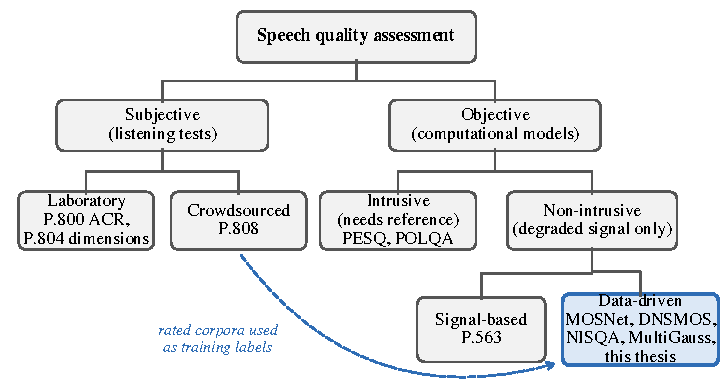
\includegraphics[width=\textwidth]{figures/thesis/sqa_taxonomy.pdf}
  \caption{Overview of speech quality assessment methods. Data-driven non-intrusive models, the kind studied in this thesis (highlighted), are trained on corpora rated in subjective tests.}
  \label{fig:sqaTaxonomy}
\end{figure}

The two families depend on each other. An objective model is trained and validated on subjective ratings, so it can be no better than the ratings it learns from, and its usefulness is limited by how much rated data exists. This thesis is about data-driven non-intrusive SQA, and about how the subjective data available for training such models can be used more fully.

\subsection{Challenges of data-driven assessment}
\label{sec:sqaChallenges}

Data-driven SQA models face four challenges that are relevant to this thesis:
\begin{description}
\item[Scarce labels.] Every label requires several listeners to rate a clip, so rated corpora are expensive to build. Corpora with ratings of the quality dimensions are especially rare, because each clip has to be rated on five scales instead of one (Section~\ref{sec:qualityDimensions}).
\item[Different scales.] Corpora rated in separate listening tests do not use the rating scale in exactly the same way, which makes it difficult to train one model on several corpora (Section~\ref{sec:corpusEffects}).
\item[Generalisation.] A model trained on one corpus often performs worse on speech from other systems, languages or listening tests. It is therefore important to evaluate on corpora that were not used for training.
\item[Uncertainty.] Listeners disagree, and some clips are rated far more consistently than others. A single predicted score hides this, which motivates probabilistic models that also predict their uncertainty (Section~\ref{sec:probabilistic}).
\end{description}
This thesis addresses mainly the first challenge, by combining multidimensional data with MOS-only data. Because the combined corpora were rated in separate tests, the second challenge comes with it. The third is addressed by evaluating on unseen corpora, and the fourth by building on a probabilistic model.

\section{Subjective speech quality}
\label{sec:subjectiveQuality}

\subsection{Mean opinion score}

As Section~\ref{sec:whatIsQuality} explained, the reference method for measuring speech quality is a listening test. ITU-T Recommendation P.800~\cite{itu_p800} describes the most common procedure, the \gls{ACR} test. Listeners hear one speech clip at a time and rate its quality on a five-point scale: 5 (excellent), 4 (good), 3 (fair), 2 (poor) and 1 (bad). The \gls{MOS} of a clip is the average of the ratings it receives. 

Laboratory listening tests are slow and expensive, because they require a controlled environment and a panel of listeners. ITU-T P.808~\cite{itu_p808} therefore specifies how to run ACR tests through crowdsourcing, where many listeners rate clips over the internet with their own equipment. Crowdsourcing makes large rated corpora possible, and the corpora used in this thesis were rated in this way~\cite{mittag_nisqa_2021,mittag_pstn_2020}.

\subsection{Quality dimensions}
\label{sec:qualityDimensions}

MOS states how good a clip sounds, but not why. ITU-T P.804~\cite{itu_p804} defines a diagnostic test in which listeners also rate four perceptual \emph{quality dimensions}, each on a five-point scale where a higher value means better quality:
\begin{description}
\item[Noisiness (NOI)] how much the speech is disturbed by background noise, circuit noise or coding noise.
\item[Coloration (COL)] how much the timbre of the voice is altered, for example by bandwidth limitation or a poor frequency response.
\item[Discontinuity (DIS)] how much the speech is interrupted or distorted in time, for example by packet loss or clipping.
\item[Loudness (LOUD)] how far the level of the speech is from a comfortable listening level, whether too quiet or too loud.
\end{description}
These dimensions follow earlier research on the perceptual space of transmitted speech, which found that its quality can be described largely by a small number of underlying dimensions~\cite{waltermann_2010}. Rating all four dimensions in addition to the overall quality makes each rating task longer and requires listeners to understand the difference between the dimensions. This is one reason why multidimensional data is much scarcer than MOS-only data.

\subsection{Differences between corpora}
\label{sec:corpusEffects}

A MOS value is not an absolute quantity. The same clip can receive a different score in two tests, because listeners judge each clip partly in relation to the other clips they hear in the same test. If a test contains mostly poor-quality clips, a medium-quality clip tends to be rated higher than it would be in a test with mostly good clips. The listener panel, the instructions, the listening equipment and the language also influence the ratings, so a MOS holds only for the listeners and the test design with which it was obtained~\cite{itu_p1401,mittag_biasaware_2021}. As a result, two corpora rated in different tests may use the MOS scale differently, even if both follow the ACR procedure. A model trained on several corpora must therefore learn from labels whose scales do not fully agree. This matters for the two-stage model, which is trained on NISQA and PSTN, two corpora rated in separate tests with different sets of conditions.

\section{The relation between MOS and the quality dimensions}
\label{sec:mosAndDimensions}

The two-stage model rests on the assumption that MOS depends on the four quality dimensions (Section~\ref{sec:researchQuestion}). The P.804 dimensions were designed to describe the ways in which a speech signal can be degraded, so the overall quality can be expected to reflect their combined effect. The NISQA training labels support this assumption. Table~\ref{tab:mosDimCorrelation} shows the Pearson correlation between MOS and each dimension in the two NISQA training sets, together with the share of the MOS variance that a linear combination of the four dimensions explains ($R^2$).

\begin{table}[!ht]
  \centering
  \caption{Relation between MOS and the four quality dimensions in the NISQA training labels: Pearson correlation between MOS and each dimension, and the coefficient of determination $R^2$ of a linear regression of MOS on all four dimensions.}
  \label{tab:mosDimCorrelation}
  \setlength{\tabcolsep}{4pt}
  \begin{adjustbox}{max width=\textwidth}
  \begin{tabular}{lrrrrrr}
    \toprule
    Training set & Clips & NOI & COL & DIS & LOUD & $R^2$ \\
    \midrule
    NISQA\_TRAIN\_SIM  & 10\,000 & 0.67 & 0.81 & 0.73 & 0.81 & 0.87 \\
    NISQA\_TRAIN\_LIVE & 1\,020  & 0.50 & 0.60 & 0.58 & 0.76 & 0.76 \\
    \bottomrule
  \end{tabular}
  \end{adjustbox}
\end{table}

Each dimension correlates positively with MOS, so when the rating of a dimension goes up or down, MOS tends to follow. Together, the four dimensions explain 87\,\% of the MOS variance in the simulated training set and 76\,\% in the live set, using only a linear combination. The relation is weaker for the live calls, where degradations are more varied and the labels are noisier. The part of MOS that the four dimensions do not explain is one reason why the MOS stage of the two-stage model also receives the speech features (Chapter~\ref{ch:whatYouDid}).

Table~\ref{tab:mosDimCorrelation} and Figure~\ref{fig:mosDimCorrelation} also show that the dimensions are related to MOS, but not interchangeable with it. The dimensions correlate less with each other than with MOS (for example, 0.39 between NOI and DIS in the simulated set), which confirms that they capture different types of degradation.

\begin{figure}[!ht]
  \centering
  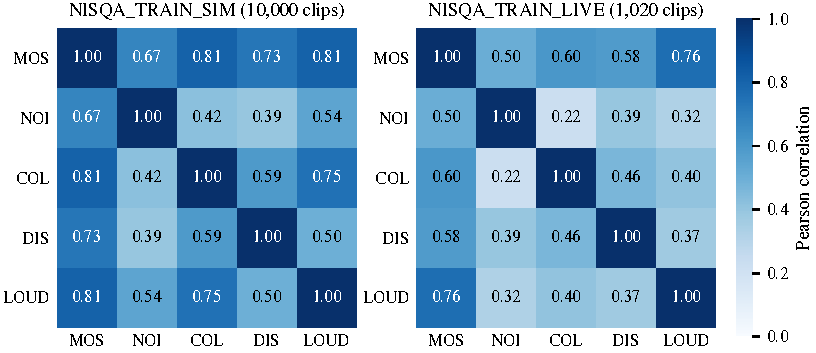
\includegraphics[width=\textwidth]{figures/thesis/mos_dim_correlation.pdf}
  \caption{Pearson correlation between MOS and the four quality dimensions, and between the dimensions themselves, in the two NISQA training sets.}
  \label{fig:mosDimCorrelation}
\end{figure}


\section{Objective speech quality models}
\label{sec:objectiveModels}

Objective speech quality models predict the result of a listening test from the speech signal. As shown in Figure~\ref{fig:sqaTaxonomy}, they are divided into \emph{intrusive} and \emph{non-intrusive} models.

\subsection{Intrusive models}

Intrusive models compare the degraded signal with the clean reference signal it was derived from. The best known are \gls{PESQ}, ITU-T P.862~\cite{itu_p862}, and its successor \gls{POLQA}, ITU-T P.863~\cite{itu_p863}. Both align the two signals in time, transform them into a perceptual representation, and map the difference between them to a MOS estimate. Intrusive models are accurate when a reference is available, but in a live call or a recording made in the field, the clean reference does not exist.

\subsection{Non-intrusive models}

Non-intrusive models predict quality from the degraded signal alone. Early examples, such as ITU-T P.563~\cite{itu_p563}, combined hand-crafted signal features with rules. Most current non-intrusive models are deep neural networks trained on rated corpora. MOSNet~\cite{lo_mosnet_2019} used a convolutional and recurrent network on spectrograms to predict the quality of converted speech. DNSMOS~\cite{reddy_dnsmos_2021} predicts the quality of noise-suppressed speech with a convolutional network trained on a large crowdsourced corpus. NISQA~\cite{mittag_nisqa_2021} combines a convolutional network with self-attention, and was the first widely used model to predict the four P.804 dimensions together with MOS. It was trained on the NISQA corpus, which was released with it and is also the multidimensional corpus used in this thesis.

\section{Self-supervised speech representations}
\label{sec:ssl}

Training a deep network from raw audio needs a lot of labelled data, and rated speech quality data is limited. Self-supervised learning reduces this need. A model is first pre-trained on large amounts of unlabelled speech with a task that needs no human labels, and the representations it learns are then reused for other tasks.

wav2vec~2.0~\cite{baevski_wav2vec2_2020} is a widely used self-supervised model. A convolutional encoder turns the waveform into a sequence of latent frames, about one every 20\,ms, and a transformer network processes the sequence. During pre-training, part of the latent sequence is masked, and the model learns to identify the correct latent frame at each masked position among a set of distractors. XLS-R~\cite{babu_xlsr_2022} scales this approach to 436\,000 hours of speech in 128 languages, with models of up to two billion parameters.

The output of each transformer layer of such a model can be used as a sequence of feature vectors. Different layers capture different information: lower layers are closer to the acoustic signal, and higher layers are closer to phonetic and linguistic content. Features from self-supervised models have been shown to improve MOS prediction considerably, especially for data that differs from the training data~\cite{cooper_bvcc_2022}. MultiGauss~\cite{cumlin_multigauss_2025} uses the output of one intermediate layer of the two-billion-parameter XLS-R model, without fine-tuning, and this thesis uses the same features.

\section{Probabilistic regression}
\label{sec:probabilistic}

A standard regression model predicts a single value for each input and is trained to minimise, for example, the squared error. A \emph{probabilistic} regression model instead predicts a probability distribution over the target. This gives an estimate of how uncertain the prediction is, which is useful for speech quality, where the listeners themselves disagree and some clips are harder to judge than others.

\subsection{Gaussian negative log-likelihood}

The simplest choice is a Gaussian distribution. For an input $\vect{x}$, the model predicts a mean $\mu(\vect{x})$ and a variance $\sigma^2(\vect{x})$, and is trained to minimise the \gls{GNLL} of the target $y$~\cite{nix_weigend_1994}:
\begin{equation}
  \mathcal{L}_{\text{GNLL}} = \frac{1}{2}\log \sigma^2(\vect{x}) + \frac{\big(y - \mu(\vect{x})\big)^2}{2\,\sigma^2(\vect{x})} + \text{const.}
  \label{eq:gnll}
\end{equation}
The second term is a squared error scaled by the predicted variance, so the model can lower the penalty on a hard example by predicting a larger variance. The first term penalises large variances, so the model cannot do this everywhere. The predicted variance therefore captures the uncertainty that remains in the data, known as \emph{aleatoric} uncertainty~\cite{kendall_gal_2017}.

\subsection{Multivariate Gaussian}

When several quantities are predicted together, such as MOS and the four dimensions, the model can predict a multivariate Gaussian with mean vector $\vect{\mu}(\vect{x}) \in \mathbb{R}^d$ and covariance matrix $\vect{\Sigma}(\vect{x}) \in \mathbb{R}^{d \times d}$. The covariance describes the uncertainty of each quantity and also how the errors of different quantities are related. The loss is the multivariate GNLL:
\begin{equation}
  \mathcal{L} = \frac{1}{2}\log \det \vect{\Sigma}(\vect{x}) + \frac{1}{2}\big(\vect{y} - \vect{\mu}(\vect{x})\big)^{\top} \vect{\Sigma}(\vect{x})^{-1} \big(\vect{y} - \vect{\mu}(\vect{x})\big) + \text{const.}
  \label{eq:mvgnll}
\end{equation}
A covariance matrix must be symmetric and positive definite, which an unconstrained network output does not guarantee. A common solution is to predict a lower-triangular matrix $\vect{L}$ with positive diagonal elements and form $\vect{\Sigma} = \vect{L}\vect{L}^{\top}$, the \emph{Cholesky} parameterisation. For $d$ quantities, the network outputs $d$ means and $d(d+1)/2$ elements of $\vect{L}$.

\subsection{MultiGauss}
\label{sec:multigaussBackground}

MultiGauss~\cite{cumlin_multigauss_2025} applies this approach to speech quality. It takes XLS-R features of a clip, passes them through two convolutional layers and three fully connected layers, and outputs a five-dimensional Gaussian over MOS, NOI, COL, DIS and LOUD: five means and 15 Cholesky elements. It is trained with the loss in Equation~\eqref{eq:mvgnll} on the NISQA corpus. Because the loss involves all five quantities, every training clip must have all five labels. MultiGauss is the baseline in this thesis, and its architecture is described in more detail in Chapter~\ref{ch:methods}.

\section{Learning from partially labelled data}
\label{sec:partialLabels}

When some training examples lack some labels, there are two common ways to still use them.

\subsection{Masking missing labels}

The simplest way is to keep a single model that predicts all outputs and to leave the missing labels out of the loss. Each missing label is marked, for example as \gls{NaN}, and a mask removes the corresponding terms from the loss, so only the available labels produce gradients. Wang et~al.~\cite{wang_urgentmos_2026} use such a masked loss to train a speech quality model on corpora with different sets of labels, normalising each metric's loss by the number of valid labels. For a Gaussian model, the equivalent is to evaluate the likelihood of the \emph{marginal} distribution of the observed labels, which for a multivariate Gaussian is obtained by keeping only the corresponding entries of $\vect{\mu}$ and $\vect{\Sigma}$. This approach is the baseline for RQ3.

\subsection{Multi-task and cascaded models}

The second way is to structure the model so that different parts are trained by different labels. In \emph{multi-task learning}, several tasks share part of a network, typically the feature encoder, and each task has its own output head~\cite{caruana_multitask_1997}. Each training example then updates the shared part and the heads for which it has labels. Learning related tasks together can improve each of them, because the shared representation must be useful for all of them.

A \emph{cascaded} model goes one step further, by feeding the output of one head into another. The two-stage model in this thesis is of this kind: the first stage predicts the four dimensions, and the second stage uses them to predict MOS. Training a cascade raises a well-known question about what the second stage should receive. During training, it can receive the true values of the first-stage outputs, called \emph{teacher forcing}~\cite{williams_zipser_1989}, which gives clean inputs and fast learning. At test time, however, only the first stage's predictions are available, and they contain errors the second stage never saw during training. \emph{Scheduled sampling}~\cite{bengio_scheduled_2015} addresses this mismatch by gradually replacing the true values with predictions during training. Both options are examined for the two-stage model in Chapter~\ref{ch:resultsAndAnalysis}.

\section{Related work}
\label{sec:relatedWork}

Several earlier works use more than one corpus to train a MOS model. Mittag et~al.~\cite{mittag_biasaware_2021} train on several corpora together and handle their different MOS scales with a \emph{bias-aware} loss, which learns a mapping between the model's prediction and each corpus's scale. Other models include the listener or the corpus as an extra input, so that the model can learn their individual biases. MBNet~\cite{leng_mbnet_2021} and LDNet~\cite{huang_ldnet_2022} do this for individual listeners. These methods aim to correct for differences between corpora, which is outside the scope of this thesis (Section~\ref{sec:researchQuestion}). This thesis instead studies how much combined training helps without such corrections.

Multidimensional models are fewer. NISQA~\cite{mittag_nisqa_2021} predicts the five quantities with separate output heads on a shared network, and MultiGauss~\cite{cumlin_multigauss_2025} predicts them jointly as a single distribution. Both are trained on fully labelled data only. Wang et~al.~\cite{wang_urgentmos_2026} show that a masked loss lets a single model learn from corpora with different label sets, but to the author's knowledge, no earlier work has examined whether adding MOS-only data also improves the prediction of the P.804 dimensions, which is the focus of RQ2.

\section{Summary}
\label{sec:backgroundSummary}

Speech quality is a listener's judgement, so SQA rests on listening tests, and objective models learn to predict their results. Data-driven models are limited above all by how much rated data exists. Speech quality is measured in listening tests as a MOS, and P.804 adds four quality dimensions that explain the overall quality. In the NISQA labels, a linear combination of the four dimensions explains most of the MOS variance, which supports the assumption behind the two-stage model. MOS values from different corpora are not on exactly the same scale, which is a challenge for any model trained on combined data. Modern non-intrusive models use features from large self-supervised speech models, and MultiGauss predicts all five quantities as one multivariate Gaussian. Since a joint model needs all five labels, MOS-only data can be used either by masking missing labels or by a multi-task or cascaded design. The two-stage model uses a cascaded design.

\cleardoublepage
\chapter{Method}
\label{ch:methods}

This chapter describes how the research questions were investigated. Section~\ref{sec:researchProcess} gives an overview of the research process. Section~\ref{sec:datasets} presents the datasets and Section~\ref{sec:features} the input features. Section~\ref{sec:baselines} describes the baseline models, Section~\ref{sec:experimentalDesign} the experiments, and Section~\ref{sec:evaluation} how the models were evaluated. Section~\ref{sec:reliabilityValidity} discusses the reliability and validity of the method. The proposed two-stage model itself is described in Chapter~\ref{ch:whatYouDid}.

\section{Research process}
\label{sec:researchProcess}

The work followed the five steps shown in Figure~\ref{fig:researchProcess}:
\begin{enumerate}
\item \textbf{Reproduce the baseline.} The published MultiGauss model was evaluated with the same features and evaluation code as all later models, to confirm that the pipeline reproduces the published results.
\item \textbf{Build the two-stage model.} The model was designed so that MOS-only clips can train it together with fully labelled clips (Chapter~\ref{ch:whatYouDid}).
\item \textbf{Design studies.} The main design choices, such as the structure of the MOS stage and the mix of corpora in a training batch, were varied one at a time to decide the final configuration.
\item \textbf{Main experiments.} The final two-stage model was compared with the baselines in two experiments, one with a separate MOS-only corpus and one with a MOS-only subset of the same corpus.
\item \textbf{Statistical evaluation.} The differences between models were tested for significance, to separate real effects from training randomness.
\end{enumerate}

\begin{figure}[!ht]
  \centering
  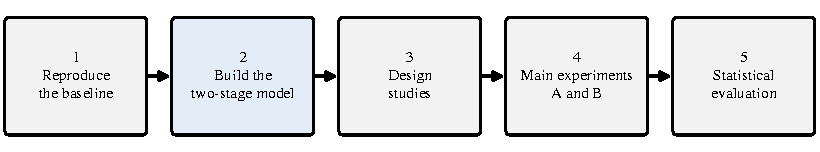
\includegraphics[width=\textwidth]{figures/thesis/research_process.pdf}
  \caption{The research process followed in this thesis.}
  \label{fig:researchProcess}
\end{figure}

\section{Datasets}
\label{sec:datasets}

\subsection{NISQA corpus}

The NISQA corpus~\cite{mittag_nisqa_2021} is the source of all multidimensional labels in this thesis. Each clip has crowdsourced ratings for MOS and for the four P.804 dimensions, collected with on average about five ratings per clip and averaged into one score per quantity. The clips are English speech, about 6--12 seconds long. Table~\ref{tab:nisqaSplits} lists the parts used.

\begin{table}[!ht]
  \centering
  \caption{Parts of the NISQA corpus used in this thesis. All parts have labels for MOS and the four quality dimensions.}
  \label{tab:nisqaSplits}
  \begin{adjustbox}{max width=\textwidth}
  \begin{tabular}{llrl}
    \toprule
    Part & Distortions & Clips & Use \\
    \midrule
    NISQA\_TRAIN\_SIM   & simulated & 10\,000 & training \\
    NISQA\_TRAIN\_LIVE  & live calls & 1\,020 & training \\
    NISQA\_VAL\_SIM     & simulated & 2\,500 & checkpoint selection, evaluation \\
    NISQA\_VAL\_LIVE    & live calls & 200 & checkpoint selection, evaluation \\
    NISQA\_TEST\_FOR      & simulated and live & 240 & evaluation only \\
    NISQA\_TEST\_P501     & simulated and live & 240 & evaluation only \\
    NISQA\_TEST\_LIVETALK & live recordings & 232 & evaluation only \\
    \bottomrule
  \end{tabular}
  \end{adjustbox}
\end{table}

The \emph{simulated} parts (SIM) were created by passing clean speech through simulated transmission and processing, such as codecs, packet loss, noise, filtering and level changes, so they cover a wide range of quality. The \emph{live} parts (LIVE) are real calls made over Skype and from landlines to mobile phones. The 1\,020 LIVE training clips come from 495 different source recordings.

The SIM and LIVE parts have quite different label distributions, which is important for Experiment~B (Section~\ref{sec:expB}). Table~\ref{tab:simLiveStats} and Figure~\ref{fig:simLiveDistributions} compare the two training sets. The LIVE clips are rated clearly lower than the SIM clips for MOS, coloration and loudness, and they span a narrower range of scores. Fewer than 1\,\% of the LIVE clips have a MOS of 4 or higher, compared with about 25\,\% of the SIM clips. Discontinuity is the only dimension with a similar distribution in both parts. A narrow range of true scores also makes correlation-based metrics lower, so scores on LIVE data are expected to be lower than on SIM data for every model.

\begin{figure}[!ht]
  \centering
  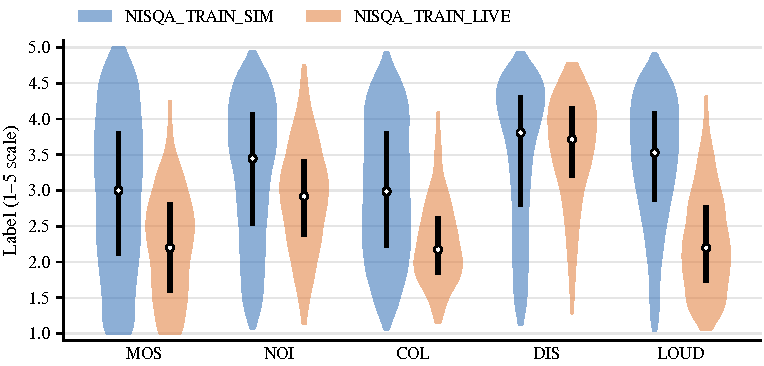
\includegraphics[width=\textwidth]{figures/thesis/sim_live_distributions.pdf}
  \caption{Distribution of the labels in the two NISQA training sets. The black bar spans the middle 50\,\% of the clips (interquartile range), and the white dot marks the median.}
  \label{fig:simLiveDistributions}
\end{figure}

\begin{table}[!ht]
  \centering
  \caption{Mean and standard deviation of the labels in the two NISQA training sets.}
  \label{tab:simLiveStats}
  \begin{adjustbox}{max width=\textwidth}
  \begin{tabular}{lcc}
    \toprule
    Quantity & NISQA\_TRAIN\_SIM & NISQA\_TRAIN\_LIVE \\
    \midrule
    MOS  & 2.98 (1.10) & 2.23 (0.70) \\
    NOI  & 3.27 (0.96) & 2.91 (0.71) \\
    COL  & 3.01 (0.93) & 2.25 (0.53) \\
    DIS  & 3.51 (0.97) & 3.61 (0.69) \\
    LOUD & 3.42 (0.84) & 2.26 (0.67) \\
    \bottomrule
  \end{tabular}
  \end{adjustbox}
\end{table}

\subsection{PSTN corpus}

The PSTN corpus~\cite{mittag_pstn_2020} contains real telephone calls made over the \gls{PSTN} and \gls{VoIP}, rated with crowdsourced ACR tests. It has MOS labels only, so it serves as the MOS-only corpus in Experiment~A. Because of storage limits, two subsets were drawn from it, each stratified by MOS so that the score distribution of the full set is preserved:
\begin{itemize}
\item \textbf{PSTN\_TRAIN12K}: 12\,000 clips from the PSTN training set, used for training (mean MOS 3.12, standard deviation 0.87).
\item \textbf{PSTN\_VAL2K}: 2\,000 clips from the PSTN validation set, used only for evaluation.
\end{itemize}

\subsection{BVCC}

BVCC~\cite{cooper_ssw_2021} contains synthetic speech from \gls{TTS} and voice conversion systems, rated for naturalness on a MOS scale. Its validation set of 387 clips is used only to evaluate how well the models generalise to a domain none of them was trained on.

\subsection{Overlap check}

Before evaluation, the data was checked for overlap between training and evaluation sets. The NISQA validation sets share no clips and no source recordings with the NISQA training sets, and PSTN\_VAL2K shares no clips with PSTN\_TRAIN12K.

\section{Feature extraction}
\label{sec:features}

All models use the same input features, taken from the two-billion-parameter XLS-R model~\cite{babu_xlsr_2022}, the same feature extractor as MultiGauss~\cite{cumlin_multigauss_2025}. Each clip is resampled to 16\,kHz and passed through XLS-R, and the output of the 12th transformer layer is kept: a sequence of 1\,920-dimensional vectors, one per 20\,ms. XLS-R is not fine-tuned, so the features were computed once for every clip and stored on disk, which makes training much faster and identical for all models.

Clips shorter than 10 seconds are repeated until they reach 10 seconds, and longer clips are cut, so every clip gives a feature sequence of the same length. The original MultiGauss work uses 8 seconds. The longer crop was kept for all models trained in this thesis, so the comparisons between them are not affected.

The choice of layer was examined in an early design study (Section~\ref{sec:designStudies}).

\section{Baseline models}
\label{sec:baselines}

\subsection{MultiGauss}

MultiGauss~\cite{cumlin_multigauss_2025} is the main baseline (Section~\ref{sec:multigaussBackground}). Its architecture is:
\begin{itemize}
\item two one-dimensional convolutional layers with 32 channels and kernel size 5, each followed by layer normalisation, a \gls{ReLU} activation, dropout of 0.3 and max pooling by a factor of 5;
\item three fully connected layers with 64, 32 and 20 outputs;
\item the 20 outputs give 5 means and the 15 elements of a lower-triangular Cholesky factor, which form a five-dimensional Gaussian over MOS, NOI, COL, DIS and LOUD.
\end{itemize}
It is trained with the multivariate Gaussian negative log-likelihood (Equation~\eqref{eq:mvgnll}) on clips that have all five labels.

The published MultiGauss checkpoint, trained on all NISQA training data, was evaluated with the pipeline of this thesis. Its average PCC over the five quantities on the three test sets was 0.838 (LIVETALK), 0.824 (FOR) and 0.855 (P501), against 0.834, 0.829 and 0.862 in the original paper. The pipeline therefore reproduces the published results to within about 0.007.

\subsection{MultiGauss trained on simulated data only}

For Experiment~B, MultiGauss was also trained from scratch on NISQA\_TRAIN\_SIM only, using its own training procedure: 64 clips per step, 350 steps per epoch, up to 30 epochs, and the Adam optimiser~\cite{kingma_adam_2015} with a learning rate of $10^{-4}$. This is the \emph{multidimensional data alone} baseline: it sees exactly the same fully labelled data as the two-stage model in that experiment, but none of the MOS-only data.

\subsection{MultiGauss with a masked loss}
\label{sec:nanBaseline}

The baseline for RQ3 is MultiGauss trained on fully labelled and MOS-only clips together, with the missing labels masked out (Section~\ref{sec:partialLabels}). Each batch holds 32 NISQA\_TRAIN\_SIM clips with all five labels and 32 NISQA\_TRAIN\_LIVE clips whose four dimension labels are set to NaN. For each clip, the loss is the negative log-likelihood of the \emph{marginal} Gaussian over the labels that are present. For a fully labelled clip this is the normal MultiGauss loss, and for a MOS-only clip it is the univariate Gaussian loss on MOS:
\begin{equation}
  \mathcal{L}_{\text{MOS-only}} = \frac{1}{2}\log \Sigma_{\text{MOS,MOS}} + \frac{\big(y_{\text{MOS}} - \mu_{\text{MOS}}\big)^2}{2\,\Sigma_{\text{MOS,MOS}}} + \text{const.}
  \label{eq:marginalLoss}
\end{equation}
Everything else is the same as for MultiGauss trained on SIM only. This baseline follows the masked loss proposed in URGENT-MOS~\cite{wang_urgentmos_2026}, adapted to a Gaussian model. It uses the same data as the two-stage model but no special architecture, so it shows how much of any gain comes from the data itself.

\section{Experimental design}
\label{sec:experimentalDesign}

\subsection{Training settings}

Unless stated otherwise, all models in this thesis share the following settings. Each training step uses a batch of 64 clips, made up of 32 fully labelled clips and 32 MOS-only clips for the two-stage model. An epoch has 350 steps, and training runs for at most 30 epochs with the Adam optimiser and a learning rate of $10^{-4}$. Training stops early if the validation result has not improved for 15 epochs. After each epoch, the model is evaluated on the NISQA validation sets, and the weights from the epoch with the highest MOS PCC are kept.

\subsection{Experiment A: adding a separate MOS-only corpus}
\label{sec:expA}

Figure~\ref{fig:experimentsAB} gives an overview of the training and evaluation data in the two main experiments.

\begin{figure}[!ht]
  \centering
  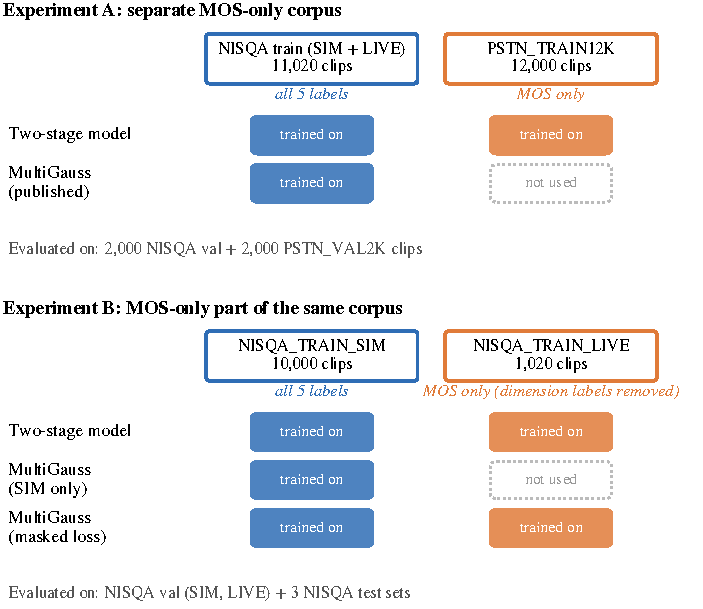
\includegraphics[width=\textwidth]{figures/thesis/experiments_ab.pdf}
  \caption{The training data of each model in Experiments A and B, and the data they are evaluated on.}
  \label{fig:experimentsAB}
\end{figure}


Experiment~A tests whether a MOS-only corpus recorded and rated separately from the multidimensional corpus helps the model. This is the realistic case: in practice, extra MOS-only data will come from a different test, with different listeners and conditions.
\begin{itemize}
\item \textbf{Two-stage model:} trained on all NISQA training data (SIM and LIVE, with all five labels) together with PSTN\_TRAIN12K (MOS only).
\item \textbf{Baseline:} the published MultiGauss checkpoint, trained on all NISQA training data.
\item \textbf{Evaluation:} a combined set of 2\,000 NISQA validation clips and all 2\,000 PSTN\_VAL2K clips. The NISQA clips are a fixed random draw from NISQA\_VAL\_SIM and NISQA\_VAL\_LIVE in their natural proportions (1\,852 and 148 clips). MOS is evaluated on the whole set and on each half; the four dimensions are evaluated on the NISQA validation sets.
\end{itemize}
The combined set measures whether a model places clips from both corpora on one consistent MOS scale, which per-corpus metrics cannot show. Experiment~A mainly answers RQ1.

\subsection{Experiment B: a MOS-only subset of the same corpus}
\label{sec:expB}

Experiment~B tests the same idea under controlled conditions, by turning part of NISQA into MOS-only data. The 1\,020 LIVE training clips are used with their MOS label only, and their dimension labels are discarded.
\begin{itemize}
\item \textbf{Two-stage model:} trained on NISQA\_TRAIN\_SIM (all five labels) together with NISQA\_TRAIN\_LIVE (MOS only), 32 clips of each per batch.
\item \textbf{Baselines:} MultiGauss trained on NISQA\_TRAIN\_SIM only, and MultiGauss with the masked loss on the same data as the two-stage model (Section~\ref{sec:baselines}).
\item \textbf{Evaluation:} all five quantities on NISQA\_VAL\_SIM, NISQA\_VAL\_LIVE and the three NISQA test sets.
\end{itemize}
Since all the data comes from one corpus with one rating procedure, differences in MOS scale between corpora play no role. All models see exactly the same fully labelled data, so any difference in the dimension scores must come from the MOS-only data or from the way the model uses it. Experiment~B answers RQ2 and RQ3, and also gives a second answer to RQ1.

\subsection{Design studies}
\label{sec:designStudies}

The following studies were used to decide the configuration of the two-stage model. Each varies one factor and keeps the rest fixed. Their results are reported in Section~\ref{sec:designStudyResults}.
\begin{description}
\item[Structure of the MOS stage.] A MOS stage that receives only the four predicted dimensions is compared with one that also receives the encoded speech features.
\item[Teacher forcing or scheduled sampling.] During training, the MOS stage receives the true dimension values of the fully labelled clips (teacher forcing). This is compared with scheduled sampling~\cite{bengio_scheduled_2015}, where the true values are gradually replaced by the first stage's predictions, linearly over the first 20 of 30 epochs.
\item[Batch ratio, Experiment~A setting.] With the batch size fixed at 64, the number of PSTN clips per batch is varied from 11 to 43 (20\,\% to 200\,\% of the NISQA clips).
\item[Batch ratio, Experiment~B setting.] The SIM:LIVE split of a 64-clip batch is varied: 56:8, 48:16, 32:32, 16:48 and 63:1.
\item[Equal amounts of data.] Two checks of the Experiment~B result: a batch of 64 SIM plus 64 LIVE clips, so that the first stage sees as many fully labelled clips per step as MultiGauss does; and equal pools of 1\,020 SIM and 1\,020 LIVE clips, so that the LIVE clips are not repeated more often than the SIM clips.
\item[Amount of multidimensional data.] The two-stage model is trained on only 500 NISQA clips, first with different shares of PSTN clips in a fixed total of 500, and then with 200 to 1\,000 PSTN clips added. MultiGauss is trained on the same 500 NISQA clips for comparison.
\item[XLS-R layer.] Features from layers 12, 22 and 32 of XLS-R are compared.
\item[Hyperparameters.] The learning rate ($3\times10^{-5}$ to $10^{-3}$, constant or cosine schedule), weight decay, dropout, and the weight of the dimension loss relative to the MOS loss are varied. Each setting is chosen on the validation sets and reported on the test sets.
\end{description}
The XLS-R layer study and the first batch ratio study were single training runs, carried out early in the project. Their results are therefore indicative only. All other studies used three runs per configuration.

\section{Evaluation}
\label{sec:evaluation}

\subsection{Metrics}

Each model is evaluated separately for MOS and each of the four dimensions, using the per-clip predicted means. Let $y_n$ and $\hat{y}_n$ denote the true and the predicted score of clip $n$ in a set of $N$ clips, with means $\bar{y}$ and $\bar{\hat{y}}$. The main metric is the \gls{PCC},
\begin{equation}
  \rho = \frac{\sum_{n}\big(y_n - \bar{y}\big)\big(\hat{y}_n - \bar{\hat{y}}\big)}{\sqrt{\sum_{n}\big(y_n - \bar{y}\big)^2 \, \sum_{n}\big(\hat{y}_n - \bar{\hat{y}}\big)^2}},
  \label{eq:pcc}
\end{equation}
which measures how well the predictions follow the true scores. It does not change when the predictions are shifted or scaled by a positive factor, so it shows whether the model ranks the clips correctly, but not whether its values are correct. The \gls{RMSE},
\begin{equation}
  \mathrm{RMSE} = \sqrt{\frac{1}{N}\sum_{n}\big(\hat{y}_n - y_n\big)^2},
  \label{eq:rmse}
\end{equation}
is also reported, as it measures the error on the original rating scale and therefore captures the offsets and scaling that the \gls{PCC} ignores. As a single summary of the multidimensional performance, the average of the five PCCs is used, as in the MultiGauss paper~\cite{cumlin_multigauss_2025}.

\subsection{Evaluation sets}

Results are reported for each evaluation set on its own, and for sets combined (\emph{pooled}) into one. Pooling several sets tests whether the model's scores are consistent across them, because a clip from one set is ranked against clips from the others. Pooling is used for the three NISQA test sets, the two NISQA validation sets, and the NISQA and PSTN mix of Experiment~A.

\subsection{Repeated runs and significance}

Training a neural network involves randomness, from the initial weights, the order of the batches and dropout. Each configuration was therefore trained three times, with no fixed random seed, and results are given as the mean over the three runs.

Whether a difference between two models is real is tested with a \emph{hierarchical bootstrap}, which accounts for both sources of variation: the training runs and the evaluation clips. In each of 10\,000 bootstrap rounds, the training runs of each model are resampled with replacement, then the evaluation clips are resampled with replacement, and the metric difference is recomputed. Both models use the same resampled clips, and for pooled sets the clips are resampled within each set, so that its composition stays the same. The \emph{p}-value is the share of rounds in which the difference has the opposite sign to the observed one, doubled for a two-sided test. Because many comparisons are made, the \emph{p}-values in each table are adjusted with the Holm method~\cite{holm_1979}, and a difference is called significant if its adjusted \emph{p}-value is below 0.05.

\section{Reliability and validity}
\label{sec:reliabilityValidity}

Several measures were taken to make the results reliable and the comparisons fair:
\begin{itemize}
\item All models use the same features, the same evaluation code and, where they are trained in this thesis, the same training schedule.
\item The evaluation pipeline was checked against the published MultiGauss results.
\item Every configuration was trained three times, and differences were tested for significance rather than judged from the means.
\item The test sets were never used for selecting checkpoints or for choosing hyperparameters in the tuning. The early design studies report test-set results, but none of them changed the default configuration (Section~\ref{sec:designStudyResults}).
\end{itemize}

The method also has limitations. The checkpoint of every model is selected on NISQA validation MOS, so results on the validation sets are slightly optimistic, for the baselines and the two-stage model alike. The test sets are not affected, so the main conclusions are drawn from them where possible. Three runs per configuration give a rough estimate of the training variation, and small differences may go undetected. Finally, NISQA and PSTN are the only multidimensional and MOS-only training corpora used, so the conclusions may not carry over unchanged to other corpora.

\cleardoublepage
\chapter{The Two-Stage Model}
\label{ch:whatYouDid}

This chapter describes the model proposed in this thesis. Section~\ref{sec:modelOverview} explains the idea behind it, Sections~\ref{sec:sharedEncoder} to~\ref{sec:mosStage} describe its parts, and Section~\ref{sec:training} explains how it is trained on fully labelled and MOS-only clips together. Section~\ref{sec:inference} describes how it is used at test time, Section~\ref{sec:comparisonMultiGauss} compares it with MultiGauss, and Section~\ref{sec:implementation} gives implementation details.

\section{Overview and motivation}
\label{sec:modelOverview}

The model is built on the assumption stated in Section~\ref{sec:researchQuestion}: that MOS depends on the four quality dimensions. The NISQA labels support this, since a linear combination of the four dimensions explains 87\,\% of the MOS variance in the simulated training data and 76\,\% in the live data (Section~\ref{sec:mosAndDimensions}). The model therefore predicts quality in two stages, as shown in Figure~\ref{fig:twoStageModel}. The first stage predicts the four dimensions from the speech features. The second stage predicts MOS from those four dimensions together with the speech features.

This structure has a practical consequence, which is the main reason for the design. A model that predicts all five quantities jointly needs all five labels for every training clip. In the two-stage model, the MOS stage produces its own output and has its own loss, so a clip with only a MOS label can still be used to train it. Fully labelled clips and MOS-only clips can therefore be mixed in the same training batch.

The structure also makes it possible to test the second hypothesis of this thesis: that if MOS depends on the dimensions, learning to predict MOS better should also improve the dimension predictions. As Section~\ref{sec:training} explains, the error on a MOS-only clip flows back through the predicted dimensions into the first stage, so the MOS-only data can in principle influence the dimension predictions.

\begin{figure}[!ht]
  \centering
  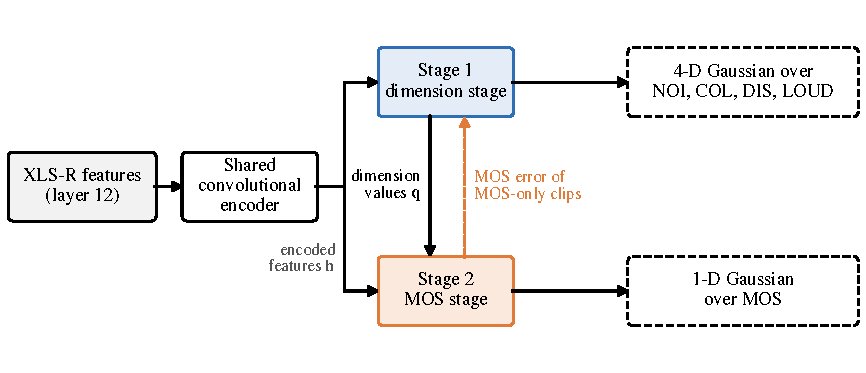
\includegraphics[width=\textwidth]{figures/thesis/two_stage_model.pdf}
  \caption{The two-stage model. The shared encoder processes the XLS-R features once. Stage~1 predicts a Gaussian over the four quality dimensions, and Stage~2 predicts MOS from the encoded features $\vect{h}$ and the four dimension values $\vect{q}$. During training, Stage~2 receives the true dimension values for fully labelled clips and Stage~1's predictions for MOS-only clips; for the MOS-only clips, the MOS error also flows back into Stage~1 (dashed arrow). At test time, Stage~2 always receives Stage~1's predictions.}
  \label{fig:twoStageModel}
\end{figure}

\section{Shared encoder}
\label{sec:sharedEncoder}

The input to the model is the sequence of XLS-R feature vectors described in Section~\ref{sec:features}. A shared encoder turns this sequence into a shorter, more compact representation. It consists of two one-dimensional convolutional layers with 32 channels and kernel size 5. Each is followed by layer normalisation, a ReLU activation, dropout with probability 0.3, and max pooling by a factor of 5. The encoder is the same as the convolutional part of MultiGauss~\cite{cumlin_multigauss_2025}, so the two models differ only in how the encoded representation is turned into quality predictions.

The encoder runs once for each clip, and its output $\vect{h}$ is used by both stages. Both stages therefore send their training signal back into the same encoder.

\section{Stage 1: the dimension stage}
\label{sec:dimensionStage}

The first stage predicts the four quality dimensions. It flattens the encoder output and passes it through three fully connected layers with 64, 32 and 14 outputs, with ReLU activations between them. The 14 outputs define a four-dimensional Gaussian: 4 values for the mean vector $\vect{\mu}_d$, and 10 values for a lower-triangular Cholesky factor $\vect{L}_d$ (4 diagonal and 6 off-diagonal elements). A softplus function keeps the diagonal elements positive, so that $\vect{\Sigma}_d = \vect{L}_d\vect{L}_d^{\top}$ is a valid covariance matrix (Section~\ref{sec:probabilistic}).

As in MultiGauss, the network output is mapped onto the rating scale by an affine transformation. The mean becomes $2\vect{\mu}_d + 3$, so that an output of 0 corresponds to the middle of the 1--5 scale, and the covariance is scaled by 4 to match. In the rest of this chapter, $\vect{\mu}_d$ and $\vect{\Sigma}_d$ denote the values after this mapping.

\section{Stage 2: the MOS stage}
\label{sec:mosStage}

The second stage predicts MOS from two inputs:
\begin{enumerate}
\item \textbf{Four dimension values} $\vect{q} \in \mathbb{R}^4$, passed through two fully connected layers with 32 and 16 outputs and ReLU activations.
\item \textbf{The encoded speech features} $\vect{h}$, flattened into one vector.
\end{enumerate}
The two resulting vectors are concatenated and passed through fully connected layers with 64, 32 and 2 outputs. The two outputs give the MOS mean $\mu_m$ and, after a softplus function, its variance $\sigma_m^2$. The same affine mapping as in Stage~1 is applied: the mean becomes $2\mu_m + 3$, and the variance is scaled by 4. In short, Stage~2 computes
\begin{equation}
  \big(\mu_m, \sigma_m^2\big) = g\big(\vect{h}, \vect{q}\big).
  \label{eq:mosStage}
\end{equation}

The dimension values $\vect{q}$ are the main input, in line with the assumption that MOS depends on the dimensions. The encoded features are added because the four dimensions do not explain all of MOS: about 13\,\% of the MOS variance in the simulated training data, and 24\,\% in the live data, is not explained by a linear combination of them (Table~\ref{tab:mosDimCorrelation}). The features give Stage~2 access to the rest of the information in the signal. Section~\ref{sec:designStudyResults} compares this design with a MOS stage that receives only the four dimension values.

Figure~\ref{fig:architecture} shows the complete architecture layer by layer, with the size of each intermediate representation for a 10-second clip. The XLS-R features of a clip form a sequence of 500 vectors of 1\,920 values. Each convolutional layer without padding shortens the sequence by four frames and the pooling divides its length by five, so the encoder output has 32 channels and 19 time steps, which gives a flattened vector $\vect{h}$ of 608 values. In total, the model has about 0.43 million trainable parameters, most of them in the first convolutional layer.

\begin{figure}[!ht]
  \centering
  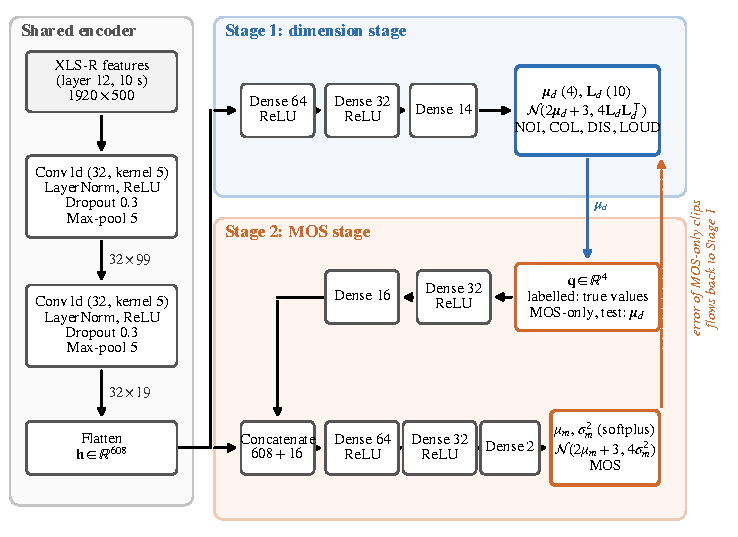
\includegraphics[width=\textwidth]{figures/thesis/architecture.pdf}
  \caption{Architecture of the two-stage model, layer by layer, with the size of each intermediate representation for a 10-second clip. All dense layers except the last one of each stage are followed by a ReLU activation. The input $\vect{q}$ of Stage~2 is the true dimension values for fully labelled clips during training and Stage~1's predicted means $\vect{\mu}_d$ otherwise. The dashed arrow shows the path along which the MOS error of MOS-only clips trains Stage~1.}
  \label{fig:architecture}
\end{figure}

\section{Training}
\label{sec:training}

\subsection{Two kinds of training clips}

Each training step uses a batch of $B_\ell = 32$ fully labelled clips and $B_m = 32$ MOS-only clips. The two kinds of clips are passed through the model differently, as summarised in Table~\ref{tab:trainingPaths}.

\begin{table}[!ht]
  \centering
  \caption{How the two kinds of training clips are used.}
  \label{tab:trainingPaths}
  \setlength{\tabcolsep}{4pt}
  \begin{adjustbox}{max width=\textwidth}
  \begin{tabular}{p{3.2cm}p{4.6cm}p{4.6cm}}
    \toprule
     & Fully labelled clip & MOS-only clip \\
    \midrule
    Stage 1 loss & 4-D Gaussian NLL on the four dimension labels & none (no dimension labels) \\
    Input $\vect{q}$ to Stage 2 & true dimension values $\vect{y}_d$ & Stage~1's predictions $\vect{\mu}_d$ \\
    Stage 2 loss & Gaussian NLL on the MOS label & Gaussian NLL on the MOS label \\
    \bottomrule
  \end{tabular}
  \end{adjustbox}
\end{table}

\subsection{Loss function}

For a fully labelled clip with dimension labels $\vect{y}_d$ and MOS label $y_m$, Stage~1 is trained with the four-dimensional Gaussian negative log-likelihood (Equation~\eqref{eq:mvgnll}):
\begin{equation}
  \ell_{d} = \frac{1}{2}\log\det\vect{\Sigma}_d + \frac{1}{2}\big(\vect{y}_d - \vect{\mu}_d\big)^{\top}\vect{\Sigma}_d^{-1}\big(\vect{y}_d - \vect{\mu}_d\big),
  \label{eq:dimLoss}
\end{equation}
and Stage~2 with the univariate Gaussian negative log-likelihood (Equation~\eqref{eq:gnll}) of the MOS label:
\begin{equation}
  \ell_{m} = \frac{1}{2}\log\big(2\pi\sigma_m^2\big) + \frac{\big(y_m - \mu_m\big)^2}{2\,\sigma_m^2}.
  \label{eq:mosLoss}
\end{equation}
For a fully labelled clip, Stage~2 receives the true dimension values, $\vect{q} = \vect{y}_d$. For a MOS-only clip, only $\ell_m$ is computed, and Stage~2 receives the dimensions predicted by Stage~1, $\vect{q} = \vect{\mu}_d$. The loss for one training step is the sum of three averages:
\begin{equation}
  \mathcal{L} =
  \underbrace{\frac{1}{B_\ell}\sum_{i=1}^{B_\ell} \ell_{d,i}}_{\text{dimensions, labelled clips}}
  + \underbrace{\frac{1}{B_\ell}\sum_{i=1}^{B_\ell} \ell_{m,i}\big(\vect{q} = \vect{y}_{d,i}\big)}_{\text{MOS, labelled clips}}
  + \underbrace{\frac{1}{B_m}\sum_{j=1}^{B_m} \ell_{m,j}\big(\vect{q} = \vect{\mu}_{d,j}\big)}_{\text{MOS, MOS-only clips}}.
  \label{eq:totalLoss}
\end{equation}
The three terms have equal weight. The fully labelled and the MOS-only clips are passed through the model separately, and their losses are added before a single update of all the weights.

\subsection{How the MOS-only data reaches the first stage}

The predicted dimensions $\vect{\mu}_{d,j}$ in the last term of Equation~\eqref{eq:totalLoss} are not treated as constants. When the loss is differentiated, the error on a MOS-only clip flows back through Stage~2, through the predicted dimensions into Stage~1, and into the shared encoder. In other words, the MOS-only clips push Stage~1 towards dimension values from which Stage~2 can predict MOS well. This is the mechanism by which the MOS-only data could improve the dimension predictions, as the second hypothesis suggests. The MOS-only clips also update the shared encoder directly, through the encoded features that Stage~2 receives.

Whether this indirect signal actually improves the dimension predictions is not given. It only constrains Stage~1 through MOS, and many different combinations of dimension values can give the same MOS. Research question RQ2 tests whether it helps in practice.

\subsection{Teacher forcing}

For the fully labelled clips, Stage~2 receives the true dimension values rather than Stage~1's predictions. This is \emph{teacher forcing}~\cite{williams_zipser_1989} (Section~\ref{sec:partialLabels}). It gives Stage~2 clean inputs, so it learns the relation between the dimensions and MOS without being disturbed by Stage~1's errors, which are large early in training. The cost is a mismatch between training and testing: at test time Stage~2 only ever receives predicted dimensions. Scheduled sampling~\cite{bengio_scheduled_2015}, which gradually replaces the true values with predictions during training, was tested as an alternative but did not improve the results (Section~\ref{sec:designStudyResults}), so teacher forcing was kept. The MOS-only clips already train Stage~2 on predicted dimensions, which partly reduces the mismatch.

\section{Inference}
\label{sec:inference}

At test time, a clip passes through the model as a cascade. The encoder computes $\vect{h}$, Stage~1 predicts the dimensions $(\vect{\mu}_d, \vect{\Sigma}_d)$, and Stage~2 predicts MOS from $\vect{h}$ and the predicted means: $(\mu_m, \sigma_m^2) = g(\vect{h}, \vect{\mu}_d)$. The model therefore outputs a four-dimensional Gaussian over the quality dimensions and a separate one-dimensional Gaussian over MOS. The predicted means are used as the quality scores, and the variances as uncertainty estimates.

\section{Comparison with MultiGauss}
\label{sec:comparisonMultiGauss}

Table~\ref{tab:twoStageVsMultiGauss} summarises how the two-stage model relates to MultiGauss. The two models share the input features, the encoder, the output mapping and the training schedule, so the comparisons in Chapter~\ref{ch:resultsAndAnalysis} isolate the effect of the output structure and the extra MOS-only data.

\begin{table}[!ht]
  \centering
  \caption{The two-stage model compared with MultiGauss.}
  \label{tab:twoStageVsMultiGauss}
  \setlength{\tabcolsep}{4pt}
  \begin{adjustbox}{max width=\textwidth}
  \begin{tabular}{p{3.6cm}p{4.4cm}p{4.4cm}}
    \toprule
     & MultiGauss & Two-stage model \\
    \midrule
    Input features & \multicolumn{2}{c}{XLS-R, layer 12, frozen} \\
    Encoder & \multicolumn{2}{c}{two convolutional layers, 32 channels} \\
    Output & one 5-D Gaussian over all five quantities & 4-D Gaussian over the dimensions, plus a 1-D Gaussian over MOS \\
    MOS predicted from & the encoded features & the encoded features and the predicted dimensions \\
    Labels needed per clip & all five & all five, or MOS only \\
    Covariance between MOS and the dimensions & modelled & not modelled \\
    \bottomrule
  \end{tabular}
  \end{adjustbox}
\end{table}

The main advantage of the two-stage model is that it can learn from MOS-only clips. It also has a disadvantage. MultiGauss models the covariance between MOS and each dimension, so its output describes how their errors are related. The two-stage model predicts MOS from the dimensions instead, and its output distributions do not include this covariance. In addition, errors in the predicted dimensions are passed on to the MOS prediction, which the joint model avoids.

\section{Implementation}
\label{sec:implementation}

The model was implemented in PyTorch~\cite{paszke_pytorch_2019}, building on the published MultiGauss code. All model and training settings are defined in configuration files with the gin-config library, and a copy of the configuration is stored with every trained model, so each run can be reproduced. Each experiment is kept in its own folder with its own copy of the model, training and evaluation code. Later changes therefore cannot affect earlier results.

The XLS-R features were computed once and stored, and the training data is held in memory during training. Training was run on a computing cluster with NVIDIA GH200 GPUs, one GPU per run. One training run of the two-stage model took between about 35 and 85 minutes, depending on the amount of data. The central part of the training code, one training step, is given in Appendix~\ref{app:trainingStep}.

\cleardoublepage
\chapter{Results and Analysis}
\label{ch:resultsAndAnalysis}

This chapter presents the results. Section~\ref{sec:designStudyResults} reports the design studies that led to the final configuration of the two-stage model. Sections~\ref{sec:resultsExpA} and~\ref{sec:resultsExpB} report the two main experiments, and Section~\ref{sec:resultsMasked} compares the two-stage model with the masked-loss baseline. Section~\ref{sec:resultsTuning} reports the hyperparameter tuning, and Section~\ref{sec:resultsCalibration} looks at the absolute accuracy of the predictions. Sections~\ref{sec:reliabilityAnalysis} and~\ref{sec:validityAnalysis} discuss how reliable and valid the results are.

Unless stated otherwise, all numbers are \glspl{PCC} between predicted and true scores, averaged over three training runs. Differences marked with an asterisk ($^{*}$) are statistically significant (hierarchical bootstrap, Holm-corrected $p < 0.05$, Section~\ref{sec:evaluation}). \emph{Avg.} is the average PCC over the five quantities.

\section{Design studies}
\label{sec:designStudyResults}

The design studies were carried out in the setting of Experiment~A (NISQA and PSTN), unless noted otherwise, and are evaluated on the three NISQA test sets pooled together. They were run before the final evaluation protocol was fixed, which is why they report test-set results. None of them led to a change from the default configuration, which was taken from MultiGauss where possible, so the use of the test sets here does not favour the two-stage model in the main comparisons.

\subsection{Structure of the MOS stage}

A MOS stage that receives only the four dimension values reached a MOS PCC of 0.919 on the pooled test sets (one training run). The final MOS stage, which also receives the encoded features, reached 0.917 (three runs). Adding the encoded features therefore did not change MOS prediction.

The same study gives direct support for the assumption behind the two-stage model. When the MOS stage was given the \emph{true} dimension values of the test clips instead of the predicted ones, its MOS PCC rose to 0.961, compared with 0.915 when it received Stage~1's predictions (one training run). MOS can therefore be predicted very accurately from the four dimensions, and most of the remaining error in the cascade comes from errors in the predicted dimensions. Loudness is the weakest of them, with a PCC of only about 0.61 on the pooled test sets.

\subsection{Teacher forcing or scheduled sampling}

Table~\ref{tab:scheduledSampling} compares teacher forcing with scheduled sampling. The differences are at most 0.010 and in both directions, and the average over the five quantities changes by only 0.003. Scheduled sampling therefore gave no clear benefit, and the simpler teacher forcing was kept.

\begin{table}[!ht]
  \centering
  \caption{Teacher forcing compared with scheduled sampling. PCC on the pooled NISQA test sets, mean of three runs.}
  \label{tab:scheduledSampling}
  \setlength{\tabcolsep}{4pt}
  \begin{adjustbox}{max width=\textwidth}
  \begin{tabular}{lcccccc}
    \toprule
    Training of Stage 2 & MOS & NOI & COL & DIS & LOUD & Avg. \\
    \midrule
    Teacher forcing     & 0.917 & 0.839 & 0.880 & 0.886 & 0.607 & 0.826 \\
    Scheduled sampling  & 0.917 & 0.835 & 0.885 & 0.891 & 0.617 & 0.829 \\
    \bottomrule
  \end{tabular}
  \end{adjustbox}
\end{table}

\subsection{Batch ratio}

Figure~\ref{fig:batchRatio}(a) shows how the share of PSTN clips in a 64-clip batch affects the results on the NISQA test sets. Across the whole range, from 11 to 48 PSTN clips per batch, MOS PCC stays between 0.909 and 0.916, and the average over the five quantities between 0.825 and 0.828. These variations are within the run-to-run variation. In the Experiment~B setting (Figure~\ref{fig:batchRatio}b), the share of LIVE clips also makes little difference. MOS PCC on NISQA\_VAL\_LIVE is between 0.856 and 0.868 at every ratio, well above MultiGauss trained on SIM only (0.794). This holds even when the batch contains only a single LIVE clip. The average over the five quantities on the test sets stays between 0.821 and 0.825, slightly below MultiGauss (0.831). Since the ratio has no clear effect, a balanced batch of 32 and 32 clips was used in all further experiments.

\begin{figure}[!ht]
  \centering
  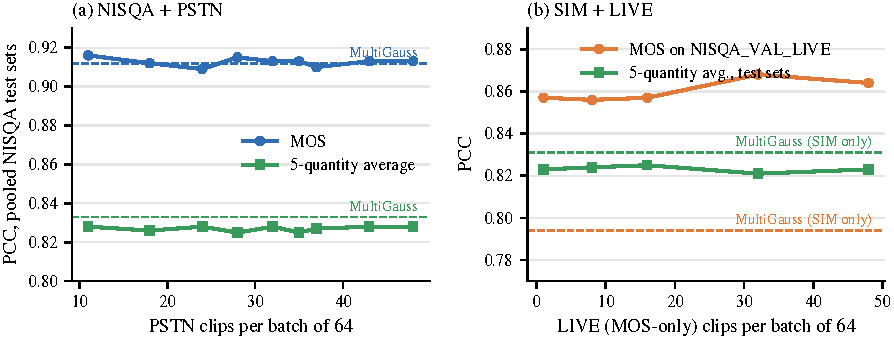
\includegraphics[width=\textwidth]{figures/thesis/batch_ratio.pdf}
  \caption{Effect of the share of MOS-only clips in a 64-clip training batch. (a) Experiment~A setting: NISQA with PSTN, evaluated on the pooled NISQA test sets. (b) Experiment~B setting: NISQA\_TRAIN\_SIM with NISQA\_TRAIN\_LIVE as MOS-only data. Dashed lines show MultiGauss. Mean of three runs at each point.}
  \label{fig:batchRatio}
\end{figure}

\subsection{Equal amounts of data}

Two further checks were made in the Experiment~B setting, to rule out simple explanations for the results in Section~\ref{sec:resultsExpB}. First, the first stage of the two-stage model sees only 32 fully labelled clips per step, while MultiGauss sees 64. With 64 SIM and 64 LIVE clips per step, so that both models see the same number of fully labelled clips, the results were practically unchanged: the average over the five quantities on the test sets was 0.818 (MultiGauss 0.831), and the MOS gain on NISQA\_VAL\_LIVE remained (+0.072$^{*}$).

Second, in the main setting the 1\,020 LIVE clips are repeated about ten times more often than the 10\,000 SIM clips. With equal pools of 1\,020 SIM and 1\,020 LIVE clips, compared with MultiGauss trained on the same 1\,020 SIM clips, the pattern was the same. MOS improved on NISQA\_VAL\_LIVE (0.861 against 0.772, $+0.089^{*}$) and on the pooled validation sets ($+0.008^{*}$), while the average over the five quantities on the test sets did not improve (0.784 against 0.792, not significant).

\subsection{Amount of multidimensional data}

The low-data study tests the situation that motivates this thesis: little multidimensional data, with MOS-only data to make up for it. Out of a budget of 500 clips, a varying number came from NISQA with all five labels and the rest from PSTN with MOS only. MultiGauss was trained on exactly the same NISQA clips, but cannot use the PSTN clips. Figure~\ref{fig:lowData} shows the results.

With the same fully labelled clips, the two-stage model predicted MOS better than MultiGauss at six of the seven data sizes, by 0.014 to 0.027 PCC (Figure~\ref{fig:lowData}a). The gain is largest when the multidimensional data is scarcest: with only 100 NISQA clips, the two-stage model reached 0.855 against 0.828. However, the run-to-run variation at this data size is large (standard deviation 0.01--0.04), so the individual differences are uncertain. The dimension predictions did not benefit (Figure~\ref{fig:lowData}b). The average over the five quantities was lower than MultiGauss at every data size, by 0.009 to 0.037, because the four dimensions were predicted worse.

A related study kept 500 NISQA clips fixed and added 200 to 1\,000 PSTN clips. MOS PCC rose from 0.871 to 0.880, compared with 0.864 for MultiGauss on the same 500 NISQA clips. The average over the five quantities stayed between 0.754 and 0.763, again below MultiGauss (0.773).

\begin{figure}[!ht]
  \centering
  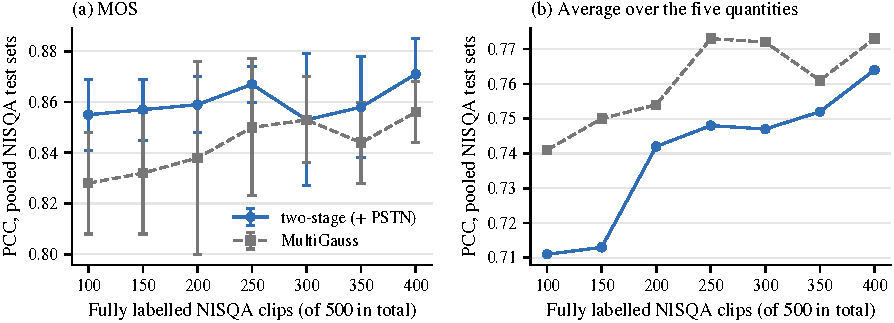
\includegraphics[width=\textwidth]{figures/thesis/low_data.pdf}
  \caption{Low-data study. Both models are trained on the same fully labelled NISQA clips; the two-stage model additionally receives PSTN clips with MOS labels, up to a total of 500 clips. PCC on the pooled NISQA test sets, mean of three runs; error bars in (a) show the standard deviation over runs.}
  \label{fig:lowData}
\end{figure}

\subsection{XLS-R layer}

Table~\ref{tab:sslLayer} compares features from three XLS-R layers, each at three batch ratios (single runs). Layer~12 gave the best MOS prediction on the NISQA test sets at every ratio, and its PSTN results were on par with the deeper layers. Layer~12, which is also the layer used by MultiGauss~\cite{cumlin_multigauss_2025}, was therefore kept.

\begin{table}[!ht]
  \centering
  \caption{MOS PCC for features from three XLS-R layers, at three shares of NISQA clips in the batch, on the pooled NISQA test sets and on PSTN\_VAL2K. Single training runs.}
  \label{tab:sslLayer}
  \setlength{\tabcolsep}{4pt}
  \begin{adjustbox}{max width=\textwidth}
  \begin{tabular}{lcccccc}
    \toprule
     & \multicolumn{3}{c}{NISQA test sets} & \multicolumn{3}{c}{PSTN\_VAL2K} \\
    \cmidrule(lr){2-4}\cmidrule(lr){5-7}
    NISQA share of batch & 20\,\% & 50\,\% & 80\,\% & 20\,\% & 50\,\% & 80\,\% \\
    \midrule
    Layer 12 & \textbf{0.909} & \textbf{0.896} & \textbf{0.900} & \textbf{0.804} & 0.783 & 0.803 \\
    Layer 22 & 0.880 & 0.868 & 0.877 & 0.779 & \textbf{0.808} & 0.805 \\
    Layer 32 & 0.872 & 0.871 & 0.858 & 0.788 & 0.793 & \textbf{0.810} \\
    \bottomrule
  \end{tabular}
  \end{adjustbox}
\end{table}

\subsection{Summary of the design studies}

The final two-stage model uses XLS-R layer~12, a MOS stage that receives both the encoded features and the dimension values, teacher forcing, and a balanced batch of 32 fully labelled and 32 MOS-only clips. None of the design choices studied had a large effect. Across all studies, the same pattern appears: the MOS-only data helps MOS, but not the four dimensions.

\section{Experiment A: adding a separate MOS-only corpus}
\label{sec:resultsExpA}

Table~\ref{tab:expAMix} shows MOS prediction on the combined set of 2\,000 NISQA validation clips and 2\,000 PSTN validation clips. On the combined set, the two-stage model reached a PCC of 0.882, against 0.846 for MultiGauss, a significant improvement of 0.036. It also predicted the PSTN clips significantly better (0.818 against 0.801). On the NISQA half, MultiGauss was slightly better (0.923 against 0.919); the difference of 0.004 is small but significant.

The combined set shows a larger gain than either half on its own. This means that a large part of the improvement comes from placing clips from the two corpora on a more consistent common scale, so that a PSTN clip and a NISQA clip with the same true quality get similar predictions. MultiGauss, which never saw PSTN data, ranks the clips within each corpus almost as well, but places the two corpora less consistently relative to each other.

\begin{table}[!ht]
  \centering
  \caption{Experiment A: MOS prediction on the combined NISQA and PSTN validation set, and on each half. $\Delta$ is the two-stage model minus MultiGauss.}
  \label{tab:expAMix}
  \begin{adjustbox}{max width=\textwidth}
  \begin{tabular}{lccc}
    \toprule
     & Combined (4\,000) & NISQA half (2\,000) & PSTN half (2\,000) \\
    \midrule
    \multicolumn{4}{l}{\emph{PCC}} \\
    Two-stage model & \textbf{0.882} & 0.919 & \textbf{0.818} \\
    MultiGauss      & 0.846 & \textbf{0.923} & 0.801 \\
    $\Delta$        & $+0.036^{*}$ & $-0.004^{*}$ & $+0.017^{*}$ \\
    \midrule
    \multicolumn{4}{l}{\emph{RMSE}} \\
    Two-stage model & 0.718 & 0.730 & 0.707 \\
    MultiGauss      & \textbf{0.592} & \textbf{0.495} & \textbf{0.674} \\
    \bottomrule
  \end{tabular}
  \end{adjustbox}
\end{table}

Table~\ref{tab:expANisqaVal} shows all five quantities on the NISQA validation sets. The two models are tied: every difference is 0.005 or smaller and none is significant. Adding PSTN therefore did not improve the four dimensions, but did not harm them either.

\begin{table}[!ht]
  \centering
  \caption{Experiment A: PCC on the pooled NISQA validation sets (2\,700 clips). None of the differences is significant.}
  \label{tab:expANisqaVal}
  \setlength{\tabcolsep}{4pt}
  \begin{adjustbox}{max width=\textwidth}
  \begin{tabular}{lcccccc}
    \toprule
     & MOS & NOI & COL & DIS & LOUD & Avg. \\
    \midrule
    Two-stage model & 0.918 & 0.870 & 0.855 & 0.863 & 0.818 & 0.865 \\
    MultiGauss      & 0.923 & 0.872 & 0.858 & 0.867 & 0.823 & 0.868 \\
    \bottomrule
  \end{tabular}
  \end{adjustbox}
\end{table}

\paragraph{Corpora not seen in training.} The models were also evaluated on two MOS-only corpora that neither of them was trained on: BVCC~\cite{cooper_ssw_2021}, with synthetic speech, and TCD-VoIP~\cite{harte_tcdvoip_2015}, with \gls{VoIP} degradations. On a combined set of 383 clips each from NISQA, PSTN, BVCC and TCD-VoIP, the two-stage model reached a MOS PCC of 0.856 against 0.813 for MultiGauss, a significant improvement. On each unseen corpus on its own, however, it did not do better: on BVCC its PCC was 0.835 against 0.843 (not significant), and on TCD-VoIP 0.871 against 0.887 (significant). The gain on the combined set therefore again comes mainly from a more consistent scale across corpora, not from ranking the clips within a new corpus better.

\section{Experiment B: a MOS-only subset of the same corpus}
\label{sec:resultsExpB}

In Experiment~B, the two-stage model was trained on NISQA\_TRAIN\_SIM with all five labels and NISQA\_TRAIN\_LIVE with MOS only, and compared with MultiGauss trained on NISQA\_TRAIN\_SIM only. Table~\ref{tab:expB} shows the results.

\begin{table}[!ht]
  \centering
  \caption{Experiment B: PCC of the two-stage model (SIM with all labels and LIVE with MOS only) and MultiGauss (SIM only). $\Delta$ is the two-stage model minus MultiGauss.}
  \label{tab:expB}
  \setlength{\tabcolsep}{4pt}
  \begin{adjustbox}{max width=\textwidth}
  \begin{tabular}{llcccccc}
    \toprule
    Evaluation set & & MOS & NOI & COL & DIS & LOUD & Avg. \\
    \midrule
    NISQA\_VAL\_LIVE & Two-stage & 0.868 & 0.641 & 0.549 & 0.571 & 0.688 & 0.663 \\
    (200 clips)      & MultiGauss & 0.794 & 0.669 & 0.536 & 0.604 & 0.585 & 0.638 \\
                     & $\Delta$ & $+0.073^{*}$ & $-0.028$ & $+0.013$ & $-0.034$ & $+0.102^{*}$ & $+0.026$ \\
    \midrule
    NISQA\_VAL\_SIM  & Two-stage & 0.918 & 0.869 & 0.850 & 0.862 & 0.789 & 0.858 \\
    (2\,500 clips)   & MultiGauss & 0.920 & 0.878 & 0.853 & 0.875 & 0.790 & 0.863 \\
                     & $\Delta$ & $-0.002$ & $-0.009^{*}$ & $-0.004$ & $-0.013^{*}$ & $-0.002$ & $-0.006^{*}$ \\
    \midrule
    Test sets, pooled & Two-stage & 0.906 & 0.843 & 0.876 & 0.872 & 0.606 & 0.821 \\
    (712 clips)       & MultiGauss & 0.913 & 0.840 & 0.877 & 0.883 & 0.640 & 0.831 \\
                      & $\Delta$ & $-0.006$ & $+0.003$ & $-0.001$ & $-0.012$ & $-0.034^{*}$ & $-0.010^{*}$ \\
    \bottomrule
  \end{tabular}
  \end{adjustbox}
\end{table}

On the live validation clips, which come from the same domain as the MOS-only training data, the two-stage model predicted MOS clearly better than MultiGauss ($+0.073^{*}$). Loudness also improved there ($+0.102^{*}$). The other three dimensions did not improve, and none of the differences in them is significant. On the simulated validation clips the two-stage model was slightly worse, mainly in noisiness and discontinuity. On the held-out test sets, MOS was not significantly different, but the average over the five quantities was significantly lower ($-0.010^{*}$), mostly because of loudness ($-0.034^{*}$). Looking at the three test sets separately, the average was lower on all three (by 0.012 on FOR, 0.015 on P501 and 0.012 on LIVETALK), significantly so only on P501.

In short, the MOS-only LIVE data improved MOS prediction on live speech, the domain the data came from, but it did not improve the four dimensions in general.

\section{Comparison with the masked-loss baseline}
\label{sec:resultsMasked}

Figure~\ref{fig:expBDeltas} and Table~\ref{tab:masked} compare the two-stage model with MultiGauss trained on the same SIM and LIVE data, using the masked loss of Section~\ref{sec:nanBaseline}. Both are shown relative to MultiGauss trained on SIM only.

\begin{figure}[!ht]
  \centering
  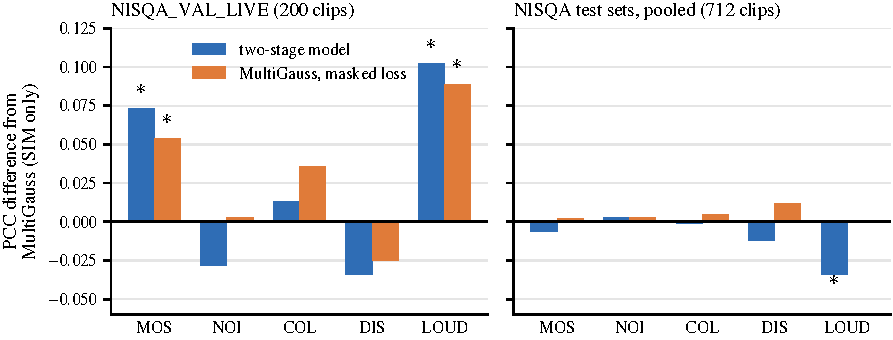
\includegraphics[width=\textwidth]{figures/thesis/exp_b_deltas.pdf}
  \caption{Experiment B: PCC of the two-stage model and of MultiGauss with the masked loss, both trained on SIM with all labels and LIVE with MOS only, relative to MultiGauss trained on SIM only. $^{*}$: significant difference from MultiGauss (SIM only).}
  \label{fig:expBDeltas}
\end{figure}

\begin{table}[!ht]
  \centering
  \caption{Experiment B: the two-stage model compared with MultiGauss with the masked loss, trained on the same data. $\Delta$ is the two-stage model minus the masked-loss model.}
  \label{tab:masked}
  \setlength{\tabcolsep}{4pt}
  \begin{adjustbox}{max width=\textwidth}
  \begin{tabular}{llcccccc}
    \toprule
    Evaluation set & & MOS & NOI & COL & DIS & LOUD & Avg. \\
    \midrule
    NISQA\_VAL\_LIVE & Two-stage & 0.868 & 0.641 & 0.549 & 0.571 & 0.688 & 0.663 \\
                     & Masked loss & 0.848 & 0.672 & 0.572 & 0.579 & 0.674 & 0.669 \\
                     & $\Delta$ & $+0.020$ & $-0.031$ & $-0.023$ & $-0.008$ & $+0.014$ & $-0.006$ \\
    \midrule
    NISQA validation, & Two-stage & 0.919 & 0.858 & 0.851 & 0.853 & 0.810 & 0.858 \\
    pooled            & Masked loss & 0.921 & 0.872 & 0.858 & 0.867 & 0.813 & 0.866 \\
                      & $\Delta$ & $-0.002$ & $-0.014^{*}$ & $-0.007^{*}$ & $-0.014^{*}$ & $-0.003$ & $-0.008^{*}$ \\
    \midrule
    Test sets, pooled & Two-stage & 0.906 & 0.843 & 0.876 & 0.872 & 0.606 & 0.821 \\
                      & Masked loss & 0.914 & 0.844 & 0.882 & 0.895 & 0.640 & 0.835 \\
                      & $\Delta$ & $-0.008$ & $-0.001$ & $-0.006$ & $-0.023^{*}$ & $-0.034$ & $-0.014^{*}$ \\
    \bottomrule
  \end{tabular}
  \end{adjustbox}
\end{table}

The masked-loss model gained almost as much on live MOS as the two-stage model ($+0.054^{*}$ against $+0.073^{*}$ over MultiGauss on SIM only), and the remaining difference of 0.020 between them is not significant. It also gained on live loudness, as the two-stage model did. Unlike the two-stage model, however, it lost nothing on the other sets: on the test sets its average over the five quantities was 0.835, the same as MultiGauss on SIM only (0.831, not significant), and significantly higher than the two-stage model (0.821).

The benefit of the MOS-only data in Experiment~B is therefore available to a standard joint model with a masked loss, without the two-stage structure. The two-stage structure itself does not add to it, and costs some accuracy in the four dimensions.

\section{Hyperparameter tuning}
\label{sec:resultsTuning}

The two-stage model was tuned in the setting of Experiment~A, with every setting chosen on the NISQA validation sets. The learning rate and its schedule had little effect: the average PCC of the four dimensions on the validation sets ranged only from 0.847 to 0.854. Weight decay and stronger dropout did not improve the test results either. Two changes did help. The first was to select the checkpoint on the average PCC of the four dimensions on the validation sets, instead of on MOS alone. The second was to weight the dimension loss four times higher than the MOS losses, which gives the first stage a stronger training signal. Table~\ref{tab:tuning} compares the tuned model with the original recipe and with MultiGauss.

\begin{table}[!ht]
  \centering
  \caption{Hyperparameter tuning in the Experiment A setting: PCC on the pooled NISQA test sets and MOS PCC on PSTN\_VAL2K. The tuned model uses a learning rate of $3\times10^{-4}$ with a cosine schedule, a four times higher weight on the dimension loss, and checkpoint selection on the four dimensions.}
  \label{tab:tuning}
  \setlength{\tabcolsep}{4pt}
  \begin{adjustbox}{max width=\textwidth}
  \begin{tabular}{lccccccc}
    \toprule
     & MOS & NOI & COL & DIS & LOUD & Avg. & PSTN MOS \\
    \midrule
    Original recipe & 0.913 & 0.833 & 0.879 & 0.889 & 0.593 & 0.821 & \textbf{0.819} \\
    Tuned           & \textbf{0.917} & 0.842 & \textbf{0.894} & \textbf{0.901} & \textbf{0.646} & \textbf{0.840} & \textbf{0.819} \\
    MultiGauss      & 0.912 & \textbf{0.844} & 0.879 & 0.894 & 0.638 & 0.833 & 0.801 \\
    \bottomrule
  \end{tabular}
  \end{adjustbox}
\end{table}

Compared with the original recipe, the tuned model improved the average over the five quantities by 0.019$^{*}$, mostly through loudness ($+0.053^{*}$), without any loss in MOS. Compared with MultiGauss, it was now on par on the NISQA test sets: the average was 0.007 higher, which is not significant, and coloration was significantly better ($+0.015^{*}$). It kept the advantage on PSTN ($+0.018^{*}$). Tuning therefore closes the gap in the four dimensions that the original recipe has, but it does not produce a model that is clearly better than MultiGauss on NISQA. The tuned model was evaluated only in the Experiment~A setting.

\section{Absolute accuracy of the predictions}
\label{sec:resultsCalibration}

The tables above also show a consistent difference in RMSE. In every experiment, the MOS predictions of the two-stage model have a clearly higher RMSE than those of MultiGauss, even where the PCC is the same or higher: for example 0.82 against 0.47 on the test sets in Experiment~B, and 0.73 against 0.50 on the NISQA half of Experiment~A. Since PCC is unaffected by a constant shift and RMSE is not, this points to a systematic offset. Indeed, the two-stage model in Experiment~B overestimates MOS on the test sets by 0.70 on average, against about 0.19 for MultiGauss. When this mean offset is removed, the MOS RMSE of every model falls to between 0.42 and 0.44. In Experiment~A, the two-stage model likewise overestimates MOS on all four corpora of the combined set (by 0.49 on NISQA, 0.51 on PSTN, 0.96 on BVCC and 0.76 on TCD-VoIP). The two-stage model therefore ranks clips as well as MultiGauss, but its absolute values are shifted upwards. The four dimensions are much less affected: on the pooled test sets of Experiment~B, their RMSE is at most 0.05 higher than for MultiGauss.

\section{Reliability Analysis}
\label{sec:reliabilityAnalysis}

The variation between training runs was small for the main experiments: the standard deviation of the pooled test MOS PCC over three runs was typically 0.002--0.005, and up to about 0.01--0.02 for the dimensions. Differences of about 0.01 are therefore close to what training randomness alone can produce, which is why every comparison was tested for significance rather than judged from the means. The early project also showed how misleading a single run can be: in a three-run repetition of a study that was first run once, the dimension PCCs of the single run turned out to be 0.01--0.016 too high. The design studies that were run only once (the XLS-R layer and the first batch ratio study) should therefore be read as indicative. In the low-data studies, the variation between runs is larger (up to 0.04), because each run draws a different small subset of clips, and the individual differences there are uncertain.

\section{Validity Analysis}
\label{sec:validityAnalysis}

Several factors limit how far the results can be generalised. First, every model's checkpoint was selected on NISQA validation MOS, so all results on the NISQA validation sets are slightly optimistic. This affects the baselines and the two-stage model alike, and the test sets, which were never used for any choice, give the cleaner comparison. Second, in Experiment~A the baseline is the single published MultiGauss checkpoint, which was trained with an 8-second crop, while the two-stage model uses 10 seconds. The comparison therefore includes this small difference in input, and the significance test covers only the variation over clips for MultiGauss. Experiment~B avoids both issues, since all its models were trained in this thesis with the same pipeline and three runs each. Third, pooling several test sets mixes ranking within each set with consistency between sets. Results are therefore also reported per set where it matters. Finally, all conclusions are based on one multidimensional corpus (NISQA) and one main MOS-only training corpus (PSTN, or the live part of NISQA), and may differ for other corpora.

\cleardoublepage
\chapter{Discussion}
\label{ch:discussion}
\sweExpl{Diskussion\\
Förbättringsförslag?}
\generalExpl{This can be a separate chapter or a section in the previous chapter.}

\cleardoublepage
\chapter{Conclusions and Future work}
\label{ch:conclusionsAndFutureWork}
\sweExpl{Slutsats och framtida arbete}

\generalExpl{Add text to introduce the subsections of this chapter.}

\section{Conclusions}
\label{sec:conclusions}
\sweExpl{Slutsatser}
\engExpl{Describe the conclusions (reflect on the whole introduction given in Chapter 1).}


  
\engExpl{Discuss the positive effects and the drawbacks.\\
Describe the evaluation of the results of the degree project.\\
Did you meet your goals?\\
What insights have you gained?\\
What suggestions can you give to others working in this area?\\
If you had it to do again, what would you have done differently?}

\sweExpl{Uppfyllde du dina mål?\\
Vilka insikter har du fått?\\
Vilka förslag kan du ge till andra som arbetar inom detta område?
Om du skulle göra detta igen, vad skulle du ha gjort annorlunda?}

\section{Limitations}
\label{sec:limitations}
\sweExpl{Begränsande faktorer\\Vad gjorde du som begränsade dina ansträngningar? Vilka är begränsningarna i dina resultat?}
\engExpl{What did you find that limited your efforts? What are the limitations of your results?}


\section{Future work}
\label{sec:futureWork}
\sweExpl{Vad du har kvar ogjort?\\Vad är nästa självklara saker som ska göras?\\Vad tips kan du ge till nästa person som kommer att följa upp på ditt arbete?}
\engExpl{Describe valid future work that you or someone else could or should do.\\
Consider: What you have left undone? What are the next obvious things to be done? What hints can you give to the next person who is going to follow up on your work?}



Due to the breadth of the problem, only some of the initial goals have been
met. In these section we will focus on some of the remaining issues that
should be addressed in future work. ...

\subsection{What has been left undone?}
\label{what-has-been-left-undone}

The prototype does not address the third requirment, \ie a yearly unavailability of less than 3 minutes; this remains an open problem. ...

\subsubsection{Cost analysis}
\generalExpl{Example of a missing component}
The current prototype works, but the performance from a cost perspective makes this an impractical solution. Future work must reduce the cost of this solution; to do so, a cost analysis needs to first be done. ...

\subsubsection{Security}
\generalExpl{Example of a missing component}
A future research effort is needed to address the security holes that results from using a self-signed certificate. Page filling text mass. Page filling text mass. ...


\subsection{Next obvious things to be done}

In particular, the author of this thesis wishes to point out xxxxxx remains as a problem to be solved. Solving this problem is the next thing that should be done. ...

\section{Reflections}
\label{sec:reflections}
\sweExpl{Reflektioner}
\sweExpl{Vilka är de relevanta ekonomiska, sociala, miljömässiga och etiska aspekter av ditt arbete?}
\engExpl{What are the relevant economic, social,
  environmental, and ethical aspects of your work?
}



One of the most important results is the reduction in the amount of
energy required to process each packet while at the same time reducing the
time required to process each packet.

The thesis contributes to the UN Sustainable Development Goals numbers 1 and 9 by
xxxx. 




\noindent\rule{\textwidth}{0.4mm}
\engExpl{In the references, let Zotero or other tool fill this in for you. I suggest an extended version of the IEEE style, to include URLs, DOIs, ISBNs, etc., to make it easier for your reader to find them. This will make life easier for your opponents and examiner. \\IEEE Editorial Style Manual: \url{https://www.ieee.org/content/dam/ieee-org/ieee/web/org/conferences/style_references_manual.pdf}}
\sweExpl{Låt Zotero eller annat verktyg fylla i det här för dig. Jag föreslår en utökad version av IEEE stil - att inkludera webbadresser, DOI, ISBN osv. - för att göra det lättare för läsaren att hitta dem. Detta kommer att göra livet lättare för dina opponenter och examinator.}

\cleardoublepage
% Print the bibliography (and make it appear in the table of contents)
\renewcommand{\bibname}{References}


\iftoggle{biblatex}{
    %\typeout{Biblatex current language is \currentlang}
    \printbibliography[heading=bibintoc]
}{
    \phantomsection  % make it include a hyperref - see https://tex.stackexchange.com/a/98995
    \addcontentsline{toc}{chapter}{References}
    \bibliography{references}
}



\warningExpl{If you do not have an appendix, do not include the \textbackslash cleardoublepage command below; otherwise, the last page number in the metadata will be one too large.}
\cleardoublepage
\appendix
\renewcommand{\chaptermark}[1]{\markboth{Appendix \thechapter\relax:\thinspace\relax#1}{}}
\chapter{Training step of the two-stage model}
\label{app:trainingStep}

The listing below shows one training step of the two-stage model, corresponding to Equation~\eqref{eq:totalLoss}. It is taken from the training code used for the experiments, with code for options not used in this thesis removed. \texttt{labelled} is a batch of fully labelled clips and \texttt{mos\_only} a batch of MOS-only clips.

\begin{lstlisting}[language=Python, basicstyle=\ttfamily\footnotesize, breaklines=true, frame=single, columns=fullflexible]
def multivariate_gnll(means, targets, covariance, eps=1e-6):
    """Multivariate Gaussian negative log-likelihood (Stage 1).
    As in the MultiGauss code, the log-determinant is floored at eps."""
    log_det = torch.maximum(torch.logdet(covariance),
                            torch.tensor(eps, device=means.device))
    diff = (means - targets).unsqueeze(-1)
    mahalanobis = diff.transpose(1, 2) @ torch.inverse(covariance) @ diff
    return torch.mean(mahalanobis.squeeze() / 2 + log_det / 2)

def univariate_gnll(means, targets, variance, eps=1e-6):
    """Univariate Gaussian negative log-likelihood (Stage 2)."""
    variance = torch.clamp(variance.reshape(-1), min=eps)
    diff = means.reshape(-1) - targets.reshape(-1)
    return torch.mean(torch.log(2 * torch.pi * variance) / 2
                      + diff.pow(2) / (2 * variance))

def train_step(model, optimizer, labelled, mos_only):
    # Fully labelled clips: label columns are [mos, noi, col, dis, loud].
    features, labels = labelled
    mos_targets, dim_targets = labels[:, 0], labels[:, 1:5]

    encoded = model.projection_head.encode(features)       # shared encoder
    dim_means, dim_cov = model.projection_head.decode(encoded)  # Stage 1
    # Stage 2 with teacher forcing: true dimension values as input.
    mos_means, mos_var = model.mos_head(encoded, dim_targets)

    loss = multivariate_gnll(dim_means, dim_targets, dim_cov)  # dimensions
    loss = loss + univariate_gnll(mos_means, mos_targets, mos_var)  # MOS

    # MOS-only clips: full cascade, Stage 2 gets Stage 1's predictions.
    # The predictions are not detached, so this loss also trains Stage 1.
    features_m, mos_targets_m = mos_only
    (mos_means_m, mos_var_m), _ = model(features_m)
    loss = loss + univariate_gnll(mos_means_m, mos_targets_m, mos_var_m)

    optimizer.zero_grad()
    loss.backward()
    optimizer.step()
    return loss.item()
\end{lstlisting}

\cleardoublepage
\chapter{Supporting materials}
\label{sec:supportingMaterial}
\generalExpl{Here is a place to add supporting material that can help others build upon your work. You can include files as attachments to the PDF file or indirectly via URLs. Alternatively, consider adding supporting material uploaded as separate files in DiVA.}

% Attach the BibTeX for your references to make it easy for a reader to find and use them
The BibTeX references used in this thesis are attached. \attachfile[description={references.bib}]{references.bib}

% Attach source code file(s) or add a URL to the github or other repository
Some source code relevant to this project can be found at \url{https://github.com/gqmaguirejr/E-learning} and \url{https://github.com/gqmaguirejr/Canvas-tools}.

Your reader can access the attached (embedded) files using a PDF tool such as Adobe Acrobat Reader using the paperclip icon in the left menu, as shown in \Cref{fig:PDFreaderPaperclipExample} or by right-clicking on the push-pin icon in the PDF file and then using the menu to save the embedded file as shown in \Cref{fig:PDFreaderPushpinExample}.

An argument for including supporting material in the PDF file is that it will be available to anyone who has a copy of the PDF file. As a result, they do not have to look elsewhere for this material. This comes at the cost of a larger PDF file. However, the embedded files are encoded into a compressed stream within the PDF file; thus, reducing the number of additional bytes. For example, the references.bib file that was used in this example is \SI{10617}{\byte} in size but only occupies \SI{4261}{\byte} in the PDF file.

\warningExpl{DiVA is limited to $\approx$\SI{1}{\giga\byte} for each supporting file. If you have very large amounts of supporting material, you will probably want to use one of the data repositories. For additional help with this, contact KTH Library via 
\href{mailto:researchdata@kth.se}{researchdata@kth.se}.\\As of Spring 2024, there are plans to migrate this supporting data from DiVA to a research data repository.
}

\begin{figure}[!ht]
  \begin{center}
    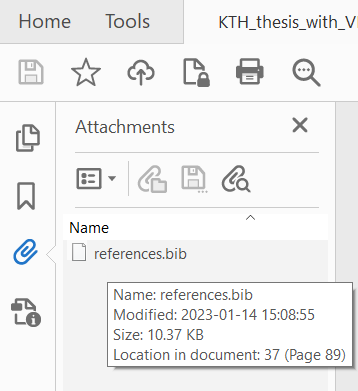
\includegraphics[width=0.50\textwidth]{README_notes/pdf-viewer-attached-files.png}
  \end{center}
  \caption{Adobe Acrobat Reader using the paperclip icon for the attached references.bib file}
  \label{fig:PDFreaderPaperclipExample}
\end{figure}
\FloatBarrier

\begin{figure}[!ht]
  \begin{center}
    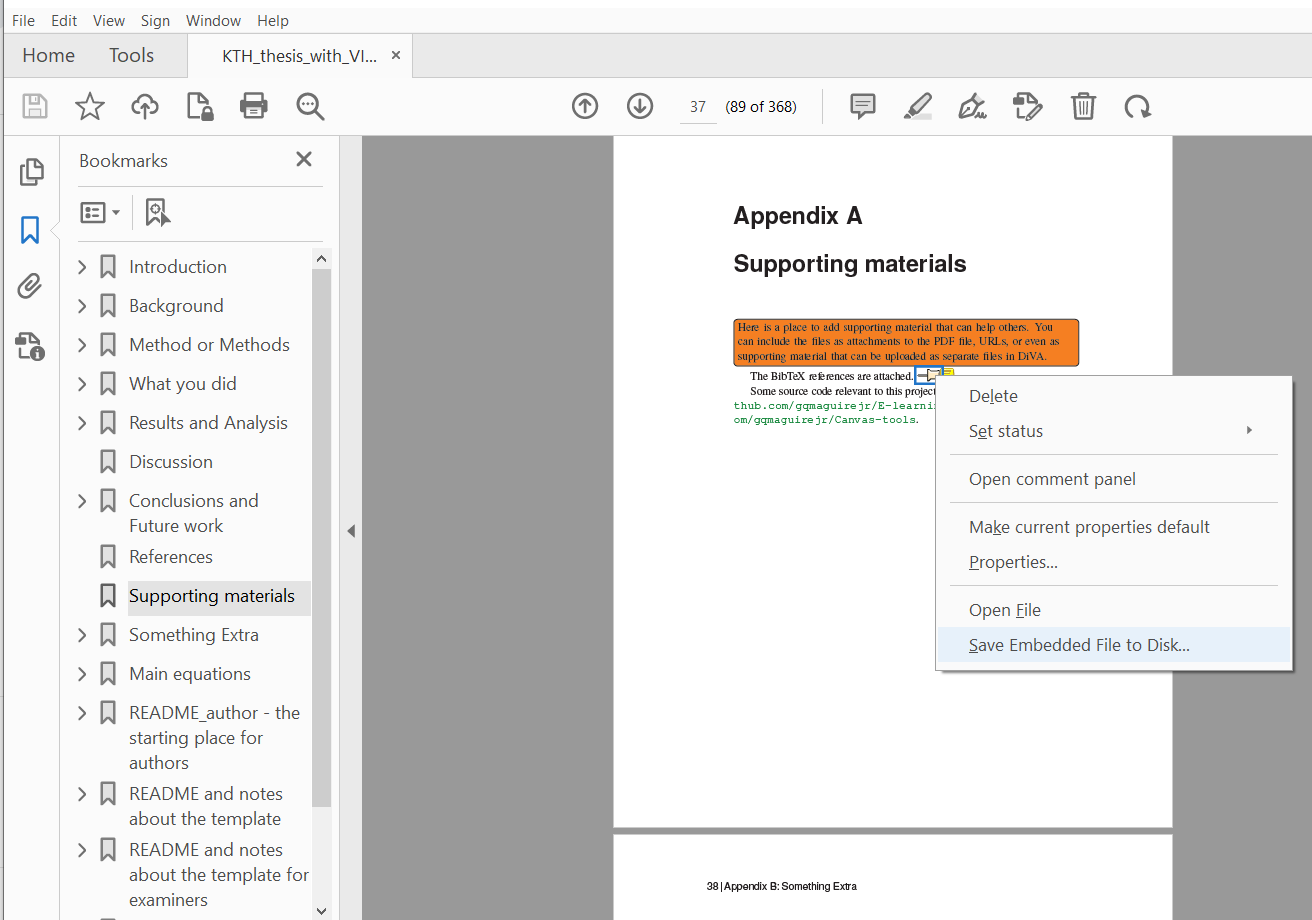
\includegraphics[width=0.99\textwidth]{README_notes/Bib-save-embedded-example.png}
  \end{center}
  \caption{Adobe Acrobat Reader after right-clicking on the push-pin icon for the attached references.bib file}
  \label{fig:PDFreaderPushpinExample}
\end{figure}
\FloatBarrier
\cleardoublepage

\chapter{Something Extra}
\sweExpl{svensk: Extra Material som Bilaga}

\section{Just for testing KTH colors}
\iftoggle{digitaloutput}{
    \textbf{You have selected to optimize for digital output}
}{
    \textbf{You have selected to optimize for print output}
}

\begin{itemize}[noitemsep]
    \item Primary color
    \begin{itemize}
    \item \textcolor{kth-blue}{kth-blue \iftoggle{digitaloutput}{
    actually Deep sea
    }{}} {\color{kth-blue} \rule{0.3\linewidth}{1mm} }\\

    \item \textcolor{kth-blue80}{kth-blue80} {\color{kth-blue80} \rule{0.3\linewidth}{1mm} }\\
\end{itemize}

\item  Secondary colors
\begin{itemize}[noitemsep]
    \item \textcolor{kth-lightblue}{kth-lightblue \iftoggle{digitaloutput}{
    actually Stratosphere
    }{}} {\color{kth-lightblue} \rule{0.3\linewidth}{1mm} }\\

    \item \textcolor{kth-lightred}{kth-lightred \iftoggle{digitaloutput}{
    actually Fluorescence}{}} {\color{kth-lightred} \rule{0.3\linewidth}{1mm} }\\

    \item \textcolor{kth-lightred80}{kth-lightred80} {\color{kth-lightred80} \rule{0.3\linewidth}{1mm} }\\

    \item \textcolor{kth-lightgreen}{kth-lightgreen \iftoggle{digitaloutput}{
    actually Front-lawn}{}} {\color{kth-lightgreen} \rule{0.3\linewidth}{1mm} }\\

    \item \textcolor{kth-coolgray}{kth-coolgray \iftoggle{digitaloutput}{
    actually Office}{}} {\color{kth-coolgray} \rule{0.3\linewidth}{1mm} }\\

    \item \textcolor{kth-coolgray80}{kth-coolgray80} {\color{kth-coolgray80} \rule{0.3\linewidth}{1mm} }
\end{itemize}
\end{itemize}

\textcolor{black}{black} {\color{black} \rule{\linewidth}{1mm} }

% Include an example of using nomenclature
\ifnomenclature
    \cleardoublepage
    \chapter{Main equations}
    \label{ch:NomenclatureExamples}
    This appendix gives some examples of equations that are used throughout this thesis.
    \section{A simple example}
    The following example is adapted from Figure 1 of the documentation for the package nomencl (\url{https://ctan.org/pkg/nomencl}).
    \begin{equation}\label{eq:mainEq}
    a=\frac{N}{A}
    \end{equation}
    \nomenclature{$a$}{The number of angels per unit area\nomrefeq}%       %% include the equation number in the list
    \nomenclature{$N$}{The number of angels per needle point\nomrefpage}%  %% include the page number in the list
    \nomenclature{$A$}{The area of the needle point}%
    The equation $\sigma = m a$%
    \nomenclature{$\sigma$}{The total mass of angels per unit area\nomrefeqpage}%
    \nomenclature{$m$}{The mass of one angel}
follows easily from \Cref{eq:mainEq}.

    \section{An even simpler example}
    The formula for the diameter of a circle is shown in \Cref{eq:secondEq} area of a circle in \cref{eq:thirdEq}.
    \begin{equation}\label{eq:secondEq}
    D_{circle}=2\pi r
    \end{equation}
    \nomenclature{$D_{circle}$}{The diameter of a circle\nomrefeqpage}%
    \nomenclature{$r$}{The radius of a circle\nomrefeqpage}%

    \begin{equation}\label{eq:thirdEq}
    A_{circle}=\pi r^2
    \end{equation}
    \nomenclature{$A_{circle}$}{The area of a circle\nomrefeqpage}%

    Some more text that refers to \eqref{eq:thirdEq}.
\fi  %% end of nomenclature example

\cleardoublepage
% Information for authors
%\documentclass[examplethesis.tex]{subfiles}

\begin{document}
\ifxeorlua
\lstdefinestyle{latexExampleForAuthors}{
language=[LaTeX]{TeX},
    breaklines=true,
    postbreak=\mbox{\textcolor{red}{$\hookrightarrow$}\space},
    basicstyle=\small\tt,
    keywordstyle=\color{blue}\sf,
    identifierstyle=\color{magenta},
    commentstyle=\color{cyan},
    backgroundcolor=\color{yellow!15},
    extendedchars=true,
    inputencoding=utf8,
    tabsize=2,
    columns=flexible,
    morekeywords={subtitle, alttitle, altsubtitle, hostcompany, courseCycle,
      courseCode, courseCredits, programcode, degreeName, subjectArea,
      nationalsubjectcategories, todo, ifbiblatex, subsection}
}
\else
\lstdefinestyle{latexExampleForAuthors}{
language=[LaTeX]{TeX},
    breaklines=true,
    postbreak=\mbox{\textcolor{red}{$\hookrightarrow$}\space},
    basicstyle=\small\tt,
    keywordstyle=\color{blue}\sf,
    identifierstyle=\color{magenta},
    commentstyle=\color{cyan},
    backgroundcolor=\color{yellow!15},
    extendedchars=false,
    inputencoding=utf8,
    tabsize=2,
    columns=flexible,
    morekeywords={subtitle, alttitle, altsubtitle, hostcompany, courseCycle,
      courseCode, courseCredits, programcode, degreeName, subjectArea,
      nationalsubjectcategories, todo, ifbiblatex, subsection},
% Support for Swedish, German and Portuguese umlauts
  literate=%
  {Ö}{{\"O}}1
  {Ä}{{\"A}}1
  {Å}{{\AA{}}}1
  {Ü}{{\"U}}1
  {ß}{{\ss}}1
  {ü}{{\"u}}1
  {ö}{{\"o}}1
  {ä}{{\"a}}1
  {å}{{\aa{}}}1
  {á}{{\'a}}1
  {ã}{{\~a}}1
  {é}{{\'e}}1
  {è}{{\`e}}1
  {€}{\euro}1%
  {’}{{\char13}}1
  {-}{{\textendash}}1
  {–}{{\textendash}}1
  {…}{{\ldots}}1,
}
\fi


\chapter{README\_author - the starting place for authors}
\label{ch:READMEauthor}

This chapter describes the thesis template that I (Gerald Q. Maguire Jr.) have developed for use at KTH Royal Institute of Technology (KTH). It is important to note that the template is \textbf{not prescriptive}, as not every thesis will have all of the parts that the template shows. However, if there is something that you decide to leave out, you should make a conscious decision to do so and you should consider the impact this may have on your thesis being approved by the examiner.

Fundamental to the design of the template are several key factors:
\begin{itemize}
    \item Helping students be successful in their degree project,
    \item Helping students produce a high-quality thesis, and
    \item Supporting all of the (relevant) phases of the degree project process.
\end{itemize}

\noindent\textbf{This document is a work in progress.}


\section{Advice for Author or Authors}
\label{sec:authors}
One of the hardest problems an author faces is getting started writing, \ie the blank sheet of paper -- empty file barrier. The template provides a \mbox{non-blank} starting point; hence, avoiding the blank paper barrier. Additionally, the template provides some initial structure, basically, an Introduction, Methods, Results, and Discussion (IMRAD) structure, so that there are hints of where to place material. Moreover, there are places (and notes) about material that the student should consider adding; for example, the ``required reflections'' section in the final chapter.

The template (located in the file \texttt{examplethesis.tex}) also provides some examples of commonly occurring types of content, so that one can easily find examples of how to include a figure, table, code listing, \etc. These examples are not meant to be exhaustive and quite often the student will probably need to learn new \LaTeX\  commands in the course of writing their thesis.

As an author, the first step is to configure the \LaTeX\  engine that you will use to process the files - see \Cref{sec:latexEngine}. The second step will be to configure the template - see \Cref{sec:authorConfigs}. The third step will be to make sure that the information about you, your supervisor(s), and the examiner are correct in the file \texttt{custom\_configuration.tex} - this information uses the macros described in \Cref{sec:authorMacros}. Now that you have a lot of the administrative details taken care of it is time to start to write - see \Cref{sec:startingToWrite}.

Note that if you are using Overleaf:
\begin{description}
    \item[Make your own copy of the template]
    If you have opened the template from a URL, in the upper left-hand corner, click on \textbf{Menu}. Then select \textbf{Copy Project} - this will give you your own private copy.

\item[Use a helpful project name]
    I suggest you include your name in the project name so that when you share it with your supervisor(s) and examiner, they will know it is your project. 
\item[Invite your supervisor(s) and examiner to your project] 
    You can invite your supervisor(s) and examiner to your project and they can directly comment on and correct your drafts.
\item[Log in to Overleaf with your KTH account] 
If you log in to Overleaf with your KTH account, you get a version of Overleaf that lets you turn on ``Track changes'' which is very useful (particularly if you have invited your supervisor(s) and examiner to join your project). It also gives you a bit more of a time budget to compile (which can be useful if you have a lot of Tikz figures or other things that take a lot of time for the LaTeX engine to render).
\end{description}

.


If you have more detailed questions about the template itself - 
\iflabelexists{ch:READMEnotes}{see \Cref{ch:READMEnotes}.}
{You have to include the \texttt{README\_notes/README\_notes.tex} file when compiling.}

\section{Author configuration of the \LaTeX\  engine}
\label{sec:latexEngine}
The template should work with \textsc{pdfLaTeX}, \XeLaTeX, and \LuaLaTeX.  If you are using Overleaf, I strongly recommend using \XeLaTeX\ ---  as this will get the \texttt{Arial} fonts correct for the KTH cover. If you are running the compiler on your local machine and you use \XeLaTeX\  \textbf{and} you have \texttt{Arial} as a system font, then it will be able to use it. Similarly, for \LuaLaTeX. For \textsc{pdfLaTeX} I have used \textbackslash fontfamily{helvet}, \ie Helvetica, as it is a sans serif font.

One student reported problems with \textsc{fontspec} not loading the fonts properly when running locally with macOS 12.4, TeXLive 2022, LaTeX Workshop on VS Code, and \XeLaTeX\  - the solution is described at \url{https://tug.org/TUGboat/tb39-2/tb122robertson-fontspec.pdf}.

If you are using Overleaf, it is easy to select the compiler (\ie \TeX\ engine) by using the drop-down menu, as shown in \Cref{fig:selectingTeXEngine}.
\begin{figure}[!ht]
  \begin{center}
    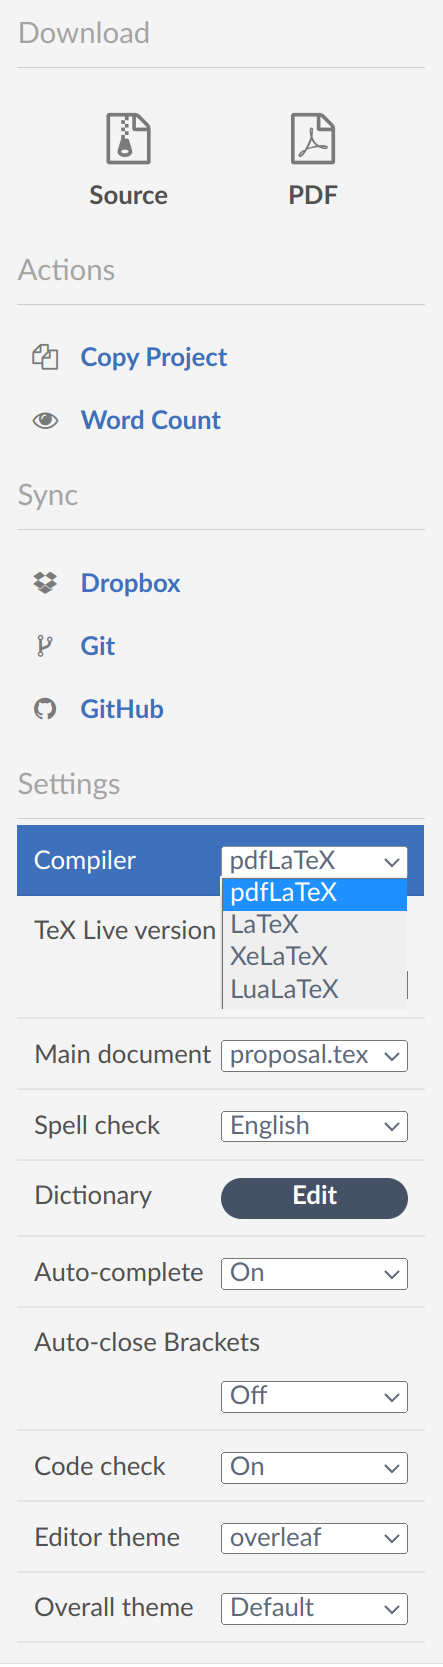
\includegraphics[width=0.40\textwidth]{README_notes/selecting-engine-in-overleaf.png}
  \end{center}
  \caption{Selecting a compiler (\ie TeX engine) in Overleaf}
  \label{fig:selectingTeXEngine}
\end{figure}
\FloatBarrier


\section{Author configuration of the template}
\label{sec:authorConfigs}
The template is designed to handle a thesis written in English or Swedish.
You can set the default language to `english' or `swedish' by passing an option to the documentclass. Note that the language option is written in all lowercase letters; for example, to set the document's language to English:
\begin{lstlisting}[style=latexExampleForAuthors]
\documentclass[english]{kththesis}
\end{lstlisting}

To set the document's language to Swedish (uncomment the following line):
\begin{lstlisting}[style=latexExampleForAuthors]
\documentclass[swedish]{kththesis}
\end{lstlisting}

The language option `swedish' sets the conditional \texttt{\textbackslash ifinswedish} to true.  Among many other things, this conditional is used to configure the KTH cover and the title page to use the chosen language.

The two most common bibliographic engines are supported, \ie BibTeX and BibLaTeX. To set the language to English and use the bibliographic engine to BibTeX you would say:
\begin{lstlisting}[style=latexExampleForAuthors]
\documentclass[english, bibtex]{kththesis}
\end{lstlisting}
To set the language to Swedish and use the bibliographic engine to BibLaTeX you would say:
\begin{lstlisting}[style=latexExampleForAuthors]
\documentclass[swedish, biblatex]{kththesis}
\end{lstlisting}

The above illustrates that you can pass multiple options to the document class separated by commas. Also, note that the options were passed as all lowercase letters.

You can, of course, also modify the formatting of the citations and bibliography. See for example the following code snippet:

\begin{lstlisting}[style=latexExampleForAuthors]
\ifbiblatex
    %\usepackage[language=english,bibstyle=authoryear, citestyle=authoryear, maxbibnames=99]{biblatex}
    %\usepackage[style=numeric,sorting=none,backend=biber]{biblatex}
    \usepackage[bibstyle=authoryear,citestyle=authoryear, maxbibnames=99,language=english]{biblatex}
    % alternatively you might use another style, such as IEEE
    %\usepackage[style=ieee]{biblatex}
    \addbibresource{references.bib}
    %\DeclareLanguageMapping{norsk}{norwegian}
\else
    % The line(s) below are for BibTeX
    \bibliographystyle{bibstyle/myIEEEtran}
    %\bibliographystyle{apalike}
\fi
\end{lstlisting}

To optimize for digital output (this changes the color palette) add the option: \texttt{digitaloutput}. There are also options for A4 or G6 paper: \texttt{a4paper} or \texttt{g5paper} (respectively). The is an option for \texttt{nomenclature}, to produce and refer to equations
\ifnomenclature
as shown in \Cref{ch:NomenclatureExamples}
\fi
.  Finally, there are options for a 1\textsuperscript{st} cycle thesis or 2\textsuperscript{nd} cycle thesis: \texttt{bachelor} and \texttt{master} (respectively); however, these two options are \textbf{not} currently used.

One of the first things that the author(s) will want to do is add the working title and subtitle to the thesis. This is done using the \textbackslash title, \textbackslash subtitle, \textbackslash alttitle, and \textbackslash altsubtitle macros as shown below:
\begin{lstlisting}[style=latexExampleForAuthors]
\title{This is the title in the language of the thesis}
\subtitle{A subtitle in the language of the thesis}

% give the alternative title - i.e., if the thesis is in English,
% then give a Swedish title
\alttitle{Detta är den svenska översättningen av titeln}
\altsubtitle{Detta är den svenska översättningen av undertiteln}
% alternative, if the thesis is in Swedish, then give an English title
%\alttitle{This is the English translation of the title}
%\altsubtitle{This is the English translation of the subtitle}   
\end{lstlisting}

Setting these values once and then using them in many places reduces the work to change them while at the same time ensuring consistency. 

\warningExpl{The issue of what characters can be placed in a title (subtitle, keywords, and abstracts) and how to enter them is a bit complex, but you should be able to achieve much of what you want - at the cost of some effort. Ultimately, the characters that will be placed into DiVA and LADOK must be Unicode, encoded using Unicode Transformation Format (UTF), specifically UTF-8. While DiVA utilizes HTML for these fields, allowing you to include some markup, LADOK does not support any markup.}

\warningExpl{If you have titles or subtitles that cannot be converted to pure Unicode (such as subscripts with capital letters or other symbols), you should also use the optional commands \texttt{\textbackslash titleInPlainText}, \texttt{\textbackslash subtitleInPlainText}, \texttt{\textbackslash alttitleInPlainText}, and \texttt{\textbackslash altsubtitleInPlainText} in your \texttt{custom\_configuration.tex} or \texttt{custom\_configuration\_plaintext.tex} files to provide versions of titles and subtitles that can be used with LADOK. Compiling \texttt{Generate\_titles\_in\_plain\_text.tex} with \textbf{\LuaLaTeX{}} will produce a file named \texttt{extra\_plaintext.tex} containing plain text versions of the \mbox{titles} and subtitles (both main and alternate). The reason that you have to compile using \LuaLaTeX{} is that I have used Lua code and \LuaLaTeX{} to compute the plain text strings. After you have compiled the file, you can follow the workflow to generate, download, edit and merge, and upload the \texttt{custom\_configuration\_plaintext.tex} file to your Overleaf project.}

Some additional configuration that the author(s) might do is to set the values of the macros related to the course cycle, course code, date of the thesis, number of credits, degree/exam name, subject area, and if the degree is done external to KTH to set the host information (see the file \textit{custom\_configuration.text}). Consider the snippet below for a student admitted to the ``Bachelor's Programme in Information and Communication Technology (TCOMK)'' program and enrolled in the degree project course ``IA150X Degree Project in Information and Communication Technology, First Cycle 15.0 credits'' and working at a company ``Företaget AB'':
\begin{lstlisting}[style=latexExampleForAuthors]
\hostcompany{Företaget AB} % Remove this line if the project was not done at a host company

\date{\today}

\courseCycle{1}
\courseCode{IA150X}
\courseCredits{15.0}

\programcode{TCOMK}
\degreeName{Bachelors degree}
% Note that the subject area for a Bachelor's thesis (Kandidatexamen)
% should be either Technology or Architecture
% If the thesis is in Swedish, these would be: teknik | arkitektur
% -- Note the use of lower case for the Swedish subject area
\subjectArea{Technology}
\end{lstlisting}

Note that in the above macros you have to give the English or Swedish names in the arguments to \textbackslash degreeName and \textbackslash subjectArea - as shown below:
\begin{lstlisting}[style=latexExampleForAuthors]
\degreeName{Kandidatexamen}
\subjectArea{teknik}
\end{lstlisting}

For a CDATE student enrolled in the course ``DA231X Degree Project in Computer Science and Engineering, Second Cycle 30.0 credits'', the cycle, program, course code, degree, and subject area information would be:
\begin{lstlisting}[style=latexExampleForAuthors]
\programcode{CDATE}
\courseCycle{2}
\courseCode{DA231X}
\courseCredits{30.0}
\degreeName{Degree of Master of Science in Engineering}
\subjectArea{Computer Science and Engineering}
\end{lstlisting}

The set of possible values for the English or Swedish names in the arguments to \textbackslash degreeName are:
\begin{lstlisting}[style=latexExampleForAuthors]
\degreeName{Higher Education Diploma}
\degreeName{Högskoleexamen}

\degreeName{Bachelors degree}
\degreeName{Kandidatexamen}

\degreeName{Master of Architecture}
\degreeName{Arkitektexamen}

\degreeName{Degree of Master of Science in Engineering}
\degreeName{Civilingenjörs}

\degreeName{Magister}
\degreeName{Magisterexamen}

\degreeName{Degree of Master of Science}
\degreeName{Masterexamen}

\degreeName{Master of Science in Engineering and Master of Arts in Education degree}
\degreeName{Civilingenjör och lärare examen}

\degreeName{Degree of Master of Science in Secondary Education}
\degreeName{Ämneslärarexamen}

\degreeName{Both}		# Degree Project in the Field of Technology <teknikområde> and the Main Field of Study <huvudområde>
\degreeName{Same}		# The case when the field of technology <teknikområde> and main field of study <huvudområde> are the same.
\end{lstlisting}

For the last two cases, the code compares the values of subjectArea and secondSubjectArea.

You can find a list of the program codes and school acronyms in the file:\linebreak[4] \texttt{lib/schools\_and\_programs.ins}.

There are a set of rules about what is to be displayed on the KTH cover. These can be found at \url{https://www.kth.se/social/group/sprakkommitten/page/omrade-for-examensarbete/}.

One of the reasons for many of the macros shown above and below is to collect the information that is needed to report the approved thesis in Digitala Vetenskapliga Arkivet (DiVA) and to report the title(s) and grade in \foreignlanguage{swedish}{Lokalt adb–baserat dokumentationssystem (LADOK)}.

National subject categories are a \textbf{required} field in the DiVA record. These categories follow a definition by \foreignlanguage{swedish}{SCB} (nowadays known as \foreignlanguage{swedish}{Statistikmyndigheten} or in English: Statistics Sweden) and HSV (\foreignlanguage{swedish}{Högskoleverket} - nowadays known as  \foreignlanguage{swedish}{Universitetskanslersämbetet (UK-ämbetet)} and \foreignlanguage{swedish}{Universitets- och högskolerådet (UHR)} or in English: Swedish Higher Education Authority and Swedish Council for Higher Education).
While these codes refer to research areas, these codes are also used in KTH to indicate the area of the thesis. The guidance that I received from the Linköping University library was that one should try to use 5-digit codes when possible. Some examples of these codes are shown in
\Cref{tab:examplesOfnNationalsubjectCategories}.
\begin{description}[leftmargin=!, labelwidth =\widthof{\texttt{\textbackslash nationalsubjectcategories\{\}}}]
\item [\texttt{\textbackslash nationalsubjectcategories\{\}}] comma-separated list of national subject category codes - each a 3 or 5 digit code
\end{description}

\Needspace*{2\baselineskip}
An example for a thesis in Computer Science and Computer Systems:
\begin{lstlisting}[style=latexExampleForAuthors]
\nationalsubjectcategories{10201, 10206}
\end{lstlisting}

You can find examples of the subjects and their codes at in \Cref{tab:examplesOfnNationalsubjectCategories}. The complete list can be found AT \url{https://www.scb.se/contentassets/3a12f556522d4bdc887c4838a37c7ec7/standard-for-svensk-indelning--av-forskningsamnen-2011-uppdaterad-aug-2016.pdf}\\
and\\
\url{https://www.scb.se/contentassets/10054f2ef27c437884e8cde0d38b9cc4/oversattningsnyckel-forskningsamnen.pdf}

You can also find them in \texttt{README\_notes/National\_Subject\_Categories.tex}. This file can be processed separately or included as an appendix by commenting out the begin and end comments around it near the end of the \texttt{examplethesis.tex} file. The full list is about 14 pages long.

\begin{table}[!ht]
  \begin{center}
    \caption{Examples of some national subject categories and their codes}
    \label{tab:examplesOfnNationalsubjectCategories}
    \begin{tabular}{p{0.85cm} L{6.2cm} L{6.2cm}} % <-- Alignments: 1st column left, 2nd middle, with vertical lines in between
      \textbf{Code}  & \textbf{Category (in Swedish)} & \textbf{Category (in English)} \\
      \hline
102 & \foreignlanguage{swedish}{Data- och informationsvetenskap (Datateknik)} &   Computer and Information Sciences \\
      \hline
10201 & \foreignlanguage{swedish}{Datavetenskap (datalogi)} & Computer Sciences \\
      \hline
10202 & \foreignlanguage{swedish}{Systemvetenskap, informationssystem och informatik} (\foreignlanguage{swedish}{samhällsvetenskaplig inriktning} under 50804) &
Information Systems (Social aspects to be 50804)\\
      \hline
10203 & \foreignlanguage{swedish}{Bioinformatik (beräkningsbiologi)} (\foreignlanguage{swedish}{tillämpningar} under 10610) & Bioinformatics (Computational Biology) (applications to be 10610) \\
      \hline
10204 & \foreignlanguage{swedish}{Människa-datorinteraktion (interaktionsdesign)} (\foreignlanguage{swedish}{Samhällsvetenskapliga aspekter} under 50803) & Human Computer Interaction (Social aspects to be 50803)\\
      \hline
10205 & \foreignlanguage{swedish}{Programvaruteknik} & Software Engineering \\
      \hline
10206 & \foreignlanguage{swedish}{Datorteknik} & Computer Engineering \\
      \hline
10207 & \foreignlanguage{swedish}{Datorseende och robotik (autonoma system) }& Computer Vision and Robotics (Autonomous Systems) \\
      \hline
10208 & \foreignlanguage{swedish}{Språkteknologi (språkvetenskaplig databehandling)} & Language Technology (Computational Linguistics) \\
      \hline
10209 & \foreignlanguage{swedish}{Medieteknik} & Media and Communication Technology \\
      \hline
10299 & \foreignlanguage{swedish}{Annan data- och informationsvetenskap} & Other Computer and Information Science \\
      \hline
      \hline
202   & \foreignlanguage{swedish}{Elektroteknik och elektronik} & Electrical Engineering, Electronic Engineering, Information Engineering \\
      \hline
20201 & \foreignlanguage{swedish}{Robotteknik och automation} & Robotics \\
      \hline
20202 & \foreignlanguage{swedish}{Reglerteknik} & Control Engineering \\
      \hline
20203 & \foreignlanguage{swedish}{Kommunikationssystem} & Communication Systems \\
      \hline
20204 & \foreignlanguage{swedish}{Telekommunikation} & Telecommunications \\
      \hline
20205 & \foreignlanguage{swedish}{Signalbehandling} & Signal Processing \\
      \hline
20206 & \foreignlanguage{swedish}{Datorsystem} & Computer Systems \\
      \hline
20207 & \foreignlanguage{swedish}{Inbäddad systemteknik} & Embedded Systems \\
      \hline
20299 & \foreignlanguage{swedish}{Annan elektroteknik och elektronik} & Other Electrical Engineering, Electronic Engineering, Information Engineering \\
      \hline
    \end{tabular}
  \end{center}
\end{table}


\FloatBarrier
\clearpage
\Needspace*{10\baselineskip}
\subsection{Setting the UN's Sustainable Development Goals (SDGs) information}
The UN's Sustainable Development Goals (SDGs) are a field in the DiVA record.
Some examples of these SDGs are shown in Table~\ref{tab:SDGcodes}.
\begin{description}[leftmargin=!, labelwidth =\widthof{\texttt{\textbackslash nationalsubjectcategories\{\}}}]
\item [\texttt{\textbackslash SDGs\{\}}] comma-separated list of SDG codes - each a numerical value
\end{description}

\Needspace*{2\baselineskip}
An example of a thesis supporting SDGs 8 and 9:
\begin{lstlisting}[style=latexExampleForAuthors]
\SDGs{8, 9}
\end{lstlisting}

%% UN's Sustainable Development Goals (SDGs)
% sdg1	eng: No poverty, swe: Ingen fattigdom
% sdg2	eng: Zero hunger, swe: Ingen hunger
% sdg3	eng: Good health and well-being, swe: God hälsa och välbefinnande
% sdg4	eng: Quality education, swe: God utbildning för alla
% sdg5	eng: Gender equality, swe: Jämställdhet
% sdg6	eng: Clean water and sanitation, swe: Rent vatten och sanitet för alla
% sdg7	eng: Affordable and clean energy, swe: Hållbar energi för alla
% sdg8	eng: Decent work and economic growth, swe: Anständiga arbetsvillkor och ekonomisk tillväxt
% sdg9	eng: Industry, innovation and infrastructure, swe: Hållbar industri, innovationer och infrastruktur
% sdg10	eng: Reduced inequalities, swe: Minskad ojämlikhet
% sdg11	eng: Sustainable cities and communities, swe: Hållbara städer och samhällen
% sdg12	eng: Responsible consumption and production, swe: Hållbar konsumtion och produktion
% sdg13	eng: Climate action, swe: Bekämpa klimatförändringarna
% sdg14	eng: Life below water, swe: Hav och marina resurser
% sdg15	eng: Life on land, swe: Ekosystem och biologisk mångfald
% sdg16	eng: Peace, justice and strong institutions, swe: Fredliga och inkluderande samhällen
% sdg17	eng: Partnerships for the goals, swe: Genomförande och globalt partnerskap

\begin{table}[!ht]
  \begin{center}
    \caption{UN's Sustainable Development Goals (SDGs)}
    \label{tab:SDGcodes}
    \begin{tabular}{p{0.85cm} L{6.0cm} L{6.0cm}} % <-- Alignments: 1st column left, 2nd middle, with vertical lines in between
      \textbf{SDG}  & \textbf{Category (in English)} & \textbf{Category (in Swedish)} \\
      \hline
1 & No poverty& \foreignlanguage{swedish}{Ingen fattigdom} \\ \hline
2 & Zero hunger& \foreignlanguage{swedish}{Ingen hunger} \\ \hline
3 & Good health and well-being& \foreignlanguage{swedish}{God hälsa och välbefinnande} \\ \hline
4 & Quality education& \foreignlanguage{swedish}{God utbildning för alla} \\ \hline
5 & Gender equality& \foreignlanguage{swedish}{Jämställdhet} \\ \hline
6 & Clean water and sanitation& \foreignlanguage{swedish}{Rent vatten och sanitet för alla} \\ \hline
7 & Affordable and clean energy& \foreignlanguage{swedish}{Hållbar energi för alla} \\ \hline
8 & Decent work and economic growth& \foreignlanguage{swedish}{Anständiga arbetsvillkor och ekonomisk tillväxt} \\ \hline
9 & Industry, innovation and infrastructure& \foreignlanguage{swedish}{Hållbar industri, innovationer och infrastruktur} \\ \hline
10 & Reduced inequalities& \foreignlanguage{swedish}{Minskad ojämlikhet} \\ \hline
11 & Sustainable cities and communities& \foreignlanguage{swedish}{Hållbara städer och samhällen} \\ \hline
12 & Responsible consumption and production& \foreignlanguage{swedish}{Hållbar konsumtion och produktion} \\ \hline
13 & Climate action& \foreignlanguage{swedish}{Bekämpa klimatförändringarna} \\ \hline
14 & Life below water& \foreignlanguage{swedish}{Hav och marina resurser} \\ \hline
15 & Life on land& \foreignlanguage{swedish}{Ekosystem och biologisk mångfald} \\ \hline
16 & Peace, justice and strong institutions& \foreignlanguage{swedish}{Fredliga och inkluderande samhällen} \\ \hline
17 & Partnerships for the goals& \foreignlanguage{swedish}{Genomförande och globalt partnerskap} \\ \hline
\end{tabular}
  \end{center}
\end{table}

\FloatBarrier

\section{Author macros}
\label{sec:authorMacros}
It is assumed that there can only be 1 or 2 authors. For many years now 2\textsuperscript{nd} cycle theses are expected to only have one author.

For the author or first author, there are a number of macros defined to store information about the author, so that it can later be used in multiple places -- for example, the KTH cover (produced with \texttt{\textbackslash kthcover)}, the title page (via \texttt{\textbackslash titlepage}, the ``For DIVA'' section at the end of the thesis (via
\texttt{\footnotesize\textbackslash divainfo\{pg:lastPageofPreface\}\{pg:lastPageofMainmatter\}}), and possibly a JavaScript Object Notation (JSON) file named \texttt{fordiva.json} produced as a by product of the \texttt{\textbackslash divainfo}. Note that the actual section name has DiVA set in all caps - which hopefully should not occur in the thesis! If the string DiVA set in all caps, does have to appear, then the section heading should be preceded by four euro signs and followed by four more euro signs (as is done in this document).

The author-related macros are:
\begin{description}[leftmargin=!, labelwidth =\widthof{\texttt{\textbackslash secondAuthorsFirstname\{\}}}]
\item [\texttt{\textbackslash authorsLastname\{\}}] the last name of the author\footnote{Note that the author's name can include a suffix such as ``, Jr.'' or `` Jr.'', i.e., the suffix can be separated with a comma or not -- as the author prefers to write their name.}

\item [\texttt{\textbackslash authorsFirstname\{\}}] the first name of the author

\item [\texttt{\textbackslash email\{\}}] the KTH e-mail address of the author

\item [\texttt{\textbackslash kthid\{\}}] the author's kthid, this generally starts with the string ·``u1'' and is a unique identifier for every KTH user.

% As per email from KTH Biblioteket on 2021-06-28 students cannot have an OrCiD reported for their degree project
\item [\texttt{\textbackslash authorsSchool\{\}}] the value is generally of the form:\linebreak[4] \texttt{\textbackslash schoolAcronym\{XXX\}}. The\linebreak[4] currently supported school acronyms are: ABE, CBH, EECS, ITM, and SCI. These are defined in the file\linebreak[4] \texttt{schools\_and\_programs.ins}. There is also a fake school XXX for use in the template.
\end{description}

If the first author is not in Stockholm, Sweden when the acknowledgements are written, then add that information via the macros described below.
This information will be used when generating the acknowledgements signature. The acknowledgements signature is the text at the end of the acknowledgements and it gives the place where the author(s) is/are when writing the acknowledgements and also gives the date and name(s).
\begin{description}[leftmargin=!, labelwidth =\widthof{\texttt{\textbackslash secondAuthorsFirstname\{\}}}]
\item [\texttt{\textbackslash authorCity\{A City\}}] specify the city

\item [\texttt{\textbackslash authorCountry\{A Country\}}] specify the country

\item [\texttt{\textbackslash authorCityCountryDate\{\}}] pass into this function the month and year for the acknowledgement. This can be a string such as January 2022 or it can be a \LaTeX\  expression, such as \textbackslash MONTH\textbackslash enspace\textbackslash the\textbackslash year.
\end{description}

If there is a second author and the place, month, and year are \textbf{all} the same, then specify the month and year for only the \textbf{first} author:
\begin{lstlisting}[style=latexExampleForAuthors]
\authorCityCountryDate{\MONTH\enspace\the\year}
\end{lstlisting}

If there is a second author and the place is different, then say:
\begin{lstlisting}[style=latexExampleForAuthors]
\authorCityCountryDate{}
\end{lstlisting}
%\clearpage

If there is a second author, the macros are:
\begin{description}[leftmargin=!, labelwidth =\widthof{\texttt{\textbackslash secondAuthorsFirstname\{\}}}]
\item [\texttt{\textbackslash secondAuthorsLastname\{\}}] the last name of the 2\textsuperscript{nd} author
\item [\texttt{\textbackslash secondAuthorsFirstname\{\}}] the first name of the 2\textsuperscript{nd} author
\item [\texttt{\textbackslash secondemail\{\}}] the KTH e-mail address of the 2\textsuperscript{nd} author
\item [\texttt{\textbackslash secondkthid\{\}}] the 2\textsuperscript{nd} author's kthid
% As per email from KTH Biblioteket on 2021-06-28 students cannot have an OrCiD reported for their degree project
\item [\texttt{\textbackslash secondAuthorsSchool\{\}}] the school of the 2\textsuperscript{nd} author
\end{description}

If the second author is not in the same place as the first author, then add the relevant information using the macros below.  This information will be used when generating the acknowledgements signature.
\begin{description}[leftmargin=!, labelwidth =\widthof{\texttt{\textbackslash secondAuthorsFirstname\{\}}}]
\item [\texttt{\textbackslash secondAuthorCity\{A City\}}]  specify the city

\item [\texttt{\textbackslash secondAuthorCountry\{A Country\}}] specify the country

\item [\texttt{\textbackslash secondAuthorCityCountryDate\{\small\textbackslash MONTH\textbackslash enspace\textbackslash the\textbackslash year\}}]  pass into this function the month and year for the acknowledgement
\end{description}

If the second author is the same place as the first author, then comment out or delete the \textbackslash secondAuthorCityCountryDate\{\} as shown below:
\begin{lstlisting}[style=latexExampleForAuthors]
%\secondAuthorCityCountryDate{}
\end{lstlisting}

\section{Starting to write - for the impatient}
\label{sec:writingForTheImpatient}
For those who are impatient and rapidly want to start writing, I suggest you start by configuring the \texttt{custom\_configuration.tex} file (see \Cref{sec:authorConfigs}), your working title, and abstract (\Cref{sec:wrtingFirstAbstract}). After this, a quick way to start writing the text in your document is to go to the table of contents in Overleaf and click on a chapter or section - this will utilize a hyperlink to go to that part of the PDF file. Next, click on the left-going arrow near the top of the border between the LaTeX on the left and the PDF on the right; this will take you (close) to the correct place in the source file where you can start to modify the content and write.

\section{Starting to write}
\label{sec:startingToWrite}


As you write you will notice "todo" notes in the template. They follow the following conventions:
\begin{lstlisting}[style=latexExampleForAuthors]
\generalExpl{Comments/directions/... in English}
\sweExpl{Text på svenska}
\engExpl{English descriptions about formatting}
\sweExpl{warnings}
\end{lstlisting}

If you do not want to see these notes, you can, of course, redefine the above macros to output nothing. If you do not want to see any notes, then add the option \textbf{final} to the \textbackslash documentclass arguments near the top of the file \texttt{examplethesis.tex}.

\subsection{Working abstract}
\label{sec:wrtingFirstAbstract}
I generally recommend that every student start by writing a working abstract, this will help you keep your focus. To find where you can start to enter your abstract, look in the \texttt{examplethesis.tex} file for the line:
\begin{lstlisting}[style=latexExampleForAuthors]
\generalExpl{Enter your abstract here!}
\end{lstlisting}

There is lots of information already in the template to help you with entering text, equations, \etc in your abstract. \textbf{NB} Abstracts are supposed to stand by themselves, this means no footnotes, no cross-references, no figures, no tables, \etc.

I suggest avoiding the use of the defined acronyms in abstracts \ie spell them out rather than using the glossary commands. This is due to the fact that the \texttt{glossaries} package (that is being used to support acronyms) does not directly provide support for multiple languages and because I do not understand how to programmatically create plurals of acronyms in Swedish or other languages. Even in an English abstract, it is desirable to avoid using the glossary commands - as this makes subsequent processing of the abstracts harder - since one has to make sure that the list of acronyms and their definitions are provided to any program that will process this \LaTeX\  source code. For this reason, later versions of this template include the acronyms.tex file after the metadata for DiVA.

\subsection{Structure of the abstracts and summaries}
The basic \LaTeX\  structure for an abstract or summary is shown below (for the case of an English abstract and a Swedish summary \ie sammanfattning):
\begin{lstlisting}[style=latexExampleForAuthors]
\begin{abstract}
  \markboth{\abstractname}{}
\begin{scontents}[store-env=lang]
eng
\end{scontents}

\begin{scontents}[store-env=abstracts,print-env=true]
here is where you abstract goes.
\end{scontents}

\subsection*{Keywords}
\begin{scontents}[store-env=keywords,print-env=true]
% If you set the EnglishKeywords earlier, you can retrieve them with:
\InsertKeywords{english}
% If you did not set the EnglishKeywords earlier then simply enter the comma separate keywords here:
%such as: Canvas Learning Management System, Docker containers, Performance tuning
\end{scontents}
\end{abstract}

\cleardoublepage
\babelpolyLangStart{swedish}
\begin{abstract}
    \markboth{\abstractname}{}
\begin{scontents}[store-env=lang]
swe
\end{scontents}
\begin{scontents}[store-env=abstracts,print-env=true]
Swedish summary goes here
\end{scontents}
\subsection*{Nyckelord}
\begin{scontents}[store-env=keywords,print-env=true]
% SwedishKeywords were set earlier, hence we can use alternative 2
\InsertKeywords{swedish}
\end{scontents}
\end{abstract}
\babelpolyLangStop{swedish}
\end{lstlisting}

It is important to note that the contents of the \texttt{scontents} environment for the abstracts are stored \textbf{verbatim}, \ie the \LaTeX\  is \textbf{not} executed. The reason for this is to be able to later have a program that can manipulate the source \LaTeX\  to convert it to HTML for use in announcements, calendar events, and for DiVA. This means that if you write the following:
\begin{lstlisting}[style=latexExampleForAuthors]
\begin{scontents}[store-env=abstracts,print-env=true]
\input{abstract.txt}
\end{scontents}
\end{lstlisting}
\noindent what will end up in your abstract in the metadata save for DiVA will simply be: \texttt{''\textbackslash input\{abstract.tex\}''} -- which means that someone will have to cut and paste your actual abstract to insert it into DiVA.

It is also important to note that that the following lines:
\begin{lstlisting}[style=latexExampleForAuthors]
\begin{scontents}[store-env=lang]
eng
\end{scontents}
\end{lstlisting}
\noindent \textbf{must} be before the \texttt{scontents} environment for the abstracts and keywords -- as these lines indicate what language the subsequent abstract and keywords are in. The three-character code used for the language is the ISO 639-2 Code – specifically the "B" (bibliographic) variant of these codes --- as these codes are used in the DiVA metadata to tag what language is used.

\subsection{Abstracts must be able to stand alone}
\label{sec:standaloneAbstract}

The abstract needs to be able to stand alone; therefore, you \textbf{cannot} include citations to your references -- as the references are \textbf{not} part of the abstract! It is possible (but very rare) to have footnotes as part of the abstract. However, you should be aware that quite often, if the abstract is manually entered in DiVA, the footnote might not be entered. In this case, unless your full text is available (\eg via DiVA), a reader might not have an easy way to find out what the footnote says.

\subsection{Acronyms}
\label{sec:addingAcronyms}
You may want to define an acronym to help you with your writing, as this can both reduce the amount of typing and help your reader by providing consistent use of acronyms. The acronyms' definitions can be found in the file \textit{lib/acronyms.tex}. The file contains some examples. I generally try to sort the lines to help find which acronyms I already have defined and keep track of the new one(s) I want to add.

\subsection{Some predefined macros to help when writing}
\label{sec:predefine}

The file \textit{lib/defines.tex} includes some macros that will help you when writing. This includes \textbackslash etc, to give you ``\etc'', \textbackslash eg, \textbackslash ie, and \textbackslash etal.
The file also defines \textbackslash first, \textbackslash Second, ... \textbackslash eighth to give you \first, \Second, \third, ... \eighth. Note that `Second' is written with an initial capital letter to avoid conflict with the unit `second' in the \texttt{siunitx} package.

\subsection{Additional abstract(s)}
\label{sec:additionalAbstracts}

All theses at KTH are \textbf{required} to have an abstract in both \textit{English} and \textit{Swedish}. However, in addition to this, many students want to add abstracts in additional languages. The template comes pre-configured with places for abstracts in several other languages. If there is a language that you want to use that is not already supported, there are directions for how to add an additional language. If there are abstracts in languages that you do not want, please delete them or comment them out (see \Cref{sec:hideComment}).

\subsection{Removing and hiding parts that you do not want}
\label{sec:hideComment}

It is quite likely that you will find parts of the template that you do not want/need. One way of dealing with this is to delete them, and another way is to comment them out. Personally, I like to comment things out, in case I actually do want to be able to read it in the \LaTeX\  file or uncomment it later. To comment out a portion of the file, simply use the following environment:

\begin{lstlisting}[style=latexExampleForAuthors]
\begin{comment}
    **** what you want to comment out ****
\end{comment}
\end{lstlisting}

For example, if you are not interested in the Swedish language \texttt{todo} notes, you can look for lines with ``\textbackslash sweExpl'' in them and comment them out (or delete them).

\subsection{Removing the README\_notes}
At some point you will no longer want this README information. You can remove it by removing the line
\textbackslash include\{README\_notes/README\_notes\} -- from the \textit{examplethesis.tex} file. You can then remove the \textbf{README\_notes} directory.

Unless you are an examiner or an administrator you can delete the file: \texttt{README\_notes/README\_examiner\_notes.tex} and delete the include of this file from near the end of the template (\ie \textit{examplethesis.tex}. You can also delete the directory \textbf{README\_notes/README\_examiner-figures}.


\section[Copyright or Creative Commons License]{Copyright or Creative Commons\\ License}
\label{sec:copyrightOrCClicense}
It is possible to have several variants of the bookinfo page\footnote{When printed double sided, the bookinfo page is the back of the title page.}:
\begin{enumerate}[labelwidth =\widthof{\textbf{Creative Commons (CC)}}, leftmargin = !]
    \item[copyright] If you want to have a bookinfo page, include the line saying \textbackslash bookinfopage.
    \item[Creative Commons (CC)] If you want to have a bookinfo page but want to have a Creative Commons license, then include \textbackslash bookinfopage and use and configure the \texttt{doclicense} package as described below.
    \item[none] If you do \textbf{not} want to have a bookinfo page, comment the line saying \textbackslash bookinfopage and add a \textbackslash cleardoublepage.
\end{enumerate}

For background about Creative Commons licenses, see:
\url{https://www.kb.se/samverkan-och-utveckling/oppen-tillgang-och-bibsamkonsortiet/open-access-and-bibsam-consortium/open-access/creative-commons-faq-for-researchers.html} and \url{https://kib.ki.se/en/publish-analyse/publish-your-article-open-access/open-licence-your-publication-cc}.

Note that the lowercase version of the Creative Commons license has to be used in the modifier, \ie one of: by, by-nc, by-nd, by-nc-nd, by-sa, by-nc-sa, or zero. For the list of supported licenses, see the documentation for the \texttt{doclicense} package.

Note that if the \texttt{doclicense} package is used, it automatically redefines \texttt{\textbackslash bookinfopage} to be \texttt{\textbackslash bookinfopageCC}.

\subsection{Example configuration to have a CC BY-NC-ND license}

\begin{lstlisting}[style=latexExampleForAuthors]
\usepackage[
    type={CC},
    modifier={by-nc-nd},
    version={4.0},
    hyphenation={RaggedRight},
]{doclicense}
\end{lstlisting}

Note that the option ``hyphenation={RaggedRight}'' can be used with the configuration of the package to set the license information with a ragged right margin rather that as a filled and justified paragraph.


\subsection{Example configuration to have a CC BY-NC-ND license with a Euro symbol rather than a Dollar sign}

\begin{lstlisting}[style=latexExampleForAuthors]
\usepackage[
    type={CC},
    modifier={by-nc-nd},
    version={4.0},
    imagemodifier={-eu-88x31},  % to get Euro symbol rather than Dollar sign
    hyphenation={RaggedRight},
]{doclicense}
\end{lstlisting}


\subsection{Example configuration to have a CC0 license}

\begin{lstlisting}[style=latexExampleForAuthors]
\usepackage[
    type={CC},
    modifier={zero},
    version={1.0},
]{doclicense}
\end{lstlisting}

\section{Use of fonts within the thesis}
\label{sec:useOfFontsWithinThesis}

The choice of fonts is a very individual matter and may be affected by the kind of content that you are trying to write, the language that you are writing in, and what you want to convey to your reader. However, some points to keep in mind are:
\begin{itemize}
    \item Use fonts with serifs for the body of your thesis, their presence makes it much easier for your reader.

    \item Use sans serif fonts for headings. This helps your reader distinguish them from the body.

    \item Be very careful when using fonts that are not widely available\footnote{For example, even though it is widely used. not everyone has the Arial font. Additionally, it is a proprietary font; thus, you need to have an appropriate license to use it.}. Unless you embed the fonts that you have used, your readers may not see what you want them to see. Ideally, you should embed all fonts -- even if you only embed the subset you use.

    \item Although there are fonts that have a huge number of characters in them, they might not have the characters that you need.

    \item There are also fonts that, although they have a vast number of characters in them, do not have the math table that \LaTeX\ needs to be able to set mathematical content\footnote{An example of such a font is Google's Noto font. Even though it includes a vast number of characters, it lacks a math table -- although there is an awareness of this missing feature}.

    \item Many fonts are proprietary, thus you need to consider whether you have an appropriate license to use them.
\end{itemize}

What can you do when the fonts you use are missing characters that you need to use? One solution is to use a font that has the character(s) that you want and then make use of them in the places that you need to.

\warningExpl{The details of working with different fonts and characters is a rather complex area and not for the faint-hearted. However, if you \textbf{really} want to have specific characters, \XeLaTeX\ and \LuaLaTeX\ have the means to help you realize what you want. }

\section{One big thesis file or a master file with includes of the parts}
\label{sec:onebigFIlevsincludes}

While many students split their thesis into multiple files (such as\linebreak[4] \texttt{introduction.tex}, \texttt{background.tex}, \texttt{method.tex}, \linebreak[4]\texttt{what-you-did.tex}, \texttt{results-and-analysis.tex},\linebreak[4] \texttt{discussion.tex}, \texttt{conclusion-and-future-work.tex}) and then include these in their main document (with a series of \textbackslash include{xxxx}), my experience is that it actually makes it hard to be consistent in the thesis. For example, you cannot do a simple global replacement when you have decided to introduce a particular acronym. It also makes searching for things difficult, as Overleaf's search function only works on individual files\footnote{Note that this is not a problem if you use emacs and a tags file, as this can do searching over the whole set of files and even a tags based query and replace.}. Personally, I find it hard to correct LaTeX errors when the file is split in this way - since Overleaf does not make it simple to find the root cause of a problem when the chapters are included in this way. There can be a problem with compiling the project in Overleaf, as Overleaf doe not always handle the separate files as one document (unless you use the functions to tell LaTeX that a file is part of a larger document and identify the parent document). Although I have had some students do this splitting successfully and they liked being able to compile just a part of their report; I've personally had strange errors occur with it - hence I did not use this with the template.


There are some advantages to splitting the document into different parts:
\begin{itemize}
\item    Overleaf has a limit on the number of changes that it can track - but this limit is per file!  [Yes, I have gotten bitten by this when I have put in more changes and comments than the limit and had to stop marking up  a manuscript.]

\item    Additionally, Overleaf has a per file size limit (\ie how large a file can be) - again this is per file [Yes, I have gotten bitten by this when exporting a Jupyter notebook that produced a LaTeX file larger than \SI{50}{\mega\byte}.]

\item    This is useful when different students (in a 1st cycle degree project) are writing different parts of the report (in this case the divisions can be even at the section or subsection level).
\end{itemize}

Similarly, many students like to group their figures along with their chapters, \ie introducing a folder for each part of the report and placing both the text and the figures relevant to this section into the relevant folder. A similar approach can be used with included code snippets, tables, \etc.

Ultimately, I think the main issue is the degree to which the separate files are separate and can be worked on as if they were very independent. This generally is true in third-cycle theses, as the chapters tend to be rather independent - typically with one conference/journal paper as the focus of a chapter. However, my experience is that first-cycle theses have very highly interdependent parts, while 2\textsuperscript{nd} cycle theses are split between highly interdependent and highly independent.

However, some might find the question of splitting or not to be a matter of taste or perhaps different ways to approach organizing their writing. So you and your supervisor(s) and examiners might want to discuss what choice is most suitable for your purposes.


\end{document}

%\subfile{README_author} % template instructions, not part of the thesis

\cleardoublepage
% information about the template for everyone
%% This README demonstrates the ability to have a separate glossary for a chapter/appendix

% \newacronym[⟨options⟩]{⟨label⟩}{⟨abbrv⟩}{⟨long⟩}
%\newglossaryentry{⟨label⟩}{type=\acronymtype,
%name={⟨abbrv⟩},
%description={⟨long⟩},
%text={⟨abbrv⟩},
%first={⟨long⟩ (⟨abbrv⟩)},
%plural={⟨abbrv⟩s},
%firstplural={⟨long⟩s (⟨abbrv⟩s)},
%⟨options⟩}



\lstdefinestyle{latexExample}{
language=[LaTeX]{TeX},
    breaklines=true,
    postbreak=\mbox{\textcolor{red}{$\hookrightarrow$}\space},
    basicstyle=\small\tt,
    keywordstyle=\color{blue}\sf,
    identifierstyle=\color{magenta},
    commentstyle=\color{cyan},
    backgroundcolor=\color{yellow!15},
    tabsize=2,
    columns=flexible,
}
\lstset{style=latexExample}
\newcommand{\dname}[1]{\textbf{#1}}
\newcommand{\fname}[1]{\texttt{#1}}

\chapter{README and notes about the template}
\label{ch:READMEnotes}

\glsresetall[readme]
This document, written by Gerald Q. Maguire Jr,  describes the thesis template that I have developed for use at \gls{KTH} and provides some background about why it is the way that it is. It is important to note that the template is \textbf{not prescriptive}, as not every thesis will have all the parts the template shows. However, if there is something that you decide to leave out, you should make a conscious decision to do so, and you should consider the impact this may have on your thesis being approved by the examiner.

Fundamental to the design of the template are several key factors:
\begin{itemize}
    \item Helping students be successful in their degree project,
    \item Helping students produce a high-quality thesis, and
    \item Supporting all of the (relevant) phases of the degree project process.
\end{itemize}

Several thousand theses are written each year by \gls{KTH} students. Every approved thesis will be entered into \gls{DiVA} (independent of whether the full text is made available via \gls{DiVA}). Collecting the data necessary for \gls{DiVA} was a major driving force in the design of the template. This data is useful for many of the phases of the degree project, such as announcing the oral presentation.
    
This template is \textbf{not} designed for use by \gls{TIMTM} and \gls{TMMTM} students - as students in these two programs are using a different structure for their reports (there is another template available for them).

\textbf{This document is a work in progress.}

\section{Introduction}
This template evolved (radically) from an earlier thesis template that was widely used at \gls{KTH}. The direction of this evolution was based on the DOCX template developed over many years for use with students for whom I was the examiner and/or supervisor. The suggested structure and contents of the thesis reflect my experience as an examiner for more than 600 degree projects and the experience I have had as a teacher and examiner for the course \textit{II2202 Research Methodology and Scientific Writing}. The template also reflects my interest as a member of KTH's Language Committee in facilitating the parallel use of English and Swedish at \gls{KTH}, as well as supporting other languages. The latter aspect
reflects my experience with double-degree students, who often need to have at least the abstract of their thesis in their home university's language(s). The thesis template also reflects
my experience in entering the metadata for hundreds of theses into \gls{DiVA} and announcing a very large number of degree project seminars.

\Cref{sec:expectedUsers} describes several different groups of users and how the template is relevant to them.

Several major thoughts have influenced the design of this template:
\begin{enumerate}[leftmargin=*, label=\textbf{Thought \arabic*}, ref={Thought \arabic*}]
    \item \label{thought:helpStudent} The template should help a student be successful in their degree project and help them produce a high-quality thesis in conjunction with their degree project.
    
    \item \label{thought:process} The template should help support all of the (relevant) phases of the degree project process.
    
    \item \label{thought:reducingDataEntry} Redundant data entry should be minimized to increase consistency.
    
    \item \label{thought:volume} There are several thousand theses written each year at \gls{KTH}. Theses are the second most common type of publication at \gls{KTH}.
    
    \item \label{thought:inDiVA} Every approved thesis will have at least its metadata entered into \gls{DiVA}. \gls{DiVA} features multi-language support for title, subtitle, abstract, and keywords.
\end{enumerate}

\section{Deliminations}

This template is \textbf{not} designed for use by \gls{TIMTM} and Media Management \gls{TMMTM} students - as students in these two programs are using a different structure for their reports (there is another template available for them).

Additionally, I have been told by one of my colleagues in applied mathematics that theses in this area generally do not follow the \gls{IMRAD} structure.

Some parts of the template are conditional based on the value of a switch: \texttt{\textbackslash ifinswedish}. The idea is to easily have a single template that supports theses written in English or Swedish. However, in many places, the conditional has not been used but could be. Examples of this include the Swedish names for chapters and sections. Generally, this information is in a note after the English chapter or section name. More complete implementation of the use of this condition remains as future work.

The template does not fully support the G5 paper format. In particular, the \gls{KTH} cover (produced with \texttt{\textbackslash kthcover)} and back cover (produced with \texttt{\textbackslash kthbackcover)}) have only been adapted for A4 paper. Support for G5 paper remains as future work.

The handling of the subject area (Swedish: \foreignlanguage{swedish}{Område för examensarbete}) is currently incomplete and remains as future work. Personally, I'm still struggling to understand the rules and how one knows what the correct values are (especially for cases of \first dual degrees and \Second combinations of technical subjects and education degrees).

\section{Structure of the files for the template}
\Cref{tab:file_structure} shows the structure of the files for the template. These files are generally taken from an existing Overleaf project, a ZIP file, or a github.

One hope is that by automatically extracting information from various sources, this information is more likely to be \textit{correct} and \textit{consistent} (supporting \ref{thought:reducingDataEntry}). This approach has been used to generate two of the files used for the template. These files are:
\begin{enumerate}
    \item The file \fname{custom\_configuration.tex} contains macros and values for configuring a project. These values are generally expected to be known at the start of the project, \eg author(s), supervisor(s). examiner, course code for the degree project program code, \etc. While this file can be manually edited, it was designed to be generated by a program that I have written that extracts most of the data from the Canvas course being used in conjunction with the degree project. One of the goals of using such a program is to extract data from Canvas automatically, the \gls{KTH} profile \gls{API}, \gls{KOPPS}, and other sources. The macros for defining this information are described in Sections \ref{sec:authorMacros}, \ref{sec:supervisorMacros}, and \ref{sec:examinerMacros} - for authors, supervisors, and examiner (respectively).

    \item The file \texttt{schools\_and\_programs.ins} contains the English and Swedish names of schools and programs. A program extracted this information from \gls{KOPPS}.
\end{enumerate}

We will assume that these files have been generated by someone. Later, we will examine who this someone might be for each of these files.

\begin{table}[!ht]
    \caption{Structure of files for the template}
    \label{tab:file_structure}
\resizebox{\columnwidth}{!}{%
    \begin{tabular}{l l p{4cm}<{\raggedright}}
%\textbf{Top level} & \textbf{2\textsuperscript{nd} level} & \textbf{Description} \\
\hline
\dname{bibstyle} & \multicolumn{2}{c}{\textbf{directory containing files related to the style of the bibliography}} \\
{} & \fname{myIEEEtran.bst} & a bibtex style file  \\
\hline
\dname{figures} & \multicolumn{2}{c}{\textbf{directory containing files for figures}} \\
\hline
\dname{kth} & \multicolumn{2}{c}{\textbf{directory containing various files for the kththesis class}}  \\
& \fname{kth-commands.tex} & definition of commands \\
& \fname{kth-fonts.tex} & fonts for the template \\
& \fname{kth-layout.tex} & the graphical layout \\
& \fname{kth-packages.tex} & the packages used in the template \\
& \fname{kth-sanity-check.tex} & some code to do sanity checking \\
\hline
\dname{lib} & \multicolumn{2}{c}{\textbf{directory containing various library files}}  \\
& \fname{acronyms.tex} & a place to define the acronyms that will or might be used \\
& \fname{defines.tex} & some generally useful defines \\
& \fname{includes-after-hyperref.tex} & a special include file for packages that have to be included \textbf{after} the hyperref package \\
& \fname{includes.tex} & a centralized place to include packages that might be useful \\
& \fname{kthcolors.tex} & defines a number of colors from the \gls{KTH} palette \\
& \fname{pdf\_related\_includes.tex} & includes to be able to add the title and other information to the PDF file \\
& \fname{schools\_and\_programs.ins} & English and Swedish names of schools and the programs \\
\hline
\fname{custom\_configuration.tex} & & macros and values for configuring a project\\
\fname{examplethesis.tex} & & an example of the thesis itself \\
\fname{kth\_logo.png} & & the \gls{KTH} logo for use on the cover \\
\fname{KTH\_ROYAL\_INSTITUTE\_OF\_TECHNOLOGY\_logotype.png} & & \gls{KTH} logotype for use on the English language cover \\
\fname{kththesis.cls} & & the kththesis class file \\
\fname{README\_notes.tex} & & these notes \\
\fname{references.bib} & & references that may be cited in the thesis \\
\end{tabular}
}  % End of resizebox

\end{table}
%\FloatBarrier
\clearpage


\section{Expected users and their differences}
\label{sec:expectedUsers}
This template is relevant to several different sets of users:
\begin{enumerate}[leftmargin=*,label=\textbf{Users \arabic*}, ref={Users \arabic*}]
    \item \label{users:authors} Author or Authors (see \Cref{sec:authors}),
    \item \label{users:others} Those working together with the author(s) during the degree project process (see \Cref{sec:examinerAdvisorsOpponent}),
    \item \label{users:admins} Administrative staff working with the document after it has been approved by the examiner (see \Cref{sec:adminStaff}), and
    \item \label{users:readers} The (hopefully) many (human) readers of the final document (see \Cref{sec:readers}).
    \item \label{users:searchEngines} The (hopefully) many computers reading the metadata and the full text of the final document (see \Cref{sec:searchEngines}).
    \item \label{users:maintainer} Those who are maintaining or updating this template (see \Cref{sec:maintainer}).
\end{enumerate}

Each of these different sets of users has different needs and perspectives. The following subsections describe these needs and perspectives.

For information for authors, see \Cref{{ch:READMEauthor}} - located in the file \texttt{README\_author.tex}.

\section[Those working in parallel with the authors(s) during the degree project]{Those working in parallel with the\\authors(s) during the degree project}
\label{sec:examinerAdvisorsOpponent}
Those working together with the author(s) during the degree project process include the examiner, supervisor(s), and the opponent(s).

\subsection{Supervisor}
\label{sec:supervisorMacros}
If a degree project is done in industry, there is generally an industrial supervisor in addition to the academic supervisor(s). The template supports up to 5 supervisors (typically an academic supervisor, an industrial supervisor, and sometimes an additional academic or industrial supervisor). The choice of up to five reflects my experience, observation of prior theses in \gls{DiVA}, and a request by a student with four supervisors. Note that there is expected to be at least one supervisor. The supervisors are enumerated as A, B, C, D, and E. For each of A, B, C, D, and E as appropriate, replace the "X" in the following macros:
\begin{description}[leftmargin=!, labelwidth =\widthof{\texttt{\textbackslash secondAuthorsFirstname\{\}}}]
\item [\texttt{\textbackslash supervisorXsLastname\{\}}] the last name of the supervisor
\item [\texttt{\textbackslash supervisorXsFirstname\{\}}] the first name of the supervisor
\item [\texttt{\textbackslash supervisorXsEmail\{\}}] e-mail address of the supervisor
\end{description}

If the supervisor is from within \gls{KTH}, then add their KTHID, School, and Department info:
\begin{description}[leftmargin=!, labelwidth =\widthof{\texttt{\textbackslash secondAuthorsFirstname\{\}}}]
\item [\texttt{\textbackslash supervisorXsKTHID\{\}}] the supervisor's kthid 
\item [\texttt{\textbackslash supervisorXsSchool\{\}}] the school of the supervisor
\item [\texttt{\textbackslash supervisorXsDepartment\{\}}] the department of the supervisor
\end{description}

If the supervisor is from outside of \gls{KTH}, then add their organization with:
\begin{description}[leftmargin=!, labelwidth =\widthof{\texttt{\textbackslash secondAuthorsFirstname\{\}}}]
\item [\texttt{\textbackslash supervisorXsOrganization\{\}}] the supervisor's organization
\end{description}

\subsection{Examiner}
\label{sec:examinerMacros}
I assume that there is only a single examiner for a given thesis\footnote{Statistically, there are very few theses with multiple examiners, and this generally occurs for students either in a double degree program or when there are two students in a 1\textsuperscript{st} cycle degree project from different schools, then there might be one examiner for each student. As the case of more than one examiner occurs very infrequently, I have left it for future work. The pseudo-JSON structure is set up to handle multiple examiners, but additional macros would be needed in a similar fashion as used for multiple supervisors, and this metadata would have to be conditionally added where appropriate.}. For this examiner, the relevant macros are:
\begin{description}[leftmargin=!, labelwidth =\widthof{\texttt{\textbackslash secondAuthorsFirstname\{\}}}]
\item [\texttt{\textbackslash examinersLastname\{\}}] the last name of the examiner
\item [\texttt{\textbackslash examinersFirstname\{\}}] the first name of the examiner
\item [\texttt{\textbackslash examinersEmail\{\}}] e-mail address of the examiner
\end{description}

If the examiner is from within \gls{KTH}, then add their KTHID, School, and Department info:
\begin{description}[leftmargin=!, labelwidth =\widthof{\texttt{\textbackslash secondAuthorsFirstname\{\}}}]
\item [\texttt{\textbackslash examinersKTHID\{\}}] the examiner's kthid 
\item [\texttt{\textbackslash examinersSchool\{\}}] the school of the examiner
\item [\texttt{\textbackslash examinersDepartment\{\}}] the department of the examiner
\end{description}

If the examiner is from outside of \gls{KTH}, then add their organization with:
\begin{description}[leftmargin=!, labelwidth =\widthof{\texttt{\textbackslash secondAuthorsFirstname\{\}}}]
\item [\texttt{\textbackslash examinersOrganization\{\}}] the examiner's organization
\end{description}


I assume that someone (such as the examiner) will generate the file:\linebreak[4] \fname{custom\_configuration.tex}. This assumption is based upon the fact that the examiner knows who the student or students are who will be working on a given degree project, who the supervisor or supervisors are, what program the student is in, course code, \ldots\,. Ideally, this file should be generated automatically by some computer program so that each student or pair of students in a group gets a customized template automatically via the Canvas course. However, currently, the file is generated using a command line program (\texttt{create\_customized\_JSON\_file.py}) to generate a \gls{JSON} file. Subsequently, a separate program (\texttt{customize\_LaTeX\_project.py}) takes this \gls{JSON} data and creates the appropriate \LaTeX\ commands and inserts this information into the file and then inserts this file into a ZIP file, either replacing or augmenting the \fname{custom\_configuration.tex} within this ZIP file (if one exists). There is an option for this second program \texttt{--initialize} that causes the program to simply replace the file rather than appending the new information to the end of the file.

The above programs are available from \url{https://github.com/gqmaguirejr/E-learning}. The README file for this GitHub contains information about how to run the programs, their options, and gives examples.

\subsection{Opponent(s) and oral presentation}
\label{sec:opponentMacros}
Unlike the supervisors and examiner, the macros related to the opponent and oral presentation are in the \fname{examplethesis.tex} file.
The macro for the opponent(s) is: 
\begin{description}[leftmargin=!, labelwidth =\widthof{\texttt{\textbackslash secondAuthorsFirstname\{\}}}]
\item [\texttt{\textbackslash opponentsNames\{\}}] the names (in normal name order) of the opponent or opponents
\end{description}
When there are multiple opponents, separate their names with '\textbackslash \&'; for example, A. B. Normal \textbackslash \& A. X. E. Normalè.

For the oral presentation, the following macros are filled in once the examiner has scheduled your oral presentation:
\begin{description}[leftmargin=!, labelwidth =\widthof{\texttt{\textbackslash presentationDateAndTimeISO\{\}}}]
\item [\texttt{\textbackslash presentationDateAndTimeISO\{\}}] date and time of the presentation is ISO format, for example: 2022-03-15 13:00
\item [\texttt{\textbackslash presentationLanguage\{\}}] three letter abbreviation for the language of the presentation according to three letter ISO 639-2 Code – specifically the "B" (bibliographic) variant of these codes (note that this is the same language code used in DiVA), generally eng or swe
\item [\texttt{\textbackslash presentationRoom\{\}}] a room name and/or\hspace*{\fill}\linebreak[4] ``via Zoom \url{https://kth-se.zoom.us/j/ddddddddddd}''
\item [\texttt{\textbackslash presentationAddress\{\}}] location of the room, for\linebreak[4] example: Isafjordsgatan 22 \linebreak[4](Kistagången 16)
\item [\texttt{\textbackslash presentationCity\{\}}] city where the presentation \linebreak[4]occurs, generally: Stockholm
\end{description}


\section{Administrative staff}
\label{sec:adminStaff}

Once a thesis is approved by the examiner we need to add the TRITA number. The TRITA number is assigned by the student affairs office of the school from an annual series of numbers.

\subsection{What is a TRITA number and why does each approved thesis get assigned one?}

TRITA stands for Transactions for the Royal Institute of Technology, with the letter 'A' appended to it. The TRITA definition is the 1971 report, ``\foreignlanguage{swedish}{Mall för publikationsserier vid Kungl. Tekniska högskolan i Stockholm}'', TRITA-LIB-1001, \url{http://urn.kb.se/resolve?urn=urn:nbn:se:kth:diva-127656}.

The format for TRITA numbers for degree projects is TRITA-$\langle$school acronym$\rangle$-EX-YYYY:nnnn, where nnnn is a sequential number starting from 1 each year with the numbers assigned in chronological order to approved theses (``\foreignlanguage{swedish}{numren delas ut kronologiskt först när examinatorn godkänt arbetet.}'' - according to one of KTH's archivists). Note that the list of assigned TRITA numbers is archived each year\footnote{It seems that this archiving is done twice a year.}. The year, YYYY, is based on the year that the thesis was \emph{approved}.

The TRITA number value can be set with a macro that takes two arguments: series and year:number as shown below:
\begin{lstlisting}
% for entering the TRITA number for a thesis
\trita{TRITA-XXX-EX}{2022:00}  
\end{lstlisting}

\subsection{Where does the TRITA number go?}
The TRITA number will appear on the back cover of the thesis. It is also stored as part of the metadata entered into \gls{DiVA}.

\subsection{What does this mean in practice?}
Currently, at School of XXX\footnote{Name replaced to neutralize the template.} the TRITA number is only assigned to the thesis when the examiner has approved the thesis and submitted the PDF of the approved thesis (with cover) to the student affairs office. Of course, this does not make much sense because the back cover is already on the thesis! This means that someone in the student affairs office must either \first edit the sequential number part of the TRITA number (using some PDF tool) or \Second they need to make a new back cover and replace the existing back cover. A better solution would be to inform the examiner of the TRITA number and the examiner can see that this number is inserted into the macro shown above and this can enable the number to appear on the back cover and as an added bonus be included in the metadata for \gls{DiVA}.

Note that it is expected that in 2023, this process will change -- thus the assignment of the TRITA number and the application of the back cover would be done by the student affairs office (as only they have the relevant information)\footnote{Note to maintainers: This means that the back cover can be removed from this template.}.

\subsection{Entering the metadata into DiVA}
If a thesis has used this template the ``For DIVA'' page contains the metadata for \gls{DiVA} and an administrator can cut and paste this data into \gls{DiVA}. Alternatively, this metadata can be extracted with a program from the PDF file to produce a \gls{JSON} file that can subsequently be used to create a MODS file for import into \gls{DiVA}. The \LaTeX\ compiler can in many cases produce a file called ``fordiva.json'' that contains the metadata.

The programs that can be used to extract data and to take a \gls{JSON} file and create a MODS file are available from \url{https://github.com/gqmaguirejr/E-learning}.

Note that the import of the MODS file does \textbf{not import the collaboration data}, even though this is in the file. This is a limitation of the \gls{DiVA} import function. Therefore, this information has to be manually entered along with uploading of the PDF file itself.

\section{(Human) Readers of the thesis}
\label{sec:readers}
Some theses have very few downloads from \gls{DiVA}, while some have had hundreds of thousands of downloads. Therefore, you should remember that you have a wide range of human readers of your thesis. The readers include other students looking for information related to their own thesis or because they are interested in the future work that you have suggested to work on for their own degree project. Additionally, researchers who are looking for your results may find your thesis relevant to them. In many cases, companies will look at theses for ideas about what the state of the art is - in several cases, theses have been important as ``prior art'' and this invalidated patents that had been issued if the patent was submitted after the thesis became public (hence it pays to get theses public as soon as possible). Other human readers are the \foreignlanguage{swedish}{UKÄ} review teams that examine the degree programs offered at \gls{KTH}. Finally, as \gls{KTH} is a public agency, it is important that the general public know what is done at \gls{KTH}\footnote{This is an important part of the Swedish \foreignlanguage{swedish}{Offentlighetsprincipen}.}.

\subsection{Machines reading the metadata or full text of the thesis}
\label{sec:searchEngines}
The file \fname{pdf\_related\_includes.tex} contains \LaTeX\ code that stores the title, author(s), and keyword information into the PDF document in such a way that if you ask for the properties of the PDF file you will get this data. This information makes it easier for machines to get this information from the PDF file. 

Additionally, many search engines (such as Google's search engine) mine \gls{DiVA} for the metadata and if the full text of the thesis is published via \gls{DiVA} then they also process the full text of the thesis. The result is that search engines can find the content in these theses.  This is likely to increase the probability that someone will download your thesis if they think it is relevant to them -- increasing the number of your human readers (see \Cref{sec:readers}).

\subsection{Template author and maintainers}
\label{sec:maintainer}

\gls{KTH} periodically changes the cover design for theses, introduces new programs of study, eliminates programs of study, reorganizes administratively,
and faculty move between schools, departments, and divisions. It can be expected that this template will need to evolve with these changes.

For example, if there is a change in schools or programs then there needs to be changes made to the file \texttt{schools\_and\_programs.ins}. While the current file was extracted from \gls{KOPPS}, the program that does this will need to be replaced because further development of \gls{KOPPS} has been terminated by KTH's central IT unit which plans to transition all of this information to \gls{LADOK}.

As another example, on 13 December 2021 there was a change in the \gls{KTH} cover for 1\textsuperscript{st} and 2\textsuperscript{nd} theses, and the cover generator web service was shutdown. The initial draft version of the cover used a proprietary font (TheSans B4 SemiLight and TheSans B6 SemiBold). The version that was publicly introduced uses another proprietary font (Arial) and officially only existed as a DOCX file for a thesis in Swedish. The result is that I had to make my own version in \LaTeX\  to try to emulate the DOCX cover. This lead to a lot of effort, but one can get a reasonable cover with the correct font as described in \Cref{sec:latexEngine}.



\section{More about Abstracts}
\label{sec:MoreAboutAbstracts}

In addition to abstracts of the form shown in the template, there is another form of abstracts, called structured abstracts. These are described in \Cref{sec:StructuredAbstracts}. Some automated checking of abstracts has been added to the template, see \Cref{sec:AbstractChecking}.

\Needspace*{12\baselineskip}
\subsection{Structured abstracts}
\label{sec:StructuredAbstracts}
In some fields, structured abstracts are commonly used. These typically have the following parts:
\begin{verbatim}
Background/Objectives
    <text>
Method
    <text>
Results
    <text>
Conclusions
    <text>
\end{verbatim}

Such structured abstracts are typically longer (in word count) than typical abstracts. For an example of such a structured abstract, see \cite{menendez-aller_humor_2020}.
The document is available in both English (\textit{Humor as a protective factor against anxiety and depression}) and Spanish (\textit{\foreignlanguage{spanish}{El humor como factor protector de la ansiedad y la depresión}}) via \url{https://pmc.ncbi.nlm.nih.gov/articles/PMC6994741/}.

\subsection{Automated checking of some properties of abstracts}
\label{sec:AbstractChecking}
To avoid common mistakes, the template now checks the contents of the abstracts and outputs warnings if the author puts a citation or cross-reference into the abstract.

The method of checking was inspired by the code used in the ACM Conference Proceedings templates to give a warning if the user uses a \textbackslash vspace command or redefines \textbackslash baselinestretch, see \Cref{lst:ACMTemplateSnippet}. To check the abstract, a pair of functions was introduced to save and restore commands, as was done in the package \texttt{phfnote}, see \Cref{lst:phfnoteSnippet}.

\Needspace*{19\baselineskip}
\begin{lstlisting}[style=latexExampleForAuthors, caption={Code snippet from ACM Conference Proceedings template}, label=lst:ACMTemplateSnippet]
\let\@vspace@orig=\@vspace
\let\@vspacer@orig=\@vspacer
\apptocmd{\@vspace}{\ClassWarning{\@classname}{\string\vspace\space should
    only be used to provide space above/below surrounding
    objects}}{}{}
\apptocmd{\@vspacer}{\ClassWarning{\@classname}{\string\vspace\space should
    only be used to provide space above/below surrounding
    objects}}{}{}
\let\@vspace@acm=\@vspace
\let\@vspacer@acm=\@vspacer
\let\ACM@origbaselinestretch\baselinestretch
\AtEndDocument{\ifx\baselinestretch\ACM@origbaselinestretch\else
  \ClassError{\@classname}{An attempt to redefine
    \string\baselinestretch\space detected.  Please do not do this for
    ACM submissions!}\fi}
\end{lstlisting}


\Needspace*{30\baselineskip}
\begin{lstlisting}[style=latexExampleForAuthors, caption={Code snippet from phfnote package}, label=lst:phfnoteSnippet]
%% Macros from the package phfnote
% \phfnoteSaveDefs{〈identifier〉}{〈list of macro names〉} saves the current definitions of the given list of macros under the identifier. The list of macros is specified as a comma-separated list of macro names.

\def\phfnoteSaveDefs#1#2{%
  \csgdef{phfnote@restoredefs@#1}{}%
  \def\@tmpa{#2}%
  \@for\next:=\@tmpa\do{%
    \global\csletcs{phfnote@restoredefs@#1@\next}{\next}%
    \expandafter\xappto\csname phfnote@restoredefs@#1\endcsname{%
      \noexpand\csletcs{\next}{phfnote@restoredefs@#1@\next}%
    }%
  }%
}

% \phfnoteRestoreDef{〈identifier〉} - restores the saved macros
\def\phfnoteRestoreDefs#1{%
  \ifcsname phfnote@restoredefs@#1\endcsname%
    \csname phfnote@restoredefs@#1\endcsname%
  \else%
    \PackageError{phfnote}{\string\phfnoteRestoreDefs: no such
      definitions stored (#1)}{}
  \fi%
}
\end{lstlisting}

Given these two new macros, we use hooks (provided by the \texttt{etoolbox} package) to save the definition of \textbackslash cite before the abstract and restore it afterwards -- as well as to redefine \textbackslash cite to produce a warning if used within the abstract. Note that in the PDF output, there will be {\NotoSansFont \textcolor{red}{⁉cite⁉}} at the place (in the PDF) where the \textbackslash cite was - to draw the user's attention to the error. The same mechanism is used for several other macros. The code for these hooks is shown in \Cref{lst:HooksSnippet}.
\Needspace*{18\baselineskip}
\begin{lstlisting}[style=latexExampleForAuthors, caption={Hooks to save an restore the cite and ref definitions before and after the abstract environment}, label=lst:HooksSnippet]
\BeforeBeginEnvironment{abstract}{\phfnoteSaveDefs{origcmds}{cite,ref,Cref,cref}%
\renewcommand{\cite}[1]{{\NotoSansFont \textcolor{red}{⁉\uuline{cite}⁉}}\PackageWarning{kththesis}{attempt to use cite command in an abstract}}%
\renewcommand{\ref}[1]{{\NotoSansFont \textcolor{red}{⁉\uuline{ref}⁉}}\PackageWarning{kththesis}{attempt to use ref command in an abstract}}%
\renewcommand{\Cref}[1]{{\NotoSansFont \textcolor{red}{⁉\uuline{Cref}⁉}}\PackageWarning{kththesis}{attempt to use Cref command in an abstract}}%
\renewcommand{\cref}[1]{{\NotoSansFont \textcolor{red}{⁉\uuline{cref}⁉}}\PackageWarning{kththesis}{attempt to use cref command in an abstract}}%
}

\AfterEndEnvironment{abstract}{\phfnoteRestoreDefs{origcmds}}
\end{lstlisting}

The hooks shown in \Cref{lst:HooksSnippet} produce a warning message that provides the page number where the \textbackslash cite was used in an abstract (see \Cref{fig:sec:cycle3CiteWarning}). This code could be expanded to handle other undesirable commands in an abstract.


\begin{figure}[!ht]
  \begin{center}
    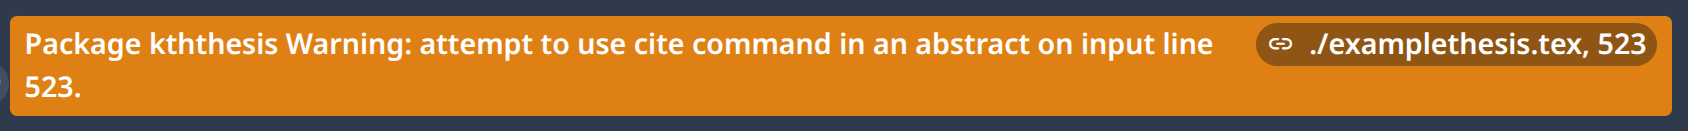
\includegraphics[width=0.99\textwidth]{README_notes/cite_warning_in_abstract.png}
  \end{center}
  \caption{Example of a warning for use of a citation in an abstract)}
  \label{fig:sec:cycle3CiteWarning}
\end{figure}

The combination of two red Exclamation Question Marks ({\NotoSansFont ⁉}, unicode U+2049) with the command between them (double underlined) was selected as: \first this string is unlikely in the user's text, \Second it was colored red to make it highly visible, and \third the offending command is double underlined to help make it visible (even to those who cannot see the color red). While this combination of characters is sometimes turned into an Interrobang glyph ({\NotoSansFont ‽}, unicode U+203D), I have chosen to use the Exclamation Question Mark glyph as I found the Interrobang too subtle visually. Additionally, when using struck-through or struck-out characters rather than the double underline, it was too hard to read the name of the command. While the PDF does not include the arguments to the \textbackslash cite or \textbackslash ref command - these are in the source \LaTeX\ .

\subsection{Tables and images in abstracts}
\label{sec:TablesAndImagesInAbstracts}
\warningExpl{This template and the tools that I have written to help enter the metadata into DiVA do \textbf{not} support tables and figures in abstracts.}

As an abstract in DiVA can contain HTML code, it is technically possible to make tables and include figures in a DiVA abstract. The problems are \first that I do not know a general means of transforming a table from LaTeX to HTML, and \Second I do not know of a good way of passing the image (or images) that might be in a LaTeX abstract (via tools) to DiVA. The second problem might be addressed by attaching the image files to the PDF and adding code to the generated HTML to refer to these images. One problem with this is that the images would probably need to be uploaded as supplemental/supporting material, and then there would need to be some tool to update the abstract to refer to this uploaded file.

In a recent correction that I suggested for a thesis abstract in DiVA, I manually created the table in HTML to match the table that was in the abstract in the printed thesis.
\warningExpl{The DiVA administrator who entered the thesis into DiVA had not put \emph{any} of the abstract in, but simply put "See file" in the abstract field!}

\subsection{Graphical or visual abstracts}
\label{sec:GraphicalAbstracts}

\gls{KI} has an excellent page about graphical abstracts, see \href{https://kib.ki.se/en/visualise-present/visualising-data/graphical-abstracts}{Graphical abstracts}. At present, this template does \textbf{not} provide any special support for graphical abstracts. One can use the usual mechanisms to include a figure in the abstract; however, see Appendix \ref{sec:TablesAndImagesInAbstracts}.

\warningExpl{I am unsure \first how to deal with such figures with respect to facilitating their inclusion in DiVA (Could it be uploaded separately as supplemental material?), and \Second it is unclear to me whether this graphical abstract would be placed before or after the keywords in the LaTeX file. This will require some further evaluation.}

\engExpl{Recently, I helped create such a graphical abstract (for a journal paper) using \texttt{tikz}. This might have some advantages in terms of accessibility if the \texttt{tikz} source code were available to a (screen) reader.}

\section{Cover illustration}
\label{sec:coverIllustration}
Some theses feature an optional cover illustration. Although I have not gotten an answer from the KTH communications unit about the specifications of the cover illustration, I have tried to infer something suitable from a DOCX file.
\warningExpl{Due to the lack of a specification for the cover illustration, one should treat this feature of my template as an experimental feature that will be subject to change. Use at your own risk.}

Two macros are introduced to make this process simpler, see \Cref{lst:SettingCoverIllustration}. The first (\texttt{\textbackslash coverIllustration}) provides the filename of the illustration to be used. The template includes an image1.png file. This blue rectangular image was taken from the DOCX template. The author should replace this file with the illustration that they want to use.

\textbf{NB} There are some constraints about what you can put on the cover. If in doubt, query KTH's \href{https://intra.kth.se/en/styrning/kths-organisation/verksamhetsstod/kommunikationsavdelningen-1.872391}{Communications Department (COM)}.

The second macro (\texttt{\textbackslash coverIllustrationCredit}) enables the author to acknowledge the creator of the illustration. Here, we will assume that the author has the creator's permission to include the illustration on the cover of their thesis. If the author has created their own illustration, then they do not need to specify any credit, as it is implicitly the work of the author.

\textbf{NB} The author may have to manually adjust the height and width options to the \texttt{\textbackslash includegraphics} command in the \texttt{kththesis.cls} file to get the results that they want. If you make the figure too large, it will appear on a second page and \textbf{not} on the cover. If this occurs, you need to reduce the height of the illustration.

\begin{lstlisting}[style=latexExampleForAuthors, caption={Configuring a cover illustration}, label=lst:SettingCoverIllustration]
% It is possible to have a cover illustration
\coverIllustration{figures/image1.png}
% if so, the author might acknowledge this or give the copyright information for it with:
\coverIllustrationCredit{A. B. Normal}
\end{lstlisting}

\section{While writing}
As was noted in \Cref{sec:authors}, the thesis template contains lots of examples, notes, and comments. One method to provide additional information is the use of \textbackslash todo. Several different types of \texttt{todo} notes have been used in the thesis. These are described in \Cref{sec:todonotes}.

\subsection{Conventions for todo notes}
\label{sec:todonotes}
The example thesis text includes extensive comments, directions, and warnings. These follow the form shown below:
\begin{lstlisting}
\generalExpl{Comments/directions/... in English}
\sweExpl{Text på svenska}
\engExpl{English descriptions about formatting}
\warningExpl{warning}  
\end{lstlisting}
and appear as:
\generalExpl{Comments/directions/... in English}
\sweExpl{Text på svenska}
\engExpl{English descriptions about formatting}
\warningExpl{warning}

Each of the above is a macro, so as usual in \LaTeX\ you can redefine it - even defining it to produce nothing! Several previous students have placed these re-definitions in the \fname{custom\_configuration.tex} file.

\subsection{Turning on and off the README\_notes}
As the various README notes are targeted at different readers, you may or not want to see them. It is very easy to turn them on or off by adding or removing a percent ('\%') character before the relevant \textbackslash begin\{comment\} and \textbackslash end\{comment\} comments around each set of notes.

For example, if you are a student writing a thesis, I suggest turning off everything except for the \fname{README\_author.tex} and \fname{README\_notes.tex} sets of notes. However, I would suggest keeping the other README files around (at least for a little while) as a source of examples of how to do things. Despite having spent a very large number of hours working on the template and drafts of students' theses, I find some of the README files very helpful as a reminder of how to do things.

\subsection{Removing the README\_notes}
At some point you will no longer want this README information. You can remove it by removing the line
\textbackslash include\{README\_notes/README\_notes\} -- from the \fname{examplethesis.tex} file. If you have removed the other README* files from the \dname{README\_notes} directory, you can then remove the \dname{README\_notes} directory.

\subsection{Removing the README\_notes}
At some point, you will no longer want this README information. You can remove it by removing the line
\textbackslash include\{README\_notes/README\_notes\} -- from the \fname{examplethesis.tex} file. If you have removed the other README* files from the \dname{README\_notes} directory, you can then remove the \dname{README\_notes} directory.

\subsection{Removing unused fonts}
This version of the template may also have some font information, in the form of Opentype Font files (with the extension ``.otf'') and TrueType Font font files (with the extension ``.ttf''). If you are not using these fonts (and no longer are using any of the README files), then you can delete these font files.

%\printglossary[type=readme,toctitle={Acronyms used in README notes}]


 % template instructions, not part of the thesis

\begin{comment}
% If you actually want to have the full table of National Subject Categories (temporarily) include this appendix
\subfile{README_notes/National_Subject_Categories}
\cleardoublepage
\end{comment}

\begin{comment}
% Information for examiners
\ifxeorlua
\cleardoublepage
%\documentclass[../examplethesis.tex]{subfiles}
%\begin{document}
\lstdefinestyle{PDF}{
language=[LaTeX]{TeX},
    breaklines=true,
    postbreak=\mbox{\textcolor{red}{$\hookrightarrow$}\space},
    basicstyle=\small\tt,
    keywordstyle=\color{blue}\sf,
    identifierstyle=\color{magenta},
    commentstyle=\color{cyan},
    backgroundcolor=\color{yellow!15},
    extendedchars=true,
    inputencoding=utf8,
    stringstyle=\ttfamily,
    morestring=[b]',
    tabsize=2,
    columns=flexible,
    morekeywords={Type, Action, JavaScript, obj, endobj, Length, Filter, FlateDecode, stream, endstream, JS, ASCIIHexDecode, startxref, xref, trailer, Size, Root, Catalog, OpenAction, AcroForm, Pages, Outlines, S,
    Kids, Count, Page, Parent, MediaBox, Contents, Resources, Font, ProcSet, PDF, Text, F1}
}

% Extend the XML style
\lstdefinestyle{myXML}{
    language=XML,
    columns=flexible,
    breaklines=true,
    showspaces=false,                       % Dont make spaces visible
    showtabs=false,                         % Dont make tabs visible
    breakatwhitespace=true,
    postbreak=\raisebox{0ex}[0ex][0ex]{\ensuremath{\color{red}\hookrightarrow\space}},
    basicstyle=\ttfamily\small,
    columns=fixed,
    escapechar = £,
    postbreak=\raisebox{0ex}[0ex][0ex]{\ensuremath{\color{red}\hookrightarrow\space}},
    morekeywords={dc:format, dc:title, dc:date, dc:type, dc:creator, dc:description, dc:subject, dc:source, dc:language, rdf:Alt, rdf:li, rdf:Bag, rdf:Seq, rdf:Description, rdf:Description, rdf:RDF, pdfaExtension:schemas, pdfaSchema:property, pdfaSchema:valueType, pdf:Producer, pdf:Keywords, pdf:PDFVersion, pdfaSchema:schema, pdfaSchema:prefix, pdfaSchema:namespaceURI, pdfaProperty:name, pdfaProperty:valueType, pdfaProperty:category, pdfaProperty:description,  xmp:CreateDate, xmp:ModifyDate, xmp:MetadataDate, xmp:CreatorTool, xmpMM:DocumentID, xmpMM:InstanceID, xmpMM:VersionID, xmpMM:RenditionClass, Iptc4xmpCore:CreatorContactInfo, Iptc4xmpCore:CiEmailWork, prism:complianceProfile, prism:pageCount, xmpTPg:NPages,  x:xmpmeta},
    %string=[bd]{|}      % Uncommenting this line eliminates the visible spaces in strings
% Support for Swedish, German and Portuguese umlauts
  literate=%
  {Ö}{{\"O}}1
  {Ä}{{\"A}}1
  {Å}{{\AA{}}}1
  {Ü}{{\"U}}1
  {ß}{{\ss}}1
  {ü}{{\"u}}1
  {ö}{{\"o}}1
  {ä}{{\"a}}1
  {å}{{\aa{}}}1
  {á}{{\'a}}1
  {ã}{{\~a}}1
  {é}{{\'e}}1
  {è}{{\`e}}1
  {€}{\euro}1%
  {’}{{\char13}}1
  {-}{{\textendash}}1
  {–}{{\textendash}}1
  {…}{{\ldots}}1
  {}{{BOM}{\;}{0xfeff}}{10},
}

\chapter{README and notes about the template for examiners}
\label{ch:readme_examiner}

This chapter, written by Gerald Q. Maguire Jr, describes the thesis template that I have developed for use at KTH Royal Institute of Technology (KTH) and provides some background about why it is the way that it is. This document provides some information for examiners (and possibly for administrators) about the template and especially how it can be used with some programs to help make the degree process easier for students, faculty, and administrators.

\textbf{This document is a work in progress and started from a DOCX document entitled ``Proposal for a standard thesis template''.}

An assumption for readers of this chapter is that you know KTH-speak, including the various acronyms used. I have spelled out some of the acronyms and given the Swedish for those that are of an administrative nature.

\section{Introduction for examiners}
\label{sec:IntroForExaminers}

Each year there are thousands of degree projects done by students at KTH Royal Institute of Technology. These are one of the core elements of undergraduate education, and producing high-quality degree projects is of interest to the faculty, students, administration, Universitetskanslersämbetet (UKÄ), and the public. The reasons for the work described in this document are \first I have been an examiner for a lot ($>$560) of degree projects and I want to help students by providing them a template to start with (avoiding the ``Blank paper'' barrier) and to help facilitate the degree project process, \Second the previous \LaTeX~template that used to be widely available to students at KTH was no longer being maintained, and \third the references from the KTH web to this template was removed by the Gemensamt verksamhetsstöd (GVS) Communications unit.

Since $\approx$2010, all KTH theses should have English and Swedish abstracts. Ideally, the thesis would also include keywords and titles in both English and Swedish. Moreover, this information is useful not only in the thesis itself but also in:
\begin{enumerate}
    \item The announcements of degree project presentations: As, in several programs, students doing degree projects need to be active listeners (really active participants) for some number of other degree project presentations; hence, it is desirable to announce these presentations and have students easily about to find this information and select which they would like to attend. Moreover, degree project presentations are supposed to be public, so it would be useful and foster their visibility if it was easy to make such announcements (in both English and Swedish).
    \item The final approved thesis needs to be entered into \foreignlanguage{swedish}{Digitala Vetenskapliga Arkivet (DiVA)} (both the metadata and the thesis itself) [There is a separate issue regarding whether the full-text is publicly available for not, but this is outside the scope of this document.]
    \item Reporting both English and Swedish titles in \foreignlanguage{swedish}{Lokalt adb–baserat dokumentationssystem (LADOK)}.
\end{enumerate}

Therefore, in my roles as an examiner, a (former) member of the “\foreignlanguage{swedish}{språkkommittén (referensgruppen för språkfrågor})” (until 31 March 2022), and to foster the production of theses in both English and Swedish, I have written a DOCX and \LaTeX~template for 1\textsuperscript{st} and second-cycle degree projects (as well as a \LaTeX~template for third cycle degree projects). Additionally, I have written some software to: \first make it easier to announce these events to make it easier for people to know about them so that they can attend, \Second make it easy to make the cover and apply it (or in the case of \LaTeX, integrate it into the template), and \third facilitate entering the metadata and thesis into DiVA. There is also an experimental effort to insert the two titles into LADOK (see \Cref{sec:JSONtoLADOK}).

The focus of this document will be on the \LaTeX\ template for 1\textsuperscript{st} and second-cycle degree projects. A separate document examines the DOCX version of the template, and a future document will examine the 3rd cycle \LaTeX~template. There is also a separate document that addresses the quality of the data in DiVA and LADOK, as the titles of theses as recorded in LADOK do not necessarily match those in either DiVA or the document itself (as a sample data point for the year 2020 and the School of Electrical Engineering and Computer Science (EECS), 9.4\% of the entries for titles in LADOK are in error). Additionally, since only a small number of students’ KTHIDs are recorded in the DiVA entry for their thesis, it is not easy to mechanically match the LADOK and DiVA records.
Most readers will only be interested in the high-level overview given in Sections~\ref{sec:AutomatingLaterSteps}, \ref{sec:accuracyAndEconomics}, \ref{sec:makeItSimpleFromTheStart}, and \ref{sec:AutomatingLaterSteps}. Some readers may be interested in accessibility, see \Cref{sec:accessibility}. The rest of the document should contain enough information to let someone else deal with the problems that remain. An easy to read user manual for the \LaTeX~template is integrated as an appendix in the template
\iflabelexists{ch:READMEnotes}{(see \Cref{ch:READMEnotes}).}
{- You have to include the \texttt{README\_notes/README\_notes.tex} file when compiling.}




\section{Accuracy and Economics}
\label{sec:accuracyAndEconomics}

An earlier first-cycle thesis  looked at the automation of entering a thesis and its metadata into DiVA and found that a large fraction of existing entries with manually entered metadata in DiVA had errors in them and also estimated that the total number of full-time equivalent (FTE) hours spent entering this data was several FTEs equivalent. Note that the change to having only administrative staff enter the metadata has not eliminated the problem of errors in data entry.
\begin{description}[labelwidth =\widthof{\textbf{Hypothesis}}, leftmargin = !]
\item[Hypothesis] Incorporating the relevant data into the thesis document will facilitate both announcements and DiVA data entry.

\item[Approach] Make this data readily available via the template and collect \& output it in a 
“For DIVA” set of information at the end of the Portable Document Format (PDF) document. Additionally, try to minimize the need to manually enter information by taking information from the Canvas course room.
\end{description}

Given the hypothesis stated above, the overall flow is shown in \Cref{fig:LogicalOverviewOfWhatIsDone}. 
\tikzset{
    processBox/.style={rectangle, rounded corners, minimum width=3cm, minimum height=1cm,text centered, font=\sffamily, draw=black, fill=red!20},
    destinationBox/.style={rectangle, rounded corners, minimum width=3cm, minimum height=1cm,text centered, draw=black, fill=green!10},
    arrow/.style={thick,->,>=stealth}
}

\begin{figure}[!ht]
\resizebox{\textwidth}{!}{%
\begin{tikzpicture}
[align=left,node distance=2cm]


\node (latexFile) [tape,tape bend top=none,draw,font=\sffamily] {\LaTeX file};
\node (PDFfile) [tape,tape bend top=none,draw,font=\sffamily, above of=latexFile] {PDF file};
\node (DOCXFile) [tape,tape bend top=none,draw,font=\sffamily, below of=latexFile] {DOCX file};

\node (extractor) [processBox, right=1cm of latexFile] {Extractor};
\node (jsonFile) [tape,tape bend top=none,draw,font=\sffamily, right=0.5cm of extractor] {JSON file};
\node (start) [processBox, right=0.5cm of jsonFile] {JSON\_to\_calendar};

\node (jsontoMODS) [processBox, below of=start] {JSON\_to\_MODS};
\node (modsFile) [tape,tape bend top=none,draw,font=\sffamily, below of=jsontoMODS] {MODS file};
\node (diva) [destinationBox, right=1cm of modsFile] {Import into DiVA};

\node (calendarEvent) [destinationBox, right=1cm of start] {Canvas calendar event};
\node (announcement) [destinationBox,  above of =calendarEvent] {Canvas announcement};
\node (cortinaCalendarEvent) [destinationBox,  right=0.5cm of start, below of=calendarEvent] {KTH Cortina calendar event};
\draw [arrow] (latexFile) --  (extractor.west);
\draw [arrow] (PDFfile) --  (extractor.west);
\draw [arrow] (DOCXFile) --  (extractor.west);
\draw [arrow] (extractor) --  (jsonFile.west);
\draw [arrow] (jsonFile) --  (start.west);
\draw [arrow] (start.east) --  (announcement.west);
\draw [arrow] (start.east) -- (calendarEvent);
\draw [arrow] (start.east) -- (cortinaCalendarEvent.west);
\draw [arrow] (jsonFile) --  (jsontoMODS.west);
\draw [arrow] (jsontoMODS) --  (modsFile);
\draw [arrow] (modsFile) --  (diva);
\end{tikzpicture}
}
\caption{From PDF file, \LaTeX\;project, or DOCX file generate announcement, calendar entries, and a MODS file for import into DiVA}
  \label{fig:LogicalOverviewOfWhatIsDone}
\end{figure}
\FloatBarrier

\section{Make it simple from the start}
\label{sec:makeItSimpleFromTheStart}

\Needspace*{3\baselineskip}
The key to the process shown in \Cref{fig:LogicalOverviewOfWhatIsDone} is collecting all of the necessary data in the thesis and organizing all of the data so that it is easy to extract (hence the limitation to my templates). It is this information and its organization that makes the magic ``Extractor'' possible.

If a Canvas course room is set up for degree projects, one can greatly simplify the many processes involved for all the stakeholders (students, faculty, and staff). The Canvas course\_id is the number following the string ``https://canvas.kth.se/courses/''.

The student (or student) doing a degree project is/are assumed to be enrolled in the Canvas course room and that one knows the student’s e-mail address (or in the case of a first-cycle thesis, possibly two students’ addresses), and the e-mail address of the examiner and the supervisor(s). Multiple supervisors are supported, both internal to KTH and external to KTH.

For two first-cycle students (with e-mail addresses s1@kth.se and s2@kth.se), myself as the examiner (maguire@kth.se), and Anders Västberg (vastberg@kth.se) as the academic supervisor and an unknown supervisor at a company – together with the program code and course code, generating s pre-configuring of the \LaTeX~template is as simple as two (single line) commands, shown in \Cref{lst:createCustomizeJSON} and \Cref{lst:customizeLaTeXproject}. The first command (shown in \Cref{lst:createCustomizeJSON}) gets relevant data from Canvas and makes a JSON file (by default named \texttt{customize.json}) with the relevant information in it. The \texttt{xxx} in the command will generate dummy entries for an external supervisor.

\Needspace*{7\baselineskip}
\begin{lstlisting}[language={bash}, caption={Example of creating a customized JSON file for two students}, label=lst:createCustomizeJSON]
./create_customized_JSON_file.py --canvas_course_id 31167 --author s1@kth.se --author2 s2@kth.se --language eng --programCode TIDAB --Examiner maguire --Supervisor vastberg   --Supervisor2 xxx --courseCode II142X  --exam högskoleingenjör
\end{lstlisting}

\Needspace*{14\baselineskip}
The second command (shown in \Cref{lst:customizeLaTeXproject}) takes a local zip file of the \LaTeX\;project (in \texttt{z23.zip}) and adds the customization information to it. The ``--initialize'' option indicates that the program should replace any of the project's existing customization information concerning the author(s), examiner, and supervisor(s). The program produces a \texttt{z23-modified.zip} file - that I rename based on the student's name and then send to the student. The student only has to upload this file into Overleaf, and off they go! If they then invite the examiner and supervisor(s) to the Overleaf project, these people can directly see what the student is doing, comment, etc. I generally suggest that the student rename their Overleaf project to put their name into the project name; thus, I can search the Overleaf projects easily to find the project of this student or students. Creating a customized \LaTeX\;project for each student greatly simplifies things and collects some of the needed data already at the start of the degree project.

\Needspace*{4\baselineskip}
\begin{lstlisting}[language={bash}, caption={Create a customized \LaTeX\;project}, label=lst:customizeLaTeXproject]
./customize_LaTeX_project.py --json customize.json --file z23.zip --initialize
\end{lstlisting}

\Needspace*{7\baselineskip}
For a second-cycle thesis, an example of the first command is shown in \Cref{lst:createCustomizeJSONmasters}. The same second command is used to make the customized \LaTeX\;project for the second-cycle student.
\begin{lstlisting}[language={bash}, caption={Create a customized \LaTeX\;project for a Master's student}, label=lst:createCustomizeJSONmasters]
./create_customized_JSON_file.py --canvas_course_id 33514 --author s1 --language eng --programCode TCSCM  --Examiner maguire --Supervisor vastberg   --Supervisor2 xxx  --courseCode DA231X  --exam master
\end{lstlisting}

\Cref{tab:examValues} shows the types of degrees supported as the value for the ``--exam'' option. Note that the values are in Swedish, an acronym, `both', or `both\_same'. The case of `both\_same' is for the case when both when the field of technology and main subject is the same, \ie \foreignlanguage{swedish}{både om dessa områden har samma benämning}. In most cases, the value should be known, but it may be necessary to ask the student what degree they will apply for. This information is necessary because it makes a difference in the KTH cover and is also needed for the DiVA entry.

\begin{table}[!ht]
    \caption{Supported exam values}
    \label{tab:examValues}
    \begin{tabular}{L{3cm}|L{4.5cm}|L{4.5cm}}
      \textbf{value} & \textbf{English name} & \textbf{Svenskt namn}\\
      \hline
kandidat & Degree of Bachelor of Science & Kandidatexamen\\
högskoleingenjör & Degree of Bachelor of Science in Engineering & Högskoleingenjörsexamen\\
civilingenjör & Degree of Master of Science in Engineering & Civilingenjörsexamen\\
magister & Magister & Magisterexamen\\
master & Degree of Master of Science & Masterexamen\\
arkitekt & Degree of Master of Architecture & Arkitektexamen\\
ämneslärar & Degree of Master of Science in Secondary Education & Ämneslärarexamen\\
CLGYM & Master of Science in Engineering and in Education & Civilingenjör och lärare\\
KPU & KPU (supplementary teacher education) & KPU (kompletterande pedagogisk utbildning)\\
both & Both Degree of Master of Science in Engineering and Degree of Master of Science &
        Både civilingenjörsexamen och masterexamen\\
both\_same & Both Degree of Master of Science in Engineering and Degree of Master of Science & Både civilingenjörsexamen och masterexamen\\
\hline
   \end{tabular}
\end{table}
\FloatBarrier


\subsection{Using Information from Canvas and putting information into Canvas}
In order to minimize the amount of data that needs to be manually entered it is important to ask several questions:
\begin{itemize}
    \item What kind of information can be gotten from Canvas?
    \item What can you do with this data?
    \item What information can be put into Canvas?
\end{itemize}

Given the course course\_id (31167 and 33514 in the examples above), you can look up information about the student via the Canvas course room. For example, if we assume the course\_id is 33514 (the EECS second-cycle degree project Canvas course room for lots of different courses) and the student is taking the course DA231X. When the student is enrolled in this Canvas course room they are added to a section that has their course code in it. For example:
\begin{quote}
    Section for the course DA231X VT22-2 Degree Project in Computer Science and Engineering, Second Cycle
\end{quote}

Canvas sections are a very powerful mechanism for organizing students. A student can be in up 18 different sections in a given Canvas course room. For example, it is possible to create sections for each of the examiners (assumed to be Examiners in the Canvas course room) and the academic supervisors (assumed to be Teachers in the Canvas course room). Now one can add the student to the examiner section and supervisor(s) section(s). The result is that the student now appears in these different sections, see \Cref{fig:studentInMultipleSections}. The information about what sections each student is in can be seen via the ``People'' course navigation button - in the ``Section'' column.

\begin{figure}[!ht]
  \begin{center}
    \small
    \begin{tabular}{p{9cm} p{2cm}} 
    XXXXX, XXXXXXX & Student \\
    ExaminersLastname, ExaminersFirstname & Student \\
    Section for the course DA231X VT22-2 Degree Project in Computer Science and Engineering, Second Cycle & Student \\
 \end{tabular}
  \end{center}
  \caption{A student in multiple sections – one for the course, one for the supervisor, and one for the examiner. The supervisor's name has been anonymized.)}
  \label{fig:studentInMultipleSections}
\end{figure}

This greatly simplifies the work for the examiner and supervisor as now they can choose to view the gradebook and only need to see their students, as shown in \Cref{fig:examinersViewOfGradebook}.
 	
\begin{figure}[!ht]
  \begin{center}
    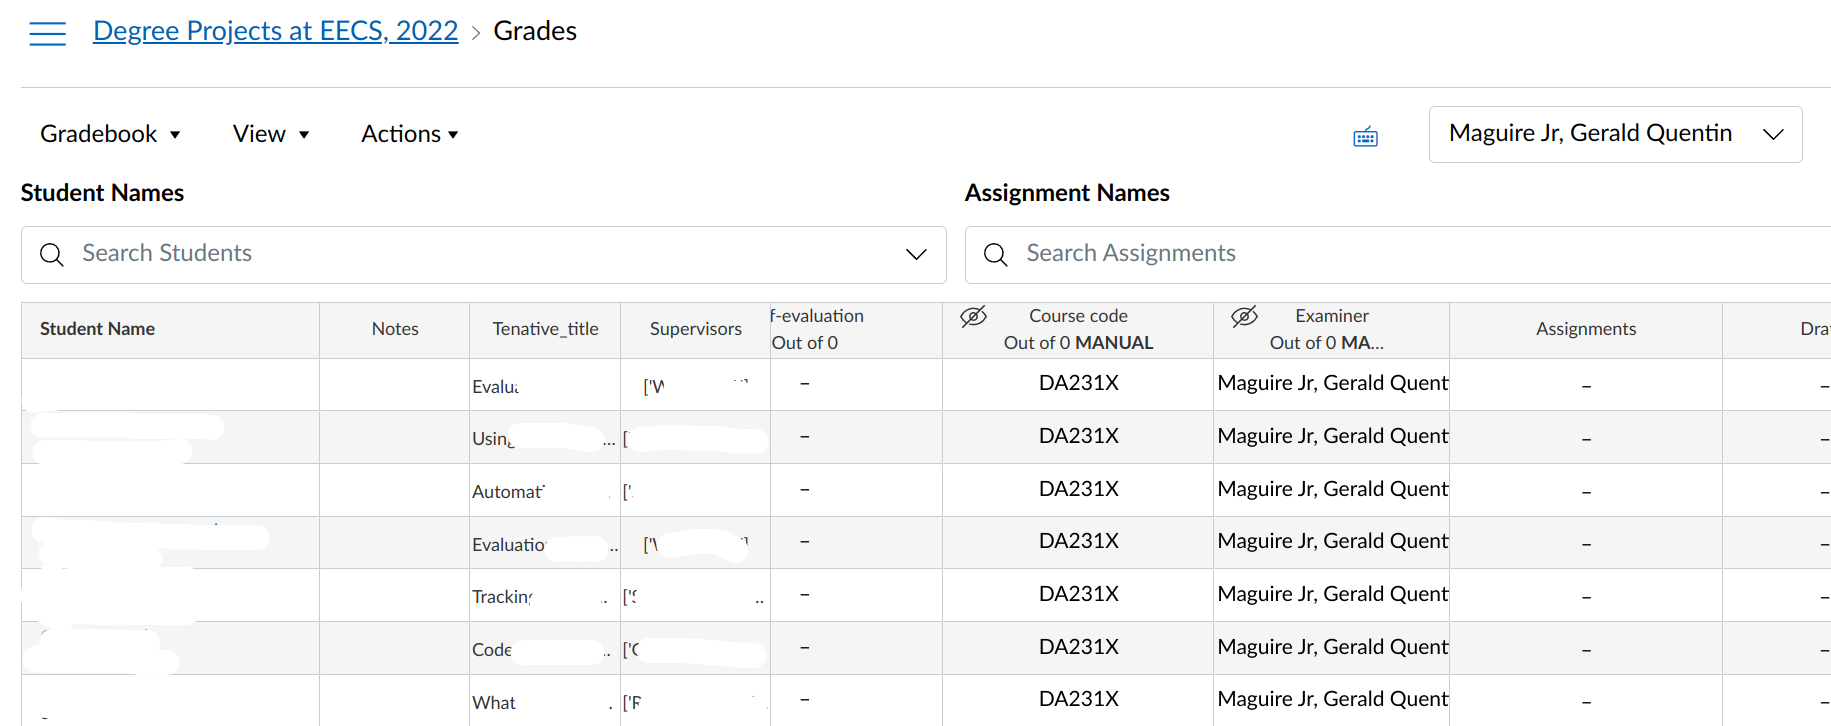
\includegraphics[width=0.99\textwidth]{README_notes/README-examiner-figures/part-of-my-students-Screenshot_20220325_152422-edited.png}
  \end{center}
  \caption{Examiner's view of the gradebook)}
  \label{fig:examinersViewOfGradebook}
\end{figure}

Note that in \Cref{fig:examinersViewOfGradebook}, there are two columns “Course code” and “Examiner”. These are what I call \textit{administrative assignments} and the students do not need to see them (hence the eye symbol with a slash through it – indicating these are hidden from the students). In the “Course code” assignment, I have given the student a “grade” that is the course code of their degree project. This way it is very easy to see what course code a student is enrolled in – as an examiner or supervisor may have students enrolled in several different course codes. This “grading standard”\footnote{What Canvas calls a grading standard is often called a grading scale.} was created from the list of all the EECS second-cycle course codes that share this same Canvas course room. The “Examiner” column contains a “grade” that is the name of the examiner assigned for this student. The examiner “grading standard” is created from the list of all of the examiners in the Canvas course room. In the same way that a teacher can assign a grade, if you click on the gradebook cell for a student, you get a pull-down list of all of the possible “grades” in this case the list of examiners, see \Cref{fig:listOfExaminers}.
\begin{figure}[!ht]
  \begin{center}
    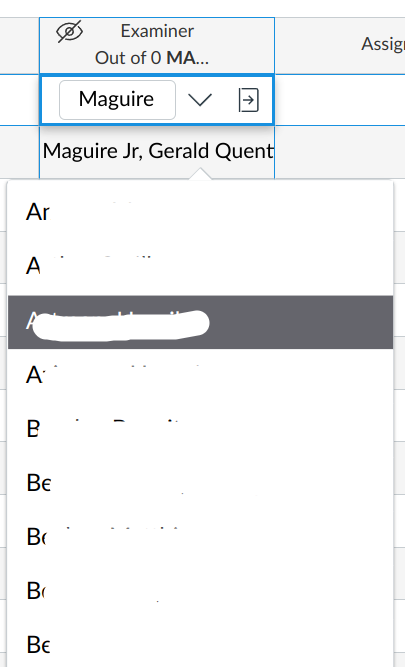
\includegraphics[width=0.5\textwidth]{README_notes/README-examiner-figures/top-of-the-list-of-examiners-Screenshot_20220325_153634.png}
  \end{center}
  \caption[List of examiners]{List of examiners (with the names erased to avoid GDPR problems)}
  \label{fig:listOfExaminers}
\end{figure}

Did I have to manually enter all of the course codes for the 687 students in the course room? No, I used a script via the command shown in \Cref{lst:addCourseCodesForStudentsInCourse}.  This required that initially the grading standard with course codes be created. It was created with the command shown in \Cref{lst:insertCourseCodeGradingStandard}.
\Needspace*{3\baselineskip}
\begin{lstlisting}[language={bash}, caption={add\_course\_codes\_for\_students\_in\_course.py}, label=lst:addCourseCodesForStudentsInCourse]
./add_course_codes_for_students_in_course.py 33514
\end{lstlisting}
\Needspace*{3\baselineskip}
\begin{lstlisting}[language={bash}, caption={insert\_course\_code\_grading\_standard.py}, label=lst:insertCourseCodeGradingStandard]
./insert_course_code_grading_standard.py 33514
\end{lstlisting}
\Needspace*{3\baselineskip}
The grading standard for examiners (and even one for teachers as supervisors) is created with the command shown in  \Cref{lst:insertTeachersGradingStandard}. To create the teachers grading standard you leave off the ``--emaniners'' option.

%% the following conditional is needed to avoid problems with "--" in the listing when using pdflatex
\ifxeorlua
\begin{lstlisting}[language={bash}, caption={insert\_teachers\_grading\_standard.py}, label=lst:insertTeachersGradingStandard]
./insert_teachers_grading_standard.py –-examiners 33514
\end{lstlisting}
\else
\begin{lstlisting}[%language={bash}, 
  basicstyle=\ttfamily, extendedchars=false,
caption={insert\_teachers\_grading\_standard.py}, label=lst:insertTeachersGradingStandard]
./insert_teachers_grading_standard.py –-examiners 33514
\end{lstlisting}
\fi

The command line shown in \Cref{lst:insertTeachersGradingStandard} creates a grading standard with the suffix “\_Examiners”. Note that all of these grading standards are \textit{course specific} grading standards, so they are invisible outside of this course room. One caution about the use of grading standards is that if the list of course codes or list of teachers/examiners changes – there can be problems with the mappings as the grading standard creates a mapping between a numeric grade and a string (the course code or name); therefore, they should only be generated once at the start of the course when the full list of values is known.

So clearly we can have information about the student, supervisors (who are teachers in the course), and examiner in the Canvas course room. Then since these people are in the Canvas course room we can know their sort-able name, KTHID, e-mail address, etc. Clearly, the students were added to the course when they were enrolled in the course. How did the teachers and examiners get into the course? These people were added to the course by a script that IT runs that takes this data from Kurs- och programplaneringssystemet (KOPPS)!

\subsection{How can we associate students with examiners and supervisors?}
In the case of the computer science (CS) students, the exjobb coordinator XXXXX\footnote{The person's name has been removed, to avoid issues with GDPR.} has a spreadsheet with the student’s name, working title, examiner, and supervisors in it. It has a sheet named “Closed” that contains information about the students who have been assigned an examiner and supervisor. \Cref{fig:spreadsheetOfCSStudents} shows the column headings of the spreadsheet “Masters\_thesis\_proposals-CS-P3-2022a.xlx” (this is my local file name for the spreadsheet).
	
\begin{figure}[!ht]
  \begin{center}
    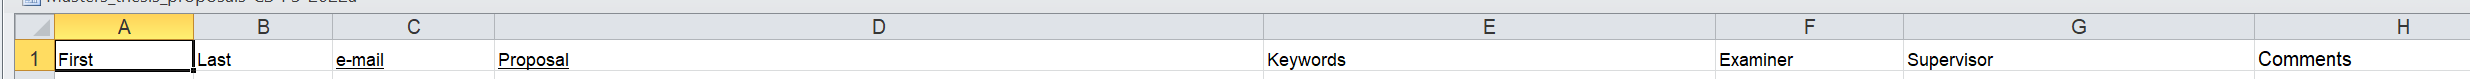
\includegraphics[width=0.99\textwidth]{README_notes/README-examiner-figures/sheet-columns-Screenshot_20220325_155622.png}
  \end{center}
  \caption{Columns in the `Closed' sheet of spreadsheet of CS students)}
  \label{fig:spreadsheetOfCSStudents}
\end{figure}

\Needspace*{6\baselineskip}
A script takes the data from this spreadsheet and adds the information to the Canvas gradebook with the command shown in \Cref{lst:insertExaminersAndSupervisorsFromSpreadsheet}.
\begin{lstlisting}[language={bash}, caption={insert-examiners-and-supervisors-from-spreadsheet.py}, label=lst:insertExaminersAndSupervisorsFromSpreadsheet]
./insert-examiners-and-supervisors-from-spreadsheet.py  33514   "Masters_thesis_proposals-CS-P3-2022a.xlsx"  
\end{lstlisting}
The script uses the student’s e-mail address to look up the student in the Canvas course room, then adds the student to the examiner’s section and updates the “Examiner” grade for this student to show this assigned examiner. It also adds the contents of “Proposal” field from the spreadsheet as text in a custom column in the gradebook called “Tentative\_title” and adds the list of supervisors to the custom column called “Supervisors” – see \Cref{fig:examinersViewOfGradebook}. Note that this program uses a JavaScript Object Notation (JSON) file, \texttt{spreadsheet\_aliases-33514.json}, containing aliases for each of the examiners and supervisors. \Cref{lst:aliasFile} shows part of the alias file.
\Needspace*{15\baselineskip}	
\begin{lstlisting}[language={Python}, caption={Some of the contents of an alias file for a course}, label=lst:aliasFile]
{
    "examiners": {
        "Anders Västberg": "Västberg, Anders",

        "Gerald Maguire": "Maguire Jr, Gerald Quentin",
        "Gerald  Q.  Maguire": "Maguire Jr, Gerald Quentin",

    },
    "teachers": {
    
    }
}
\end{lstlisting}

The alias file takes the names used in the spreadsheet (the name shown on the left in the listing above) and maps them to the sortable names used in Canvas (the name shown on the right in the listing above). While this adds a little more complexity, it addressed the problem that the names used in the spreadsheet are not always consistent or even complete.

The availability of information in Canvas also suggests that some of the arguments that were shown earlier for the script \texttt{create\_customized\_JSON\_file.py} are actually unnecessary and the program can figure them out given the course\_id and student’s e-mail address. However, some things are not accessible directly from Canvas, for example, I have not been able to figure out what exam a student intends to apply for following their degree project course. Another example of missing information is the program code; however, this information is in LADOK and Canvas has the LADOK identifier for each student; however, my script to access LADOK is currently not working.
\Needspace*{8\baselineskip}
\subsection[What happens if I do not have such a spreadsheet?]{What happens if I do not have such\\ a spreadsheet?}

A Canvas administrator can add students to the examiner’s and supervisor’s sections, as shown in \Cref{fig:sectionEntrollments}. Note that the input field can do partial matches on the text that you enter and will give you a list of the partially matching entries and then you can click on one and then click on Update. 
 	
\begin{figure}[!ht]
  \begin{center}
    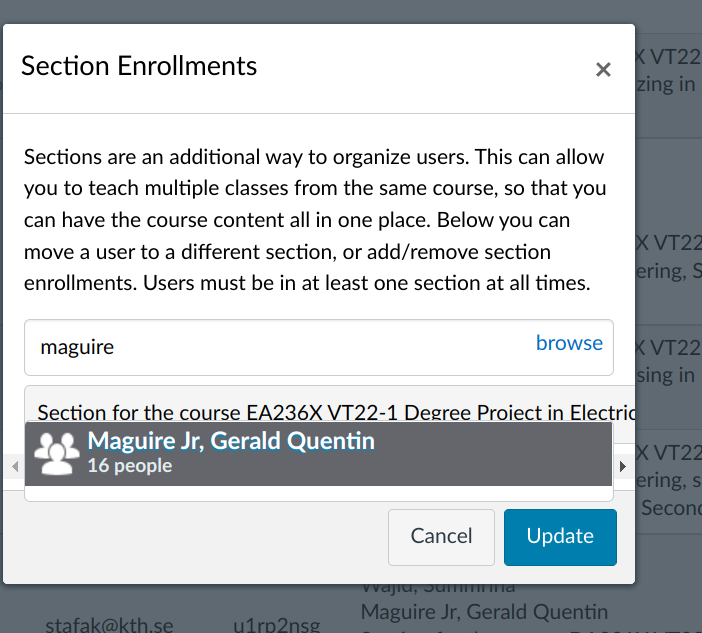
\includegraphics[width=0.99\textwidth]{README_notes/README-examiner-figures/edit-sections-Screenshot_20220325_161529.png}
  \end{center}
  \caption{Section enrollments)}
  \label{fig:sectionEntrollments}
\end{figure}
\FloatBarrier

To get the Section Enrollments editing box popup (shown above) – you go to the “People” page – find the student (either scrolling down the page or starting to type the student’s name in “Search people” box (shown in \Cref{fig:peopleSearchbox}) then click on the vertical three dots on the right side of the row for this student and click on Edit section (as shown in \cref{fig:editSectionsButton}).
\begin{figure}[!ht]
  \begin{center}
    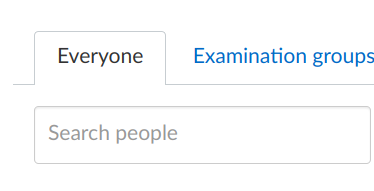
\includegraphics[width=0.5\textwidth]{README_notes/README-examiner-figures/Search-people-Screenshot_20220325_161811.png}
  \end{center}
  \caption{Search people box on People page}
  \label{fig:peopleSearchbox}
\end{figure}
	
\begin{figure}[!ht]
  \begin{center}
    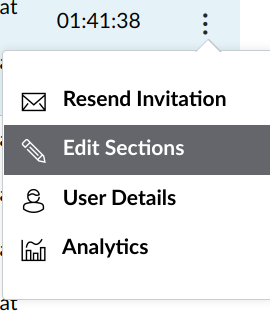
\includegraphics[width=0.5\textwidth]{README_notes/README-examiner-figures/edit-section-cmd-Screenshot_20220325_162252.png}
  \end{center}
  \caption{Three vertical dots and Edit Sections button}
  \label{fig:editSectionsButton}
\end{figure}
\FloatBarrier

Now that we have tied together the student, examiner, and supervisors; we can make use of that information in many ways. One of these ways was to create the customized \LaTeX\;project described earlier. The next section will explain some of the additional steps in the degree project that can be partially automated.
\Needspace*{12\baselineskip}
\section{Automating later steps in the degree project}
\label{sec:AutomatingLaterSteps}
There are many different steps in the degree project that can be facilitated by using the information from the Canvas course room and from the student's thesis. An example of one of these is making an announcement for the student's oral presentation (described in \Cref{sec:makingAnAnnouncement}). Another example is facilitating entering the metadata about the thesis into DiVA (see \Cref{sec:facilitatingDiVAentry}).

\subsection{Making an announcement}
\label{sec:makingAnAnnouncement}
When the examiner has set a time, place, \ldots for the student's oral presentation, then assuming that a student has submitted their thesis with the information in the “For DIVA” pages and that this information includes the information about the opponent(s) and presentation (\eg time, place, zoom link), the steps to make an announcement are:
\begin{enumerate}
    \item Save the PDF file of the thesis, for example \texttt{oscar.pdf}
    \item Extract the “For DIVA” information as JSON, as shown in \Cref{lst:extractPseudoJSONFromPDFforOscarFileToJSON}\footnote{For information about an alternative way to get the JSON file, see \Cref{sec:optimizeJSONToMods}.}
    
    If acronyms are used in the abstracts, you can add the “--acronyms acronyms.tex” argument to the extract command line and the program will process the acronyms from the acronyms.tex file (this means that you will also need this file). The output of the program is a JSON file (oscar.json) that can subsequently be used to make an announcement.
    
    \item Make the announcement for a Canvas course room (in this case, for a Canvas course room with course\_id 11), as shown in \Cref{lst:jsonToCalenarforOscar1}.
    
    Replace 11 with the course\_id of the Canvas course room, for example, 33514 for the EECS second-cycle degree projects during 2022.
\end{enumerate}
\Needspace*{7\baselineskip}
\begin{lstlisting}[language={bash}, caption={extract\_pseudo\_JSON-from\_PDF.py for Oscar}, label=lst:extractPseudoJSONFromPDFforOscarFileToJSON]    
   ./extract_pseudo_JSON-from_PDF.py --pdf oscar.pdf --json oscar.json
\end{lstlisting}

\begin{lstlisting}[language={bash}, caption={JSON\_to\_calendar.py for Oscar}, label=lst:jsonToCalenarforOscar1] 
./JSON_to_calendar.py -c 11 --json oscar.json
\end{lstlisting}
The command line shown in \Cref{lst:jsonToCalenarforOscar1} will publish the announcement in \first Canvas course 11, \Second in the Canvas course’s calendar, and \third (eventually) in the KTH Calendar. To publish a KTH calendar event, the software supports the development version of the KTH Cortina API. However, this is API not yet in production and requires a KTH Cortina Access Key.

 For more information see Sections~\ref{sec:whatCanweDoWithTheJSONfile} and \ref{sec:otherVariantsofJSONtoCalendar}.

\subsection{Making a cover and applying it}
\label{sec:makingACover}
As of December 2021, there is a new cover for 1\textsuperscript{st} and second-cycle theses at KTH. Information about this is at \url{https://intra.kth.se/en/administration/kommunikation/mallar/avhandlingarochexamensarbeten/skapa-ett-omslag-till-ditt-exjobb-1.479838}.

When the student is writing their thesis, they can set up the title and subtitle in English and Swedish by simply editing the relevant lines in the \LaTeX~file, see \Cref{lst:titleSubtitleEtc}. This is further described in detail in \Cref{sec:putInformationIntoLatexTemplate}  
\iflabelexists{ch:READMEnotes}{and \Cref{ch:READMEnotes}}
{- You have to include the \texttt{README\_notes/README\_notes.tex} file when compiling to get additional information.}

\Needspace*{12\baselineskip}
\begin{lstlisting}[language={[LaTeX]TeX}, caption={Title and subtitle in the two languages}, label=lst:titleSubtitleEtc] 
\title{This is the title in the language of the thesis}
\subtitle{A subtitle in the language of the thesis}

% give the alternative title - i.e., if the thesis is in English, then give a Swedish title
\alttitle{Detta är den svenska översättningen av titeln}
\altsubtitle{Detta är den svenska översättningen av undertiteln}
% alternative, if the thesis is in Swedish, then give an English title
%\alttitle{This is the English translation of the title}
%\altsubtitle{This is the English translation of the subtitle}
  \end{verbatim}
  \caption{Title, subtitle, etc.)}
  \label{fig:titleSubtitleEtc}
\end{lstlisting}

In the case of the \LaTeX\;project, the cover is automatically made and updated as the student writes their thesis. The only things that are needed for the cover that are missing is the exam that the student is going to take out and the TRITA number. We will assume that the student has entered the exam that they are going to apply for in their \LaTeX~file.

Within School of XXX\footnote{Name replaced to neutralize the template.}, the Office of Student Affairs assigns the TRITA number when the examiner has approved the thesis and submitted the PDF file of the approved thesis\footnote{This PDF file is supposed to have the front and back covers; however, as can be seen from the temporal ordering there is a problem as the back cover is made and applied \textbf{before} the number is assigned. One possible solution for this would be to not apply the back cover, but rather have the back cover created and applied by the Office of Student Affairs after they have assigned the TRITA number. Another possible solution would be to tell the examiner the TRITA number so that it can be added to the project and the cover and MODS file made. I think that ideally the TRITA number should be assigned by a program (and stored in a database) and the same program can make and add to the PDF of the thesis. Additionally, the assignments of TRITA numbers in the database can be sent to the archiving unit each year.}. The TRITA number needs to be \first added to the project before generating the final PDF file or \Second alternatively it can be entered by editing the placeholder text on the back cover when the TRITA number is assigned. Note that in the latter case, this data has to be (a) added to the JSON file used to make the MODS file (see \Cref{sec:facilitatingDiVAentry}) or (b) manually edited in DiVA entry.

So what we have seen (in this and other sections) is that we can use the information from Canvas and the thesis itself for simplifying many steps of the degree project process. For example, by having the thesis itself have both the English and Swedish titles and subtitles, it should be easier to add this information to both DiVA and LADOK. The underlying assumption is that the correct and relevant data will be in the Canvas course room and in the thesis itself!
\clearpage

\subsection{To facilitate entering a thesis into DiVA – make a MODS file}
\label{sec:facilitatingDiVAentry}
Assuming that a student has submitted a thesis with the information in the “For DIVA pages” that includes the information for the DIVA entry and the examiner has approved the thesis.

The same steps as described in \Cref{sec:makingACover} are made to save the PDF file and extract the “For DIVA” information as JSON\footnote{For information about an alternative way to get the JSON file, see \Cref{sec:optimizeJSONToMods}.}. This JSON file is then used to make a MODS file via the command shown in \Cref{lst:jsonToMODSforOscar}. Note that in this case, we assume that the person running the program knows the TRITA number; otherwise, the value of the TRITA number in the JSON file is used.
\Needspace*{4\baselineskip}
\begin{lstlisting}[language={bash}, caption={JSON\_to\_MODS.py for Oscar}, label=lst:jsonToMODSforOscar] 
./JSON\_to\_MODS.py -c 11   --json oscar.json --trita "TRITA-XXX-EX-2021:xxxx"
\end{lstlisting}

One way of getting the JSON information to make the MODS file is given in \Cref{sec:optimizeJSONToMods}. A description of how the JSON is converted to a MODS file is given in \Cref{sec:JSONtoMODSfile}.

\section{Can someone else use these programs?}
The source code is at \url{https://github.com/gqmaguirejr/E-learning}. Get the programs from the github, then create a config.json file to provide your Canvas access token and the URL of the Canvas instance you want to use, for details see \url{https://canvas.kth.se/courses/11/pages/making-a-config-dot-json-file-to-make-life-simpler} 

To run the program to make announcements and calendar entries for a course room requires the program and appropriate permissions  to post announcements in a course and insert course calendar events (for example, if the user is a Teacher in the specific Canvas course room or as a Canvas administrator). To make the entry in the KTH Calendar requires a KTH Cortina access key. Making the MODS file does not require any specific permissions as the program is run locally.

To change sections (adding/removing/\ldots a user to/from a section) requires the permissions of a Canvas administrator. However, this is something that E-learning should change about the KTH Canvas configuration; as this should be something that the examiner(s) or course-responsible persons should be able to do. Additionally, the KTH Cortina Calendar API requires an access key (which you have to get from the IT unit).

\Needspace*{12\baselineskip}
\section{\LaTeX~template in Overleaf}
A \LaTeX~template in Overleaf is at \url{https://www.overleaf.com/read/qxvttmmqbgdt} - this is the version used by many students.

Details about using the template are in  
\iflabelexists{ch:READMEnotes}{\Cref{ch:READMEnotes}.}
{xxxx - You have to include the \texttt{README\_notes/README\_notes.tex} file when compiling to get additional information.}
Note that the rest of this document goes into deep detail about \textit{how} the \textbf{template} works and \textit{how} the \textbf{programs} work. The primary intention is to give the information necessary so that someone else can take over the template and programs. Also note that \Cref{sec:accessibility} addresses issues about accessibility.
 
\section{Put information into \LaTeX~template to generate a draft or final thesis}
\label{sec:putInformationIntoLatexTemplate}

\Cref{fig:sampleTitlePage} shows the title page of a fictitious thesis created using a \LaTeX~template that I have developed. The idea is to capture in the thesis itself all of the information needed for this title page, the cover pages, the announcement of the oral presentation, and for reporting the final approved thesis in DiVA via the thesis itself.

\begin{figure}[!ht]
  \begin{center}
    \fbox{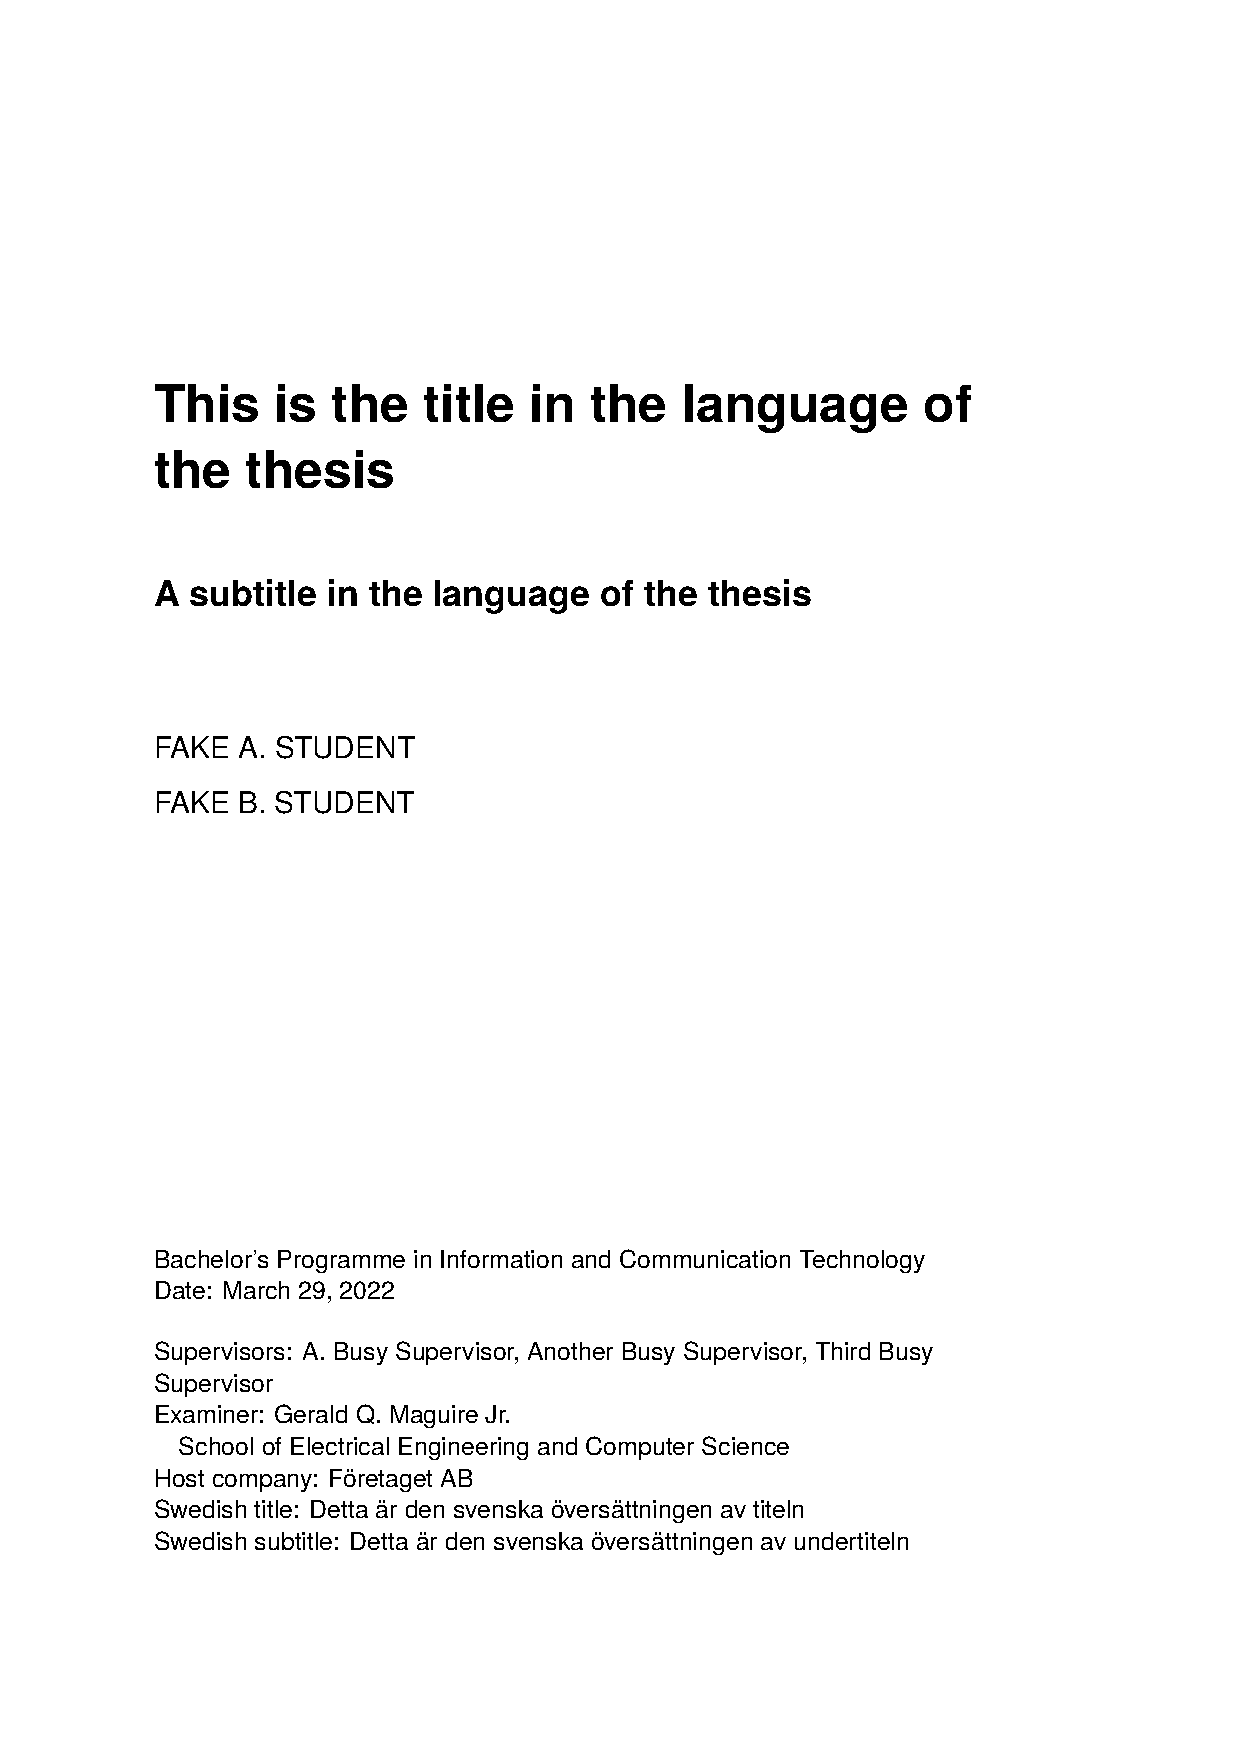
\includegraphics[width=0.85\textwidth]{README_notes/README-examiner-figures/Title-page-20220329.pdf}}
  \end{center}
  \caption{Example of a title page}
  \label{fig:sampleTitlePage}
\end{figure}
\clearpage

For the current documentation of the template for these details, please see the file “README\_notes.tex” in the template itself - 
\iflabelexists{ch:READMEnotes}{\Cref{ch:READMEnotes}.}
{You have to include the \texttt{README\_notes/README\_notes.tex} file when compiling to get additional information.}
What follows includes some older examples – so there may be differences in the details between these examples and the current template.

For the purpose of this document, the following information is present in the order of this exposition, not necessarily the order it is in the \LaTeX~source file. However, all of this information is prior to \textbackslash begin{document}. In particular, information that should be knowable at the start of the degree project is placed into a file named \texttt{custom\_configuration.tex} – to make it easier to pre-configure a project for a student or students (as was described in \Cref{sec:makeItSimpleFromTheStart}).

Information about the title and the student author(s) of the thesis is entered via the set of commands as shown in Listings~\ref{lst:titles} and \ref{lst:authors}. Note that you can have either one or two authors (the latter should generally only occur in the case of a first-cycle degree project). There are several other elements of metadata collected about the student (primarily driven by the current author metadata fields in DiVA). A brief description of them and why they are there are given below:
\begin{itemize}
    \item One might question why have an e-mail address (when under the current policy is that the student will lose their e-mail address upon graduation)? One of the main reasons is so that the library (\ie KTHB) can notify the student that the thesis has be stored in DiVA. A second reason is if the library needs to contact the student.
    
    \item One might also wonder, why include the student’s \texttt{kthid} (\ie their internal to KTH ID). The main reason is that this identifier \textit{uniquely identifies} this author within KTH, so that all of their publications can be found in a DiVA search. Note that a number of KTH students go on to write papers related to their thesis and a number of these are registered in DiVA. Without a unique identifier, it would not be possible to connect these different documents.
    
    \item A very questionable field is \texttt{authorsSchool}. In a discussion with DiVA administrators at KTH on 2021-04-29, the consensus was that this should be the school of the thesis examiner, since 1\textsuperscript{st} and second-cycle students are in \textbf{programs of study} and not schools, department, \etc.
    
    \item Next there is \texttt{programcode} – this is used to generate the degree information just above the other data on the title page and is also used to compute the “lead” for the calendar entry (which differs depending upon whether it is a 1\textsuperscript{st} or second-cycle degree project presentation).
    
    \item Finally, the \texttt{degreeName} and \texttt{subjectArea}, \eg \textbackslash degreeName{Bachelors degree} \textbackslash subjectArea{Technology }- provide information that is used later when generating the color KTH cover.
\end{itemize}
\textbf{NB}: A limitation of the current template is that I do not handle the case of two students who are in different programs.

The template previously supported ORCID IDs for students, but as per email from KTH Biblioteket on 2021-06-28, students cannot have an OrCiD reported for their degree project; therefore, this functionality was removed.


An example of information about the title and student authors for a thesis is shown in Listings~\ref{lst:titles} and \ref{lst:authors} (respectively).
\Needspace*{12\baselineskip}
\begin{lstlisting}[language={[LaTeX]TeX}, caption={Information about the titles and subtitles of the thesis}, label=lst:titles]
\title{This is the title in the language of the thesis}
\subtitle{A subtitle in the language of the thesis}

% give the alternative title - i.e., if the thesis is in English, then give a Swedish title
\alttitle{Detta är den svenska översättningen av titeln}
\altsubtitle{Detta är den svenska översättningen av undertiteln}
% alternative, if the thesis is in Swedish, then give an English title
%\alttitle{This is the English translation of the title}
%\altsubtitle{This is the English translation of the subtitle}
\end{lstlisting}
\Needspace*{32\baselineskip}
\begin{lstlisting}[language={[LaTeX]TeX}, caption={Information about the student authors of the thesis}, label=lst:authors] 
\authorsLastname{Student}
\authorsFirstname{Fake A.}
\email{a@kth.se}
\kthid{u100001}
\authorsSchool{\schoolAcronym{XXX}}
%If the student is not in Stockholm, Sweden, add that information here
% This information will be used when generating the acknowledgements signature.
%\authorCity{A City}
%\authorCountry{A Country}
% pass into \authorCityCountryDate{} the month and year for the acknowledgment
% If there is a second author and place, the month, and year are the same, the specify the month and year for the first author:
\authorCityCountryDate{\MONTH\enspace\the\year}
% if there is a second author and the place is different, then say:
%\authorCityCountryDate{}

% If there is a second author - add them here:
\secondAuthorsLastname{Student}
\secondAuthorsFirstname{Fake B.}
\secondemail{b@kth.se}
\secondkthid{u100002}
\secondAuthorsSchool{\schoolAcronym{XXX}}
%If the student is not in Stockholm, Sweden, add that information here
% This information will be used when generating the acknowledgements signature.
%\secondAuthorCity{A City}
%\secondAuthorCountry{A Country}
% pass into \secondAuthorCityCountryDate{} the month and year for the acknowledgement
%\secondAuthorCityCountryDate{\MONTH\enspace\the\year}
%\secondAuthorCityCountryDate{}
\end{lstlisting}


\Cref{lst:hostcompany} shows how to enter data about where the thesis is being done if outside of KTH.
\textbf{NB}: A limitation of the current template is that I do not handle multiple companies, as I assume that there is a single host company. However, you can have a list of names within the two text fields (but only a single \textbackslash hostcompany or a single \textbackslash hostorganization should be included). As of the DiVA administrators meeting of 2022-03-25, if there are a list of names, they should be separated by a semicolon or vertical bar (\ie the `|' character) and the information should be entered in an uniform manner (\ie ``på ett enhetligt sätt''). However, there is not yet a list of the partner names in canonical form. Moreover, it was also noted that if the name of the company or organization is confidential, then the field should contain the string ``Confidential'' and when the DiVA entry is made the actual name or the company or organization should be entered in the ``Internal'' information field (\ie ``intern kommentar'') in DiVA. Unfortunately, it is not clear how the DiVA administrator would know this information. However, 
the KTHB bibliometrics unit is interested in this data, as is the GVS unit working with industrial relations.
\Needspace*{5\baselineskip}
\begin{lstlisting}[language={[LaTeX]TeX}, caption={Information about where the thesis is taking place}, label=lst:hostcompany] 
\hostcompany{Företaget AB} % Remove this line if the project was not done at a host company
%\hostorganization{CERN}   % if there was a host organization
\date{\today}
\end{lstlisting}
\Needspace*{17\baselineskip}
\Cref{lst:oralpresentatioOpponents} collects the information regarding the time, place, and language of the presentation. Note that the opponents' names are simply separated by ‘\&’ – so it is easy to have one more opponent.
\ifxeorlua
\begin{lstlisting}[language={[LaTeX]TeX}, caption={Information relevant to the oral presentation (both the location and the opponent or opponents)}, label=lst:oralpresentatioOpponents] 
%%%%% For the oral presentation
%% Add this information once your examiner has scheduled your oral presentation
\presentationDateAndTimeISO{2022-03-15 13:00}
\presentationLanguage{eng}
\presentationRoom{via Zoom https://kth-se.zoom.us/j/ddddddddddd}
\presentationAddress{Isafjordsgatan 22 (Kistagången 16)}
\presentationCity{Stockholm}

% Opponent's information
\opponentsNames{A. B. Normal \& A. X. E. Normalè}

\nationalsubjectcategories{10201, 10206}
\end{lstlisting}
\else
\begin{lstlisting}[language={[LaTeX]TeX}, extendedchars=false, caption={Information relevant to the oral presentation (both the location and the opponent or opponents)}, label=lst:oralpresentatioOpponents] 
%%%%% For the oral presentation
%% Add this information once your examiner has scheduled your oral presentation
\presentationDateAndTimeISO{2022-03-15 13:00}
\presentationLanguage{eng}
\presentationRoom{via Zoom https://kth-se.zoom.us/j/ddddddddddd}
\presentationAddress{Isafjordsgatan 22 (Kistagången 16)}
\presentationCity{Stockholm}

% Opponent's information
\opponentsNames{A. B. Normal \& A. X. E. Normalè}

\nationalsubjectcategories{10201, 10206}
\end{lstlisting}
\fi
\Needspace*{12\baselineskip}
Finally, \Cref{lst:nationalSubjects} collects the information regarding the National Subject Categories – this is simply a list of 3 or 5 digit numbers separated by commas. The numbers come from \url{https://www.scb.se/contentassets/10054f2ef27c437884e8cde0d38b9cc4/oversattningsnyckel-forskningsamnen.pdf} while the Swedish and English versions are given in \url{https://www.scb.se/contentassets/3a12f556522d4bdc887c4838a37c7ec7/standard-for-svensk-indelning--av-forskningsamnen-2011-uppdaterad-aug-2016.pdf}. This information is for a required field in DiVA. Note that 5 digit codes are preferred over 3 digit codes.
\begin{lstlisting}[language={[LaTeX]TeX}, caption={Information relevant to the oral presentation (both the location and the opponent or opponents}, label=lst:nationalSubjects] 
\nationalsubjectcategories{10201, 10206}
\end{lstlisting}

The program \texttt{create\_customized\_JSON\_file.py} tries to guess the National Subject Categories based upon the particular course code that the student is enrolled in. Currently only the categories that I thought were useful for the EECS second-cycle courses codes are well addressed.

\Cref{lst:EnglishAbstractLang} and \Cref{lst:EnglishAbstract} show examples of abstracts that in a real thesis would be in English and Swedish with the first to appear being the abstract in the language of the thesis. Note that the actual content of these two abstracts is primarily for testing and is not meant to suggest real abstracts. However, these examples show some of the equations and symbols that are supported (\ie in the Canvas announcement, calendar postings, and in DiVA).

The template also supports a number of other languages (based on the languages used for abstracts in undergraduate theses in 2020). It is straightforward to add an additional language as necessary. One of the reasons for having abstracts in additional languages is so that dual degree students do not have to write another document for their home/other university. While the template includes a number of placeholders for these other abstracts, if they are unused they can simply be deleted.
The three-character code used for the language is the ISO 639-2 Code – specifically, the "B" (bibliographic) variant of these codes --- as these seem to be the codes used in DiVA when one accesses the MODS formatted metadata for publications. In the example below we see “eng” being stored into a scontents buffer called “lang”.
\Needspace*{5\baselineskip}
\begin{lstlisting}[language={[LaTeX]TeX}, caption={Storing the language in a scontents buffer named "lang"}, label=lst:EnglishAbstractLang] 
\begin{scontents}[store-env=lang]
eng
\end{scontents}
\end{lstlisting}

The abstract itself is stored in an scontents buffer called “abstracts” and the keywords are stored in an scontents buffer called “keywords”.  These buffers are part of the \LaTeX~\texttt{scontents} package and allow contents to be stored and later retrieved. Note that an internal function is used inside this package, so that the abstracts can be stored in raw \LaTeX~code - rather than being stored after being processed. This was done to retain the \LaTeX~codes for mathematics and symbols - so they can be processed into the necessary forms for where they are to be used (\ie in the Canvas announcement, calendar postings, and in DiVA). Further details of the magic of scontents buufers are given in \Cref{sec:scontentsHack}.

\textbf{NB}: Because the raw \LaTeX~code is stored the acronyms need to be processed later by a program (this is described later) - it is suggested that the acronyms be spelled out in the non-English language abstracts, as I do not know how to support them - as multiple language glossaries is not something that I understand how to do nor do I know how to properly generate plurals of Swedish acronyms.

\textbf{NB}: It is assumed that no abstracts or keywords include \textbf{four euro symbols in a row} (\ie quad euro symbols) - as these are used as markers in the file to mark the boundaries of abstracts and lists of keywords.
\Needspace*{34\baselineskip}
\begin{lstlisting}[language={[LaTeX]TeX}, caption={Storing the language in a scontents buffer named "lang"}, label=lst:EnglishAbstract]
\begin{abstract}
  \markboth{\abstractname}{}
\begin{scontents}[store-env=lang]
eng
\end{scontents}
\begin{scontents}[store-env=abstracts,print-env=true]
All theses at KTH are \textbf{required} to have an abstract in both \textit{English} and \textit{Swedish}.

Exchange students may want to include one or more abstracts in the language(s) used in their home institutions to avoid the need to write another thesis when returning to their home institution.

Keep in mind that most of your potential readers are only going to read your \texttt{title} and \texttt{}abstract}. This is why it is important that the abstract give them enough information that they can decide if this document relevant to them or not. Otherwise, the likely default choice is to ignore the rest of your document.

An abstract should stand on its own, i.e., no citations, cross-references to the body of the document, acronyms must be spelled out, … .

Write this early and revise as necessary. This will help keep you focused on what you are trying to do.

Example of a formula in an abstract: $c=2 \cdot \pi \cdot r$ or \[ \int_{a}^{b} x^2 \,dx \]
two chemical formulas: H\textsubscript{2}O or $(C_5O_2H_8)_n$, copyright symbol: \textcopyright Maguire 2021, and some superscripts: \textsuperscript{99m}Tc, A\textsuperscript{*},
A\textsuperscript{\textregistered}, and A\texttrademark.

Write an abstract with the following components:% key parts of the abstract
\begin{itemize}
  \item …

\end{itemize}
% comment at end
\end{scontents}

\subsection*{Keywords}
\begin{scontents}[store-env=keywords,print-env=true]
Canvas Learning Management System, Docker containers, performance tuning
\end{scontents}
\end{abstract}
\end{lstlisting}



\Needspace*{40\baselineskip}
\begin{lstlisting}[language={[LaTeX]TeX}, caption={\LaTeX~input to produce the Swedish abstract}, label=lst:SwedishAbstract] 
 \selectlanguage{swedish} 
\begin{abstract}
    \markboth{\abstractname}{}
\begin{scontents}[store-env=lang]
swe
\end{scontents}
\begin{scontents}[store-env=abstracts,print-env=true]
Alla avhandlingar vid KTH måste ha ett abstrakt på både engelska och svenska.


If you are writing your thesis in English, you can leave this until the final version. If you are writing your thesis in Swedish, then this should be done first – and you should revise as necessary along the way.

If you are writing your thesis in English, this section can be a summary targeted at a more general reader. However, if you are writing your thesis in Swedish, then the reverse is true – your abstract should be for your target audience. Similarly, an English summary can be written targeted at a more general audience.

This means that the English abstract and Swedish sammnfattning  
or Swedish abstract and English summary need not be literal translations of each other.

The abstract in the language used for the thesis should be the first abstract, while the Summary/Sammanfattning in the other language can follow.
\end{scontents}
\subsection*{Nyckelord}
\begin{scontents}[store-env=keywords,print-env=true]
Canvas Lärplattform,Dockerbehållare, prestandajustering
\end{scontents}
\end{abstract}
\end{lstlisting}


\clearpage
\section{Now that data is in the template, what happens?}
\label{sec:nowThatDataIsInTheTemplate}

The first thing that happens is the \LaTeX~code automatically generates one or more pages at the end of the PDF document that contain the data – primarily to be used to report the final approved thesis in DiVA. However, a secondary use is that if this information is added to the draft copy that is going to the opponent – then one can potentially automate many of the steps in announcing the oral presentation (as was described in \Cref{sec:makingAnAnnouncement}).
\Needspace*{8\baselineskip}
Figures~\ref{fig:sampleFOrDIVApage1}, \ref{fig:sampleFOrDIVApage2}, and \ref{fig:sampleFOrDIVApage3} show this “For DIVA” information. The first page is shown as text in \Cref{lst:forDIVApg11Text}. The format is supposed to look like JSON.
For example, the text for the examiner's organization:
\begin{lstlisting}[language=json]
{"organisation": {"L1": "School of XXX",
                 "L2": "DepartmentName" }}}
\end{lstlisting}

\noindent is used to determine which local part of the KTH calendar a calendar announcement should appear in, as the Cortina calendar is divided by the school and then by department. Note that the department name must be in Swedish for Cortina.
\clearpage
\begin{figure}[!ht]
  \begin{center}
    \fbox{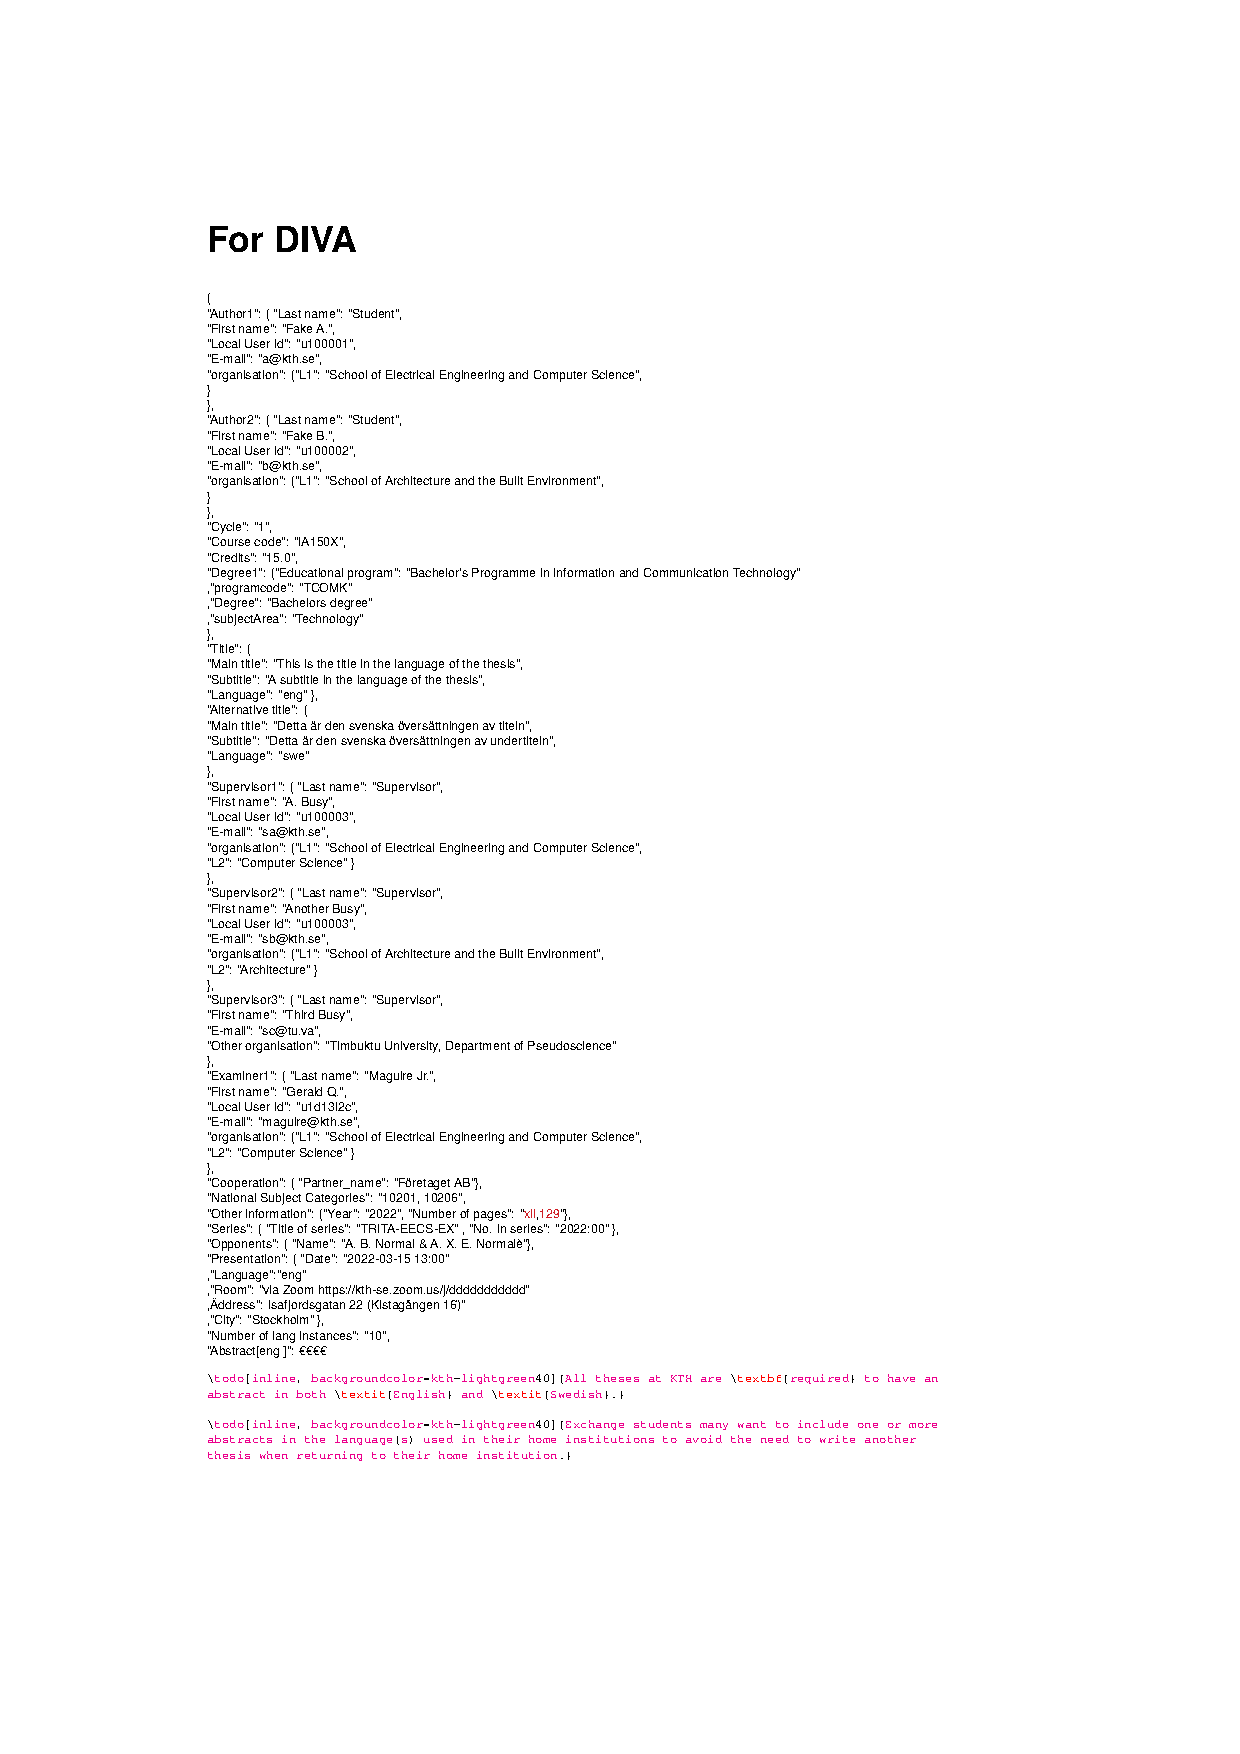
\includegraphics[width=0.85\textwidth]{README_notes/README-examiner-figures/ForDIVA-pg1.pdf}}
  \end{center}
  \caption{First page of the “For DiVA” information}
  \label{fig:sampleFOrDIVApage1}
\end{figure}
\clearpage
\begin{lstlisting}[language={json}, caption={Text version of the first page of the For DIVA output}, label=lst:forDIVApg11Text]
{
"Author1": { "Last name": "Student",
"First name": "Fake A.",
"Local User Id": "u100001",
"E-mail": "a@kth.se",
"organisation": {"L1": "School of XXX",
}
},
"Author2": { "Last name": "Student",
"First name": "Fake B.",
"Local User Id": "u100002",
"E-mail": "b@kth.se",
"organisation": {"L1": "School of XXX",
}
},
"Cycle": "1",
"Course code": "XX100X",
"Credits": "15.0",
"Degree1": {"Educational program": "Bachelor’s Programme in XXX"
,"programcode": "TCOMK"
,"Degree": "Bachelors degree"
,"subjectArea": "Technology"
},
"Title": {
"Main title": "This is the title in the language of the thesis",
"Subtitle": "A subtitle in the language of the thesis",
"Language": "eng" },
"Alternative title": {
"Main title": "Detta är den svenska översättningen av titeln",
"Subtitle": "Detta är den svenska översättningen av undertiteln",
"Language": "swe"
},
"Supervisor1": { "Last name": "Supervisor",
"First name": "A. Busy",
"Local User Id": "u100003",
"E-mail": "sa@kth.se",
"organisation": {"L1": "School of XXX",
"L2": "DepartmentName" }
},
"Supervisor2": { "Last name": "Supervisor",
"First name": "Another Busy",
"Local User Id": "u100003",
"E-mail": "sb@kth.se",
"organisation": {"L1": "School of XXX",
"L2": "DepartmentName" }
},
"Supervisor3": { "Last name": "Supervisor",
"First name": "Third Busy",
"E-mail": "sc@tu.va",
"Other organisation": "Timbuktu University, Department of Pseudoscience"
},
"Examiner1": { "Last name": "ExaaminersLastname",
"First name": "ExaaminersFistname",
"Local User Id": "u1000000",
"E-mail": "xxx@kth.se",
"organisation": {"L1": "School of XXX",
"L2": "DepartmentName" }
},
"Cooperation": { "Partner_name": "Företaget AB"},
"National Subject Categories": "ddddd, ddddd",
"Other information": {"Year": "2022", "Number of pages": "xli,133"},
"Series": { "Title of series": "TRITA-XXX-EX" , "No. in series": "2022:00" },
"Opponents": { "Name": "A. B. Normal & A. X. E. Normalè"},
"Presentation": { "Date": "2022-03-15 13:00"
,"Language":"eng"
,"Room": "via Zoom https://kth-se.zoom.us/j/ddddddddddd"
,"Äddress": Isafjordsgatan 22 (Kistagången 16)"
,"City": "Stockholm" },
"Number of lang instances": "10",
"Abstract[eng ]": €€€€
\engExpl{All theses at KTH are \textbf{required} to have an
abstract in both \textit{English} and \textit{Swedish}.}
\engExpl{Exchange students many want to include one or more
abstracts in the language(s) used in their home institutions to avoid the need to write another
thesis when returning to their home institution.}
\end{lstlisting}
\clearpage
\begin{figure}[!ht]
  \begin{center}
    \fbox{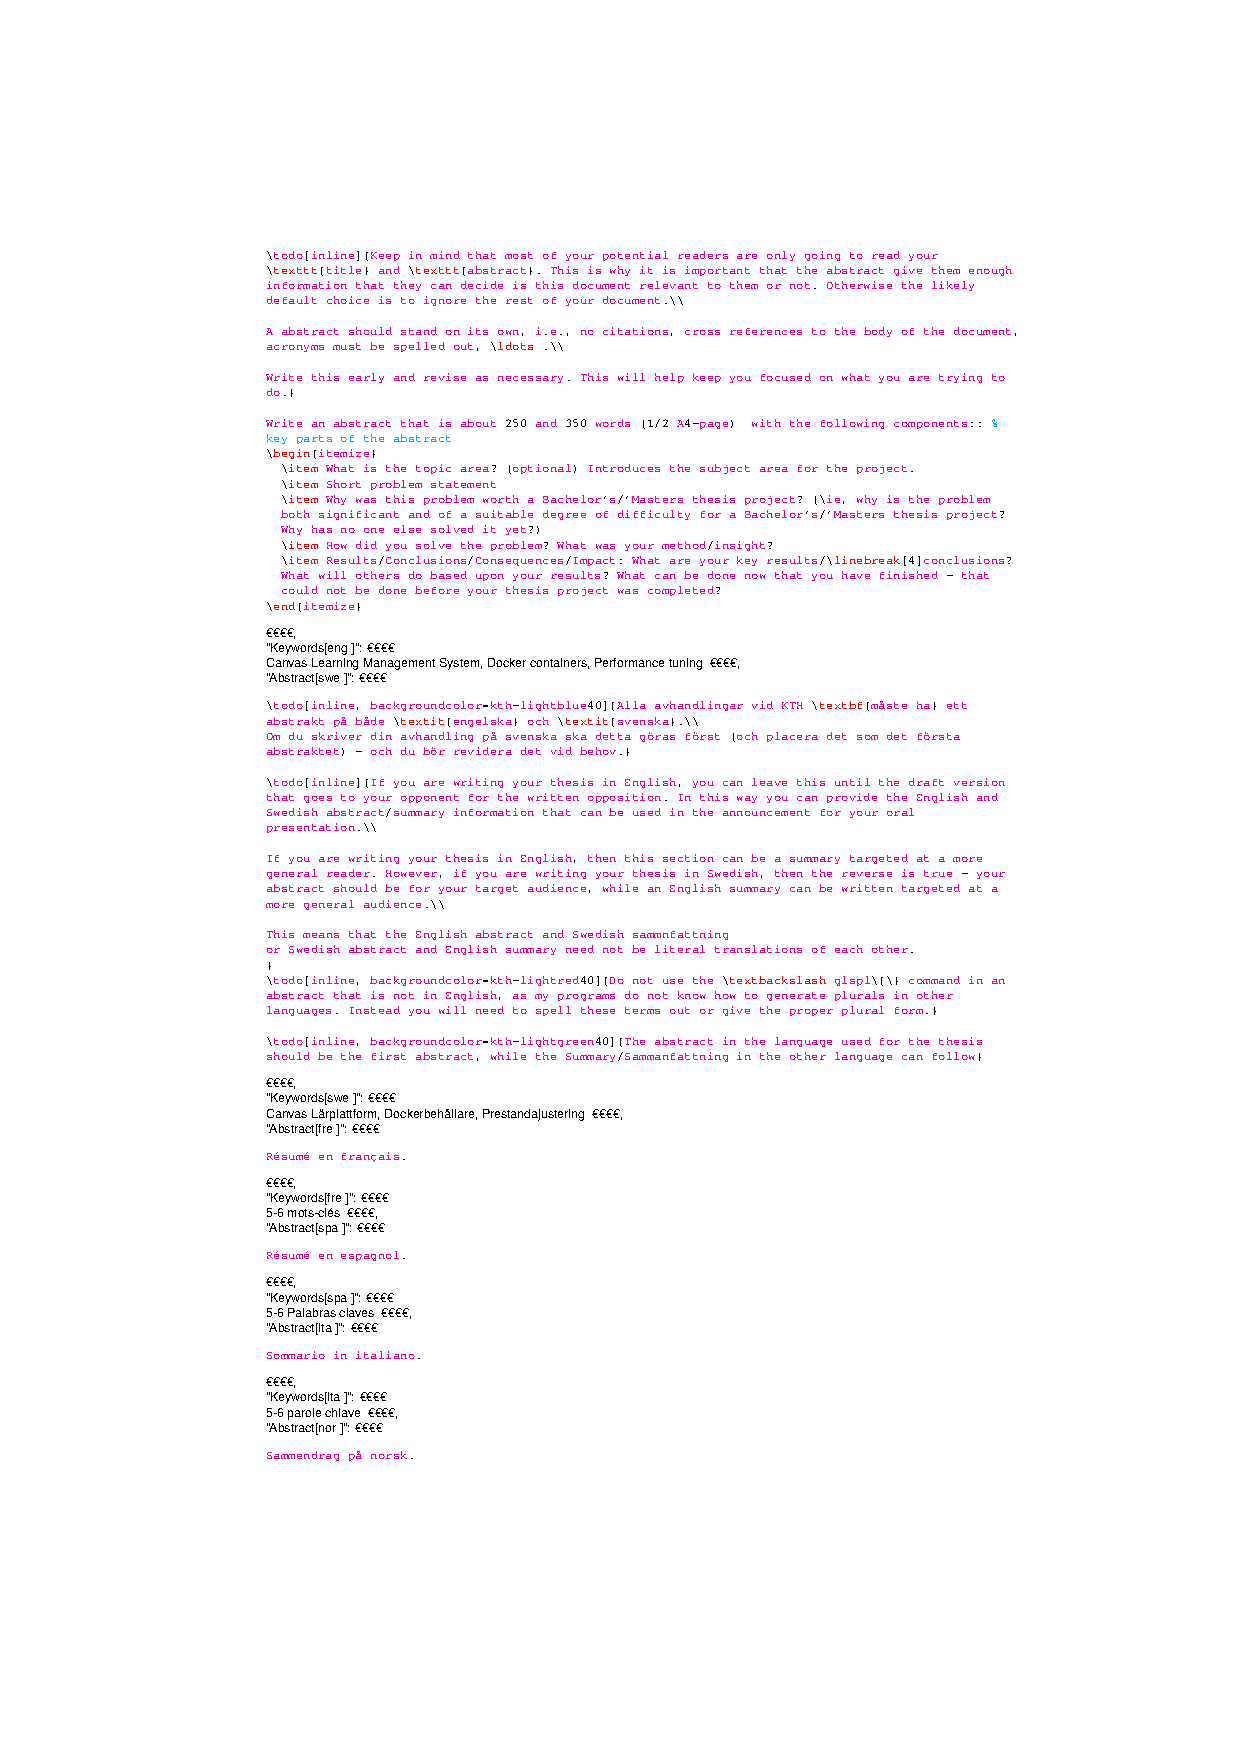
\includegraphics[width=0.80\textwidth]{README_notes/README-examiner-figures/ForDIVA-pg2.pdf}}
  \end{center}
  \caption{Second page of the “For DiVA” information}
  \label{fig:sampleFOrDIVApage2}
\end{figure}
\begin{figure}[!ht]
  \begin{center}
    \fbox{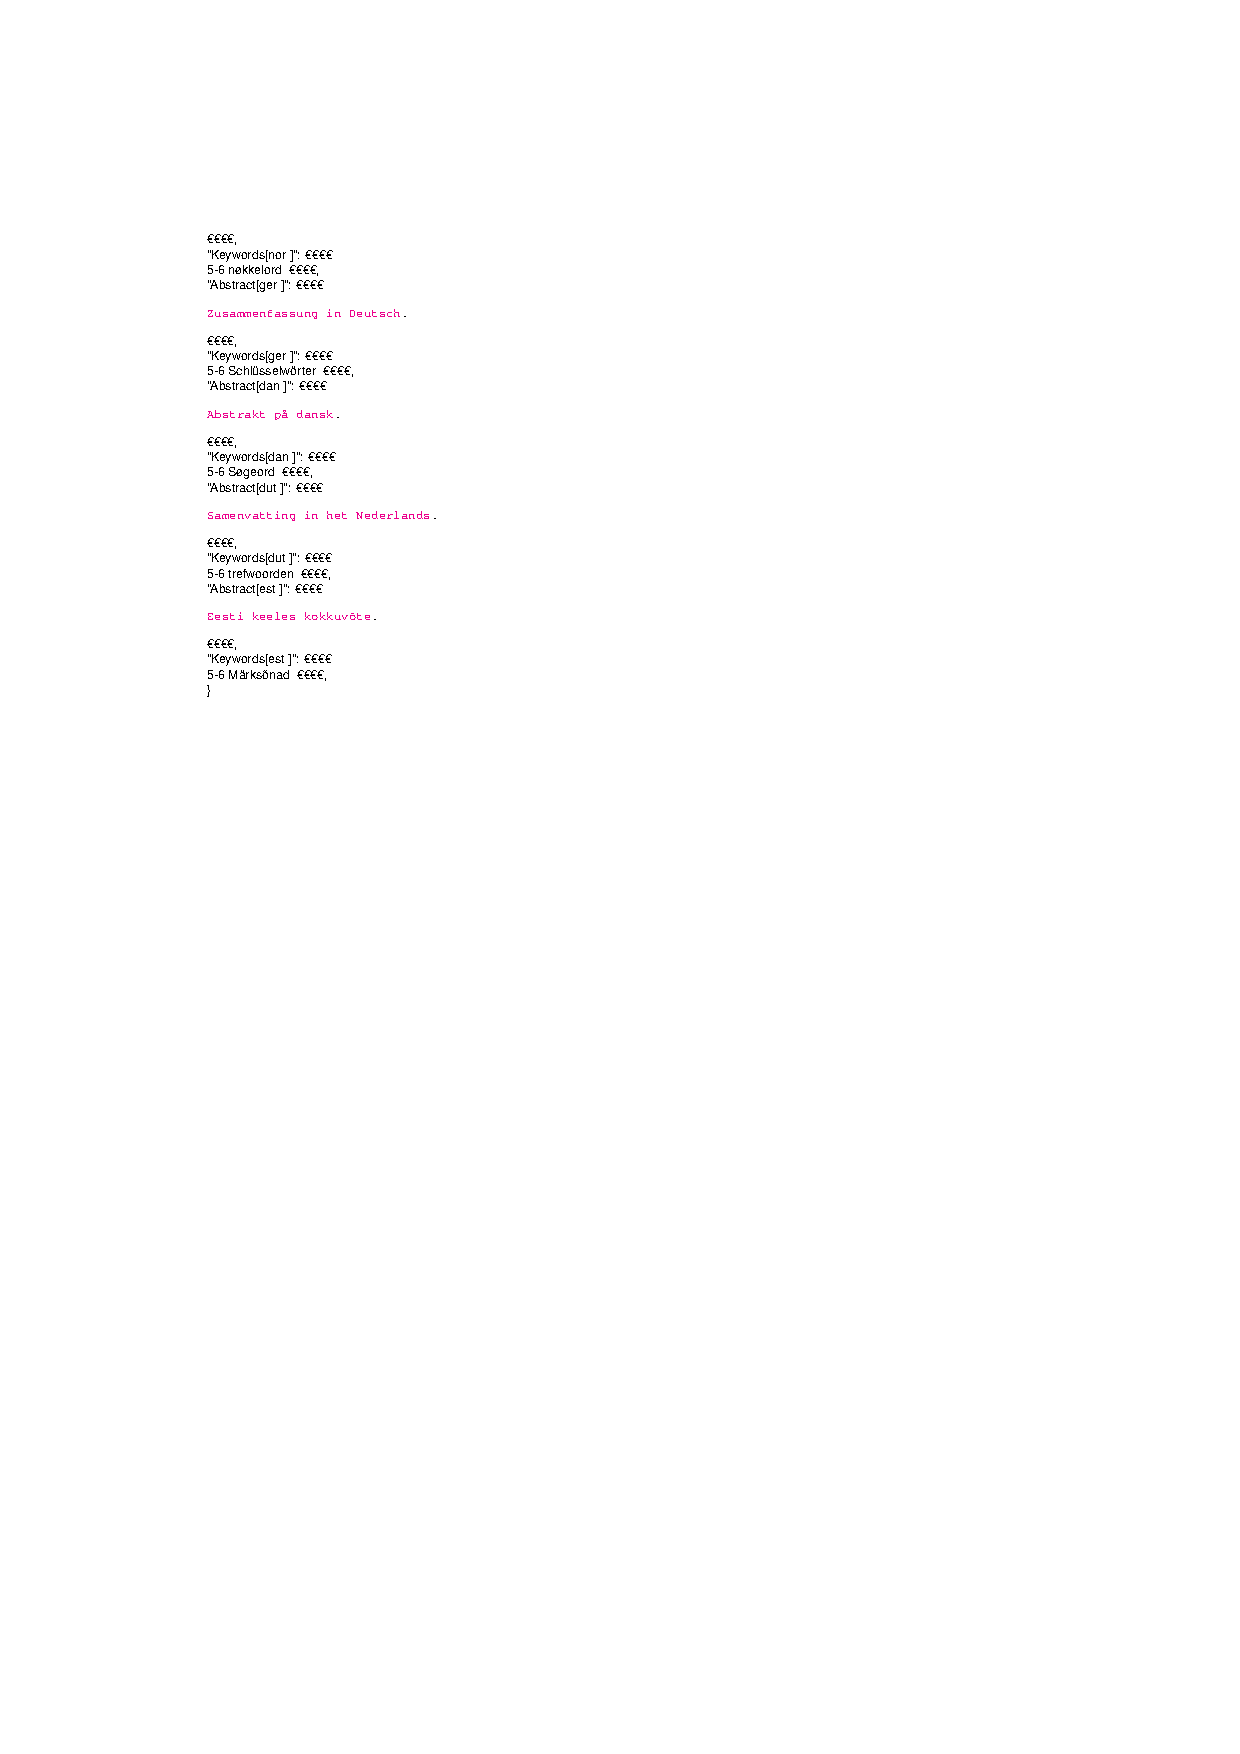
\includegraphics[width=0.80\textwidth]{README_notes/README-examiner-figures/ForDIVA-pg3.pdf}}
  \end{center}
  \caption{Third page of the “For DiVA” information}
  \label{fig:sampleFOrDIVApage3}
\end{figure}
\clearpage
\FloatBarrier


\section{How did the abstracts and the keywords appear?}
\label{sec:scontentsHack}
The \textbackslash divainfo command that generates the For DiVA information pages has the following little bit of code that walks the set of scontents buffers using the lang scontents buffer to put the language and the corresponding abstract and keywords (see \Cref{lst:languages}). Originally, I used \textbackslash getstored[\textbackslash i]{abstracts} to get an abstract, but this turns out to process the \LaTeX~into something to render in the PDF. However, I realized that it would be far better to get the actual \LaTeX~source code and then process it myself into HTML for the announcement and calendars.

The \textbackslash typestored command that the scontents package provides will not take a variable argument, \ie it only takes a constant, such as \textbackslash typestored[2]{abstracts}. Unfortunately, I need to have a loop to handle the variable number of abstracts that could be used. To do this required a new command \textbackslash typestoredx that evaluates the variable and then calls the internal function that gets the contents of the correct scontents buffer! This new command is shown in \Cref{lst:languages} – it uses ExplSyntax – see the \LaTeX~package \texttt{expl3}. The quad euro symbols are used as markers to avoid problems with quotation marks in the abstract itself. I have assumed that such a combination of characters will \textbf{never} occur in an abstract.
\Needspace*{11\baselineskip}
\begin{lstlisting}[language={[LaTeX]TeX}, caption={Code in \textbackslash divainfo command to output the abstracts and keywords }, label=lst:languages] 
    "Number of lang instances": \textquotedbl\relax\countsc{lang}\textquotedbl\relax,\\
    \foreach \i in {1,...,\countsc{lang}} {
      "Abstract[\getstored[\i]{lang}]": €€€€\\
      \typestoredx{\i}{abstracts}
      €€€€,\\
      "Keywords[\getstored[\i]{lang}]": €€€€\\
      \getstored[\i]{keywords}
      €€€€,\\
    }
\end{lstlisting}

\Cref{lst:setupTypestoreedx} shows how to configure the listings environment to put the abstract into. One of the tricks here is that it was important to reduce the hyphenation penalty to enable the abstract text to nicely wrap text on the page. As an added benefit, the \LaTeX~syntax highlighting is on – so one can easily see the \LaTeX~commands that are used – as they might need manual editing before the event is announced. The \LaTeX~code for the English and Swedish abstracts is shown in \Cref{lst:latexAbtractsExampleEnglish} and \Cref{lst:latexAbtractsExampleSwedish} (respectively).

\begin{lstlisting}[language={[LaTeX]TeX}, caption={Code in the document file to set up the command \textbackslash typestoredx and to configure the listing environment to put the abstract into}, label=lst:setupTypestoreedx] 
\ExplSyntaxOn
\newcommand\typestoredx[2]{\expandafter\__scontents_typestored_internal:nn\expandafter{#1} {#2}}
\ExplSyntaxOff
\makeatletter
\let\verbatimsc\@undefined
\let\endverbatimsc\@undefined
\lst@AddToHook{Init}{\hyphenpenalty=50\relax}
\makeatother


\lstnewenvironment{verbatimsc}
    {
    \lstset{%
        basicstyle=\ttfamily\tiny,
        %basicstyle=\tiny,
        %columns=fullflexible,
        columns=[l]fixed,
        language=[LaTeX]TeX,
        %numbers=left,
        %numberstyle=\tiny\color{gray},
        keywordstyle=\color{red},
        breaklines=true,                 % sets automatic line breaking
        breakatwhitespace=true,          % sets if automatic breaks should only happen at whitespace
        %keepspaces=false,
        breakindent=0em,
        %fancyvrb=true
    }
}{}
\end{lstlisting}
\clearpage

\begin{lstlisting}[language={[LaTeX]TeX}, caption={\LaTeX~code for the English abstract}, label=lst:latexAbtractsExampleEnglish] 
\engExpl{All theses at KTH are \textbf{required} to have an
abstract in both \textit{English} and \textit{Swedish}.}
\engExpl{Exchange students many want to include one or more
abstracts in the language(s) used in their home institutions to avoid the need to write another
thesis when returning to their home institution.}
\generalExpl{Keep in mind that most of your potential readers are only going to read your
\texttt{title} and \texttt{abstract}. This is why it is important that the abstract give them enough
information that they can decide if this document is relevant to them or not. Otherwise, the likely
default choice is to ignore the rest of your document.\\
An abstract should stand on its own, i.e., no citations, cross-references to the body of the document,
acronyms must be spelled out, \ldots .\\
Write this early and revise as necessary. This will help keep you focused on what you are trying to
do.}
Write an abstract that is about 250 and 350 words (1/2 A4-page) with the following components:: %
key parts of the abstract
\begin{itemize}
\item What is the topic area? (optional) Introduces the subject area for the project.
\item Short problem statement
\item Why was this problem worth a Bachelor’s/’Masters thesis project? (\ie, why is the problem
both significant and of a suitable degree of difficulty for a Bachelor’s/’Masters thesis project?
Why has no one else solved it yet?)
\item How did you solve the problem? What was your method/insight?
\item Results/Conclusions/Consequences/Impact: What are your key results/\linebreak[4]conclusions?
What will others do based on your results? What can be done now that you have finished - that
could not be done before your thesis project was completed?
\end{itemize}
\end{lstlisting}

\begin{lstlisting}[language={[LaTeX]TeX}, caption={\LaTeX~code for the Swedish abstract}, label=lst:latexAbtractsExampleSwedish]
\todo[inline, backgroundcolor=kth-lightblue40]{Alla avhandlingar vid KTH \textbf{måste ha} ett
abstrakt på både \textit{engelska} och \textit{svenska}.\\
Om du skriver din avhandling på svenska ska detta göras först (och placera det som det första
abstraktet) - och du bör revidera det vid behov.}
\generalExpl{If you are writing your thesis in English, you can leave this until the draft version
that goes to your opponent for the written opposition. In this way you can provide the English and
Swedish abstract/summary information that can be used in the announcement for your oral
presentation.\\
If you are writing your thesis in English, then this section can be a summary targeted at a more
general reader. However, if you are writing your thesis in Swedish, then the reverse is true – your
abstract should be for your target audience, while an English summary can be written targeted at a
more general audience.\\
This means that the English abstract and Swedish sammnfattning
or Swedish abstract and English summary need not be literal translations of each other.
}
\warningExpl{Do not use the \textbackslash glspl\{\} command in an
abstract that is not in English, as my programs do not know how to generate plurals in other
languages. Instead you will need to spell these terms out or give the proper plural form.}
\engExpl{The abstract in the language used for the thesis
should be the first abstract, while the Summary/Sammanfattning in the other language can follow}
\end{lstlisting}

\section{Extracting the information from the PDF file}
Now that the JSON-like information is in the PDF file, the next step is to extract it. The command line shown in \Cref{lst:extractPseudoJSONfromPDF-event} will extract the information. \Cref{lst:JSONfromPDF-event} shows an example of the resulting file.
\begin{lstlisting}[language={bash}, caption={Extract the JSON like information}, label=lst:extractPseudoJSONfromPDF-event]
./extract_pseudo_JSON-from_PDF.py --pdf test5.pdf --json event.json
\end{lstlisting}

\begin{lstlisting}[language={HTML}, caption={Example event.json output (note that this is not the same as currently extracted and note that some lines have been edited and manually broken to overcome limited line length in listing)}, label=lst:JSONfromPDF-event]
{"Author1": {"Last name": "Student", "First name": "Fake A.", "Local User Id": "u100001", "E-mail": "a@kth.se", "organisation": {"L1": "School of XXX"}},
"Author2": {"Last name": "Student", "First name": "Fake B.", "Local User Id": "u100002", "E-mail": "b@kth.se", "organisation": {"L1": "XXX"}},
"Degree": {"Educational program": "Bachelor’s Programme in XXX"},
"Title": {"Main title": "This is the title in the language of the thesis", "Subtitle": "An subtitle in the language of the thesis", "Language": "eng"},
"Alternative title": {"Main title": "Detta är den svenska översättningen av titeln", "Subtitle": "Detta är den svenska översättningen av undertiteln", "Language": "swe"},
"Supervisor1": {"Last name": "Supervisor", "First name": "A. Busy", "Local User Id": "u100003", "E-mail": "sa@kth.se", "organisation": {"L1": "School of XXX", "L2": "DepartmentName"}},
"Supervisor2": {"Last name": "Supervisor", "First name": "Another Busy", "Local User Id": "u100003", "E-mail": "sb@kth.se", "organisation": {"L1": "School of XXX", "L2": "DepartmentName"}},
"Examiner1": {"Last name": "ExaminersLastname", "First name": "ExaminersLastname", "Local User Id": "u100004", "E-mail": "xxx@kth.se", "organisation": {"L1": "School of EXXX", "L2": "DepartmentName"}},
"Cooperation": {"Partner_name": "Företaget AB"}, "Other information": {"Year": "2021", "Number of pages": "xxxiii,35"},
"Opponents": {"Name": "A. B. Normal & A. X. E. Normalè"},
"Presentation": {"Date": "2021-03-16 13:00", "Language": "eng", "Room": "via Zoom", "City": "Stockholm"},
"Number of lang instances": "10",
"abstracts": {"eng": "<p>All theses at KTH are <bold>required</bold> to have an abstract in both <i>English</i> and <i>Swedish</i>.</p><p>Exchange students many want to include one or more abstracts in the language(s) used in their home institutions to avoid the need to write another thesis when returning to their home institution.</p><p>Keep in mind that most of your potential readers are only going to read your <tt>title</tt> and <tt>abstract</tt>. This is why it is important that the abstract give them enough information that they can decide is this document relevant to them or not. Otherwise the likely default choice is to ignore the rest of your document.</p><p>A abstract should stand on its own, i.e., no citations, cross references to the body of the document, acronyms must be spelled out, … .</p><p>Write this early and revise as necessary. This will help keep you focused on what you are trying to do.</p><p>Example of a formula in an abstract: $c=2 \\cdot \\pi \\cdot r$ or \\[ \\int_{a}^{b} x^2 \\,dx \\] two chemical formulas: H<sub>2</sub>O or $(C_5O_2H_8)_n$, copyright symbol: &copy; Maguire 2021, and some superscripts: <sup>99m</sup>Tc, A<sup>*</sup>, A<sup>&reg;</sup>, and A&trade;.</p><p>Write an abstract with the following components: </p><ul><li> What is the topic area? (optional) Introduces the subject area for the project. </li><li> Short problem statement </li><li> Why was this problem worth a ’Masters thesis project? (i.e., why is the problem both significant and of a suitable degree of difficulty for a ’Masters thesis project? Why has no one else solved it yet?) </li><li> How did you solve the problem? What was your method/insight? </li><li> Results/Conclusions/Consequences/Impact: What are your key results/conclusions? What will others do based upon your results? What can be done now that you have finished - that could not be done before your thesis project was completed?</li></ul>",
"swe": "<p>Alla avhandlingar vid KTH måste ha ett abstrakt på både engelska och svenska.</p><p>If you are writing your thesis in English, you can leave this until the final version. If you are writing your thesis in Swedish then this should be done first – and you should revise as necessary along the way.</p><p>If you are writing your thesis in English, then this section can be a summary targeted at a more general reader. However, if you are writing your thesis in Swedish, then the reverse is true – your abstract should be for your target audience, while an English summary can be written targeted at a more general audience.</p><p>This means that the English abstract and Swedish sammnfattning or Swedish abstract and English summary need not be literal translations of each other.</p><p>The abstract in the language used for the thesis should be the first abstract, while the Summary/Sammanfattning in the other language can follow.</p>",
"fre": "<p>Résumé en français.</p>", "spa": "<p>Résumé en espagnol.</p>", "ita": "<p>Sommario in italiano.</p>",
"nor": "<p>Sammendrag på norsk.</p>", "ger": "", "dan": "<p>Abstrakt på dansk.</p><p>Zusammenfassung in Deutsch.</p>",
"dut": "<p>Samenvatting in het Nederlands.</p><p>Eesti keeles kokkuvõte.</p>", "est": ""},
"keywords": {"eng": "Canvas Learning Management System, Docker containers, performance tuning ",
"swe": "Canvas Lärplattform,Dockerbehållare, prestandajustering ", "fre": "5-6 mots-clés ",
"spa": "5-6 Palabras claves ", "ita": "5-6 parole chiave ", "nor": "5-6 nøkkelord ",
"ger": "5-6 Schlüsselwörter ", "dan": "5-6 Søgeord ",
"dut": "5-6 trefwoorden ", "est": "5-6 Märksõnad "}}
\end{lstlisting}
\FloatBarrier

\section{Optimized extraction from an Overleaf LaTeX project}
\label{sec:optimizeJSONToMods}
In the case of an Overleaf project, when compiling the \LaTeX~\ as a side-effect, a \texttt{fordiva.json} file is generated, if you save this file locally, then you can clean it up and make a MODS file with the following commands:
\Needspace*{4\baselineskip}
\begin{lstlisting}[language={bash}, caption={cleanup\_pseudo\_JSON-from\_LaTeX and JSON\_to\_MODS.p},label=lst:cleanPseudoJSONandConvertToMODS]
./cleanup_pseudo_JSON-from_LaTeX.py --json xxx_fordiva.json --acronyms acronyms.tex
./JSON_to_MODS.py --json xxx_fordiva.json
\end{lstlisting}

Now all you have to do is rename the XML file that was produced to \texttt{xxx.mods} and you are all set to upload it into DiVA!

To find the \texttt{fordiva.json} file, look for the “Other logs and files” button shown at the bottom of the log output window. This button is shown in \Cref{fig:otherLogfiles}. After clicking this button you will see a list of log and other files, such as shown in \ref{fig:filesProduced}.
	
\begin{figure}[!ht]
  \begin{center}
    \fbox{
\includegraphics[width=0.80\textwidth]{README_notes/README-examiner-figures/otherlog_files.png}}
  \end{center}
  \caption{Other logs and files button}
  \label{fig:otherLogfiles}
\end{figure}

The details for how the \texttt{fordiva.json} file is generated are given in \Cref{sec:AlternativeWayofGeneratingJSON}.

 \begin{figure}[!ht]
  \begin{center}
    \fbox{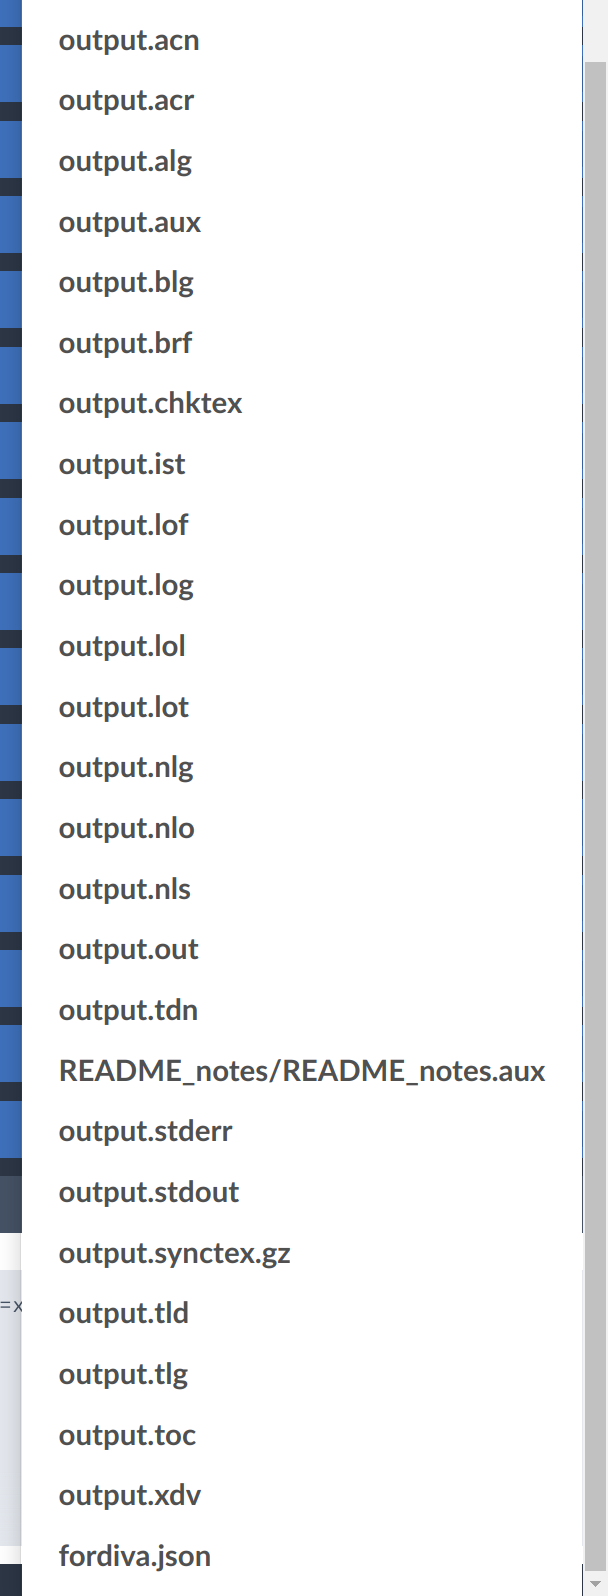
\includegraphics[width=0.50\textwidth]{README_notes/README-examiner-figures/files-produced-Screenshot_20220326_181731.png}}
  \end{center}
  \caption{List of log and other files}
  \label{fig:filesProduced}
\end{figure}
\clearpage

\section{What can we do with the JSON file?}
\label{sec:whatCanweDoWithTheJSONfile}
Now that we have a JSON file, you can edit the HTML in the abstracts to deal with equations and things that were not automatically processed by the extraction program. Once you are happy with the JSON file’s contents, the next step is to generate something interesting with this data – for this we use the program JSON\_to\_calendar.py. 



 \begin{figure}[!ht]
\begin{tikzpicture}
[align=left,node distance=2cm]
\node (jsonFile) [tape,tape bend top=none,draw,font=\sffamily] {JSON file};
\node (start) [processBox, right=1cm of jsonFile] {JSON\_to\_calendar};

\node (calendarEvent) [destinationBox, right=2cm of start] {Canvas calendar event};
\node (announcement) [destinationBox,  above of =calendarEvent] {Canvas announcement};
\node (cortinaCalendarEvent) [destinationBox,  right=0.5cm of start, below of=calendarEvent] {KTH Cortina calendar event};
\draw [arrow] (jsonFile) --  (start.west);
\draw [arrow] (start.east) --  (announcement.west);
\draw [arrow] (start.east) -- (calendarEvent);
\draw [arrow] (start.east) -- (cortinaCalendarEvent.west);

\end{tikzpicture}
\caption{The several outputs of JSON\_to\_calendar.py given a JSON file}
  \label{fig:foo}
\end{figure}
\FloatBarrier

We can produce all three outputs with the command shown in \Cref{lst:JSONtoCalendarThreeoutputs}. Note that the program was run with the \texttt{event.json} file to produce a Canvas course announcement, as shown in \Cref{fig:canvasCourseAnnouncement}. Note that this is being run in the Canvas test instance (hence the pink bar across the bottom of the figure).
\Needspace*{3\baselineskip}
\begin{lstlisting}[language={bash}, caption={Running JSON\_to\_calendar.py to produce all three outputs}, label=lst:JSONtoCalendarThreeoutputs]
JSON_to_calendar.py -c 11 --config config-test.json
\end{lstlisting}

When the cover generator website existed, this same basic mechanism was extended to make and apply the cover for a thesis. There is still a need for a tool that can automate the insertion of the final thesis and metadata into DiVA. While a prototype was shown earlier for this, the IT unit wants to wait for a DiVA API from the DiVA organization. However, an alternative is to generate a MODS file that can be manually imported into DiVA. The process for this will be discussed in \Cref{sec:JSONtoMODSfile}.
\clearpage
\begin{figure}[!ht]
  \begin{center}
    \fbox{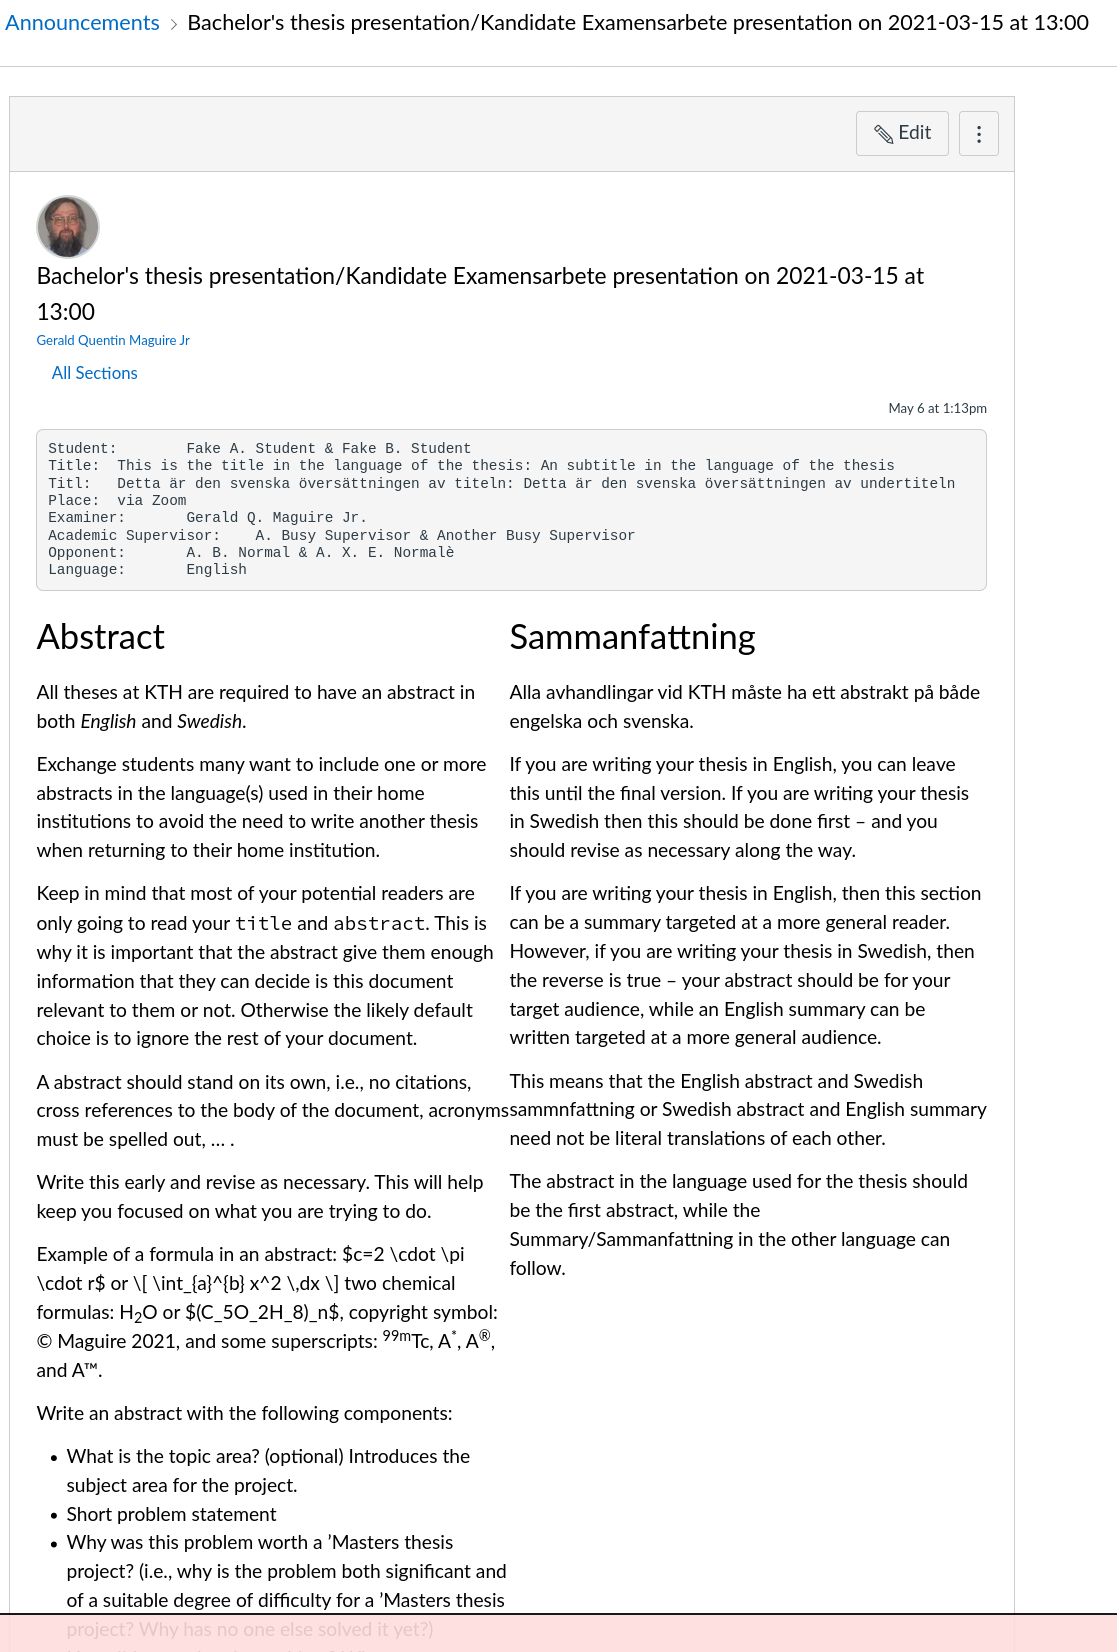
\includegraphics[width=0.99\textwidth]{README_notes/README-examiner-figures/Announcement-in-Canvas-course-Screenshot_20210506_133101.png}}
  \end{center}
  \caption{Canvas course announcement}
  \label{fig:canvasCourseAnnouncement}
\end{figure}
\clearpage
\Cref{fig:canvasCourseAnnouncement} and \Cref{fig:canvasCalendarEvent}  show the event in the Canvas calendar (when I have selected to display the events for course 11 in green).
\begin{figure}[!ht]
  \begin{center}
    \fbox{
\includegraphics[width=0.60\textwidth]{README_notes/README-examiner-figures/Event-in-Canvas-course-calendar-Screenshot_20210506_133011.png}}
  \end{center}
  \caption{A course event in the Canvas calendar (the figure is zoomed in on 15 March 2021}
  \label{fig:canvasCalendarEvent}
\end{figure}

\begin{figure}[!hb]
  \begin{center}
    \fbox{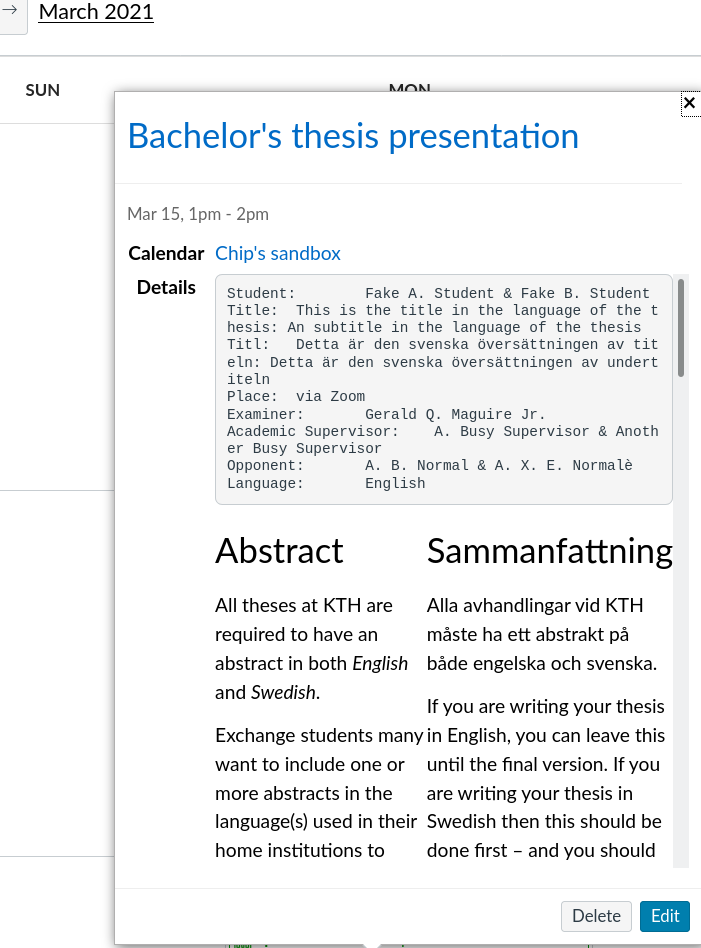
\includegraphics[width=0.70\textwidth]{README_notes/README-examiner-figures/Canvas-calenda-zoomed-open-event-Screenshot_20210506_163851.png}}
  \end{center}
  \caption{Zoomed view of the opened Canvas calendar event}
  \label{fig:canvasCalendarEventZoomed}
\end{figure}
\newpage

I also edited the \texttt{event.json} to create an event on the following date. The result is two Calendar events as shown in \Cref{fig:cortinaPicture1} in KTH’s Cortina calendar (in this case, it is in the development version of the Polopoly web – as this is the only place where I can use the as of yet unreleased Cortina API which is being developed by KTH’s IT unit. \Cref{fig:cortinaPicture2} and \Cref{fig:cortinaPicture3} show the English and Swedish versions of the event in the calendar.s

\begin{figure}[!ht]
  \begin{center}
    \fbox{
\includegraphics[width=0.99\textwidth, trim=3cm 2cm 8cm 0.2cm, clip]{README_notes/README-examiner-figures/cortina-2021-03-16-picture.png}}
  \end{center}
  \caption{KTH’s Cortina calendar showing two degree project events}
  \label{fig:cortinaPicture1}
\end{figure}
\FloatBarrier

\begin{figure}[!ht]
  \begin{center}
    \fbox{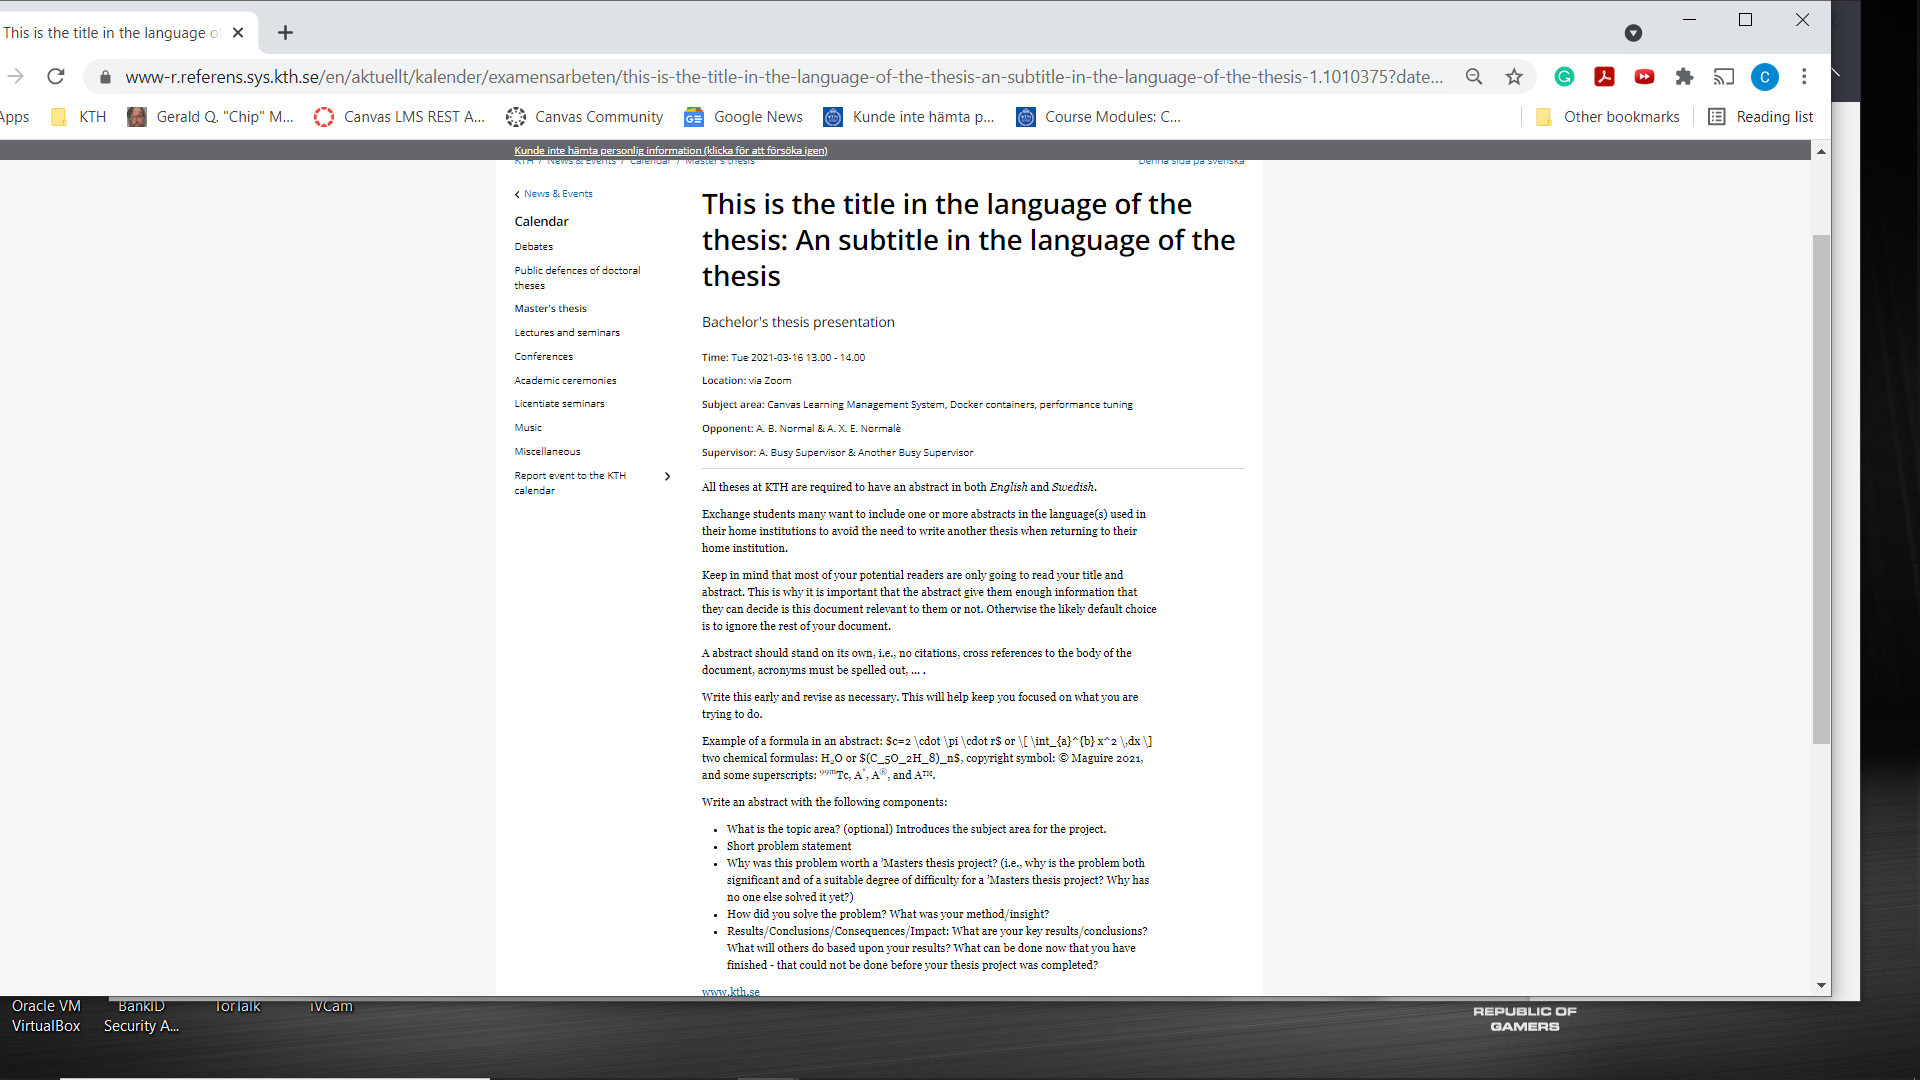
\includegraphics[width=1.0\textwidth, trim=3cm 2cm 16cm 0.2cm, clip]{README_notes/README-examiner-figures/cortina-2021-03-16-picture2.png}}
  \end{center}
  \caption{English version of the calendar}
  \label{fig:cortinaPicture2}
\end{figure}
\FloatBarrier	

\begin{figure}[!ht]
  \begin{center}
    \fbox{
\includegraphics[width=1.0\textwidth, trim=3cm 2cm 16cm 0.2cm, clip]{README_notes/README-examiner-figures/cortina-2021-03-16-picture3.png}}
  \end{center}
  \caption{Swedish version of the calendar}
  \label{fig:cortinaPicture3}
\end{figure}
\FloatBarrier

\Cref{lst:cortinaResponse} shows the response from doing a POST to the KTH Cortina API. Note that this is a prototype and as of the date of my experiments did not yet support having an examiner in a calendar event (hence I had to save and remove this element of the dict before passing the data to the API, then I restored this element for use by the subsequent routines).

\begin{lstlisting}[language={json}, caption={Response from the KTH Cortina API},label=lst:cortinaResponse]
{
  "advisor": "A. Busy Supervisor & Another Busy Supervisor",
  "contentId": "1.1010375",
  "contentName": {
    "en_GB": "This is the title in the language of the thesis: An subtitle in the language of the thesis",
    "sv_SE": "Detta är den svenska översättningen av titeln: Detta är den svenska översättningen av undertiteln"
  },
  "dates_endtime": "2021-03-16T13:00:00.000Z",
  "dates_starttime": "2021-03-16T12:00:00.000Z",
  "lead": {
    "en_GB": "Bachelor's thesis presentation",
    "sv_SE": "Kandidate Examensarbete presentation"
  },
  "lecturer": "Fake A. Student & Fake B. Student",
  "location": "via Zoom",
  "opponent": "A. B. Normal & A. X. E. Normalè",
  "organisation": {
    "school": "XXX",
    "department": "DepartmentName"
  },
  "respondent": "",
  "respondentDepartment": "",
  "subjectarea": {
    "en_GB": "KeywordA, KeywordB, KeywordC",
    "sv_SE": "NyckelordA, NyckelordB, NyckelordC"
  },
  "seminartype": "thesis",
  "paragraphs_text": {
    "en_GB": "<p>All theses at KTH are required to have an abstract in both <i>English</i> and <i>Swedish</i>.</p> \n<p>Exchange students many want to include one or more abstracts in the language(s) used in their home institutions to avoid the need to write another thesis when returning to their home institution.</p> \n<p>Keep in mind that most of your potential readers are only going to read your title and abstract. This is why it is important that the abstract give them enough information that they can decide is this document relevant to them or not. Otherwise the likely default choice is to ignore the rest of your document.</p> \n<p>A abstract should stand on its own, i.e., no citations, cross references to the body of the document, acronyms must be spelled out, … .</p> \n<p>Write this early and revise as necessary. This will help keep you focused on what you are trying to do.</p> \n<p>Example of a formula in an abstract: $c=2 \\cdot \\pi \\cdot r$ or \\[ \\int_{a}^{b} x^2 \\,dx \\] two chemical formulas: H<sub>2</sub>O or $(C_5O_2H_8)_n$, copyright symbol: © Maguire 2021, and some superscripts: <sup>99m</sup>Tc, A<sup>*</sup>, A<sup>®</sup>, and A™.</p> \n<p>Write an abstract with the following components: </p> \n<ul> \n <li> What is the topic area? (optional) Introduces the subject area for the project. </li> \n <li> Short problem statement </li> \n <li> Why was this problem worth a ’Masters thesis project? (i.e., why is the problem both significant and of a suitable degree of difficulty for a ’Masters thesis project? Why has no one else solved it yet?) </li> \n <li> How did you solve the problem? What was your method/insight? </li> \n <li> Results/Conclusions/Consequences/Impact: What are your key results/conclusions? What will others do based upon your results? What can be done now that you have finished - that could not be done before your thesis project was completed?</li> \n</ul>\n",
    "sv_SE": "<p>Alla avhandlingar vid KTH måste ha ett abstrakt på både engelska och svenska.</p> \n<p>If you are writing your thesis in English, you can leave this until the final version. If you are writing your thesis in Swedish then this should be done first – and you should revise as necessary along the way.</p> \n<p>If you are writing your thesis in English, then this section can be a summary targeted at a more general reader. However, if you are writing your thesis in Swedish, then the reverse is true – your abstract should be for your target audience, while an English summary can be written targeted at a more general audience.</p> \n<p>This means that the English abstract and Swedish sammnfattning or Swedish abstract and English summary need not be literal translations of each other.</p> \n<p>The abstract in the language used for the thesis should be the first abstract, while the Summary/Sammanfattning in the other language can follow.</p>\n"
  },
  "uri": "https://www.kth.se"
}
\end{lstlisting}


\section{Actual example}
This example appears with the student’s permission. \Cref{fig:actualAnnouncementTop} shows the announcement for a second-cycle thesis presentation in a Canvas course while \Cref{fig:actualAnnouncementBottom} shows the bottom part of the announcement. \Cref{fig:actualCalendarOpenned} shows the opened Canvas course calendar entry while \Cref{fig:actualEnglishAndSwedish} shows the Cortina calendar entry. Note that the Cortina calendar entry is in the development system and not the production calendar. \Cref{lst:extractPseudoAndJSONtoCalendar} shows the command to extract the JSON information from the student’s PDF file and then the command to make the announcement and calendar entries. \Cref{lst:extractedPseudoAndJSONtoCalendar} shows the extracted JSON.

Note that the entry was made on 2021-06-17, but the event was earlier. This entry was made with the new (as of this date) KTH Cortina Calendar API that supports the examiner and language of presentation fields. Additionally, it returns a canonicalUrl (the URL to this calendar entry). The program was extended to add this URL to the course announcement and course calendar entry.

\begin{figure}[!ht]
  \begin{center}
    \fbox{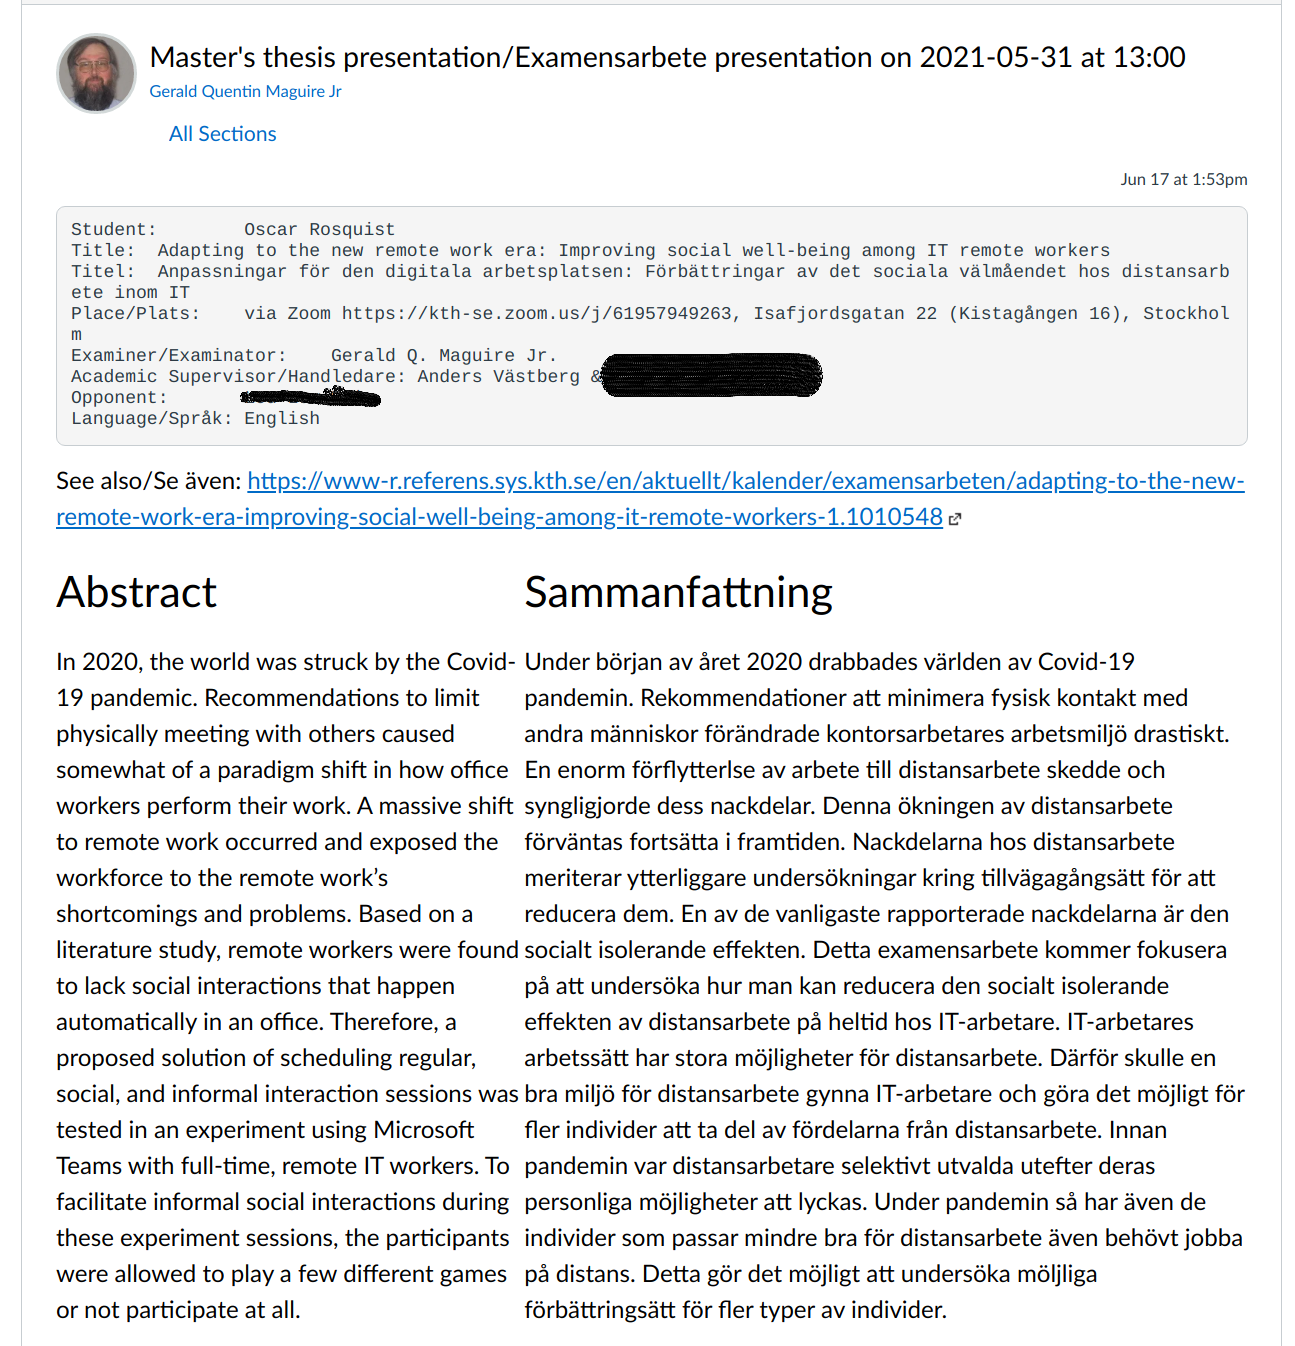
\includegraphics[width=1.2\textwidth]{README_notes/README-examiner-figures/Oscar-1-Screenshot_20210617_140037.png}}
  \end{center}
  \caption{Actual example of announcement in Canvas (top)}
  \label{fig:actualAnnouncementTop}
\end{figure}
\FloatBarrier

\begin{figure}[!ht]
  \begin{center}
    \fbox{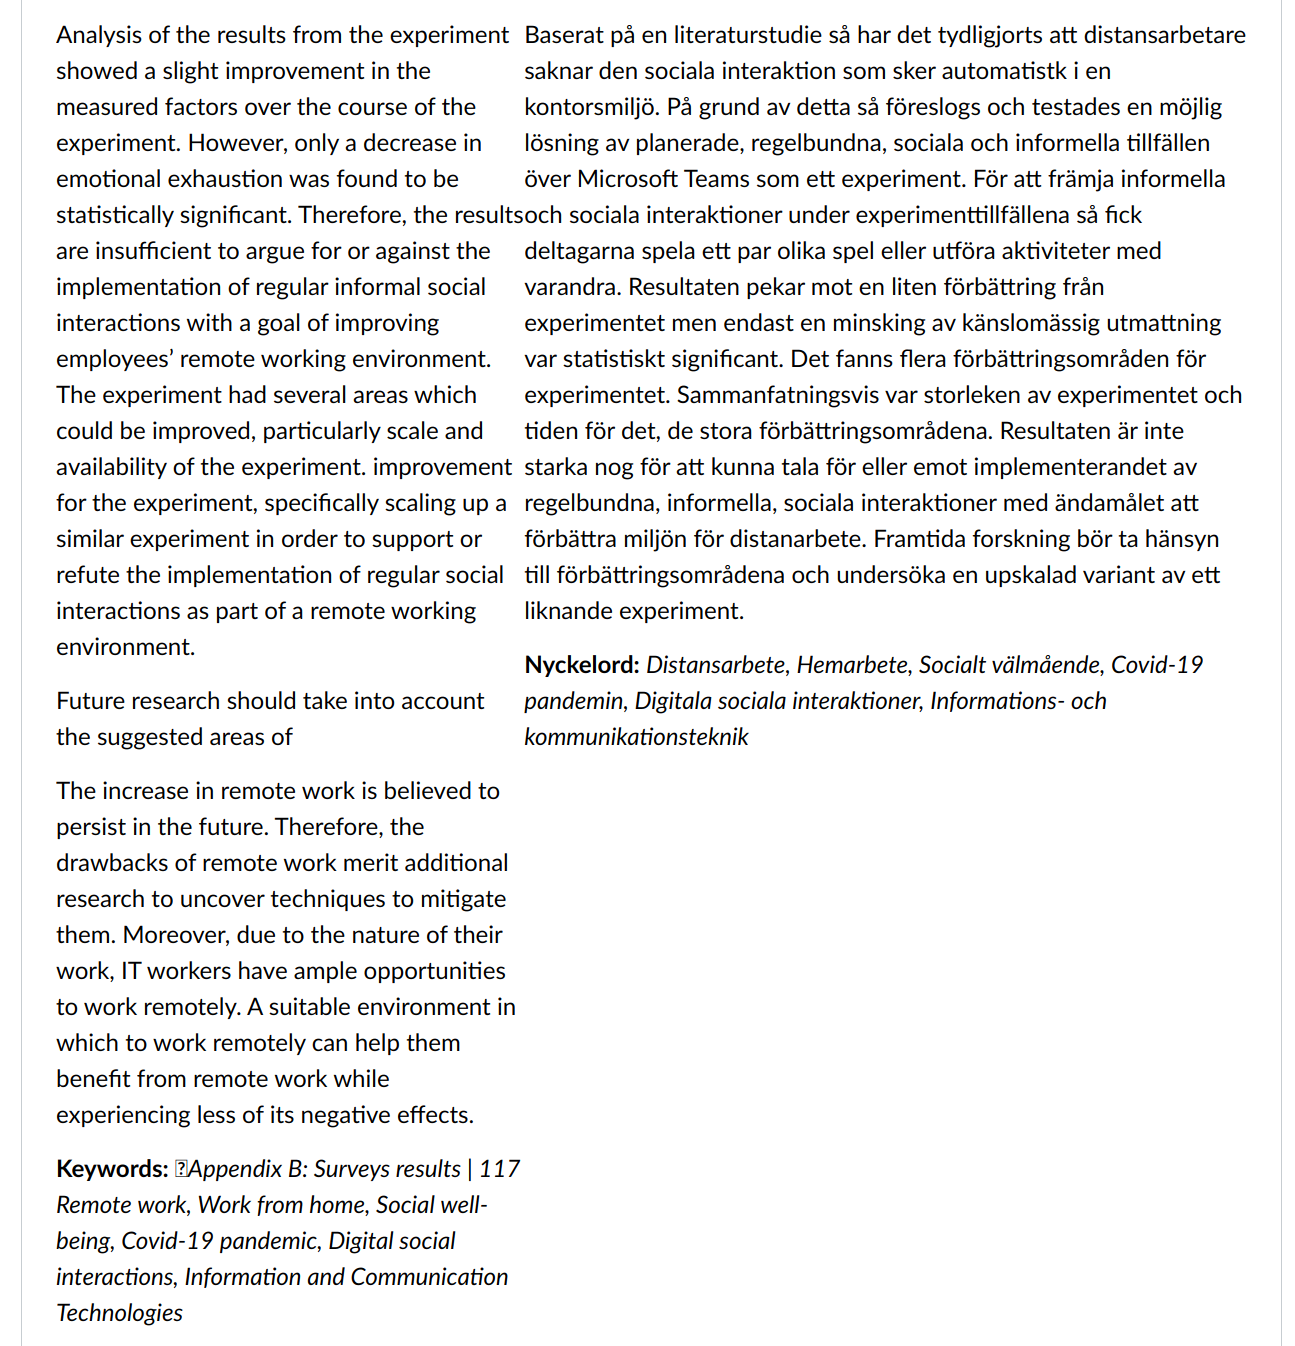
\includegraphics[width=1.2\textwidth]{README_notes/README-examiner-figures/Oscar-2-Screenshot_20210617_140116.png}}
  \end{center}
  \caption{Bottom of the announcement}
  \label{fig:actualAnnouncementBottom}
\end{figure}
\FloatBarrier
	
\begin{figure}[!ht]
  \begin{center}
    \fbox{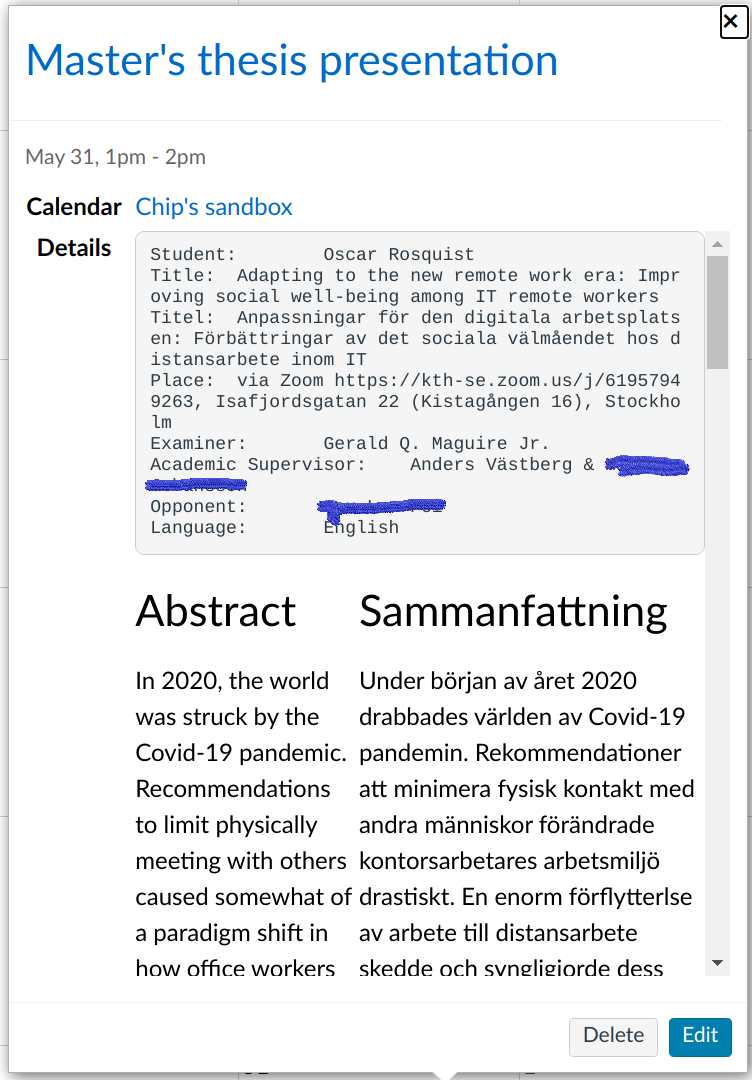
\includegraphics[width=1\textwidth]{README_notes/README-examiner-figures/oscar-course-calendar-Screenshot_20210617_143054.png}}
  \end{center}
  \caption{Opened version in course calendar}
  \label{fig:actualCalendarOpenned}
\end{figure}
\FloatBarrier	

\begin{figure}[!ht]
  \begin{center}
  \begin{subfigure}{0.45\textwidth}
    \fbox{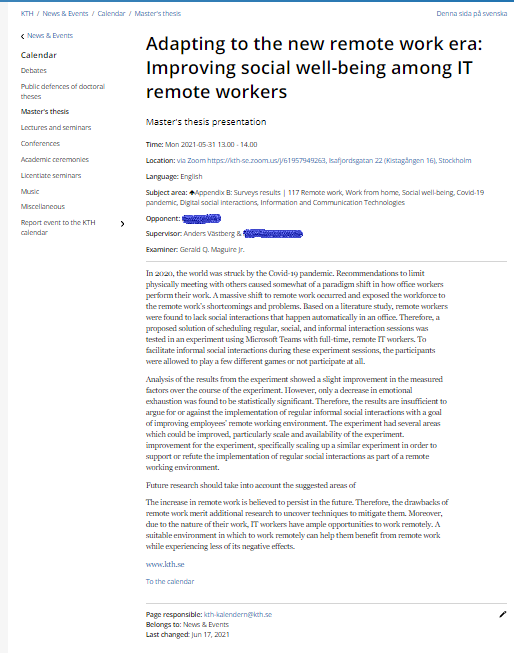
\includegraphics[width=\textwidth]{README_notes/README-examiner-figures/oscar-english-cortina.png}}
    \caption{English}
   \end{subfigure}
   \begin{subfigure}{0.45\textwidth}
    \fbox{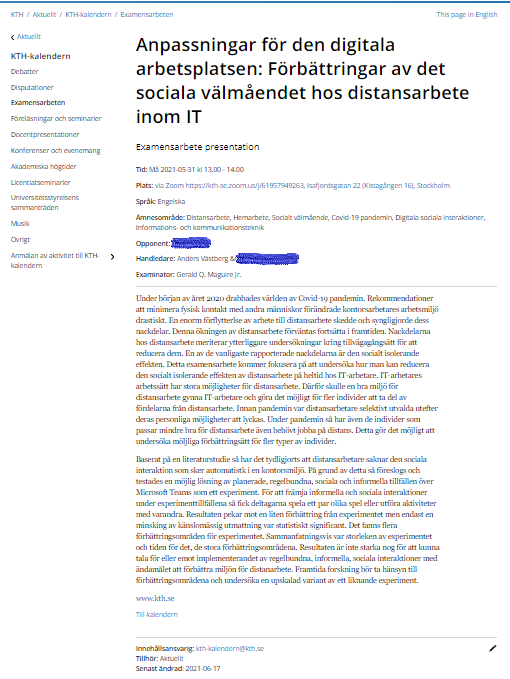
\includegraphics[width=\textwidth]{README_notes/README-examiner-figures/oscar-swedish-cortina.png}}
    \caption{Swedish}
  \end{subfigure}
  \end{center}
  \caption{The English (left) and Swedish (right) in the Cortina calendar}
  \label{fig:actualEnglishAndSwedish}
\end{figure}
\newpage

\Needspace*{4\baselineskip}
\begin{lstlisting}[language={bash}, caption={Commands to extract the JSON and to make the calendar entries and announcements}, label=lst:extractPseudoAndJSONtoCalendar]
./extract_pseudo_JSON-from_PDF.py --pdf oscar.pdf --json oscar.json
./JSON_to_calendar.py -c 11 --config config-test.json --json oscar.json
\end{lstlisting}

\begin{lstlisting}[language={json}, caption={Extracted JSON file oscar.json - edited for appearance here}, label=lst:extractedPseudoAndJSONtoCalendar]
{"Author1": {"Last name": "StudentsLastname", "First name": "StudentsLastname", "Local User Id": "u1000000", "E-mail": "oscarros@kth.se", "organisation": {"L1": "School of XXX"}}, "Degree": {"Educational program": "Degree Programme in XXX"},
"Title": {"Main title": "Adapting to XXX", "Subtitle": "Improving XXX", "Language": "eng"},
"Alternative title": {"Main title": "Anpassningar för XXX", "Subtitle": "Förbättringar av XXX", "Language": "swe"},
"Supervisor1": {"Last name": "Västberg", "First name": "Anders", "Local User Id": "u1ft3a12", "E-mail": "vastberg@kth.se", "organisation": {"L1": "School of XXX", "L2": "StudentsLastname"}},
"Supervisor2": {"Last name": "XXXXX", "First name": "XXXXX", "E-mail": "XXXXXX", "Other organisation": "XXXXX"},
"Examiner1": {"Last name": "ExaminersLastname", "First name": "ExaminersFirstname", "Local User Id": "u1000000", "E-mail": "xxx@kth.se", "organisation": {"L1": "School of XXX", "L2": "DepartmentName"}},
"Cooperation": {"Partner_name": "XXXXX"},
"Other information": {"Year": "2021", "Number of pages": "xvii,115"},
"Opponents": {"Name": "XXXXXX"}, "Presentation": {"Date": "2021-05-31 13:00", "Language": "eng", "Room": "via Zoom https://kth-se.zoom.us/j/61957949263", "Address": "Isafjordsgatan 22 (Kistagången 16)", "City": "Stockholm",
"National Subject Categories": "10201, 10206"}, "Number of lang instances": "2", "abstracts": {"eng": "<p>In 2020, the world was struck by the Covid-19 pandemic. …negative effects.</p>",
"swe": "<p>Under början av året 2020 drabbades världen av Covid-19 pandemin. … ett liknande experiment.</p>"},
"keywords": {"eng": "\n\fAppendix B: Surveys results | 117\n\nRemote work, Work from home, Social well-being, Covid-19 pandemic, Digital social interactions, Information and Communication\nTechnologies ",
"swe": "Distansarbete, Hemarbete, Socialt välmående, Covid-19 pandemin, Digitala sociala interaktioner, Informations- och kommunikationsteknik\n"}}	
\end{lstlisting}


\section{Change in how to enter the abstracts in \LaTeX}
In order to deal with both Babel and Polyglossia and both bibtex and biblatex, I have changed how the abstracts should be entered. Basically the idea is to insert a \textbackslash babelpolyLangStart \{language\_name\}  before the start of the abstract and \textbackslash babelpolyLangStop after the end of the abstract. These commands hide the difference between using Babel or Polyglossia. Additionally, they avoid the problem of the Overleaf GUI being confused about matching beginning and ending statements. \Cref{lst:babel} and \Cref{lst:babelSecondExample} show examples of how to enter an abstract and keywords while \Cref{lst:babelCMDS} shows the definition of the two commands.

Note that both Babel and Polyglossia expand the \textbackslash abstractname into the correct version of the name for an abstract in the current language. Unfortunately, neither package has an equivalent to provide the language specific version of “keywords”, so these have to be provided by the person entering the keywords. For example writing \textbackslash subsection*\{Nyckelord\} to have the Swedish word for keywords set as the subsection heading.

\begin{lstlisting}[language={[LaTeX]TeX}, caption={Example of the revised format for entering an abstract}, label=lst:babel]
\babelpolyLangStart{swedish}
\begin{abstract}
    \markboth{\abstractname}{}
\begin{scontents}[store-env=lang]
swe
\end{scontents}
\begin{scontents}[store-env=abstracts,print-env=true]
Alla avhandlingar vid KTH måste ha ett abstrakt på både engelska och svenska.

Om du skriver din avhandling på svenska ska detta göras först (och placera det som det första abstraktet) - och du bör revidera det vid behov.

If you are writing your thesis in English, you can leave this until the draft version that goes to your opponent for the written opposition. In this way you can provide the English and Swedish abstract/summary information that can be used in the announcement for your oral presentation.

If you are writing your thesis in English, then this section can be a summary targeted at a more general reader. However, if you are writing your thesis in Swedish, then the reverse is true – your abstract should be for your target audience, while an English summary can be written targeted at a more general audience.

This means that the English abstract and \foreignlanguage{swedish}{sammnfattning} 
or Swedish abstract and English summary need not be literal translations of each other.

The abstract in the language used for the thesis should be the first abstract, while the Summary/Sammanfattning in the other language can follow.
\end{scontents}
\subsection*{Nyckelord}
\begin{scontents}[store-env=keywords,print-env=true]
Canvas Lärplattform,Dockerbehållare, prestandajustering
\end{scontents}
\end{abstract}
\babelpolyLangStop{swedish}
\end{lstlisting}
	

\begin{lstlisting}[language={[LaTeX]TeX}, caption={Second example of the revised format for entering an abstract}, label=lst:babelSecondExample]
\generalExpl{Use the relevant language for abstracts for your home university.\\
Note that you may need to augment the set of language used in polyglossia or
babel (see the file kththesis.cls). The following languages include those languages that were used in theses at KTH in 2018-2019, except for one in Chinese.\\
Remove those versions that you do not need.\\
If adding a new language, when specifying the language for the abstract use the three-letter ISO 639-2 Code – specifically the "B" (bibliographic) variant of these codes (note that this is the same language code used in DiVA).
\babelpolyLangStart{french}
\begin{abstract}
    \markboth{\abstractname}{}
\begin{scontents}[store-env=lang]
fre
\end{scontents}
\begin{scontents}[store-env=abstracts,print-env=true]
Résumé en français.
\end{scontents}
\subsection*{Mots clés}
\begin{scontents}[store-env=keywords,print-env=true]
5-6 mots-clés
\end{scontents}
\end{abstract}
\babelpolyLangStop{french}
\cleardoublepage
\end{lstlisting}
\Needspace*{12\baselineskip}
\begin{lstlisting}[language={[LaTeX]TeX}, caption={The two commands used to help enter the language specification}, label=lst:babelCMDS]
\ifxeorlua
    \newcommand{\babelpolyLangStop}[1]{\end{#1}}
\else
    \newcommand{\babelpolyLangStop}[1]{\end{otherlanguage}}
\fi

\ifxeorlua
   \newcommand{\babelpolyLangStart}[1]{\begin{#1}}
\else
    \newcommand{\babelpolyLangStart}[1]{\begin{otherlanguage}{#1}}
\fi
\end{lstlisting}


\section{Adding keywords and PDF metadata}
\label{sec:addingKeywordsAndMetaDataToPDF}
In an effort to add the PDF metadata via the \texttt{hyperref} package, I also decided to add the keywords part of the PDF metadata. However, in order to do this I had to have the keywords \textit{before} the \textbackslash begin\{document\} command in the \LaTeX~file. To do so, I added three new commands to the \texttt{kththesis.cls} file, as shown in \Cref{lst:keywords}. The commands are used in the \texttt{examplethesis.tex} file to set up the keywords in both English and Swedish as well as include a new set of \LaTeX~commands to store the PDF metadata (as shown in \Cref{lst:storingkeywords}) using a file called \texttt{lib/pdf\_related\_includes.tex} (shown in \Cref{lst:informationforPDFfile}). Later the keywords that have been stored are inserted into the \LaTeX~after their respective language abstracts as shown in \Cref{lst:keywordsSection} and \Cref{lst:keywordsSectionSwedish}. The title page of the thesis and the PDF metadata are shown in \Cref{fig:pdfMetadata}. Note that both the English and Swedish version of the keywords are included in the metadata. Finally, the keywords appear (as expected) in the For DiVA data at the end of the PDF file as shown in \Cref{lst:keywordsFromForDIVA}.

Note that \textbackslash makeatletter and \textbackslash makeatother are use to include the character “@” as a letter and then return “@” to being a punctuation code. This use of “@” protects the internal names from being accessed outside of these two commands. More explicitly, \textbackslash EnglishKeywords is a function that takes one argument, the text of the English keywords, and then stores them into “@EnglishKeywords”. Later the text can be retrieved with the command \textbackslash InsertKeywords\{english\} or \textbackslash InsertKeywords\{swedish\}.
\Needspace*{15\baselineskip}
\begin{lstlisting}[language={[LaTeX]TeX}, caption={New commands in kththesis.cls}, label=lst:keywords]
% Keywords
\let\@EnglishKeywords\@empty
\newcommand{\EnglishKeywords}[1]{\def\@EnglishKeywords{#1}}

\let\@SwedishKeywords\@empty
\newcommand{\SwedishKeywords}[1]{\def\@SwedishKeywords{#1}}

\makeatletter
\newcommand{\InsertKeywords}[1]{
    \IfEqCase{#1}{%
    {english}{\@EnglishKeywords}
    {swedish}{\@SwedishKeywords}
  }[\typeout{argument must be english or swedish}]
}
\end{lstlisting}

\Cref{lst:storingkeywords} shows the storing of the keywords using the above commands and the include of the library to set up the PDF metadata.
\Needspace*{10\baselineskip}
\begin{lstlisting}[language={[LaTeX]TeX}, caption={shows the storing of the keywords using the above commands and the include of the library to set up the PDF meta data}, label=lst:storingkeywords]
% Enter the English and Swedish keywords here for use in the PDF meta data _and_ for later use
% following the respective abstract.
% Try to put the words in the same order in both to facilitate matching.
\EnglishKeywords{Canvas Learning Management System, Docker containers, performance tuning}
\SwedishKeywords{Canvas Lärplattform, Dockerbehållare, prestandajustering}

% Put the title, author, and keyword information into the PDF meta information
% This file contains the LaTeX to add information to the PDF file (specifically, author(s), title(s), and keywords
% It uses the hyperref package and should be included before the \begin{document}
%
% I want to acknowledge the inspiration of Karl Voit's template for TU Graz that inspired me to add the PDF document information
% For more information about his template see https://github.com/novoid/LaTeX-KOMA-template
% Note that this template does not use anything from his template other than the names of the information for the PDF meta fields, i.e., mytitle, myauthor, and mykeywords together with the idea of defining the corresponding newcommand to set the relevant hyperref parameters.

\makeatletter
\ifx\@subtitle\@empty
    \newcommand{\mytitle}{\@title}
\else
    \ifinswedish
        \newcommand{\mytitle}{\@title\xspace–\xspace\@subtitle}
    \else
        \newcommand{\mytitle}{\@title: \@subtitle}
    \fi
\fi
\makeatother

% Put the alternative title (and subtitle) into the PDF Subject meta
\makeatletter
\ifx\@altsubtitle\@empty\relax
    \newcommand{\myalttitle}{\@alttitle}
\else
    \ifinswedish
        \newcommand{\myalttitle}{\@alttitle: \@altsubtitle}
    \else
    \newcommand{\myalttitle}{\@alttitle\xspace–\xspace\@altsubtitle}
    \fi
    
\fi
\makeatother
\hypersetup{
     pdfsubject={\myalttitle}        % Subject field
}

\ifinswedish
\XMPLangAlt{en}{pdfsubject={\myalttitle}}
\else
\XMPLangAlt{sv}{pdfsubject={\myalttitle}}
\fi


\ifinswedish
\hypersetup{%
    pdflang={sv},
    pdfmetalang={sv},
    pdftitle={\mytitle}        % Title field
}
\XMPLangAlt{en}{pdftitle={\myalttitle}}
\else
\hypersetup{%
    pdflang={en},
    pdfmetalang={en},
    pdftitle={\mytitle}        % Title field
}
\XMPLangAlt{sv}{pdftitle={\myalttitle}}
\fi

\makeatletter
\ltx@ifpackageloaded{hyperxmp}{
\ifx\@secondAuthorsLastname\@empty
% Note that \hyxmp@comma is used explicitly rather than \xmpcomma
% As the later will simply turn into a comma in this context.
\StrSubstitute{\@authorsLastname}{,}{\hyxmp@comma}[\@authorsLastnameXMP]
    \newcommand{\myauthor}{\xmpquote{\@authorsFirstname\space\@authorsLastnameXMP}} 
\else
% Note that \hyxmp@comma is used explicitly rather than \xmpcomma
% As the later will simply turn into a comma in this context.
\StrSubstitute{\@authorsLastname}{,}{\hyxmp@comma}[\@authorsLastnameXMP]
\StrSubstitute{\@secondAuthorsLastname}{,}{\hyxmp@comma}[\@secondAuthorsLastnameXMP]
    \newcommand{\myauthor}{\xmpquote{\@authorsFirstname\space\@authorsLastnameXMP},
\xmpquote{\@secondAuthorsFirstname\space\@secondAuthorsLastnameXMP}}
\fi
}{
\ifx\@secondAuthorsLastname\@empty
    \newcommand{\myauthor}{\@authorsFirstname\space\@authorsLastname} 
\else
    \newcommand{\myauthor}{\@authorsFirstname\space\@authorsLastname,
\space\@secondAuthorsFirstname\space\@secondAuthorsLastname}
\fi
}% end of ifpackage conditional
\makeatother

\hypersetup{
     pdfauthor={\myauthor}      % Author field
}


\makeatletter
\ifx\@EnglishKeywords\@empty
    \ifx\@SwedishKeywords\@empty
        \newcommand{\mykeywords}{}
    \else
    \newcommand{\mykeywords}{\@SwedishKeywords}
    \fi
\else
    \ifx\@SwedishKeywords\@empty
        \newcommand{\mykeywords}{\@EnglishKeywords}
    \else
        \ifinswedish
            \newcommand{\mykeywords}{\@SwedishKeywords, \@EnglishKeywords}
        \else
            \newcommand{\mykeywords}{\@EnglishKeywords, \@SwedishKeywords}
        \fi
    \fi
\fi
\makeatother

\hypersetup{
     pdfkeywords={\mykeywords}        % Keywords field
}        
% I have _not_ set the following fields:
%    pdfcreator             % Creator field
%    pdfproducer            % Producer field

%% Note that the copyright information is added to the PDF file inside bookinfo{}
%% as until then, the copyright information is unknown.

% Put the alternative title (and subtitle) into the PDF Subject meta
\makeatletter
\ifx\@secondkthid\@empty\relax
    \newcommand{\mykthids}{author: \@kthid}
\else
    \newcommand{\mykthids}{author: \@kthid,\xspace
    secondauthor: \@secondkthid}
\fi
\makeatother

\hypersetup{
     pdfcontactemail={\mykthids}        % Subject field
}

% Add the TRITA number to the metadata
% Get and store information about the series and the number within this series, i.e, TRITA numbers
%"Series": \{
%	"Title of series": "TRITA-ICT-EX"
%	"No. in series": "2019:00"
\makeatletter
\ifinswedish
\hypersetup{
        pdfvolumenum={\@thesisSeries},        % put the series in the volume field
        pdfissuenum={\@thesisSeriesNumber},
        pdfpublisher={Kungliga Tekniska högskolan (KTH)},
        pdfpubtype={report}
}
\else
\hypersetup{
        pdfvolumenum={\@thesisSeries},        % put the series in the volume field
        pdfissuenum={\@thesisSeriesNumber},
        pdfpublisher={KTH Royal Institute of Technology},
        pdfpubtype={report}
}
\fi
\makeatother


% summary
\end{lstlisting}


The \texttt{lib/pdf\_related\_includes.tex} file contains the \LaTeX~to add information
to the PDF file (specifically, author(s), title(s), and keywords. It uses the
\texttt{hyperref} package and should be included before the \textbackslash begin{document}.
I want to acknowledge the inspiration of Karl Voit's template for TU Graz that inspired me to add the PDF document information. For more information about his template see \url{https://github.com/novoid/LaTeX-KOMA-template}
Note that my template does not use anything from his template other than the names of the information for the PDF meta fields, \ie \texttt{mytitle}, \texttt{myauthor}, and \texttt{mykeywords} together with the idea of defining the corresponding \texttt{newcommand} to set the relevant \texttt{hyperref} parameters. A result of both these decisions is that these command names are visible to the rest of the \LaTeX~file. See \Cref{lst:informationforPDFfile} for the code.

In keeping with the Swedish standard (Svenska skrivregler [Språkrådet 1.6.3 och 12.11.5]) a ``mellanslag tankstreck'' with a space before and after, \ie `` – '' is used to separate the title and subtitle when in Swedish this leads to a condition based on whether the document is in Swedish or not in the computation of \texttt{mytitle} and \texttt{myalttitle}.

As a result of adding support for the PDF metadata for copyright notice, the template now uses the \texttt{hyperxmp}. Because of this, if the author's name includes a suffix such as ``, Jr.'' or `` Jr.'', \ie the suffix can be separated with a comma or not as the author prefers to write their name; thus, there was a need to change the processing of \texttt{pdfauthor} information, as \texttt{hyperxmp} treats comma-separated strings in the author or keywords fields as being a list and converts these into a sequence of data in the metadata. This change is shown in \Cref{lst:informationforPDFfile} where the \textbackslash hyxmp@comma macro is used to insert something that is later replaced by a comma but is not treated as a comma when processing the \texttt{pdfauthor} information. The command \textbackslash xmpquote is used to wrap the whole name.
%\clearpage
\begin{lstlisting}[language={[LaTeX]TeX}, caption={lib/pdf\_related\_includes.tex
    (edited for readability and to avoid problems when rendering)}, columns=fullflexible, showstringspaces=false, label=lst:informationforPDFfile]
\makeatletter
\ifx\@subtitle\@empty
    \newcommand{\mytitle}{\@title}
\else
    \ifinswedish
        \newcommand{\mytitle}{\@title\xspace – \xspace\@subtitle}
    \else
        \newcommand{\mytitle}{\@title: \@subtitle}
    \fi
\fi
\makeatother

\makeatletter
\ltx@ifpackageloaded{hyperxmp}{
\ifx\@secondAuthorsLastname\@empty
% Note that \hyxmp@comma is used explicitly rather than \xmpcomma
% As the latter will simply turn into a comma in this context.
\StrSubstitute{\@authorsLastname}{,}{\hyxmp@comma}[\@authorsLastname]
    \newcommand{\myauthor}{\xmpquote{\@authorsFirstname\space\@authorsLastname}} 
\else
% Note that \hyxmp@comma is used explicitly rather than \xmpcomma
% As the latter will simply turn into a comma in this context.
\StrSubstitute{\@authorsLastname}{,}{\hyxmp@comma}[\@authorsLastname]
\StrSubstitute{\@secondAuthorsLastname}{,}{\hyxmp@comma}[\@secondAuthorsLastname]
    \newcommand{\myauthor}{\xmpquote{\@authorsFirstname\space\@authorsLastname},
\xmpquote{\@secondAuthorsFirstname\space\@secondAuthorsLastname}}
\fi
}{
\ifx\@secondAuthorsLastname\@empty
    \newcommand{\myauthor}{\@authorsFirstname\space\@authorsLastname} 
\else
    \newcommand{\myauthor}{\@authorsFirstname\space\@authorsLastname,
\space\@secondAuthorsFirstname\space\@secondAuthorsLastname}
\fi
}% end of ifpackage conditional
\makeatother

\hypersetup{
     pdfauthor={\myauthor}      % Author field
}dfauthor={\myauthor}      % Author field
}

% Put the alternative title (and subtitle) into the PDF Subject meta
\ifx\@altsubtitle\@empty\relax
    \newcommand{\myalttitle}{\@alttitle}
\else
    \ifinswedish
        \newcommand{\myalttitle}{\@alttitle: \@altsubtitle}
    \else
    \newcommand{\myalttitle}{\@alttitle\xspace – \xspace\@altsubtitle}
    \fi
    
\fi

\hypersetup{
     pdfsubject={\myalttitle}        % Subject field
}

\ifx\@EnglishKeywords\@empty
    \ifx\@SwedishKeywords\@empty
        \newcommand{\mykeywords}{}
    \else
    \newcommand{\mykeywords}{\@SwedishKeywords}
    \fi
\else
    \ifx\@SwedishKeywords\@empty
        \newcommand{\mykeywords}{\@EnglishKeywords}
    \else
        \ifinswedish
            \newcommand{\mykeywords}{\@SwedishKeywords, \@EnglishKeywords}
        \else
            \newcommand{\mykeywords}{\@EnglishKeywords, \@SwedishKeywords}
        \fi
    \fi
\fi
\makeatother

\hypersetup{
     pdfkeywords={\mykeywords}        % Keywords field
}        
\end{lstlisting}
\clearpage
\begin{lstlisting}[language={[LaTeX]TeX}, caption={Including the English language keywords below the English abstract}, label=lst:keywordsSection]
\subsection*{Keywords}
\begin{scontents}[store-env=keywords,print-env=true]
% If you set the EnglishKeywords earlier, you can retrieve them with:
% Alternative 1:
%\makeatletter
%\@EnglishKeywords
%\makeatother
%
% Alternative 2:
\InsertKeywords{english}
% If you did not set the EnglishKeywords earlier then simply enter the keywords here:
% Alternative 3:
% comma separate keywords, such as: Canvas Learning Management System, Docker containers, performance tuning
\end{scontents}
\end{lstlisting}

\begin{lstlisting}[language={[LaTeX]TeX}, caption={Including the Swedish language keywords below the Swedish abstract}, label=lst:keywordsSectionSwedish]
\subsection*{Nyckelord}
\begin{scontents}[store-env=keywords,print-env=true]
% SwedishKeywords were set earlier, hence we can use alternative 2
\InsertKeywords{swedish}
\end{scontents}
\end{abstract}
\end{lstlisting}



\begin{figure}[!ht]
  \begin{center}
    \fbox{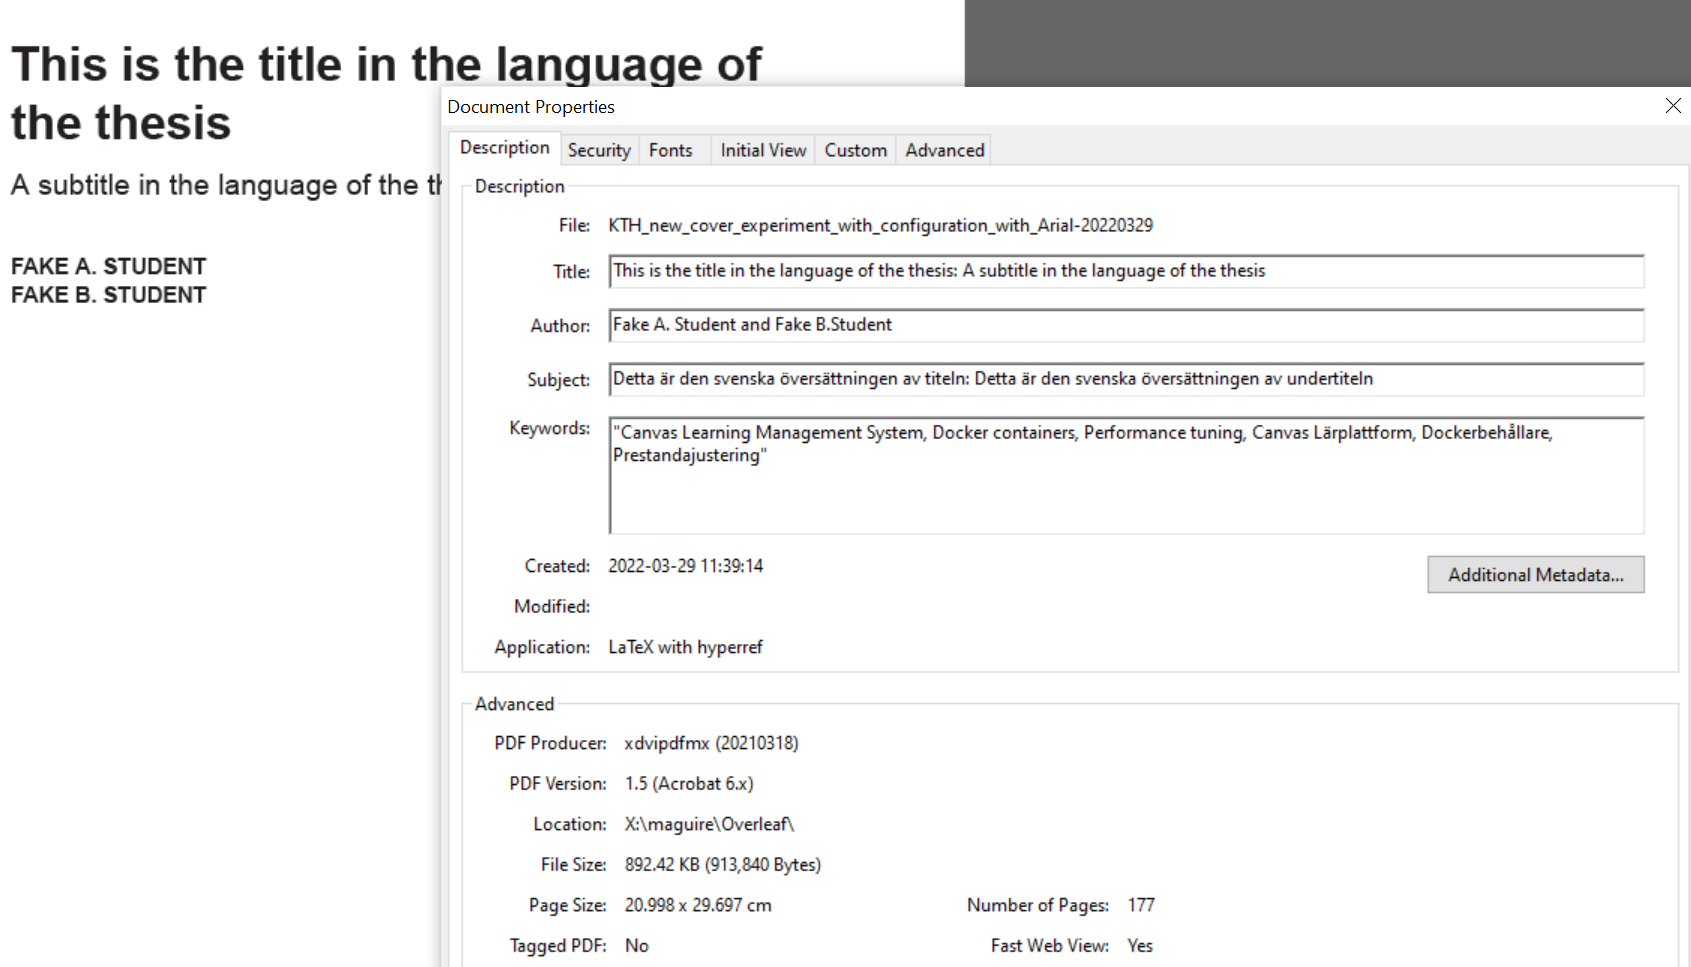
\includegraphics[width=1\textwidth]{README_notes/README-examiner-figures/PDF-file-metadata-Screenshot_20220330_085854.png}}
  \end{center}
  \caption{The title page of the thesis and the PDF metadata}
  \label{fig:pdfMetadata}
\end{figure}
\FloatBarrier	
\Needspace*{7\baselineskip}
\begin{lstlisting}[language={[LaTeX]TeX}, caption={The keywords appear as expected in the For DiVA data at the end of the PDF file}, label=lst:keywordsFromForDIVA]	
”Keywords[eng ]”: €€€€
Canvas Learning Management System, Docker containers, Performance tuning €€€€,

”Keywords[swe ]”: €€€€
Canvas Lärplattform, Dockerbehållare, Prestandajustering €€€€,
\end{lstlisting}

\section{Other variants of the JSON\_to\_calendar.py}
\label{sec:otherVariantsofJSONtoCalendar}
For testing purposes, I also created functionality in \texttt{JSON\_to\_calendar.py} to insert a fixed event (this was my first test) and to take as input a MODS file. The MODS file was created from a DiVA feed of theses presented in 2020 through to the 25\textsuperscript{th} of April. However, one limitation that I found is that other than myself, few people have been entering the date and time for the oral presentation. Unfortunately, since I wanted to test making calendar announcements, I needed data and time!

\Needspace*{2\baselineskip}
\textbf{NB}: I have assumed that each degree project presentation lasts one hour – since the KTH Cortina calendar API needs both a starting and ending time.

These other variants probably should not be kept, but rather the architecture should be similar to that shown in \Cref{fig:severalPossibleInputs}. Additionally, when taking data from other types of sources, one can take advantage of the data that is in a Canvas degree project course room to help when processing of the source data.

\begin{figure}[!ht]
\resizebox{\textwidth}{!}{%
\begin{tikzpicture}
[align=left,node distance=2cm]


\node (latexFile) [tape,tape bend top=none,draw,font=\sffamily] {\LaTeX file};
\node (PDFfile) [tape,tape bend top=none,draw,font=\sffamily, above of=latexFile] {PDF file};
\node (DOCXFile) [tape,tape bend top=none,draw,font=\sffamily, below of=latexFile] {DOCX file};

\node (extractor) [processBox, right=1cm of latexFile] {Extractor};
\node (jsonFile) [tape,tape bend top=none,draw,font=\sffamily, right=0.5cm of extractor] {JSON file};
\node (start) [processBox, right=0.5cm of jsonFile] {JSON\_to\_calendar};
\node (MODSFile) [tape,tape bend top=none,draw,font=\sffamily, above of=jsonFile] {MODS file};

\node (calendarEvent) [destinationBox, right=1cm of start] {Canvas calendar event};
\node (announcement) [destinationBox,  above of =calendarEvent] {Canvas announcement};
\node (cortinaCalendarEvent) [destinationBox,  right=0.5cm of start, below of=calendarEvent] {KTH Cortina calendar event};
\draw [arrow] (latexFile) --  (extractor.west);
\draw [arrow] (PDFfile) --  (extractor.west);
\draw [arrow] (DOCXFile) --  (extractor.west);
\draw [arrow] (extractor) --  (jsonFile.west);
\draw [arrow] (jsonFile) --  (start.west);
\draw [arrow] (start.east) --  (announcement.west);
\draw [arrow] (start.east) -- (calendarEvent);
\draw [arrow] (start.east) -- (cortinaCalendarEvent.west);
\draw [arrow, dashed] (MODSFile) --  node[right] {only for testing} (start.west);
\end{tikzpicture}
}
\caption{Several possible inputs to JSON\_to\_calendar.py  and its outputs}
  \label{fig:severalPossibleInputs}
\end{figure}




\section{JSON to MODS file}
\label{sec:JSONtoMODSfile}
In keeping with the idea of using the JSON file to drive other applications, the program JSON\_to\_MODS.py to creates a MODS file using the information from the arguments and a JSON file.
The program is patterned after the \texttt{JSON\_to\_calendar} and \texttt{JSON\_to\_cover} programs. The program outputs a MODS file called: \texttt{modsXML.xml}. The program is run as shown in \Cref{lst:jsonToMods}.
\Needspace*{5\baselineskip}
\begin{lstlisting}[language={bash}, caption={Example of using JSON\_to\_MODS.py}, label=lst:jsonToMods]
./JSON_to_MODS.py -c 11   --json test12.json --trita "TRITA-EECS-EX-2021:219" --testing
\end{lstlisting}


Note that currently the Canvas course information is not used. Note also that the “—testing” flag forces the report series to be  "TRITA-ICT-EX" overriding the actual series in in the input version of the DiVA data.

If acronyms are used in the abstracts, you can also add the “- -acronyms acronyms.tex” argument to the command line and the program will process the acronyms.

As noted above, you will get a file named \texttt{modsXML.xml} that you can manually import into DiVA. This process is shown in \Cref{sec:importingMODSfiletoDiVA}. I seem to be able to import these files into the test instance of DiVA:	\url{https://kth.test.diva-portal.org/dream/import/importList.jsf}. Another side-effect of the testing flag is to use the test instance of DiVA. \textbf{NB}: The organization units are different between the production and test version of DiVA. When run without the testing flag set, the MODS file can be imported into the production version of DiVA.

This program has been extended to be able to take the TRITA number information from the MODS file.


\subsection{Example of JSON to MODS}
The process of importing the MODS data into DiVA begins with the extracted JSON file (note that I have changed some of the formatting of the pseudo JSON information and added the export of the program code). An example of the JSON information is shown in \Cref{lst:test12.json}. The resulting MODS file is shown in \Cref{lst:test12.mods}.

\begin{lstlisting}[language={json}, caption={test12.json (manually reformatted)}, label=lst:test12.json]
{"Author1": {"Last name": "Student", "First name": "Fake A.", "Local User Id": "u100001", "E-mail": "a@kth.se", "organisation": {"L1": "School of XXX"}}, 
"Author2": {"Last name": "Student", "First name": "Fake B.", "Local User Id": "u100002", "E-mail": "b@kth.se", "organisation": {"L1": "School of XXX"}}, 
"Degree": {"Educational program": "Bachelor’s Programme in XXX", "programcode": "TCOMK", "Level": "1", "Course code": "XX100X", "Credits": "15.0", "Exam": "Bachelors degree", "subjectArea": "subject area"},
"Title": {"Main title": "This is the title in the language of the thesis", "Subtitle": "An subtitle in the language of the thesis", "Language": "eng"},
"Alternative title": {"Main title": "Detta är den svenska översättningen av titeln", "Subtitle": "Detta är den svenska översättningen av undertiteln", "Language": "swe"},
"Supervisor1": {"Last name": "Supervisor", "First name": "A. Busy", "Local User Id": "u100003", "E-mail": "sa@kth.se", "organisation": {"L1": "School of XXX", "L2": "DepartmentName"}},
"Supervisor2": {"Last name": "Supervisor", "First name": "Another Busy", "Local User Id": "u100003", "E-mail": "sb@kth.se", "organisation": {"L1": "School of XXX", "L2": "DepartmentName"}}, 
"Supervisor3": {"Last name": "Supervisor", "First name": "Third Busy", "E-mail": "sc@tu.va", "Other organisation": "Timbuktu University, Department of Pseudoscience"},
"Examiner1": {"Last name": "ExaminersLastname", "First name": "ExaminersFirstname", "Local User Id": "u1000000", "E-mail": "xxx@kth.se", "organisation": {"L1": "School of XXX", "L2": "DepartmentName"}},
"Cooperation": {"Partner_name": "Företaget AB"}, "National Subject Categories": "10201, 10206", "Other information": {"Year": "2021", "Number of pages": "xxxiii,35"}, "Opponents": {"Name": "A. B. Normal & A. X. E. Normalè"}, "Presentation": {"Date": "2021-03-15 13:00", "Language": "eng", "Room": "via Zoom https://kth-se.zoom.us/j/ddddddddddd", "Address": "Isafjordsgatan 22 (Kistagången 16)", "City": "Stockholm"},
"Number of lang instances": "10", "abstracts": {"eng": "<p>All theses at KTH are <bold>required</bold> to have an abstract in both <i>English</i> and <i>Swedish</i>.</p><p>Exchange students many want to include one or more abstracts in the language(s) used in their home institutions to avoid the need to write another thesis when returning to their home institution.</p><p>Keep in mind that most of your potential readers are only going to read your <tt>title</tt> and <tt>abstract</tt>. This is why it is important that the abstract give them enough information that they can decide is this document relevant to them or not. Otherwise the likely default choice is to ignore the rest of your document.</p><p>A abstract should stand on its own, i.e., no citations, cross references to the body of the document, acronyms must be spelled out, … .</p><p>Write this early and revise as necessary. This will help keep you focused on what you are trying to do.</p><p>Write an abstract with the following components: </p><ul><li> What is the topic area? (optional) Introduces the subject area for the project. </li><li> Short problem statement </li><li> Why was this problem worth a Bachelor’s/’Masters thesis project? (i.e., why is the problem both significant and of a suitable degree of difficulty for a Bachelor’s/’Masters thesis project? Why has no one else solved it yet?) </li><li> How did you solve the problem? What was your method/insight? </li><li> Results/Conclusions/Consequences/Impact: What are your key results/conclusions? What will others do based upon your results? What can be done now that you have finished - that could not be done before your thesis project was completed?</li></ul><p>announcement of the oral presentation and for entering data into DiVA</p><p>\\pi \\cdot r$ or \\[ \\int_{a}^{b} x^2 \\,dx \\]</p><p></p><p> A<sup>*</sup>, A<sup>&reg;</sup>, and A&trade;.</p><p> first chemical formula can be handled, while the second will require hand editing</p>",
"swe": "<p>Alla avhandlingar vid KTH <bold>måste ha</bold> ett abstrakt på både <i>engelska</i> och <i>svenska</i>.</p><p>Om du skriver din avhandling på svenska ska detta göras först (och placera det som det första abstraktet) - och du bör revidera det vid behov.</p><p>If you are writing your thesis in English, you can leave this until the draft version that goes to your opponent for the written opposition. In this way you can provide the English and Swedish abstract/summary information that can be used in the announcement for your oral presentation.</p><p>If you are writing your thesis in English, then this section can be a summary targeted at a more general reader. However, if you are writing your thesis in Swedish, then the reverse is true – your abstract should be for your target audience, while an English summary can be written targeted at a more general audience.</p><p>This means that the English abstract and Swedish sammnfattning or Swedish abstract and English summary need not be literal translations of each other.</p><p>The abstract in the language used for the thesis should be the first abstract, while the Summary/Sammanfattning in the other language can follow.</p>",
"fre": "<p>Résumé en français.</p>", "spa": "<p>Résumé en espagnol.</p>", "ita": "<p>Sommario in italiano.</p>",
"nor": "<p>Sammendrag på norsk.</p>", "ger": "", "dan": "<p>Abstrakt på dansk.</p>",
"dut": "<p>Zusammenfassung in Deutsch.</p><p>Samenvatting in het Nederlands.</p><p>Eesti keeles kokkuvõte.</p>", "est": ""},
"keywords": {"eng": "Canvas Learning Management System, Docker containers, Performance tuning ",
"swe": "Canvas Lärplattform, Dockerbehållare, Prestandajustering\nNyckelord som beskriver innehållet i uppsatsrapporten\n",
"fre": "5-6 mots-clés ", "spa": "5-6 Palabras claves ", "ita": "5-6 parole chiave ",
"nor": "5-6 nøkkelord ", "ger": "5-6 Schlüsselwörter ", "dan": "5-6 Søgeord ",
"dut": "5-6 trefwoorden ", "est": "5-6 Märksõnad "}}
\end{lstlisting}

\clearpage

\begin{lstlisting}[language={XML}, caption={test12.mods (reformatted in EMACS using XML mode)}, label=lst:test12.mods]
<modsCollection xmlns="http://www.loc.gov/mods/v3" xmlns:xsi="http://www.w3.org/2001/XMLSchema-instance" xsi:schemaLocation="http://www.loc.gov/mods/v3 http://www.loc.gov/standards/mods/v3/mods-3-2.xsd">
  <mods xmlns="http://www.loc.gov/mods/v3" xmlns:xsi="http://www.w3.org/2001/XMLSchema-instance" xmlns:xlink="http://www.w3.org/1999/xlink" version="3.2" xsi:schemaLocation="http://www.loc.gov/mods/v3 http://www.loc.gov/standards/mods/v3/mods-3-2.xsd">
    <genre authority="diva" type="publicationTypeCode">studentThesis
    </genre>
    <genre authority="diva" type="publicationType" lang="swe">Studentuppsats (Examensarbete)
    </genre>
    <genre authority="diva" type="publicationType" lang="eng">Student thesis
    </genre>
    <genre authority="diva" type="publicationType" lang="nor">Oppgave
    </genre>
    <name type="personal" authority="kth" xlink:href="u100001">
      <namePart type="family">Student
      </namePart>
      <namePart type="given">Fake A.
      </namePart>
      <description>email=a@kth.se
      </description>
      <role>
	<roleTerm type="code" authority="marcrelator">aut
	</roleTerm>
      </role>
    </name>
    <name type="personal" authority="kth" xlink:href="u100002">
      <namePart type="family">Student
      </namePart>
      <namePart type="given">Fake B.
      </namePart>
      <description>email=b@kth.se
      </description>
      <role>
	<roleTerm type="code" authority="marcrelator">aut
	</roleTerm>
      </role>
    </name>
    <name type="personal" authority="kth" xlink:href="u1d13i2c">
      <namePart type="family">Maguire Jr.
      </namePart>
      <namePart type="given">Gerald Q.
      </namePart>
      <description>email=maguire@kth.se
      </description>
      <affiliation>KTH, School of XXX, DepartmentName
      </affiliation>
      <role>
	<roleTerm type="code" authority="marcrelator">mon
	</roleTerm>
      </role>
    </name>
    <name type="personal" authority="kth" xlink:href="u100003">
      <namePart type="family">Supervisor
      </namePart>
      <namePart type="given">A. Busy
      </namePart>
      <affiliation>School of School of XXX, DepartmentName
      </affiliation>
      <description>email=sa@kth.se
      </description>
      <role>
	<roleTerm type="code" authority="marcrelator">ths
	</roleTerm>
      </role>
    </name>
    <name type="personal" authority="kth" xlink:href="u100003">
      <namePart type="family">Supervisor
      </namePart>
      <namePart type="given">Another Busy
      </namePart>
      <affiliation>School of School of XXX, DepartmentName
      </affiliation>
      <description>email=sb@kth.se
      </description>
      <role>
	<roleTerm type="code" authority="marcrelator">ths
	</roleTerm>
      </role>
    </name>
    <name type="personal">
      <namePart type="family">Supervisor
      </namePart>
      <namePart type="given">Third Busy
      </namePart>
      <affiliation>Timbuktu University, Department of Pseudoscience
      </affiliation>
      <description>email=sc@tu.va
      </description>
      <role>
	<roleTerm type="code" authority="marcrelator">ths
	</roleTerm>
      </role>
    </name>
    <name>
      <namePart>KTH
      </namePart>
      <namePart> School of XXX
      </namePart>
      <namePart> DepartmentName
      </namePart>
      <role>
	<roleTerm type="code" authority="marcrelator">pbl
	</roleTerm>
      </role>
    </name>
    <titleInfo  lang="eng">
      <title>This is the title in the language of the thesis
      </title>
      <subTitle>An subtitle in the language of the thesis
      </subTitle>
    </titleInfo >
    <titleInfo  lang="swe" type="alternative">
      <title>Detta är den svenska översättningen av titeln
      </title>
      <subTitle>Detta är den svenska översättningen av undertiteln
      </subTitle>
    </titleInfo >
    <subject  lang="eng">
      <topic>Canvas Learning Management System
      </topic>
      <topic>Docker containers
      </topic>
      <topic>Performance tuning
      </topic>
    </subject >
    <subject  lang="swe">
      <topic>Canvas Lärplattform
      </topic>
      <topic>Dockerbehållare
      </topic>
      <topic>Prestandajustering Nyckelord som beskriver innehållet i uppsatsrapporten
      </topic>
    </subject >
    <subject  lang="fre">
      <topic>5-6 mots-clés
      </topic>
    </subject >
    <subject  lang="spa">
      <topic>5-6 Palabras claves
      </topic>
    </subject >
    <subject  lang="ita">
      <topic>5-6 parole chiave
      </topic>
    </subject >
    <subject  lang="nor">
      <topic>5-6 nøkkelord
      </topic>
    </subject >
    <subject  lang="ger">
      <topic>5-6 Schlüsselwörter
      </topic>
    </subject >
    <subject  lang="dan">
      <topic>5-6 Søgeord
      </topic>
    </subject >
    <subject  lang="dut">
      <topic>5-6 trefwoorden
      </topic>
    </subject >
    <subject  lang="est">
      <topic>5-6 Märksõnad
      </topic>
    </subject >
    <abstract  lang="eng">&lt;p&gt;All theses at KTH are &lt;bold&gt;required&lt;/bold&gt; to have an abstract in both &lt;i&gt;English&lt;/i&gt; and &lt;i&gt;Swedish&lt;/i&gt;.&lt;/p&gt;&lt;p&gt;Exchange students many want to include one or more abstracts in the language(s) used in their home institutions to avoid the need to write another thesis when returning to their home institution.&lt;/p&gt;&lt;p&gt;Keep in mind that most of your potential readers are only going to read your &lt;tt&gt;title&lt;/tt&gt; and &lt;tt&gt;abstract&lt;/tt&gt;. This is why it is important that the abstract give them enough information that they can decide is this document relevant to them or not. Otherwise the likely default choice is to ignore the rest of your document.&lt;/p&gt;&lt;p&gt;A abstract should stand on its own, i.e., no citations, cross references to the body of the document, acronyms must be spelled out, … .&lt;/p&gt;&lt;p&gt;Write this early and revise as necessary. This will help keep you focused on what you are trying to do.&lt;/p&gt;&lt;p&gt;Write an abstract with the following components: &lt;/p&gt;&lt;ul&gt;&lt;li&gt; What is the topic area? (optional) Introduces the subject area for the project. &lt;/li&gt;&lt;li&gt; Short problem statement &lt;/li&gt;&lt;li&gt; Why was this problem worth a Bachelor’s/’Masters thesis project? (i.e., why is the problem both significant and of a suitable degree of difficulty for a Bachelor’s/’Masters thesis project? Why has no one else solved it yet?) &lt;/li&gt;&lt;li&gt; How did you solve the problem? What was your method/insight? &lt;/li&gt;&lt;li&gt; Results/Conclusions/Consequences/Impact: What are your key results/conclusions? What will others do based upon your results? What can be done now that you have finished - that could not be done before your thesis project was completed?&lt;/li&gt;&lt;/ul&gt;&lt;p&gt;announcement of the oral presentation and for entering data into DiVA&lt;/p&gt;&lt;p&gt;\pi \cdot r$ or &lt;span class='math-tex'&gt;\[ \int_{a}^{b} x^2 \,dx \]&lt;/span&gt;&lt;/p&gt;&lt;p&gt;&lt;/p&gt;&lt;p&gt; A&lt;sup&gt;*&lt;/sup&gt;, A&lt;sup&gt;&amp;reg;&lt;/sup&gt;, and A&amp;trade;.&lt;/p&gt;&lt;p&gt; first chemical formula can be handled, while the second will require hand editing&lt;/p&gt;
    </abstract >
    <abstract  lang="swe">&lt;p&gt;Alla avhandlingar vid KTH &lt;bold&gt;måste ha&lt;/bold&gt; ett abstrakt på både &lt;i&gt;engelska&lt;/i&gt; och &lt;i&gt;svenska&lt;/i&gt;.&lt;/p&gt;&lt;p&gt;Om du skriver din avhandling på svenska ska detta göras först (och placera det som det första abstraktet) - och du bör revidera det vid behov.&lt;/p&gt;&lt;p&gt;If you are writing your thesis in English, you can leave this until the draft version that goes to your opponent for the written opposition. In this way you can provide the English and Swedish abstract/summary information that can be used in the announcement for your oral presentation.&lt;/p&gt;&lt;p&gt;If you are writing your thesis in English, then this section can be a summary targeted at a more general reader. However, if you are writing your thesis in Swedish, then the reverse is true – your abstract should be for your target audience, while an English summary can be written targeted at a more general audience.&lt;/p&gt;&lt;p&gt;This means that the English abstract and Swedish sammnfattning or Swedish abstract and English summary need not be literal translations of each other.&lt;/p&gt;&lt;p&gt;The abstract in the language used for the thesis should be the first abstract, while the Summary/Sammanfattning in the other language can follow.&lt;/p&gt;
    </abstract >
    <abstract  lang="fre">&lt;p&gt;Résumé en français.&lt;/p&gt;
    </abstract >
    <abstract  lang="spa">&lt;p&gt;Résumé en espagnol.&lt;/p&gt;
    </abstract >
    <abstract  lang="ita">&lt;p&gt;Sommario in italiano.&lt;/p&gt;
    </abstract >
    <abstract  lang="nor">&lt;p&gt;Sammendrag på norsk.&lt;/p&gt;
    </abstract >
    <abstract  lang="ger" />
    <abstract  lang="dan">&lt;p&gt;Abstrakt på dansk.&lt;/p&gt;
    </abstract >
    <abstract  lang="dut">&lt;p&gt;Zusammenfassung in Deutsch.&lt;/p&gt;&lt;p&gt;Samenvatting in het Nederlands.&lt;/p&gt;&lt;p&gt;Eesti keeles kokkuvõte.&lt;/p&gt;
    </abstract >
    <abstract  lang="est" />
    <physicalDescription>
      <form authority="marcform">electronic
      </form>
      <extent>xxxiii,35
      </extent>
    </physicalDescription>
    <originInfo>
      <place>
	<placeTerm>Stockholm
	</placeTerm>
      </place>
      <publisher>KTH Royal Institute of Technology
      </publisher>
      <dateIssued>2021
      </dateIssued>
      <dateOther type="defence">2021-03-15T13:00:00
      </dateOther>
    </originInfo>
    <typeOfResource>text
    </typeOfResource>
    <relatedItem  type="series">
      <titleInfo>
	<title>TRITA-ICT-EX
	</title>
	<identifier type="local">5952
	</identifier>
	<identifier type="issue number">2021:219
	</identifier>
      </titleInfo>
    </relatedItem >
    <note lang="swe" type="level">Självständigt arbete på grundnivå (kandidatexamen)
    </note>
    <note lang="eng" type="degree">Bachelors degree
    </note>
    <note lang="swe" type="universityCredits">10 poäng / 15 hp
    </note>
    <subject lang="swe" xlink:href="10329">
      <topic>Informations- och kommunikationsteknik
      </topic>
      <genre>Subject/course
      </genre>
    </subject>
    <subject lang="eng" xlink:href="10329">
      <topic>Information and Communication Technology
      </topic>
      <genre>Subject/course
      </genre>
    </subject>
    <subject lang="swe" xlink:href="9925">
      <topic>Teknologie kandidatexamen - Informations- och kommunikationsteknik
      </topic>
      <genre>Educational program
      </genre>
    </subject>
    <subject lang="eng" xlink:href="9925">
      <topic>Bachelor of Science - Information and Communication Technology
      </topic>
      <genre>Educational program
      </genre>
    </subject>
    <language objectPart="defence">
      <languageTerm type="code" authority="iso639-2b">eng
      </languageTerm>
    </language>
    <note type="venue">via Zoom https://kth-se.zoom.us/j/ddddddddddd,Isafjordsgatan 22 (Kistagången 16),Stockholm
    </note>
    <note type="cooperation">Företaget AB
    </note>
    <subject lang="eng" authority="hsv" xlink:href="10201">
      <topic>Natural Sciences
      </topic>
      <topic>Computer and Information Sciences
      </topic>
      <topic>Computer Sciences
      </topic>
    </subject>
    <subject lang="swe" authority="hsv" xlink:href="10201">
      <topic>Naturvetenskap
      </topic>
      <topic>Data- och informationsvetenskap
      </topic>
      <topic>Datavetenskap (datalogi)
      </topic>
    </subject>
    <subject lang="eng" authority="hsv" xlink:href="10206">
      <topic>Natural Sciences
      </topic>
      <topic>Computer and Information Sciences
      </topic>
      <topic>Computer Engineering
      </topic>
    </subject>
    <subject lang="swe" authority="hsv" xlink:href="10206">
      <topic>Naturvetenskap
      </topic>
      <topic>Data- och informationsvetenskap
      </topic>
      <topic>Datorteknik
      </topic>
    </subject>
  </mods>
</modsCollection>
\end{lstlisting}
	
\subsection{Importing MODS file to DiVA}
\label{sec:importingMODSfiletoDiVA}

\Cref{fig:divaImport1} to \Cref{fig:divaImport4} show the process of importing the MODS file into DiVA. Note that it skips the first user interface form (as this differs between users).

\begin{figure}[!ht]
  \begin{center}
    \fbox{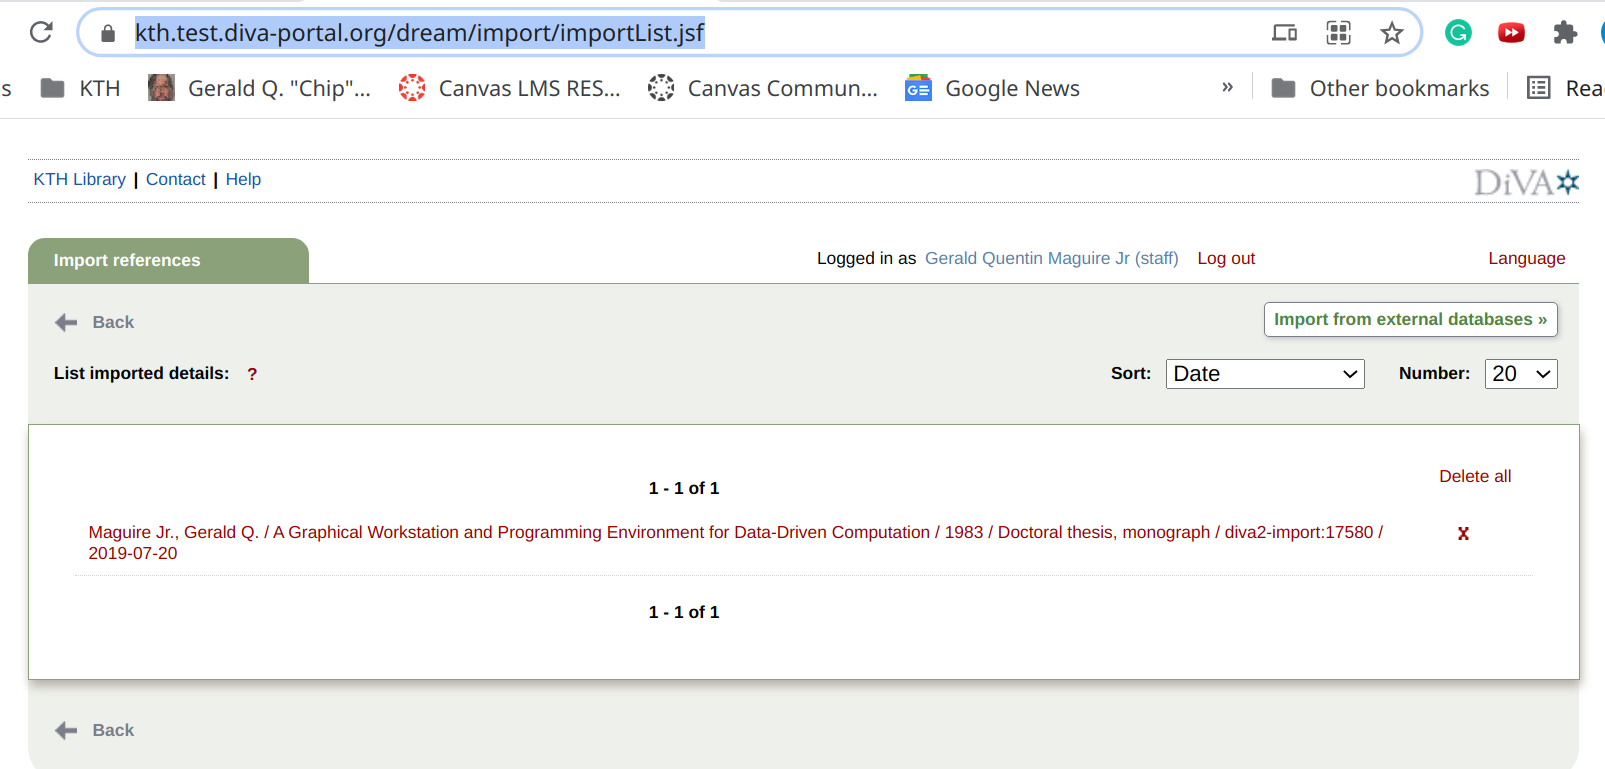
\includegraphics[width=1\textwidth]{README_notes/README-examiner-figures/import-1-Screenshot_20210626_234259.png}}
  \end{center}
  \caption[The import process – step 1]{The import process – step 1 – click on the “Import from external database” button on the upper right corner}
  \label{fig:divaImport1}
\end{figure}
\FloatBarrier

\begin{figure}[!ht]
  \begin{center}
    \fbox{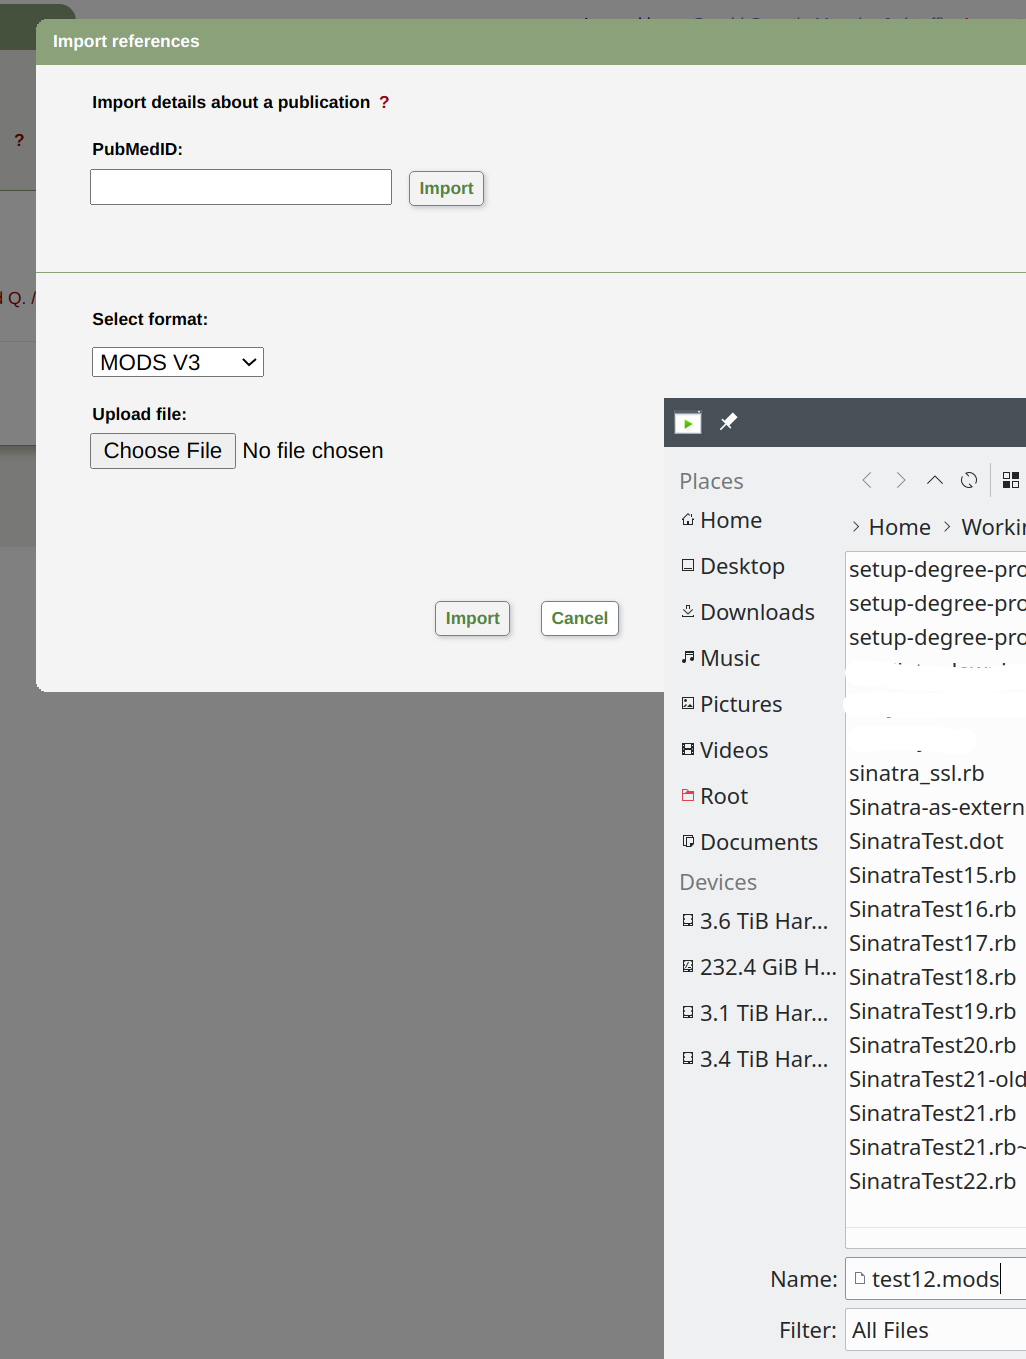
\includegraphics[width=1\textwidth]{README_notes/README-examiner-figures/import-2-Screenshot_20210626_234414.png}}
  \end{center}
  \caption[The import process – step 2]{The import process – step 2 – choose the MODV3 format and select a file to import}
  \label{fig:divaImport2}
\end{figure}
\FloatBarrier

\begin{figure}[!ht]
  \begin{center}
    \fbox{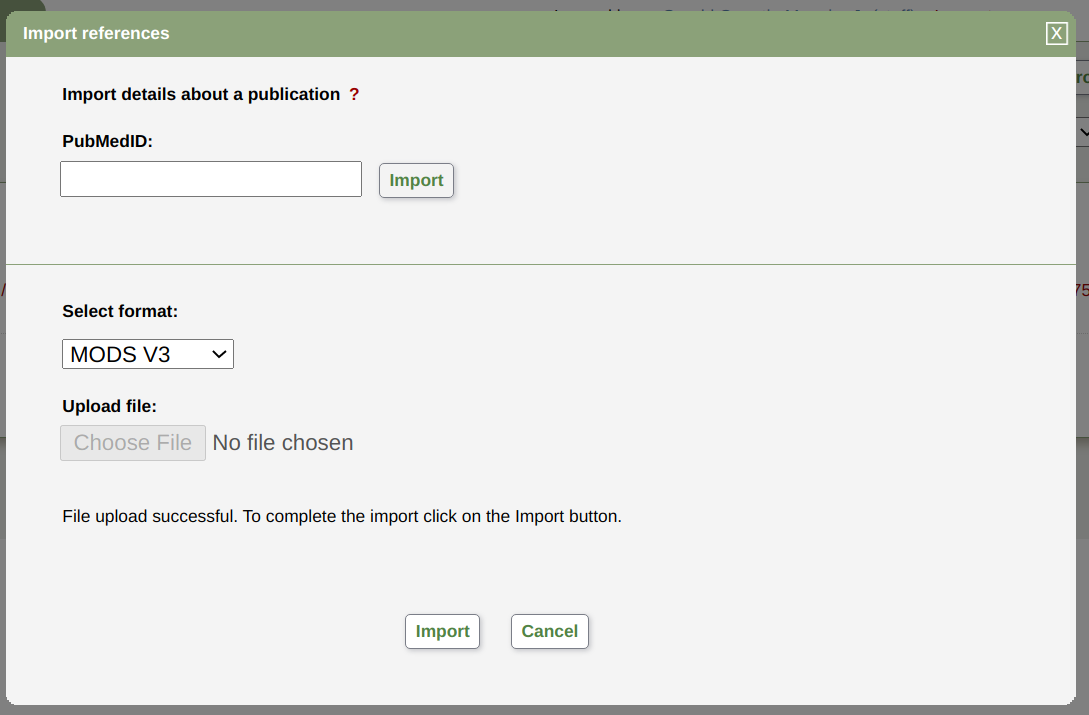
\includegraphics[width=1\textwidth]{README_notes/README-examiner-figures/import-3-Screenshot_20210626_234447.png}}
  \end{center}
  \caption[The import process – step 3]{The import process – step 3 – after clicking “Import” – it says that the file was successfully uploaded
Click on “Import” again to load the file. The MODS files is loaded and shown in \Cref{fig:divaImport4}.}
  \label{fig:divaImport3}
\end{figure}
\FloatBarrier

\begin{figure}[!ht]
  \begin{center}
    \fbox{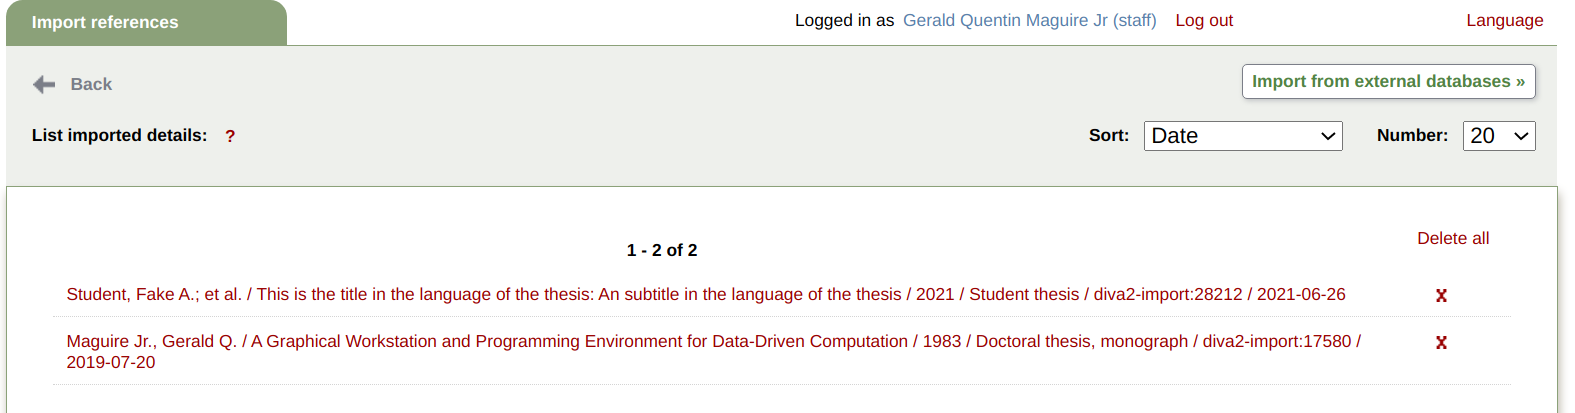
\includegraphics[width=1\textwidth]{README_notes/README-examiner-figures/import-4-Screenshot_20210626_234519.png}}
  \end{center}
  \caption[The import process – step 4]{The import process – step 4 – after clicking “Import” once more – you can see the file has been added to the list of imported files The imported document is shown in \Cref{fig:divaImport5} to \Cref{fig:divaImport12}.}
  \label{fig:divaImport4}
\end{figure}
\FloatBarrier

\begin{figure}[!ht]
  \begin{center}
    \fbox{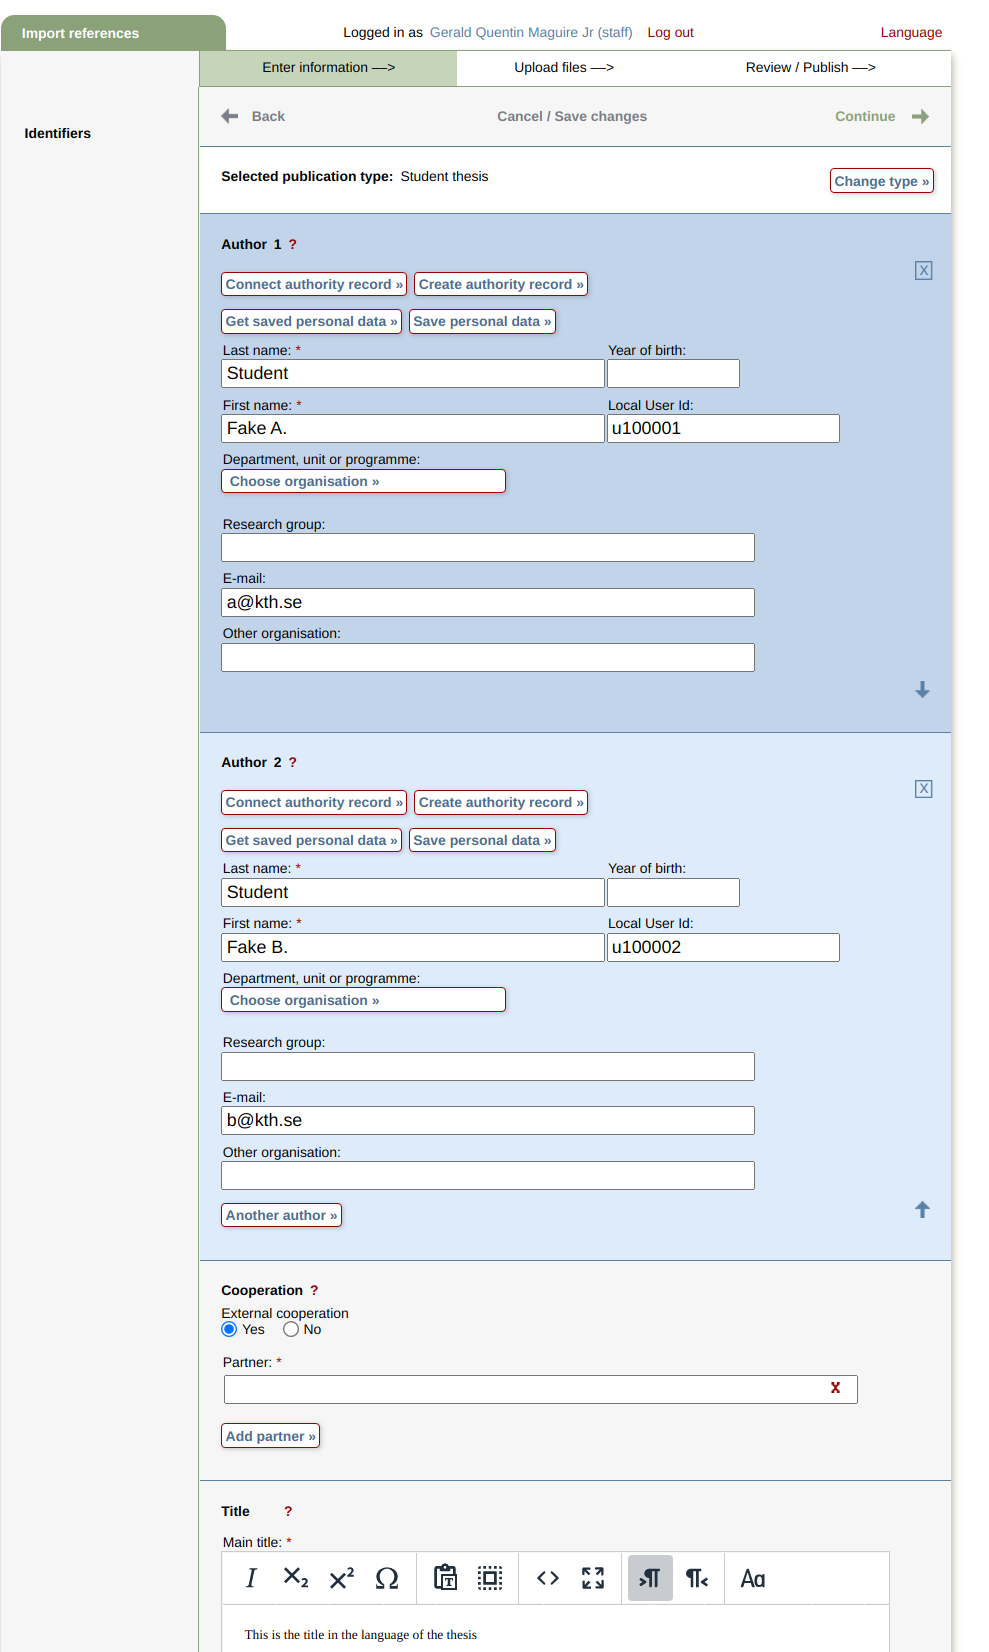
\includegraphics[width=0.8\textwidth]{README_notes/README-examiner-figures/import-a-Screenshot_20210626_234606.png}}
  \end{center}
  \caption[Imported document (part 1)]{Imported document (part 1)}
  \label{fig:divaImport5}
\end{figure}
\FloatBarrier

\begin{figure}[!ht]
  \begin{center}
    \fbox{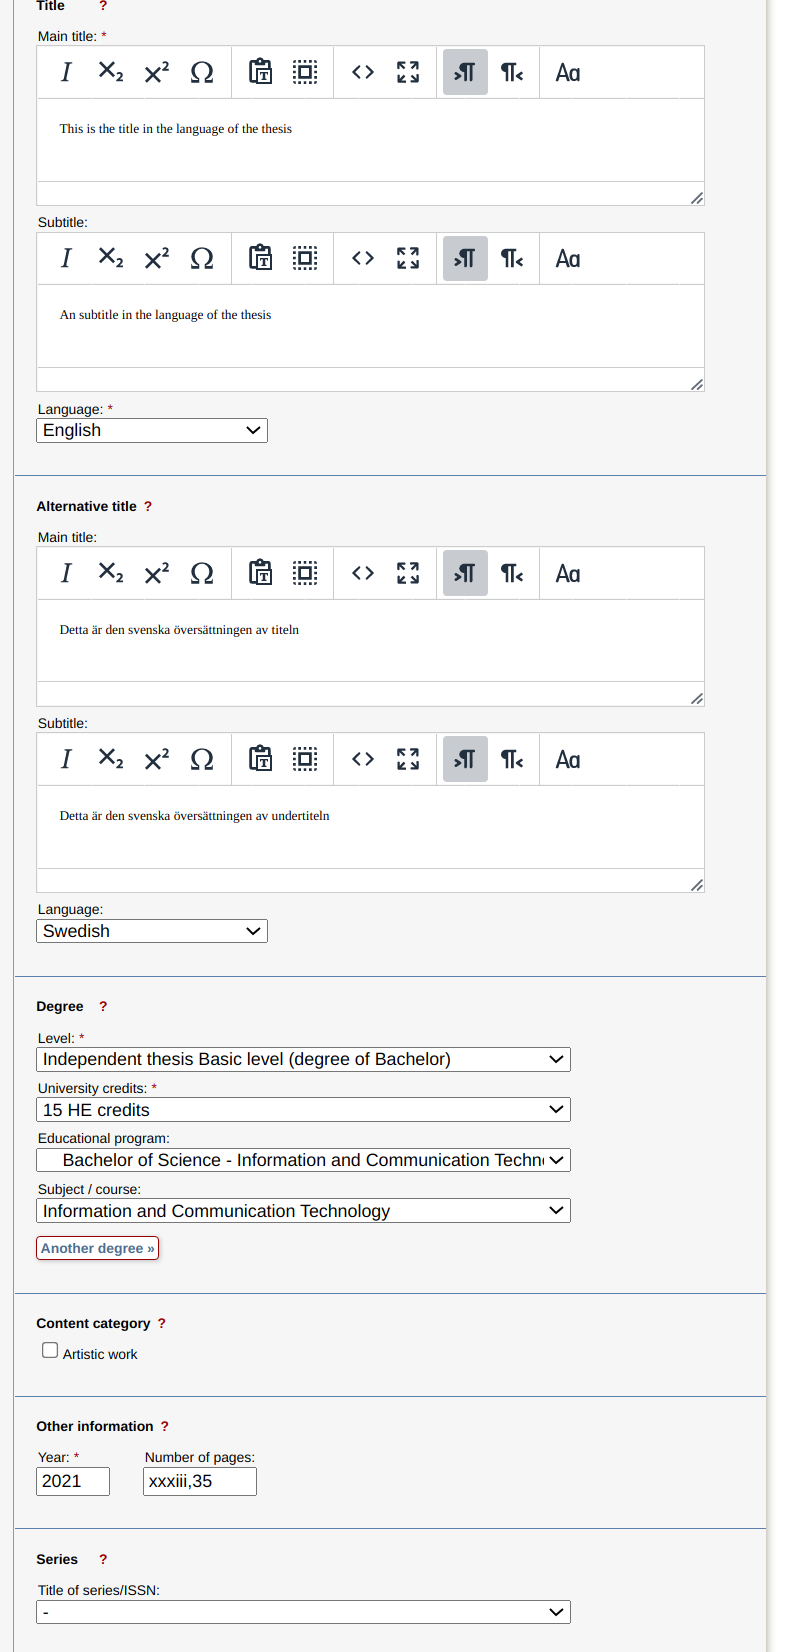
\includegraphics[width=0.65\textwidth]{README_notes/README-examiner-figures/import-b-Screenshot_20210626_234640.png}}
  \end{center}
  \caption[Imported document (part 2)]{Imported document (part 2) – Note that both the English and Swedish titles are shown as well as the information about which level, the number of university credits, the education al program, and the subject.- Additionally, the year and number of pages are shown.}
  \label{fig:divaImport6}
\end{figure}
\FloatBarrier

\begin{figure}[!ht]
  \begin{center}
    \fbox{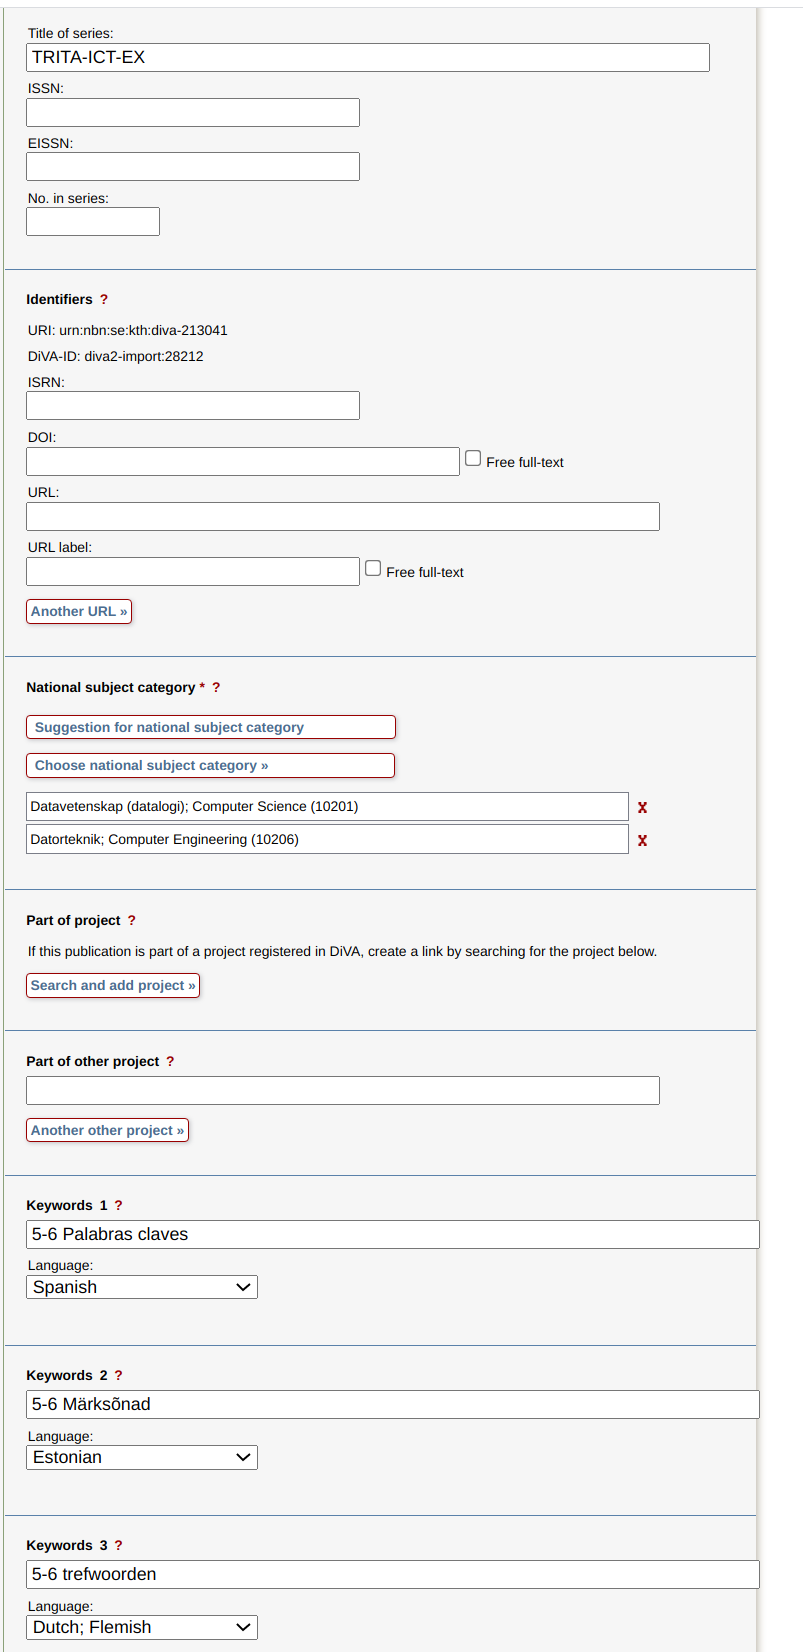
\includegraphics[width=0.65\textwidth]{README_notes/README-examiner-figures/import-c-Screenshot_20210626_234710.png}}
  \end{center}
  \caption[Imported document (part 3)]{Imported document (part 3) – Note that the number in the series is not being shown. The nation subject catergies specified in the JSON file are shown. Additionally, a number of the keyoards in different languages are shown.}
  \label{fig:divaImport7}
\end{figure}
\FloatBarrier

\begin{figure}[!ht]
  \begin{center}
    \fbox{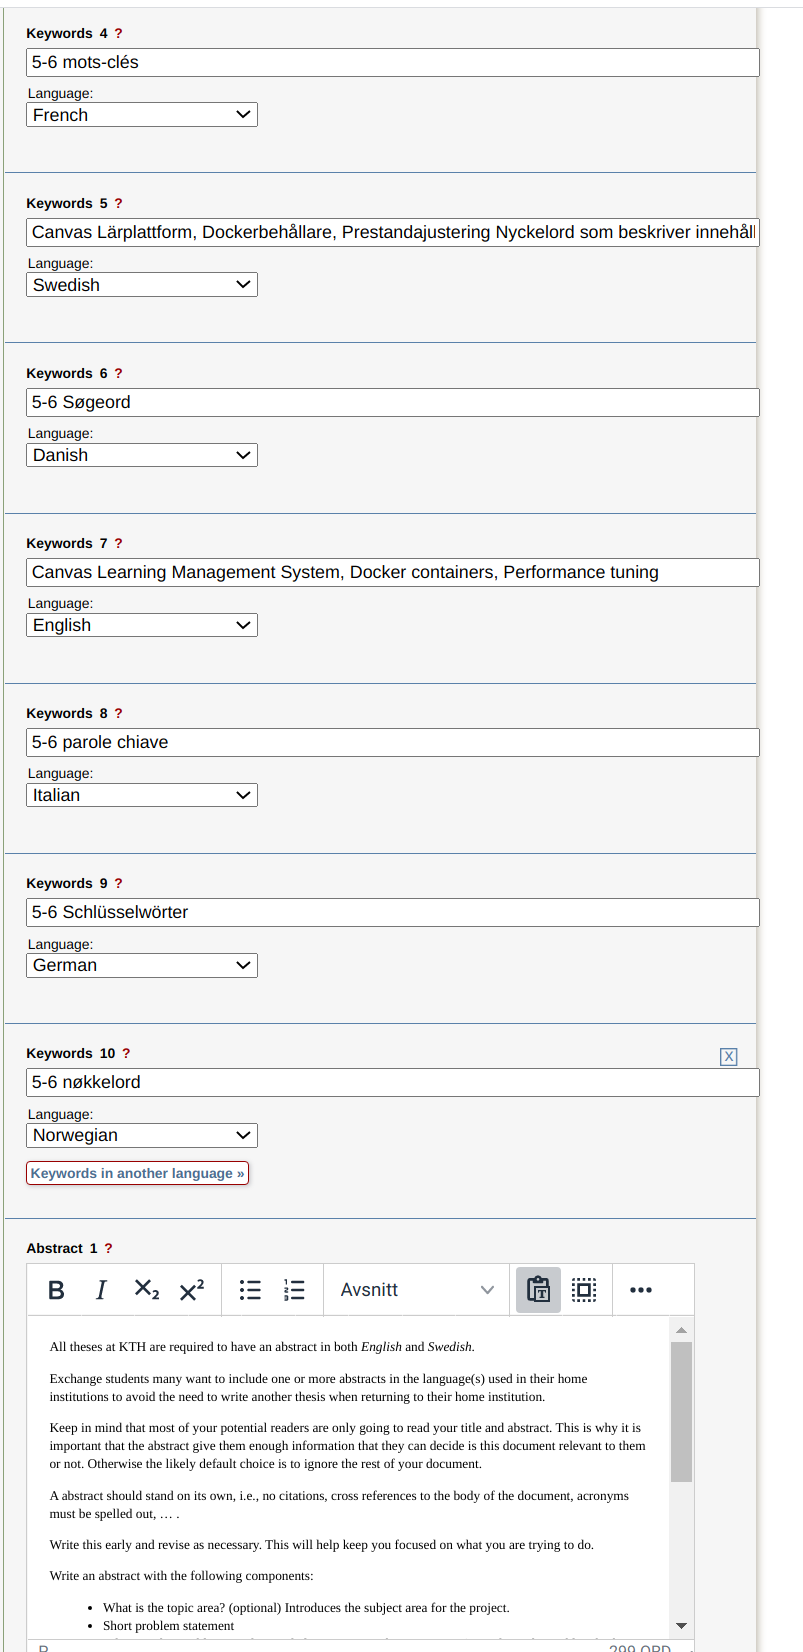
\includegraphics[width=0.65\textwidth]{README_notes/README-examiner-figures/import-d-Screenshot_20210626_234735.png}}
  \end{center}
  \caption[Imported document (part 4)]{Imported document (part 4) – more keywords are shown as well as the abstract in English}
  \label{fig:divaImport8}
\end{figure}
\FloatBarrier

\begin{figure}[!ht]
  \begin{center}
    \fbox{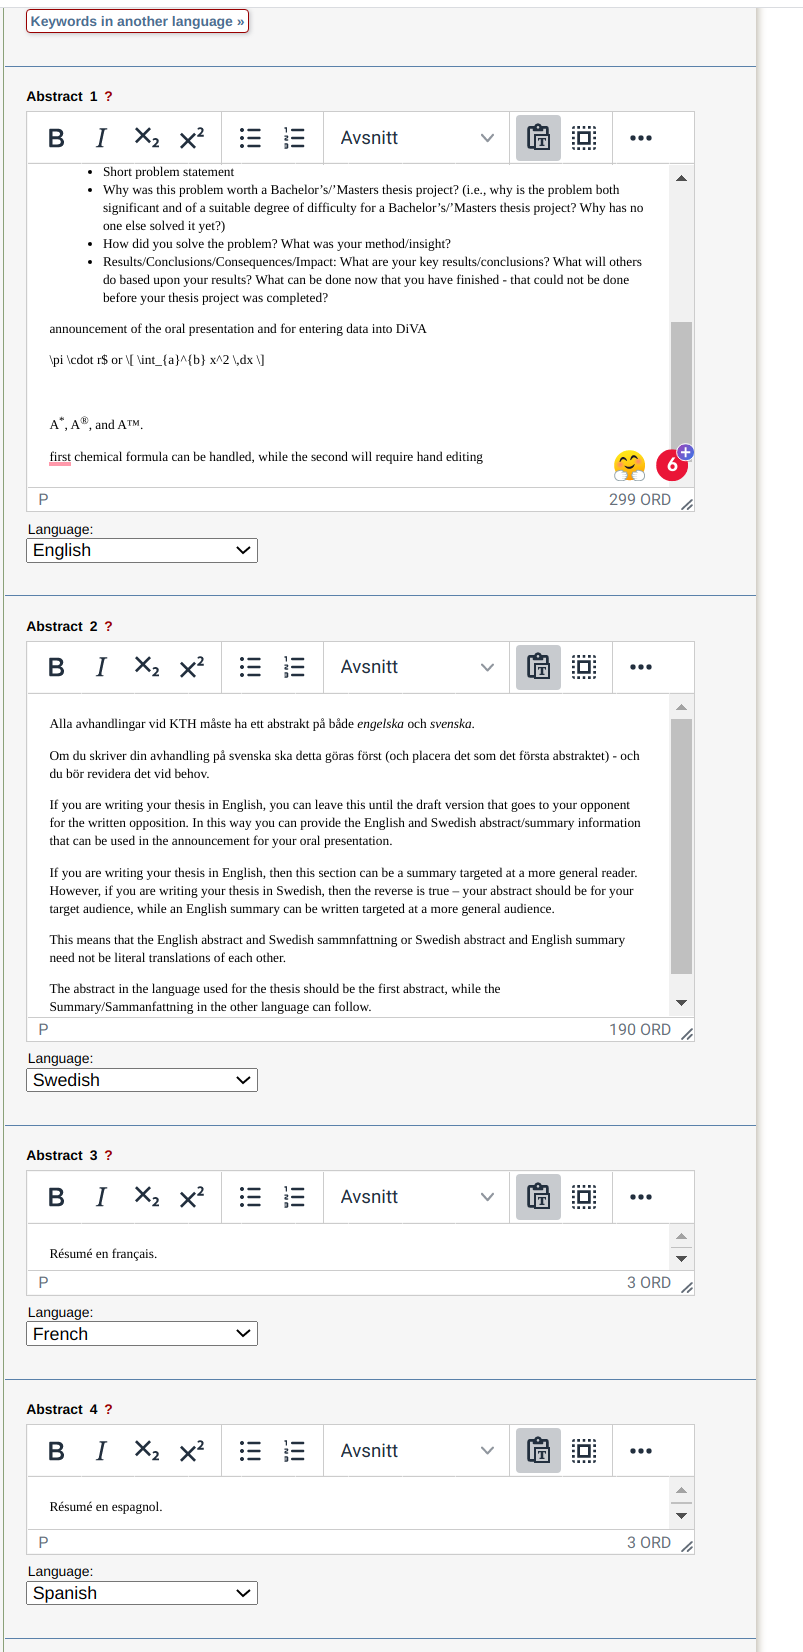
\includegraphics[width=0.65\textwidth]{README_notes/README-examiner-figures/import-e-Screenshot_20210626_235408.png}}
  \end{center}
  \caption{[Imported document (part 5)]Imported document (part 5) – the bottom of the Engish abstract is shown .- showing some of the formatted information that can be shown. Additionally, the Swedish and other abstracts are shown.}
  \label{fig:divaImport9}
\end{figure}
\FloatBarrier

\begin{figure}[!ht]
  \begin{center}
    \fbox{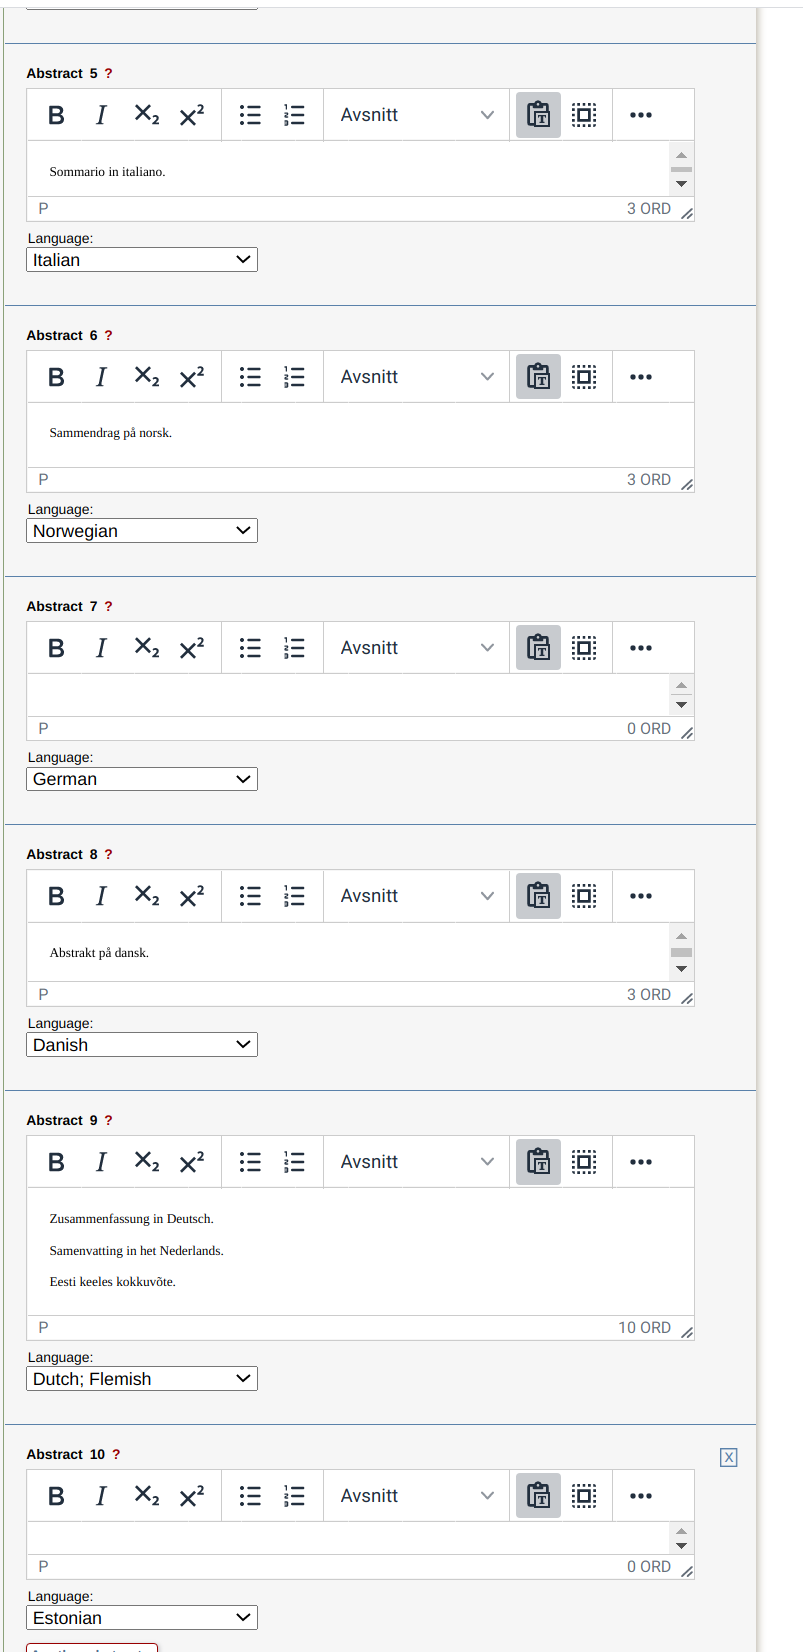
\includegraphics[width=0.7\textwidth]{README_notes/README-examiner-figures/import-f-Screenshot_20210626_235447.png}}
  \end{center}
  \caption[Imported document (part 6)]{Imported document (part 6) – yet more abstracts}
  \label{fig:divaImport10}
\end{figure}
\FloatBarrier
\Cref{fig:divaImport11} shows the three supervisors. The first two have KTH affiliations and the third is from an external organization.
\begin{figure}[!ht]
  \begin{center}
    \fbox{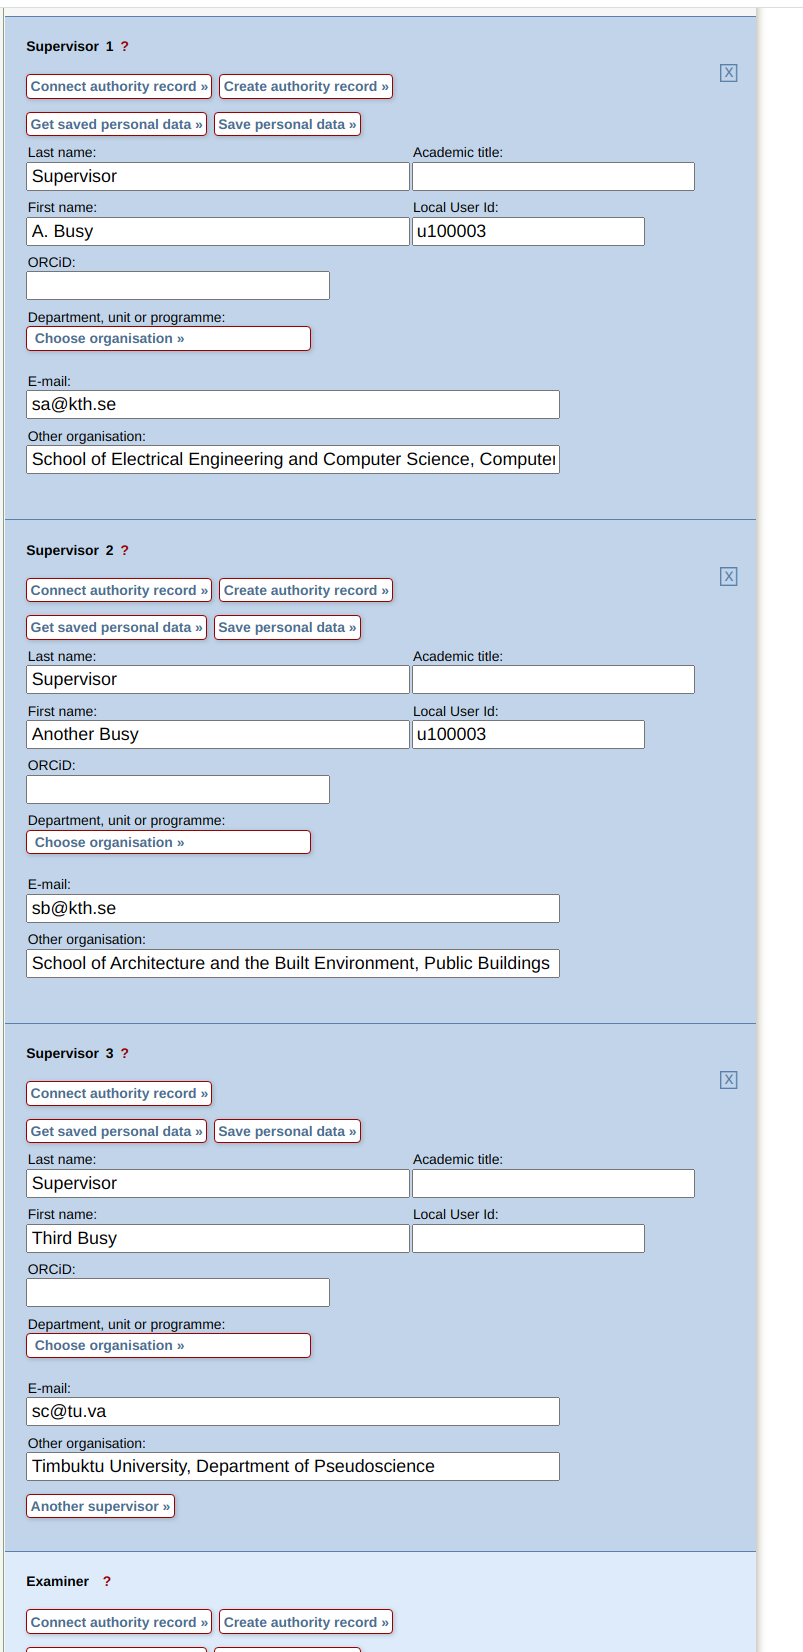
\includegraphics[width=0.7\textwidth]{README_notes/README-examiner-figures/import-g-Screenshot_20210626_235510.png}}
  \end{center}
  \caption[Imported document (part 7)]{Imported document (part 7) – the supervisors are shown}
  \label{fig:divaImport11}
\end{figure}
\newpage

\begin{figure}[!ht]
  \begin{center}
    \fbox{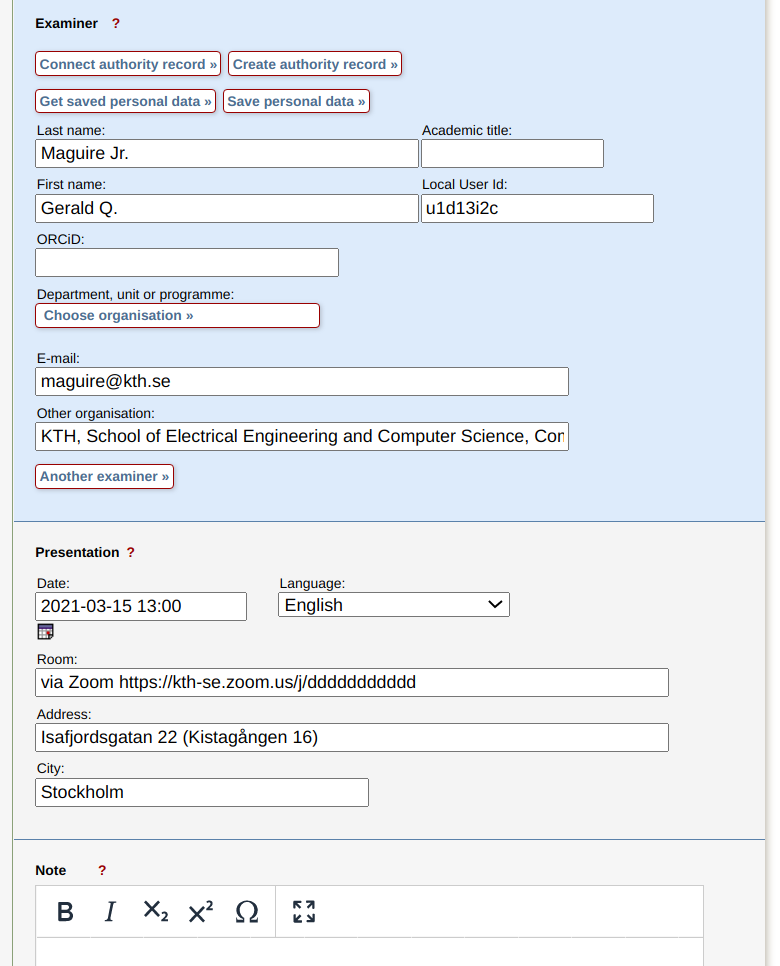
\includegraphics[width=1\textwidth]{README_notes/README-examiner-figures/import-h-Screenshot_20210626_235557.png}}
  \end{center}
  \caption[Imported document (part 8)]{Imported document (part 8) – the examiner is shown along with the information about the oral presentation}
  \label{fig:divaImport12}
\end{figure}
\clearpage


	

\subsection{Limitations}
I was initially unable to get the KTH affiliations correctly entered. I think that it is because I did not understand the description of how to do this at: \url{ https://wiki.epc.ub.uu.se/pages/viewpage.action?pageId=27466001}  where it says:
\babelpolyLangStart{swedish}
För att göra en sådan koppling skall dels ”affiliation” finnas i personelementet dels ett name-element med ID i xlink:href samt ett namePart-element med samma namn som affiliation. Om man har bägge nedanstående element i exemplet kommer Urban Ericsson automatiskt att kopplas till Universitetsbiblioteket i Uppsala vid importen. Om enbart personelementet finns men inte det andra kommer Urban Ericsson att få Uppsala universitet, Universitetsbiblioteket som ”Annat lärosäte” vid importen.
\babelpolyLangStop{swedish}
I did not find any examples of how to do what they describe. The result is that all of my affiliations information ended up in the "Other university" field.

I was also unable to get the issue number to appear, even though it seems to be set - since if you click on the box after the MODS import, it knows the value.  Note that for testing, I forced the TRITA series to be "TRITA-ICT-EX" since this is the actual series that is in the earlier (test) version of DiVA.

Finally, it seems that DiVA does not import the cooperation data at all: according to \url{https://wiki.epc.ub.uu.se/display/divainfo/Externt+samarbete}

The first two limitations have been overcome as described in\linebreak[4] \Cref{sec:limitationsOvercome}.

\subsection{Limitations overcome}
\label{sec:limitationsOvercome}
This section describes how two of the limitations were overcome.

\subsubsection{Entering number in series}
The first limitation to be over come was entering the particular number in the series for a TRITA number. \Cref{fig:numberInSeriesCorrectlyEntered} shows the value being entered. The error was in the structure of the object, the working version is shown in \Cref{lst:seriesNumber}. My earlier error was due to having the \texttt{<identifier type="issue number">2021:00</identifier>} \textit{within} the \texttt{<titleInfo>}.
 
 
\begin{figure}[!ht]
  \begin{center}
    \fbox{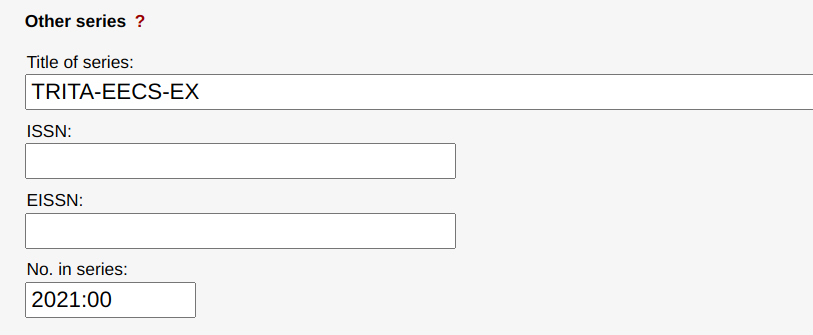
\includegraphics[width=1\textwidth]{README_notes/README-examiner-figures/Number_in_series_correctly_entered.png}}
  \end{center}
  \caption{Number in series correctly entered}
  \label{fig:numberInSeriesCorrectlyEntered}
\end{figure}
\Needspace*{8\baselineskip}
\begin{lstlisting}[language={XML}, caption={MODS data for series}, label=lst:seriesNumber]
<relatedItem  type="series">
	      <titleInfo><title>TRITA-EECS-EX</title>
		<identifier type="local">16855</identifier>
	      </titleInfo>
	      <identifier type="issue number">2021:00</identifier>
</relatedItem >
\end{lstlisting}

\FloatBarrier

\subsubsection{Including KTH affiliations}
Earlier, those with KTH affiliations were appearing in the “Other organization” field. The error in my understanding was how the controlled fields for the KTH authors was being used\footnote{These so-called "controlled" fields have specific values that are permitted and these have numeric IDs assigned by the DiVA Consortium.}. We will start by looking at the two KTH affiliated supervisors (see \Cref{fig:twoKTHsupervisors}), the third supervisor (see \Cref{fig:thirdSupervisor}), and the examiner (see \Cref{fig:examiner}). The MODS data for these four people is shown in \Cref{lst:reducedModesExaminerAndSupervisors} and the “magic” \textbf{corporate name} MODS data is shown in \Cref{lst:reducedModesCorpNames}. The trick is that there needs to be corporate name MODS data for each of the possible affiliations – as this is the way that one passes the DiVA numeric code via the \texttt{xlink} information. Note that in the case of the examiner, two different affiliations were specified and there was a corporate name entry for each of them. Moreover, the key is just to have test extra corporate name entries, only one needs to be for the publishers, as shown in \Cref{lst:reducedModesCorpNames} – with the results in \Cref{fig:twoSupervisorsReducedMODS} and shown \Cref{fig:examinerReducedMODS}.

\textbf{NB}: The ICT affiliations (and DiVA codes) were used and the pictures are all from the test DiVA environment: \url{https://kth.test.diva-portal.org/dream/import/importList.jsf}.

\begin{figure}[!ht]
  \begin{center}
    \fbox{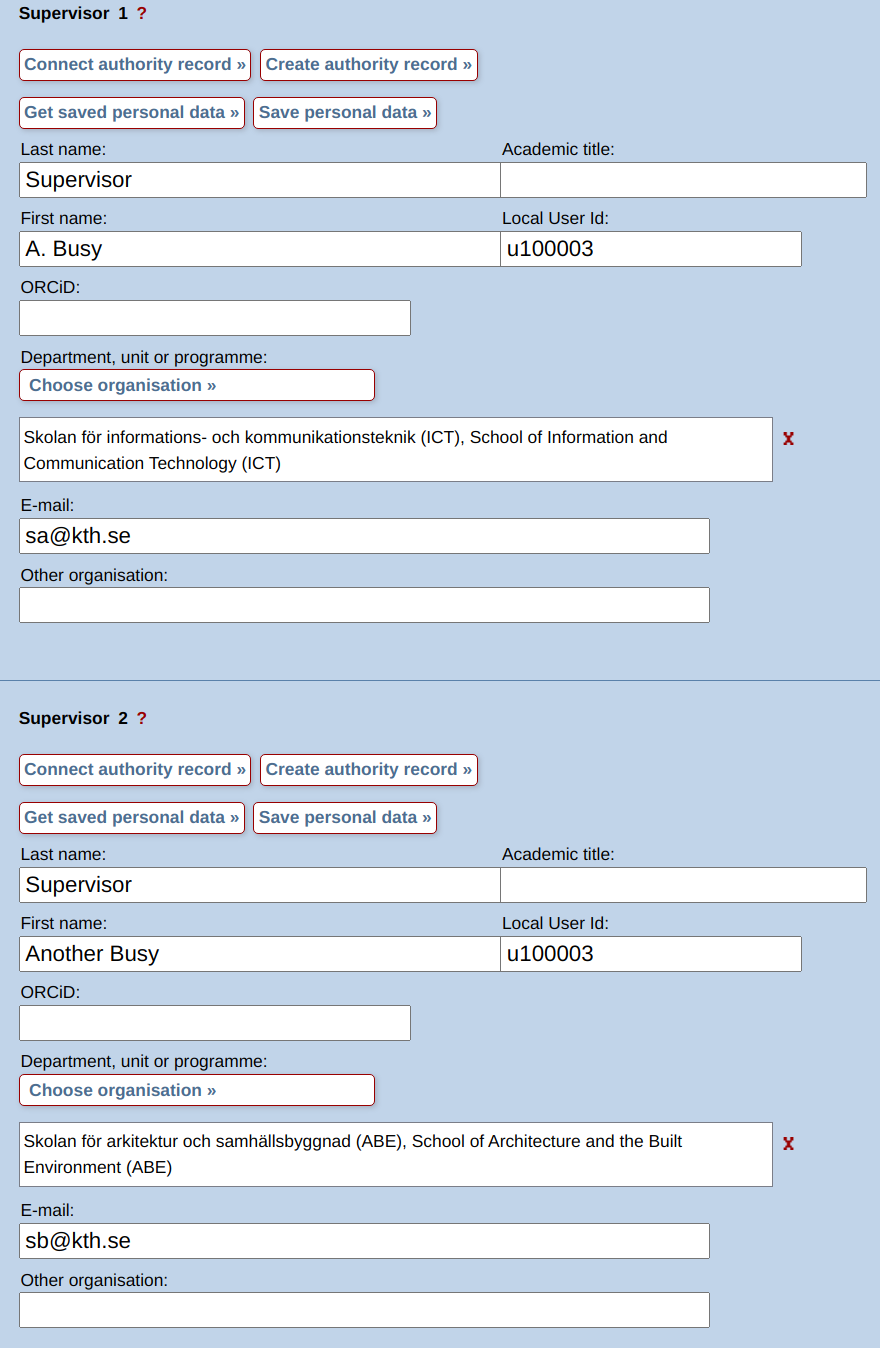
\includegraphics[width=0.9\textwidth]{README_notes/README-examiner-figures/two_KTH_supervisors_in_different_schools.png}}
  \end{center}
  \caption{Two KTH supervisors in different schools}
  \label{fig:twoKTHsupervisors}
\end{figure}
\FloatBarrier
\begin{figure}[!ht]
  \begin{center}
    \fbox{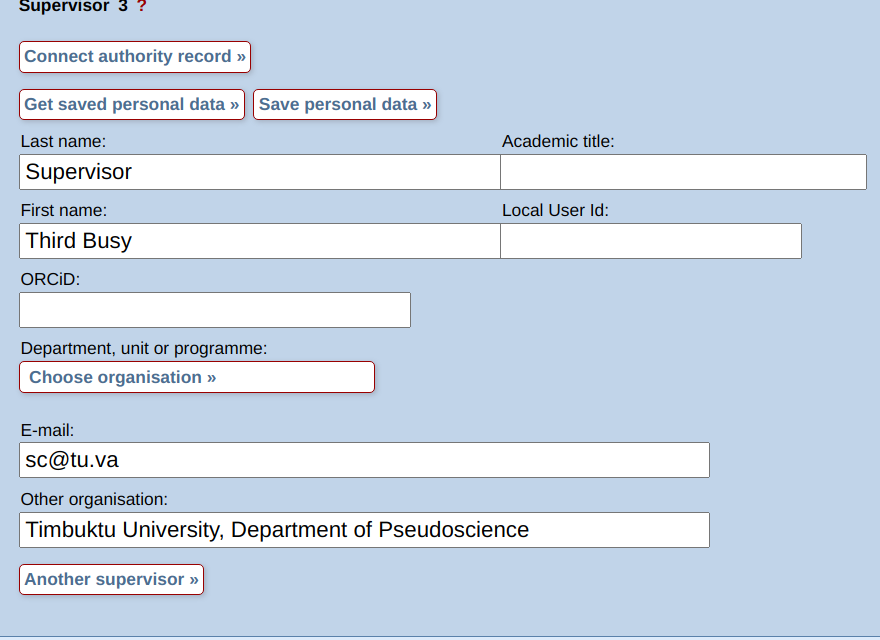
\includegraphics[width=1\textwidth]{README_notes/README-examiner-figures/third_supervisor.png}}
  \end{center}
  \caption{Third supervisor}
  \label{fig:thirdSupervisor}
\end{figure}
\FloatBarrier
\begin{figure}[!ht]
  \begin{center}
    \fbox{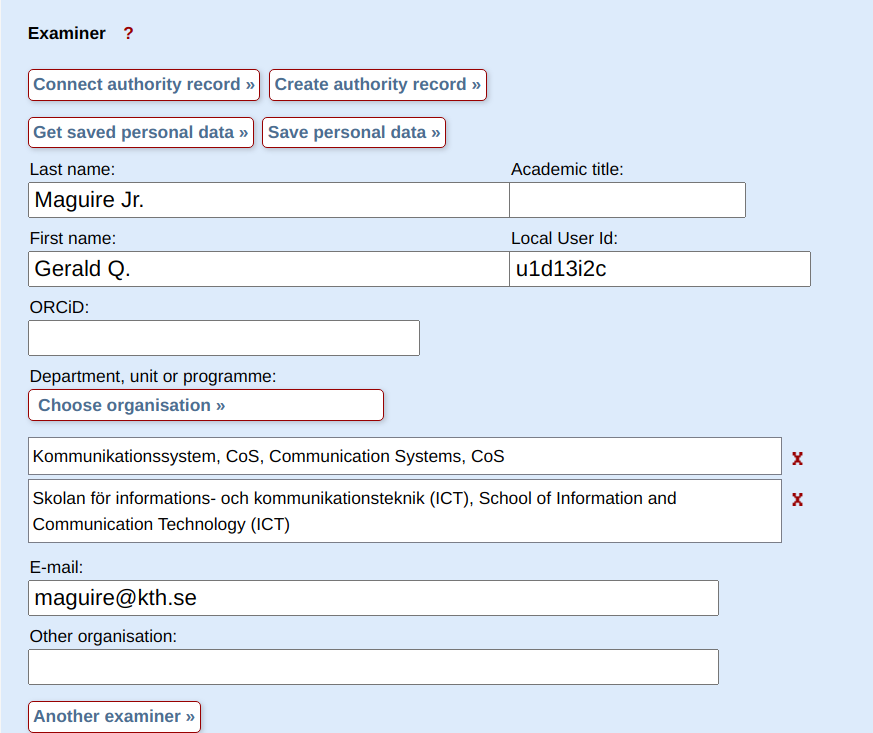
\includegraphics[width=1\textwidth]{README_notes/README-examiner-figures/examiner_affiliation.png}}
  \end{center}
  \caption{Examiner}
  \label{fig:examiner}
\end{figure}
\clearpage

\begin{lstlisting}[language={XML}, caption={MODS data for the supervisors and examiners}, label=lst:reducedModesExaminerAndSupervisors]
<name type="personal" authority="kth" xlink:href="u1d13i2c">
      <namePart type="family">Maguire Jr.</namePart>
      <namePart type="given">Gerald Q.</namePart>
      <description>email=maguire@kth.se</description>
      <affiliation>KTH, Skolan för informations- och kommunikationsteknik (ICT), Kommunikationssystem, CoS</affiliation>
      <affiliation>KTH, Skolan för informations- och kommunikationsteknik (ICT)</affiliation>
      <role><roleTerm type="code" authority="marcrelator">mon</roleTerm></role>
</name>

<name type="personal" authority="kth" xlink:href="u100003">
      <namePart type="family">Supervisor</namePart>
      <namePart type="given">A. Busy</namePart>
      <affiliation>KTH, Skolan för informations- och kommunikationsteknik (ICT)</affiliation>
      <description>email=sa@kth.se</description>
      <role><roleTerm type="code" authority="marcrelator">ths</roleTerm></role>
</name>

<name type="personal" authority="kth" xlink:href="u100003">
      <namePart type="family">Supervisor</namePart>
      <namePart type="given">Another Busy</namePart>
      <affiliation>KTH, Skolan för arkitektur och samhällsbyggnad (ABE)</affiliation>
      <description>email=sb@kth.se</description>
      <role><roleTerm type="code" authority="marcrelator">ths</roleTerm></role>
</name>

<name type="personal">
      <namePart type="family">Supervisor</namePart>
      <namePart type="given">Third Busy</namePart>
      <affiliation>Timbuktu University, Department of Pseudoscience</affiliation>
      <description>email=sc@tu.va</description>
      <role><roleTerm type="code" authority="marcrelator">ths</roleTerm></role>
</name>
\end{lstlisting}
\clearpage

\begin{lstlisting}[language={XML}, caption={Corporate name data in MODS data for the affiliations}, label=lst:reducedModesCorpNames]
<name type="corporate" authority="kth" xlink:href="5994">
      <namePart>KTH</namePart>
      <namePart>Skolan för informations- och kommunikationsteknik (ICT)</namePart>
      <role><roleTerm type="code" authority="marcrelator">pbl</roleTerm></role>
</name>

<name type="corporate" authority="kth" xlink:href="5998">
      <namePart>KTH</namePart>
      <namePart>Skolan för informations- och kommunikationsteknik (ICT)</namePart>
      <namePart>Kommunikationssystem, CoS</namePart>
      <role><roleTerm type="code" authority="marcrelator">pbl</roleTerm></role>
</name>

<name type="corporate" authority="kth" xlink:href="5850">
      <namePart>KTH</namePart>
      <namePart>Skolan för arkitektur och samhällsbyggnad (ABE)</namePart>
      <role><roleTerm type="code" authority="marcrelator">pbl</roleTerm></role>
</name>
\end{lstlisting}

\begin{lstlisting}[language={XML}, caption={Reduced MODS for corporate names more}, label=lst:reducedModesCorpNamesMore]
<name type="corporate" authority="kth" xlink:href="5994">
      <namePart>KTH</namePart>
      <namePart>Skolan för informations- och kommunikationsteknik (ICT)</namePart>
      <role><roleTerm type="code" authority="marcrelator">pbl</roleTerm></role>
</name>
<name type="corporate" authority="kth" xlink:href="5998">
      <namePart>KTH</namePart>
      <namePart>Skolan för informations- och kommunikationsteknik (ICT)</namePart>
      <namePart>Kommunikationssystem, CoS</namePart>
</name>
<name type="corporate" authority="kth" xlink:href="5850">
      <namePart>KTH</namePart>
      <namePart>Skolan för arkitektur och samhällsbyggnad (ABE)</namePart>
</name>
\end{lstlisting}
\clearpage

\begin{figure}[!ht]
  \begin{center}
    \fbox{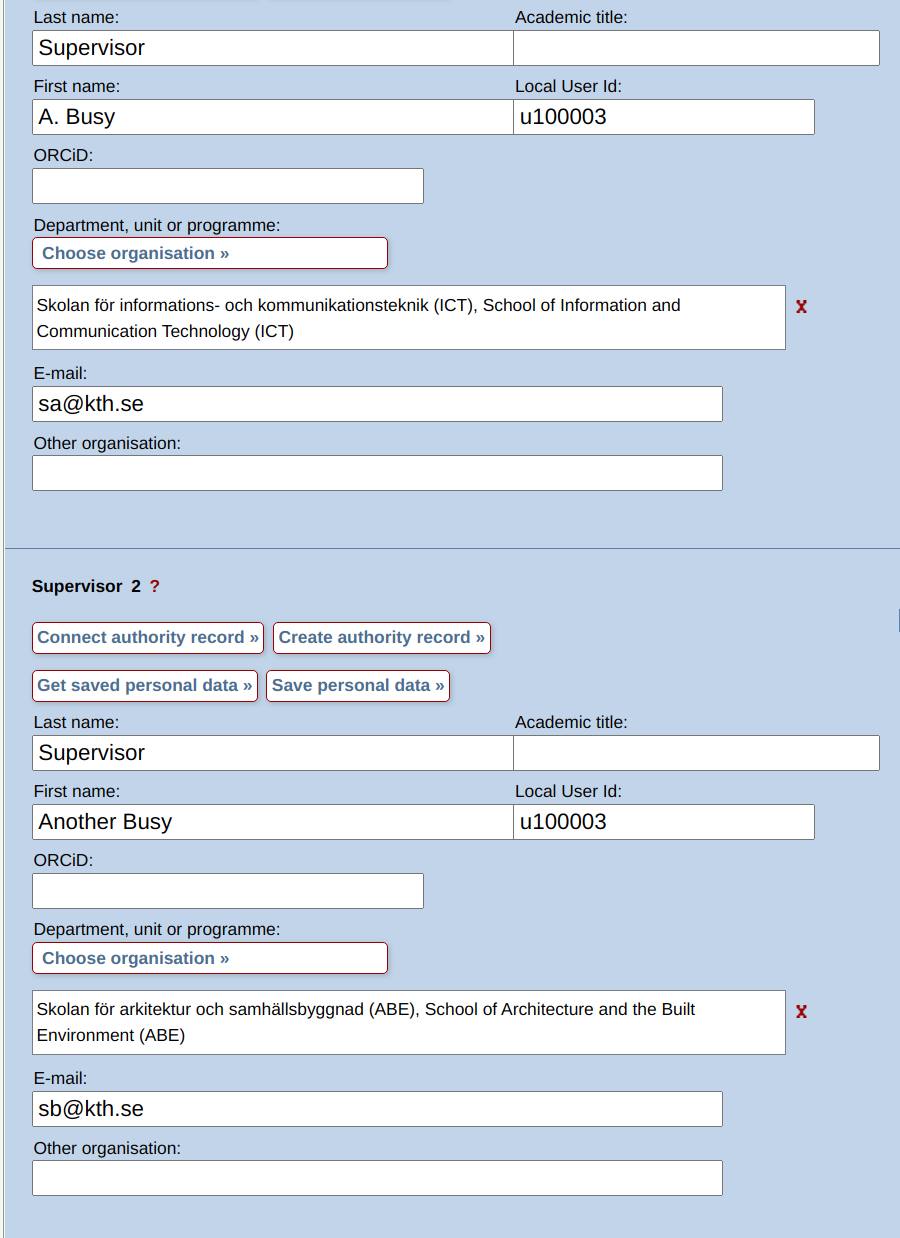
\includegraphics[width=1\textwidth]{README_notes/README-examiner-figures/two_supervisors_reduced_mods.png}}
  \end{center}
  \caption{The two supervisors with the reduced MODS for corporate names}
  \label{fig:twoSupervisorsReducedMODS}
\end{figure}

\begin{figure}[!ht]
  \begin{center}
    \fbox{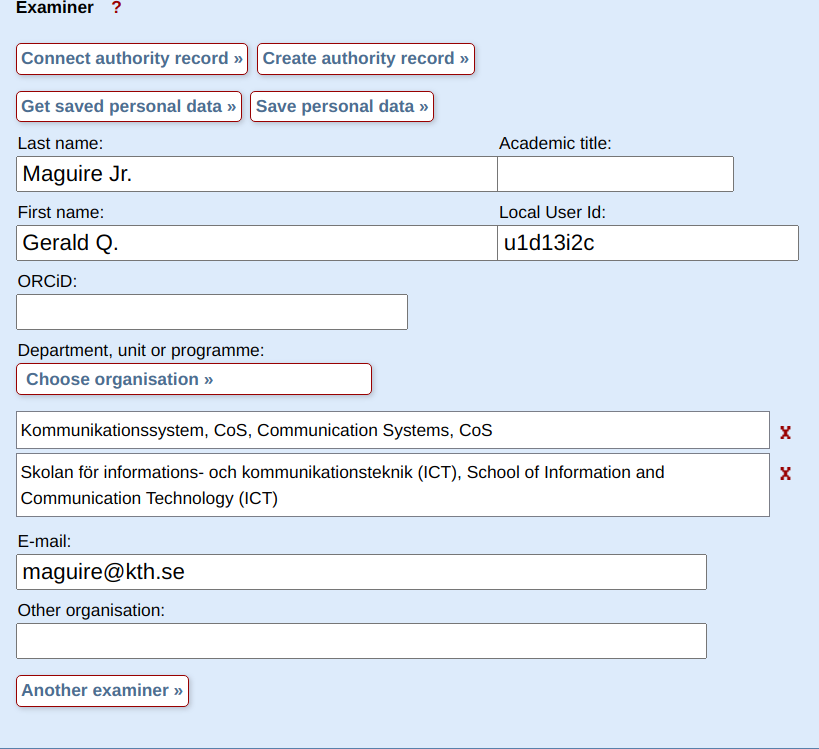
\includegraphics[width=1\textwidth]{README_notes/README-examiner-figures/examiner_with_reduced_mods.png}}
  \end{center}
  \caption{The examiner with the reduced MODS for corporate names}
  \label{fig:examinerReducedMODS}
\end{figure}
\clearpage

\section{Some enhancements}
\label{sec:someEhnahncements}
The enhancements described in \Cref{sec:enhancementsToTemplate} are enhancements to the template and supporting programs to avoid the user having to enter some information on the command line when making a cover and to make the information better available for a future DiVA entry. The enhancements described in \Cref{sec:betterSupportForMathInAbstracts} are to better support mathematical expressions in abstracts. \Cref{sec:AcronymsInAbstracts} describes support for acronyms in abstracts. \Cref{sec:URLSinAbstracts} describes the state of support for URLs in abstracts. \Cref{sec:gettingPDFfromCanvasAssignment} describes a program that can extract an assignment from a Canvas course room and optionally feed it to the program to extract the pseudo-JSON information.

\subsection{Enhancements to template and supporting programs}
\label{sec:enhancementsToTemplate}
Add better support for the subject area (or areas in the case of a student doing both a Civ. Ing. Degree and a Master’s degree).

\subsection{Better support for mathematical expressions in abstracts}
\label{sec:betterSupportForMathInAbstracts}
\LaTeX~in the abstracts is passed through to the pseudo JSON in the “For DIVA” text at the end of the thesis. When preparing this text for Cortina calendar entries or for the announcement in the Canvas course room (and for the calendar event in the course room) some simple \LaTeX~commands are converted to HTML. As few abstracts (in the many abstracts that I looked at in DiVA) have equations I have only done these few transformations. However, if there were to be more use of equations, then there is probably a need to support them for the different platforms (Cortina (see Appendix~\ref{sec:BetterSupportforMathinCortina}), DiVA (see Appendix~\ref{sec:SupportForMathematicsInDiVA}), and Canvas (see Appendix~\ref{sec:betterSupportMathInCortinaAndCourseCalendar})).


\subsubsection{Better support for mathematics in Canvas course announcement and course calendar}
\label{sec:betterSupportMathInCortinaAndCourseCalendar}
As of 2021-06-18, MathJAX and URLs are now supported in the Canvas course room announcement and calendar.
Using the Overleaf project: \url{https://www.overleaf.com/read/qsyddnhhvkgr} to provide a test source document. The results can be seen in \Cref{fig:equationsInAnnouncement}. These results and the results shown in Appendix~\ref{sec:BetterSupportforMathinCortina} were generated using the commands in \Cref{lst:jsonToCalendar3}.
\begin{figure}[!ht]
  \begin{center}
    \fbox{
\includegraphics[width=1\textwidth]{README_notes/README-examiner-figures/announcement_with_equation.png}}
  \end{center}
  \caption{Examples of equations in an announcement}
  \label{fig:equationsInAnnouncement}
\end{figure}
\FloatBarrier
\Needspace*{8\baselineskip}
\begin{lstlisting}[language={bash}, caption={Commands to produce the JSON and make the calendar entries and announcement}, label=lst:jsonToCalendar3]
./extract_pseudo_JSON-from_PDF.py --pdf abstracts_with_equations_in_them.pdf --json eqtest.json
./JSON_to_calendar.py -c 11 --config config-test.json --json eqtest.json
\end{lstlisting}

\FloatBarrier

Note that block/display math are displayed in the Canvas summary for the announcements and cause Canvas to stop summarizing the abstract. The cause for this is not yet known, but has been reported to e-learning ([\#ID:KTH-INC-3677258\#]) and I have blogged about it in the Canvas Community. An example of the equation being displayed in the summary of the announcement is shown in \Cref{fig:announcementSummary}. The announcement is shown in \Cref{fig:announcementWithEquation} while \Cref{lst:HTMLannouncement} shows the HTML for this announcement.

\begin{figure}[!ht]
  \begin{center}
    \fbox{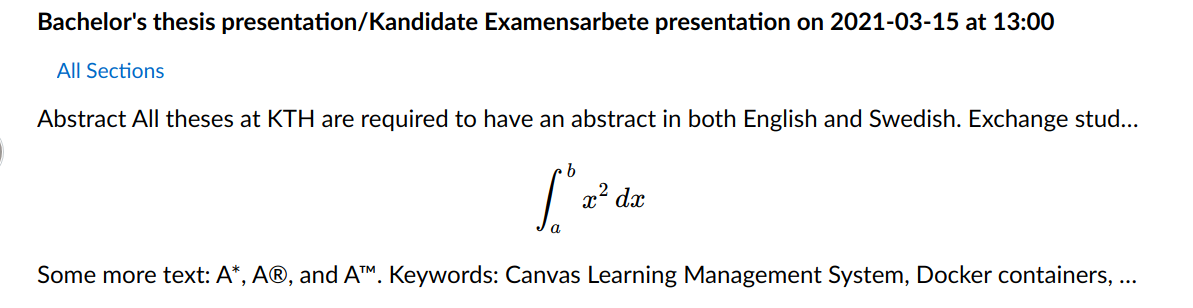
\includegraphics[width=1\textwidth]{README_notes/README-examiner-figures/Announcement_summary.png}}
  \end{center}
  \caption{Announcement summary}
  \label{fig:announcementSummary}
\end{figure}
\FloatBarrier

\begin{figure}[!ht]
  \begin{center}
    \fbox{
\includegraphics[width=1\textwidth]{README_notes/README-examiner-figures/announcement_with_equation.png}}
  \end{center}
  \caption{Announcement with equation}
  \label{fig:announcementWithEquation}
\end{figure}
\FloatBarrier
\Needspace*{18\baselineskip}
\begin{lstlisting}[language={HTML}, caption={HTML for the announcement}, label=lst:HTMLannouncement]
<h2 lang="en">Abstract</h2>
<p>All theses at KTH are required to have an abstract in both <i>English</i> and <i>Swedish</i>.</p>
<p>Exchange students many want to include one or more abstracts in the language(s) used in their home institutions to avoid the need to write another thesis when returning to their home institution.</p>
<p><span class="math-tex">\(\pi \cdot r\)</span> or <span class="math-tex">\[ \int_{a}^{b} x^2 \,dx \]</span></p>
<p>Some more text: A<sup>*</sup>, A<sup>&reg;</sup>, and A&trade;.</p>
<p><strong>Keywords:</strong> <em>Canvas Learning Management System, Docker containers, Performance tuning </em></p>
\end{lstlisting}


Via XXXXX at IT-support, I raised the question about why the block equations were appearing in the summary of the announcement.

The response from Instructure support regarding the block equations showing up in the summary of the announcements was\footnote{Note that the URLs have been added in parenthesis.}:
\begin{quote}
Thank you for reaching back out.  I did some testing on this and I have a few things to point out and some follow up questions.

First off, the syntax of the block equation isn't the officially supported format.  The inline equation is correct with the \textbackslash(...\textbackslash) delimiters, but the block equation should be formatted with dollar signs, as \$\$...\$\$.  I see the square bracket delimiters \textbackslash[...\textbackslash] are working currently, but this is not the officially supported format and may not always work.  Information on this can be found in these release notes (\url{https://community.canvaslms.com/t5/Canvas-Releases/Canvas-Release-Notes-2021-02-20/ta-p/434781\#toc-hId-698876024}).

Regardless of that though, I wanted to get clarification on the issue at hand.  When I open the announcement, I see both the inline and block equations, but I see only the block equation when viewing it on the main Announcements page.  Is this specifically what you're reporting?  (sandbox screenshot for reference (\url{https://share.getcloudapp.com/jkuPOKRD})  If so, this is because the Announcements page only shows a snippet of the text, so an inline equation beyond the point the text is truncated isn't treated any differently than the rest of the text not shown.  It is interesting that Canvas decides to show the block equation in this view though.  Having that removed from the preview would best be submitted as a feature request (\url{https://community.canvaslms.com/t5/forums/postpage/board-id/ideas/search-before-post-mode/true} ).

If the issues you're reporting are when the full announcement is open, I'm not seeing the same behavior on this end.  If that's the case, can you provide a screenshot of what you're seeing?  And does the behavior persist in a different browser?

Let me know if I've misinterpreted anything or if there are any other questions as well.  We'll be happy to help.  Thanks and have a great day!"
\end{quote}

The response from someone at Instructure shows that Instructure got the same behavior from the block equations in the snippets of the announcements.  A screenshot of this behavior is shown in \Cref{fig:screenSHotOfBlockEquation}. However, their solution for this is to suggest that we submit a feature request. 

\begin{figure}[!ht]
  \begin{center}
    \fbox{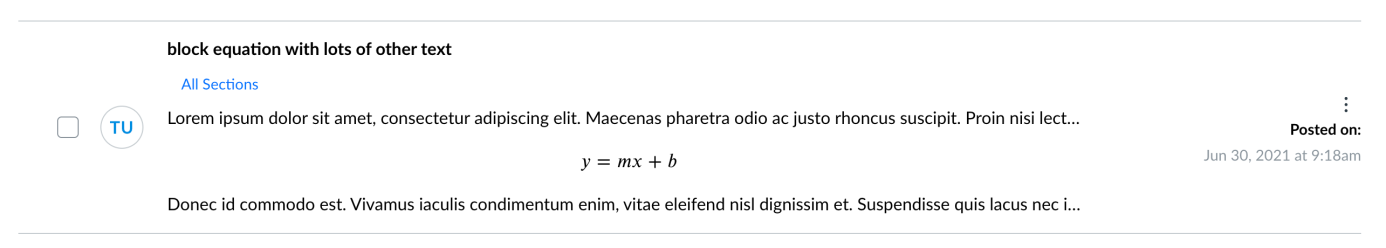
\includegraphics[width=1\textwidth]{README_notes/README-examiner-figures/block_equation_in_Canvas.png}}
  \end{center}
  \caption{The screenshot mentioned above}
  \label{fig:screenSHotOfBlockEquation}
\end{figure}
\FloatBarrier



\subsubsection{Better support for mathematics in Cortina}
\label{sec:BetterSupportforMathinCortina}

YYYYYY indicated that CORTINA supports mathematical expressions using a class name of “math-tex” and gave an example:
%% <span class=\"math-tex\">\\(x = {-b \\pm \\sqrt{b^2-4ac} \\over 2a}\\)</span>
\begin{quote}
$<$span class=\textbackslash"math-tex\textbackslash"$>$\textbackslash\textbackslash(x = {-b \textbackslash\textbackslash pm \textbackslash\textbackslash sqrt\{b\^{}2-4ac\} \textbackslash\textbackslash over 2a}\textbackslash\textbackslash)$<$/span$>$
\end{quote}


\noindent He also noted that Cortina does not allow images in paragraphs, so the solutions for Cortina and DiVA have to be different.

An important note about the above example is that \textbackslash over is deprecated and one should use \textbackslash frac{}{} or one of its variance instead; hence, I used this version of the equation in my source \LaTeX~file.
\clearpage
\Cref{fig:cortinaExample1} shows the entry in the Cortina calendar, while \Cref{fig:cortinaExample2} and \Cref{fig:cortinaExample3} show zoomed in views of the equations.
\begin{figure}[!ht]
  \begin{center}
    \fbox{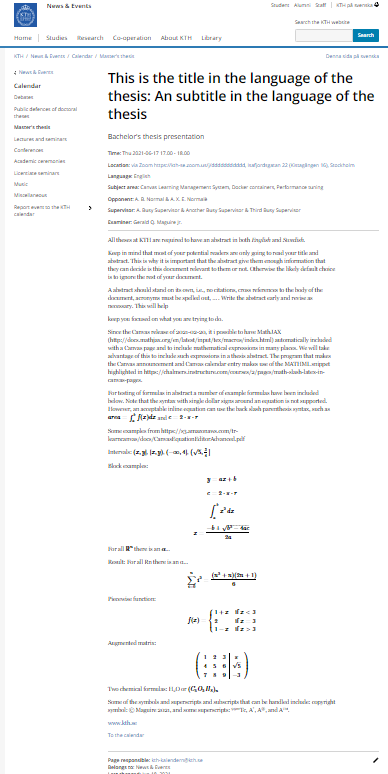
\includegraphics[width=0.65\textwidth]{README_notes/README-examiner-figures/Cortina_exaample1.png}}
  \end{center}
  \caption{Equations in Cortina calendar entry}
  \label{fig:cortinaExample1}
\end{figure}
\FloatBarrier

\begin{figure}[!ht]
  \begin{center}
    \fbox{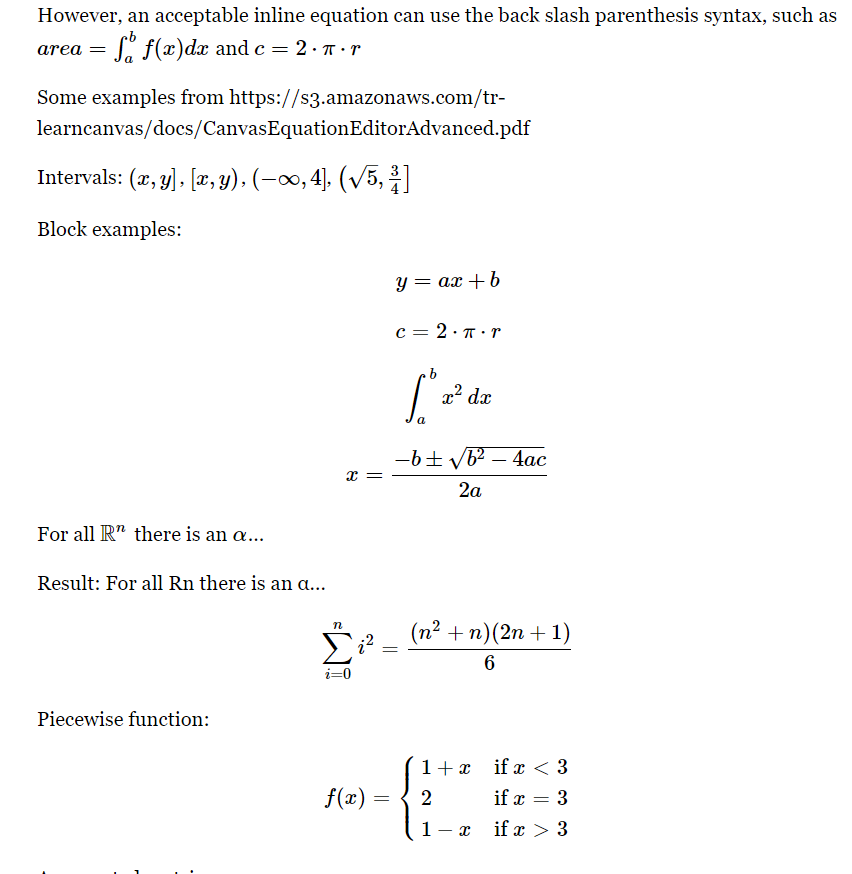
\includegraphics[width=1\textwidth]{README_notes/README-examiner-figures/cortina-eqn-zoom1.png}}
  \end{center}
  \caption{Zoom in on part of the Cortina calendar entry}
  \label{fig:cortinaExample2}
\end{figure}
\FloatBarrier

\begin{figure}[!ht]
  \begin{center}
    \fbox{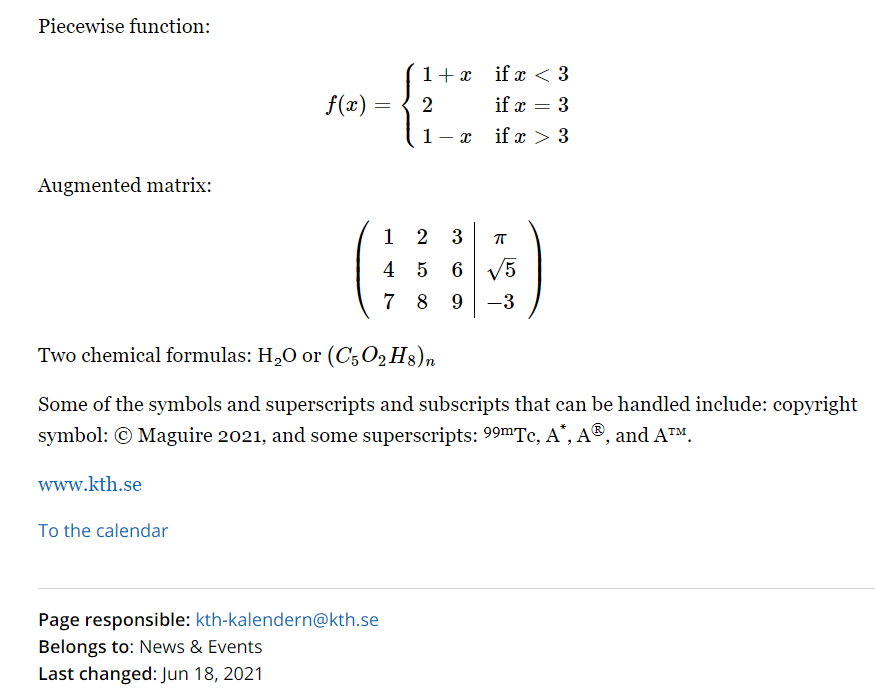
\includegraphics[width=1\textwidth]{README_notes/README-examiner-figures/cortina-eqn-zoom2.png}}
  \end{center}
  \caption{Zoom in on lower part of the Cortina calendar entry}
  \label{fig:cortinaExample3}
\end{figure}
\FloatBarrier
 

\subsubsection{Support for mathematics in DiVA}
\label{sec:SupportForMathematicsInDiVA}
In contrast to Canvas and Cortina, DiVA uses pictures (although these can have a \LaTeX~expression as an “alt” description of the image contents).
The code does not (yet) support the addition of equations to the DiVA entry of the abstracts.
The current DiVA user interface seems to strip out the math-tex classes, \ie 

% <span class='math-tex'>\[ \int_{a}^{b} x^2 \,dx \]</span> 
\begin{quote}
$<$span class=\textbackslash"math-tex\textbackslash"$>$\textbackslash [ \textbackslash int\_\{a\}\^{}\{b\} x\^{}  \textbackslash ,dx \textbackslash ] $<$/span$>$
\end{quote}

becomes simply:
% \[ \int_{a}^{b} x^2 \,dx \]
\begin{quote}
\textbackslash [ \textbackslash int\_\{a\}\^{}\{b\} x\^{}2  \textbackslash ,dx \textbackslash ]
\end{quote}
\noindent However, I do not know what happens when this is later displayed by DiVA, \ie whether it will appear as an equation or not.

Fortunately, one can use the picture support as shown in the example below to generate \textbackslash\ widehat\{Err\} over Err:
\begin{quote}
<img src="http://www.diva-portal.org/cgi-bin/mimetex.cgi?\%5Cwidehat\%7BErr\%7D" data-classname="equation" data-title="" />
\end{quote}

\subsection{Acronyms in abstracts}
\label{sec:AcronymsInAbstracts}

As students may use acronyms in abstracts, there is support for the commands: \textbackslash gls{}, \textbackslash glspl{}, \textbackslash Gls{}, \textbackslash Glspl{}, \textbackslash acrlong{}, \textbackslash acrshort{}, and \textbackslash acrfull{}. There is also an optional argument to the extraction program to specify the name of the file with definitions of acronyms using the \texttt{\textbackslash newacronyms\{label\}\{acronym\}\{phrase\}} form of definitions. This optional argument is shown in \Cref{lst:specifyingAcronymsFile}. Note that expanding acronyms are handled independently for the abstracts, so that they are spell out on first use in each abstract. Note also that there is no support for multiple languages for the phrase that is used, \ie the expansion simply uses the phrase defined in the \textbackslash newacronyms definition.
\Needspace*{4\baselineskip}
\begin{lstlisting}[language={bash}, caption={Specifying acronyms file}, label=lst:specifyingAcronymsFile]
./extract_pseudo_JSON-from_PDF.py --pdf xxxx.pdf --json xxxx.json --acronyms acronyms.tex
\end{lstlisting}


Additionally, the commands (from \texttt{defines.tex}) are supported in abstracts: \textbackslash ie, \textbackslash eg, \textbackslash etc, \textbackslash etal, \textbackslash first, \textbackslash second, \textbackslash third, \ldots . Now that all the acronyms are spelled out, there is no problem with them when making a calendar entry or MODS file.

\subsection{URLs in abstracts}
\label{sec:URLSinAbstracts}
Currently URLs in abstracts are supported in Canvas course room announcements and the Canvas calendar, but not in the Cortina calendar – where the URL is simply shown as text.

\subsection{Getting the PDF from a Canvas assignment and optionally extracting JSON}
\label{sec:gettingPDFfromCanvasAssignment}

To simplify getting a PDF file from an Canvas course assignment submission there is a program \texttt{get\_PDF\_submission.py} to help with this.  The program checks that the submission has been graded and has the grade 'complete' and then gets the PDF file submitted for a specified assignment. The generic form of the command and an example are shown in \Cref{lst:getPDFsumbission}. Note that the student's name is used as a prefix of the name of the output file, while the submitted filename is used as the rest of the file name. With the optional [-e] argument, the program runs the extraction program. Note that this program is my Canvas-tools github: \url{https://github.com/gqmaguirejr/Canvas-tools}. 
\Needspace*{4\baselineskip}
\begin{lstlisting}[language={bash}, caption={get\_PDF\_submission program}, label=lst:getPDFsumbission]
./get_PDF_submission.py -c course_id -a assignment_id -u user_id
\end{lstlisting}

The program could be made more user friendly by being able to specify the name of the assignment and the user’s e-mail address or other information to avoid the need to enter the assignment\_id and user\_id. This remain for future work.

%% GQMJr to revise
\subsection{Support for new cover[Section to be revised]}
Given that the cover for 3\textsuperscript{rd} cycle dissertations changed during this academic year I have been expecting that there will be a new format for the cover for 1\textsuperscript{st} and second-cycle thesis. I received a note about this on 2021-06-23. It seems that it will be based upon a PDF form and will come into use this Fall. So I started to do some experiments about filling in their form. An initial program is fill\_in\_template.py and the command line interface and an example are shown in \Cref{lst:newfillinTemplae}.
\Needspace*{8\baselineskip}
\begin{lstlisting}[language={bash}, caption={New fill\_in\_template.py program}, label=lst:newfillinTemplae]
./fill_in_template.py --pdf template.pdf --json data.json
Output: outputs a pdf file named "output.pdf" (currently a fixed name)
Example:
./fill_in_template.py --pdf "KTH_Omslag_Exjobb_Formulär_Final_dummy_EN-20210623.pdf" –json xxxx.json --trita "TRITA-XXX-EX-2021:330"
\end{lstlisting}

Note that the new template is not yet ready for prime time and this program is a simple hack to see if I can mechanically generate the new format of cover. I had to manually adjust the position of the boxes for the title, subtitle, and author (via the code) to fit the actual title of a recent thesis. Ideally the positioning of this text should be done via:
\begin{enumerate}
\item Directly use \LaTeX~or similar program to position the title, subtitle, and author on a page (with the template either as background or as input)

\item Do the computations within the program to compute the size of each box, based on filling the text into a box and computing the sum of the width of the characters and spacing and the heights of the lines to dynamically compute the size of the box. This should also incorporate computation of a fixed leading between the boxes.
\end{enumerate}

Note that the new cover template uses the following fonts: "TheSans B4 SemiLight" and "TheSans B6 SemiBold". I have addressed the problem of making these fonts available from within \LaTeX~(for the 1\textsuperscript{st} alternative) and made a small demonstration of this . Unfortunately, I do not yet understand the font metrics enough to write the code for the 2\textsuperscript{nd} alternative nor do I think it is worth doing this since this is just what a text formatting system does.

Once both the new cover template and the program are more mature the code should get integrated into JSON\_to\_cover.py - with a new option to specify whether you want to "new" or "old" cover.

\section{Accessibility}
\label{sec:accessibility}
Accessibility has been divided into accessibility of the calendar entries (see \Cref{sec:accessibilityOfCalendarEntries}), the cover and PDF files (see \Cref{sec:ccessibilityOfCoverandPDF}), and the template itself (see \Cref{sec:ccessibilityOfTemplateItself}). There is also a subsection regarding improving accessibility (see \Cref{sec:improvingAccessibility}).

\subsection{Calendar entries}
\label{sec:accessibilityOfCalendarEntries}
Note that the calendar entries that are generated in the Canvas course room are as accessible as all content in Canvas (as Instructure tries to follow the W3C Web Content Accessibility Guidelines (WCAG)). The European standard EN 301 549 V2.1.2 (based upon WACG 2.1) are the accessibility guidelines for web content that are recommended in Sweden by DIGG (Myndigheten för digital förvaltning), based upon the presentation by Tommy Olsson of DIGG to the SUNSET SALSA group on 2021-06-03. Moreover, the contents are HTML language tagged, so that a text to speech program that has access within Canvas (such as ReaderSpaker is capable of doing as an LTI app) could read the content with the correct pronunciation for each of the two languages. Note that KTH’s current screen reader solution does \textbf{not} access the HTML of the page and hence it does not use the language tags, thus the user must manually choose the language for output.

The calendar entries in the KTH Calendar are in the same format as the current calendar entries. The structure of these entries have been developed in consultation with XXXXXX (who works with the KTH Web) and the KTH Calendar API developer XXXXX with the additional help of XXXXXX. Note that the last of these was the original developer of the KTH cover generator.

\subsection{Cover and PDF file}
\label{sec:ccessibilityOfCoverandPDF}
The PDF metadata (author(s), title(s), keywords, \etc) is accessible to any programs that uses the PDF metadata (this is a standard feature of PDF files). Unfortunately, there are no provisions for language markup for this data.

No investigations has been made of the accessibility of the KTH cover nor of the contents of the PDF file (\ie the thesis itself). The PDF output by Overleaf appears to be PDF version 1.5 (\ie accessible via Acrobat version 6 or later).

The template makes use of color with with regard to the \texttt{hyperref} colors and \texttt{todonotes}. The \texttt{hyperref} colors are defined as shown in \Cref{lst:colors}.
\Needspace*{12\baselineskip}
\begin{lstlisting}[language={[LaTeX]TeX}, caption={\textbackslash hypersetup}, label=lst:setupHyperRef]
\hypersetup{
	colorlinks  = true,
	breaklinks  = true,
	linkcolor   = \linkscolor,
	urlcolor    = \urlscolor,
	citecolor   = \refscolor,
	anchorcolor = black
}
\end{lstlisting}
Where the colors are defined as (note that the ForestGreen lacks sufficient contrast for readability - so another color should be used to replace it) as shown in ±Cref{lst:colors}.
\Needspace*{6\baselineskip}
\begin{lstlisting}[language={[LaTeX]TeX}, caption={Some colors for hyper references }, label=lst:colors]
\definecolor{ForestGreen} {RGB}{34,  139,  34}
\definecolor{HeraldRed2}   {rgb}{0.81, 0.12, 0.15}

\newcommand{\refscolor} {blue}
\newcommand{\linkscolor}{HeraldRed2}
\newcommand{\urlscolor} {ForestGreen}
\end{lstlisting}

Note that the colors do not encode any special meaning (\ie they could all be turned to black), since the citations are recognizable by their format, the URL (and URI) by linking to an external document, and the links (by linking within the document.

Some additional colors are defined and used for \texttt{todonotes} – they should of of course be removed before the thesis is finalized (as of course all of these issues should have been resolved!). The default background color for todonotes is orange (which is predefined as \#FF7F00 \textbackslash definecolor{orange(colorwheel)}{rgb}{1.0, 0.5, 0.0}). The color for notes in Swedish is aqua (defined as:\textbackslash definecolor{aqua}{rgb}{0.0, 1.0, 1.0}). For notes by the authors to themselves using \textbackslash todoinline are red (defined as \textbackslash definecolor{red}{rgb}{0.7,0.0,0.0}). 

\subsection{Template itself}
\label{sec:ccessibilityOfTemplateItself}
The template itself is written in \LaTeX~using UTF-8 characters. The template uses packages from TeX Live version 2022. It can be compiled with \XeLaTeX\ and \LuaLaTeX\  (note that both natively support UTF-8 input). With \textsc{pdfLaTeX} it needs an initial declaration that it should use UTF-8 input encoding.

The template is designed with a set of options to generate a thesis in English or Swedish\footnote{The option names for both languages are in all lower case letters.} and to use either \textsc{Bib}\TeX~ or \textsc{Bib}\LaTeX, as explained at the top of the main file (see \Cref{lst:document}).
\Needspace*{8\baselineskip}
\begin{lstlisting}[language={[LaTeX]TeX}, caption={\textbackslash documentclass}, label=lst:document]
%% set the default language to english or swedish by passing an option to the documentclass - this handles the inside tile page
% to use bibtex or biblatex - edited the following line:
\documentclass[english, bibtex]{kththesis}
%\documentclass[swedish, biblatex]{kththesis}
\end{lstlisting}

The template is available from Overleaf (both as a template and via a share URL). The template is also available from a github repository at KTH; however, this is not updated as frequently as the Overleaf version of the template.

The text in the template itself (\ie the \texttt{examplethesis.tex} file) is in Swedish and English. The notes regarding the \LaTeX~class file, the various lib files, and the two README files are currently only in English.

The default bibliographic style when using \textsc{Bib}\TeX~is my own adaptation of the IEEE Transactions format (\ie numbered citations, numbered references, references in order of use) with the extension of adding DOIs, URLs, and ISBNs (when relevant).

\subsection{Improving accessibility}
\label{sec:improvingAccessibility}
One method for improving accessibility would be to include the accessibility package, \ie \textbackslash usepackage\{axessibility\} as this would include a comment in the PDF file for each equation with the \LaTeX that generated the equation. However, this package is no longer maintained and is incompatible with many other packages. For an introduction to what the \LaTeX\;project has been working on see “LATEX Tagged PDF|A blueprint for a large Project”\footnote{References
Frank Mittelbach and Chris Rowley, ‘LATEX Tagged PDF|A blueprint for a large project’, TUGboat, vol. 41, no. 3, pp. 292–298, 2020 [Online]. Available: \url{https://www.latex-project.org/publications/2020-FMi-TUB-tb129mitt-tagpdf.pdf}}. Based upon this article and the status of the \texttt{tagpdf} package, I conclude that it is too early to worry about properly tagging PDF files, doing so will have to await the release of a packaged designed for production use.

\section{The structure of the template and the report}
The report in itself (\ie the thesis) has a classical IMRAD structure. In some subject areas, such as mathematics there is a tradition for another structure.
The files and folders in Overleaf (or from GitHub) have the form shown in \Cref{fig:overleafFoldersAndFiles}. Some students add folders per chapter and reduce the main document to a skeleton that includes the other parts of the document.
\begin{figure}[!ht]
  \begin{center}
    \fbox{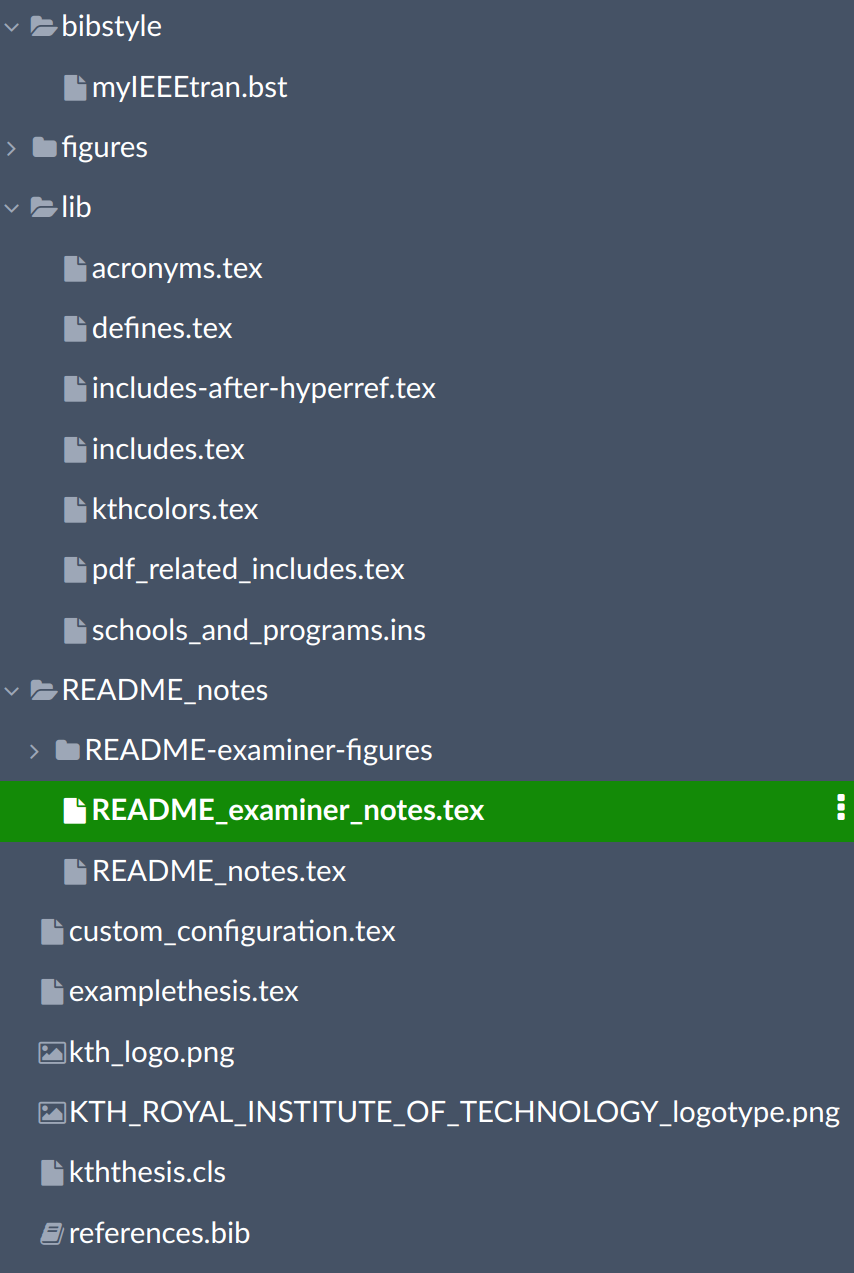
\includegraphics[width=0.5\textwidth]{README_notes/README-examiner-figures/Overleaf_folders_and_files_Screenshot_20220330_150822.png}}
  \end{center}
  \caption{Files and folders in Overleaf template}
  \label{fig:overleafFoldersAndFiles}
\end{figure}
\FloatBarrier

There are currently instructions concerning the template in 
\iflabelexists{ch:READMEnotes}{\Cref{ch:READMEnotes}.}
{xxxx- You have to include the \texttt{README\_notes/README\_notes.tex} file when compiling to get additional information.}
Ideally, these instructions should be available in both English and Swedish; however, a Swedish version remains as future work.

Most students will only need to add acronyms to the \texttt{acronyms.tex} file and perhaps additional packages to \texttt{includes.text} (in some cases these may need to be added to the \texttt{includes-after-hyperref.tex} file if there is a conflict with \texttt{hyperref}).

The \texttt{schools\_and\_programs.ins} and \texttt{old\_schools\_and\_programs.ins} were generated from the data in KOPPS. Students will not have to change these files.
%The \texttt{old\_schools\_and\_programs.ins} file has now been removed from the template.
\clearpage


\section{Generating LaTeX commands for in the student’s thesis source file}
The thesis makes use of a set of \LaTeX~commands to collect information about the student, the supervisor(s), and the examiner. However, how can a student know what their KTHID and other necessary information is?

There are two alternatives:
\begin{itemize}
    \item The examiner or someone can use the method described in \Cref{sec:makeItSimpleFromTheStart} or

    \item They can make use of the program: \texttt{whoami\_for\_latex.py}\footnote{Note that this program requires access to LADOK; hence, it is \textbf{no longer available}. However, a version that does not need LADOK access could be used by a student to get their own information from Canvas, \textit{excluding their program information}; as Canvas does not currently have any source for the student's program information.}.
    
    The \texttt{whoami\_for\_latex.py} program makes use of information from the Canvas course room where the student is enrolled for their degree project. In the examples below we will assume that this is the Canvas course\_id 25434.
\end{itemize}

\Cref{lst:whoami2} shows the case for a student author who has the e-mail address “oscarros@kth.se”. Note that the user is prompted to enter their KTH account name and password (in order to access LADOK). Note that this student has two programs of study listed in LADOK (\ie CDATE and TCSCM). The student will have to manually select one of these and comment out or delete the other. The course code is derived from the section of the course that the user is enrolled in. This section name (in the case of this student: “DA231XVT212”) is reduced to a course code by truncation. The course cycle information is taken from the first digit of the course code. This should work for most course codes, except for one program in architecture which is still using a very old course code.
\Needspace*{28\baselineskip}
\begin{lstlisting}[language={bash}, caption={Generating \LaTeX~commands for a student author}, label=lst:whoami]
./whoami_for_latex.py oscarxxxxxs@kth.se 25434
login_id=oscarxxxxxs@kth.se
\authorsLastname{xxxxxx}
\authorsFirstname{Oscar}
\email{oscarros@kth.se}
\kthid{u1xxxxx}
%\authorsSchool{\schoolAcronym{XXX}}
\programcode{CDATE}
% Note that the following line should be commented out, as the programme is derived from the school_and_Programs.ins information
%\programname{Degree Programme in XXX}
\programcode{TXXXX}
% Note that the following line should be commented out, as the programme is derived from the school_and_Programs.ins information
%\programname{Master's Programme, XXX}
\courseCycle{2}
\courseCode{DA231X}
\end{lstlisting}

\Cref{lst:whoami2} show the case of generating the data for a second author (\textbf{NB} this is only possible for a first-cycle thesis). The actual user data has been anonymized in this figure.
\Needspace*{24\baselineskip}
\begin{lstlisting}[language={bash}, caption={Generating the \LaTeX~data for the second author (in the case of a first-cycle thesis)}, label=lst:whoami2]
./whoami_for_latex.py -2 xxxx@kth.se 22156
\secondAuthorsLastname{xxxxx}
\secondAuthorsFirstname{xxxxx}
\secondemail{xxxx@kth.se}
\secondkthid{u1xxxxx}
\secondAuthorsSchool{\schoolAcronym{XXX}}
%Note that the LaTeX template does not support having students with different programs or course codes
\programcode{CINTE}
% Note that the following line should be commented out, as the programme is derived from the school_and_Programs.ins information
%\programname{Degree Programme in Information and Communication Technology}
\courseCycle{1}
\courseCode{IA150X}
\end{lstlisting}


\Cref{lst:secondAuthor} shows the case where the program has been run to add a second author to a second-cycle thesis, note the warning message in the last line of this figure.

\begin{lstlisting}[language={bash}, caption={Attempting to generate a 2\textsuperscript{nd} author for a second-cycle thesis}, label=lst:secondAuthor]
./whoami_for_latex.py -2 oscarros@kth.se 25434
\secondAuthorsLastname{Rosquis}
\secondAuthorsFirstname{Oscar}
\secondemail{oscarros@kth.se}
\secondkthid{u1tmg8l6}
\secondAuthorsSchool{\schoolAcronym{XXX}}
%Note that the LaTeX template does not support having students with different programs or course codes
\programcode{CDATE}
% Note that the following line should be commented out, as the programme is derived from the \texttt{school_and\_Programs.ins} information
%\programname{Degree Programme in XXX}
\courseCycle{2}
\courseCode{XX200X}
latex_courseCycle=\courseCycle{2}, type=<class 'str'>
%%%% Note that a second-cycle thesis should not have two authors!!!
\programcode{TCSCM}
% Note that the following line should be commented out, as the programme is derived from the \texttt{school_and\_Programs.ins} information
%\programname{Master's Programme, XXX}
\courseCycle{2}
\courseCode{XX200X}
latex_courseCycle=\courseCycle{2}, type=<class 'str'>
%%%% Note that a 2nd cycle thesis should not have two authors!!!
\end{lstlisting}

\Cref{lst:supervisor} shows the case for a supervisor who has the e-mail address “vastberg@kth.se”.  \Cref{lst:examiner} shows the case for an examiner who has the e-mail address “maguire@kth.se”.  Note that the information about the school and department (in the case of a supervisor and examiner) are currently fixed and commented out – so that the user can edit them as necessary.
\Needspace*{10\baselineskip}
\begin{lstlisting}[language={bash}, caption={Generating \LaTeX~commands for a supervisor}, label=lst:supervisor]
./whoami_for_latex.py vastberg@kth.se 25434
%If not the first supervisor, then replace supervisorAs with supervisorBs or supervisorCs as appropriate
\supervisorAsLastname{Västber}
\supervisorAsFirstname{Anders}
\supervisorAsEmail{vastberg@kth.se}
% If the supervisor is from within KTH add their KTHID, School and Department info
%\supervisorAsSchool{\schoolAcronym{XXX}}
%\supervisorAsDepartment{DepartmentName}
\end{lstlisting}
\Needspace*{8\baselineskip}
\begin{lstlisting}[language={bash}, caption={Generating \LaTeX~commands for the examiner}, label=lst:examiner]
./whoami_for_latex.py -e xxx@kth.se 25434
\examinersLastname{ExaminersLastname}
\examinersFirstname{ExaminersFirstname}
\examinersEmail{xxx@kth.se}
% If the examiner is from within KTH add their KTHID, School and Department info
\examinersSchool{\schoolAcronym{XXX}}
\examinersDepartment{DepartmentName}
\end{lstlisting}
 	
The program: whoam\_for\_latex.py is far more powerful that shown in the examples above, it can take other identifiers for the user in instead of an e-mail address, such as a Canvas user\_id or a KTHID. Additionally, rather than specifying the Canvas course room’s course\_id, it is also possible to use the name of the course room and even a nickname (if you have defined a nickname in your Canvas dashboard). See the README file in \url{https://gits-15.sys.kth.se/maguire/ladok3}.


\section{Alternative way of inserting the covers}
Another way that the covers can be inserted is to use the \textsc{pdfpages} package (as shown in \Cref{lst:includeAfterHyperref}), then insert the two cover pages at the appropriate place (as shown in \Cref{lst:frontCover} and \Cref{lst:backCover}). This assumes that you have made the covers using some other method and now want to insert them into the Overleaf project. Unfortunately, I do not yet know how I can programmatically insert these two files into the Overleaf project (presumably into a folder “covers”). Here we assume that the user has manually uploaded the two files into the covers folder.
\Needspace*{6\baselineskip}
\begin{lstlisting}[language={[LaTeX]TeX}, caption={Insert this include file either in the main text document or the includes.tex file}, label=lst:includeAfterHyperref]
% To use KTH pdf covers
\usepackage{pdfpages}

% packages that have to be included after hyperref
\usepackage{doi}
\usepackage{cleveref}           %% Replace Section with a symbol
\usepackage{hyperxmp}           %% to be able to add the copyright information to the PDF metadata

% To be able to attach files to the final PDF
% Note that the package used is attachfile2 and not attachfile - as the former supports most TeX engines
\usepackage{attachfile2}

%% If you are going to set bidirectional text, i.e., left to right and right to left, add bidi as the last package
%\usepackage{bidi}

\end{lstlisting} 	
\Needspace*{6\baselineskip}
\begin{lstlisting}[language={[LaTeX]TeX}, caption={Insert the front cover before the title page}, label=lst:frontCover]
% Add front cover
\includepdf[pages=-]{covers/front.pdf}

%%% Set the numbering for the title page to a numbering series not in the preface or body
\pagenumbering{alph}
\end{lstlisting}

\Needspace*{5\baselineskip}
\begin{lstlisting}[language={[LaTeX]TeX}, caption={Insert the back cover page before the For DiVA section}, label=lst:backCover]
% Add back cover, unsure if this is supposed to be before or after the "For DiVA" pages
\includepdf[pages=-]{covers/back.pdf}

\section*{For DIVA}
\end{lstlisting}

Note that the name of the section should actually include four euro symbols and a space before the "For DIVA" and a space and 4 euro symbols after it. This is necessary to have this Appendix in the thesis. If you do not have this appendix, then you can use the name of the section as shown above.
\clearpage

\section{The big picture}

\Cref{tab:inforAndItsUses} shows the relationship between the information and the programs that use it. The sections highlighted in yellow are optional. For example, only first-cycle theses will have a second author. While all theses will have one supervisor, some may have more (the programs support up to 10). The assumption is that there is a single examiner, but there is the ability to add more (this also requires modifying the programs that use this information). Not every project involves external cooperation – note also that while the MODS program writes out this information the DiVA import does not import this information.

Individuals can be associated with KTH, in this case, they have a Local User Id and an organization element (with the implicit top level (L0) being KTH)). The organization levels of L1 == School and L2 == Department. It is possible to extend this further, but the programs currently only support L1 and L2. The Title and Alternative title fields are used to support the English and Swedish title (or visa versa) -– similarly, the abstracts and keywords must include English and Swedish – versions with support for abstracts and keywords in many languages. Note that Credits must be given to one decimal place.
Note that it would be very rare that the examiner is from outside of KTH, but this should (probably) be supported. Where a school should be specified one can use \textbackslash schoolAcronym\{xxx\}.

The Canvas course room’s course\_id is often an argument to the programs. One reason for this is to publish the announcement in the correct course room and calendar. Another reason for this is to be able to use the information in the course room to translate a local user ID (\ie a kthid) to an integration ID (\ie a LADOK user ID) or to be able to look up details of an author, examiner, or supervisor.



\begin{landscape}
\small{
\begin{longtable}{L{2cm}|L{4cm}|l|L{4cm}|L{4cm}|l l l l|}
\caption{Information and how it is used}\label{tab:inforAndItsUses}\\
    &  & & & \textbf{DOCX DocProperty} &  &  &  & \\
    \textbf{Top level} & \textbf{elements} & \textbf{subelements}	& \textbf{\LaTeX~Macro} & \textbf{or fields} & \begin{rotate}{60}\textbf{calendar}\end{rotate} & \begin{rotate}{60}\textbf{cover}\end{rotate} & \begin{rotate}{60} \textbf{LADOK}\end{rotate} & \begin{rotate}{60}\textbf{MODS}\end{rotate}\\
        \endfirsthead
    \multicolumn{9}{c}%
{\tablename\ \thetable\ -- \textit{Continued from previous page}} \\
    &  &	&  & \textbf{DOCX DocProperty} &  &  &  & \\
    \textbf{Top level} & \textbf{elements} & \textbf{subelements}	& \textbf{\LaTeX~Macro} & \textbf{or fields} & \begin{rotate}{60}\textbf{calendar}\end{rotate} & \begin{rotate}{60}\textbf{cover}\end{rotate} & \begin{rotate}{60} \textbf{LADOK}\end{rotate} & \begin{rotate}{60}\textbf{MODS}\end{rotate}\\
\hline
\endhead
      \hline
Author1	\\
&	Last name &	&	\textbackslash authorsLastname\{\} &	Author1\_Last\_name & x &	x &	x &	x\\
&	First name & &	\textbackslash authorsFirstname\{\} &	Author1\_First\_name & x & x & x & x\\
&	Local User Id &	& \textbackslash kthid\{\} &	Author1\_Local User Id &	& 		& x &	x \\
&	E-mail	& &	\textbackslash email\{\} &	Author1\_E-mail	&	& & &		x \\
 & organisation & \\
 &  & L1 & \textbackslash authorsSchool\{\} & Author1\_organization\_L1 &  &  &  & x\\
 &  &  &  & Author1\_organization\_L2 &  &  &  & \\
 & Other organisation &  &  & Author1\_Other\_organisation &  &  &  & \\
       \hline
\rowcolor{yellow}Author2 & \multicolumn{8}{l}{\cellcolor{yellow}}\\
\rowcolor{yellow} & Last name &  & \textbackslash secondAuthorsLastname\{\} & Author2\_Last\_name & x & x & x & x\\
\rowcolor{yellow} & First name &  & \textbackslash secondAuthorsFirstname\{\} & Author2\_First\_name & x & x & x & x\\
\rowcolor{yellow} & Local User Id &  & \textbackslash secondkthid\{\} & Author2\_Local User Id &  &  & x & x\\
\rowcolor{yellow} & E-mail &  & \textbackslash secondemail\{\} & Author2\_E-mail &  &  &  & x\\
\rowcolor{yellow} & organisation & \multicolumn{7}{l}{\cellcolor{yellow}}\\ 
\rowcolor{yellow} &  & L1 & \textbackslash secondAuthorsSchool{ } & Author2\_organization\_L1 &  &  &  & x\\
\rowcolor{yellow} &  &  &  & Author2\_organization\_L2 &  &  &  & \\
\rowcolor{yellow} & Other organisation &  &  & Author2\_Other\_organisation &  &  &  & \\
       \hline
Cycle &  &  & \textbackslash courseCycle\{\} & Cycle & x & x &  & \\
Course code &  &  & \textbackslash courseCode\{\} & Course\_code & i & i &  &  \\
Credits &  &  & \textbackslash courseCredits\{\} & Credits &  &  &  & \\
      \hline
Degree1 & \\
 & Educational program &  & Derived from programcode & Educational program &  & x &  & x \\
 & programcode &  & \textbackslash programcode\{\} & programcode &  & i &  & i \\
 & Degree &  & \textbackslash degreeName\{\} & Degree &  & x &  & x \\
 & subjectArea &  & \textbackslash subjectArea{ } & subjectArea &  & x &  & x \\
\rowcolor{yellow}Degree2 & \multicolumn{8}{l}{\cellcolor{yellow}}\\
\rowcolor{yellow}& Educational program &  & Derived from secondProgramcode & second\_Educational program &  & x &  & x \\
\rowcolor{yellow}& programcode &  & \textbackslash secondProgramcode\{\} & second\_Programcode &  & i &  & i \\
\rowcolor{yellow}& Degree &  & \textbackslash secondDegreeName\{\} & second\_Degree &  & x &  & x \\
\rowcolor{yellow}& subjectArea &  & \textbackslash secondSubjectArea\{\} & second\_subjectArea &  & x &  & x \\
       \hline
Title & \\
 & Main title &  & \textbackslash title\{\} & (exiting document property) & x & x & x & x \\
 & Subtitle &  & \textbackslash subtitle\{\} & Subtitle & x & x & o & x \\
 & Language &  & Derived from option to document class &  & x &  &  & x \\
Alternative title & \\
 & Main title &  & \textbackslash alttitle\{\} & Alternative\_main\_title & x & x & x & x \\
 & Subtitle &  & \textbackslash altsubtitle\{\} & Alternative\_subtitle & x & x & o & x \\
 & Language &  & Derived from option to documentclass &  & x &  &  & x \\
      \hline
Supervisor1 & \\
 & Last name &  & \textbackslash supervisorAsLastname\{\} & Supervisor1\_Last\_name & x &  &  & x \\
 & First name &  & \textbackslash supervisorAsFirstname\{\} & Supervisor1\_First\_name & x &  &  & x \\
 & Local User Id &  & \textbackslash supervisorAsKTHID\{\} & Supervisor1\_Local User Id &  &  &  & x \\
 & E-mail &  & \textbackslash supervisorAsEmail\{\} & Supervisor1\_E-mail &  &  &  & x \\
 & organisation & \\
 &  & L1 & \textbackslash supervisorAsSchool\{\} & Supervisor1\_organization\_L1 &  &  &  & x \\
 &  & L2 & supervisorAsDepartment\{\} & Supervisor1\_organization\_L2 &  &  &  & o \\
 & Other organisation &  & supervisorAsOrganization\{\} & Supervisor1\_Other\_organisation &  &  &  &  \\
\rowcolor{yellow}Supervisor2 &  \multicolumn{8}{l}{\cellcolor{yellow}}\\
\rowcolor{yellow} & Last name &  & \textbackslash supervisorBsLastname{ } & Supervisor2\_Last\_name & x &  &  & x \\
\rowcolor{yellow} & First name &  & \textbackslash supervisorBsFirstname\{\} & Supervisor2\_First\_name & x &  &  & x \\
\rowcolor{yellow} & Local User Id &  & \textbackslash supervisorBsKTHID\{\} & Supervisor2\_Local User Id &  &  &  & x \\
\rowcolor{yellow} & E-mail &  & \textbackslash supervisorBsEmail\{\} & Supervisor2\_E-mail &  &  &  & x \\
\rowcolor{yellow} & organisation & \multicolumn{7}{l}{\cellcolor{yellow}}\\
\rowcolor{yellow} &  & L1 & \textbackslash supervisorBsSchool\{\} & Supervisor2\_organization\_L1 &  &  &  & x \\
\rowcolor{yellow} &  & L2 & \textbackslash supervisorBsDepartment\{\} & Supervisor2\_organization\_L2 &  &  &  & o \\
\rowcolor{yellow} & Other organisation &  & \textbackslash supervisorBsOrganization\{\} & Supervisor2\_Other\_organisation &  &  &  & \\
\rowcolor{yellow}Supervisor3 & \multicolumn{8}{l}{\cellcolor{yellow}} \\
\rowcolor{yellow} & Last name &  & \textbackslash supervisorCsLastname\{\} & Supervisor3\_Last\_name & x &  &  & x \\
\rowcolor{yellow} & First name &  & \textbackslash supervisorCsFirstname\{\} & Supervisor3\_First\_name & x &  &  & x \\
\rowcolor{yellow} & Local User Id &  & \textbackslash supervisorCsKTHID\{\} &  &  &  &  & \\ 
\rowcolor{yellow} & E-mail &  & \textbackslash supervisorCsEmail\{\} & Supervisor3\_E-mail &  &  &  & o \\
\rowcolor{yellow} & organisation & \multicolumn{7}{l}{\cellcolor{yellow}}\\ 
\rowcolor{yellow} &  & L1 & \textbackslash supervisorCsSchool\{\} & Supervisor3\_organization\_L1 &  &  &  & x \\
\rowcolor{yellow} &  & L2 & \textbackslash supervisorCsDepartment\{\} & Supervisor3\_organization\_L2 &  &  &  & o \\
\rowcolor{yellow} & Other organisation &  & \textbackslash supervisorCsOrganization\{\} & Supervisor3\_Other\_organisation & x &  &  &  x \\
Examiner1 & \\
 & Last name &  & \textbackslash examinersLastname\{\} & Examiner1\_Last\_name & x &  & i & x \\
 & First name &  & \textbackslash examinersFirstname\{\} & Examiner1\_First\_name & x &  & i & x \\
 & Local User Id &  & \textbackslash examinersKTHID\{\} & Examiner1\_Local User Id &  &  & i & x \\
 & E-mail &  & \textbackslash examinersEmail\{\} & Examiner1\_E-mail &  &  &  & x \\
 & organisation & \\
 &  & L1 & \textbackslash examinersSchool\{\} & Examiner1\_organization\_L1 &  &  &  & x \\
 &  & L2 & \textbackslash examinersDepartment\{\} & Examiner1\_organization\_L2 &  &  &  & \\
 & Other organisation &  & \textbackslash examinersOrganization\{\} &  &  &  &  & o \\
 \hline
\rowcolor{yellow}Cooperation & \multicolumn{8}{l}{\cellcolor{yellow}}\\
\rowcolor{yellow} & Partner\_name &  & \textbackslash hostcompany\{\}        or \textbackslash hostorganization\{\} & Cooperation\_Partner\_name &  &  &  & o \\
  \hline
National Subject Categories &  &  & \textbackslash nationalsubjectcategories\{\} & National Subject Categories &  &  &  & x \\
 \hline
Other information & \\
 & Year &  & \textbackslash the\textbackslash year & (derived from document property Date) &  &  &  & x \\
 & Number of pages &  & (derived from labels: pg:lastPageofPreface and pg:lastPageofMainmatter) & (derived from bookmarks: lastPageofPreface and lastPageofMainmatter) &  &  &  & x \\
Series & \\
 & Title of series &  & \textbackslash trita{TRITA-XXX-EX}{2021:00} & Series\_name &  & x &  & x \\
 & No. in series &  &  & Number\_in\_series &  & x &  & x \\
Opponents &  &  & \textbackslash opponentsNames\{\} & Opponents\_Name & x &  &  & \\
Presentation & \\
 & Date &  & \textbackslash presentationDateAndTimeISO\{\} & Presentation\_Date & x &  &  & x \\
 & Language &  & \textbackslash presentationLanguage{ } & Presentation\_Language & x &  &  & x \\
 & Room &  & \textbackslash presentationRoom\{\} & Presentation\_Room & x &  &  & x \\
 & Address &  & \textbackslash presentationAddress{ } & Presentation\_Address & x &  &  & x \\
 & City &  & \textbackslash presentationCity{ } & Presentation\_City & x &  &  & x \\
\hline
Number of lang instances &  &  &  & [Manually entered as 2, 3, 4, …] &  &  &  & \\
abstracts & \\
 & eng &  & (saved in lang array using scontents) & (derived from bookmark: EnglishAbstract and then text inserted) & x &  &  & x \\
 & swe &  &  & (derived from bookmark: SwedishAbstract) & x &  &  & x \\
 & \cellcolor{yellow}fre &\cellcolor{yellow}  & & \multicolumn{4}{l}{\cellcolor{yellow}} & \cellcolor{yellow}o\\
 & \cellcolor{yellow}… & \cellcolor{yellow} & & \multicolumn{4}{l}{\cellcolor{yellow}} & \cellcolor{yellow}o\\
keywords & \\
 & eng &  & (saved in lang array using scontents) & (derived from bookmark: EnglishKeywords) & x &  &  & x \\
 & swe &  &  & (derived from bookmark: SwedishKeywords) & x &  &  & x \\
 & \cellcolor{yellow}fre & \cellcolor{yellow} & & \multicolumn{4}{l}{\cellcolor{yellow}} & \cellcolor{yellow}o \\
 & \cellcolor{yellow}… & \cellcolor{yellow} & & \multicolumn{4}{l}{\cellcolor{yellow}} & \cellcolor{yellow}o\\
\hline
\end{longtable}
}
\end{landscape}

\section{Alternative way of generating JSON for a \LaTeX~template}
\label{sec:AlternativeWayofGeneratingJSON}
After writing a program to extract the JSON information directly from the DOCX file, I was inspired to try to more directly get the JASON data from the \LaTeX~template; thus, in both cases avoiding the need to parse the PDF file.
While one might think about simply writing the information to a file rather than rendering it in the PDF document, there turned out to be several problems, as the \LaTeX\ \textbackslash write turns out not to expand commands that are not expandable – while writing this same content to the page ends up with the correct rendering of the page (as this action causes the expansion and evaluation of the commands).

The first problem that I encountered was that the \texttt{xstring} function \textbackslash IfEqCase that I had used in a number of places turned out to not be expandable in a \textbackslash immediate \textbackslash write call. Thus I needed to use an expandable version. The new code for \texttt{kththesis.cls} is shown in \Cref{lst:InsertKeywords}. I changed to use \texttt{expl3 strcompare} rather than xstring's \texttt{IfEqCase}, since the later is not expandable . For example, the original school acronym code needed to be replaced by the code in \Cref{lst:newSchoolAcronym}. Similarly, for the code of \textbackslash programmecode (partially) shown in 
\Cref{lst:newProgramcode}. The fake school code of XXX and fake program codes (TXXXX and CXXXX) were manually introduced for use in this template on 2025-06-12.
\begin{comment}
    This means that there needed to be a new schools\_and\_programs.ins file. \textbf{As of 2022-12-19, there is a new program \texttt{get-school-acronyms-and-program-names-data.py} to generate this file from KOPPS data access via the KOPPS API. Note that this program also generates data about the course codes with the name of the course in English and Swedish.}
\end{comment}
\warningExpl{As of 2025-06-01, the KOPPS API has been shutdown, so it is no longer possible to programmatically generate this file.}

\Needspace*{11\baselineskip}
\begin{lstlisting}[language={[LaTeX]TeX}, caption={New version of \textbackslash InsertKeywords together with making the expl3 \textbackslash strcompare function available}, label=lst:InsertKeywords]
\ExplSyntaxOn
\cs_new_eq:NN \strcompare \str_if_eq:nnTF
\ExplSyntaxOff

\newcommand{\InsertKeywords}[1]{
\strcompare{#1}{english}{\@EnglishKeywords}{}%
\strcompare{#1}{swedish}{\@SwedishKeywords}{}%
}
\end{lstlisting}

\Needspace*{28\baselineskip}
\begin{lstlisting}[language={[LaTeX]TeX}, caption={New \textbackslash schoolAcronym}, label=lst:newSchoolAcronym] 
% The strcompare is added to kththesis.cls
\newcommand{\schoolAcronym}[1]{%
  \ifinswedish
    \strcompare{#1}{ABE}{Skolan för Arkitektur och samhällsbyggnad}{}%
    \strcompare{#1}{ITM}{Skolan för Industriell teknik och management}{}%
    \strcompare{#1}{SCI}{Skolan för Teknikvetenskap}{}%
    \strcompare{#1}{CBH}{Skolan för Kemi, bioteknologi och hälsa}{}%
    \strcompare{#1}{EECS}{Skolan för Elektroteknik och datavetenskap}{}%
    \strcompare{#1}{XXX}{*****Skolan för XXX*****}{}% Fake school for use in template
  \else
    \strcompare{#1}{ABE}{School of Architecture and the Built Environment}{}%
    \strcompare{#1}{ITM}{School of Industrial Engineering and Management}{}%
    \strcompare{#1}{SCI}{School of Engineering Sciences}{}%
    \strcompare{#1}{CBH}{School of Engineering Sciences in Chemistry, Biotechnology and Health}{}%
    \strcompare{#1}{EECS}{School of Electrical Engineering and Computer Science}{}%
    \strcompare{#1}{XXX}{*****School of XXX*****}{}% Fake school for use in template
  \fi
}
\end{lstlisting}
	
\Needspace*{20\baselineskip}
\begin{lstlisting}[language={[LaTeX]TeX}, caption={New version of \textbackslash programcode}, label=lst:newProgramcode] 
\newcommand{\programmecode}[1]{%
  \ifinswedish
    \strcompare{#1}{ARKIT}{Arkitektutbildning}{}%
    \strcompare{#1}{CBIOT}{Civilingenjörsutbildning i bioteknik}{}%
...
\strcompare{#1}{TURSM}{Magisterprogram, urbana studier}{}%
  \else
    \strcompare{#1}{ARKIT}{Degree Programme in Architecture}{}%
    \strcompare{#1}{CBIOT}{Degree Programme in Biotechnology}{}%
 ...
   \strcompare{#1}{TURSM}{Master's Programme, Urbanism Studies, 60 credits}{}%
  \fi
}
\end{lstlisting}
\Needspace*{30\baselineskip}
\Cref{lst:codeToWriteToJSONfile} shows the code to write the first author’s information to the JSON file.
\begin{lstlisting}[language={[LaTeX]TeX}, caption={Code to write the first author's information to a "JSON" file}, label=lst:codeToWriteToJSONfile] 
\newwrite\jsonfile
    \immediate\openout\jsonfile=fordiva.json
    \immediate\write\jsonfile{ \@charlb }
    \immediate\write\jsonfile{"Author1": \@charlb \ifx\@authorsLastname\@empty%\relax
     \else
     "Last name": "\@authorsLastname",
     \fi
     \ifx\@authorsFirstname\@empty%\relax
     \else
     "First name": "\@authorsFirstname",
     \fi
     \ifx\@kthid\@empty%\relax
     \else
     "Local User Id": "\@kthid",
     \fi
     \ifx\@email\@empty%\relax
     \else
     "E-mail": "\@email",
     \fi
     \ifx\@authorsSchool\@empty%\relax
     \else
     "organisation": \@charlb"L1": "\@authorsSchool"
     \ifx\@authorsDepartment\@empty%\relax
     \else
     ,"L2": "\@authorsDepartment"
     \fi
     \@charrb
     \fi
    \@charrb,}
…
\immediate\write\jsonfile{\@charrb} % end the JSON dict
\closeout\jsonfile
\end{lstlisting}

The second problem that I encountered was that the function \texttt{\textbackslash pageref} used to get the page numbers of the end of the preface and the last page of the document were also not expandable. This was solved using the package \texttt{refcount} to be able to get an expandable \texttt{\textbackslash getpagerefnumber}. This new code is shown in \Cref{lst:newCodeToOutputPageNumbers}.
\Needspace*{12\baselineskip}
\begin{lstlisting}[language={[LaTeX]TeX}, caption={New code to output the "Other information" including page numbers}, label=lst:newCodeToOutputPageNumbers]
    % "\pageref{pg:lastPageofPreface},\pageref{pg:lastPageofMainmatter}" \@charrb,
    \immediate\write\jsonfile{
    "Other information": \@charlb"Year": "\the\year", "Number of pages": 
    "\getpagerefnumber{pg:lastPageofPreface},\getpagerefnumber{pg:lastPageofMainmatter}" \@charrb,
    }
\end{lstlisting}

The third problem turned out to be much harder to solve. The \textsc{scontents} related functions that I used in the newcommand \texttt{\textbackslash divainfo}: \textbackslash getstored[\textbackslash i]{lang}, \textbackslash getstored[\textbackslash i]\{keywords\}, and \textbackslash typestoredx{\textbackslash i}\{abstracts\} also turned out to not be expandable. The approach taken here is somewhat of a cheat in that it required getting the strings directly from the \textsc{scontents} buffer (see the code in \Cref{lst:functionToGetscontents}) and then using xstring’s \texttt{tokenize}  function (see the code in \Cref{lst:functionToGetscontents}).
\Needspace*{8\baselineskip}
\begin{lstlisting}[language={[LaTeX]TeX}, caption={Function to get the scontents}, label=lst:functionToGetscontents]
\ExplSyntaxOn
% Note that this function returns the _string_ stored in the scontents buffer
\cs_new:Npn \qgetstored #1 #2
{
\__scontents_getfrom_seq:nn {#1} {#2}
}
\end{lstlisting}
	
\Needspace*{28\baselineskip}
\begin{lstlisting}[language={[LaTeX]TeX}, caption={Writing out the language, abstract, and keywords information}, label=lst:writinglangAndKeywords]
\immediate\write\jsonfile{"Number of lang instances": "\countsc{lang}",}

\immediate\write\jsonfile{"abstracts": \@charlb}
 \foreach \i in {1,...,\countsc{lang}} {
 %\getstored[\i]{lang}
  \newcommand{\templangs}{\qgetstored{\i}{lang}}
  \tokenize{\lang}{\templangs}
  \immediate\write\jsonfile{"\lang": "\qgetstored{\i}{abstracts}"}
  \immediate\write\jsonfile{,}
}
\immediate\write\jsonfile{\@charrb} % end the abstracts dict


\immediate\write\jsonfile{"keywords": \@charlb}
 \foreach \i in {1,...,\countsc{lang}} {
    \newcommand{\templangs}{\qgetstored{\i}{lang}}
    \tokenize{\lang}{\templangs}
    \newcommand{\fee}{\qgetstored{\i}{keywords}}
    % Because \qgetstored{\i}{keywords} returned a string,
    % we need to convert this string into tokens so it can be evaluate
    % we do this using the function \tokenisze from the xstring package
    \tokenize{\fumble}{\fee}
    \immediate\write\jsonfile{"\lang": "\fumble"}

    \immediate\write\jsonfile{,}
}
    \immediate\write\jsonfile{\@charrb} % end the keywords dict
\end{lstlisting}	


The result is that \LaTeX~directly generates a file named “\texttt{fordiva.json}” with the (almost) desired information in it. See \Cref{lst:resultingForDIVAfile} for an example of such a file. As of 2025-05-03, the contents of the \texttt{fordiva.json} file are attached to the last page of the printed data. This means that it can be directly extracted!

	
\begin{lstlisting}[language={json}, caption={Resulting fordiva.json file}, label=lst:resultingForDIVAfile]
{
"Author1": {"Last name": "Student", "First name": "Fake A.", "Local User Id": "u100001", "E-mail": "a@kth.se", "organisation": {"L1": "School of XXX" }},
"Author2": {"Last name": "Student", "First name": "Fake B.", "Local User Id": "u100002", "E-mail": "b@kth.se", "organisation": {"L1": "School of XXX" }},
"Cycle": "1", "Course code": "XX100X", "Credits": "15.0", 
"Degree1": {"Educational program": "" ,"programcode": "TCOMK" ,"Degree": "Bachelors degree" ,"subjectArea": "Information and Communication Technology" }, 
"Title": {"Main title": "This is the title in the language of the thesis", "Subtitle": "An subtitle in the language of the thesis", "Language": "eng" }, "Alternative title": {"Main title": "Detta är den svenska översättningen av titeln", "Subtitle": "Detta är den svenska översättningen av undertiteln", "Language": "swe" }, 
"Supervisor1": {"Last name": "Supervisor", "First name": "A. Busy", "Local User Id": "u100003", "E-mail": "sa@kth.se", "organisation": {"L1": "School of XXX" ,"L2": "DepartmentName" }}, 
"Supervisor2": {"Last name": "Supervisor", "First name": "Another Busy", "Local User Id": "u100003", "E-mail": "sb@kth.se", "organisation": {"L1": "School of XXX" ,"L2": "DepartmentName" }}, 
"Supervisor3": {"Last name": "Supervisor", "First name": "Third Busy", "E-mail": "sc@tu.va", "Other organisation": "Timbuktu University, Department of Pseudoscience" }, 
"Examiner1": {"Last name": "ExaminersLastname", "First name": "ExaminersFirstname", "Local User Id": "u1000000", "E-mail": "xxx@kth.se", "organisation": {"L1": "School of XXX" ,"L2": "DepartmentName" }}, 
"Cooperation": {"Partner_name": "Företaget AB"}, 
"National Subject Categories": "10201, 10206", 
"Other information": {"Year": "2021", "Number of pages": "xxxv,35" }, 
"Series": {"Title of series": "TRITA-XXX-EX" , "No. in series": "2021:00" }, 
"Opponents": {"Name": "A. B. Normal \& A. X. E. Normalè"}, 
"Presentation": {"Date": "2021-03-15 13:00" ,"Language": "eng" ,"Room": "via Zoom https://kth-se.zoom.us/j/ddddddddddd" ,"Address": "Isafjordsgatan 22 (Kistagången 16)" ,"City": "Stockholm" }, 
"Number of lang instances": "10",
"abstracts": {
"eng": €€€€
"Write an abstract that is about \textit{250 and 350 words} (1/2 A4-page)  with the following components: % key parts of the abstract
\begin{itemize}
  \item What is the topic area? (optional) Introduces the subject area for the project.
  \item Short problem statement
  \item Why was this problem worth a Bachelor's/Master’s thesis project? (\ie, why is the problem both significant and of a suitable degree of difficulty for a Bachelor's/Master’s thesis project? Why has no one else solved it yet?)
  \item How did you solve the problem? What was your method/insight?
  \item Results/Conclusions/Consequences/Impact: What are your key results/\linebreak[4]conclusions? What will others do based upon your results? What can be done now that you have finished - that could not be done before your thesis project was completed?
\end{itemize}

For testing the following lines were added.
Choice of typeface with \textbackslash textit, \textbackslash textbf, and \textbackslash texttt:  \textit{x}, \textbf{x}, and \texttt{x}

Text superscripts and subscripts with \textbackslash textsubscript and \textbackslash textsuperscript: A\textsubscript{x} and A\textsuperscript{x}

Some useful symbols: \textbackslash textregistered, \textbackslash texttrademark, and \textbackslash textcopyright. For example, copyright symbol: \textbackslash textcopyright Maguire 2021, and some superscripts: \textbackslash textsuperscript\{99m\}Tc, A\textbackslash textsuperscript\{*\}, A\textbackslash textsuperscript\{\textbackslash textregistered\}, and A\textbackslash texttrademark : \textcopyright Maguire 2021, and some superscripts: \textsuperscript{99m}Tc, A\textsuperscript{*}, A\textsuperscript{\textregistered}, and A\texttrademark. Another example: H\textbackslash textsubscript\{2\}O: H\textsubscript{2}O

\begin{enumerate}
  \item The first item is a simple \textbf{strong} statement
  \item The second item is a simple statement
  \item The third item is an \textit{italicized} statement
\end{enumerate}

Yet more text can be added.

The following commands can be used: \textbackslash eg, \textbackslash Eg, \textbackslash ie, \textbackslash Ie, \textbackslash etc, and \textbackslash etal: \eg, \Eg, \ie, \Ie, \etc, and \etal

The following commands for numbering with lower case roman numerals: \textbackslash first, \textbackslash Second, \textbackslash third, \textbackslash fourth, \textbackslash fifth, \textbackslash sixth, \textbackslash seventh, and \textbackslash eighth: \first, \Second, \third, \fourth, \fifth, \sixth, \seventh, and \eighth.

Equations using \textbackslash( xxxx \textbackslash) or \textbackslash[ xxxx \textbackslash] can be used in the abstract. For example: \( (C_5O_2H_8)_n \)
or \[ \int_{a}^{b} x^2 \,dx \]

The above showed even more text and equations.
"
€€€€,
"swe": €€€€
"Denna avhandling undersöker problemet  \ldots"
€€€€,
"fre": €€€€
"Résumé en français."
€€€€,
"spa": €€€€
"Résumé en espagnol."
€€€€,
"ita": €€€€
"Sommario in italiano."
€€€€,
"nor": €€€€
"Sammendrag på norsk."
€€€€,
"ger": €€€€
"Zusammenfassung in Deutsch."
€€€€,
"dan": €€€€
"Abstrakt på dansk."
€€€€,
"dut": €€€€
"Samenvatting in het Nederlands."
€€€€,
"est": €€€€
"Eesti keeles kokkuvõte."
€€€€,
},
"keywords": {
"eng": €€€€
" Canvas Learning Management System, Docker containers, Performance tuning"
€€€€,
"swe": €€€€
" Canvas Lärplattform, Dockerbehållare, Prestandajustering"
€€€€,
"fre": €€€€
"5-6 mots-clés"
€€€€,
"spa": €€€€
"5-6 Palabras claves"
€€€€,
"ita": €€€€
"5-6 parole chiave"
€€€€,
"nor": €€€€
"5-6 nøkkelord"
€€€€,
"ger": €€€€
"5-6 Schlüsselwörter"
€€€€,
"dan": €€€€
"5-6 Søgeord"
€€€€,
"dut": €€€€
"5-6 trefwoorden"
€€€€,
"est": €€€€
"5-6 Märksõnad"
€€€€,
}
}
\end{lstlisting}
\Needspace*{5\baselineskip}
Result after cleanup for the contents of the earlier \texttt{fordiva.json} file, called fordiva-cleaned, see \Cref{lst:resultingForDIVAfileCleaned}. This cleanup was done using the command shown in \Cref{lst:cleanupJSON},

\begin{lstlisting}[language={bash}, caption={Command to clean up the fordiva.json file}, label=lst:cleanupJSON]
./cleanup_pseudo_JSON-from_LaTeX.py --json fordiva.json --acronyms acronyms.tex
\end{lstlisting}

\begin{lstlisting}[language={Python}, caption={Result after cleanup for the contents of the earlier fordiva.json file, called fordiva-cleaned (manually reformatted)}, label=lst:resultingForDIVAfileCleaned]
{"Author1": {"Last name": "Student", "First name": "Fake A.", "Local User Id": "u100001", "E-mail": "a@kth.se", "organisation": {"L1": "XXX"}},
"Author2": {"Last name": "Student", "First name": "Fake B.", "Local User Id": "u100002", "E-mail": "b@kth.se", "organisation": {"L1": "School of XXX"}},
"Cycle": "1", "Course code": "XX100X", "Credits": "15.0",
"Degree1": {"Educational program": "", "programcode": "TXXX", "Degree": "Bachelors degree", "subjectArea": "subject_area"},
"Title": {"Main title": "This is the title in the language of the thesis", "Subtitle": "An subtitle in the language of the thesis", "Language": "eng"},
"Alternative title": {"Main title": "Detta är den svenska översättningen av titeln", "Subtitle": "Detta är den svenska översättningen av undertiteln", "Language": "swe"},
"Supervisor1": {"Last name": "Supervisor", "First name": "A. Busy", "Local User Id": "u100003", "E-mail": "sa@kth.se", "organisation": {"L1": "School of Electrical XXX", "L2": "DepartmentName"}},
"Supervisor2": {"Last name": "Supervisor", "First name": "Another Busy", "Local User Id": "u100003", "E-mail": "sb@kth.se", "organisation": {"L1": "School of XXX", "L2": "DepartmentName"}},
"Supervisor3": {"Last name": "Supervisor", "First name": "Third Busy", "E-mail": "sc@tu.va", "Other organisation": "Timbuktu University, Department of Pseudoscience"},
"Examiner1": {"Last name": "ExaminersLastname", "First name": "ExaminersFistname", "Local User Id": "u1000000", "E-mail": "xxx@kth.se", "organisation": {"L1": "School of XXX", "L2": "DepartmentName"}},
"Cooperation": {"Partner_name": "Företaget AB"}, "National Subject Categories": "10201, 10206",
"Other information": {"Year": "2021", "Number of pages": "xxxv,35"},
"Series": {"Title of series": "TRITA-XXX-EX", "No. in series": "2021:00"},
"Opponents": {"Name": "A. B. Normal &amp; A. X. E. Normalè"},
"Presentation": {"Date": "2021-03-15 13:00", "Language": "eng", "Room": "via Zoom https://kth-se.zoom.us/j/ddddddddddd", "Address": "Isafjordsgatan 22 (Kistagången 16)", "City": "Stockholm"},
"Number of lang instances": "10",
"abstracts": {"eng": "<p>Write an abstract that is about <i>250 and 350 words</i> (1/2 A4-page)  with the following components: </p><p><ul><li>What is the topic area? (optional) Introduces the subject area for the project.</li><li>Short problem statement</li><li>Why was this problem worth a Bachelor's/Master’s thesis project? (i.e., why is the problem both significant and of a suitable degree of difficulty for a Bachelor's/Master’s thesis project? Why has no one else solved it yet?)</li><li>How did you solve the problem? What was your method/insight?</li><li>Results/Conclusions/Consequences/Impact: What are your key results/ conclusions? What will others do based upon your results? What can be done now that you have finished - that could not be done before your thesis project was completed?</li></ul></p><p>For testing the following lines were added.<BR>Choice of typeface with \\textit, \\textbf, and \\texttt:  <i>x</i>, <strong>x</strong>, and <tt>x</tt></p><p>Text superscripts and subscripts with \\textsubscript and \\textsuperscript: A<sub>x</sub> and A<sup>x</sup></p><p>Some useful symbols: \\textregistered, \\texttrademark, and \\textcopyright. For example, copyright symbol: \\textcopyright Maguire 2021, and some superscripts: \\textsuperscript\\{99m\\}Tc, A\\textsuperscript\\{*\\}, A\\textsuperscript\\{\\textregistered\\}, and A\\texttrademark :
 &copy; Maguire 2021, and some superscripts: <sup>99m</sup>Tc, A<sup>*</sup>, A<sup>&reg;</sup>, and A&trade;. Another example: H\\textsubscript\\{2\\}O: H<sub>2</sub>O</p><p><ol><li>The first item is a simple <strong>strong</strong> statement</li><li>The second item is a simple statement</li><li>The third item is an <i>italicized</i> statement</li></ol></p><p>Yet more text can be added.</p><p>The following commands can be used: \\eg, \\Eg, \\ie, \\Ie, \\etc, and \\etal: e.g., E.g., i.e., I.e., etc., and et al.</p><p>The following commands for numbering with lower case roman numerals: \\first, \\Second, \\third, \\fourth, \\fifth, \\sixth, \\seventh, and \\eighth: (i) , (ii) , (iii) , (iv) , (v) , (vi) , (vii) , and (viii) .</p><p>Equations using \\textbackslash( xxxx \\textbackslash) or \\textbackslash[ xxxx \\textbackslash] can be used in the abstract. For example: \\( (C_5O_2H_8)_n \\)<BR>or \\[ \\int_{a}^{b} x^2 \\,dx \\]</p><p>The above showed even more text and equations.</p>",
 "swe": "<p>Denna avhandling undersöker problemet   ... </p>", "fre": "<p>Résumé en français.</p>",
 "spa": "<p>Résumé en espagnol.</p>", "ita": "<p>Sommario in italiano.</p>", "nor": "<p>Sammendrag på norsk.</p>",
 "ger": "<p>Zusammenfassung in Deutsch.</p>", "dan": "<p>Abstrakt på dansk.</p>",
 "dut": "<p>Samenvatting in het Nederlands.</p>", "est": "<p>Eesti keeles kokkuvõte.</p>"},
 "keywords": {"eng": "Canvas Learning Management System, Docker containers, Performance tuning",
 "swe": "Canvas Lärplattform, Dockerbehållare, Prestandajustering",
 "fre": "5-6 mots-clés", "spa": "5-6 Palabras claves", "ita": "5-6 parole chiave",
 "nor": "5-6 nøkkelord", "ger": "5-6 Schlüsselwörter", "dan": "5-6 Søgeord",
 "dut": "5-6 trefwoorden", "est": "5-6 Märksõnad"}}
\end{lstlisting}
\Needspace*{4\baselineskip}
Now one can execute the command shown in \Cref{lst:resultingAnniouncement} to produce the course announcement shown in \Cref{fig:resultingAnnouncementPNG}.
\begin{lstlisting}[language={bash}, caption={}, label=lst:resultingAnniouncement]
./JSON_to_calendar.py -c 11 --config config-test.json --json fordiva-cleaned.json --nocortina
\end{lstlisting}

\begin{figure}[!ht]
  \begin{center}
    \fbox{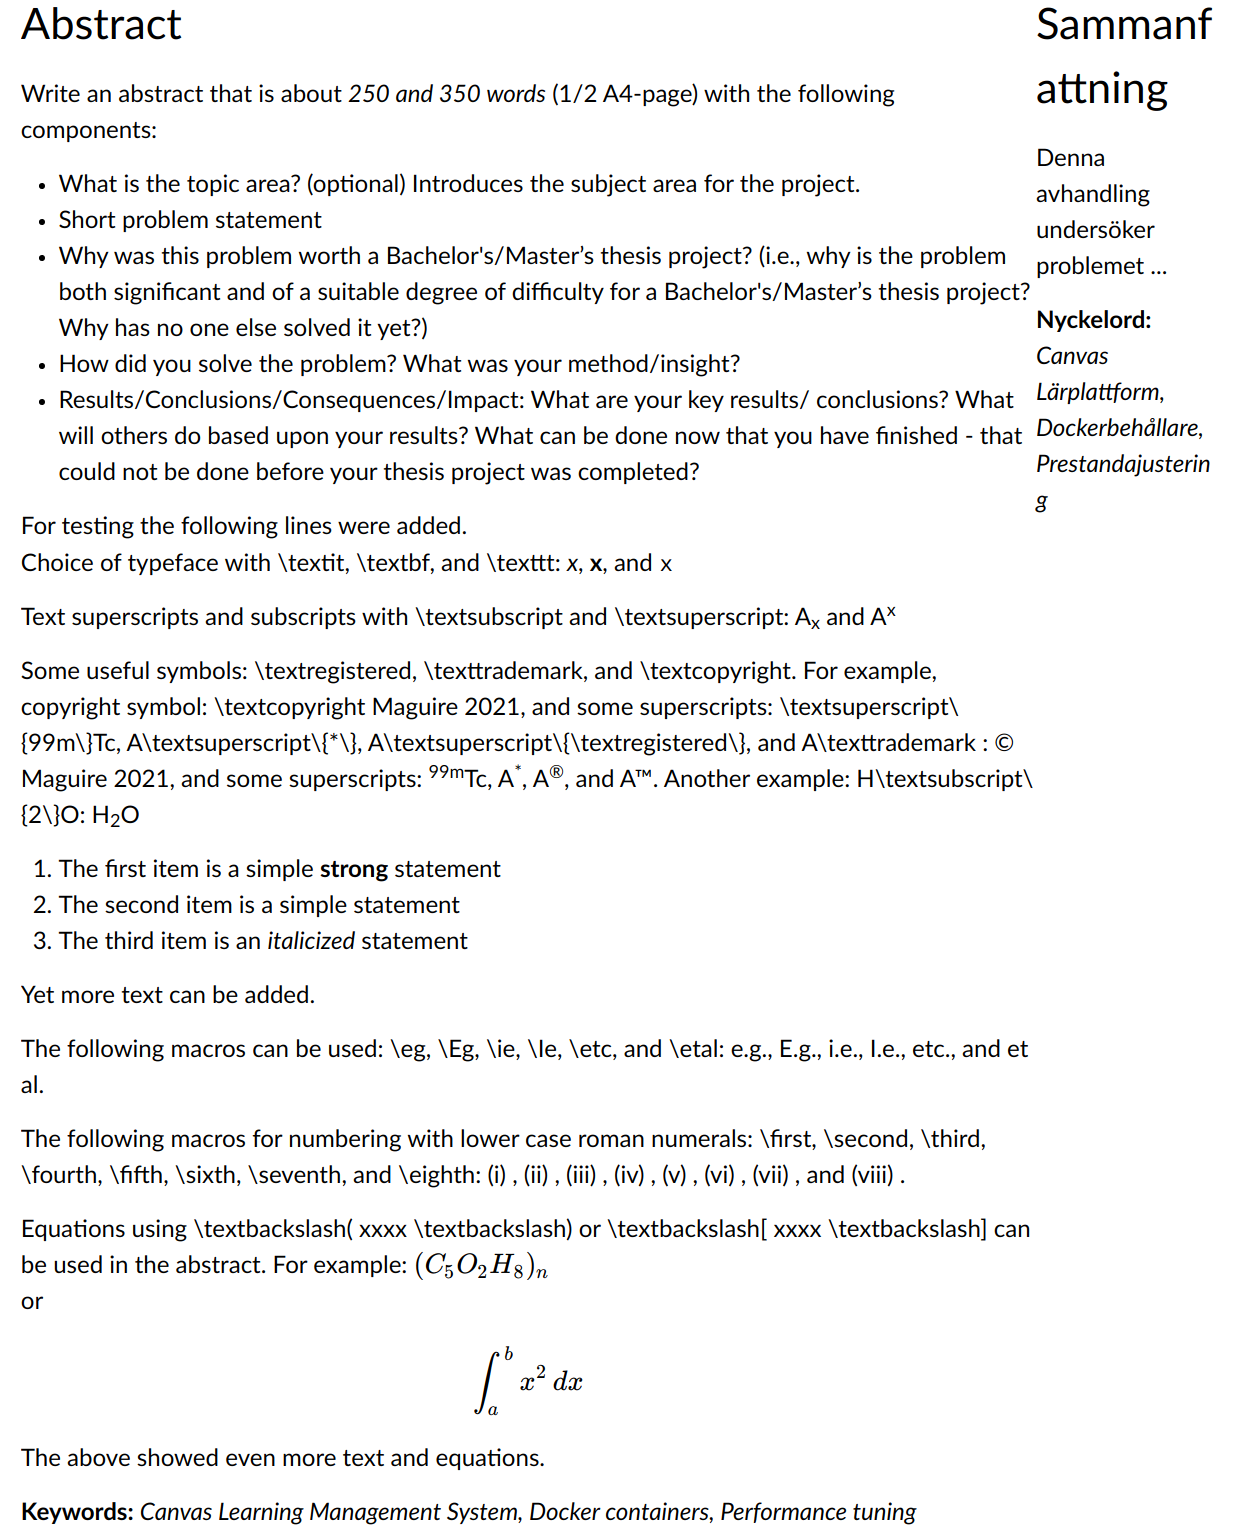
\includegraphics[width=0.5\textwidth]{README_notes/README-examiner-figures/resulting_announcement_109.png}}
  \end{center}
  \caption{Resulting announcement}
  \label{fig:resultingAnnouncementPNG}
\end{figure}
\FloatBarrier


This contrived example shows that a \LaTeX~abstract of the form shown in \Cref{lst:JSONtoLadokK} can be handled. While more testing should be done, this shows that it is possible to directly extract the data that is written to the file as pseudo JSON \LaTeX~\textit{without} having to parse and process the PDF file; however, you still have to compile the \LaTeX~and produce the PDF file in order to produce the \texttt{fordiva.json} file.

\textbf{NB}: that the cleanup\_pseudo\_JSON-from\_LaTeX.py program does simple text substitution and cannot handle nested \LaTeX~commands.

	
\begin{lstlisting}[language={}, caption={Source \LaTeX~(from inside the scontents of the abstract)}, label=lst:JSONtoLadokK]
Write an abstract that is about \textit{250 and 350 words} (1/2 A4-page)  with the following components: % key parts of the abstract
\begin{itemize}
  \item What is the topic area? (optional) Introduces the subject area for the project.
  \item Short problem statement
  \item Why was this problem worth a Bachelor's/Master’s thesis project? (\ie, why is the problem both significant and of a suitable degree of difficulty for a Bachelor's/Master’s thesis project? Why has no one else solved it yet?)
  \item How did you solve the problem? What was your method/insight?
  \item Results/Conclusions/Consequences/Impact: What are your key results/\linebreak[4]conclusions? What will others do based upon your results? What can be done now that you have finished - that could not be done before your thesis project was completed?
\end{itemize}

For testing the following lines were added.
Choice of typeface with \textbackslash textit, \textbackslash textbf, and \textbackslash texttt:  \textit{x}, \textbf{x}, and \texttt{x}

Text superscripts and subscripts with \textbackslash textsubscript and \textbackslash textsuperscript: A\textsubscript{x} and A\textsuperscript{x}

Some useful symbols: \textbackslash textregistered, \textbackslash texttrademark, and \textbackslash textcopyright. For example, copyright symbol: \textbackslash textcopyright Maguire 2021, and some superscripts: \textbackslash textsuperscript\{99m\}Tc, A\textbackslash textsuperscript\{*\}, A\textbackslash textsuperscript\{\textbackslash textregistered\}, and A\textbackslash texttrademark : \textcopyright Maguire 2021, and some superscripts: \textsuperscript{99m}Tc, A\textsuperscript{*}, A\textsuperscript{\textregistered}, and A\texttrademark. Another example: H\textbackslash textsubscript\{2\}O: H\textsubscript{2}O

\begin{enumerate}
  \item The first item is a simple \textbf{strong} statement
  \item The second item is a simple statement
  \item The third item is an \textit{italicized} statement
\end{enumerate}

Yet more text can be added.

The following commands can be used: \textbackslash eg, \textbackslash Eg, \textbackslash ie, \textbackslash Ie, \textbackslash etc, and \textbackslash etal: \eg, \Eg, \ie, \Ie, \etc, and \etal

The following commands for numbering with lower case roman numerals: \textbackslash first, \textbackslash Second, \textbackslash third, \textbackslash fourth, \textbackslash fifth, \textbackslash sixth, \textbackslash seventh, and \textbackslash eighth: \first, \Second, \third, \fourth, \fifth, \sixth, \seventh, and \eighth.

Equations using \textbackslash( xxxx \textbackslash) or \textbackslash[ xxxx \textbackslash] can be used in the abstract. For example: \( (C_5O_2H_8)_n \)
or \[ \int_{a}^{b} x^2 \,dx \]

The above showed even more text and equations.
\end{lstlisting}


The Overleaf project used to workout the string reading and tokenize is at \url{https://www.overleaf.com/read/mqtrxrdcssmg} while the “KTH thesis template for 1\textsuperscript{st} and 2\textsuperscript{nd} cycle degree projects with JSON output” can be found at \url{https://www.overleaf.com/read/gxhwkywbtgsn}.

The reason for adding the reservation “(almost)” in the earlier paragraph was that this file is not directly readable by my programs that could accept the pseudo JSON that I produced with earlier programs. Some of the problems are that the opponents’ name string contains “\&”, \ie it is "A. B. Normal \& A. X. E. Normalè" and this is not acceptable to python’s json.loads{} function; thus, this has to be rewritten. Additionally, the abstracts contain the raw \LaTeX~and thus can include acronyms that need to be spelled out. This means that the same transformations used in \texttt{extract\_pseudo\_JSON-from\_PDF.py} need to be implemented in a new program to clean up the pseudo JSON. This new program is named: \texttt{cleanup\_pseudo\_JSON-from\_LaTeX.py}.

\FloatBarrier

\section{Abstracts in languages that use characters other than those in the main font}
Note that if the user has set the option \texttt{includeExtraAbstracts} and included abstracts that require fonts other than \texttt{TeX Gyre Termes}, the contents of the abstracts in these languages may not appear on the ``For DiVA'' page but will be in the \texttt{fordiva.json} file, unless you add \texttt{\textbackslash newunicodechar} definitions that utilize a font where the characters appearing in the abstract are available.

\begin{listing}[!ht]
\begin{minted}[breaklines, escapeinside=||]{text}
Missing character: There is no 中 (U+4E2D) in font TeX Gyre Cursor/OT:script=latn;language=dflt;-liga;+lnum;+tnum;mapping=tex-text;!
Missing character: There is no 文 (U+6587) in font TeX Gyre Cursor/OT:script=latn;language=dflt;-liga;+lnum;+tnum;mapping=tex-text;!
Missing character: There is no 摘 (U+6458) in font TeX Gyre Cursor/OT:script=latn;language=dflt;-liga;+lnum;+tnum;mapping=tex-text;!
Missing character: There is no 要 (U+8981) in font TeX Gyre Cursor/OT:script=latn;language=dflt;-liga;+lnum;+tnum;mapping=tex-text;!
Missing character: There is no 个 (U+4E2A) in font TeX Gyre Heros/OT:script=latn;language=dflt;mapping=tex-text;!
Missing character: There is no 关 (U+5173) in font TeX Gyre Heros/OT:script=latn;language=dflt;mapping=tex-text;!
Missing character: There is no 键 (U+952E) in font TeX Gyre Heros/OT:script=latn;language=dflt;mapping=tex-text;!
Missing character: There is no 词 (U+8BCD) in font TeX Gyre Heros/OT:script=latn;language=dflt;mapping=tex-text;!
\end{minted}
\caption{Examples of missing characters from the output.log file}
\label{lst:missingCharactersFromLogExample}
\end{listing}

\begin{listing}[!ht]
\begin{minted}[breaklines, escapeinside=||]{text}
\newunicodechar{个}{\iffontchar\font`个 个\else{\cjkfonttt 个}\fi} % U+4E2A - CJK Unified Ideograph-4E2A
\newunicodechar{中}{\iffontchar\font`中 中\else{\cjkfonttt 中}\fi} % U+4E2D - CJK Unified Ideograph-4E2D
\newunicodechar{关}{\iffontchar\font`关 关\else{\cjkfonttt 关}\fi} % U+5173 - CJK Unified Ideograph-5173
\newunicodechar{摘}{\iffontchar\font`摘 摘\else{\cjkfonttt 摘}\fi} % U+6458 - CJK Unified Ideograph-6458
\newunicodechar{文}{\iffontchar\font`文 文\else{\cjkfonttt 文}\fi} % U+6587 - CJK Unified Ideograph-6587
\newunicodechar{要}{\iffontchar\font`要 要\else{\cjkfonttt 要}\fi} % U+8981 - CJK Unified Ideograph-8981
\newunicodechar{词}{\iffontchar\font`词 词\else{\cjkfonttt 词}\fi} % U+8BCD - CJK Unified Ideograph-8BCD
\newunicodechar{键}{\iffontchar\font`键 键\else{\cjkfonttt 键}\fi} % U+952E - CJK Unified Ideograph-952E
\end{minted}
\caption{Examples of new unicode character definitions}
\label{lst:newunicodeForAbstracts}
\end{listing}
\FloatBarrier

%% add more here

\section[Inserting information into LADOK]{Inserting information into LADOK}
\label{sec:JSONtoLADOK}
As part of the effort to be able to minimize the effort of cutting and pasting. I have made a program JSON\_to\_ladok.py that takes the extracted JSON information and uses the information about the author(s) and the title and alternative title to try to insert this information into LADOK for the module (\ie ``moment'' in Swedish) that requires a project title, \ie, 'KravPaProjekttitel' is True. \Cref{lst:usingExtractedJSONtoProduceLADOKentry} shows an example of using this program to try to put the title and alternative title into LADOK. Basically the program logic should work, but I do \textbf{not} have the required permission to make entries of this sort of data for a degree project.

Note that this program uses the \texttt{ladok3} python library but extends it with some features that are not (yet) in the library. It should be regarded as very much a work in progress.
\begin{lstlisting}[language={bash}, caption={Using the extracted JSON to produce a LADOK entry}, label=lst:usingExtractedJSONtoProduceLADOKentry]
./JSON_to_ladok.py -c 11   --json xxx.json   --code DA213X
testing=False
d={'Author1': {'Last name': ‘xxx’, 'First name': 'xxx', 'Local User Id': 'yyyyy', 'E-mail': 'xxx@kth.se', 'organisation': {'L1': 'School of EXXX'}}, 'Degree': {'Educational program': 'Master’s Programme, XXX, 120 credits', 'programcode': 'TXXXX', 'Level': '2', 'Course code': 'XX200X', 'Credits': '30.0', 'Exam': 'Master’s Programme, XXX, 120 credits', 'subjectArea': 'XXX'}, 'Title': {'Main title': 'xxx', 'Subtitle': yyyy', 'Language': 'eng'}, 'Alternative title': {'Main title': 'zzzz', 'Subtitle': wwwww', 'Language': 'swe'}, 'Supervisor1': {'Last name': 'x', 'First name': 'y', 'Local User Id': 'xx', 'E-mail': 'xxxxx@kth.se', 'organisation': {'L1': 'School of XXX', 'L2': 'DepartmentName'}}, 'Supervisor2': {'Last name': 'yyy', 'First name': 'xxx', 'E-mail': 'xxx@zzzz.com', 'Other organisation': ‘zzzz'}, 'Examiner1': {'Last name': 'ExaminersLastname', 'First name': 'ExaminersFirstname', 'Local User Id': 'u1000000', 'E-mail': 'XXX@kth.se', 'organisation': {'L1': 'School of XXX', 'L2': 'DepartmentName'}}, 'Cooperation': {'Partner_name': 'xxx'}, 'National Subject Categories': '10201, 10206', 'Other information': {'Year': '2021', 'Number of pages': 'xix,99'}, 'Opponents': {'Name': 'A. B. Normal & A. X. E. Normalè'}, 'Presentation': {'Date': '2021-03-15 13:00', 'Language': 'eng', 'Room': 'via Zoom', 'Address': 'Isafjordsgatan 22 (Kistagången 16)', 'City': 'Stockholm'}, 'Number of lang instances': '2', 'abstracts': {'eng': xxxx", 'swe': 'yyyy'}, 'keywords': {'eng': 'x, y z', 'swe': x, y, z'}}
course_code=DA231X
author={'Last name': 'xxx', 'First name': 'yyy', 'Local User Id': 'u1xxxx', 'E-mail': 'oxxx@kth.se', 'organisation': {'L1': 'School of XXX'}}
sortable name=X,Y
Canvas user_id=dddd
integration_id=gggggg-gggg-gggg-gggg-ggggggg
ladoK_course_info={'id': 'gggggggg-gggg-gggg-gggg-gggggggggggg', 'round_id': 'gggggggg-gggg-gggg-gggg-gggggggggggg', 'education_id': 'gggggggg-gggg-gggg-gggg-gggggggggggg', 'instance_id': 'gggggggg-gggg-gggg-gggg-gggggggggggg', 'swe_name': 'Examensarbete i XXX, avancerad nivå', 'eng_name': 'Degree Project in XXX, Second Cycle'}
moment code=PRO1, requires title=False
moment code=PRO2, requires title=False
moment code=PRO3, requires title=True
trying to store a passing grade for moment=PRO3
Traceback (most recent call last):
  File "./JSON_to_ladok.py", line 533, in <module>
    sys.exit(main(sys.argv[1:]))
  File "./JSON_to_ ladok.py", line 519, in main
    status=save_result_degree_project3(ladok, integration_id, course_code, mom['Utbildningskod'], '2021-07-14', 'P', "PF", main_title, alternative_main_title)
  File "./JSON_to_ ladok.py", line 374, in save_result_degree_project3
    raise Exception("Couldn't register " + course_moment + "=" + grade_raw + " " + result_date_raw + ": " + r.json()["Meddelande"])
Exception: Couldn't register PRO3=P 2021-07-14: Hinder mot skapa resultat påträffat: Rapporteringsrättighet saknas
\end{lstlisting}


\section{Removing the README\_examiner\_notes}
At some point you will no longer want this README information. You can remove it by removing the line
\textbackslash include\{README\_notes/README\_examiner\_notes\} -- from the \texttt{examplethesis.tex} file. You can then remove the \texttt{README\_notes} directory.

\section[Copyright or Creative Commons License]{Copyright or Creative Commons\\ License}
\label{sec:copyrightOrCClicenseExaminer}
It is possible to have several variants of the bookinfo page:
\begin{enumerate}[labelwidth =\widthof{\textbf{Creative Commons (CC)}}, leftmargin = !]
    \item[copyright] If you want to have a bookinfo page, include the line saying \texttt{\textbackslash bookinfopage}.
    \item[Creative Commons (CC)] If you want to have a bookinfo page but want to have a Creative Commons license, then include \texttt{\textbackslash bookinfopage} and use and configure the \texttt{doclicense} package as shown in Listings \ref{lst:CCBY-NC-ND}, \ref{lst:CCBY-NC-ND-euro}, and \ref{lst:CCzero}.
    \item[none] If you do \textbf{not} want to have a bookinfo page, comment the line saying \texttt{\textbackslash bookinfopage} and add a \texttt{\textbackslash cleardoublepage}.
\end{enumerate}

For background about Creative Commons licenses see:
\url{https://www.kb.se/samverkan-och-utveckling/oppen-tillgang-och-bibsamkonsortiet/open-access-and-bibsam-consortium/open-access/creative-commons-faq-for-researchers.html} and \url{https://kib.ki.se/en/publish-analyse/publish-your-article-open-access/open-licence-your-publication-cc}.

Note that the lowercase version of the license has to be used in the modifier, \ie one of: by, by-nc, by-nd, by-nc-nd, by-sa, by-nc-sa, or zero. For the list of supported licenses see the documentation for the \texttt{doclicense} package.

\begin{lstlisting}[language={[LaTeX]TeX}, caption={Example configuration to have a CC BY-NC-ND license}, label=lst:CCBY-NC-ND]
\usepackage[
    type={CC},
    modifier={by-nc-nd},
    version={4.0},
    hyphenation={RaggedRight},
]{doclicense}
\end{lstlisting}

Note that the option ``hyphenation={RaggedRight}'' can be used with the configuration of the package to set the license information with a ragged right margin rather that as a fill and justified paragraph.

\begin{lstlisting}[language={[LaTeX]TeX}, caption={Example configuration to have a CC BY-NC-ND license with a Euro symbol rather than a Dollar sign}, label=lst:CCBY-NC-ND-euro]
\usepackage[
    type={CC},
    modifier={by-nc-nd},
    version={4.0},
    imagemodifier={-eu-88x31},  % to get Euro symbol rather than Dollar sign
    hyphenation={RaggedRight},
]{doclicense}
\end{lstlisting}

\begin{lstlisting}[language={[LaTeX]TeX}, caption={Example configuration to have a CC0 license}, label=lst:CCzero]
\usepackage[
    type={CC},
    modifier={zero},
    version={1.0},
]{doclicense}
\end{lstlisting}


For someone who is maintaining or modifying the template, it is important to know that the \texttt{\textbackslash bookinfopageCC} command has a case statement in it that uses an internal variable (\texttt{\textbackslash doclicense@modifier}) set by \texttt{doclicense} as shown in~\Cref{lst:bookinfopageCCcaseSTMT}. This case statement will need to be modified if there is a change in the set of Creative Commons licenses. While it might be possible to replace this case statement with \texttt{\textbackslash doclicenseModifier} to directly produce the capitalized version of the license names or perhaps even \texttt{\textbackslash doclicenseName} or \texttt{\textbackslash doclicenseNameRef} to include the capitalized license name as well as the version number (the later also including a URL to the license). However, I think that these alternatives are unnecessary give the \texttt{\textbackslash doclicenseThis} that generates the display of the license with logo(s). More importantly, using these other commands rather than the unprocessed \texttt{\textbackslash doclicense@modifier} lads to problems when writing out the \texttt{fordiva.json} file.

Note that if the \texttt{doclicense} package is used it automatically redefines \texttt{\textbackslash bookinfopage} to be \texttt{\textbackslash bookinfopageCC}.

\begin{lstlisting}[language={[LaTeX]TeX}, caption={Case statement in \textbackslash bookinfopageCC}, label=lst:bookinfopageCCcaseSTMT]
  \IfEqCase{\doclicense@modifier}{%
    {by}{CC BY}%
    {by-nc}{CC BY-NC}%
    {by-nd}{CC BY-ND}%
    {by-nc-nd}{CC BY-NC-ND}%
    {by-sa}{CC BY-SA}%
    {by-nc-sa}{CC BY-NC-SA}%
    {zero}{CC0}%
  }[\typeout{Creative Commons code  \doclicense@modifier not found}\copyright]
\end{lstlisting}

There is a new \texttt{\textbackslash thesiscopyrightleft} command added to the \texttt{\textbackslash bookinfopage} and \texttt{\textbackslash bookinfopageCC} pages to store the value of the copyright or copyleft information that the user chose (if any). This information is later output as information for DiVA in the form shown in \Cref{lst:bookinfoCopyrightselected,lst:bookinfoCopyleftselected,lst:bookinfoNoneselected}
\begin{lstlisting}[language=json, caption={If the user chose to have a copyright on the bookinfo page}, label=lst:bookinfoCopyrightselected]
"Copyrightleft": "copyright"
\end{lstlisting}

\begin{lstlisting}[language=json, caption={If the user chose to have a CC BY-NC license on the bookinfo page}, label=lst:bookinfoCopyleftselected]
"Copyrightleft": "by-nc"
\end{lstlisting}

\begin{lstlisting}[language=json, caption={If the user chose \textbf{not} to have a bookinfo page}, label=lst:bookinfoNoneselected]
"Copyrightleft": "None"
\end{lstlisting}

As a result of adding support for the PDF metadata for the copyright, the template now uses the \texttt{hyperxmp} package. Details of the code to set the value of the pdfcopyright metadata can be seen in \Cref{lst:bookinfopageCopyrightPDFmetadata}.
The use of \texttt{hyperxmp} caused a change in how the author's name is processed - for details about this see \Cref{sec:addingKeywordsAndMetaDataToPDF} starting on page~\pageref{sec:addingKeywordsAndMetaDataToPDF}.

\begin{lstlisting}[language={[LaTeX]TeX}, caption={Processing copyright PDF metadata information in \textbackslash bookinfopageCC}, label=lst:bookinfopageCopyrightPDFmetadata]
% Command to print out the standardized document information page
\newcommand{\bookinfopage}{
\ifgfivepaper
  \newgeometry{top=140mm,bottom=30mm,left=12.25mm,right=35mm}
\else
  \newgeometry{top=250mm,bottom=30mm,left=74pt,right=35mm}
\fi
\thispagestyle{empty}
\begin{flushleft}
  \sffamily
  \copyright\enspace\the\year\quad\@authorsFirstname\space\@authorsLastname 
  \ifx\@secondAuthorsLastname\@empty\relax
  \else
    \ifinswedish
      \enspace och\enspace\@secondAuthorsFirstname\space\@secondAuthorsLastname \\
    \else
      \enspace and\enspace\@secondAuthorsFirstname\space\@secondAuthorsLastname \\
    \fi
  \fi
\end{flushleft}
\thesiscopyrightleft{copyright}
\newcommand{\mycopyright}{%
  {Copyright (c)}\ \the\year\ \@authorsFirstname\ \@authorsLastname %
  \ifx\@secondAuthorsLastname\@empty\relax%
  \else%
    \ifinswedish%
      \  och\ \@secondAuthorsFirstname\ \@secondAuthorsLastname%
    \else%
      \  and\ \@secondAuthorsFirstname\ \@secondAuthorsLastname%
    \fi%
  \fi%
}
\hypersetup{
     pdfcopyright={\mycopyright} 
}
\restoregeometry
\clearpage
}

% bookinfo page with CC license
% CC BY (Attribution)
% CC BY-NC (Attribution + Non-commercial)
% CC BY-ND (Attribution + No derivatives)
% CC BY-NC-ND (Attribution + Non-commercial + No derivatives)
% CC BY-SA (Attribution + ShareAlike)
% CC BY-NC-SA (Attribution + Non-commercial + ShareAlike)
% CC0 (Zero)
\newcommand{\bookinfopageCC}{
\ifgfivepaper
  \newgeometry{top=130mm,bottom=30mm,left=12.25mm,right=35mm}
\else
  \newgeometry{top=220mm,bottom=30mm,left=74pt,right=35mm}
\fi
\thispagestyle{empty}
\begin{flushleft}
  \sffamily
  \IfEqCase{\doclicense@modifier}{%
    {by}{CC BY}%
    {by-nc}{CC BY-NC}%
    {by-nd}{CC BY-ND}%
    {by-nc-nd}{CC BY-NC-ND}%
    {by-sa}{CC BY-SA}%
    {by-nc-sa}{CC BY-NC-SA}%
    {zero}{CC0}%
  }[\typeout{Creative Commons code  \doclicense@modifier not found}\copyright]
  \enspace\the\year\quad\@authorsFirstname\space\@authorsLastname 
  \ifx\@secondAuthorsLastname\@empty\relax
  \else
    \ifinswedish
      \enspace och\enspace\@secondAuthorsFirstname\space\@secondAuthorsLastname \\
    \else
      \enspace and\enspace\@secondAuthorsFirstname\space\@secondAuthorsLastname \\
    \fi
  \fi
  \doclicenseThis
\end{flushleft}
\thesiscopyrightleft{\doclicense@modifier}

\let\@myCC\@empty
\ifdefstring{\doclicense@modifier}{by}{\def\@myCC{CC BY}}
\ifdefstring{\doclicense@modifier}{by-nc}{\def\@myCC{CC BY-NC}}
\ifdefstring{\doclicense@modifier}{by-nd}{\def\@myCC{CC BY-ND}}
\ifdefstring{\doclicense@modifier}{by-nc-nd}{\def\@myCC{CC BY-NC-ND}}
\ifdefstring{\doclicense@modifier}{by-sa}{\def\@myCC{CC BY-SA}}
\ifdefstring{\doclicense@modifier}{by-nc-sa}{\def\@myCC{CC BY-NC-SA}}
\ifdefstring{\doclicense@modifier}{zero}{\def\@myCC{CC0}}

\newcommand{\mycopyright}{%
 \@myCC\ \the\year\ \@authorsFirstname\ \@authorsLastname%
  \ifx\@secondAuthorsLastname\@empty\relax%
  \else%
    \ifinswedish%
      \  och\ \@secondAuthorsFirstname\ \@secondAuthorsLastname%
    \else%
      \ and\ \@secondAuthorsFirstname\ \@secondAuthorsLastname %
    \fi%
  \fi%
}

\hypersetup{
     pdfcopyright={\mycopyright} 
}
\restoregeometry
\clearpage
}

% If the doclicense pacakage is installed, then use the \bookinfoCC when encountering a \bookinfo command
\AtBeginDocument{\@ifpackageloaded{doclicense}
  {%
    \renewcommand{\bookinfopage}{\bookinfopageCC}
  }
  {\relax}
}
\end{lstlisting}

\section[Adding acronyms.tex to For DIVA info]{Adding acronyms.tex to For DIVA info}
\label{sec:acronymsInForDIVAdata}
If the author has used acronyms in the abstract(s), then these acronym definitions need to be available in some way to the person (or program) that makes the MODS file. One solution is to add them at the end of the For DIVA information. This can be done using the code shown in~\Cref{lst:includeAcronymsFile}. This code simply checks for the file and if it is present appends the contents of this file to the text as a listing. An important part to note is the option \texttt{nolol} - this prevents this listing from appearing in the list of listings.

\begin{lstlisting}[language={[LaTeX]TeX}, caption={Code for adding acronyms.tex at the end of the For DIVA data}, label=lst:includeAcronymsFile]
% If there is an acronyms.tex file,
% add it to the end of the For DIVA information
% so that it can be used with the abstracts
% Note that the option "nolol" stops it from being listed in the List of Listings
\IfFileExists{lib/acronyms.tex}{
\section*{acronyms.tex}
\lstinputlisting[language={[LaTeX]TeX}, nolol, basicstyle=\ttfamily\color{black},
commentstyle=\color{black}, backgroundcolor=\color{white}]{lib/acronyms.tex}
}
{}
\end{lstlisting}

\section{Adding additional metadata to the PDF file}
\label{sec:addingMetadataToPDFfile}
It is increasingly the case that metadata is being embedded into digital objects to provide information about the creator (author, photographer, \etc), date of creation, copyright notices, \etc. In a typical PDF file produced by \LaTeX~there is both PDF-specific metadata and additional metadata. This additional metadata is stored using Adobe's Extensible Metadata Platform (XMP). XMP is a means of embedding metadata in XML format into PDF documents so that tools can extract it mechanically.

An early paper about automatically extracting the title, authors(s), and abstract from theses was written by Mao Ni of the University of North Carolina at Chapel Hill, School of Library and Information Science in 2004\,\cite{Mao_Ni_2004}. The idea was to collect the metadata from the thesis using an Adobe Acrobat plugin and then write this data to XMP (which could be embedded into the PDF file). The schema used for the metadata\cite{hickey_pavani_suleman_2010} \footnote{\url{https://ndltd.org/metadata/}} was that of Networked Digital Library of Theses and Dissertations\footnote{\url{https://ndltd.org/}}.

More recently, Elsevier's Digital Commons \footnote{\url{https://www.elsevier.com/solutions/digital-commons}} uses an extension of the Dublin Core\footnote{\url{https://www.dublincore.org/}} shown in \Cref{tab:dublicCoreDigitalCommons} to collect metadata. We will see the Dublin Core elements and others metadata schema used in XMP in the remainder of this section.

Bepress has written about Elsevier's Digital Commons in a webpage ``Digital Commons and OAI-PMH: Outbound Harvesting of Repository Records'' \url{https://bepress.com/reference_guide_dc/digital-commons-oai-harvesting/}. The Open Archives Initiative Protocol for Metadata Harvesting (OAI-PMH) is to foster interoperability between repositories\footnote{\url{https://www.openarchives.org/pmh/}} to enable harvesters to collect metadata from a repository. Over the last 20 years there has been an evolution from simply having metadata in a database that is associated with a publication to an entire ecosystem of metadata and applications - see for example, the twentieth International Conference on Dublin Core and Metadata Applications (DCMI 2022) - \url{https://www.dublincore.org/conferences/2022/programme/}.
\clearpage

\begin{table}[!ht]
    \caption{Dublin Core Elements in Digital Commons\cite{digital_commons_metadata_2016} - items in bold are from the so-called ``simple Dublic Core''}
    \label{tab:dublicCoreDigitalCommons}
    \begin{footnotesize}   
    \begin{tabular}{l | l }
      \textbf{Element} & \textbf{Element} \\
      \hline
\textbf{dc.contributor} & \textbf{dc.rights}\\
dc.contributor.role & dc.rights.accessRights\\
\textbf{dc.coverage} & dc.rights.license\\
dc.coverage.spatial & \textbf{dc.source}\\
dc.coverage.spatial.lat & \textbf{dc.subject}\\
dc.coverage.spatial.long & \textbf{dc.title}\\
dc.coverage.temporal & dc.title.alternative\\
\textbf{dc.creator} & \textbf{dc.type}\\
\textbf{dc.date} & dcam.memberOf\\
dc.date.available & dcterms.accrualMethod\\
dc.date.created & dcterms.accrualPeriodicity\\
dc.date.dateAccepted & dcterms.accrualPolicy\\
dc.date.dateCopyrighted & dcterms.audience\\
dc.date.dateSubmitted & dcterms.audience.educationLevel\\
dc.date.issued & dcterms.audience.mediator\\
dc.date.modified & dcterms.instructionalMethod\\
dc.date.valid & dcterms.provenance\\
\textbf{dc.description} & dcterms.rightsHolder\\
dc.description.abstract & geo.alt\\
dc.description.note & thesis.degree\\
dc.description.release & thesis.degree.discipline\\
dc.description.tableOfContents & thesis.degree.grantor\\
\textbf{dc.format} & thesis.degree.level\\
dc.format.extent & thesis.degree.name\\
dc.format.medium\\
\textbf{dc.identifier}\\
dc.identifier.bibliographicCitation\\
\textbf{dc.language}\\
\textbf{dc.publisher}\\
\textbf{dc.relation}\\
dc.relation.conformsTo\\
dc.relation.hasFormat\\
dc.relation.hasPart\\
dc.relation.hasVersion\\
dc.relation.isFormatOf\\
dc.relation.isPartOf\\
dc.relation.isReferencedBy\\
dc.relation.isReplacedBy\\
dc.relation.isRequiredBy\\
dc.relation.isVersionOf\\
dc.relation.references\\
dc.relation.replaces\\
dc.relation.requires\\
\end{tabular}
\end{footnotesize}
\end{table}
\FloatBarrier
\clearpage

\Cref{fig:fileProperties} shows the properties of a PDF file when using an old version of Adobe Acrobat with the command: File->Properties. This figure shows the Title, Author, Subject, and Keyword fields (among other properties of this PDF file). Because this file was generated in PDF 2.0 format, Acrobat says that you cannot edit the information, and it indicates this by displaying the information in gray.
\begin{figure}[!ht]
  \begin{center}
    \fbox{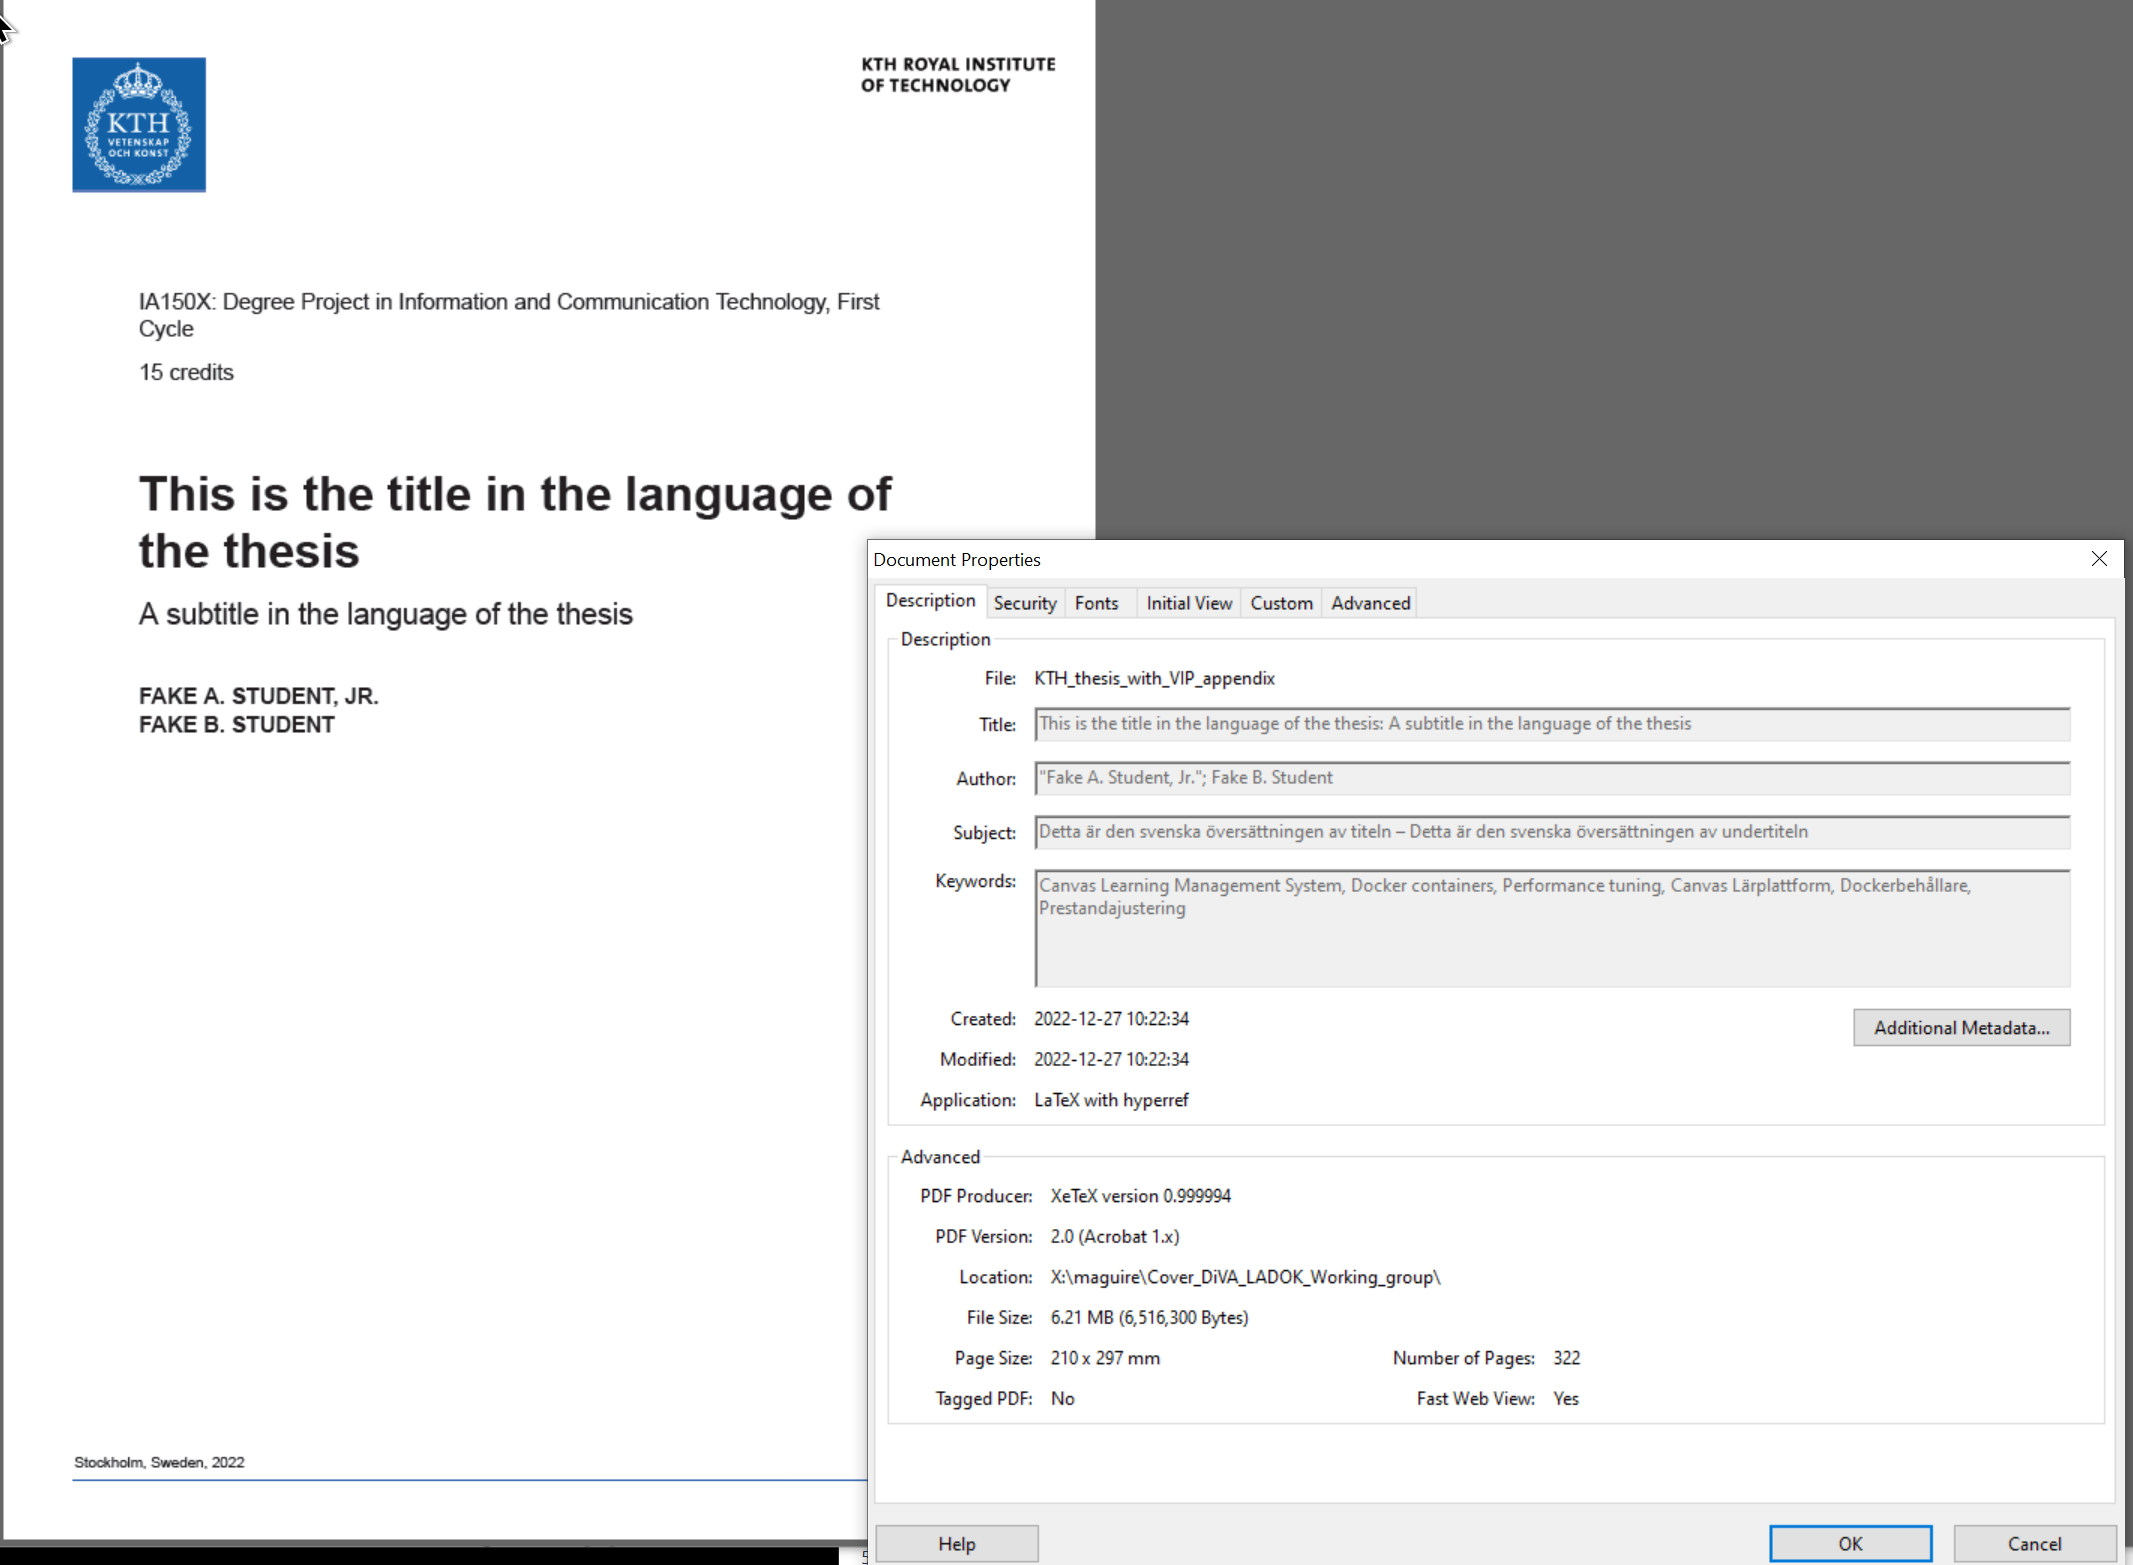
\includegraphics[width=0.9\textwidth]{README_notes/README-examiner-figures/New_thesis_template_document_properties-Screenshot_20221227_115745.png}}
  \end{center}
  \caption{PDF file properties}
  \label{fig:fileProperties}
\end{figure}
\FloatBarrier

\Cref{fig:fileProperties2} shows similar data for another PDF file generated with an earlier PDF version. Because this PDF file uses PDF-1.5, Acrobat displays the information in dark letters, and it is possible to edit the metadata using Acrobat.
\begin{figure}[!ht]
  \begin{center}
    \fbox{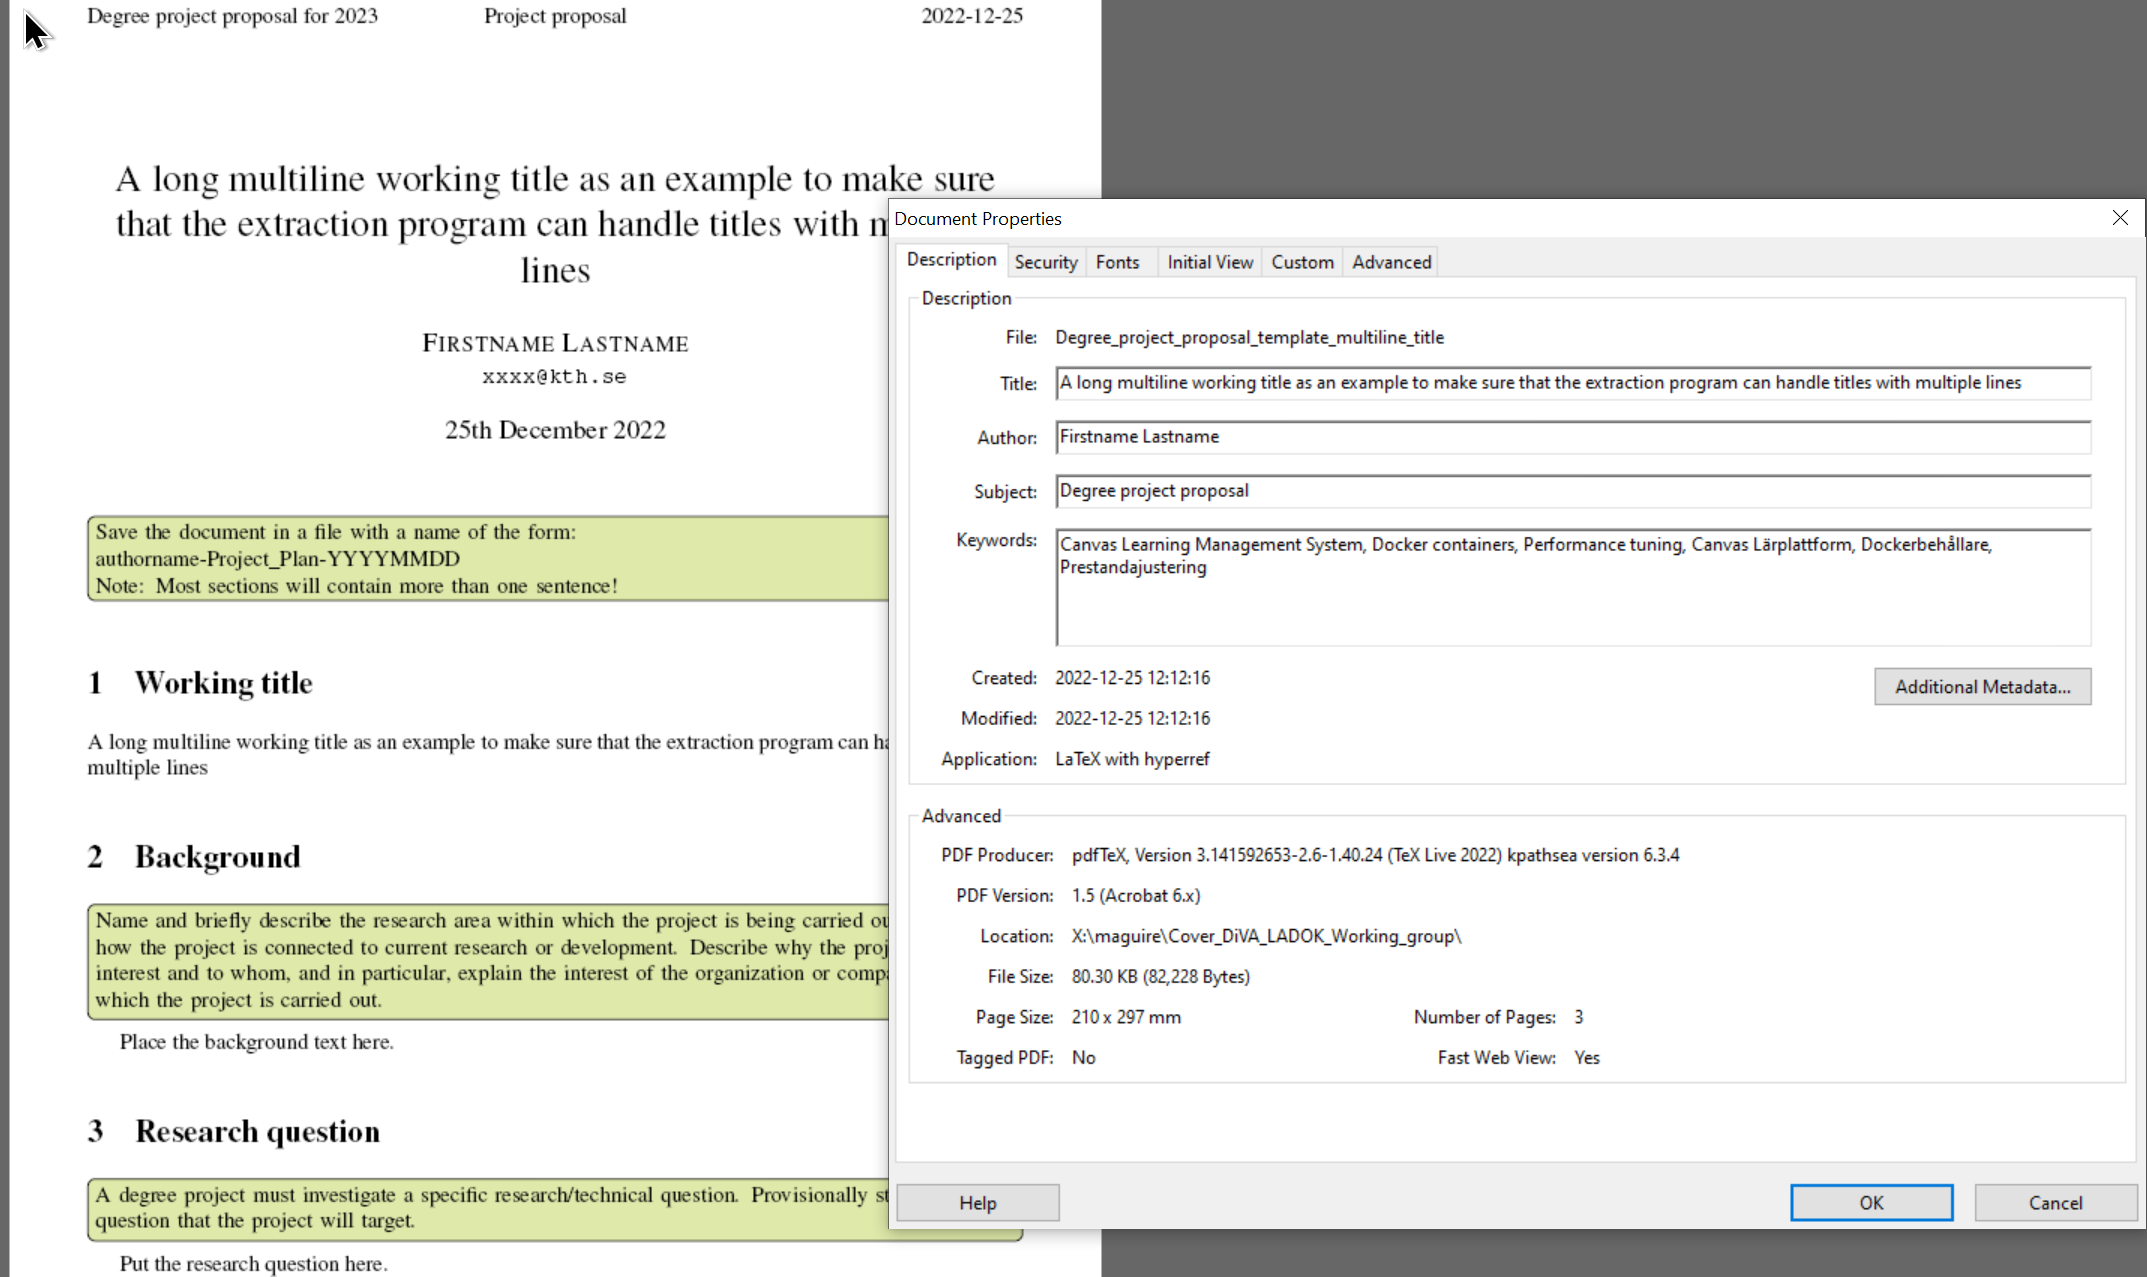
\includegraphics[width=0.9\textwidth]{README_notes/README-examiner-figures/File-properties-Screenshot_20221225_135914.png}}
  \end{center}
  \caption{PDF file properties of another PDF file, in this case, the proposal template}
  \label{fig:fileProperties2}
\end{figure}
\FloatBarrier

The XMP data is in a stream indicated in the PDF as Metadata of the subtype XML, as shown in \Cref{lst:pdfXMPStream}. In the listing, the actual length in bytes has been replaced by dddd.
\begin{lstlisting}[caption={PDF stream where the XMP is found}, label=lst:pdfXMPStream]
<< /Subtype /XML /Type /Metadata /Length dddd >>
stream
\end{lstlisting}

In the PDF file, the XML encoded metadata is between \texttt{<?xpacket begin="yyyy" id="xxxx"?>} and \texttt{<?xpacket end="w"?>} (where xxxx is some unique ID). It is important to note that the value for yyyy in the previous is a so-called byte order marker (BOM) with the value 0xfeff. While this character is a valid \mbox{UTF-8} character, the \texttt{lstlisting} environment cannot handle this value; therefore, it has been replaced by the string ``BOM 0xfeff''. An example of this is shown in \Cref{lst:pdfinfoOutput}.
\clearpage
\begin{lstlisting}[style=myXML,
caption={First part of the XML metadata embedded in a PDF file (some reformatting has been done to fit the text in the boarders)}, label={lst:pdfinfoOutput}]
<?xpacket begin="" id="W5M0MpCehiHzreSzNTczkc9d"?>
<x:xmpmeta xmlns:x="adobe:ns:meta/">
  <rdf:RDF xmlns:rdf="http://www.w3.org/1999/02/22-rdf-syntax-ns#">
    <rdf:Description rdf:about=""
     xmlns:pdf="http://ns.adobe.com/pdf/1.3/"
     xmlns:xmpRights="http://ns.adobe.com/xap/1.0/rights/"
     xmlns:dc="http://purl.org/dc/elements/1.1/"
     xmlns:photoshop="http://ns.adobe.com/photoshop/1.0/"
     xmlns:xmp="http://ns.adobe.com/xap/1.0/"
     xmlns:xmpMM="http://ns.adobe.com/xap/1.0/mm/"
     xmlns:stEvt="http://ns.adobe.com/xap/1.0/sType/ResourceEvent#"
     xmlns:pdfaid="http://www.aiim.org/pdfa/ns/id/"
     xmlns:pdfuaid="http://www.aiim.org/pdfua/ns/id/"
     xmlns:pdfx="http://ns.adobe.com/pdfx/1.3/"
     xmlns:pdfxid="http://www.npes.org/pdfx/ns/id/"
     xmlns:prism="http://prismstandard.org/namespaces/basic/3.0/"
     xmlns:jav="http://www.niso.org/schemas/jav/1.0/"
     xmlns:xmpTPg="http://ns.adobe.com/xap/1.0/t/pg/"
     xmlns:stFnt="http://ns.adobe.com/xap/1.0/sType/Font#"
     xmlns:Iptc4xmpCore="http://iptc.org/std/Iptc4xmpCore/1.0/£\break{\ensuremath{\color{red}\hookrightarrow\space}}£xmlns/"
     xmlns:pdfaExtension="http://www.aiim.org/pdfa/ns/extension/"
     xmlns:pdfaSchema="http://www.aiim.org/pdfa/ns/schema#"
     xmlns:pdfaProperty="http://www.aiim.org/pdfa/ns/property#"
     xmlns:pdfaType="http://www.aiim.org/pdfa/ns/type#"
     xmlns:pdfaField="http://www.aiim.org/pdfa/ns/field#">
\end{lstlisting}

Some of these XML elements include "rdf" elements referring to the Resource Description Framework (RDF)\footnote{\url{https://www.w3.org/RDF/}}.

The XMP data utilizes a number of different schema and namespaces. These namespaces are shown as ``xmlns:xxxx''  in \Cref{lst:pdfinfoOutput}. One namespace is \texttt{xmlns:dc} and this refers to the scheme is `Dublin Core'' \footnote{see Dublin Core Metadata Initiative \url{https://www.dublincore.org/}}. The information about this namespace can be found at \url{http://purl.org/dc/elements/1.1/}. Each of the schema and namespace are described in the next part of the XML, see \Cref{lst:pdfinfoOutputPart2}.

\begin{lstlisting}[style=myXML,
caption={Second part of the XML metadata embedded in a PDF file (some reformatting has been done to fit the text in the boarders)}, label={lst:pdfinfoOutputPart2}]
£$\ldots$ {\color{red} continuation of the above listing}£ 
      <pdfaExtension:schemas>
        <rdf:Bag>
          <rdf:li rdf:parseType="Resource">
            <pdfaSchema:schema>Adobe PDF Schema</pdfaSchema:schema>
            <pdfaSchema:prefix>pdf</pdfaSchema:prefix>
            <pdfaSchema:namespaceURI>http://ns.adobe.com/pdf/1.3/£\break{\ensuremath{\color{red}\hookrightarrow\space}}£</pdfaSchema:namespaceURI>
            <pdfaSchema:property>
              <rdf:Seq>
                <rdf:li rdf:parseType="Resource">
                  <pdfaProperty:name>Trapped</pdfaProperty:name>
                  <pdfaProperty:valueType>Text</pdfaProperty:valueType>
                  <pdfaProperty:category>internal</pdfaProperty:category>
                  <pdfaProperty:description>Indication if the document has been modified to include trapping information</pdfaProperty:description>
                </rdf:li>
              </rdf:Seq>
            </pdfaSchema:property>
          </rdf:li>
          <rdf:li rdf:parseType="Resource">
            <pdfaSchema:schema>XMP Media Management Schema</pdfaSchema:schema>
            <pdfaSchema:prefix>xmpMM</pdfaSchema:prefix>
            <pdfaSchema:namespaceURI>http://ns.adobe.com/xap/1.0/mm/£\break{\ensuremath{\color{red}\hookrightarrow\space}}£</pdfaSchema:namespaceURI>
            <pdfaSchema:property>
              <rdf:Seq>
                <rdf:li rdf:parseType="Resource">
                  <pdfaProperty:name>DocumentID</pdfaProperty:name>
                  <pdfaProperty:valueType>URI</pdfaProperty:valueType>
                  <pdfaProperty:category>internal</pdfaProperty:category>
                  <pdfaProperty:description>UUID based identifier for all versions and renditions of a document</pdfaProperty:description>
                </rdf:li>
                <rdf:li rdf:parseType="Resource">
                  <pdfaProperty:name>InstanceID</pdfaProperty:name>
                  <pdfaProperty:valueType>URI</pdfaProperty:valueType>
                  <pdfaProperty:category>internal</pdfaProperty:category>
                  <pdfaProperty:description>UUID based identifier for specific incarnation of a document</pdfaProperty:description>
                </rdf:li>
                <rdf:li rdf:parseType="Resource">
                  <pdfaProperty:name>VersionID</pdfaProperty:name>
                  <pdfaProperty:valueType>Text</pdfaProperty:valueType>
                  <pdfaProperty:category>internal</pdfaProperty:category>
                  <pdfaProperty:description>Document version identifier</pdfaProperty:description>
                </rdf:li>
                <rdf:li rdf:parseType="Resource">
                  <pdfaProperty:name>RenditionClass</pdfaProperty:name>
                  <pdfaProperty:valueType>RenditionClass</pdfaProperty:valueType>
                  <pdfaProperty:category>internal</pdfaProperty:category>
                  <pdfaProperty:description>The manner in which a document is rendered</pdfaProperty:description>
                </rdf:li>
              </rdf:Seq>
            </pdfaSchema:property>
          </rdf:li>
          <rdf:li rdf:parseType="Resource">
            <pdfaSchema:schema>IPTC Core Schema</pdfaSchema:schema>
            <pdfaSchema:prefix>Iptc4xmpCore</pdfaSchema:prefix>
            <pdfaSchema:namespaceURI>http://iptc.org/std/Iptc4xmpCore/1.0/xmlns/£\break{\ensuremath{\color{red}\hookrightarrow\space}}£</pdfaSchema:namespaceURI>
            <pdfaSchema:property>
              <rdf:Seq>
                <rdf:li rdf:parseType="Resource">
                  <pdfaProperty:name>CreatorContactInfo</pdfaProperty:name>
                  <pdfaProperty:valueType>ContactInfo</pdfaProperty:valueType>
                  <pdfaProperty:category>external</pdfaProperty:category>
                  <pdfaProperty:description>Document creator's contact information</pdfaProperty:description>
                </rdf:li>
              </rdf:Seq>
            </pdfaSchema:property>
            <pdfaSchema:valueType>
              <rdf:Seq>
                <rdf:li rdf:parseType="Resource">
                  <pdfaType:type>ContactInfo</pdfaType:type>
                  <pdfaType:namespaceURI>http://iptc.org/std/Iptc4xmpCore/1.0/xmlns/£\break{\ensuremath{\color{red}\hookrightarrow\space}}£</pdfaType:namespaceURI>
                  <pdfaType:prefix>Iptc4xmpCore</pdfaType:prefix>
                  <pdfaType:description>Basic set of information to get in contact with a person</pdfaType:description>
                  <pdfaType:field>
                    <rdf:Seq>
                      <rdf:li rdf:parseType="Resource">
                        <pdfaField:name>CiAdrCity</pdfaField:name>
                        <pdfaField:valueType>Text</pdfaField:valueType>
                        <pdfaField:description>Contact information city</pdfaField:description>
                      </rdf:li>
                      <rdf:li rdf:parseType="Resource">
                        <pdfaField:name>CiAdrCtry</pdfaField:name>
                        <pdfaField:valueType>Text</pdfaField:valueType>
                        <pdfaField:description>Contact information country</pdfaField:description>
                      </rdf:li>
                      <rdf:li rdf:parseType="Resource">
                        <pdfaField:name>CiAdrExtadr</pdfaField:name>
                        <pdfaField:valueType>Text</pdfaField:valueType>
                        <pdfaField:description>Contact information address</pdfaField:description>
                      </rdf:li>
                      <rdf:li rdf:parseType="Resource">
                        <pdfaField:name>CiAdrPcode</pdfaField:name>
                        <pdfaField:valueType>Text</pdfaField:valueType>
                        <pdfaField:description>Contact information local postal code</pdfaField:description>
                      </rdf:li>
                      <rdf:li rdf:parseType="Resource">
                        <pdfaField:name>CiAdrRegion</pdfaField:name>
                        <pdfaField:valueType>Text</pdfaField:valueType>
                        <pdfaField:description>Contact information regional information such as state or province</pdfaField:description>
                      </rdf:li>
                      <rdf:li rdf:parseType="Resource">
                        <pdfaField:name>CiEmailWork</pdfaField:name>
                        <pdfaField:valueType>Text</pdfaField:valueType>
                        <pdfaField:description>Contact information email address(es)</pdfaField:description>
                      </rdf:li>
                      <rdf:li rdf:parseType="Resource">
                        <pdfaField:name>CiTelWork</pdfaField:name>
                        <pdfaField:valueType>Text</pdfaField:valueType>
                        <pdfaField:description>Contact information telephone number(s)</pdfaField:description>
                      </rdf:li>
                      <rdf:li rdf:parseType="Resource">
                        <pdfaField:name>CiUrlWork</pdfaField:name>
                        <pdfaField:valueType>Text</pdfaField:valueType>
                        <pdfaField:description>Contact information Web URL(s)</pdfaField:description>
                      </rdf:li>
                    </rdf:Seq>
                  </pdfaType:field>
                </rdf:li>
              </rdf:Seq>
            </pdfaSchema:valueType>
          </rdf:li>
          <rdf:li rdf:parseType="Resource">
            <pdfaSchema:schema>PRISM Basic Metadata</pdfaSchema:schema>
            <pdfaSchema:prefix>prism</pdfaSchema:prefix>
            <pdfaSchema:namespaceURI>http://prismstandard.org/namespaces/basic/3.0/£\break{\ensuremath{\color{red}\hookrightarrow\space}}£</pdfaSchema:namespaceURI>
            <pdfaSchema:property>
              <rdf:Seq>
                <rdf:li rdf:parseType="Resource">
                  <pdfaProperty:name>complianceProfile</pdfaProperty:name>
                  <pdfaProperty:valueType>Text</pdfaProperty:valueType>
                  <pdfaProperty:category>internal</pdfaProperty:category>
                  <pdfaProperty:description>PRISM specification compliance profile to which this document adheres</pdfaProperty:description>
                </rdf:li>
                <rdf:li rdf:parseType="Resource">
                  <pdfaProperty:name>publicationName</pdfaProperty:name>
                  <pdfaProperty:valueType>Text</pdfaProperty:valueType>
                  <pdfaProperty:category>external</pdfaProperty:category>
                  <pdfaProperty:description>Publication name</pdfaProperty:description>
                </rdf:li>
                <rdf:li rdf:parseType="Resource">
                  <pdfaProperty:name>aggregationType</pdfaProperty:name>
                  <pdfaProperty:valueType>Text</pdfaProperty:valueType>
                  <pdfaProperty:category>external</pdfaProperty:category>
                  <pdfaProperty:description>Publication type</pdfaProperty:description>
                </rdf:li>
                <rdf:li rdf:parseType="Resource">
                  <pdfaProperty:name>bookEdition</pdfaProperty:name>
                  <pdfaProperty:valueType>Text</pdfaProperty:valueType>
                  <pdfaProperty:category>external</pdfaProperty:category>
                  <pdfaProperty:description>Edition of the book in which the document was published</pdfaProperty:description>
                </rdf:li>
                <rdf:li rdf:parseType="Resource">
                  <pdfaProperty:name>volume</pdfaProperty:name>
                  <pdfaProperty:valueType>Text</pdfaProperty:valueType>
                  <pdfaProperty:category>external</pdfaProperty:category>
                  <pdfaProperty:description>Publication volume number</pdfaProperty:description>
                </rdf:li>
                <rdf:li rdf:parseType="Resource">
                  <pdfaProperty:name>number</pdfaProperty:name>
                  <pdfaProperty:valueType>Text</pdfaProperty:valueType>
                  <pdfaProperty:category>external</pdfaProperty:category>
                  <pdfaProperty:description>Publication issue number within a volume</pdfaProperty:description>
                </rdf:li>
                <rdf:li rdf:parseType="Resource">
                  <pdfaProperty:name>pageRange</pdfaProperty:name>
                  <pdfaProperty:valueType>Text</pdfaProperty:valueType>
                  <pdfaProperty:category>external</pdfaProperty:category>
                  <pdfaProperty:description>Page range for the document within the print version of its publication</pdfaProperty:description>
                </rdf:li>
                <rdf:li rdf:parseType="Resource">
                  <pdfaProperty:name>issn</pdfaProperty:name>
                  <pdfaProperty:valueType>Text</pdfaProperty:valueType>
                  <pdfaProperty:category>external</pdfaProperty:category>
                  <pdfaProperty:description>ISSN for the printed publication in which the document was published</pdfaProperty:description>
                </rdf:li>
                <rdf:li rdf:parseType="Resource">
                  <pdfaProperty:name>eIssn</pdfaProperty:name>
                  <pdfaProperty:valueType>Text</pdfaProperty:valueType>
                  <pdfaProperty:category>external</pdfaProperty:category>
                  <pdfaProperty:description>ISSN for the electronic publication in which the document was published</pdfaProperty:description>
                </rdf:li>
                <rdf:li rdf:parseType="Resource">
                  <pdfaProperty:name>isbn</pdfaProperty:name>
                  <pdfaProperty:valueType>Text</pdfaProperty:valueType>
                  <pdfaProperty:category>external</pdfaProperty:category>
                  <pdfaProperty:description>ISBN for the publication in which the document was published</pdfaProperty:description>
                </rdf:li>
                <rdf:li rdf:parseType="Resource">
                  <pdfaProperty:name>doi</pdfaProperty:name>
                  <pdfaProperty:valueType>Text</pdfaProperty:valueType>
                  <pdfaProperty:category>external</pdfaProperty:category>
                  <pdfaProperty:description>Digital Object Identifier for the document</pdfaProperty:description>
                </rdf:li>
                <rdf:li rdf:parseType="Resource">
                  <pdfaProperty:name>url</pdfaProperty:name>
                  <pdfaProperty:valueType>URL</pdfaProperty:valueType>
                  <pdfaProperty:category>external</pdfaProperty:category>
                  <pdfaProperty:description>URL at which the document can be found</pdfaProperty:description>
                </rdf:li>
                <rdf:li rdf:parseType="Resource">
                  <pdfaProperty:name>byteCount</pdfaProperty:name>
                  <pdfaProperty:valueType>Integer</pdfaProperty:valueType>
                  <pdfaProperty:category>internal</pdfaProperty:category>
                  <pdfaProperty:description>Approximate file size in octets</pdfaProperty:description>
                </rdf:li>
                <rdf:li rdf:parseType="Resource">
                  <pdfaProperty:name>pageCount</pdfaProperty:name>
                  <pdfaProperty:valueType>Integer</pdfaProperty:valueType>
                  <pdfaProperty:category>internal</pdfaProperty:category>
                  <pdfaProperty:description>Number of pages in the print version of the document</pdfaProperty:description>
                </rdf:li>
                <rdf:li rdf:parseType="Resource">
                  <pdfaProperty:name>subtitle</pdfaProperty:name>
                  <pdfaProperty:valueType>Text</pdfaProperty:valueType>
                  <pdfaProperty:category>external</pdfaProperty:category>
                  <pdfaProperty:description>Document's subtitle</pdfaProperty:description>
                </rdf:li>
              </rdf:Seq>
            </pdfaSchema:property>
          </rdf:li>
        </rdf:Bag>
      </pdfaExtension:schemas>
\end{lstlisting}

\Cref{lst:pdfinfoOutputPart3} shows the third part of the XMP data. In this part we can see information in the \texttt{pdf} namespace. Information about this namespace should be found at \url{http://ns.adobe.com/pdf/1.3/}; however, this URL is no longer valid - but one can find the data at \url{https://developer.adobe.com/xmp/docs/XMPNamespaces/pdf/}. The Adobe PDF namespace has defined four names: pdf:Keywords, pdf:PDFVersion, pdf:Producer, and pdf:Trapped. In this listing we can see two of these: pdf:Producer and pdf:Keywords. The latter of these is a comma separated list of keywords.
\begin{lstlisting}[style=myXML,
caption={The \texttt{pdf}-prefix metadata embedded in a PDF file (some reformatting has been done to fit the text in the boarders)}, label={lst:pdfinfoOutputPart3}]
£$\ldots$ {\color{red} continuation of the above listing}£ 
      <pdf:Producer>XeTeX version 0.999994</pdf:Producer>
      <pdf:Keywords>Canvas Learning Management System, Docker containers, Performance tuning, Canvas Lärplattform, Dockerbehållare, Prestandajustering</pdf:Keywords>
\end{lstlisting}

\Cref{lst:pdfinfoOutputPart4} shows the next part of the XMP data. In this case we see a new name prefix \texttt{xmpRights}, specifically the name \texttt{xmpRights:Marked}. This namespace should be described at \url{http://ns.adobe.com/xap/1.0/rights/}; however, this URL is no longer valid - but one can find the information at \url{https://developer.adobe.com/xmp/docs/XMPNamespaces/xmpRights/}. This namespace defines the following names: xmpRights:Certificate, xmpRights:Marked, xmpRights:Owner, xmpRights:UsageTerms, and xmpRights:WebStatement. In this case xmpRights:Marked is marked as ``True'' which ``indicates that this is a rights-managed resource. When false, indicates that this is a public-domain resource. Omit if the state is unknown.''. So in this case it is a right-managed resource.
\begin{lstlisting}[style=myXML,
caption={The \texttt{xmpRights:Marked} metadata embedded in a PDF file}, label={lst:pdfinfoOutputPart4}]
£$\ldots$ {\color{red} continuation of the above listing}£ 
      <xmpRights:Marked>True</xmpRights:Marked>
\end{lstlisting}

\Cref{lst:pdfinfoOutputPart5} shows the next part of the XMP data. In this case we can see an element from the \texttt{dc} namespace. The name \texttt{dc:format} indicates the format of the document. As per \url{https://www.dublincore.org/specifications/dublin-core/format-element/} in the case of an electronic document the format is described using the Internet Media Types (\ie MIME values).
\begin{lstlisting}[style=myXML,
caption={The \texttt{dc:format} metadata embedded in a PDF file}, label={lst:pdfinfoOutputPart5}]
£$\ldots$ {\color{red} continuation of the above listing}£ 
      <dc:format>application/pdf</dc:format>
\end{lstlisting}

\Cref{lst:pdfinfoOutputPart6} shows the next part of the XMP data. In this case, we can see another element from the \texttt{dc} namespace. More specifically the element named \texttt{dc:title} and this contains the title of the document. This also illustrates another feature of the XML -- it is possible to have the title in several different languages. The RDF tag \texttt{rdf:Alt} indicates that there are a list of alternatives. In this case the items in the list are tagged with a language tag. The language tag \texttt{xml:lang="x-default"} is the default language of the document. This is followed by items what contain the English (tagged ``en'') and Swedish (tagged ``sv''). The language tags are an ISO 639-1 two-letter language code with an
optional ISO 3166-1 two-letter region code.
\begin{lstlisting}[style=myXML,
caption={The \texttt{dc:title>} metadata embedded in a PDF file (some reformatting has been done to fit the text in the boarders)}, label={lst:pdfinfoOutputPart6}]
£$\ldots$ {\color{red} continuation of the above listing}£ 
      <dc:title>
        <rdf:Alt>
          <rdf:li xml:lang="x-default">This is the title in the language of the thesis: A subtitle in the language of the thesis</rdf:li>
          <rdf:li xml:lang="en">This is the title in the language of the thesis: A subtitle in the language of the thesis</rdf:li>
          <rdf:li xml:lang="sv">Detta är den svenska översättningen av titeln – Detta är den svenska översättningen av undertiteln</rdf:li>
        </rdf:Alt>
      </dc:title>
\end{lstlisting}

\Cref{lst:pdfinfoOutputPart7} shows the \texttt{dc:description} metadata. These contain the abstracts in each of the languages used in the thesis. This is done using the same mechanism as described above for the titles. Note that is possible to use \LaTeX~macros in the abstracts, but the set of things that are supported by subsequent post-processing is limited. The \LaTeX~macros are hidden from expansion by replacing all instances of '\textbackslash' with '\textcent' (the cent symbol) using a new macro: \textbackslash replaceBS defined in \texttt{kththesis.cls}.
\begin{lstlisting}[style=myXML,
caption={The \texttt{dc:description} metadata embedded in a PDF file (some reformatting has been done to fit the text in the boarders)}, label={lst:pdfinfoOutputPart7}]
£$\ldots$ {\color{red} continuation of the above listing}£ 
      <dc:description>
        <rdf:Alt>
          <rdf:li xml:lang="x-default">Detta är den svenska översättningen av titeln – Detta är den svenska översättningen av undertiteln</rdf:li>
          <rdf:li xml:lang="en">Detta är den svenska översättningen av titeln – Detta är den svenska översättningen av undertiteln</rdf:li>
          <rdf:li xml:lang="sv">Detta är den svenska översättningen av titeln – Detta är den svenska översättningen av undertiteln</rdf:li>
          <rdf:li xml:lang="en-US">abstract: "¢generalExpl{Enter your abstract here!}
Write an abstract that is about 250 and 350 words (1/2 A4-page)  with the following components:
% key parts of the abstract
¢begin{itemize}
  ¢item What is the topic area? (optional) Introduces the subject area for the project.
  ¢item Short problem statement
  ¢item Why was this problem worth a Bachelor's/Master’s thesis project? (¢ie, why is the problem both significant and of a suitable degree of difficulty for a Bachelor's/Master’s thesis project? Why has no one else solved it yet?)
  ¢item How did you solve the problem? What was your method/insight?
  ¢item Results/Conclusions/Consequences/Impact: What are your key results/¢linebreak[4]conclusions? What will others do based upon your results? What can be done now that you have finished - that could not be done before your thesis project was completed?
¢end{itemize}
"</rdf:li>
          <rdf:li xml:lang="sv">abstract: "¢generalExpl{Enter your Swedish abstract or summary here!}
¢sweExpl{Alla avhandlingar vid KTH ¢textbf{måste ha} ett abstrakt på både ¢textit{engelska} och ¢textit{svenska}.¢¢
Om du skriver din avhandling på svenska ska detta göras först (och placera det som det första abstraktet) - och du bör revidera det vid behov.}

¢engExpl{If you are writing your thesis in English, you can leave this until the draft version that goes to your opponent for the written opposition. In this way you can provide the English and Swedish abstract/summary information that can be used in the announcement for your oral presentation.¢¢If you are writing your thesis in English, then this section can be a summary targeted at a more general reader. However, if you are writing your thesis in Swedish, then the reverse is true – your abstract should be for your target audience, while an English summary can be written targeted at a more general audience.¢¢This means that the English abstract and Swedish sammnfattning
or Swedish abstract and English summary need not be literal translations of each other.}

¢warningExpl{Do not use the ¢textbackslash glspl¢{¢} command in an abstract that is not in English, as my programs do not know how to generate plurals in other languages. Instead you will need to spell these terms out or give the proper plural form. In fact, it is a good idea not to use the glossary commands at all in an abstract/summary in a language other than the language used in the ¢texttt{acronyms.tex file} - since the glossary package does ¢textbf{not} support use of more than one language.}

¢engExpl{The abstract in the language used for the thesis should be the first abstract, while the Summary/Sammanfattning in the other language can follow}"</rdf:li>
          <rdf:li xml:lang="fr-FR">abstract: "Résumé en français."</rdf:li>
          <rdf:li xml:lang="es-ES">abstract: "Résumé en espagnol."</rdf:li>
          <rdf:li xml:lang="it">abstract: "Sommario in italiano."</rdf:li>
          <rdf:li xml:lang="nb">abstract: "Sammendrag på norsk."</rdf:li>
          <rdf:li xml:lang="de-DE">abstract: "Zusammenfassung in Deutsch."</rdf:li>
          <rdf:li xml:lang="da">abstract: "Abstrakt på dansk."</rdf:li>
          <rdf:li xml:lang="nl">abstract: "Samenvatting in het Nederlands."</rdf:li>
          <rdf:li xml:lang="et">abstract: "Eesti keeles kokkuvõte."</rdf:li>
        </rdf:Alt>
      </dc:description>
\end{lstlisting}

\Cref{lst:pdfinfoOutputPart8} shows the \texttt{dc:rights}, \texttt{dc:publisher}, \texttt{dc:date}, and \texttt{dc:type} elements. The \textbackslash bookinfomacro was extended to put the copyright information into the metadata. This metadata and the \texttt{xmpRights:Marked} value being \textbf{True} enables the display of the copyright data as shown in \Cref{fig:exampleCopyrightXMPdisplayed}.

\begin{lstlisting}[style=myXML,
caption={The \texttt{dc:rights}, \texttt{dc:publisher}, \texttt{dc:date}, and \texttt{dc:type} metadata embedded in a PDF file (some reformatting has been done to fit the text in the boarders)}, label={lst:pdfinfoOutputPart8}]
£$\ldots$ {\color{red} continuation of the above listing}£ 
      <dc:rights>
        <rdf:Alt>
          <rdf:li xml:lang="en">Copyright (c) 2022 Fake A. Student, Jr. and Fake B. Student</rdf:li>
        </rdf:Alt>
      </dc:rights>
      <dc:publisher>
        <rdf:Bag>
          <rdf:li>KTH Royal Institute of Technology</rdf:li>
        </rdf:Bag>
      </dc:publisher>
      <dc:date>
        <rdf:Seq>
          <rdf:li>2022-12-27T10:22:34Z</rdf:li>
        </rdf:Seq>
      </dc:date>
      <dc:type>
        <rdf:Bag>
          <rdf:li>Text</rdf:li>
        </rdf:Bag>
      </dc:type>
\end{lstlisting}

 	
\begin{figure}[!ht]
  \begin{center}
    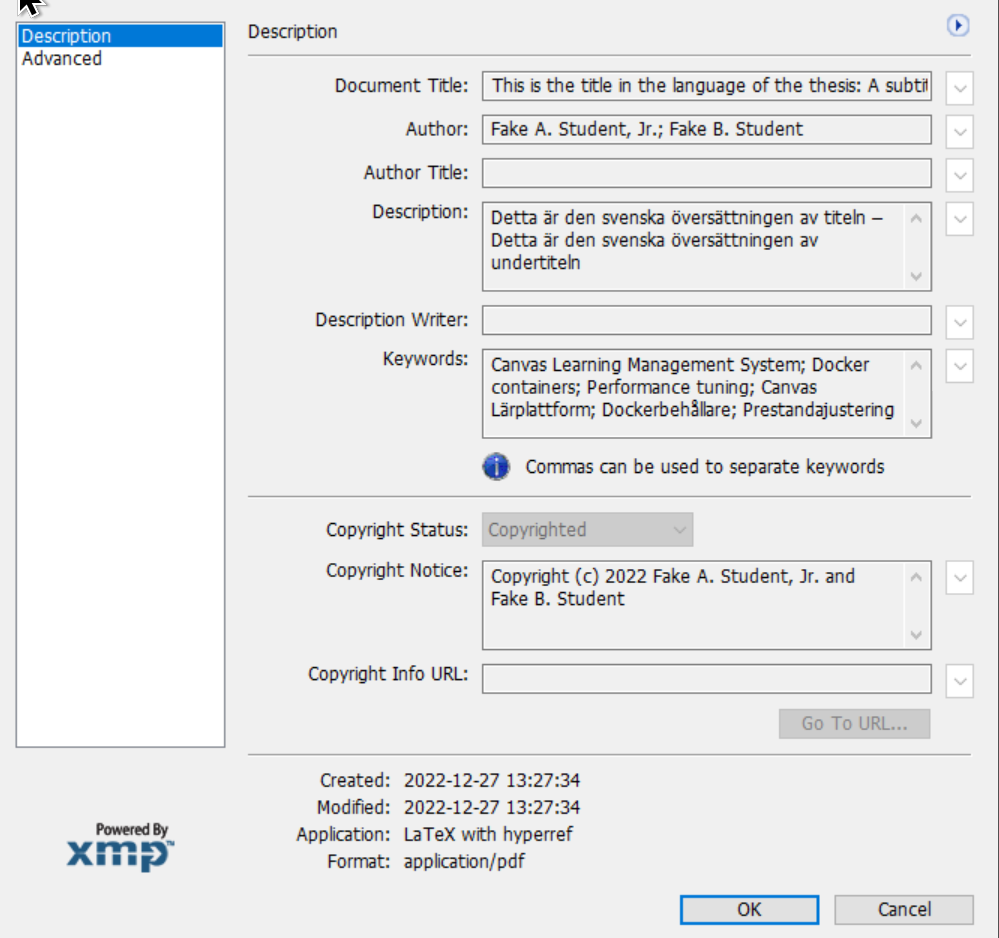
\includegraphics[width=0.99\textwidth]{README_notes/README-examiner-figures/Example-of-copyright-data-Screenshot_20221227_143035.png}
  \end{center}
  \caption{Example of the copyright information being displayed}
  \label{fig:exampleCopyrightXMPdisplayed}
\end{figure}

\Cref{lst:pdfinfoOutputPart9} shows the \texttt{dc:creator} metadata. In this case the comma separated list of authors has been rendered as an \texttt{rdf:Seq} which is an \textbf{ordered} list of items.
\begin{lstlisting}[style=myXML,
caption={The \texttt{dc:creator} metadata embedded in a PDF file}, label={lst:pdfinfoOutputPart9}]
£$\ldots$ {\color{red} continuation of the above listing}£ 
      <dc:creator>
        <rdf:Seq>
          <rdf:li>Fake A. Student, Jr.</rdf:li>
          <rdf:li>Fake B. Student</rdf:li>
        </rdf:Seq>
      </dc:creator>
\end{lstlisting}
\clearpage

\Cref{lst:pdfinfoOutputPart10} shows the \texttt{dc:subject} metadata. In this case the comma separated list of keywords has been rendered as an \texttt{rdf:Bag} which is an \textbf{unordered} list of items.
\begin{lstlisting}[style=myXML,
caption={The \texttt{dc:subject} metadata embedded in a PDF file}, label={lst:pdfinfoOutputPart10}]
£$\ldots$ {\color{red} continuation of the above listing}£ 
      <dc:subject>
        <rdf:Bag>
          <rdf:li>Canvas Learning Management System</rdf:li>
          <rdf:li>Docker containers</rdf:li>
          <rdf:li>Performance tuning</rdf:li>
          <rdf:li>Canvas Lärplattform</rdf:li>
          <rdf:li>Dockerbehållare</rdf:li>
          <rdf:li>Prestandajustering</rdf:li>
        </rdf:Bag>
      </dc:subject>
\end{lstlisting}

\Cref{lst:pdfinfoOutputPart11} shows the \texttt{dc:source} and \texttt{dc:language} metadata. The value of \texttt{dc:source} was not set explicitly, so this seems to have been derived in some way. Additionally, the \texttt{dc:language} \texttt{rdf:Bag} was automatically computed and includes all of the languages used via \textsc{babel} or \textsc{polyglossia} in the thesis.
\begin{lstlisting}[style=myXML,
caption={The \texttt{dc:source} and \texttt{dc:language} metadata embedded in a PDF file}, label={lst:pdfinfoOutputPart11}]
£$\ldots$ {\color{red} continuation of the above listing}£ 
      <dc:source>output.tex</dc:source>
      <dc:language>
        <rdf:Bag>
          <rdf:li>fr-FR</rdf:li>
          <rdf:li>es-ES</rdf:li>
          <rdf:li>nb</rdf:li>
          <rdf:li>de-DE</rdf:li>
          <rdf:li>sv</rdf:li>
          <rdf:li>it</rdf:li>
          <rdf:li>da</rdf:li>
          <rdf:li>nl</rdf:li>
          <rdf:li>et</rdf:li>
          <rdf:li>en-US</rdf:li>
        </rdf:Bag>
      </dc:language>
\end{lstlisting}

\Cref{lst:pdfinfoOutputPart12} shows the \texttt{xmp}-prefix elements in the file. This namespace is supposed to be defined at \url{http://ns.adobe.com/xap/1.0/}; however, this URL is not longer valid but the Adobe XMP Basic namespace is described at url{https://developer.adobe.com/xmp/docs/XMPNamespaces/xmp/}. In this specific case, the file provides the \texttt{CreateDate}, \texttt{xmp:ModifyDate}, \texttt{xmp:MetadataDate}, and \texttt{xmp:CreatorTool}. For the last of these the value is shown as ``LaTeX with hyperref<'' even though the \XeLaTeX~engine was used.
\begin{lstlisting}[style=myXML,
caption={The final set of metadata embedded in a PDF file}, label={lst:pdfinfoOutputPart12}]
£$\ldots$ {\color{red} continuation of the above listing}£ 
      <xmp:CreateDate>2022-12-27T10:22:34</xmp:CreateDate>
      <xmp:ModifyDate>2022-12-27T10:22:34Z</xmp:ModifyDate>
      <xmp:MetadataDate>2022-12-27T10:22:34Z</xmp:MetadataDate>
      <xmp:CreatorTool>LaTeX with hyperref</xmp:CreatorTool>
\end{lstlisting}

\Cref{lst:pdfinfoOutputPart13} shows the \texttt{xmpMM}-prefix metadata. The information about this namespace should be at \url{http://ns.adobe.com/xap/1.0/mm/}, however, this URL is no longer valid but the description of the XMP Media Management namespace is available at \url{https://developer.adobe.com/xmp/docs/XMPNamespaces/xmpMM/}.
\begin{lstlisting}[style=myXML,
caption={The \texttt{xmpMM}-prefix metadata embedded in a PDF file (two of the lines have been manually broken to fit the test in the margins)}, label={lst:pdfinfoOutputPart13}]
£$\ldots$ {\color{red} continuation of the above listing}£ 
      <xmpMM:DocumentID>uuid:d7a82bbb-620a-439b-ac90-5413339b620a£\break£</xmpMM:DocumentID>
      <xmpMM:InstanceID>uuid:620005f7-f75f-4dce-a820-a8888d18205f£\break£</xmpMM:InstanceID>
      <xmpMM:VersionID>1</xmpMM:VersionID>
      <xmpMM:RenditionClass>default</xmpMM:RenditionClass>
\end{lstlisting}

\Cref{lst:pdfinfoOutputPart14} shows the \texttt{Iptc4xmpCore}-prefix metadata. The IPTC Core Schema namespace used by the IPTC Photo Metadata standards is described briefly at \url{http://iptc.org/std/Iptc4xmpCore/1.0/xmlns/}. A full description is available at \url{https://www.iptc.org/std/Iptc4xmpCore/1.0/specification/Iptc4xmpCore_1.0-spec-XMPSchema_8.pdf}. The \texttt{Iptc4xmpCore:CreatorContactInfo} is supposed to provide enough information to enable someone reading the file to be able to contact the creator of the content. For the purposes of the thesis I have identified the authors using the KTH\_id, since one students have completed their studies at kTH their acocunts are deactivated; hence, an e-mail address is no longer meaningful.
\begin{lstlisting}[style=myXML,
caption={The \texttt{Iptc4xmpCore}-prefix metadata embedded in a PDF file}, label={lst:pdfinfoOutputPart14}]
£$\ldots$ {\color{red} continuation of the above listing}£ 
      <Iptc4xmpCore:CreatorContactInfo rdf:parseType="Resource">
        <Iptc4xmpCore:CiEmailWork>author: u100001,secondauthor: u100002</Iptc4xmpCore:CiEmailWork>
      </Iptc4xmpCore:CreatorContactInfo>
\end{lstlisting}

\Cref{lst:pdfinfoOutputPart15} shows the \texttt{prism}-prefix metadata. The Publishing Requirements for Industry Standard Metadata (PRISM) namespace should be described at \url{http://prismstandard.org/namespaces/basic/3.0/}; however, this URL is no longer valid but the PRISM Basic Metadata Specification can be found at \url{https://www.w3.org/Submission/2020/SUBM-prism-20200910/prism-basic.html}.
\begin{lstlisting}[style=myXML,
caption={The \texttt{prism}-prefix metadata embedded in a PDF file}, label={lst:pdfinfoOutputPart15}]
£$\ldots$ {\color{red} continuation of the above listing}£ 
      <prism:complianceProfile>three</prism:complianceProfile>
      <prism:subtitle xml:lang="en">A subtitle in the language of the thesis</prism:subtitle>
      <prism:aggregationType>report</prism:aggregationType>
      <prism:volume>TRITA-EECS-EX</prism:volume>
      <prism:number>2022:0000</prism:number>
      <prism:pageCount>322</prism:pageCount>
      <xmpTPg:NPages>322</xmpTPg:NPages>
\end{lstlisting}

\begin{lstlisting}[style=myXML,
caption={The final part of the metadata embedded in a PDF file}, label={lst:pdfinfoOutputPart16}]
£$\ldots$ {\color{red} continuation of the above listing}£ 
    </rdf:Description>
  </rdf:RDF>
</x:xmpmeta>
\end{lstlisting}

The \textbackslash divainfo macro was extended with the code in \Cref{lst:codeForAbstracts} to iterate through the abstracts and generate the appropriate language-tagged metadata. This macro is called at the end of the thesis to generate and output the various version of the metadata. The metadata is embedded into the PDF by means of two \LaTeX~packahes: \texttt{hyperref} and \texttt{hyperxmp}. The underlying mechanism uses the \texttt{hyperxmp} \textbackslash XMPLangAlt{lang}{pdfsubject=value} macro to store metadata by using the \texttt{lang} tags. The contents of the abstracts and languages were stored into two vectors of \texttt{scontents} buffers (lang and abstract). An \textbackslash IfEqCase macro is used to translate the three-letter ISO 639-2 Code – specifically the "B" (bibliographic) variant of these codes\footnote{note that this is the same language code used in DiVA} to the ISO 639-1 two-letter language code with an optional ISO 3166-1 two-letter region code as used by \textbackslash XMPLangAlt macro of of \texttt{hyperxmp}.
\begin{lstlisting}[style=myXML,
caption={The \textbackslash divainfo macro has been extended to output the abstracts and keywords. This code has been edited to remove the diagnostic output and to simplify it.}, label={lst:codeForAbstracts}]
%% experiment with dc:description
\newcommand{\myabstract}{abstract: unknown}
 \foreach \i in {1,...,\countsc{lang}} {
  \newcommand{\templangs}{\qgetstored{\i}{lang}}
  \tokenize{\lang}{\templangs}
   \StrSubstitute{"q"}{q}{\qgetstored{\i}{abstracts}}[\@myabstract]

    \replaceBS{\@myabstract}{\@myabstract}

    \renewcommand{\myabstract}{abstract: \@myabstract}
    %% Convert from three-letter language code to short language code
    \IfEqCase{\templangs}{
    {eng}{\XMPLangAlt{en-US}{pdfsubject={\myabstract}}}%
    {swe}{\XMPLangAlt{sv}{pdfsubject={\myabstract}}}%
    {fre}{\XMPLangAlt{fr-FR}{pdfsubject={\myabstract}}}%
    {spa}{\XMPLangAlt{es-ES}{pdfsubject={\myabstract}}}%
    {ita}{\XMPLangAlt{it}{pdfsubject={\myabstract}}}%
    {nno}{\XMPLangAlt{nn}{pdfsubject={\myabstract}}}%
    {nob}{\XMPLangAlt{nb}{pdfsubject={\myabstract}}}%
    {nor}{\XMPLangAlt{no}{pdfsubject={\myabstract}}}%
    {ger}{\XMPLangAlt{de-DE}{pdfsubject={\myabstract}}}%
    {dan}{\XMPLangAlt{da}{pdfsubject={\myabstract}}}%
    {dut}{\XMPLangAlt{nl}{pdfsubject={\myabstract}}}%
    {est}{\XMPLangAlt{et}{pdfsubject={\myabstract}}}%
    {ukr}{\XMPLangAlt{uk}{pdfsubject={\myabstract}}}%
    {lat}{\XMPLangAlt{la}{pdfsubject={\myabstract}}}%
    {fin}{\XMPLangAlt{fi}{pdfsubject={\myabstract}}}%
    {ice}{\XMPLangAlt{is}{pdfsubject={\myabstract}}}%
    {yid}{\XMPLangAlt{yi}{pdfsubject={\myabstract}}}%
    {lav}{\XMPLangAlt{lv}{pdfsubject={\myabstract}}}%
    {lit}{\XMPLangAlt{lt}{pdfsubject={\myabstract}}}%
    {pol}{\XMPLangAlt{pl}{pdfsubject={\myabstract}}}%
    {por}{\XMPLangAlt{pt}{pdfsubject={\myabstract}}}%
    {per}{\XMPLangAlt{fa}{pdfsubject={\myabstract}}}%
    {rum}{\XMPLangAlt{ro}{pdfsubject={\myabstract}}}%
    {sme}{\XMPLangAlt{se}{pdfsubject={\myabstract}}}%
    {hin}{\XMPLangAlt{hi}{pdfsubject={\myabstract}}}%
    {hun}{\XMPLangAlt{hu}{pdfsubject={\myabstract}}}%
    {bul}{\XMPLangAlt{bg}{pdfsubject={\myabstract}}}%
    {alb}{\XMPLangAlt{sq}{pdfsubject={\myabstract}}}%
    {cat}{\XMPLangAlt{ca}{pdfsubject={\myabstract}}}%
    {chi}{\XMPLangAlt{zh}{pdfsubject={\myabstract}}}%
    {ara}{\XMPLangAlt{ar}{pdfsubject={\myabstract}}}%
    {bel}{\XMPLangAlt{be}{pdfsubject={\myabstract}}}%
    {rus}{\XMPLangAlt{ru}{pdfsubject={\myabstract}}}%
    {vie}{\XMPLangAlt{vi}{pdfsubject={\myabstract}}}%
    {scc}{\XMPLangAlt{sr}{pdfsubject={\myabstract}}}% deprecated B code
    {cze}{\XMPLangAlt{cs}{pdfsubject={\myabstract}}}%
    [\typeout{unknown three-letter language code}]
    }
}
\end{lstlisting}
\clearpage
\subsection{Extending the set of languages supported for abstracts}
\label{sec:newLanguagesFOrAbstracts}
\textbf{Note for maintainers}: \Cref{lst:codeForAbstracts} will need to be extended if any additional languages are added for the abstracts. The US Library of Congress has a table of the language codes at \url{https://www.loc.gov/standards/iso639-2/php/code_list.php}.

Based upon the US Library of Congress ``Codes for the Representation of Names of Languages: Codes arranged alphabetically by alpha-3/ISO 639-2 Code'', I have eliminated all of the rows that did not have both a three-letter ISO 639-2 Code \textbf{and} a two-letter ISO 639-1 Code. For the three-letter ISO 639-2 Codes, I used only the  ``B'', \ie bibliographic codes. Based upon the above code's case statement I split the table into two parts: Languages already implemented (\Cref{tab:languagesImplemented}) and those remaining to be implemented (\Cref{tab:languagesNotImplemented}). In the course of doing this, I found that I had an incorrect entry in my case statement for ``nor'' and fixed it in the code.

According to SCB (\url{https://www.scb.se/contentassets/221c69e399f0424b852b21236952e300/sprakkoder.xlsx}) there are also ISO 639-2 codes for Yiddish with regions (see \Cref{tab:SCByiddish}). For Romanian the ISO 639-2 B code is "rum" and the ISO 639-1 code is  "ro". However, again SCB gives additional ISO 639-2 codes (see \Cref{tab:SCBromani}). For Northern Sami (Samiska, (norra)) the ISO 639-2 is "sme" and the ISO 639-1 code is "se", but is there a region code that should be used? (See \Cref{tab:SCBsami}) For Tornedalen Finnish; Meänkieli\ the ISO 639-2 code is "fit", but I am not able to determine what ISO 639-1 code should be used (see \Cref{tab:languagesMissing}). Is it "fi" with some region code? If so, what region code? 

\begin{table}[!htp]
    \caption{SCB table - Yiddish with regions}
    \label{tab:SCByiddish}
    \begin{tabular}{L{3cm}|L{6.5cm}}
      \textbf{ISO 639-2 Code} &\textbf{Swedish name of Language}\\
      \hline
YIH  &  Jiddisch (Väst)\\
YDD  &  Jiddisch (Öst)\\
\end{tabular}
\end{table}

\begin{table}[!htp]
    \caption{SCB table - Romainian with regions}
    \label{tab:SCBromani}
    \begin{tabular}{L{3cm}|L{6.5cm}}
      \textbf{ISO 639-2 Code} &\textbf{Swedish name of Language}\\
      \hline
ROM &   Romani chib\\
RMO &   Romani, Abbruzzesi, Serbisk romani, Slovensk-kroatisk romani\\
RMN &   Romani, Arli, Dzambasi, Gurbeti\\
RMC &   Romani, Bashaldo, Ungersk-slovakisk romani, Romungro\\
RMF &   Romani, Kale, Kalo\\
RMY &   Romani, Lovara, Kalderash\\
RML &   Romani, Polsk romani, Estnisk, Lettisk, Nordrysk, Vitrysk\\
RMU &   Romani, resande romani, Svensk romani, Romani tavringer\\
RMW &   Romani, Walesisk\\
\end{tabular}
\end{table}

\begin{table}[!htp]
    \caption{SCB table - Sami with regions}
    \label{tab:SCBsami}
    \begin{tabular}{L{3cm}|L{6.5cm}}
      \textbf{ISO 639-2 Code} &\textbf{Swedish name of Language}\\
      \hline
SMI &   Samiska\\
SIA &   Samiska, Akkalasamiska\\
SMN &   Samiska, Enaresamiska\\
SJK &   Samiska, Kemisamiska\\
SJD &   Samiska, Kildinsamiska\\
SMJ &   Samiska, Lulesamiska(Luleå)\\
SJE &   Samiska, Pitesamiska\\
SMS &   Samiska, Skoltsamiska\\
SMA &  Samiska, sydsamiska (södra)\\
SJT &  Samiska, Tersamiska\\
SJU &  Umesamiska\\
\end{tabular}
\end{table}
\clearpage
\begin{table}[!htp]
    \caption{Languages already implemented}
    \label{tab:languagesImplemented}
    \begin{tabular}{L{3cm}|L{3cm}|L{6.5cm}}
      \textbf{ISO 639-2 Code} & \textbf{ISO 639-1 Code} & \textbf{English name of Language}\\
      \hline
alb & sq & Albanian\\
ara & ar & Arabic\\
bel & be & Belarusian\\
bul & bg & Bulgarian\\
cat & ca & Catalan; Valencian\\
chi & zh & Chinese\\
cze & cs & Czech\\
dan & da & Danish\\
dut & nl & Dutch; Flemish\\
eng & en & English\\
est & et & Estonian\\
fin & fi & Finnish\\
fre & fr & French\\
ger & de & German\\
hin & hi & Hindi\\
hun & hu & Hungarian\\
ice & is & Icelandic\\
ita & it & Italian\\
lat & la & Latin\\
lav & lv & Latvian\\
lit & lt & Lithuanian\\
nno & nn & Norwegian Nynorsk; Nynorsk, Norwegian\\
nob & nb & Bokmål, Norwegian; Norwegian Bokmål\\
nor & no & Norwegian\\
per & fa & Persian\\
pol & pl & Polish\\
por & pt & Portuguese\\
rum & ro & Romanian; Moldavian; Moldovan\\
rus & ru & Russian\\
sme & se & Northern Sami\\
spa & es & Spanish; Castilian\\
swe & sv & Swedish\\
ukr & uk & Ukrainian\\
vie & vi & Vietnamese\\
yid & yi & Yiddish\\
\hline
   \end{tabular}
\end{table}
\FloatBarrier

\begin{table}[!ht]
    \caption{Missing languages from the Library of Congress list}
    \label{tab:languagesMissing}
    \begin{tabular}{L{3cm}|L{3cm}|L{6.5cm}}
      \textbf{ISO 639-2 Code} & \textbf{ISO 639-1 Code} & \textbf{English name of Language}\\
      \hline
fit & ??? & Tornedalen Finnish; \foreignlanguage{finnish}{Meänkieli}\\
\hline
   \end{tabular}
\end{table}
\FloatBarrier

As to the language tag to use for Meänkieli - one can simply skip the ISO 639-1 Code and use "fit" - as done in \url{https://www.msb.se/sv/om-msb/information-pa-andra-sprak/meankieli/om-msb/}.
However, it seems strange that there is not an ISO 639-1 Code. Interestingly, they use 'smi' for Lule Sami (\foreignlanguage{swedish}{lulesamiska}) on \url{https://www.msb.se/sv/om-msb/information-pa-andra-sprak/lulesamiska/om-msb/}.

\begin{longtable}{|L{3cm}|L{3cm}|L{5cm}|}
\caption{Remaining languages to implement}
\label{tab:languagesNotImplemented}\\
\hline \multicolumn{1}{|c|}{\textbf{ISO 639-2 Code}} & \multicolumn{1}{c|}{\textbf{ISO 639-1 Code}} & \multicolumn{1}{c|}{\textbf{English name of Language}} \\
\endfirsthead
\multicolumn{3}{c}%
{{\bfseries \tablename\ \thetable{} -- continued from previous page}} \\
\hline \multicolumn{1}{|c|}{\textbf{ISO 639-2 Code}} & \multicolumn{1}{c|}{\textbf{ISO 639-1 Code}} & \multicolumn{1}{c|}{\textbf{English name of Language}} \\
\hline 
\endhead
\hline \multicolumn{3}{|r|}{{Continued on next page}} \\
\hline
\endfoot
\hline
\hline
\endlastfoot
aar & aa & Afar\\
abk & ab & Abkhazian\\
afr & af & Afrikaans\\
aka & ak & Akan\\
amh & am & Amharic\\
arg & an & Aragonese\\
arm & hy & Armenian\\
asm & as & Assamese\\
ava & av & Avaric\\
ave & ae & Avestan\\
aym & ay & Aymara\\
aze & az & Azerbaijani\\
bak & ba & Bashkir\\
bam & bm & Bambara\\
baq & eu & Basque\\
ben & bn & Bengali\\
bih & bh & Bihari languages\\
bis & bi & Bislama\\
bos & bs & Bosnian\\
bre & br & Breton\\
bur & my & Burmese\\
cha & ch & Chamorro\\
che & ce & Chechen\\
chu & cu & Church Slavic; Old Slavonic; Church Slavonic; Old Bulgarian; Old Church Slavonic\\
chv & cv & Chuvash\\
cor & kw & Cornish\\
cos & co & Corsican\\
cre & cr & Cree\\
div & dv & Divehi; Dhivehi; Maldivian\\
dzo & dz & Dzongkha\\
epo & eo & Esperanto\\
ewe & ee & Ewe\\
fao & fo & Faroese\\
fij & fj & Fijian\\
fry & fy & Western Frisian\\
ful & ff & Fulah\\
geo & ka & Georgian\\
gla & gd & Gaelic; Scottish\\
gle & ga & Irish\\
glg & gl & Galician\\
glv & gv & Manx\\
gre & el & Greek, Modern (1453-)\\
grn & gn & Guarani\\
guj & gu & Gujarati\\
hat & ht & Haitian; Haitian\\
hau & ha & Hausa\\
heb & he & Hebrew\\
her & hz & Herero\\
hmo & ho & Hiri Motu\\
hrv & hr & Croatian\\
ibo & ig & Igbo\\
ido & io & Ido\\
iii & ii & Sichuan Yi; Nuosu\\
iku & iu & Inuktitut\\
ile & ie & Interlingue; Occidental\\
ina & ia & Interlingua (International Auxiliary Language Association)\\
ind & id & Indonesian\\
ipk & ik & Inupiaq\\
jav & jv & Javanese\\
jpn & ja & Japanese\\
kal & kl & Kalaallisut; Greenlandic\\
kan & kn & Kannada\\
kas & ks & Kashmiri\\
kau & kr & Kanuri\\
kaz & kk & Kazakh\\
khm & km & Central Khmer\\
kik & ki & Kikuyu; Gikuyu\\
kin & rw & Kinyarwanda\\
kir & ky & Kirghiz; Kyrgyz\\
kom & kv & Komi\\
kon & kg & Kongo\\
kor & ko & Korean\\
kua & kj & Kuanyama; Kwanyama\\
kur & ku & Kurdish\\
lao & lo & Lao\\
lim & li & Limburgan; Limburger; Limburgish\\
lin & ln & Lingala\\
ltz & lb & Luxembourgish; Letzeburgesch\\
lub & lu & Luba-Katanga\\
lug & lg & Ganda\\
mac & mk & Macedonian\\
mah & mh & Marshallese\\
mal & ml & Malayalam\\
mao & mi & Maori\\
mar & mr & Marathi\\
may & ms & Malay\\
mlg & mg & Malagasy\\
mlt & mt & Maltese\\
mon & mn & Mongolian\\
nau & na & Nauru\\
nav & nv & Navajo; Navaho\\
nbl & nr & Ndebele, South; South Ndebele\\
nde & nd & Ndebele, North; North Ndebele\\
ndo & ng & Ndonga\\
nep & ne & Nepali\\
nya & ny & Chichewa; Chewa; Nyanja\\
oci & oc & Occitan (post 1500)\\
oji & oj & Ojibwa\\
ori & or & Oriya\\
orm & om & Oromo\\
oss & os & Ossetian; Ossetic\\
pan & pa & Panjabi; Punjabi\\
pli & pi & Pali\\
pus & ps & Pushto; Pashto\\
que & qu & Quechua\\
roh & rm & Romansh\\
run & rn & Rundi\\
sag & sg & Sango\\
san & sa & Sanskrit\\
sin & si & Sinhala; Sinhalese\\
slo & sk & Slovak\\
slv & sl & Slovenian\\
smo & sm & Samoan\\
sna & sn & Shona\\
snd & sd & Sindhi\\
som & so & Somali\\
sot & st & Sotho, Southern\\
srd & sc & Sardinian\\
srp & sr & Serbian\\
ssw & ss & Swati\\
sun & su & Sundanese\\
swa & sw & Swahili\\
tah & ty & Tahitian\\
tam & ta & Tamil\\
tat & tt & Tatar\\
tel & te & Telugu\\
tgk & tg & Tajik\\
tgl & tl & Tagalog\\
tha & th & Thai\\
tib & bo & Tibetan\\
tir & ti & Tigrinya\\
ton & to & Tonga (Tonga Islands)\\
tsn & tn & Tswana\\
tso & ts & Tsonga\\
tuk & tk & Turkmen\\
tur & tr & Turkish\\
twi & tw & Twi\\
uig & ug & Uighur; Uyghur\\
urd & ur & Urdu\\
uzb & uz & Uzbek\\
ven & ve & Venda\\
vol & vo & Volapük\\
wel & cy & Welsh\\
wln & wa & Walloon\\
wol & wo & Wolof\\
xho & xh & Xhosa\\
yor & yo & Yoruba\\
zha & za & Zhuang; Chuang\\
zul & zu & Zulu\\
\end{longtable}
\FloatBarrier
%\end{document}

\subsection{Extending the set of elements for theses}
\label{sec:newMetadataForTheses}
Even with all of the various schema included in XMP, there is a lot of metadata that is needed for DiVA that can not yet easily be included and embedded in XMP. Thus, for the present, the extra metadata needs to be collected and processed via some mechanism other than XMP.

For XMP, there are some specific areas that might be of interest in the future:
\begin{itemize}
  \item Adding new dc elements (§\,\ref{sec:newDCelements}) 
  \item Adding references to the metadata (§\,\ref{sec:addingReferences}), and 
  \item Adding citation data to the metadata (§\,\ref{sec:addingCitation})
\end{itemize}

\subsubsection{Adding new dc elements}
\label{sec:newDCelements}
In \Cref{tab:dublicCoreDigitalCommons} on \pageref{tab:dublicCoreDigitalCommons} we saw five elements that are perhaps worth adding, specifically:
\texttt{thesis.degree}, \texttt{thesis.degree.discipline}, \linebreak[4]\texttt{thesis.degree.grantor}, \texttt{thesis.degree.level}, and \linebreak[4] \texttt{thesis.degree.name}. It is potentially worth adding these in the future to the XMP data for a thesis. For some discussion of these elements, please see the discussion of EDT‐MS metadata elements in the paper by Ivanović, Ivanović, and Surla entitled ``A data model of theses and dissertations compatible with {CERIF}, {Dublin} {Core} and {EDT}‐{MS}''\cite{ivanovic_data_2012}. ETD-MS is defined in ``ETD-MS v1.1: an Interoperability Metadata Standard for Electronic Theses and Dissertations''\,\cite{hickey_pavani_suleman_2010} and available at \url{https://ndltd.org/wp-content/uploads/2021/04/etd-ms-v1.1.html}.


\subsubsection{Adding references to the metadata}
\label{sec:addingReferences}
Increasingly, there is an interest in being able to easily know what references have been cited by a thesis. Part of this interest is to be able to compute citation maps (who cites whom) and to examine the types of sources that are cited.

There are several possibilities for storing information about references. One is the element \texttt{dc.relation.references}. Another possibility is to use the \texttt{dcterms:references} element refinement of \texttt{dc:relation} as proposed in 1998 by Ann Apps of the DCMI Citations Working Group (\url{https://www.dublincore.org/groups/citation/}).

More recently, there is a new schema proposed by CrossRef, see \url{https://www.crossref.org/documentation/schema-library/markup-guide-metadata-segments/references/}. Note that the focus of this work is to facilitate depositing with CrossRef the list of references used in a publication. Their set of elements is shown in \Cref{tab:crossRefElementsForCitationTagging}\footnote{\url{https://www.crossref.org/documentation/schema-library/markup-guide-metadata-segments/references/\#00178}}. Note that while the focus seems to be on journal articles, they also have a ``Metadata best practices'' website with lots of examples of metadata for different types of documents, see \url{https://www.crossref.org/documentation/principles-practices/best-practices/}.

\begin{table}[!ht]
    \caption{CrossRef elements for citation tagging}
    \label{tab:crossRefElementsForCitationTagging}
    \begin{tabular}{l}
      \textbf{Element}\\
      \hline
issn\\
journal\_title\\
author\\
volume\\
issue\\
first\_page\\
cYear\\
article\_title\\
isbn\\
series\_title\\
volume\_title\\
edition\_number\\
article\_title\\
std\_designator\\
standards\_body\_name\\
standards\_body\_acronym\\
component\_number\\
unstructured\_citation\\
doi\\
\end{tabular}
\end{table}

\subsubsection{Adding citation data to the metadata}
\label{sec:addingCitation}
There is also a desire by many to include bibliographic citation information into the XMP so that the PDF carries this data and one does \emph{not} need to access some other source to find this information. The element \texttt{DCTERMS.bibliographicCitation} is proposed for this purpose in a document by Ann Apps, ``Guidelines for Encoding Bibliographic Citation Information in Dublin Core™ Metadata''\,\cite{Ann_Apps_2005}.

Note that to include the URN and DiVA identifiers assigned by DiVA, you first need to create a DiVA entry and then use the assigned values to update the XMP information in the PDF file \textit{before} uploading the fill text to DiVA.

\section{Future work: Better exploiting unicode}
\label{sec:betterExploitingUnicode}

The current design of storing the \LaTeX\ commands in an \textsc{scontents} buffer and then retrieving them \textit{without} expanding the \LaTeX\ macros makes it possible to post-process these commands and make content that is suited for making announcements of the oral presentation, making calendar entries for this presentation, and generating the abstracts for the MODS file for DiVA. However,  if one wants to take the full leap to unicode, this is perhaps not a good design choice - as it requires that all of the processing that \LaTeX\ could do of the unicode is not done and that the programs that extract the unexpanded contents will have to keep changing to keep up with want \LaTeX\ macros are used. 

There might seem to be two alternatives:
\begin{enumerate}
    \item Keep modifying the extraction programs as needed or
    \item Only allow the use of \LaTeX\ macros that expand into unicode; thus, not allowing environments and commands such as \textbackslash textbf\{\}, \textbackslash textif\{\}, etc. that do not translate into characters that can be written in unicode.
\end{enumerate}

In the second alternative, one might think about translating the string inside a \textbackslash textbf\{\} into unicode characters in the Bold, Latin, uppercase \& lowercase range, \ie U+1D400 to U+1D433 (there is a similar transformation possible for Greek). The characters are defined in the \textsc{unicode-math} package. Logically, this would be similar to redefining \textbackslash textbf\{\} as \textbackslash mathtextbf\{\}\footnote{\textbackslash mathtextbf\{\} cannot be used directly as it only works in math mode.}.  

For \textbackslash textif\{\} one could utilize the Italic, Latin, uppercase  and lowercase range, \ie U+1D434 to U+1D467 (there is a similar transformation possible for Greek). Similar transformations are possible for \textbackslash texttt\{\}
using Typewriter, Latin, uppercase \& lowercase and for \textbackslash textsc\{\}

Additionally, there is a  Bold italic, Latin, uppercase \& lowercase range, \ie U+1D468 to U+1D49B.

However, the above two alternatives are not actually alternatives -- as the \textsc{scontents} buffers are output in a \textsc{verbatimsc} environment - hence they do not get expanded at all and therefore all of the use of \textsc{scontents} buffers to provide values for \textsc{hyperxmp} will not be expanded. One possibility might be to use the expanded output of the buffers in the DiVA metadata for abstracts.

%\end{document}

\fi
\end{comment}

\begin{comment}
% Information for administrators
\ifxeorlua
\cleardoublepage
%\documentclass[../examplethesis.tex]{subfiles}
%\begin{document}
\chapter{DiVA administrator viewpoint}
\label{ch:adminViewpoint}

This chapter, written by Gerald Q. Maguire Jr.,  describes the implications of the thesis templates I have developed for use at KTH from the viewpoint of a DiVA administrator. Other documents provide the template which also contains information for authors and information about why the template is the way that it is. This document provides some information for DiVA administrators about the template and how it can be used with some programs to help make the degree process easier for students, faculty, and administrators while at the same time \textbf{greatly} reducing the work needed to report a thesis into DiVA.

An assumption for readers of this document is that you know KTH-speak, including the various acronyms that are used.

\textbf{This document is a work in progress.}

\section[Introduction to templates for DiVA administrators]{Introduction to templates for\\ DiVA administrators}

The assumption is that a student has written their thesis starting with either a DOCX document or \LaTeX\~project that have used the thesis templates; these are marked as ``DOCX using template'' and ``\LaTeX project using template'' (respectively), see \Cref{fig:forDiVAAdmins}. The key idea is to have these sources include  \first the information that is need for input into DiVA and \Second the information that can be used to produce and apply a cover to the resulting PDF file that will be uploaded into DiVA (either just for archiving or for also making the full-text available).

The ``DOCX using template'' and ``\LaTeX project using template'' are input to their respective programs as usual by the student to produce a PDF file (marked as ``PDF using template'') and possibly other files. This PDF file has one or more pages at the end of it that are in a section with a heading of ``For DIVA'' or this same string with four euro symbols (\ie `€') before and after the string with a space before and after the string. An example of the top of such a page is shown in \Cref{fig:topOfForDiva}.  At a minimum all of the data is now collected in one spot from which in the worst case one can cut-and-paste it into a single JSON file; however, some programs have been developed to mechanically extract this data, as will be described in \Cref{sec:gettingNecessaryData} - thus avoiding the need to cut-and-paste $\Rightarrow$ more fika time.

\tikzset{
    processBox/.style={rectangle, rounded corners, minimum width=3cm, minimum height=1cm,text centered, draw=black, fill=red!20},
    destinationBox/.style={rectangle, rounded corners, minimum width=3cm, minimum height=1cm,text centered, draw=black, fill=green!10},
    arrow/.style={thick,->,>=stealth}
}

\begin{figure}[!ht]
\resizebox{1.1\textwidth}{!}{%
\begin{tikzpicture}
[align=left,node distance=2cm]



\node (DOCXFile) [tape,tape bend top=none,draw,font=\sffamily] {DOCX using template};
\node (latexFile) [tape,tape bend top=none,draw,font=\sffamily, right=0.5cm of DOCXFile] {\LaTeX project using template};




\node (LaTeX) [processBox,  below=5cm of latexFile] {LaTeX compiler};
\node (latexjsonFile) [tape,tape bend top=none,draw,font=\sffamily, below of=LaTeX] {fordiva.json};



\node (extractDOCX) [processBox, below=8cm of DOCXFile] {extract\_custom\_DOCX\_properties};
\node (PDFfile) [tape,tape bend top=none,draw,font=\sffamily, left=5cm of LaTeX] {PDF using template};
\node (Word) [processBox,  above=3cm of PDFfile] {Word or similar};
\node (extractor) [processBox, below=6cm of PDFfile] {extract\_pseudo\_JSON-from\_PDF};

\node (cleanJSONfromLaTeX) [processBox, below=4cm of LaTeX] {cleanup\_pseudo\_JSON-from\_LaTeX};
\node (jsonFile) [tape,tape bend top=none,draw,font=\sffamily, below=4cm of cleanJSONfromLaTeX] {JSON file};

\node (assignTRITA) [processBox, below=3cm of jsonFile] {Assign TRITA number};
\node (jsonFileWithTRITA) [tape,tape bend top=none,draw,font=\sffamily, below of=assignTRITA] {JSON file with TRITA};
\node (jsontoMODS) [processBox, below of=jsonFileWithTRITA] {JSON\_to\_MODS};

\node (acronymsfile) [tape,tape bend top=none,draw,font=\sffamily, right=4.5cm of cleanJSONfromLaTeX] {acronyms.tex};

\node (TRITAlist) [destinationBox, right=1cm of assignTRITA] {TRITA list/database};

\node (modsFileWithTRITA) [tape,tape bend top=none,draw,font=\sffamily, below of=jsontoMODS] {MODS file with TRITA};
\node (makeApplyCover) [processBox, below of=modsFileWithTRITA] {Make and apply cover};
\node (divameta) [destinationBox, right=1cm of modsFileWithTRITA] {Import MODS file into DiVA};
\node (diva) [destinationBox, right=1cm of makeApplyCover] {Upload PDF into DiVA};


\draw [red, dashed]   (PDFfile) to[out=-120,in=180] (makeApplyCover);
\draw [red, dashed]   (Word) to[out=-90,in=90] (PDFfile);
\draw [red, dashed]   (LaTeX) to[out=-180,in=90] (PDFfile);
\draw [arrow] (DOCXFile) --  (extractDOCX.north);
\draw [arrow] (extractDOCX) --  (jsonFile.north west);
\draw [arrow] (latexFile.south) --  (LaTeX.north);
\draw [arrow] (LaTeX) --  (latexjsonFile.north);
\draw [arrow] (latexjsonFile) --  (cleanJSONfromLaTeX.north);
\draw [arrow] (cleanJSONfromLaTeX.south) --  (jsonFile.north);
\draw [red, dashed] (PDFfile) --  (extractor.north);
\draw [arrow] (DOCXFile) --  (Word.north);
\draw [arrow] (extractor.south) --  (jsonFile.west);
\draw [arrow] (jsonFile) --  (assignTRITA);
\draw [arrow] (jsontoMODS) --  (modsFileWithTRITA);
\draw [arrow] (modsFileWithTRITA) --  (divameta);
\draw [arrow] (assignTRITA) --  (jsonFileWithTRITA);
\draw [arrow] (jsonFileWithTRITA) --  (jsontoMODS);
\draw [arrow] (modsFileWithTRITA) --  (makeApplyCover);
\draw [arrow] (makeApplyCover) --  (diva);
\draw [arrow] (latexFile.south east) --  (acronymsfile.north);
\draw [arrow] (acronymsfile.south east) to[out=-45,in=0]  (jsontoMODS.east);
\draw [arrow] (TRITAlist) --  (assignTRITA.east);
\draw [arrow] (assignTRITA) --  (TRITAlist.west);

\end{tikzpicture}
}
\caption{Figure shows the flow of data relevant to DiVA administrators - the dashed red line shows the PDF, while the black lines show other types of data}
  \label{fig:forDiVAAdmins}
\end{figure}

\begin{figure}[!ht]
  \begin{center}
    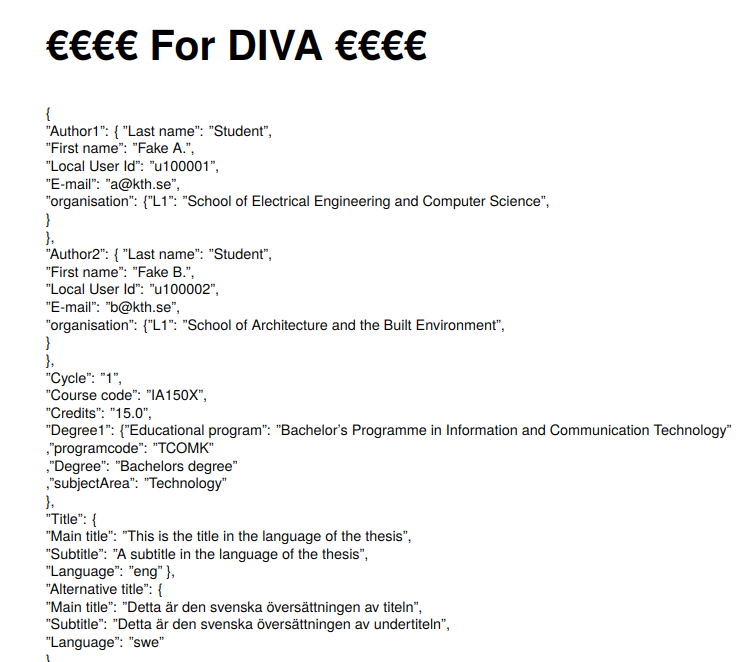
\includegraphics[width=0.99\textwidth]{README_notes/README-examiner-figures/for_diva_top_lines_Screenshot_20220403_164821.png}
  \end{center}
  \caption{Top of the page of data for DiVA}
  \label{fig:topOfForDiva}
\end{figure}
\FloatBarrier

\section{Getting the necessary data}
\label{sec:gettingNecessaryData}
The collected data shown in \Cref{fig:topOfForDiva} is roughly in a format called JavaScript Object Notation (JSON) and described in \Cref{sec:json}. There are several cases to consider for how to extract this information; then, given the information in JSON it is possible to generate a MODS file that can be imported into DiVA:
\begin{itemize}
    \item  \LaTeX~project - as described in \Cref{sec:extractingJSONLaTeX},
    \item DOCX file - as described in \Cref{sec:extractingJSONDOCX}, or
    \item PDF using template - as described in \Cref{sec:extractingJSONPDF}.
\end{itemize}


\subsection {JSON}
\label{sec:json}
JSON is a standard way of representing structured data as text. An example of this text is shown in \Cref{lst:forDIVAtop}. This format is useful as it is \first readily readable by both humans and computers and \Second is easy to edit, and \third is commonly supported by many programming languages. The basic element is of the form: \textquotedbl label\textquotedbl: value\ where label is a string and value can be another string or a structure (an element inside curly braces). String values are within double quote marks. A label of \textquotedbl First name\textquotedbl and the value \textquotedbl Fake A.\textquotedbl~is shown in line \ref{line:firstName} of the listing below. This is part of a structure that gives a value for \textquotedbl Author1\textquotedbl~and this value is a structure with a list of elements for \textquotedbl Last name\textquotedbl, \textquotedbl First name\textquotedbl, \textquotedbl Local User Id\textquotedbl~(\ie the kthid), \textquotedbl E-mail\textquotedbl, and \textquotedbl organisation \textquotedbl. The organisation in turn can have multiple levels where the first level L1 is the school, L2 is a department, and L3 is a division. In a discussion with DiVA administrators at KTH on 2021-04-29, the consensus was that the organizational affiliation of students should be the school of the thesis examiner, since 1\textsuperscript{st} and 2\textsuperscript{nd} cycle students are in \textbf{programs of study} and not schools, department, \etc.

\begin{lstlisting}[language=json, numbers=left,
    stepnumber=1, escapechar=|, caption={Text version of the top of the For DIVA output (reformatted to bring out the structure and improve readability - line numbers are added just in the listing)}, label=lst:forDIVAtop]
{
"Author1": { 
    "Last name": "Student",
    "First name": "Fake A.", |\label{line:firstName}|
    "Local User Id": "u100001",
    "E-mail": "a@kth.se",
    "organisation": {"L1": "School of Electrical Engineering and Computer Science",}
},
"Author2": {
    "Last name": "Student",
    "First name": "Fake B.",
    "Local User Id": "u100002",
    "E-mail": "b@kth.se",
    "organisation": {"L1": "School of Architecture and the Built Environment",}
},
"Cycle": "1",
"Course code": "IA150X",
"Credits": "15.0",
"Degree1": {
    "Educational program": "Bachelor's Programme in Information and Communication Technology",
    "Programcode": "TCOMK",
    "Degree": "Bachelors degree", |\label{line:degree}|
    "subjectArea": "Technology"   |\label{line:subjectarea}|
},
"Title": {
    "Main title": "This is the title in the language of the thesis",
    "Subtitle": "A subtitle in the language of the thesis",
    "Language": "eng" },
"Alternative title": {
    "Main title": "Detta är den svenska översättningen av titeln",
    "Subtitle": "Detta är den svenska översättningen av undertiteln",
    "Language": "swe"
},
\end{lstlisting}

\subsection{Case of \LaTeX~project}
\label{sec:extractingJSONLaTeX}

In the case of an \LaTeX~project, when compiling the \LaTeX~as a side-effect a \texttt{fordiva.json} file is generated, if you save this file locally then you can clean it up and make a MODS file with the following commands:
\Needspace*{4\baselineskip}
\begin{lstlisting}[basicstyle=\footnotesize, language={bash}, caption={Cleanup pseudo JSON produced by the \LaTeX~compiler and then make a MODS file},label=lst:AdmincleanPseudoJSONandConvertToMODS]
./cleanup_pseudo_JSON-from_LaTeX.py --json fordiva.json --acronyms acronyms.tex
./JSON_to_MODS.py --json fordiva-cleaned.json
\end{lstlisting}

Now all you have to do is rename the XML file (\texttt{modsXML.xml}) that was produced to \texttt{xxx.mods} and you are all set to upload the MODS file into DiVA!

To find the \texttt{fordiva.json} file in the \LaTeX project in Overleaf, look for the “Other logs and files” button shown at the bottom of the log output window. After clicking this button you will see a list of log and other files and can now download it.

Note that if the student has used the glossaries package to use acronyms in the abstract(s) they also need to provide an \texttt{acronyms.tex} file.

\generalExpl{Should the student submit the \texttt{fordiva.json} and \texttt{acronyms.tex} file via Canvas (along with their PDF file)?}

\subsection{Case of DOCX file}
\label{sec:extractingJSONDOCX}
In the case of a DOCX file using the template\footnote{The DOCX template (\eg Template-thesis-English-2022-with-for-DiVA.docx is available from available from \url{https://github.com/gqmaguirejr/E-learning} ) while information about using the DOCX template is in the document ``Proposal for a standard thesis template: DOCX version(s)'' available from the same GitHub.}, the JSON data can be extracted directly from the DOCX file and a MODS file created as shown in \Cref{lst:extractDOCX}.
\Needspace*{4\baselineskip}
\begin{lstlisting}[basicstyle=\footnotesize, language={bash}, caption={Extract field values from the DOCX file and then make a MODS file},label=lst:extractDOCX]
./extract_customDocProperties.py filename.docx --json output.json
./JSON_to_MODS.py --json output.json
\end{lstlisting}
If the –-json option is not included in the arguments to\linebreak[4] \texttt{extract\_customDocProperties.py}, the output file is by default “output.json”.

Note that the program can be given an argument of either \texttt{\hbox{–-English}} or \texttt{\hbox{–-Swedish}} to explicitly set the language for the body text. Otherwise, the choice is made based upon the default language (w:lang) specified in the word/settings.xml file.

\warningExpl{Perhaps a custom property for the language of the document should be added.}

The number of pages of the preface and body of the document is taken from the result of the page references to the two bookmarks as generated in the “For DIVA” data. One cannot derive this data directly but only by extracting the data from the word/document.xml file (\textit{after} the word processing package has generated the textual representation for these markers – since their values depends upon the layout and pagination of the document).

A major limitation is that this program only supports extracting English and Swedish abstracts (and keywords); hence abstracts in other languages are \textbf{not} extracted. Additionally, the support for HTML markup in the abstracts is limited to paragraphs. 


\generalExpl{Should the student submit the \texttt{output.json} file via Canvas (along with their PDF file)?}

\subsection{Case of PDF using template file}
\label{sec:extractingJSONPDF}
If all you have is a ``PDF using template file'' then one can extract the information using the program \texttt{extract\_pseudo\_JSON-from\_PDF.py}.  Given a ``PDF using template'' file (and if a \LaTeX~project has been used the acronyms.tex file):
\begin{enumerate}
    \item Save the PDF file of the thesis, for example: \texttt{oscar.pdf}
    \item Extract the “For DIVA” information as JSON, as shown in \Cref{lst:AdminextractPseudoJSONFromPDFforOscarFileToJSON}
    
    If acronyms are used in the abstracts, you can add the “--acronyms acronyms.tex” argument to the extract command line and the program will process the acronyms from the acronyms.tex file (this means that you will also need this file). The output of the program is a JSON file (oscar.json) that can subsequently be used to make an announcement.
\end{enumerate}
\Needspace*{7\baselineskip}
\begin{lstlisting}[basicstyle=\footnotesize, language={bash}, caption={Commands to extract pseudo JSON from the PDF file for Oscar}, label=lst:AdminextractPseudoJSONFromPDFforOscarFileToJSON]    
./extract_pseudo_JSON-from\_PDF.py --pdf oscar.pdf --json oscar.json
./JSON_to_MODS.py --json oscar.json
\end{lstlisting}

\generalExpl{Should the student submit the \texttt{xxxx.json} file and possibly the acronyms.text file via Canvas (along with their PDF file)?}

\subsection{TRITA}
Unless the Office of Student Affairs is going to assign TRITA numbers before the thesis has a cover made, then I think that the Office of Student Affairs has to assign the TRITA number and then \textbf{make and apply the cover}. The current method of making and applying covers before the PDF is submitted to the Office of Student Affairs is foolish and unnecessary. It is easy to specify the TRITA string as an argument when making the MODS file, as shown in \Cref{lst:specifyTRITA}. 
\begin{lstlisting}[basicstyle=\footnotesize, language={bash}, caption={Command to make a MODS file with a specified TRITA string}, label=lst:specifyTRITA]
./JSON_to_MODS.py --json fordiva.json --trita "TRITA-XXX-EX-2021:219"
\end{lstlisting}

This requires that the student provide the information about the degree that they will apply for and the subject area \textbf{within} their document so that it ends up in the JSON file. This was done in lines  \ref{line:degree} and \ref{line:subjectarea} in \Cref{lst:forDIVAtop}.

\subsection{Covers}
A DOCX cover can be made for a thesis using the \texttt{JSON\_to\_DOCX\_cover.py} command shown in \Cref{lst:JSONtoDOCXcover}. This command supports the many different types of exams. It also can take many optional parameters that will over ride the contents of the JSON file (by default the JSON file name is assumed to be \texttt{calendar\_event.json}) as shown in \Cref{lst:JSONtoDOCXcover2}. If the \texttt{\hbox{-\,-language sv}} command is used or the language of the main title is Swedish (indicate in the JSON file as `swe'') the program eliminates the English KTH logotype and changes the course name appropriately. The field of technology or main subject have to be in the selected language, shown in \Cref{lst:JSONtoDOCXcover2}. Note that you can optionally specify the TRITA string on the command line with an option of the form:
\texttt{\hbox{-\,-TRITA  "TRITA-XXX-EX-2022:99999"}}.

\begin{lstlisting}[escapechar=|, basicstyle=\footnotesize, language={bash}, caption={Command to make a cover DOCX file with a specified TRITA string}, label=lst:JSONtoDOCXcover]
./JSON_to_DOCX_cover.py --file  Omslag_Exjobb_Eng_en-20220325.docx |\textbackslash \\| --exam kandidatexamen  --trita "TRITA-XXX-EX-2021:0000"
\end{lstlisting}

\begin{lstlisting}[escapechar=|, basicstyle=\footnotesize, language={bash}, caption={Command to make a cover DOCX file with the specified values}, label=lst:JSONtoDOCXcover2]
./JSON_to_DOCX_cover.py --file Omslag_Exjobb_Eng_en-20220325.docx|\textbackslash \\| --cycle 2 --credits 30.0 --area "bioteknik" --area2 "kemiteknik"|\textbackslash \\| --exam both --trita "TRITA-CBH-EX-2021:00"|\textbackslash \\| --language sv  --json calendar-sv.json
\end{lstlisting}

\textbf{NB}: The program is explicitly designed to work with the English version of the template from 2022-03-25, hence the specification of the template used in the two examples above.

\warningExpl{TODO: Make a program to make and apply the correct cover to the PDF file. Otherwise, one can use the specific templates shown at \url{https://canvas.kth.se/courses/11/pages/templates-for-1st-and-2nd-cycle-theses-some-templates}.}

\textbf{NB}: The current \LaTeX~template makes the front and back covers and uses a TRITA string specified in the \LaTeX~project files. The command shown in \Cref{lst:specifyTRITA} overrides this value when making the MODS file, but the existing TRITA string on the back cover has to be manually edited.

\warningExpl{Perhaps a solution is to integrate the \textbf{front} cover into both the \LaTeX and the DOCX templates and have the Office of Student Affairs apply only the back cover - as this is where the TRITA number appears.}

\textbf{NB}: The ``For DIVA'' pages need to be removed from the PDF file before uploading the PDF file into DiVA.

\section[Inserting information into LADOK]{Inserting information into LADOK}
\label{sec:JSONtoLADOKDiVAAdmis}
As part of the effort to be able to minimize the effort of cutting and pasting. I have made a program JSON\_to\_ladok.py that takes the extracted JSON information and uses the information about the author(s) and the title and alternative title to try to insert this information into LADOK for the module (\ie ``moment'' in Swedish) that requires a project title, \ie, 'KravPaProjekttitel' is True. \Cref{lst:usingExtractedJSONtoProduceLADOKentry1} shows an example of using this program to try to put the title and alternative title into LADOK. Basically the program logic should work, but I do \textbf{not} have the required permission to make entries of this sort of data for a degree project (\ie Rapporteringsrättighet saknas).

Note that this program uses the \texttt{ladok3} python library but extends it with some features that are not (yet) in the library. \textbf{It should be regarded as very much a work in progress.} However, it illustrates what could be done using the information in the JSON file.
\begin{lstlisting}[language={bash},
    breaklines=true,
    breakatwhitespace=true,          % sets if automatic breaks should only happen at whitespace
    breakindent=0em,
    caption={Using the extracted JSON to produce a LADOK entry for a student in the DA231X degree project course}, label=lst:usingExtractedJSONtoProduceLADOKentry1]
./JSON_to_ladok.py --json xxx.json 
...
author={'Last name': 'xxx', 'First name': 'yyy', 'Local User Id': 'u1xxxx', 'E-mail': 'oxxx@kth.se', 'organisation': {'L1': 'School of Electrical Engineering and Computer Science '}}
Canvas user_id=dddd
integration_id=gggggg-gggg-gggg-gggg-ggggggg
ladoK_course_info={'id': '6683207e-5a5d-11eb-9b32-eeb44fb14647', 'round_id': '8e15ae14-1d86-11ea-a622-3565135944de', 'education_id': '374ea085-73d8-11e8-afa7-8e408e694e54', 'instance_id': '8eee8da9-dd0a-11e8-bb7a-19f8cd1a470e', 'swe_name': 'Examensarbete i datalogi och datateknik, avancerad nivå', 'eng_name': 'Degree Project in Computer Science and Engineering, Second Cycle'}
moment code=PRO1, requires title=False
moment code=PRO2, requires title=False
moment code=PRO3, requires title=True
trying to store a passing grade for moment=PRO3
Traceback (most recent call last):
  File "./JSON_to_ladok.py", line 533, in <module>
    sys.exit(main(sys.argv[1:]))
  File "./JSON_to_ ladok.py", line 519, in main
    status=save_result_degree_project3(ladok, integration_id, course_code, mom['Utbildningskod'], '2021-07-14', 'P', "PF", main_title, alternative_main_title)
  File "./JSON_to_ ladok.py", line 374, in save_result_degree_project3
    raise Exception("Couldn't register " + course_moment + "=" + grade_raw + " " + result_date_raw + ": " + r.json()["Meddelande"])
Exception: Couldn't register PRO3=P 2021-07-14: Hinder mot skapa resultat påträffat: Rapporteringsrättighet saknas
\end{lstlisting}

\warningExpl{There is currently a transfer to LADOK project within the group of developers at the IT unit who are working on E-learning - they have been working on an API for entering the title(s) and other information (just as they are making it possible to use a program to enter grades and dates for other courses).}


\section{The examiners can also use the JSON file}

\Cref{fig:overallDataflow} shows the overall data flow starting with either a DOCX document or \LaTeX\~project that has used the thesis templates. Not only is the JSON data useful with respect to DiVA, but it can also be used for other purposes. For example, as shown in \Cref{fig:overallDataflow}, an examiner can use it for announcing the student's oral presentation via the Canvas course room and calendar and potentially in the KTH Cortina Calendar.

However, as calendar entries were not relevant to DiVA administrators, this figure was simplified in \Cref{fig:forDiVAAdmins}.

\begin{figure}[!ht]
\resizebox{1\textwidth}{!}{%
\begin{tikzpicture}
[align=left,node distance=2cm]



\node (DOCXFile) [tape,tape bend top=none,draw,font=\sffamily] {DOCX using template};
\node (latexFile) [tape,tape bend top=none,draw,font=\sffamily, right=0.5cm of DOCXFile] {\LaTeX project using template};




\node (LaTeX) [processBox,  below=5cm of latexFile] {LaTeX compiler};
%\node (acronymsfile) [tape,tape bend top=none,draw,font=\sffamily, right=2cm of latexFile] {acronyms.tex};
\node (latexjsonFile) [tape,tape bend top=none,draw,font=\sffamily, below of=LaTeX] {fordiva.json};



\node (extractDOCX) [processBox, below=8cm of DOCXFile] {extract\_custom\_DOCX\_properties};
\node (PDFfile) [tape,tape bend top=none,draw,font=\sffamily, left=5cm of LaTeX] {PDF using template};
\node (Word) [processBox,  above=3cm of PDFfile] {Word or similar};
\node (extractor) [processBox, below=6cm of PDFfile] {extract\_pseudo\_JSON-from\_PDF};

\node (cleanJSONfromLaTeX) [processBox, below=4cm of LaTeX] {cleanup\_pseudo\_JSON-from\_LaTeX};
\node (jsonFile) [tape,tape bend top=none,draw,font=\sffamily, below=4cm of cleanJSONfromLaTeX] {JSON file};

\node (start) [processBox, right=0.5cm of jsonFile] {JSON\_to\_calendar};

\node (assignTRITA) [processBox, below=3cm of jsonFile] {Assign TRITA number};
\node (jsonFileWithTRITA) [tape,tape bend top=none,draw,font=\sffamily, below of=assignTRITA] {JSON file with TRITA};
\node (jsontoMODS) [processBox, below of=jsonFileWithTRITA] {JSON\_to\_MODS};
%\node (modsFile) [tape,tape bend top=none,draw,font=\sffamily, below of=jsontoMODS] {MODS file};

\node (calendarEvent) [destinationBox, right=1cm of start] {Canvas calendar event};
\node (announcement) [destinationBox,  above of =calendarEvent] {Canvas announcement};
\node (acronymsfile) [tape,tape bend top=none,draw,font=\sffamily, right=4.5cm of cleanJSONfromLaTeX] {acronyms.tex};
\node (cortinaCalendarEvent) [destinationBox,  right=0.5cm of start, below of=calendarEvent] {KTH Cortina calendar event};
\node (TRITAlist) [destinationBox, right=1cm of assignTRITA] {TRITA list/database};

\node (modsFileWithTRITA) [tape,tape bend top=none,draw,font=\sffamily, below of=jsontoMODS] {MODS file with TRITA};
\node (makeApplyCover) [processBox, below of=modsFileWithTRITA] {Make and apply cover};
\node (divameta) [destinationBox, right=1cm of modsFileWithTRITA] {Import MODS file into DiVA};
\node (diva) [destinationBox, right=1cm of makeApplyCover] {Upload PDF into DiVA};


\draw [red, dashed]   (PDFfile) to[out=-120,in=180] (makeApplyCover);
\draw [red, dashed]   (Word) to[out=-90,in=90] (PDFfile);
\draw [red, dashed]   (LaTeX) to[out=-180,in=90] (PDFfile);
\draw [arrow] (DOCXFile) --  (extractDOCX.north);
\draw [arrow] (extractDOCX) --  (jsonFile.north west);
\draw [arrow] (latexFile.south) --  (LaTeX.north);
\draw [arrow] (LaTeX) --  (latexjsonFile.north);
\draw [arrow] (latexjsonFile) --  (cleanJSONfromLaTeX.north);
\draw [arrow] (cleanJSONfromLaTeX.south) --  (jsonFile.north);
\draw [red, dashed] (PDFfile) --  (extractor.north);
\draw [arrow] (DOCXFile) --  (Word.north);
\draw [arrow] (extractor.south) --  (jsonFile.west);
\draw [arrow] (jsonFile) --  (assignTRITA);
\draw [arrow] (jsonFile) --  (start.west);
\draw [arrow] (start.east) --  (announcement.west);
\draw [arrow] (start.east) -- (calendarEvent);
\draw [arrow] (start.east) -- (cortinaCalendarEvent.west);
%\draw [arrow] (jsonFile) --  (jsontoMODS.north west);
%\draw [arrow] (jsontoMODS) --  (modsFile);
%\draw [arrow] (jsontoMODS) --  (modsFile);
\draw [arrow] (jsontoMODS) --  (modsFileWithTRITA);
%\draw [arrow] (modsFile) --  (assignTRITA);
\draw [arrow] (modsFileWithTRITA) --  (divameta);
\draw [arrow] (assignTRITA) --  (jsonFileWithTRITA);
\draw [arrow] (jsonFileWithTRITA) --  (jsontoMODS);
\draw [arrow] (modsFileWithTRITA) --  (makeApplyCover);
\draw [arrow] (makeApplyCover) --  (diva);
%\draw [arrow] (assignTRITA) --  (modsFileWithTRITA);
\draw [arrow] (latexFile.south east) --  (acronymsfile.north);
\draw [arrow] (acronymsfile.south east) to[out=-45,in=0]  (jsontoMODS.east);
\draw [arrow] (TRITAlist) --  (assignTRITA.east);
\draw [arrow] (assignTRITA) --  (TRITAlist.west);

\end{tikzpicture}
}
\caption[Overall data flow]{Overall data flow from a DOCX document and a \LaTeX\~project using the templates. The figure shows the flow of data - the dashed red line shows the PDF, while the black lines show other types of data}
  \label{fig:overallDataflow}
\end{figure}
\FloatBarrier
\section{Open questions}
Some of the open questions are:
\begin{itemize}
    \item What should the student submit (via the examiner or via Canvas?)?
    \item What should the Office of Student Affairs do?
\end{itemize}

\section{Final notes}
\textbf{Best of success in using the programs!} If there are questions, contact me at  \href{mailto:maguire@kth.se}{maguire@kth.se}
.

%\end{document}

\fi
\end{comment}

\begin{comment}
% Information for Course Coordinators
\ifxeorlua
\cleardoublepage

\chapter{README and notes for course responsible persons}
\label{ch:readme_course_responible}

Given that students are going to be in Canvas course rooms and that they are likely to use a version of a template, how can the Canvas course room be set up to make it efficient for students, teachers, administrators, \etc?

\section{Custom columns}
\label{sec:CRcustomeCOlumns}

One of the first steps is to create some custom columns to be used to store information that is only visible to teachers in the course. What are some useful columns:
\begin{description}[labelwidth =\widthof{\textbf{Tentative\_title}}, leftmargin = !]
\item[Tentative\_title]  The working title - initially taken from the proposal

\item[TRITA] To store the TRITA numbers of theses that have been reported in LADOK

\item[Supervisors] Store the supervisors as a comma-separated list of names-

\item[Group] In a degree project course for 1\textsuperscript{st} students, it is useful to be able to store the name of the group, so that one can sort the gradebook based on this field and thus have the group members adjacent in the gradebook.
\end{description}

Custom columns can be added using a Python script, such as the three calls to the script shown in \Cref{lst:CRaddingCustomCOlumns}.
\Needspace*{4\baselineskip}
\begin{lstlisting}[basicstyle=\footnotesize, language={bash}, columns=fullflexible, showstringspaces=false, caption={Adding custom columns to the gradebook},label=lst:CRaddingCustomCOlumns]
insert-column.py 40135 'TRITA'
insert-column.py 40135 'Tentative_title'
insert-column.py 40135 'Supervisors'
\end{lstlisting}

As the list of supervisors can vary over time, a custom column called ``Supervisors'' has been generated that contains a list of the names of the supervisors; for example: ['Anders Västberg', 'Gerald Maguire']. Note that because this list uses a version of the person's name\footnote{In the case of some individuals, there are multiple versions of their name that have been used, so the mapping supports a many-to-one mapping - as there is only one version of the user's name in Canvas.} that may not be the same as the user's Canvas name, a file containing a mapping between these names and the corresponding user's name in Canvas is needed by scripts. As with all custom columns, this column is only visible to teachers in the course.


\section{Administrative assignments}
\label{sec:CRAdministrativeAssignments}

In this case, an ``administrative'' assignment is used that has as its grade scheme a list of all of the examiners in the course. Thus in the grade book, the ``Examiner'' assignment has a ``grade'' for each student that indicates who the examiner is for that student.  This grading scheme can be automatically generated from the set of people who have the Examiner role in this Canvas course room (this is done using the command shown in \Cref{lst:CRaddingGradingStandardA}). Additionally, there is a section in the course created for each examiner (using the sortable version of the examiner's name from Canvas) so that when the student is added to the examiner's section - the examiner can filter their view in the gradebook to see just the students in their section - this makes it much easier for working with the subset of students relevant to this person. This ``administrative'' assignment is not published - so it is only visible to teachers in the course.

Grading standards, \ie a grading scale) can be added using a Python script, such as that shown in \Cref{lst:CRaddingGradingStandardA,lst:CRaddingGradingStandardB}.
\begin{lstlisting}[basicstyle=\footnotesize, language={bash}, columns=fullflexible, showstringspaces=false, caption={Adding a grading standard for all of the examiners to the course},label=lst:CRaddingGradingStandardA]
./insert_teachers_grading_standard.py -e 40135 --examiners
\end{lstlisting}

Another ``administrative'' assignment called ``Course code'' is used similarly to the Examiner ``administrative'' assignment but now uses all of the courses codes used in this course room as the grading scheme. This column is populated based on the short version of the course code, such as ``DA231X'' taken from the name of the section names with the course codes that the student is in within this course room. The command for doing this is shown in \Cref{lst:CRaddingGradingStandardA}).
\begin{lstlisting}[basicstyle=\footnotesize, language={bash}, columns=fullflexible, showstringspaces=false, caption={Adding grade standard for the course codes to the course},label=lst:CRaddingGradingStandardB]
./insert_course_code_grading_standard.py 40135
\end{lstlisting}

\section{Utilizing sections in the Canvas course room}
\label{sec:CRUsingSectionc}


Sections are also generated for each of the teachers in the course so that students can be added to their section, and the teacher can filter the gradebook to see just the relevant students. 
 The command for doing this is shown in \Cref{lst:CRcreatSectionsForTeachers}). The sortable name for each teacher (\ie last\_name, first\_name) is used for the name of the section.
\begin{lstlisting}[basicstyle=\footnotesize, language={bash}, columns=fullflexible, showstringspaces=false, caption={Create a section for each teacher in the course},label=lst:CRcreatSectionsForTeachers]
./create_sections_for_teachers-in-course.py 40135
\end{lstlisting}

\fi
\end{comment}

%% The following label is necessary for computing the last page number of the body of the report to include in the "For DIVA" information
\label{pg:lastPageofMainmatter}

\cleardoublepage
\clearpage\thispagestyle{empty}\mbox{} % empty page with backcover on the other side
\kthbackcover
\fancyhead{}  % Do not use header on this extra page or pages
\section*{€€€€ For DIVA €€€€}
\lstset{numbers=none} %% remove any list line numbering
\divainfo{pg:lastPageofPreface}{pg:lastPageofMainmatter}

% If there is an acronyms.tex file,
% add it to the end of the For DIVA information
% so that it can be used with the abstracts
% Note that the option "nolol" stops it from being listed in the List of Listings

% The following bit of ugliness is because of the problems PDFLaTeX has handling a non-breaking hyphen
% unless it is converted to UTF-8 encoding.
% If you do not use such characters in your acronyms, this could be simplified.
\ifxeorlua
\IfFileExists{lib/acronyms.tex}{
\section*{acronyms.tex}
\lstinputlisting[language={[LaTeX]TeX}, nolol, basicstyle=\ttfamily\color{black},
commentstyle=\color{black}, backgroundcolor=\color{white}]{lib/acronyms.tex}
}
{}
\else
\IfFileExists{lib/acronyms-for-pdflatex.tex}{
\section*{acronyms.tex}
\lstinputlisting[language={[LaTeX]TeX}, nolol, basicstyle=\ttfamily\color{black},
commentstyle=\color{black}, backgroundcolor=\color{white}]{lib/acronyms-for-pdflatex.tex}
}
{}
\fi


\end{document}
